\documentclass[a4paper]{book}
\usepackage{makeidx}
\usepackage{graphicx}
\usepackage{multicol}
\usepackage{float}
\usepackage{listings}
\usepackage{color}
\usepackage{ifthen}
\usepackage[table]{xcolor}
\usepackage{textcomp}
\usepackage{alltt}
\usepackage{ifpdf}
\ifpdf
\usepackage[pdftex,
            pagebackref=true,
            colorlinks=true,
            linkcolor=blue,
            unicode
           ]{hyperref}
\else
\usepackage[ps2pdf,
            pagebackref=true,
            colorlinks=true,
            linkcolor=blue,
            unicode
           ]{hyperref}
\usepackage{pspicture}
\fi
\usepackage[utf8]{inputenc}
\usepackage{mathptmx}
\usepackage[scaled=.90]{helvet}
\usepackage{courier}
\usepackage{doxygen}
\lstset{language=C++,inputencoding=utf8,basicstyle=\footnotesize,breaklines=true,breakatwhitespace=true,tabsize=8,numbers=left }
\makeindex
\setcounter{tocdepth}{3}
\renewcommand{\footrulewidth}{0.4pt}
\begin{document}
\hypersetup{pageanchor=false}
\begin{titlepage}
\vspace*{7cm}
\begin{center}
{\Large DivWin \\[1ex]\large 1.0v }\\
\vspace*{1cm}
{\large Generated by Doxygen 1.7.3}\\
\vspace*{0.5cm}
{\small Sun Sep 11 2011 13:58:39}\\
\end{center}
\end{titlepage}
\clearemptydoublepage
\pagenumbering{roman}
\tableofcontents
\clearemptydoublepage
\pagenumbering{arabic}
\hypersetup{pageanchor=true}
\chapter{1.Using DivWin}
\label{DivWinExplanation}
\hypertarget{DivWinExplanation}{}
\hyperlink{_w_t_div_win_8h_source}{WTDivWin.h}

Using DivWin by William Thorley

DivWin is based on a Process / Renderable Object mentality. Process' are classes with behavioural code which tell them how to behave. They take inputs from the OS, signal other process' and tell Renderable objects how to display. Once a Process is written, the user should create a new instance. The system will record the information add it to the system and make the process enact it's behaviour, with no further input form the user (Fire and Forget). This way many similar objects can be created easily once the behavioural code is written. Render Objects should not have any behavioural code and are entirely directed by Process'.

The Process' are controlled by \hyperlink{classc_kernel}{cKernel} which will track and update all the process'.

Render Objects actually display on the screen. They are moved around in 3D space and \hyperlink{classc_camera}{cCamera} renders them to the screen.

Collision Objects must be handed a Render Object at startup, which they will follow and determine collisions with other Collision Objects.

Files are loaded by the FileHandler and can be asked to provide media data for Render Objects and Collision Objects.

Lighting effects are controlled by the LightHandler.

The Main Loop:


\begin{DoxyCode}
*#include <WTDivWin.h>
*int WINAPI WinMain (HINSTANCE hInstance,
                    HINSTANCE hPrevInstance,
                    LPSTR lpCmdLine,
                    int iCmdShow)
*{
 //_START_PROGRAM(First_Process_Type,User_Settings_Type,Instance);  
 return _START_PROGRAM(cCore,cUserSettings,hInstance);

};
*
\end{DoxyCode}
 
\begin{DoxyCode}
 //Using DivWin in Linux
*#include <WTDivWin.h>

*int main ()
*{
  //_START_PROGRAM(First_Process_Type,User_Settings_Type); 
  return _START_PROGRAM(cCore,cUserSettings);

*}
*
\end{DoxyCode}


Main Loop Explanation: This will call the main function which will initialise the various components of the system. First\_\-Process\_\-Type must be a class type which inherits \hyperlink{classc_process}{cProcess} and should be the process that initialises and creates all the other processes required for the game. User\_\-Settings\_\-Type must be a class type which inherits \hyperlink{classc_settings}{cSettings}. The virtual function UserSettings() in the derived class should set all the variables the user wishes to define. If the User does not wish to define ANY settings, use \hyperlink{classc_settings}{cSettings} here and the defaults will be used. hInstance is a Windows only variable which is passed from the operating system to the WinMain function. Use the first HINSTANCE Passed to the function.\par
 First \_\-START\_\-PROGRAM will set the settings for the game to use.\par
 Then it will initialise the various components of the engine.\par
 It will create an instance of the class type First\_\-Process\_\-Type which should initilise the game and create other processes to start the game.\par
 While there are processes alive (and the system has not received an exit signal) the system will continue to cycle.\par
 As the system exit, it will clear data, close links to devices and hardware and return a suitable exit signal for the Operating system. This should be returned from the funciton main().\par
 
\chapter{2. Using the cKernel}
\label{cKernelExplanation}
\hypertarget{cKernelExplanation}{}
\hyperlink{_w_t_kernel_8h_source}{WTKernel.h}

Using the kernel system by William Thorley

The kernel will create itself as soon as any Process is created. It will automatically link the process, and sort their run order. A Pointer to the \hyperlink{classc_kernel}{cKernel} can always be found by calling the macro \_\-KERNEL (\hyperlink{classc_kernel_a5bd65ef494632b9fd585a6f6cae375e7}{cKernel::Instance()}). If this function is called and there is no \hyperlink{classc_kernel}{cKernel}, the function will create one. The Constructor is private, so there can be only one \hyperlink{classc_kernel}{cKernel}. The Kernel is entirely automatic and should require no inputs from the user. However it can supply useful information and functionality to the user. KillAll(): Calling KillAll() will kill every running process. This will cause Update() to exit, and traditionally end the program. However it is possible to KillAll(), then create a new core process, and call Update() again, thereby ‘restarting’ the program.

\_\-FIND\_\-PROCESS(TYPE) Calling \_\-FIND\_\-PROCESS() will automatically search the \hyperlink{classc_kernel}{cKernel} for any processes of class type TYPE. It will return a pointer to the next process of class type TYPE everytime it is called. When there are no more processes of class type TYPE it will return 0. 
\chapter{3. The First Process}
\label{CoreExamples}
\hypertarget{CoreExamples}{}
\hyperlink{_w_tc_process_8h_source}{WTcProcess.h}

Using William Thorley’s Process system

The First Process is exactly the same as every other process. i.e. it must inherit \hyperlink{classc_process}{cProcess}. What is special about the Process passed to the \_\-START\_\-PROGRAM() call is that it is the automatically called when the Kernel is initialized. This means that the loading code for cCore is the initialization code for the entire program. Usually the process’ which will form the program are started here as well as loading files for the system. For these examples I wil call the class cCore.

This shows the declaration for cCore. Using \_\-PROCESS(Type) is the same as calling class Type : public \hyperlink{classc_process}{cProcess} to inherit \hyperlink{classc_process}{cProcess}. Declaration: 
\begin{DoxyCode}
 _PROCESS(cCore)
 {
  public:
  cCore();
 
  void Run();
 
  ~cCore();
 
 void AdditionalKillFunctionality();
 void AdditionalSleepFunctionality();
 void AdditionalWakeFunctionality();
 
 };
\end{DoxyCode}


cCore(): This shows the constructor for cCore. As it is the first object it will load media for the rest of the program and kick off the other processes. 
\begin{DoxyCode}
 cCore::cCore()
 {
 //Load IMF Files into memory.
  _LOAD_FILE("../src/User/Models/AShipModel.imf");
  _LOAD_FILE("../src/User/Models/StartShip.imf");
  _LOAD_FILE("../src/User/Textures/ATexture.imf");
  _LOAD_FILE("../src/User/CollisionObjects/ACollision.imf");
  _LOAD_FILE("../src/User/Objects/AIMFFileWithSeveralComponents.imf");

 // Setup the camera.
  _CAMERA->Far(1000.0f);
  _CAMERA->Frustum();
 
 //Create a new process and a renderable object.
  mpProcessPointer=_CREATE(MyFirstProcess());
  mpRenderObjectPointer=_CREATE(MyFirstRenderObject());

 }
\end{DoxyCode}


Run(): Run() is run once every frame as long as cCore is alive and controls the entire program. The Run() function should is explicity designed to be re-\/written by the user to give each \hyperlink{classc_process}{cProcess} class their functionality. This Code can be seen as the behaviour that the process should follow. It should rotate and position the Process' Renderobjects, send signals, receive inputs, anything the Process may want to do as part of it's behaviour. The function cCore::Run() can be used like any other process, but is usually used to oversee the running of the program. 
\begin{DoxyCode}
 void cCore::Run()
 {

  if(_KEY(KEY_SPACE)) _CAMERA->Far(10.0f);
   else _CAMERA->Far(1000.0f);
  _CAMERA->Frustum();

  mpProcessPointer=_CREATE(MyFirstProcess());
  mpRenderObjectPointer=_CREATE(MYFirstRenderObject());

 }
\end{DoxyCode}


$\sim$cCore(): This is called when the object is deleted, not when it is killed. It is difficult to predict reliably where this will be called, so it is best not to put code in this function.

AdditionalKillFunctionality(): This is called whenever the cCore Process is Killed. This will only activate if the process was alive and is now dead. This should be used to kill or transfer control of Render Objects that are owned by this process, or unload files that are no longer used.


\begin{DoxyCode}
 *void cCore::AdditionalKillFunctionality()
 *{
 _KILL(mpRenderObjectPointer);
 mpProcessPointer_SIGNAL(_S_SLEEP);
         *}
         *
\end{DoxyCode}


AdditionalSleepFunctionality(): This is called whenever the cCore Process is made to Sleep. This will only activate if the process was awake and is now asleep. This is generally used to sleep Render Objects that are owned by this process.


\begin{DoxyCode}
         *void cCore::AdditionalSleepFunctionality()
         *{
 mpRenderObjectPointer->Signal(_S_SLEEP);
                 *}
                 *
\end{DoxyCode}


AdditionalWakeFunctionality(): This is called whenever the cCore Process is made to Wake. This will only activate if the process was asleep and is now awake. This is generally used to wake Render Objects that were slept when cCore was sent to sleep.

void cCore::AdditionalSleepFunctionality() \{ mpRenderObjectPointer-\/$>$Signal(\_\-S\_\-WAKE); \}  
\chapter{4. How to use Process Objects}
\label{ProcessExplanation}
\hypertarget{ProcessExplanation}{}
\hyperlink{_w_tc_process_8h_source}{WTcProcess.h}

Using William Thorley’s Process Handler System

When properly implemented the process handler automatically links and runs all processes. A process must inherit \hyperlink{classc_process}{cProcess}. It must also define the virtual function Run() a process without a Run() function is useless, and will be deleted during the frame it is created.

Declaring a new process class called player: 
\begin{DoxyCode}
 //This is the same as _PROCESS(player)
 *class player : public cProcess
 *{
         *public :
         void Run();
         *};
         *
\end{DoxyCode}


void \hyperlink{classc_process_a3e0fab4ccc0a8fb065d50eb88b6a0dd5}{cProcess::Run()}; The function Run() is a virtual function already defined. This function is called every time the process must run its code (usually once a frame). The code that defines how the process acts goes in Run().

Creating a Process: Call the macro \_\-CREATE(Type); This will return a pointer to the new process of type Type. 
\begin{DoxyCode}
 player *mpNewProcessPointer;
 NewProcessPointer=_CREATE(player());
 _CREATE(AnotherProcess(Argument1,Argument2));
\end{DoxyCode}


Killing a Process: Process' must not be destroyed by deleting the process. Processes can be be deleted either by calling the macro \_\-KILL(); or by calling the Function Signal(SIGNAL lsFlags) with the flag \_\-S\_\-KILL. if \_\-KILL() is called without a pointer it will automatically use the pointer this. Process' will not be destroyed when the signal is sent, they will be deacticated, but the memory will remain allocated until \hyperlink{classc_kernel}{cKernel} reaches the correct stage to delete the object. Objects can remain allocated into the next frame, but not the frame after that. Both pieces of following code have the same effect. The Process pointed to by mpPointerToAnotherProcess is Killed and then this process is killed. 
\begin{DoxyCode}
 void player::Run()
 {

 if(_KEY(KEY_k))
 {
 mpPointerToAnotherProcess->Signal(_S_KILL);
 _KILL(this);
 }

 }
\end{DoxyCode}



\begin{DoxyCode}
 void player::Run()
 {

 if(_KEY(KEY_k))
 {
 _KILL(mpPointerToAnotherProcess);
 _KILL();
 }

 }
\end{DoxyCode}


Sleeping a Process: A Process can be sent to sleep by calling the \hyperlink{classc_signal_a77af8271fc7ffb8696ba73a01e213808}{cSignal::Signal(SIGNAL lsFlags)} function with the value \_\-S\_\-SLEEP. Sleeping a process leaves the process in the process list, but stops the Run() function being called every frame. This allows the Signal(SIGNAL lsFlags) function to be used to return it to ‘active duty’. The memory will remain allocated. Sending repeated Sleep calls to a process will not affect the process or the stability of the system, the Process will remain asleep.

Waking a Process: A Process can be awakend by calling the \hyperlink{classc_signal_a77af8271fc7ffb8696ba73a01e213808}{cSignal::Signal(SIGNAL lsFlags)} function with the value \_\-S\_\-WAKE. Sending repeated Waking calls to a process will not affect the process or the stability of the system, the Process will remain awake. 
\begin{DoxyCode}
 void player::Run()
 {

 if(_KEY(KEY_s)) mpPointerToAnotherProcess->Signal(_S_SLEEP);
 if(_KEY(KEY_w)) mpPointerToAnotherProcess->Signal(_S_WAKE);

 }
\end{DoxyCode}


Removing a Process: A Process can be killed by the \hyperlink{classc_kernel}{cKernel} object. Calling the \hyperlink{classc_kernel_a59c9a956e6a6666a57c2d85e463381d8}{cKernel::Remove()} function will kill the process and free the memory. This must not be done to the currently running process or the system may crash. Use on the current process at your peril. The pointer is to the \hyperlink{classc_linked_node}{cLinkedNode$<$vProcess$>$} which owns this process. Each Process has a pointer (mpNode) to its \hyperlink{classc_linked_node}{cLinkedNode$<$vProcess$>$}. $\ast$ 
\begin{DoxyCode}
 void player::Run()
 {

 if(_KEY(KEY_k)) _KERNEL->Remove(mpPointerToAProcessesNode);

 }
\end{DoxyCode}
 
\chapter{5. How to use Render Objects}
\label{RenderObjectExplanation}
\hypertarget{RenderObjectExplanation}{}
\hyperlink{_w_tc_render_object_8h_source}{WTcRenderObject.h}

Using William Thorley’s Renderable Object System

All Render Objects are inherited from class \hyperlink{classv_render_object}{vRenderObject}, through class \hyperlink{classc_render_object}{cRenderObject}. The object also Inherits the class \hyperlink{classc_matrix4}{cMatrix4}. This is a 3D Translation class, and can handle 2D rotations (about X axis), 3D rotations, 3D Translations and 3D scaling. Calling the \hyperlink{classc_matrix4}{cMatrix4} functions will move the \hyperlink{classc_render_object}{cRenderObject}.

Creating RenderObjects: cRenderObjects can be created using the \_\-CREATE macro as per a Process. This will return a pointer to the RenderObject. 
\begin{DoxyCode}
 void player::Run()
 {
        mpHull=_CREATE(cTexturedModel(mpShipNode));
        mpHull->Mesh(_GET_FILE(vMesh*,"Mesh"));
        mpHull->Texture(_GET_FILE(vTexture*,"Texture"));
        mpHull->Shader(_GET_SHADER("TexturingProgram"));
 }
 *
\end{DoxyCode}


Currently there are lots of Render Objects:

class \hyperlink{classc_textured_model}{cTexturedModel}; class \hyperlink{classc_landscape}{cLandscape}; class \hyperlink{classc_render_node}{cRenderNode}; class \hyperlink{classc_beam_mesh}{cBeamMesh}; class \hyperlink{classc_image}{cImage}; class cTextureText; class \hyperlink{classc_line}{cLine}; class \hyperlink{classc_particle}{cParticle}; class \hyperlink{classc_particle_group}{cParticleGroup}; class \hyperlink{classc_particle_handler}{cParticleHandler}; class \hyperlink{classc_model_list}{cModelList}; class \hyperlink{classc_point}{cPoint};

See the relevant documentation for each for how to use them.

The Renderable Object allows the user to develop their own Renderable Objects and links them to the renderer. A Renderable object must inherit \hyperlink{classc_render_object}{cRenderObject} and must also define the virtual function Render(), This will be called every time the renderable object needs to be rendered. It should also define all empty virtual functions in \hyperlink{classv_render_object}{vRenderObject} and \hyperlink{classc_render_object}{cRenderObject},

Declaration of a Renderable Object: class player : public \hyperlink{classc_render_object}{cRenderObject}, public \hyperlink{classc_matrix4}{cMatrix4} \{ public : Render(); \};

Render(): 
\chapter{6. Use of the cMatrix4 and cCameraMatrix Classes}
\label{Matrix4Explanation}
\hypertarget{Matrix4Explanation}{}
\par
 cMatrix4.h \par
 cCameraMatrix.h \par
 \par
 Use of the Translation matrix classes by William Thorley. \par
 \par
 The \hyperlink{classc_matrix4}{cMatrix4} class and cCameraMatrix classes are very similar. The CameraMatrix maintains an inverted \hyperlink{classc_matrix4}{cMatrix4} matrix as the translations applied to the camera must be inverted to give the same effect as to normal objects. Otherwise the effects are the same for \hyperlink{classc_matrix4}{cMatrix4} and cCameraMatrix. \par
 Most Render Objects have inherited the \hyperlink{classc_matrix4}{cMatrix4} class meaning that these functions can be called to move and rotate Render Objects. Calling these functions, will apply the defined translations to the current object. Some are relative to the current translation and some are relative to the position of the Render Node controlling this object. Either way, the translations stack. \par
 \par
 The X Axis points 90 to the Right perpendicular to the objects facing. \par
 The Y Axis points 90 Upwards, perpendicular to the objects facing. \par
 The Z Axis is the objects facing. \par
 \par
 These Classes can be used for 2D or 3D Translations. There are different functions for 2D and 3D translations. The standard DivWin Objects automatically identify if they should be 2D or 3D. \par
 \par
 3D Object Translation Functions: \par
 void Set3D() \par
 \par
 float $\ast$Position() \par
 float X() \par
 float Y() \par
 float Z() \par
 \par
 float $\ast$XVect() \par
 float $\ast$YVect() \par
 float $\ast$ZVect() \par
 \par
 void Position(c2DVf $\ast$lpPosition) \par
 void Position(float lfX,float lfY) \par
 void Position(c3DVf $\ast$lpPosition) \par
 void Position(float lfX,float lfY,float lfZ) \par
 void PositionX(float lfX) \par
 void PositionY(float lfY) \par
 void PositionZ(float lfZ) \par
 \par
 void AdvanceX(float lfDistance) \par
 void AdvanceY(float lfDistance) \par
 void AdvanceZ(float lfDistance) \par
 void Advance(float lfX,float lfY, float lfZ) \par
 \par
 void GAdvanceX(float lfX) \par
 void GAdvanceY(float lfX) \par
 void GAdvanceZ(float lfX) \par
 void GAdvance(float lfX,float lfY,float lfZ) \par
 \par
 void LRotate(float lfAngle) \par
 void LRotateX(float lfAngle) \par
 void LRotateY(float lfAngle) \par
 void LRotateZ(float lfAngle) \par
 \par
 void GRotateX(float lfAngle) \par
 void GRotateY(float lfAngle) \par
 void GRotateZ(float lfAngle) \par
 \par
 void GRotateOriginX(float lfAngle) \par
 void GRotateOriginY(float lfAngle) \par
 void GRotateOriginZ(float lfAngle) \par
 \par
 void GRotateX(float lfAngle,float lfX,float lfY,float lfZ) \par
 void GRotateY(float lfAngle,float lfX,float lfY,float lfZ) \par
 void GRotateZ(float lfAngle,float lfX,float lfY,float lfZ) \par
 \par
 void Resize(float lfScale) \par
 void LResizeX(float lfScale) \par
 void LResizeY(float lfScale) \par
 void LResizeZ(float lfScale) \par
 \par
 void GResizeX(float lfScale) \par
 void GResizeY(float lfScale) \par
 void GResizeZ(float lfScale) \par
 \par
 2D Object Translation Functions: \par
 void Set2D() \par
 \par
 void Advance(float lfX,float lfY) \par
 void GAdvance(float lfX,float lfY) \par
 \par
 void Angle(float lfAngle) \par
 void Rotate(float lfAngle) \par
 void GRotateOrigin(float lfAngle) \par
 void GRotate(float lfAngle,float lfX,float lfY) \par
 
\chapter{7. Explanatory page for indicating the use of files}
\label{FileHandlerExplanation}
\hypertarget{FileHandlerExplanation}{}
\hyperlink{_w_tc_file_8h_source}{WTcFile.h}

Using the file handler by William Thorley

The Filehandler is an automatic system for controlling files loaded in DivWin. All files should be of type IMF, though others can be loaded. When a file is loaded it is automatically linked into the system. This allows any process to access any loaded file. All Objects (blocks within IMF Files) are given a Reference (a character string) to allow them to be easily identified. And in the event of an OS clearing data (for instance Windows clearing Textures on Minimize) the file handler will automatically reload all the files. Non IMF Files will use the Filename as the Reference for the purposes of Identification.

To create a new File Class and make it use the file handler, have it inherit \hyperlink{classc_file}{cFile}, This will require \#include “WTcFile.h”. To load a new file use the macro \_\-LOAD\_\-FILE(FileName).

IMF Files contain many types of data:

Models Textures Fonts Model Trees Reference Lists Shaders Shader Programs Collision Objects Landscape Models

See the specific files for each type for more information. 
\chapter{8. Explanation of the Input System.}
\label{InputSystemExplanation}
\hypertarget{InputSystemExplanation}{}
There are two main types on input. Mouse inputs and Key inputs. Both are updated every frame and buffered until the next frame. This means that a key press or mouse position will be consistent throughout the entire frame. THe inputs re recieved as interupts so will be recieved in line with the OS. Key states are boolean and can be accessed using the macro \_\-KEY(Key Identifier). A list of Key Identifiers can be found on page \hyperlink{_key_identifiers_list}{III. List of Key Identifiers for accessing the Key States} KeyIdentifiersList. True is key pressed, false is key not pressed.\par
 \par
 The Mouse can be accessed using the macro \_\-MOUSE() which is a reference to the \hyperlink{classc_mouse}{cMouse} Object. The mouse has three buttons (for now) left, right and middle, because that is enough for most people. Like keys these are boolean values, with true for pressed and false for not pressed. The mouse also has x,y and z which are the cursor position in pixels from the window position 0,0. Finally the mouse has xs and ys which is the amount the cursor has moved (in pixels) since the last frame. 
\chapter{9. Using the Audio System}
\label{Audio}
\hypertarget{Audio}{}
How to use the Audio System by William Thorley.

The class \hyperlink{classc_audio_object}{cAudioObject} are used to play sounds from the sound card. Currently sound files are loaded by creating a new cWav() with the file path and name as the first argument. They will be added to the file list in \hyperlink{classc_file_handler}{cFileHandler} and can be found by searching the list for the filepath and name, once sound files are added to IMF files they will be loaded with the \_\-LOAD() macro.. A Sound file is passed to the buffer and played with the Play() command. When the sound is played it will take up a channel on the sound card.


\begin{DoxyCode}
  * // Load the Sound file
 mWav = new cWav("./User/Audio/wave1.wav");
 //Create the cAudioObject to buffer the sound file in.
 mAO = new cAudioObject;
 //Load the sound file into the buffer
 mAO->SetBuffer(mWav);
 //Play the sound
 mAO->Play();
\end{DoxyCode}
 
\chapter{10. class cSignal Explanation and Flags List}
\label{SignalExplanation}
\hypertarget{SignalExplanation}{}
These correspond to the Flag values for \hyperlink{classc_signal_a77af8271fc7ffb8696ba73a01e213808}{cSignal::Signal(SIGNAL lsFlags)}. 
\begin{DoxyCode}
 Signal(_S_SLEEP);
 lpOtherProcess->Signal(_S_WAKE_TREE);
\end{DoxyCode}


\_\-S\_\-KILL
\begin{DoxyItemize}
\item Kill the process. It will be deactivated and no longer run. Once the system is stable, the Kernel will delete the object. \_\-S\_\-SLEEP
\item Sleep the process. It will be deactivated, but will not get deleted. The Process will continue to exist, but will not run. Objects this Process controls will remain and can be controlled from other processes. \_\-S\_\-WAKE
\item Wake the Process. A Sleeping process will be reawakened and will start to run again. \_\-S\_\-KILL\_\-TREE
\item If the Variable WT\_\-USE\_\-PARENT\_\-TREE is true, this will kill the signaled object and any child objects it created. This will act recursively until all children, grandchildren, great grandchildren etc. have been killed. \_\-S\_\-SLEEP\_\-TREE
\item If the Variable WT\_\-USE\_\-PARENT\_\-TREE is true, this will Sleep the signaled object and any child objects it created. This will act recursively until all children, grandchildren, great grandchildren etc. have been Slept. \_\-S\_\-WAKE\_\-TREE
\item If the Variable WT\_\-USE\_\-PARENT\_\-TREE is true, this will Wake the signaled object and any child objects it created. This will act recursively until all children, grandchildren, great grandchildren etc. have been Wakened. 
\end{DoxyItemize}
\chapter{11. Examples of how to use Collision Objects}
\label{CollisionObjectExamples}
\hypertarget{CollisionObjectExamples}{}
Collision Objects will only collide with other collision objects, NOT Render Objects. When a Collision Object is created it must be passed a pointer to a Render Object which will define it's translation. This should be the first argument passed to a Collision Object.

Collision Objects are created using the \_\-CREATE() Macro and killed using the \_\-KILL() Macro, as per a process. They can be slept and woken. Collision Objects need a media type to define how and when they collide. This is defined using the Type Function which gives the Collision Object the data it needs and sets the type of collision Object it will be. A Collision object should also be linked to a Process so that processes can transfer information or signals in the event of a collision.

Types of Collision Object: cCollisionSphere \hyperlink{classc_mesh_collision}{cMeshCollision} cCollisionRay cCollisionBeam cCollisionBox cCollisionBoxFile


\begin{DoxyCode}
 MyProcess::MyProcess()
 {
  mpRender=_CREATE(TexturedModel());
  mpCollision=_CREATE(cCollisionObject(mpRender));

  mpCollision->SetLink(this);
  mpCollision->SetType(10.0f);
 }

 void MyProcess::Run()
 {
  vProcess *lpProc;
  cCollisionList* lpList=_COLLISION_HANDLER->GenerateCollisionList(mpHullColl);//
      ,WT_ENEMY_UNIT
        _COLLISION_PROCESS_LIST(lpList,lpProc)
        {
                                _KILL(lpProc);
        }
        delete lpList;

 }
\end{DoxyCode}
 
\chapter{12. How to use cRenderNode Objects}
\label{RenderNodeExplanation}
\hypertarget{RenderNodeExplanation}{}
\hyperlink{_w_tc_render_node_8h_source}{WTcRenderNode.h}

How to use Render Nodes by William Thorley.

RenderNodes are a special type of Render Object. Render Nodes have no visual rendering to screen. Instead they manipulate other Render Objects. Specifically, a Translation applied to a Render Node will affect any Render Objects Controlled by the RenderNode. This means the objects controlled by the Render Node will move as if the Render Nodes position was 0,0,0.


\begin{DoxyCode}
 mpNodePoint=_CREATE(cRenderNode());
 mpNodePoint->Position(0.0f,0.0f,0.0f);
 mpModel=_CREATE(cTexturedModel(mpNodePoint));
 mpModel->Position(10.0f,0.0f,0.0f);

 // mpModel is now at 10.0f,0.0f,0.0f.

 mpNodePoint->Position(10.0f,0.0f,10.0f);

 // mpModel is now at 20.0f,0.0f,10.0f.

 mpNodePoint->RotateY(3.1416); //(rotate 90 degrees)

 //Model is now at 0.0f,0.0f,-10.0f.
\end{DoxyCode}


To control a Render Object by a Render Node object pass a pointer to the Render Node as the first argument in the Render Objects Constructor. Render Node objects can control any Render Object, including Render Nodes. This means that there can be many levels of Render Nodes before reaching a Renderable Object, making positioning of complex positional relationships easy.

See Also: \hyperlink{classc_model_list}{cModelList} 
\chapter{IMF File Generation and Usage}
\label{IMFFiles}
\hypertarget{IMFFiles}{}
IMF Files are generated by the IMF Compiler. The IMF Compiler is a seperate program to the DivWin engine and has a text based interface. The Compiler should be run from the terminal, so the user can view and use the interface.

Everytime the user runs the program will start with an empty IMF File. IMF Files contain media blocks. Each block begins with a type identifier to identify the type of media stored in the block. This is followed by a size specifier defining the amount of data in the remainder of the block. Finally the Block has a character string storing the reference.\par
 The main task the user will perform is to add Media to the IMF File. Each Media file added will require a reference (a character string which allows the media to be identified in the DivWin Engine) and often other data to fully define the object.\par
 Media can often be converted into several different types of IMF Blocks. e.g. A image can be converted to a 2D Texture, a Landscape height map or if it is 64 times taller than it is wide into a font. Each of these require different information to generate the object.\par
 An IMF File can contain many blocks all with different media types in. This allows the user to group media into sensible sets which are interdependant, eg a tank body model, a tank turret model, a tank shell model, a texture for the tank, and a model list representing the skeletal structure for the tank. This ensures that all inter dependant media can be loaded with a single call.\par
 Each level of the menu defines the options available to the user, selecting 0 will always move the user back up to the previous level. Otherwise, the user should select the desired option, insert the number representing it and press enter.\par


To add each item, select 1 from the main menu. Each file Name (including file type) which is entered will be added to the IMF File as a new block. The system will request all the information required to generate the object, then add it to the IMF File as a new block. Take care when selecting the references as they are the only way to access the media in the DivWin Engine.\par
 Once all the required media files are added to the IMF file, it can be written to the harddrive, by selecting option 7. The IMF file type should be included by the user.\par
 IMF Files can be loaded and will add all their blocks to the end of all the blocks in the current IMF File. This allows the user to add new media to previous groupings.\par


Media Types Supported:\par
 Shader Code:\par
 .shd (text files containing the shader code)\par
 Model Files:\par
 .x\par
 .obj\par
 .q3d\par
 Model Files can be converted into:\par
 Meshes (3D Models, including Normals and UV if available)\par
 Collision Objects (Currently only supporting convex faces)\par
 Box Collision Objects \par
 Images:\par
 .bmp\par
 Image Files can be converted into:\par
 2D Textures\par
 Fonts (are composed of 64 vertical characters, with equal width and height)\par
 Landscape Height Maps (Produces a map with a polygon per pixel in the image, with RGB(0,0,0) being no height and RGB(1,1,1) being maximum terrain height)\par
 \par
 User Generated Media Types:\par
 All data in these types is entered by the user into the IMF Compiler and the files are produced from that data. To activate them, insert the desired media type instead of a filename, in the add file menu.\par
 $\ast$ Shader Programs:\par
 Insert 'Shader Program' as file name.\par
 Model Lists:\par
 Insert 'Model List' as file name.\par
 Render Trees:\par
 Insert 'Render Tree' as file name.\par
 
\chapter{I. A List of Useful Macros for accessing functions and pointers}
\label{MacroList}
\hypertarget{MacroList}{}
\par
 RANDOM\_\-NUMBER
\begin{DoxyItemize}
\item returns a Randomly generated number between 0.0f and 1.0f.\par
 SIGNAL()
\item A Class Type for passing Signals between Process', Render Objects and Collision Objects.\par
 \_\-KEY(KEY\_\-ID)
\item Function for accessing the array of key states. Takes Key ident as an input. Key Idents are defined in the Key List.\par
 \_\-MOUSE
\item Reference giving access the systems mouse states.\par
 \_\-LOAD(FileName)
\item Function for loading a file. Takes the filename as an input. Same as \_\-LOAD\_\-FILE(FileName);\par
 \_\-LOAD\_\-FILE(FileName)
\item Function for loading a file. Takes the filename as an input. Same as \_\-LOAD(FileName);\par
 \_\-GET\_\-FILE(FileType,FileName)
\item Function returning a pointer of type FileType to the IMF Object with the reference FileName.\par
 \_\-CREATE(Type)
\item Function operating like the new operator. Will create a new Process, Render Object or Collision Object and return a pointer of type Type.\par
 \_\-KILL()
\item Will Kill the current process.\par
 \_\-KILL(Pointer)
\item Will Kill the process pointed to by Pointer.\par
 \_\-SLEEP(Process)
\item Will Sleep the process pointer to by Process.\par
 \_\-WAKE(Process)
\item Will Wake the process pointed to by Process.\par
 \_\-SIGNAL(Flag)
\item Function which will send a signal to the process this function is called from, to signal the action, Flag. (Signal Flags are defined in the Signal List).\par
 \_\-USE\_\-SHADER(FileName)
\item Function telling the system to buffer for use the shader with reference FileName.\par
 \_\-GET\_\-SHADER(FileName)
\item Function returning a pointer to the \hyperlink{classc_shader}{cShader} Object with the reference FileName.\par
 \_\-USE\_\-FIXED\_\-FUNCTION()
\item Function telling the system to used the fixed function pipeline and not use shaders.\par
 \_\-CAMERA
\item A Pointer to the \hyperlink{classc_camera}{cCamera} Object.\par
 \_\-LIGHT
\item A Pointer to the \hyperlink{classc_light_handler}{cLightHandler} Object.\par
 \_\-KERNEL
\item A Pointer to the \hyperlink{classc_kernel}{cKernel} Object.\par
 \_\-FILE
\item A Pointer to the \hyperlink{classc_file_handler}{cFileHandler} Object.\par
 \_\-PAINTER
\item A Pointer to the \hyperlink{classc_painter}{cPainter} Object.\par
 \_\-COLLISION\_\-HANDLER
\item A Pointer to the cCollisionHandlerObject.\par
 \_\-RESET\_\-COLLISION
\item This will reset a stepping Collision Search, ready for a fresh search. (Not issue for Generating Collision Lists)\par
 WT\_\-TIME\_\-IND
\item This is the current frame length in seconds. Multiply anything time dependant by this to make it time independant. (It is a float multiplyer, think before use.)\par
 \_\-COLLISION\_\-PROCESS\_\-LOOP(lpList,lpVar)
\item This will start a Loop to step through a collision list. lpList should point to the Collision List and lpVar will point at the current process in the collision list.\par
 \_\-COLLISION\_\-RENDER\_\-LOOP(lpList,lpVar)
\item This will start a Loop to step through a collision list. lpList should point to the Collision List and lpVar will point at the current Render object in the collision list.\par
 
\end{DoxyItemize}
\chapter{II. A List of Settings which can be used to modify the way the engine works}
\label{SettingsList}
\hypertarget{SettingsList}{}
\par
 WT\_\-USE\_\-PAINTER\_\-ALGORITHM
\begin{DoxyItemize}
\item This determines whether the system will render objects in the order they sit in the Render Tree, or to use the Painter Algorithm and sort them for speed.\par
 WT\_\-OPENGL\_\-LIGHTS
\item This is the number of Lights that you wish OpenGL to use simultaneously to light an object.\par
 USE\_\-LIGHT\_\-HANDLER
\item The light handler will determine the closest WT\_\-OPENGL\_\-LIGHTS to the object and render the object only using their influence. This allows the user to improve performance and / or use more lights than OpenGL can support.\par
 WT\_\-COLLISION\_\-HANDLER\_\-TYPE WT\_\-COLLISION\_\-HANDLER\_\-TYPE\_\-TYPE
\item This determines the Type of Collision handler used to sort Collisions. It can be set to either WT\_\-COLLISION\_\-HANDLER\_\-TYPE\_\-TYPE or WT\_\-COLLISION\_\-HANDLER\_\-TYPE\_\-BSP.\par
 WT\_\-RAY\_\-ANGLE\_\-RANGE
\item Ummmm, something to do with Ray Angles.\par
 WT\_\-ALLOW\_\-DYNAMIC\_\-TEXTURES
\item This determines whether the user wants to be able to update textures once loaded into memory. Being able to do so will result in a reduction in performance.\par
 WT\_\-COLLISION\_\-HANDLER\_\-SIZE
\item This will set the number of slots that the Collision Handler will use for filtering collisions. See relevant documentation.\par
 WT\_\-COLLISION\_\-HANDLER\_\-DIMENSIONS
\item This sets the number of dimensions the BSP Collision Handler should use (1,2 or 3) WT\_\-COLLISION\_\-HANDLER\_\-DIMENSIONS\_\-1D,WT\_\-COLLISION\_\-HANDLER\_\-DIMENSIONS\_\-2D, WT\_\-COLLISION\_\-HANDLER\_\-DIMENSIONS\_\-3D.\par
 WT\_\-COLLISION\_\-SPACE\_\-SIZE
\item This is the spatial size of each slot for the BSP. It should be at least (preferably more) than half the largest object size, that will be involved in collisions.\par
 WT\_\-DEFINE\_\-OS
\item This is the OS that the engine is running under. So far OS\_\-LINUX or OS\_\-WINDOWS.\par
 WT\_\-COLLISION\_\-DEPTH
\item This shouldn't be used anymore. Why did I leave it in here. Was from the good ol' days of Collision Trees.\par
 \_\-GRAVITY\_\-X
\item This is the X Axis value of gravity, to be used by particle objects.\par
 \_\-GRAVITY\_\-Y
\item This is the Y Axis value of gravity, to be used by particle objects.\par
 \_\-GRAVITY\_\-Z
\item This is the Z Axis value of gravity, to be used by particle objects.\par
 \_\-WIND\_\-X
\item This is the X Axis value of wind, to be used by particle objects.\par
 \_\-WIND\_\-Y
\item This is the Y Axis value of wind, to be used by particle objects.\par
 \_\-WIND\_\-Z
\item This is the Z Axis value of wind, to be used by particle objects.\par
 WT\_\-MAX\_\-PARTICLES
\item This is the maximum particles that \hyperlink{classc_particle_handler}{cParticleHandler} should need to maintain at any one time.\par
 WT\_\-PARTICLE\_\-HANDLER\_\-UPDATE\_\-PARTICLE\_\-POSITIONS
\item When true, the Particle handler will automatically update the particles speed and position based on Wind and Gravity.\par
 WT\_\-VERTEX\_\-RANGE\_\-CHECK\_\-SIMILAR
\item This is the maximum allowed distance between verteces in a collision object for them to be counted as a single vertex.\par
 WT\_\-USE\_\-PARENT\_\-STACK
\item This will determine whether the system should automatically track each process' parent and children.\par
 
\end{DoxyItemize}
\chapter{III. List of Key Identifiers for accessing the Key States}
\label{KeyIdentifiersList}
\hypertarget{KeyIdentifiersList}{}
These correspond to the Key codes for the Macro \_\-KEY() 
\begin{DoxyCode}
 if(_KEY(KEY_SPACE)) _CREATE(Bulltets());
 if(_KEY(KEY_TAB)) _KERNEL->KillAll();
\end{DoxyCode}


KEY\_\-BACKSPACE \par
 KEY\_\-TAB \par
 KEY\_\-ENTER \par
 KEY\_\-RETURN \par
 KEY\_\-SHIFT \par
 KEY\_\-CONTROL \par
 KEY\_\-CTRL \par
 KEY\_\-ALTERNATE \par
 KEY\_\-ALT \par
 KEY\_\-PAUSE \par
 KEY\_\-CAPSLOCK \par
 KEY\_\-CAPITALLOCK \par
 KEY\_\-ESCAPE \par
 KEY\_\-ESC \par
 KEY\_\-SPACE \par
 KEY\_\-PGUP \par
 KEY\_\-PAGEUP \par
 KEY\_\-PGDN \par
 KEY\_\-PAGEDOWN \par
 KEY\_\-END \par
 KEY\_\-HOME \par
 KEY\_\-LEFT \par
 KEY\_\-LEFTARROW \par
 KEY\_\-RIGHT \par
 KEY\_\-RIGHTARROW \par
 KEY\_\-UP \par
 KEY\_\-UPARROW \par
 KEY\_\-DOWN \par
 KEY\_\-DOWNARROW \par
 KEY\_\-SELECT \par
 KEY\_\-EARLYPRINT \par
 KEY\_\-EARLYPRINTSCREEN \par
 KEY\_\-EXECUTE \par
 KEY\_\-PRINT \par
 KEY\_\-PRINTSCREEN \par
 KEY\_\-INS \par
 KEY\_\-INSERT \par
 KEY\_\-DEL \par
 KEY\_\-DELETE \par
 KEY\_\-HELP \par
 \par
 KEY\_\-0 \par
 KEY\_\-1 \par
 KEY\_\-2 \par
 KEY\_\-3 \par
 KEY\_\-4 \par
 KEY\_\-5 \par
 KEY\_\-6 \par
 KEY\_\-7 \par
 KEY\_\-8 \par
 KEY\_\-9 \par
 \par
 KEY\_\-A \par
 KEY\_\-B \par
 KEY\_\-C \par
 KEY\_\-D \par
 KEY\_\-E \par
 KEY\_\-F \par
 KEY\_\-G \par
 KEY\_\-H \par
 KEY\_\-I \par
 KEY\_\-J \par
 KEY\_\-K \par
 KEY\_\-L \par
 KEY\_\-M \par
 KEY\_\-N \par
 KEY\_\-O \par
 KEY\_\-P \par
 KEY\_\-Q \par
 KEY\_\-R \par
 KEY\_\-S \par
 KEY\_\-T \par
 KEY\_\-U \par
 KEY\_\-V \par
 KEY\_\-W \par
 KEY\_\-X \par
 KEY\_\-Y \par
 KEY\_\-Z \par


KEY\_\-a \par
 KEY\_\-b \par
 KEY\_\-c \par
 KEY\_\-d \par
 KEY\_\-e \par
 KEY\_\-f \par
 KEY\_\-g \par
 KEY\_\-h \par
 KEY\_\-i \par
 KEY\_\-j \par
 KEY\_\-k \par
 KEY\_\-l \par
 KEY\_\-m \par
 KEY\_\-n \par
 KEY\_\-o \par
 KEY\_\-p \par
 KEY\_\-q \par
 KEY\_\-r \par
 KEY\_\-s \par
 KEY\_\-t \par
 KEY\_\-u \par
 KEY\_\-v \par
 KEY\_\-w \par
 KEY\_\-x \par
 KEY\_\-y \par
 KEY\_\-z \par
 
\chapter{Namespace Index}
\section{Namespace List}
Here is a list of all namespaces with brief descriptions:\begin{DoxyCompactList}
\item\contentsline{section}{\hyperlink{namespacec_i_m_f}{cIMF} (This basically holds functions for loading IMF files )}{\pageref{namespacec_i_m_f}}{}
\end{DoxyCompactList}

\chapter{Class Index}
\section{Class Hierarchy}
This inheritance list is sorted roughly, but not completely, alphabetically:\begin{DoxyCompactList}
\item \contentsline{section}{c1DVf}{\pageref{classc1_d_vf}}{}
\item \contentsline{section}{c2DVf}{\pageref{classc2_d_vf}}{}
\item \contentsline{section}{c2DVi}{\pageref{classc2_d_vi}}{}
\item \contentsline{section}{c3DVf}{\pageref{classc3_d_vf}}{}
\item \contentsline{section}{c3DVi}{\pageref{classc3_d_vi}}{}
\item \contentsline{section}{c4DVf}{\pageref{classc4_d_vf}}{}
\item \contentsline{section}{cAudioBuffer}{\pageref{classc_audio_buffer}}{}
\item \contentsline{section}{cAudioDevice}{\pageref{classc_audio_device}}{}
\item \contentsline{section}{cAudioListener}{\pageref{classc_audio_listener}}{}
\item \contentsline{section}{cButtonBase}{\pageref{classc_button_base}}{}
\begin{DoxyCompactList}
\item \contentsline{section}{cButton}{\pageref{classc_button}}{}
\item \contentsline{section}{cTextButton}{\pageref{classc_text_button}}{}
\end{DoxyCompactList}
\item \contentsline{section}{cCameraHandler}{\pageref{classc_camera_handler}}{}
\item \contentsline{section}{cCameraMatrix4}{\pageref{classc_camera_matrix4}}{}
\begin{DoxyCompactList}
\item \contentsline{section}{cPerspectiveControl}{\pageref{classc_perspective_control}}{}
\begin{DoxyCompactList}
\item \contentsline{section}{cCamera}{\pageref{classc_camera}}{}
\item \contentsline{section}{cViewport}{\pageref{classc_viewport}}{}
\end{DoxyCompactList}
\end{DoxyCompactList}
\item \contentsline{section}{cCluster}{\pageref{classc_cluster}}{}
\item \contentsline{section}{cCollisionHandler}{\pageref{classc_collision_handler}}{}
\item \contentsline{section}{cCollisionList}{\pageref{classc_collision_list}}{}
\item \contentsline{section}{cCollisionListObject}{\pageref{classc_collision_list_object}}{}
\item \contentsline{section}{cCollisionObject}{\pageref{classc_collision_object}}{}
\item \contentsline{section}{cCompoundCollisionNode}{\pageref{classc_compound_collision_node}}{}
\item \contentsline{section}{cEventHandler}{\pageref{classc_event_handler}}{}
\item \contentsline{section}{cFace}{\pageref{classc_face}}{}
\item \contentsline{section}{cFileHandler}{\pageref{classc_file_handler}}{}
\item \contentsline{section}{cFont}{\pageref{classc_font}}{}
\item \contentsline{section}{cFrameRate}{\pageref{classc_frame_rate}}{}
\item \contentsline{section}{cKernel}{\pageref{classc_kernel}}{}
\item \contentsline{section}{cKeyStore}{\pageref{classc_key_store}}{}
\item \contentsline{section}{cLightHandler}{\pageref{classc_light_handler}}{}
\item \contentsline{section}{cLimitedList$<$ cX $>$}{\pageref{classc_limited_list}}{}
\item \contentsline{section}{cLimitedList$<$ cCluster $>$}{\pageref{classc_limited_list}}{}
\item \contentsline{section}{cLimitedList$<$ cFullFaceData $>$}{\pageref{classc_limited_list}}{}
\item \contentsline{section}{cLimitedList$<$ cMatrix4 $>$}{\pageref{classc_limited_list}}{}
\item \contentsline{section}{cLimitedList$<$ cPlane $>$}{\pageref{classc_limited_list}}{}
\begin{DoxyCompactList}
\item \contentsline{section}{cPlaneList}{\pageref{classc_plane_list}}{}
\end{DoxyCompactList}
\item \contentsline{section}{cLimitedList$<$ cPolygon $>$}{\pageref{classc_limited_list}}{}
\begin{DoxyCompactList}
\item \contentsline{section}{cPolygonList}{\pageref{classc_polygon_list}}{}
\end{DoxyCompactList}
\item \contentsline{section}{cLimitedList$<$ cVertex $>$}{\pageref{classc_limited_list}}{}
\item \contentsline{section}{cLimitedPointerList$<$ cX $>$}{\pageref{classc_limited_pointer_list}}{}
\item \contentsline{section}{cLimitedPointerList$<$ cCompoundCollisionNode $>$}{\pageref{classc_limited_pointer_list}}{}
\begin{DoxyCompactList}
\item \contentsline{section}{cCompoundCollision}{\pageref{classc_compound_collision}}{}
\end{DoxyCompactList}
\item \contentsline{section}{cLinkedList$<$ T $>$}{\pageref{classc_linked_list}}{}
\item \contentsline{section}{cLinkedNode$<$ T $>$}{\pageref{classc_linked_node}}{}
\item \contentsline{section}{cMainThread$<$ cX, cS $>$}{\pageref{classc_main_thread}}{}
\item \contentsline{section}{cMaterial}{\pageref{classc_material}}{}
\begin{DoxyCompactList}
\item \contentsline{section}{cLandscape}{\pageref{classc_landscape}}{}
\item \contentsline{section}{cModel}{\pageref{classc_model}}{}
\end{DoxyCompactList}
\item \contentsline{section}{cMatrix4}{\pageref{classc_matrix4}}{}
\item \contentsline{section}{cMeshArray}{\pageref{classc_mesh_array}}{}
\item \contentsline{section}{cMeshTreeArray}{\pageref{classc_mesh_tree_array}}{}
\item \contentsline{section}{cMeshTreeNode}{\pageref{classc_mesh_tree_node}}{}
\item \contentsline{section}{cMinLL$<$ T $>$}{\pageref{classc_min_l_l}}{}
\item \contentsline{section}{cMinLN$<$ T $>$}{\pageref{classc_min_l_n}}{}
\item \contentsline{section}{cmLandscape}{\pageref{classcm_landscape}}{}
\begin{DoxyCompactList}
\item \contentsline{section}{cLandscapeMeshFile}{\pageref{classc_landscape_mesh_file}}{}
\end{DoxyCompactList}
\item \contentsline{section}{cmLandscapeArray}{\pageref{classcm_landscape_array}}{}
\item \contentsline{section}{cMomentum}{\pageref{classc_momentum}}{}
\item \contentsline{section}{cMouse}{\pageref{classc_mouse}}{}
\item \contentsline{section}{cNodeList}{\pageref{classc_node_list}}{}
\item \contentsline{section}{cNodeListNode}{\pageref{classc_node_list_node}}{}
\item \contentsline{section}{cParentStack}{\pageref{classc_parent_stack}}{}
\item \contentsline{section}{cParticleForGroup}{\pageref{classc_particle_for_group}}{}
\begin{DoxyCompactList}
\item \contentsline{section}{cGravityParticle}{\pageref{classc_gravity_particle}}{}
\item \contentsline{section}{cParticle}{\pageref{classc_particle}}{}
\item \contentsline{section}{cWindAndGravityParticle}{\pageref{classc_wind_and_gravity_particle}}{}
\end{DoxyCompactList}
\item \contentsline{section}{cPlane}{\pageref{classc_plane}}{}
\item \contentsline{section}{cPolygon}{\pageref{classc_polygon}}{}
\item \contentsline{section}{cReferenceList}{\pageref{classc_reference_list}}{}
\item \contentsline{section}{cRenderNode}{\pageref{classc_render_node}}{}
\item \contentsline{section}{cRenderObject}{\pageref{classc_render_object}}{}
\begin{DoxyCompactList}
\item \contentsline{section}{cBeamMesh}{\pageref{classc_beam_mesh}}{}
\item \contentsline{section}{cImage}{\pageref{classc_image}}{}
\begin{DoxyCompactList}
\item \contentsline{section}{cButton}{\pageref{classc_button}}{}
\item \contentsline{section}{cImage3D}{\pageref{classc_image3_d}}{}
\item \contentsline{section}{cText}{\pageref{classc_text}}{}
\begin{DoxyCompactList}
\item \contentsline{section}{cTextButton}{\pageref{classc_text_button}}{}
\end{DoxyCompactList}
\end{DoxyCompactList}
\item \contentsline{section}{cLandscape}{\pageref{classc_landscape}}{}
\item \contentsline{section}{cLine}{\pageref{classc_line}}{}
\item \contentsline{section}{cModel}{\pageref{classc_model}}{}
\item \contentsline{section}{cParticleHandler}{\pageref{classc_particle_handler}}{}
\item \contentsline{section}{cPoint}{\pageref{classc_point}}{}
\end{DoxyCompactList}
\item \contentsline{section}{cRenderPointer}{\pageref{classc_render_pointer}}{}
\item \contentsline{section}{cRGB}{\pageref{classc_r_g_b}}{}
\item \contentsline{section}{cRGBA}{\pageref{classc_r_g_b_a}}{}
\item \contentsline{section}{cSignal}{\pageref{classc_signal}}{}
\begin{DoxyCompactList}
\item \contentsline{section}{cAudioObject}{\pageref{classc_audio_object}}{}
\item \contentsline{section}{cCamera}{\pageref{classc_camera}}{}
\item \contentsline{section}{cParticle}{\pageref{classc_particle}}{}
\item \contentsline{section}{cProcess}{\pageref{classc_process}}{}
\item \contentsline{section}{cViewport}{\pageref{classc_viewport}}{}
\end{DoxyCompactList}
\item \contentsline{section}{cSync}{\pageref{classc_sync}}{}
\item \contentsline{section}{cUserSignal}{\pageref{classc_user_signal}}{}
\begin{DoxyCompactList}
\item \contentsline{section}{cProcess}{\pageref{classc_process}}{}
\end{DoxyCompactList}
\item \contentsline{section}{cUserVariable}{\pageref{classc_user_variable}}{}
\begin{DoxyCompactList}
\item \contentsline{section}{cAttributeStore}{\pageref{classc_attribute_store}}{}
\begin{DoxyCompactList}
\item \contentsline{section}{cBooleanAttributeStore}{\pageref{classc_boolean_attribute_store}}{}
\begin{DoxyCompactList}
\item \contentsline{section}{cAttributeBooleanArray1}{\pageref{classc_attribute_boolean_array1}}{}
\item \contentsline{section}{cAttributeBooleanArray2}{\pageref{classc_attribute_boolean_array2}}{}
\item \contentsline{section}{cAttributeBooleanArray3}{\pageref{classc_attribute_boolean_array3}}{}
\item \contentsline{section}{cAttributeBooleanArray4}{\pageref{classc_attribute_boolean_array4}}{}
\end{DoxyCompactList}
\item \contentsline{section}{cFloatAttributeStore}{\pageref{classc_float_attribute_store}}{}
\begin{DoxyCompactList}
\item \contentsline{section}{cAttributeArray1}{\pageref{classc_attribute_array1}}{}
\item \contentsline{section}{cAttributeArray2}{\pageref{classc_attribute_array2}}{}
\item \contentsline{section}{cAttributeArray3}{\pageref{classc_attribute_array3}}{}
\item \contentsline{section}{cAttributeArray4}{\pageref{classc_attribute_array4}}{}
\end{DoxyCompactList}
\item \contentsline{section}{cIntAttributeStore}{\pageref{classc_int_attribute_store}}{}
\begin{DoxyCompactList}
\item \contentsline{section}{cAttributeIntArray1}{\pageref{classc_attribute_int_array1}}{}
\item \contentsline{section}{cAttributeIntArray2}{\pageref{classc_attribute_int_array2}}{}
\item \contentsline{section}{cAttributeIntArray3}{\pageref{classc_attribute_int_array3}}{}
\item \contentsline{section}{cAttributeIntArray4}{\pageref{classc_attribute_int_array4}}{}
\end{DoxyCompactList}
\end{DoxyCompactList}
\item \contentsline{section}{cUniformStore}{\pageref{classc_uniform_store}}{}
\begin{DoxyCompactList}
\item \contentsline{section}{cBooleanUniformStore}{\pageref{classc_boolean_uniform_store}}{}
\begin{DoxyCompactList}
\item \contentsline{section}{cUniformBooleanVector1}{\pageref{classc_uniform_boolean_vector1}}{}
\item \contentsline{section}{cUniformBooleanVector2}{\pageref{classc_uniform_boolean_vector2}}{}
\item \contentsline{section}{cUniformBooleanVector3}{\pageref{classc_uniform_boolean_vector3}}{}
\item \contentsline{section}{cUniformBooleanVector4}{\pageref{classc_uniform_boolean_vector4}}{}
\end{DoxyCompactList}
\item \contentsline{section}{cFloatUniformStore}{\pageref{classc_float_uniform_store}}{}
\begin{DoxyCompactList}
\item \contentsline{section}{cUniformMatrix2}{\pageref{classc_uniform_matrix2}}{}
\item \contentsline{section}{cUniformMatrix3}{\pageref{classc_uniform_matrix3}}{}
\item \contentsline{section}{cUniformMatrix4}{\pageref{classc_uniform_matrix4}}{}
\item \contentsline{section}{cUniformVector1}{\pageref{classc_uniform_vector1}}{}
\item \contentsline{section}{cUniformVector2}{\pageref{classc_uniform_vector2}}{}
\item \contentsline{section}{cUniformVector3}{\pageref{classc_uniform_vector3}}{}
\item \contentsline{section}{cUniformVector4}{\pageref{classc_uniform_vector4}}{}
\end{DoxyCompactList}
\item \contentsline{section}{cIntUniformStore}{\pageref{classc_int_uniform_store}}{}
\begin{DoxyCompactList}
\item \contentsline{section}{cUniformIntVector1}{\pageref{classc_uniform_int_vector1}}{}
\item \contentsline{section}{cUniformIntVector2}{\pageref{classc_uniform_int_vector2}}{}
\item \contentsline{section}{cUniformIntVector3}{\pageref{classc_uniform_int_vector3}}{}
\item \contentsline{section}{cUniformIntVector4}{\pageref{classc_uniform_int_vector4}}{}
\end{DoxyCompactList}
\end{DoxyCompactList}
\item \contentsline{section}{cVoidVariable}{\pageref{classc_void_variable}}{}
\end{DoxyCompactList}
\item \contentsline{section}{cVariableStore}{\pageref{classc_variable_store}}{}
\item \contentsline{section}{cViewportControl}{\pageref{classc_viewport_control}}{}
\begin{DoxyCompactList}
\item \contentsline{section}{cPerspectiveControl}{\pageref{classc_perspective_control}}{}
\end{DoxyCompactList}
\item \contentsline{section}{cWindow}{\pageref{classc_window}}{}
\item \contentsline{section}{v2DPolygon}{\pageref{classv2_d_polygon}}{}
\item \contentsline{section}{vCollisionData}{\pageref{classv_collision_data}}{}
\begin{DoxyCompactList}
\item \contentsline{section}{cSphereCollision}{\pageref{classc_sphere_collision}}{}
\begin{DoxyCompactList}
\item \contentsline{section}{cBeamCollision}{\pageref{classc_beam_collision}}{}
\begin{DoxyCompactList}
\item \contentsline{section}{cRayCollision}{\pageref{classc_ray_collision}}{}
\end{DoxyCompactList}
\item \contentsline{section}{cCompoundCollision}{\pageref{classc_compound_collision}}{}
\item \contentsline{section}{cMeshCollision}{\pageref{classc_mesh_collision}}{}
\begin{DoxyCompactList}
\item \contentsline{section}{cMeshFileCollision}{\pageref{classc_mesh_file_collision}}{}
\end{DoxyCompactList}
\end{DoxyCompactList}
\end{DoxyCompactList}
\item \contentsline{section}{vFile}{\pageref{classv_file}}{}
\begin{DoxyCompactList}
\item \contentsline{section}{cFile}{\pageref{classc_file}}{}
\begin{DoxyCompactList}
\item \contentsline{section}{cLandscapeMeshFile}{\pageref{classc_landscape_mesh_file}}{}
\item \contentsline{section}{cMesh}{\pageref{classc_mesh}}{}
\begin{DoxyCompactList}
\item \contentsline{section}{cMeshTree}{\pageref{classc_mesh_tree}}{}
\end{DoxyCompactList}
\item \contentsline{section}{cMeshFileCollision}{\pageref{classc_mesh_file_collision}}{}
\item \contentsline{section}{cShaderProgram}{\pageref{classc_shader_program}}{}
\end{DoxyCompactList}
\end{DoxyCompactList}
\end{DoxyCompactList}

\chapter{Class Index}
\section{Class List}
Here are the classes, structs, unions and interfaces with brief descriptions:\begin{DoxyCompactList}
\item\contentsline{section}{\hyperlink{classc2_d_vt}{c2DVt$<$ Type $>$} (This is a 2 dimensional float vector object )}{\pageref{classc2_d_vt}}{}
\item\contentsline{section}{\hyperlink{classc3_d_vt}{c3DVt$<$ Type $>$} (This is a 3 dimensional float vector object )}{\pageref{classc3_d_vt}}{}
\item\contentsline{section}{\hyperlink{classc4_d_vt}{c4DVt$<$ Type $>$} (This is a 4 dimensional float vector object )}{\pageref{classc4_d_vt}}{}
\item\contentsline{section}{\hyperlink{classc_asteroid}{cAsteroid} (This class stores the data for a 3D ASteroid. This holds the data for a 3D model in a format suitable for rendering. The data is stored in 2 large arrays with the face data stored in the array mpFaces while all the remaining data stored is stored consecutively in mpVertex. mpVertex points to the start of the array while mpNormals and mpUV point to the start of their respective data blocks. ASteroids are generated from another mesh. Icosphere meshes give good rugged asteroids, but any mesh can be used to give some control over the final shape of the asteroid )}{\pageref{classc_asteroid}}{}
\item\contentsline{section}{\hyperlink{classc_attribute_array1}{cAttributeArray1} (This is a specific type of \hyperlink{classc_user_variable}{cUserVariable} for Controlling an array of Attribute with a single value per vertex. See \hyperlink{classc_attribute_store}{cAttributeStore} )}{\pageref{classc_attribute_array1}}{}
\item\contentsline{section}{\hyperlink{classc_attribute_array2}{cAttributeArray2} (This is a specific type of \hyperlink{classc_user_variable}{cUserVariable} for Controlling an array of Attribute with two values per vertex. See \hyperlink{classc_attribute_store}{cAttributeStore} )}{\pageref{classc_attribute_array2}}{}
\item\contentsline{section}{\hyperlink{classc_attribute_array3}{cAttributeArray3} (This is a specific type of \hyperlink{classc_user_variable}{cUserVariable} for Controlling an array of Attribute with three values per vertex. See \hyperlink{classc_attribute_store}{cAttributeStore} )}{\pageref{classc_attribute_array3}}{}
\item\contentsline{section}{\hyperlink{classc_attribute_array4}{cAttributeArray4} (This is a specific type of \hyperlink{classc_user_variable}{cUserVariable} for Controlling an array of Attribute with four values per vertex. See \hyperlink{classc_attribute_store}{cAttributeStore} )}{\pageref{classc_attribute_array4}}{}
\item\contentsline{section}{\hyperlink{classc_attribute_boolean_array1}{cAttributeBooleanArray1} (This is a specific type of \hyperlink{classc_user_variable}{cUserVariable} for Controlling an array of Attribute with a single value per vertex. See \hyperlink{classc_attribute_store}{cAttributeStore} )}{\pageref{classc_attribute_boolean_array1}}{}
\item\contentsline{section}{\hyperlink{classc_attribute_boolean_array2}{cAttributeBooleanArray2} (This is a specific type of \hyperlink{classc_user_variable}{cUserVariable} for Controlling an array of Attribute with two values per vertex. See \hyperlink{classc_attribute_store}{cAttributeStore} )}{\pageref{classc_attribute_boolean_array2}}{}
\item\contentsline{section}{\hyperlink{classc_attribute_boolean_array3}{cAttributeBooleanArray3} (This is a specific type of \hyperlink{classc_user_variable}{cUserVariable} for Controlling an array of Attribute with three values per vertex. See \hyperlink{classc_attribute_store}{cAttributeStore} )}{\pageref{classc_attribute_boolean_array3}}{}
\item\contentsline{section}{\hyperlink{classc_attribute_boolean_array4}{cAttributeBooleanArray4} (This is a specific type of \hyperlink{classc_user_variable}{cUserVariable} for Controlling an array of Attribute with four values per vertex. See \hyperlink{classc_attribute_store}{cAttributeStore} )}{\pageref{classc_attribute_boolean_array4}}{}
\item\contentsline{section}{\hyperlink{classc_attribute_data}{cAttributeData$<$ tType $>$} (A class for storing generated Attribute data for RenderObjects )}{\pageref{classc_attribute_data}}{}
\item\contentsline{section}{\hyperlink{classc_attribute_int_array1}{cAttributeIntArray1} (This is a specific type of \hyperlink{classc_user_variable}{cUserVariable} for Controlling an array of Attribute with a single value per vertex. See \hyperlink{classc_attribute_store}{cAttributeStore} )}{\pageref{classc_attribute_int_array1}}{}
\item\contentsline{section}{\hyperlink{classc_attribute_int_array2}{cAttributeIntArray2} (This is a specific type of \hyperlink{classc_user_variable}{cUserVariable} for Controlling an array of Attribute with two values per vertex. See \hyperlink{classc_attribute_store}{cAttributeStore} )}{\pageref{classc_attribute_int_array2}}{}
\item\contentsline{section}{\hyperlink{classc_attribute_int_array3}{cAttributeIntArray3} (This is a specific type of \hyperlink{classc_user_variable}{cUserVariable} for Controlling an array of Attribute with three values per vertex. See \hyperlink{classc_attribute_store}{cAttributeStore} )}{\pageref{classc_attribute_int_array3}}{}
\item\contentsline{section}{\hyperlink{classc_attribute_int_array4}{cAttributeIntArray4} (This is a specific type of \hyperlink{classc_user_variable}{cUserVariable} for Controlling an array of Attribute with four values per vertex. See \hyperlink{classc_attribute_store}{cAttributeStore} )}{\pageref{classc_attribute_int_array4}}{}
\item\contentsline{section}{\hyperlink{classc_attribute_store}{cAttributeStore} (This is a specific type of \hyperlink{classc_user_variable}{cUserVariable} for Controlling an array of Attribute Values. This is a virtual class type of \hyperlink{classc_user_variable}{cUserVariable}. It is still virtual but is specialised for Attribute variables. This will store a pointer to the array of data. This means the user can hand the array to the class and update it, resulting in update every frame. The user must not delete the array or the system will end up reading random data. Attribute Variables are variables which are set for every vertex in the object )}{\pageref{classc_attribute_store}}{}
\item\contentsline{section}{\hyperlink{classc_audio_buffer}{cAudioBuffer} (This class will create a buffer space to store sound data. This class will create and initialise an OpenAL buffer. The Buffer stores the sound data and is linked to a \hyperlink{classc_audio_object}{cAudioObject} to allow it to be played )}{\pageref{classc_audio_buffer}}{}
\item\contentsline{section}{\hyperlink{classc_audio_device}{cAudioDevice} (This class will initialise the sound card. This class will initialise an audio device so sounds can be played on the system )}{\pageref{classc_audio_device}}{}
\item\contentsline{section}{\hyperlink{classc_audio_listener}{cAudioListener} (This controls the state of the Listener. This is the assumed position, facing and velocity of the user for the purposes of Sound )}{\pageref{classc_audio_listener}}{}
\item\contentsline{section}{\hyperlink{classc_audio_object}{cAudioObject} (This class will allow a sound to be played. This class will link an audio source and a buffer, This allows the sound data stored in the buffer to be played through the source. Each source is an audio channel and can only play one sound at a time )}{\pageref{classc_audio_object}}{}
\item\contentsline{section}{\hyperlink{classc_bill_board}{cBillBoard} (A Renderable object for rendering Textured Billboards. (This uses the opengl type points) )}{\pageref{classc_bill_board}}{}
\item\contentsline{section}{\hyperlink{classc_boolean_attribute_store}{cBooleanAttributeStore} (More Specific Base class for Attribute Handling classes. Suitable for bool Variables. see \hyperlink{classc_attribute_boolean_array1}{cAttributeBooleanArray1}, \hyperlink{classc_attribute_boolean_array2}{cAttributeBooleanArray2}, \hyperlink{classc_attribute_boolean_array3}{cAttributeBooleanArray3}, \hyperlink{classc_attribute_boolean_array4}{cAttributeBooleanArray4} )}{\pageref{classc_boolean_attribute_store}}{}
\item\contentsline{section}{\hyperlink{classc_boolean_uniform_store}{cBooleanUniformStore} (More Specific Base class for Uniform Handling classes. Suitable for Boolean Variables see \hyperlink{classc_uniform_boolean_vector1}{cUniformBooleanVector1}, \hyperlink{classc_uniform_boolean_vector2}{cUniformBooleanVector2}, \hyperlink{classc_uniform_boolean_vector3}{cUniformBooleanVector3}, \hyperlink{classc_uniform_boolean_vector4}{cUniformBooleanVector4} )}{\pageref{classc_boolean_uniform_store}}{}
\item\contentsline{section}{\hyperlink{classc_camera}{cCamera} (This class will control the rendering of the render tree. It will handle all the render objects and how to render to the screen. \hyperlink{classc_camera}{cCamera} is the renderer for a single Render List. It will contain a scene graph, and inherits \hyperlink{classc_perspective_control}{cPerspectiveControl} and \hyperlink{classc_signal}{cSignal}. It also inherits \hyperlink{classc_viewport_control}{cViewportControl} and \hyperlink{classc_camera_matrix4}{cCameraMatrix4} through \hyperlink{classc_perspective_control}{cPerspectiveControl} It can be considered as a set of renderable objects with a camera, and will render every thing in its scene graph to the screen. It will not render any objects in another cCamera's scene graph. cRenderObjects and those inheriting it can be passed a \hyperlink{classc_camera}{cCamera} as a parameter on creation to make them exist in the camera. cViewports can be created which will render the same scene graph as their owning \hyperlink{classc_camera}{cCamera} object but from another perspective. The \hyperlink{classc_camera}{cCamera} object renders first, followed by the cViewport objects in the order they were created. \hyperlink{classc_camera}{cCamera} objects can be positioned and rotated using the functions in \hyperlink{classc_camera_matrix4}{cCameraMatrix4}. The region of the screen it renders to (the viewport) is set using the functions in \hyperlink{classc_viewport_control}{cViewportControl}. The perspective (field of view etc) is set by the functions in \hyperlink{classc_perspective_control}{cPerspectiveControl} )}{\pageref{classc_camera}}{}
\item\contentsline{section}{\hyperlink{classc_camera_handler}{cCameraHandler} (This class is designed to own and control multiple \hyperlink{classc_camera}{cCamera} objects. All \hyperlink{classc_camera}{cCamera} objects are owned by this class. The cCameras are rendered in the order they were created and will render ontop of any previous \hyperlink{classc_camera}{cCamera} objects )}{\pageref{classc_camera_handler}}{}
\item\contentsline{section}{\hyperlink{classc_camera_matrix4}{cCameraMatrix4} (This is a translation matrix for a camera object A Special Matric for Cameras. All the translations are inverted. Distances are 'reversed', Local rotations are 'globalised' and Global roatations are 'localised'. Effectively all the translations are inverted before they are applied to this matrix. The matrix Layout is four columns, each one representing a different axis or translation. Xx, Yx, Zx, 0.0f, Xy Yy Zy 0.0f, Xz Yz Xz 0.0f, 0.0, 0.0, 0.0, 1.0f. The Position of the Camera Matrix is kept seperate to the 4x4 matrix. Functions which accept Camera Matrix objects or pointers automatically account for the differences in format. Use the Conversion functions to convert this )}{\pageref{classc_camera_matrix4}}{}
\item\contentsline{section}{\hyperlink{classc_circle_line_data}{cCircleLineData} (A Data object for storing Circle Line objects. Inherits from \hyperlink{classc_line_array_data}{cLineArrayData} and is passed to cLineArrays to render to screen. This includes functionality for generating Circles )}{\pageref{classc_circle_line_data}}{}
\item\contentsline{section}{\hyperlink{classc_cluster}{cCluster} (This class is an array of \hyperlink{classc_face}{cFace}. This is often used )}{\pageref{classc_cluster}}{}
\item\contentsline{section}{\hyperlink{classc_collision_handler}{cCollisionHandler} (This is the Collision Handler. It will control any collision search the user performs. This Collision handler is created by using the \hyperlink{classc_collision_handler_a04d5c8d5b7ac854b4958dca195bf1c1b}{Instance()} and can ONLY be created using \hyperlink{classc_collision_handler_a04d5c8d5b7ac854b4958dca195bf1c1b}{Instance()}. \_\-COLLISION\_\-HANDLER is a quick pointer to the \hyperlink{classc_collision_handler_a04d5c8d5b7ac854b4958dca195bf1c1b}{cCollisionHandler::Instance()} pointer. This will store data for the search and will store the current position to resume searches. Calling the Function \hyperlink{classc_collision_handler_ae624b12e08bdae8b2dd252bcfa6f7d36}{GenerateCollisionList()} wil create a comprehensive list of pointers to cRenderobjects() that meet the collision parameters of \hyperlink{classc_collision_handler_ae624b12e08bdae8b2dd252bcfa6f7d36}{GenerateCollisionList()}. This list can be accessed by using NextCollisionItem() )}{\pageref{classc_collision_handler}}{}
\item\contentsline{section}{\hyperlink{classc_collision_list}{cCollisionList} (This is generated by doing Collision Detection with an object. This will cache all the detected collisions with the object used for the collision detection. This allows the user to access the collisions in a different order to the order they were detected or to cache it for use later. The list is composed of a list of \hyperlink{classc_collision_list_object}{cCollisionListObject} )}{\pageref{classc_collision_list}}{}
\item\contentsline{section}{\hyperlink{classc_collision_list_object}{cCollisionListObject} (This will form a single object in the List owned by a \hyperlink{classc_collision_list}{cCollisionList}. It will store all the important data about a single collision. Currently all the important data is the other cCollisionBase involved in the collision and the relative distance between teh two objects. This means that the list can be generated (very slow) and then is cached to allow sorting or other user controls on filtering, Without having to test collisions again )}{\pageref{classc_collision_list_object}}{}
\item\contentsline{section}{\hyperlink{classc_collision_object}{cCollisionObject} (This Object is the base object for detecting collisions. This object should be created and passed a pointer to a Renderable Object and a pointer to a \hyperlink{classc_process}{cProcess}. This object will track the global position of its Renderable object and detect collisions with other cCollisionObject's )}{\pageref{classc_collision_object}}{}
\item\contentsline{section}{\hyperlink{classc_double_matrix4}{cDoubleMatrix4} (This is a standard 4x4 translation matrix for objects with components consisting of double. This is a standard 4x4 translation matrix for objects. It can be used for both 2D and 3D objects. By default it is a 3D matrix, It can be converted to a 2D matrix by using the function \hyperlink{classc_double_matrix4_af2ff6ad70fe7ea66c8cabec2ca31e394}{Set2D()}. The matrix Layout is four columns, each one representing a different axis or translation. Xx, Xy, Xz, 0.0f, Yx Yy Yz 0.0f, Zx Zy Zx 0.0f, Px, Py, Pz, 1.0f )}{\pageref{classc_double_matrix4}}{}
\item\contentsline{section}{\hyperlink{classc_dynamic_texture}{cDynamicTexture} (Specialised class derived from \hyperlink{classc_texture}{cTexture} for quick broad run time updates. Class for quickly updating large portions of the image. Otherwise acts exactly like \hyperlink{classc_texture}{cTexture}, This requires more graphics card memory, so should be saved for textures which require regular updating. \hyperlink{classc_dynamic_texture}{cDynamicTexture} objects can be created by specifying Dynamic Textures in the IMF Handler. See \hyperlink{classc_texture}{cTexture} for details of the user available functions )}{\pageref{classc_dynamic_texture}}{}
\item\contentsline{section}{\hyperlink{classc_empty_texture}{cEmptyTexture} (Class derived from \hyperlink{classc_texture}{cTexture}. For creating an blank Texture with Data space for generating Textures at run time )}{\pageref{classc_empty_texture}}{}
\item\contentsline{section}{\hyperlink{classc_event_handler}{cEventHandler} (This will handle events from the OS. Actually this will just store the Input data for the keyboard and mouse. It is easiest to access the input data using \_\-KEY and \_\-MOUSE. There can only be one \hyperlink{classc_event_handler}{cEventHandler}, created using \hyperlink{classc_event_handler_a8cf5519e1f3c5f6a6f79f9da75fb2750}{Instance()} )}{\pageref{classc_event_handler}}{}
\item\contentsline{section}{\hyperlink{classc_face}{cFace} (This class will store data about faces for a 3D Mesh. This can be used for Models, Collision Meshes or any other object using 3D Faces. Includes code for loading and saving the object types to and from IMF Files. Uses cVertex and \hyperlink{classc_plane}{cPlane} to store the data )}{\pageref{classc_face}}{}
\item\contentsline{section}{\hyperlink{classc_file}{cFile} (This is the base code for files to be loaded from a hdd. Any file object loaded from a hddvshould inherit this class. It is best used for media files. This code will automatically add newly loaded files to \hyperlink{classc_file_handler}{cFileHandler}. The files can be loaded using the filename or if loaded from an IMF file using the reference for each file )}{\pageref{classc_file}}{}
\item\contentsline{section}{\hyperlink{classc_file_handler}{cFileHandler} (This is the handler for the file system. This handles all files loaded from a hdd. It will give allow processes to use files loaded else where, using either the filenames or if loaded from an IMF a file reference. The files are stored in the list mpFiles )}{\pageref{classc_file_handler}}{}
\item\contentsline{section}{\hyperlink{classc_float_attribute_store}{cFloatAttributeStore} (More Specific Base class for Attribute Handling classes. Suitable for float Variables. see \hyperlink{classc_attribute_array1}{cAttributeArray1}, \hyperlink{classc_attribute_array2}{cAttributeArray2}, \hyperlink{classc_attribute_array3}{cAttributeArray3}, \hyperlink{classc_attribute_array4}{cAttributeArray4} )}{\pageref{classc_float_attribute_store}}{}
\item\contentsline{section}{\hyperlink{classc_float_uniform_store}{cFloatUniformStore} (More Specific Base class for Uniform Handling classes. Suitable for float Variables. see \hyperlink{classc_uniform_vector1}{cUniformVector1}, \hyperlink{classc_uniform_vector2}{cUniformVector2}, \hyperlink{classc_uniform_vector3}{cUniformVector3}, \hyperlink{classc_uniform_vector4}{cUniformVector4} )}{\pageref{classc_float_uniform_store}}{}
\item\contentsline{section}{\hyperlink{classc_font}{cFont} (This class will store the data for a Font ready to be used for rendering cText. This should come from an IMF file and be composed of an image of 93 character images stacked vertically. This is a file class and should be handled entirely by the engine )}{\pageref{classc_font}}{}
\item\contentsline{section}{\hyperlink{classc_frame_rate}{cFrameRate} (This class will store data for controlling the Frame Rate. There are several settings that can be adjusted: )}{\pageref{classc_frame_rate}}{}
\item\contentsline{section}{\hyperlink{classc_ico_sphere}{cIcoSphere} (This class stores the data for a 3D IcoSphere. This holds the data for a 3D model in a format suitable for rendering. The data is stored in 2 large arrays with the face data stored in the array mpFaces while all the remaining data stored is stored consecutively in mpVertex. mpVertex points to the start of the array while mpNormals and mpUV point to the start of their respective data blocks. IcoSpheres are generated from another mesh. Icosphere meshes give good rugged IcoSpheres, but any mesh can be used to give some control over the final shape of the IcoSphere )}{\pageref{classc_ico_sphere}}{}
\item\contentsline{section}{\hyperlink{classc_int_attribute_store}{cIntAttributeStore} (More Specific Base class for Attribute Handling classes. Suitable for integer Variables. see \hyperlink{classc_attribute_int_array1}{cAttributeIntArray1}, \hyperlink{classc_attribute_int_array2}{cAttributeIntArray2}, \hyperlink{classc_attribute_int_array3}{cAttributeIntArray3}, \hyperlink{classc_attribute_int_array4}{cAttributeIntArray4} )}{\pageref{classc_int_attribute_store}}{}
\item\contentsline{section}{\hyperlink{classc_int_uniform_store}{cIntUniformStore} (More Specific Base class for Uniform Handling classes. Suitable for Integer Variables. see \hyperlink{classc_uniform_int_vector1}{cUniformIntVector1}, \hyperlink{classc_uniform_int_vector2}{cUniformIntVector2}, \hyperlink{classc_uniform_int_vector3}{cUniformIntVector3}, \hyperlink{classc_uniform_int_vector4}{cUniformIntVector4} )}{\pageref{classc_int_uniform_store}}{}
\item\contentsline{section}{\hyperlink{classc_kernel}{cKernel} (Kernel Object. Handles Processes. Tracks, runs and deletes current processes. Has complete control over every \hyperlink{classc_process}{cProcess} object. Will run all awake alive processes every process cycle, will delete dead processes. Also controls the activation of rendering frames and handling interactions with the operating system )}{\pageref{classc_kernel}}{}
\item\contentsline{section}{\hyperlink{classc_key_store}{cKeyStore} (This class stores all the input data for a single keyboard )}{\pageref{classc_key_store}}{}
\item\contentsline{section}{\hyperlink{classc_key_toggle}{cKeyToggle} (This class controls a Toggle on a boolean Value, based of a Keycode )}{\pageref{classc_key_toggle}}{}
\item\contentsline{section}{\hyperlink{classc_limited_list}{cLimitedList$<$ cX $>$} (Template class for creating 'dynamic' arrays using static arrays. This is best used for arrays which will not change size often, but requires the properties of a static array. Creates an array of type cX which can be accessed and used as if it were a static array. The User can change the size of the array as required. Will also expand the array to accomodated added items as required. Changing the array size has a fixed CPU cost so it is best managed by the user to keep array size changes to a minimum )}{\pageref{classc_limited_list}}{}
\item\contentsline{section}{\hyperlink{classc_limited_pointer_list}{cLimitedPointerList$<$ cX $>$} (This is similar to the \hyperlink{classc_limited_list}{cLimitedList} template class, but will uses pointers. The type cX is the base type. When a pointer is handed to the array, the list will store the pointer to the item and 'take ownership' of the object. This means that the item is NOT copied and when the list is deleted Items 'owned' to by the list will be deleted. This also makes array manipulation and size changing quicker. It will expand to accomodate new items added to the array )}{\pageref{classc_limited_pointer_list}}{}
\item\contentsline{section}{\hyperlink{classc_line}{cLine} (A standard renderable Line object )}{\pageref{classc_line}}{}
\item\contentsline{section}{\hyperlink{classc_line_array}{cLineArray} (A renderable Line object, which is more than a single straight line. These objects use \hyperlink{classc_line_array_data}{cLineArrayData} objects to supply their data. The data is composed of lines joining together a series of points )}{\pageref{classc_line_array}}{}
\item\contentsline{section}{\hyperlink{classc_line_array_data}{cLineArrayData} (A data for use by \hyperlink{classc_line_array}{cLineArray} objects. This will draw a line from the first point added to the last point added to the class. It will draw a straight line from each point to the next point to travel from the first point to the last point )}{\pageref{classc_line_array_data}}{}
\item\contentsline{section}{\hyperlink{classc_linked_list}{cLinkedList$<$ T $>$} (This is the control for a linked list. It controls a linked list of cLinkedNodes which each point to their item in the list. Each \hyperlink{classc_linked_node}{cLinkedNode} poitns to the \hyperlink{classc_linked_node}{cLinkedNode} s either side of themselves and the data they own. \hyperlink{classc_linked_list}{cLinkedList} is templated and so can be a linked list of any type )}{\pageref{classc_linked_list}}{}
\item\contentsline{section}{\hyperlink{classc_linked_node}{cLinkedNode$<$ T $>$} (This is a node class to allow templating of the \hyperlink{classc_linked_list}{cLinkedList} class. This node will store pointers to the nodes either side of this node in the linked list and a pointer to the object his node owns )}{\pageref{classc_linked_node}}{}
\item\contentsline{section}{\hyperlink{classc_main_thread}{cMainThread$<$ cX, cS $>$} (This Class is responsible for initialising and starting the Program. This is so the program can be created from a single line )}{\pageref{classc_main_thread}}{}
\item\contentsline{section}{\hyperlink{classc_material}{cMaterial} (A class to store material data for an object. Defines the 'reflectiveness' of the surface )}{\pageref{classc_material}}{}
\item\contentsline{section}{\hyperlink{classc_matrix4}{cMatrix4} (This is a standard 4x4 translation matrix for objects. This is a standard 4x4 translation matrix for objects. It can be used for both 2D and 3D objects. By default it is a 3D matrix, It can be converted to a 2D matrix by using the function \hyperlink{classc_matrix4_ad24236403317622459c3309938be9d21}{Set2D()}. The matrix Layout is four columns, each one representing a different axis or translation. Xx, Xy, Xz, 0.0f, Yx Yy Yz 0.0f, Zx Zy Zx 0.0f, Px, Py, Pz, 1.0f )}{\pageref{classc_matrix4}}{}
\item\contentsline{section}{\hyperlink{classc_matrix_stack}{cMatrixStack} (This is a \hyperlink{classc_matrix_stack}{cMatrixStack} object for storing a matrix stack. This supports the Matrix )}{\pageref{classc_matrix_stack}}{}
\item\contentsline{section}{\hyperlink{classc_mesh}{cMesh} (This class stores the data for a 3D model )}{\pageref{classc_mesh}}{}
\item\contentsline{section}{\hyperlink{classc_mesh_array}{cMeshArray} (This is a temporary storage class to ease transformation of data from the hdd to the \hyperlink{classc_mesh}{cMesh} class )}{\pageref{classc_mesh_array}}{}
\item\contentsline{section}{\hyperlink{classc_min_l_l}{cMinLL$<$ T $>$} (Linked List Lite. I'm not sure I use this. But quick small and simple templated Linked List )}{\pageref{classc_min_l_l}}{}
\item\contentsline{section}{\hyperlink{classc_min_l_n}{cMinLN$<$ T $>$} (Linked Nodes Lite. I'm not sure I use this. But quick small and simple templated Linked List nodes )}{\pageref{classc_min_l_n}}{}
\item\contentsline{section}{\hyperlink{classc_model}{cModel} (A standard Textured Model renderable object )}{\pageref{classc_model}}{}
\item\contentsline{section}{\hyperlink{classc_mouse}{cMouse} (This will store all the input data for a single mouse. It also controls the interpretation of the input and controls the cursor. It allows the user to Lock the cursor to the centre of the screen reading mouse position based on the distance moved every frame. The mouse inputs are buffered meaning that the mouse inputs are consistent for an entire process cycle. It also means that the actual cursor speed can be calculated )}{\pageref{classc_mouse}}{}
\item\contentsline{section}{\hyperlink{classc_parent_stack}{cParentStack} (This class will automatically track the parents and children of each process. When a new process is created, the process that created is stored as the new processes parent. The new process is added as a child of the creating process. This allows Processes to get their parent (a rather inefficient method). It also allows use of the TREE signal commands to send a signal to a process, all it's children recursively. See \hyperlink{classc_signal}{cSignal} for more information )}{\pageref{classc_parent_stack}}{}
\item\contentsline{section}{\hyperlink{classc_perspective_control}{cPerspectiveControl} (CPerspectiveControl affects how a cViewport or \hyperlink{classc_camera}{cCamera} will render its view. This can be imagined as a lens. The user can set the field of view, both in width and height. You can set a near and far clipping plane. Adjustments to the parameters will only take effect after the function \hyperlink{classc_perspective_control_a21f71c817289e0f250dbe9fa83f269bd}{cPerspectiveControl::UpdateProjectionMatrix()} is called )}{\pageref{classc_perspective_control}}{}
\item\contentsline{section}{\hyperlink{classc_plane}{cPlane} (A class for handling plane data fir 3D mesh objects. Is composed of 4 floats, X,Y,Z,N. X,Y,Z components of the Normalised normal vector and distance above the origin along the line of the Normal )}{\pageref{classc_plane}}{}
\item\contentsline{section}{\hyperlink{classc_plane_list}{cPlaneList} (A resizable array of \hyperlink{classc_plane}{cPlane} Objects. Stores and Handles a list of \hyperlink{classc_plane}{cPlane} objects using \hyperlink{classc_limited_list}{cLimitedList} )}{\pageref{classc_plane_list}}{}
\item\contentsline{section}{\hyperlink{classc_point}{cPoint} (A Renderable object for rendering single points )}{\pageref{classc_point}}{}
\item\contentsline{section}{\hyperlink{classc_polygon}{cPolygon} (This class stores Polygon Data for 3D Meshes. A Polygon is a single convex boundaried Face in a single Plane with any number of verteces above 3. cFaces which are sharing an edge and in the same plane can be combined into a single \hyperlink{classc_polygon}{cPolygon}. This allows models to be represented with less Planes for the purposes of calculating Collisions. Uses \hyperlink{classc_plane}{cPlane} and cVertex Objects )}{\pageref{classc_polygon}}{}
\item\contentsline{section}{\hyperlink{classc_polygon_list}{cPolygonList} (An array of \hyperlink{classc_polygon}{cPolygon} Objects. Creates an array of \hyperlink{classc_polygon}{cPolygon} objects using the class \hyperlink{classc_limited_list}{cLimitedList} )}{\pageref{classc_polygon_list}}{}
\item\contentsline{section}{\hyperlink{classc_process}{cProcess} (This is the base code for a process. This will automatically create a new process. It will hand itself to \hyperlink{classc_kernel}{cKernel} to be processed every frame. Any Processes created by the user should inherit this type to be handled by \hyperlink{classc_kernel}{cKernel} automatically. Initialisation code should go in the constructor of the user type. Linking to \hyperlink{classc_kernel}{cKernel} is performed automatically by \hyperlink{classc_process}{cProcess}. Update code should go in the function \hyperlink{classc_process_a3e0fab4ccc0a8fb065d50eb88b6a0dd5}{Run()}. Coed performed when a process is killed should go in the function \hyperlink{classc_process_ab967568c0892c868c5904d27a91072c7}{Stop()}. NOT the destructor. Code to handle Sleeping and Waking signals should go in \hyperlink{classc_process_ad9e66e8d1965e8974ef98121dc123bc5}{OnSleep()} and \hyperlink{classc_process_a5d5c0f3e58dbe50b7859394f16102257}{OnWake()}. Code to handle interaction of two processes should go in either processes \hyperlink{classc_process_a43924ae589dc673aac843af9da1410c7}{UserSignal()} function )}{\pageref{classc_process}}{}
\item\contentsline{section}{\hyperlink{classc_reference_list}{cReferenceList} (This will Load from an IMF and store a list of string type references. This will load a list of string type references from an IMF filestream. The References can be accessed as if they were an array )}{\pageref{classc_reference_list}}{}
\item\contentsline{section}{\hyperlink{classc_render_node}{cRenderNode} (This is a dynamic render tree branch. This class stores a dynamic list of cRenderObjects called mpObjects. \hyperlink{classc_render_node}{cRenderNode} inherits \hyperlink{classc_render_object}{cRenderObject} and so can be stored in mpObjects of other cRenderNodes. Any translations applied to this \hyperlink{classc_render_node}{cRenderNode} will modify the base coordinates of any objects stored in mpObjects. This allows objects to be grouped for the purposes of translations. A \hyperlink{classc_render_node}{cRenderNode} volume encompasses all objects beneath it in the render tree, this increases the speed of collision searches as a \hyperlink{classc_render_node}{cRenderNode} can remove all it's sub objects from the search. \hyperlink{classc_render_node}{cRenderNode} is the dynamic equivalent of cNodeList. \hyperlink{classc_render_node}{cRenderNode} is good for building structures which regularly change or are hard to predict the shape of )}{\pageref{classc_render_node}}{}
\item\contentsline{section}{\hyperlink{classc_render_object}{cRenderObject} (This class contains the base code for all renderable objects. Any renderable object should inherit this class )}{\pageref{classc_render_object}}{}
\item\contentsline{section}{\hyperlink{classc_render_pointer}{cRenderPointer} (This class is a temporary store for a cRenderObjects data. This is the complete render matrix and all other data required to render the object )}{\pageref{classc_render_pointer}}{}
\item\contentsline{section}{\hyperlink{classc_r_g_b}{cRGB} (This is a Color Variable. It can Store 3 components: Red, Green, Blue. It is assumed the color is opaque. This is a standardised 3 component color vector. It can be passed to functions to represent a color. It can also be used and assigned as if a standard variable. If this is passed a \hyperlink{classc_r_g_b_a}{cRGBA} Color the Alpha will be discarded )}{\pageref{classc_r_g_b}}{}
\item\contentsline{section}{\hyperlink{classc_r_g_b_a}{cRGBA} (This is a Color Variable. It can Store 4 components: Red, Green, Blue and Alpha. Alpha of 0.0f is Transparent. This is a standardised 4 component color vector. It can be passed to functions to represent a color. It can also be used and assigned as if a standard variable. If this is passed a \hyperlink{classc_r_g_b}{cRGB} Color the Alpha will be assumed to be 1.0f; )}{\pageref{classc_r_g_b_a}}{}
\item\contentsline{section}{\hyperlink{classc_shader_program}{cShaderProgram} (A \hyperlink{classc_shader_program_ab032906ae85885362543784fea60cc87}{cShaderProgram()} is a series of cShader() objects compiled into a program. \hyperlink{classc_shader_program}{cShaderProgram} is a \hyperlink{classc_file_a5bb81f36e954af61b581e3c1fd06e0de}{cFile()} object. The \hyperlink{classc_shader_program_ab032906ae85885362543784fea60cc87}{cShaderProgram()} finds a pointer to all the Shaders that compose it and compile them into a program. A cShader() object can be used in many different programs. The \hyperlink{classc_shader_program_ab032906ae85885362543784fea60cc87}{cShaderProgram()} can be produced manually using the \hyperlink{classc_shader_program_a0f0adf11f436c0d8149b6c5e196fe859}{AttachShader()} and \hyperlink{classc_shader_program_a2e6bc46c158959bcea66b4e321416b72}{Link()} functions. The \hyperlink{classc_shader_program_ab032906ae85885362543784fea60cc87}{cShaderProgram()} can be turned on with the use function )}{\pageref{classc_shader_program}}{}
\item\contentsline{section}{\hyperlink{classc_signal}{cSignal} (Class for handling Signals sent between objects (\hyperlink{classc_process}{cProcess}, \hyperlink{classc_render_object}{cRenderObject}, \hyperlink{classc_collision_object}{cCollisionObject}). Allows the user to wake, sleep and kill objects. For \hyperlink{classc_process}{cProcess} (while \hyperlink{classc_parent_stack}{cParentStack} is enabled) also allows signals to be sent to a process that will recursively affect all the children of that process. Possible signals to be passed in are \_\-S\_\-SLEEP,\_\-S\_\-WAKE,\_\-S\_\-KILL,\_\-S\_\-SLEEP\_\-TREE, \_\-S\_\-WAKE\_\-TREE,\_\-S\_\-KILL\_\-TREE User Specified Signals are controlled by the class \hyperlink{classc_user_signal}{cUserSignal} )}{\pageref{classc_signal}}{}
\item\contentsline{section}{\hyperlink{classc_simplex_noise}{cSimplexNoise} (Simplex Noise Generator. Based on code by Stefan Gustavson (\href{mailto:stegu@itn.liu.se}{\tt stegu@itn.liu.se}). Call any of the functions Noise to return the value at that point in the required dimensions )}{\pageref{classc_simplex_noise}}{}
\item\contentsline{section}{\hyperlink{classc_sphere_collision}{cSphereCollision} }{\pageref{classc_sphere_collision}}{}
\item\contentsline{section}{\hyperlink{classc_sync}{cSync} (This is the timer class. It allows the user to time events and pause the system )}{\pageref{classc_sync}}{}
\item\contentsline{section}{\hyperlink{classc_t_b_n_vectors}{cTBNVectors} (This class wil generate TBN Vectors for a mesh. Inherits from \hyperlink{classc_attribute_data}{cAttributeData}. This requires the mesh to have UV co-\/ordinates and Normals. TBN stands for Tangent, Binormal and Normal vectors. These are used in Normal Mapping shaders. This data will automatically be linked to Bb\_\-Tangent,Bb\_\-Binormal and Bb\_\-Normal )}{\pageref{classc_t_b_n_vectors}}{}
\item\contentsline{section}{\hyperlink{classc_texture}{cTexture} (This class stores the data for rendering a 2D texture. This stores and processes the data for a 2D texture. This can be applied to objects to add maps to their surface. This can include Normal, specular, lighting or any other type of map. The data in the class can be modified and does update, but for textures which will receive a lot of updates, \hyperlink{classc_dynamic_texture}{cDynamicTexture} are faster. These inherit \hyperlink{classc_file}{cFile} and are loaded from IMFs )}{\pageref{classc_texture}}{}
\item\contentsline{section}{\hyperlink{classc_uniform_boolean_vector1}{cUniformBooleanVector1} (This is a specific type of \hyperlink{classc_uniform_store}{cUniformStore} for Controlling Uniform variable from a \hyperlink{classc_shader_program}{cShaderProgram}. See \hyperlink{classc_uniform_store}{cUniformStore}. $\ast$ This Object holds a single boolean to be used by \hyperlink{classc_shader_program}{cShaderProgram}. Data must be updated by the end of every frame if the data is changed )}{\pageref{classc_uniform_boolean_vector1}}{}
\item\contentsline{section}{\hyperlink{classc_uniform_boolean_vector2}{cUniformBooleanVector2} (This is a specific type of \hyperlink{classc_uniform_store}{cUniformStore} for Controlling Uniform variable from a \hyperlink{classc_shader_program}{cShaderProgram}. See \hyperlink{classc_uniform_store}{cUniformStore} )}{\pageref{classc_uniform_boolean_vector2}}{}
\item\contentsline{section}{\hyperlink{classc_uniform_boolean_vector3}{cUniformBooleanVector3} (This is a specific type of \hyperlink{classc_uniform_store}{cUniformStore} for Controlling Uniform variable from a \hyperlink{classc_shader_program}{cShaderProgram}. See \hyperlink{classc_uniform_store}{cUniformStore} )}{\pageref{classc_uniform_boolean_vector3}}{}
\item\contentsline{section}{\hyperlink{classc_uniform_boolean_vector4}{cUniformBooleanVector4} (This is a specific type of \hyperlink{classc_uniform_store}{cUniformStore} for Controlling Uniform variable from a \hyperlink{classc_shader_program}{cShaderProgram}. See \hyperlink{classc_uniform_store}{cUniformStore} )}{\pageref{classc_uniform_boolean_vector4}}{}
\item\contentsline{section}{\hyperlink{classc_uniform_int_vector1}{cUniformIntVector1} (This is a specific type of \hyperlink{classc_uniform_store}{cUniformStore} for Controlling Uniform variable from a \hyperlink{classc_shader_program}{cShaderProgram}. See \hyperlink{classc_uniform_store}{cUniformStore}. $\ast$ This Object holds a single GLint to be used by \hyperlink{classc_shader_program}{cShaderProgram}. Data must be updated by the end of every frame if the data is changed )}{\pageref{classc_uniform_int_vector1}}{}
\item\contentsline{section}{\hyperlink{classc_uniform_int_vector2}{cUniformIntVector2} (This is a specific type of \hyperlink{classc_uniform_store}{cUniformStore} for Controlling Uniform variable from a \hyperlink{classc_shader_program}{cShaderProgram}. See \hyperlink{classc_uniform_store}{cUniformStore} )}{\pageref{classc_uniform_int_vector2}}{}
\item\contentsline{section}{\hyperlink{classc_uniform_int_vector3}{cUniformIntVector3} (This is a specific type of \hyperlink{classc_uniform_store}{cUniformStore} for Controlling Uniform variable from a \hyperlink{classc_shader_program}{cShaderProgram}. See \hyperlink{classc_uniform_store}{cUniformStore} )}{\pageref{classc_uniform_int_vector3}}{}
\item\contentsline{section}{\hyperlink{classc_uniform_int_vector4}{cUniformIntVector4} (This is a specific type of \hyperlink{classc_uniform_store}{cUniformStore} for Controlling Uniform variable from a \hyperlink{classc_shader_program}{cShaderProgram}. See \hyperlink{classc_uniform_store}{cUniformStore} )}{\pageref{classc_uniform_int_vector4}}{}
\item\contentsline{section}{\hyperlink{classc_uniform_matrix2}{cUniformMatrix2} (This is a specific type of \hyperlink{classc_uniform_store}{cUniformStore} for Controlling Uniform variable from a \hyperlink{classc_shader_program}{cShaderProgram}. See \hyperlink{classc_uniform_store}{cUniformStore} )}{\pageref{classc_uniform_matrix2}}{}
\item\contentsline{section}{\hyperlink{classc_uniform_matrix3}{cUniformMatrix3} (This is a specific type of \hyperlink{classc_uniform_store}{cUniformStore} for Controlling Uniform variable from a \hyperlink{classc_shader_program}{cShaderProgram}. See \hyperlink{classc_uniform_store}{cUniformStore} )}{\pageref{classc_uniform_matrix3}}{}
\item\contentsline{section}{\hyperlink{classc_uniform_matrix4}{cUniformMatrix4} (This is a specific type of \hyperlink{classc_uniform_store}{cUniformStore} for Controlling Uniform variable from a \hyperlink{classc_shader_program}{cShaderProgram}. See \hyperlink{classc_uniform_store}{cUniformStore} )}{\pageref{classc_uniform_matrix4}}{}
\item\contentsline{section}{\hyperlink{classc_uniform_store}{cUniformStore} (This is a specific type of \hyperlink{classc_user_variable}{cUserVariable} for Controlling Uniform variables. This is a virtual class type of \hyperlink{classc_user_variable}{cUserVariable}. It is still virtual but is specialised for Uniform variables. This will store a copy of the data set by the user. This means the user must pass the new values to this when they are changed. Uniform Variables are variables which are the same for every vertex in the object. see \hyperlink{classc_float_uniform_store}{cFloatUniformStore}, \hyperlink{classc_int_uniform_store}{cIntUniformStore}, \hyperlink{classc_boolean_uniform_store}{cBooleanUniformStore} )}{\pageref{classc_uniform_store}}{}
\item\contentsline{section}{\hyperlink{classc_uniform_vector1}{cUniformVector1} (This is a specific type of \hyperlink{classc_uniform_store}{cUniformStore} for Controlling Uniform variable from a \hyperlink{classc_shader_program}{cShaderProgram}. This Object holds a single float to be used by \hyperlink{classc_shader_program}{cShaderProgram}. Data must be updated by the end of every frame if the data is changed )}{\pageref{classc_uniform_vector1}}{}
\item\contentsline{section}{\hyperlink{classc_uniform_vector2}{cUniformVector2} (This is a specific type of \hyperlink{classc_uniform_store}{cUniformStore} for Controlling Uniform variable from a \hyperlink{classc_shader_program}{cShaderProgram}. This Object holds a two float vector to be used by \hyperlink{classc_shader_program}{cShaderProgram}. Data must be updated by the end of every frame if the data is changed )}{\pageref{classc_uniform_vector2}}{}
\item\contentsline{section}{\hyperlink{classc_uniform_vector3}{cUniformVector3} (This is a specific type of \hyperlink{classc_uniform_store}{cUniformStore} for Controlling Uniform variable from a \hyperlink{classc_shader_program}{cShaderProgram}. See \hyperlink{classc_uniform_store}{cUniformStore} )}{\pageref{classc_uniform_vector3}}{}
\item\contentsline{section}{\hyperlink{classc_uniform_vector4}{cUniformVector4} (This is a specific type of \hyperlink{classc_uniform_store}{cUniformStore} for Controlling Uniform variable from a \hyperlink{classc_shader_program}{cShaderProgram}. See \hyperlink{classc_uniform_store}{cUniformStore} )}{\pageref{classc_uniform_vector4}}{}
\item\contentsline{section}{\hyperlink{classc_user_signal}{cUserSignal} (Class for handling user specified signals sent between classes inheriting \hyperlink{classc_process}{cProcess}. The function UserSignal should be defined for each object. The signals each class has defined can be independant. The code for processing the signal should be defined in UserSignal as there is no signal buffer. This should be used for dealing with Process interactions, to make a single point of detection of interaction and allowing both processes to handle the interaction. System signals (sleep, wake and kill) should be handled through \hyperlink{classc_signal}{cSignal} )}{\pageref{classc_user_signal}}{}
\item\contentsline{section}{\hyperlink{classc_user_variable}{cUserVariable} (This is the general class for buffering an instance of a User defined \hyperlink{classc_shader_program}{cShaderProgram} Variable. This will store the bindings for the variable as well as the current value of the data. This has generic bindings to allow the system to update the variables with the values the user has set. This is a virtual class and so an instance of this class cannot be created. see \hyperlink{classc_attribute_store}{cAttributeStore}, \hyperlink{classc_attribute_array1}{cAttributeArray1}, \hyperlink{classc_attribute_array2}{cAttributeArray2}, \hyperlink{classc_attribute_array3}{cAttributeArray3}, \hyperlink{classc_attribute_array4}{cAttributeArray4}, cUniformMatrix, \hyperlink{classc_uniform_store}{cUniformStore}, \hyperlink{classc_uniform_vector1}{cUniformVector1}, \hyperlink{classc_uniform_vector2}{cUniformVector2}, \hyperlink{classc_uniform_vector3}{cUniformVector3} and \hyperlink{classc_uniform_vector4}{cUniformVector4} )}{\pageref{classc_user_variable}}{}
\item\contentsline{section}{\hyperlink{classc_u_v_sphere}{cUVSphere} (This class stores the data for a 3D UVSphere. This holds the data for a 3D model in a format suitable for rendering. The data is stored in 2 large arrays with the face data stored in the array mpFaces while all the remaining data stored is stored consecutively in mpVertex. mpVertex points to the start of the array while mpNormals and mpUV point to the start of their respective data blocks. UVSpheres are generated from another mesh. Icosphere meshes give good rugged UVSpheres, but any mesh can be used to give some control over the final shape of the UVSphere )}{\pageref{classc_u_v_sphere}}{}
\item\contentsline{section}{\hyperlink{classc_variable_store}{cVariableStore} (This is the class through which the user will access Variables in cShaderProgram's )}{\pageref{classc_variable_store}}{}
\item\contentsline{section}{\hyperlink{classc_viewport_control}{cViewportControl} (The \hyperlink{classc_viewport_control}{cViewportControl} allows the user to control the region of the screen a \hyperlink{classc_camera}{cCamera} or cViewport object will render to. This class allows the user to set a region of the screen for a \hyperlink{classc_camera}{cCamera} or cViewport to render to. It can be either Proportional to screens width and height or Fixed. If the region is proportional the co-\/ordinates and sizes of the region are in the range 0.0f to 1.0f representing 0 up to the entire screen size. If the region is fixed the co-\/ordinates and sizes of the region are measured in pixels. The X and Y Co-\/ordinates specify the Lower Left corner of the region. The width and height determine the size of the region )}{\pageref{classc_viewport_control}}{}
\item\contentsline{section}{\hyperlink{classc_void_variable}{cVoidVariable} (This is a type of \hyperlink{classc_user_variable}{cUserVariable} for types handled in other parts of the program. (Usually cPainter). This is for types such as sampler1D, sampler2D, sampler3D etc. These are handled in another part of the program )}{\pageref{classc_void_variable}}{}
\item\contentsline{section}{\hyperlink{classc_window}{cWindow} (This class will create control and destroy desktop windows. This will create new windows, link the window with OpenGL and do basic event handling. This is the users access to interact with the OS. Note it is all very OS specific )}{\pageref{classc_window}}{}
\item\contentsline{section}{\hyperlink{classv2_d_polygon}{v2DPolygon} (This stores mesh data for a single square quadrilateral. This is used for cTextureText )}{\pageref{classv2_d_polygon}}{}
\item\contentsline{section}{\hyperlink{classv_collision_data}{vCollisionData} (Virtual Class so \hyperlink{classc_collision_object}{cCollisionObject} can access the Collision data object it needs )}{\pageref{classv_collision_data}}{}
\item\contentsline{section}{\hyperlink{classv_file}{vFile} (This is the virtual file for \hyperlink{classc_file}{cFile}. It is a virtual representation of the base code for files loaded from a hdd )}{\pageref{classv_file}}{}
\end{DoxyCompactList}

\chapter{Namespace Documentation}
\hypertarget{namespacec_i_m_f}{
\section{cIMF Namespace Reference}
\label{namespacec_i_m_f}\index{cIMF@{cIMF}}
}


This basically holds functions for loading IMF files.  


\subsection*{Functions}
\begin{DoxyCompactItemize}
\item 
void \hyperlink{namespacec_i_m_f_a07eaddf0810b846a0190f18e9969f590}{LoadIMF} (const char $\ast$lpPath)
\begin{DoxyCompactList}\small\item\em This is the function which will load an IMF file from memory. \item\end{DoxyCompactList}\end{DoxyCompactItemize}


\subsection{Detailed Description}
This basically holds functions for loading IMF files. 

\subsection{Function Documentation}
\hypertarget{namespacec_i_m_f_a07eaddf0810b846a0190f18e9969f590}{
\index{cIMF@{cIMF}!LoadIMF@{LoadIMF}}
\index{LoadIMF@{LoadIMF}!cIMF@{cIMF}}
\subsubsection[{LoadIMF}]{\setlength{\rightskip}{0pt plus 5cm}void cIMF::LoadIMF (
\begin{DoxyParamCaption}
\item[{const char $\ast$}]{lpPath}
\end{DoxyParamCaption}
)}}
\label{namespacec_i_m_f_a07eaddf0810b846a0190f18e9969f590}


This is the function which will load an IMF file from memory. 



Definition at line 5 of file WTcIMFLoader.cpp.


\chapter{Class Documentation}
\hypertarget{classc2_d_vf}{
\section{c2DVf Class Reference}
\label{classc2_d_vf}\index{c2DVf@{c2DVf}}
}


This is a 2 Dimensional float vector object.  


\subsection*{Public Member Functions}
\begin{DoxyCompactItemize}
\item 
\hypertarget{classc2_d_vf_abba8d258fe9507867ae2f0ae66eb9a2f}{
float \hyperlink{classc2_d_vf_abba8d258fe9507867ae2f0ae66eb9a2f}{X} ()}
\label{classc2_d_vf_abba8d258fe9507867ae2f0ae66eb9a2f}

\begin{DoxyCompactList}\small\item\em Return this Vectors X Value. \end{DoxyCompactList}\item 
\hypertarget{classc2_d_vf_af0d78584dfe93be4506a60562da9564b}{
float \hyperlink{classc2_d_vf_af0d78584dfe93be4506a60562da9564b}{Y} ()}
\label{classc2_d_vf_af0d78584dfe93be4506a60562da9564b}

\begin{DoxyCompactList}\small\item\em Return this Vectors Y Value. \end{DoxyCompactList}\item 
\hypertarget{classc2_d_vf_af27fa9c4e23dc40f387de099d95c20e6}{
double \hyperlink{classc2_d_vf_af27fa9c4e23dc40f387de099d95c20e6}{Angle} ()}
\label{classc2_d_vf_af27fa9c4e23dc40f387de099d95c20e6}

\begin{DoxyCompactList}\small\item\em This will return the angle of the vector in radians. \end{DoxyCompactList}\item 
\hypertarget{classc2_d_vf_a86cc6b98f659391c7d7f9ca3b4fa67b0}{
float \hyperlink{classc2_d_vf_a86cc6b98f659391c7d7f9ca3b4fa67b0}{Magnitude} ()}
\label{classc2_d_vf_a86cc6b98f659391c7d7f9ca3b4fa67b0}

\begin{DoxyCompactList}\small\item\em This will return the absolute size of the vector. \end{DoxyCompactList}\item 
\hypertarget{classc2_d_vf_ad3ad8262ba3a4a079459a9830ef13dd0}{
void \hyperlink{classc2_d_vf_ad3ad8262ba3a4a079459a9830ef13dd0}{operator=} (\hyperlink{classc2_d_vf}{c2DVf} $\ast$lpValue)}
\label{classc2_d_vf_ad3ad8262ba3a4a079459a9830ef13dd0}

\begin{DoxyCompactList}\small\item\em This will equate this vector to the \hyperlink{classc2_d_vf}{c2DVf} pointed to by lpValue. \end{DoxyCompactList}\item 
\hypertarget{classc2_d_vf_a8599a850a1a8df8ed3d0838615eaef0a}{
float \& \hyperlink{classc2_d_vf_a8599a850a1a8df8ed3d0838615eaef0a}{operator\mbox{[}$\,$\mbox{]}} (uint32 liPos)}
\label{classc2_d_vf_a8599a850a1a8df8ed3d0838615eaef0a}

\begin{DoxyCompactList}\small\item\em Allows the user to access the components as an array of values. \end{DoxyCompactList}\end{DoxyCompactItemize}


\subsection{Detailed Description}
This is a 2 Dimensional float vector object. 
\hypertarget{classc2_d_vi}{
\section{c2DVi Class Reference}
\label{classc2_d_vi}\index{c2DVi@{c2DVi}}
}


This is a 2 Dimensional integer vector.  


\subsection*{Public Member Functions}
\begin{DoxyCompactItemize}
\item 
\hypertarget{classc2_d_vi_a235048533892baa382d6712e9cd1a884}{
int \hyperlink{classc2_d_vi_a235048533892baa382d6712e9cd1a884}{X} ()}
\label{classc2_d_vi_a235048533892baa382d6712e9cd1a884}

\begin{DoxyCompactList}\small\item\em Return this Vectors X Value. \end{DoxyCompactList}\item 
\hypertarget{classc2_d_vi_ab02af11f026bf14bcfcc9febbc039ecb}{
int \hyperlink{classc2_d_vi_ab02af11f026bf14bcfcc9febbc039ecb}{Y} ()}
\label{classc2_d_vi_ab02af11f026bf14bcfcc9febbc039ecb}

\begin{DoxyCompactList}\small\item\em Return this Vectors Y Value. \end{DoxyCompactList}\item 
\hypertarget{classc2_d_vi_ae9dc5cc90d02c23b83db88c3c7067cb6}{
long \hyperlink{classc2_d_vi_ae9dc5cc90d02c23b83db88c3c7067cb6}{Angle} ()}
\label{classc2_d_vi_ae9dc5cc90d02c23b83db88c3c7067cb6}

\begin{DoxyCompactList}\small\item\em This will return the angle of the vector in radians. \end{DoxyCompactList}\item 
\hypertarget{classc2_d_vi_a308f02ff176570f09b80fc2894f9a141}{
int \hyperlink{classc2_d_vi_a308f02ff176570f09b80fc2894f9a141}{Magnitude} ()}
\label{classc2_d_vi_a308f02ff176570f09b80fc2894f9a141}

\begin{DoxyCompactList}\small\item\em This will return the absolute size of the vector. \end{DoxyCompactList}\item 
\hypertarget{classc2_d_vi_a30257e338c34766b01a817e1af92fb78}{
int \& \hyperlink{classc2_d_vi_a30257e338c34766b01a817e1af92fb78}{operator\mbox{[}$\,$\mbox{]}} (uint32 liPos)}
\label{classc2_d_vi_a30257e338c34766b01a817e1af92fb78}

\begin{DoxyCompactList}\small\item\em Allows the User to access the components as if an array of values. \end{DoxyCompactList}\end{DoxyCompactItemize}


\subsection{Detailed Description}
This is a 2 Dimensional integer vector. 
\hypertarget{classc3_d_vf}{
\section{c3DVf Class Reference}
\label{classc3_d_vf}\index{c3DVf@{c3DVf}}
}


This is a 3 dimensional float vector object.  


\subsection*{Public Member Functions}
\begin{DoxyCompactItemize}
\item 
float \hyperlink{classc3_d_vf_a51e7f3135f7985012fb4ec32b2a4872c}{Magnitude} ()
\begin{DoxyCompactList}\small\item\em This will return the absolute size of this vector. \item\end{DoxyCompactList}\item 
void \hyperlink{classc3_d_vf_a2e5e5e198b5b5834e307aa29b09d203a}{Normalise} ()
\begin{DoxyCompactList}\small\item\em This will make the magnitude of this vector 1 while maintaining its direction. \item\end{DoxyCompactList}\item 
\hyperlink{classc3_d_vf}{c3DVf} $\ast$ \hyperlink{classc3_d_vf_a56d7db4832cc164663eb09576d202fdf}{operator=} (\hyperlink{classc3_d_vf}{c3DVf} $\ast$lpValue)
\item 
\hyperlink{classc3_d_vf}{c3DVf} \hyperlink{classc3_d_vf_a9572ff4683be4f0b554af14eeb155292}{operator=} (\hyperlink{classc3_d_vf}{c3DVf} lpValue)
\item 
float $\ast$ \hyperlink{classc3_d_vf_a562f0e0b79e37f80e203d107cd501ea1}{operator=} (float $\ast$lpValue)
\item 
\hyperlink{classc3_d_vf}{c3DVf} \hyperlink{classc3_d_vf_aa5088a9c7b056a160c0b4bc1745131fb}{operator+=} (\hyperlink{classc3_d_vf}{c3DVf} lpValue)
\item 
\hyperlink{classc3_d_vf}{c3DVf} $\ast$ \hyperlink{classc3_d_vf_a66663161b99648cf5d171c5f5ade31b1}{operator+=} (\hyperlink{classc3_d_vf}{c3DVf} $\ast$lpValue)
\item 
float \hyperlink{classc3_d_vf_ab129f2b7d7e584a81a8154c79d58ff04}{Dot} (\hyperlink{classc3_d_vf}{c3DVf} lpValue)
\item 
\hyperlink{classc3_d_vf}{c3DVf} \hyperlink{classc3_d_vf_a9dee0b630549ea6e972b0a2e308fdbc8}{operator$\ast$} (\hyperlink{classc3_d_vf}{c3DVf} lvOther)
\item 
float \& \hyperlink{classc3_d_vf_a9c73399eb28acfbe9a132c679249aea0}{operator\mbox{[}$\,$\mbox{]}} (uint32 liPos)
\end{DoxyCompactItemize}
\subsection*{Public Attributes}
\begin{DoxyCompactItemize}
\item 
float \hyperlink{classc3_d_vf_a1829a0b394e0483bf61450457b7517a4}{v} \mbox{[}3\mbox{]}
\end{DoxyCompactItemize}


\subsection{Detailed Description}
This is a 3 dimensional float vector object. 

Definition at line 26 of file WTMath.h.



\subsection{Member Function Documentation}
\hypertarget{classc3_d_vf_ab129f2b7d7e584a81a8154c79d58ff04}{
\index{c3DVf@{c3DVf}!Dot@{Dot}}
\index{Dot@{Dot}!c3DVf@{c3DVf}}
\subsubsection[{Dot}]{\setlength{\rightskip}{0pt plus 5cm}float c3DVf::Dot (
\begin{DoxyParamCaption}
\item[{{\bf c3DVf}}]{lpValue}
\end{DoxyParamCaption}
)}}
\label{classc3_d_vf_ab129f2b7d7e584a81a8154c79d58ff04}


Definition at line 143 of file WTMath.cpp.

\hypertarget{classc3_d_vf_a51e7f3135f7985012fb4ec32b2a4872c}{
\index{c3DVf@{c3DVf}!Magnitude@{Magnitude}}
\index{Magnitude@{Magnitude}!c3DVf@{c3DVf}}
\subsubsection[{Magnitude}]{\setlength{\rightskip}{0pt plus 5cm}float c3DVf::Magnitude (
\begin{DoxyParamCaption}
{}
\end{DoxyParamCaption}
)}}
\label{classc3_d_vf_a51e7f3135f7985012fb4ec32b2a4872c}


This will return the absolute size of this vector. 



Definition at line 13 of file WTMath.cpp.

\hypertarget{classc3_d_vf_a2e5e5e198b5b5834e307aa29b09d203a}{
\index{c3DVf@{c3DVf}!Normalise@{Normalise}}
\index{Normalise@{Normalise}!c3DVf@{c3DVf}}
\subsubsection[{Normalise}]{\setlength{\rightskip}{0pt plus 5cm}void c3DVf::Normalise (
\begin{DoxyParamCaption}
{}
\end{DoxyParamCaption}
)}}
\label{classc3_d_vf_a2e5e5e198b5b5834e307aa29b09d203a}


This will make the magnitude of this vector 1 while maintaining its direction. 



Definition at line 18 of file WTMath.cpp.

\hypertarget{classc3_d_vf_a9dee0b630549ea6e972b0a2e308fdbc8}{
\index{c3DVf@{c3DVf}!operator$\ast$@{operator$\ast$}}
\index{operator$\ast$@{operator$\ast$}!c3DVf@{c3DVf}}
\subsubsection[{operator$\ast$}]{\setlength{\rightskip}{0pt plus 5cm}{\bf c3DVf} c3DVf::operator$\ast$ (
\begin{DoxyParamCaption}
\item[{{\bf c3DVf}}]{lvOther}
\end{DoxyParamCaption}
)}}
\label{classc3_d_vf_a9dee0b630549ea6e972b0a2e308fdbc8}


Definition at line 27 of file WTMath.cpp.

\hypertarget{classc3_d_vf_a66663161b99648cf5d171c5f5ade31b1}{
\index{c3DVf@{c3DVf}!operator+=@{operator+=}}
\index{operator+=@{operator+=}!c3DVf@{c3DVf}}
\subsubsection[{operator+=}]{\setlength{\rightskip}{0pt plus 5cm}{\bf c3DVf} $\ast$ c3DVf::operator+= (
\begin{DoxyParamCaption}
\item[{{\bf c3DVf} $\ast$}]{lpValue}
\end{DoxyParamCaption}
)}}
\label{classc3_d_vf_a66663161b99648cf5d171c5f5ade31b1}


Definition at line 67 of file WTMath.cpp.

\hypertarget{classc3_d_vf_aa5088a9c7b056a160c0b4bc1745131fb}{
\index{c3DVf@{c3DVf}!operator+=@{operator+=}}
\index{operator+=@{operator+=}!c3DVf@{c3DVf}}
\subsubsection[{operator+=}]{\setlength{\rightskip}{0pt plus 5cm}{\bf c3DVf} c3DVf::operator+= (
\begin{DoxyParamCaption}
\item[{{\bf c3DVf}}]{lpValue}
\end{DoxyParamCaption}
)}}
\label{classc3_d_vf_aa5088a9c7b056a160c0b4bc1745131fb}


Definition at line 59 of file WTMath.cpp.

\hypertarget{classc3_d_vf_a562f0e0b79e37f80e203d107cd501ea1}{
\index{c3DVf@{c3DVf}!operator=@{operator=}}
\index{operator=@{operator=}!c3DVf@{c3DVf}}
\subsubsection[{operator=}]{\setlength{\rightskip}{0pt plus 5cm}float $\ast$ c3DVf::operator= (
\begin{DoxyParamCaption}
\item[{float $\ast$}]{lpValue}
\end{DoxyParamCaption}
)}}
\label{classc3_d_vf_a562f0e0b79e37f80e203d107cd501ea1}


Definition at line 53 of file WTMath.cpp.

\hypertarget{classc3_d_vf_a9572ff4683be4f0b554af14eeb155292}{
\index{c3DVf@{c3DVf}!operator=@{operator=}}
\index{operator=@{operator=}!c3DVf@{c3DVf}}
\subsubsection[{operator=}]{\setlength{\rightskip}{0pt plus 5cm}{\bf c3DVf} c3DVf::operator= (
\begin{DoxyParamCaption}
\item[{{\bf c3DVf}}]{lpValue}
\end{DoxyParamCaption}
)}}
\label{classc3_d_vf_a9572ff4683be4f0b554af14eeb155292}


Definition at line 47 of file WTMath.cpp.

\hypertarget{classc3_d_vf_a56d7db4832cc164663eb09576d202fdf}{
\index{c3DVf@{c3DVf}!operator=@{operator=}}
\index{operator=@{operator=}!c3DVf@{c3DVf}}
\subsubsection[{operator=}]{\setlength{\rightskip}{0pt plus 5cm}{\bf c3DVf} $\ast$ c3DVf::operator= (
\begin{DoxyParamCaption}
\item[{{\bf c3DVf} $\ast$}]{lpValue}
\end{DoxyParamCaption}
)}}
\label{classc3_d_vf_a56d7db4832cc164663eb09576d202fdf}


Definition at line 41 of file WTMath.cpp.

\hypertarget{classc3_d_vf_a9c73399eb28acfbe9a132c679249aea0}{
\index{c3DVf@{c3DVf}!operator\mbox{[}\mbox{]}@{operator[]}}
\index{operator\mbox{[}\mbox{]}@{operator[]}!c3DVf@{c3DVf}}
\subsubsection[{operator[]}]{\setlength{\rightskip}{0pt plus 5cm}float\& c3DVf::operator\mbox{[}$\,$\mbox{]} (
\begin{DoxyParamCaption}
\item[{uint32}]{liPos}
\end{DoxyParamCaption}
)\hspace{0.3cm}{\ttfamily  \mbox{[}inline\mbox{]}}}}
\label{classc3_d_vf_a9c73399eb28acfbe9a132c679249aea0}


Definition at line 51 of file WTMath.h.



\subsection{Member Data Documentation}
\hypertarget{classc3_d_vf_a1829a0b394e0483bf61450457b7517a4}{
\index{c3DVf@{c3DVf}!v@{v}}
\index{v@{v}!c3DVf@{c3DVf}}
\subsubsection[{v}]{\setlength{\rightskip}{0pt plus 5cm}float {\bf c3DVf::v}\mbox{[}3\mbox{]}}}
\label{classc3_d_vf_a1829a0b394e0483bf61450457b7517a4}


Definition at line 29 of file WTMath.h.


\hypertarget{classc3_d_vi}{
\section{c3DVi Class Reference}
\label{classc3_d_vi}\index{c3DVi@{c3DVi}}
}


This is a 3 Dimensional integer vector.  


\subsection*{Public Member Functions}
\begin{DoxyCompactItemize}
\item 
int \hyperlink{classc3_d_vi_a7ec516ee9fdf67fa8b2791a41038c114}{Magnitude} ()
\begin{DoxyCompactList}\small\item\em This will return the absolute size of the vector. \item\end{DoxyCompactList}\item 
\hyperlink{classc3_d_vi}{c3DVi} \hyperlink{classc3_d_vi_a619c6f38960b015ef1fc4d3cc93e5cf1}{operator$\ast$} (\hyperlink{classc3_d_vi}{c3DVi} lvOther)
\item 
\hyperlink{classc3_d_vi}{c3DVi} $\ast$ \hyperlink{classc3_d_vi_aa98c19c4b79a1df93cea37aca4e4f211}{operator=} (\hyperlink{classc3_d_vi}{c3DVi} $\ast$lpValue)
\item 
\hyperlink{classc3_d_vi}{c3DVi} \hyperlink{classc3_d_vi_a92630b65be02f0d85722fad0e880d898}{operator=} (\hyperlink{classc3_d_vi}{c3DVi} lpValue)
\item 
float \hyperlink{classc3_d_vi_a9fb16378b5ebfd7b5a3ad0b18b0c36fe}{Dot} (\hyperlink{classc3_d_vi}{c3DVi} lpValue)
\item 
int \& \hyperlink{classc3_d_vi_aa07e4840ce5b3061f667e69e4d240bd7}{operator\mbox{[}$\,$\mbox{]}} (uint32 liPos)
\end{DoxyCompactItemize}
\subsection*{Public Attributes}
\begin{DoxyCompactItemize}
\item 
int \hyperlink{classc3_d_vi_a9edd90fa066d6e2c5b8737d6df07fc9a}{v} \mbox{[}3\mbox{]}
\end{DoxyCompactItemize}


\subsection{Detailed Description}
This is a 3 Dimensional integer vector. 

Definition at line 74 of file WTMath.h.



\subsection{Member Function Documentation}
\hypertarget{classc3_d_vi_a9fb16378b5ebfd7b5a3ad0b18b0c36fe}{
\index{c3DVi@{c3DVi}!Dot@{Dot}}
\index{Dot@{Dot}!c3DVi@{c3DVi}}
\subsubsection[{Dot}]{\setlength{\rightskip}{0pt plus 5cm}float c3DVi::Dot (
\begin{DoxyParamCaption}
\item[{{\bf c3DVi}}]{lpValue}
\end{DoxyParamCaption}
)}}
\label{classc3_d_vi_a9fb16378b5ebfd7b5a3ad0b18b0c36fe}


Definition at line 135 of file WTMath.cpp.

\hypertarget{classc3_d_vi_a7ec516ee9fdf67fa8b2791a41038c114}{
\index{c3DVi@{c3DVi}!Magnitude@{Magnitude}}
\index{Magnitude@{Magnitude}!c3DVi@{c3DVi}}
\subsubsection[{Magnitude}]{\setlength{\rightskip}{0pt plus 5cm}int c3DVi::Magnitude (
\begin{DoxyParamCaption}
{}
\end{DoxyParamCaption}
)}}
\label{classc3_d_vi_a7ec516ee9fdf67fa8b2791a41038c114}


This will return the absolute size of the vector. 



Definition at line 85 of file WTMath.cpp.

\hypertarget{classc3_d_vi_a619c6f38960b015ef1fc4d3cc93e5cf1}{
\index{c3DVi@{c3DVi}!operator$\ast$@{operator$\ast$}}
\index{operator$\ast$@{operator$\ast$}!c3DVi@{c3DVi}}
\subsubsection[{operator$\ast$}]{\setlength{\rightskip}{0pt plus 5cm}{\bf c3DVi} c3DVi::operator$\ast$ (
\begin{DoxyParamCaption}
\item[{{\bf c3DVi}}]{lvOther}
\end{DoxyParamCaption}
)}}
\label{classc3_d_vi_a619c6f38960b015ef1fc4d3cc93e5cf1}


Definition at line 115 of file WTMath.cpp.

\hypertarget{classc3_d_vi_a92630b65be02f0d85722fad0e880d898}{
\index{c3DVi@{c3DVi}!operator=@{operator=}}
\index{operator=@{operator=}!c3DVi@{c3DVi}}
\subsubsection[{operator=}]{\setlength{\rightskip}{0pt plus 5cm}{\bf c3DVi} c3DVi::operator= (
\begin{DoxyParamCaption}
\item[{{\bf c3DVi}}]{lpValue}
\end{DoxyParamCaption}
)}}
\label{classc3_d_vi_a92630b65be02f0d85722fad0e880d898}


Definition at line 106 of file WTMath.cpp.

\hypertarget{classc3_d_vi_aa98c19c4b79a1df93cea37aca4e4f211}{
\index{c3DVi@{c3DVi}!operator=@{operator=}}
\index{operator=@{operator=}!c3DVi@{c3DVi}}
\subsubsection[{operator=}]{\setlength{\rightskip}{0pt plus 5cm}{\bf c3DVi} $\ast$ c3DVi::operator= (
\begin{DoxyParamCaption}
\item[{{\bf c3DVi} $\ast$}]{lpValue}
\end{DoxyParamCaption}
)}}
\label{classc3_d_vi_aa98c19c4b79a1df93cea37aca4e4f211}


Definition at line 96 of file WTMath.cpp.

\hypertarget{classc3_d_vi_aa07e4840ce5b3061f667e69e4d240bd7}{
\index{c3DVi@{c3DVi}!operator\mbox{[}\mbox{]}@{operator[]}}
\index{operator\mbox{[}\mbox{]}@{operator[]}!c3DVi@{c3DVi}}
\subsubsection[{operator[]}]{\setlength{\rightskip}{0pt plus 5cm}int\& c3DVi::operator\mbox{[}$\,$\mbox{]} (
\begin{DoxyParamCaption}
\item[{uint32}]{liPos}
\end{DoxyParamCaption}
)\hspace{0.3cm}{\ttfamily  \mbox{[}inline\mbox{]}}}}
\label{classc3_d_vi_aa07e4840ce5b3061f667e69e4d240bd7}


Definition at line 92 of file WTMath.h.



\subsection{Member Data Documentation}
\hypertarget{classc3_d_vi_a9edd90fa066d6e2c5b8737d6df07fc9a}{
\index{c3DVi@{c3DVi}!v@{v}}
\index{v@{v}!c3DVi@{c3DVi}}
\subsubsection[{v}]{\setlength{\rightskip}{0pt plus 5cm}int {\bf c3DVi::v}\mbox{[}3\mbox{]}}}
\label{classc3_d_vi_a9edd90fa066d6e2c5b8737d6df07fc9a}


Definition at line 77 of file WTMath.h.


\hypertarget{classc_audio_buffer}{
\section{cAudioBuffer Class Reference}
\label{classc_audio_buffer}\index{cAudioBuffer@{cAudioBuffer}}
}


This class will create a buffer space to store sound data. This class will create and initialise an OpenAL buffer. The Buffer stores the sound data and is linked to a \hyperlink{classc_audio_object}{cAudioObject} to allow it to be played.  


\subsection*{Public Member Functions}
\begin{DoxyCompactItemize}
\item 
\hypertarget{classc_audio_buffer_adae216a1c736e8474f8db45319f97467}{
\hyperlink{classc_audio_buffer_adae216a1c736e8474f8db45319f97467}{cAudioBuffer} ()}
\label{classc_audio_buffer_adae216a1c736e8474f8db45319f97467}

\begin{DoxyCompactList}\small\item\em Constructor to Initialise a Buffer. \end{DoxyCompactList}\item 
\hypertarget{classc_audio_buffer_a4fb260df2f23cf5c8ec4b557555df89b}{
ALuint \hyperlink{classc_audio_buffer_a4fb260df2f23cf5c8ec4b557555df89b}{Buffer} ()}
\label{classc_audio_buffer_a4fb260df2f23cf5c8ec4b557555df89b}

\begin{DoxyCompactList}\small\item\em This will return the ID of the buffer owned by this class. \end{DoxyCompactList}\end{DoxyCompactItemize}


\subsection{Detailed Description}
This class will create a buffer space to store sound data. This class will create and initialise an OpenAL buffer. The Buffer stores the sound data and is linked to a \hyperlink{classc_audio_object}{cAudioObject} to allow it to be played. 
\hypertarget{classc_audio_device}{
\section{cAudioDevice Class Reference}
\label{classc_audio_device}\index{cAudioDevice@{cAudioDevice}}
}


This class will initialise the sound card. This class will initialise an audio device so sounds can be played on the system.  




Collaboration diagram for cAudioDevice:\nopagebreak
\begin{figure}[H]
\begin{center}
\leavevmode
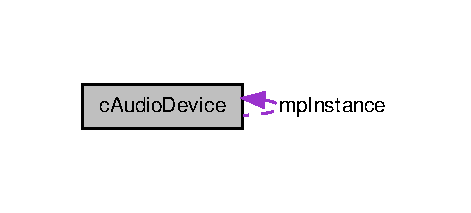
\includegraphics[width=226pt]{classc_audio_device__coll__graph}
\end{center}
\end{figure}
\subsection*{Public Member Functions}
\begin{DoxyCompactItemize}
\item 
\hypertarget{classc_audio_device_a66ac901442496247a1e9a9ea7ef44120}{
\hyperlink{classc_audio_device_a66ac901442496247a1e9a9ea7ef44120}{cAudioDevice} ()}
\label{classc_audio_device_a66ac901442496247a1e9a9ea7ef44120}

\begin{DoxyCompactList}\small\item\em Constructor will start and initialise an OpenAL system. \end{DoxyCompactList}\end{DoxyCompactItemize}
\subsection*{Static Public Member Functions}
\begin{DoxyCompactItemize}
\item 
\hypertarget{classc_audio_device_aebae28f8c27622a408e616c50e096e85}{
static \hyperlink{classc_audio_device}{cAudioDevice} $\ast$ \hyperlink{classc_audio_device_aebae28f8c27622a408e616c50e096e85}{Instance} ()}
\label{classc_audio_device_aebae28f8c27622a408e616c50e096e85}

\begin{DoxyCompactList}\small\item\em This Function will return a pointer to the current OpenAL Audio Device. \end{DoxyCompactList}\end{DoxyCompactItemize}


\subsection{Detailed Description}
This class will initialise the sound card. This class will initialise an audio device so sounds can be played on the system. 
\hypertarget{classc_audio_object}{
\section{cAudioObject Class Reference}
\label{classc_audio_object}\index{cAudioObject@{cAudioObject}}
}


This class will allow a sound to be played. This class will link an audio source and a buffer, This allows the sound data stored in the buffer to be played through the source. Each source is an audio channel and can only play one sound at a time.  




Collaboration diagram for cAudioObject:
\nopagebreak
\begin{figure}[H]
\begin{center}
\leavevmode
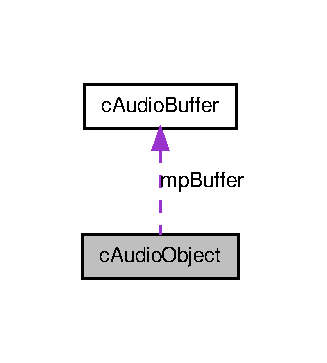
\includegraphics[width=157pt]{classc_audio_object__coll__graph}
\end{center}
\end{figure}
\subsection*{Public Member Functions}
\begin{DoxyCompactItemize}
\item 
\hyperlink{classc_audio_object_a1a44ae87c2bf5e43aff66624a42771fe}{cAudioObject} ()
\begin{DoxyCompactList}\small\item\em This will create an OpenAL source for this object, without linking any cAudioBuffers to it. \item\end{DoxyCompactList}\item 
\hyperlink{classc_audio_object_a172d5d9e89376a0c505fa051e9d02919}{cAudioObject} (\hyperlink{classc_audio_buffer}{cAudioBuffer} $\ast$lpBuffer)
\begin{DoxyCompactList}\small\item\em This will create an OpenAL source and link this object to a buffer. \item\end{DoxyCompactList}\item 
\hyperlink{classc_audio_object_a57baf1e1384c3307ce8db629c9b2a59f}{$\sim$cAudioObject} ()
\item 
void \hyperlink{classc_audio_object_aaa2c81875452c51ecd3979a0b1b2c8b1}{SetBuffer} (\hyperlink{classc_audio_buffer}{cAudioBuffer} $\ast$lpBuffer)
\begin{DoxyCompactList}\small\item\em This will link the OpenAL buffer pointed to by lpBuffer to this Audio Object ready to be played. \item\end{DoxyCompactList}\item 
void \hyperlink{classc_audio_object_a2e7c8dc824eef10006f0f1c2824f10cd}{Play} ()
\begin{DoxyCompactList}\small\item\em This will play a sound through the OpenAL source from the buffer. \item\end{DoxyCompactList}\item 
ALuint \hyperlink{classc_audio_object_adb134027851226f2f5a446a3d885f26e}{Source} ()
\begin{DoxyCompactList}\small\item\em This will return the ID of the OpenAL ID. \item\end{DoxyCompactList}\end{DoxyCompactItemize}


\subsection{Detailed Description}
This class will allow a sound to be played. This class will link an audio source and a buffer, This allows the sound data stored in the buffer to be played through the source. Each source is an audio channel and can only play one sound at a time. 

Definition at line 7 of file WTcAudioObject.h.



\subsection{Constructor \& Destructor Documentation}
\hypertarget{classc_audio_object_a1a44ae87c2bf5e43aff66624a42771fe}{
\index{cAudioObject@{cAudioObject}!cAudioObject@{cAudioObject}}
\index{cAudioObject@{cAudioObject}!cAudioObject@{cAudioObject}}
\subsubsection[{cAudioObject}]{\setlength{\rightskip}{0pt plus 5cm}cAudioObject::cAudioObject (
\begin{DoxyParamCaption}
{}
\end{DoxyParamCaption}
)}}
\label{classc_audio_object_a1a44ae87c2bf5e43aff66624a42771fe}


This will create an OpenAL source for this object, without linking any cAudioBuffers to it. 



Definition at line 3 of file WTcAudioObject.cpp.

\hypertarget{classc_audio_object_a172d5d9e89376a0c505fa051e9d02919}{
\index{cAudioObject@{cAudioObject}!cAudioObject@{cAudioObject}}
\index{cAudioObject@{cAudioObject}!cAudioObject@{cAudioObject}}
\subsubsection[{cAudioObject}]{\setlength{\rightskip}{0pt plus 5cm}cAudioObject::cAudioObject (
\begin{DoxyParamCaption}
\item[{{\bf cAudioBuffer} $\ast$}]{lpBuffer}
\end{DoxyParamCaption}
)}}
\label{classc_audio_object_a172d5d9e89376a0c505fa051e9d02919}


This will create an OpenAL source and link this object to a buffer. 



Definition at line 9 of file WTcAudioObject.cpp.

\hypertarget{classc_audio_object_a57baf1e1384c3307ce8db629c9b2a59f}{
\index{cAudioObject@{cAudioObject}!$\sim$cAudioObject@{$\sim$cAudioObject}}
\index{$\sim$cAudioObject@{$\sim$cAudioObject}!cAudioObject@{cAudioObject}}
\subsubsection[{$\sim$cAudioObject}]{\setlength{\rightskip}{0pt plus 5cm}cAudioObject::$\sim$cAudioObject (
\begin{DoxyParamCaption}
{}
\end{DoxyParamCaption}
)}}
\label{classc_audio_object_a57baf1e1384c3307ce8db629c9b2a59f}


Definition at line 17 of file WTcAudioObject.cpp.



\subsection{Member Function Documentation}
\hypertarget{classc_audio_object_a2e7c8dc824eef10006f0f1c2824f10cd}{
\index{cAudioObject@{cAudioObject}!Play@{Play}}
\index{Play@{Play}!cAudioObject@{cAudioObject}}
\subsubsection[{Play}]{\setlength{\rightskip}{0pt plus 5cm}void cAudioObject::Play (
\begin{DoxyParamCaption}
{}
\end{DoxyParamCaption}
)}}
\label{classc_audio_object_a2e7c8dc824eef10006f0f1c2824f10cd}


This will play a sound through the OpenAL source from the buffer. 



Definition at line 22 of file WTcAudioObject.cpp.

\hypertarget{classc_audio_object_aaa2c81875452c51ecd3979a0b1b2c8b1}{
\index{cAudioObject@{cAudioObject}!SetBuffer@{SetBuffer}}
\index{SetBuffer@{SetBuffer}!cAudioObject@{cAudioObject}}
\subsubsection[{SetBuffer}]{\setlength{\rightskip}{0pt plus 5cm}void cAudioObject::SetBuffer (
\begin{DoxyParamCaption}
\item[{{\bf cAudioBuffer} $\ast$}]{lpBuffer}
\end{DoxyParamCaption}
)}}
\label{classc_audio_object_aaa2c81875452c51ecd3979a0b1b2c8b1}


This will link the OpenAL buffer pointed to by lpBuffer to this Audio Object ready to be played. 



Definition at line 27 of file WTcAudioObject.cpp.

\hypertarget{classc_audio_object_adb134027851226f2f5a446a3d885f26e}{
\index{cAudioObject@{cAudioObject}!Source@{Source}}
\index{Source@{Source}!cAudioObject@{cAudioObject}}
\subsubsection[{Source}]{\setlength{\rightskip}{0pt plus 5cm}ALuint cAudioObject::Source (
\begin{DoxyParamCaption}
{}
\end{DoxyParamCaption}
)}}
\label{classc_audio_object_adb134027851226f2f5a446a3d885f26e}


This will return the ID of the OpenAL ID. 



Definition at line 35 of file WTcAudioObject.cpp.


\hypertarget{classc_beam_collision}{
\section{cBeamCollision Class Reference}
\label{classc_beam_collision}\index{cBeamCollision@{cBeamCollision}}
}


Collaboration diagram for cBeamCollision:\nopagebreak
\begin{figure}[H]
\begin{center}
\leavevmode
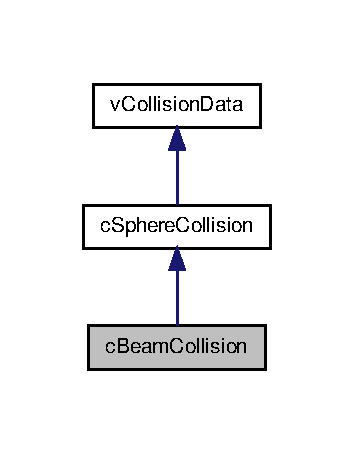
\includegraphics[width=170pt]{classc_beam_collision__coll__graph}
\end{center}
\end{figure}
\subsection*{Public Member Functions}
\begin{DoxyCompactItemize}
\item 
\hypertarget{classc_beam_collision_a8341836a9d69ea56fa119276b6ed29f4}{
void \hyperlink{classc_beam_collision_a8341836a9d69ea56fa119276b6ed29f4}{BuildObject} (float lfLength, float lfRadius)}
\label{classc_beam_collision_a8341836a9d69ea56fa119276b6ed29f4}

\begin{DoxyCompactList}\small\item\em This will generate a \hyperlink{classc_beam_collision}{cBeamCollision} data set of length lfength and Radius lfRadius. \end{DoxyCompactList}\item 
\hypertarget{classc_beam_collision_ae2cb900aab3fc1562c1162e6b5ab98f5}{
virtual \hyperlink{classc_beam_collision}{cBeamCollision} $\ast$ \hyperlink{classc_beam_collision_ae2cb900aab3fc1562c1162e6b5ab98f5}{Beam} ()}
\label{classc_beam_collision_ae2cb900aab3fc1562c1162e6b5ab98f5}

\begin{DoxyCompactList}\small\item\em Will return a pointer if this object contains a Beam collision data object. Otherwise returns 0;. \end{DoxyCompactList}\item 
\hypertarget{classc_beam_collision_a26f8662d41bc325dd14e3be9e7f1d1e9}{
virtual \hyperlink{classc_ray_collision}{cRayCollision} $\ast$ \hyperlink{classc_beam_collision_a26f8662d41bc325dd14e3be9e7f1d1e9}{Ray} ()}
\label{classc_beam_collision_a26f8662d41bc325dd14e3be9e7f1d1e9}

\begin{DoxyCompactList}\small\item\em Will return a pointer if this object contains a Ray collision data object. Otherwise returns 0;. \end{DoxyCompactList}\item 
\hypertarget{classc_beam_collision_a9c4fdda013d88c516edbb470ce9fab01}{
float $\ast$ \hyperlink{classc_beam_collision_a9c4fdda013d88c516edbb470ce9fab01}{RayVector} ()}
\label{classc_beam_collision_a9c4fdda013d88c516edbb470ce9fab01}

\begin{DoxyCompactList}\small\item\em Will return a float array with the beams global vector representing the direction it is pointing in. This should be normalised. \end{DoxyCompactList}\item 
\hypertarget{classc_beam_collision_a2eb26dfd4255ce8a2a10a7b142fb7f42}{
float \hyperlink{classc_beam_collision_a2eb26dfd4255ce8a2a10a7b142fb7f42}{Length} ()}
\label{classc_beam_collision_a2eb26dfd4255ce8a2a10a7b142fb7f42}

\begin{DoxyCompactList}\small\item\em Will return the length of the beam. \end{DoxyCompactList}\item 
\hypertarget{classc_beam_collision_ab7a645cc905fc9c62bfd6a1440d349b1}{
uint8 \hyperlink{classc_beam_collision_ab7a645cc905fc9c62bfd6a1440d349b1}{Type} ()}
\label{classc_beam_collision_ab7a645cc905fc9c62bfd6a1440d349b1}

\begin{DoxyCompactList}\small\item\em Will return the Objects Type. \end{DoxyCompactList}\end{DoxyCompactItemize}
\subsection*{Friends}
\begin{DoxyCompactItemize}
\item 
\hypertarget{classc_beam_collision_a70bfdc2c4682463db2e7755ec3e6440e}{
class \hyperlink{classc_beam_collision_a70bfdc2c4682463db2e7755ec3e6440e}{cMouse}}
\label{classc_beam_collision_a70bfdc2c4682463db2e7755ec3e6440e}

\end{DoxyCompactItemize}


\subsection{Detailed Description}
This class is for representing beams. Think energy beams. The system will assume that the object is a sphere of radius equal to the value set in SetSize(float $\ast$lfSize). The system will project the beam from the centrepoint of the beams current position in the direction of the Z-\/axis for a distance of mfLength. This is a fast and perfect (if the beam is a cylinder capped with hemi-\/spheres) way of colliding straight energy beams. See \hyperlink{classv_collision_data}{vCollisionData} for more information. 
\hypertarget{classc_beam_mesh}{
\section{cBeamMesh Class Reference}
\label{classc_beam_mesh}\index{cBeamMesh@{cBeamMesh}}
}


A Procedurally generated cylindrical Renderable Object. This class will generate a cylinder with specified dimensions and segments. The origin for the cylinder is in the radial center of one end of the cylinder.  




Collaboration diagram for cBeamMesh:\nopagebreak
\begin{figure}[H]
\begin{center}
\leavevmode
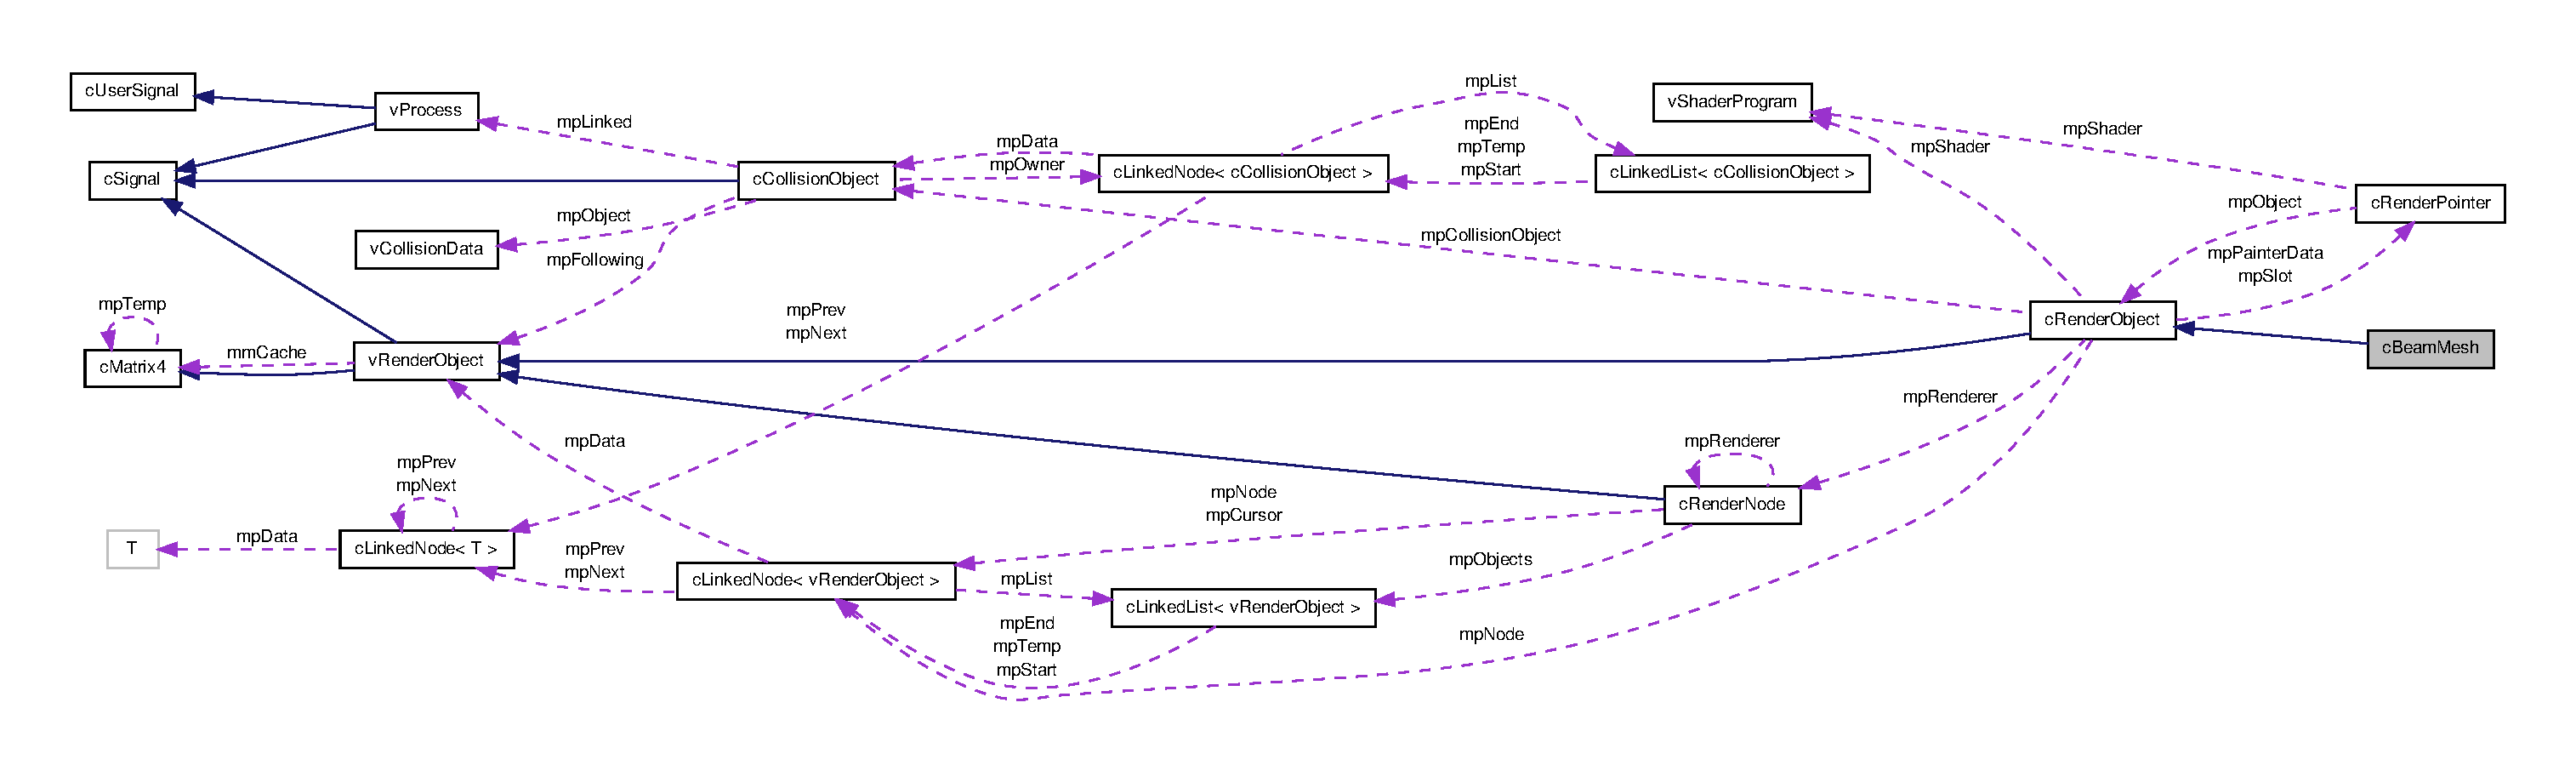
\includegraphics[width=400pt]{classc_beam_mesh__coll__graph}
\end{center}
\end{figure}
\subsection*{Public Member Functions}
\begin{DoxyCompactItemize}
\item 
\hypertarget{classc_beam_mesh_acf82cda9d282def977903ff877f36a26}{
\hyperlink{classc_beam_mesh_acf82cda9d282def977903ff877f36a26}{cBeamMesh} (float Radius=0.1f, float Length=1.0f, uint16 Segments=6, vRenderNode $\ast$lpNode=cCamera::Instance()-\/$>$RenderList())}
\label{classc_beam_mesh_acf82cda9d282def977903ff877f36a26}

\begin{DoxyCompactList}\small\item\em Constructor to Create a Beam with the specified Dimensions. Segments must be an even integer. \end{DoxyCompactList}\item 
\hypertarget{classc_beam_mesh_a1d2f2bfef0e3f96597ae6e1e73072030}{
void \hyperlink{classc_beam_mesh_a1d2f2bfef0e3f96597ae6e1e73072030}{Length} (float Length)}
\label{classc_beam_mesh_a1d2f2bfef0e3f96597ae6e1e73072030}

\begin{DoxyCompactList}\small\item\em Sets the Length of the Cylinder. \end{DoxyCompactList}\item 
\hypertarget{classc_beam_mesh_ac11934e813765321e76405cd96304088}{
void \hyperlink{classc_beam_mesh_ac11934e813765321e76405cd96304088}{Radius} (float Radius)}
\label{classc_beam_mesh_ac11934e813765321e76405cd96304088}

\begin{DoxyCompactList}\small\item\em Sets the Radius of the Cylinder. \end{DoxyCompactList}\item 
\hypertarget{classc_beam_mesh_ab59d3bb8c0a5c2944a206deaca3d2022}{
void \hyperlink{classc_beam_mesh_ab59d3bb8c0a5c2944a206deaca3d2022}{GenerateData} (float Radius, float Length, uint16 Segments)}
\label{classc_beam_mesh_ab59d3bb8c0a5c2944a206deaca3d2022}

\begin{DoxyCompactList}\small\item\em Will regenerate the cylinder with the specified Specifications. \end{DoxyCompactList}\item 
\hypertarget{classc_beam_mesh_aa4daa383162c2560c1c5ed47d22484e5}{
float \hyperlink{classc_beam_mesh_aa4daa383162c2560c1c5ed47d22484e5}{Length} ()}
\label{classc_beam_mesh_aa4daa383162c2560c1c5ed47d22484e5}

\begin{DoxyCompactList}\small\item\em Returns the current Length of the Cylinder. \end{DoxyCompactList}\item 
\hypertarget{classc_beam_mesh_a6068db701b4835449bd40a437e3ee908}{
float \hyperlink{classc_beam_mesh_a6068db701b4835449bd40a437e3ee908}{Radius} ()}
\label{classc_beam_mesh_a6068db701b4835449bd40a437e3ee908}

\begin{DoxyCompactList}\small\item\em Returns the current Radius of the Cylinder. \end{DoxyCompactList}\end{DoxyCompactItemize}


\subsection{Detailed Description}
A Procedurally generated cylindrical Renderable Object. This class will generate a cylinder with specified dimensions and segments. The origin for the cylinder is in the radial center of one end of the cylinder. 
\hypertarget{classc_camera}{
\section{cCamera Class Reference}
\label{classc_camera}\index{cCamera@{cCamera}}
}


This class will control the rendering of the render tree. It will handle all the render objects and how to render to the screen. \hyperlink{classc_camera}{cCamera} is the renderer for a single Render List. It will contain a scene graph, and inherits \hyperlink{classc_perspective_control}{cPerspectiveControl} and \hyperlink{classc_signal}{cSignal}. It also inherits \hyperlink{classc_viewport_control}{cViewportControl} and \hyperlink{classc_camera_matrix4}{cCameraMatrix4} through \hyperlink{classc_perspective_control}{cPerspectiveControl} It can be considered as a set of renderable objects with a camera, and will render every thing in its scene graph to the screen. It will not render any objects in another cCamera's scene graph. cRenderObjects and those inheriting it can be passed a \hyperlink{classc_camera}{cCamera} as a parameter on creation to make them exist in the camera. cViewports can be created which will render the same scene graph as their owning \hyperlink{classc_camera}{cCamera} object but from another perspective. The \hyperlink{classc_camera}{cCamera} object renders first, followed by the \hyperlink{classc_viewport}{cViewport} objects in the order they were created. \hyperlink{classc_camera}{cCamera} objects can be positioned and rotated using the functions in \hyperlink{classc_camera_matrix4}{cCameraMatrix4}. The region of the screen it renders to (the viewport) is set using the functions in \hyperlink{classc_viewport_control}{cViewportControl}. The perspective (field of view etc) is set by the functions in \hyperlink{classc_perspective_control}{cPerspectiveControl}.  




Collaboration diagram for cCamera:\nopagebreak
\begin{figure}[H]
\begin{center}
\leavevmode
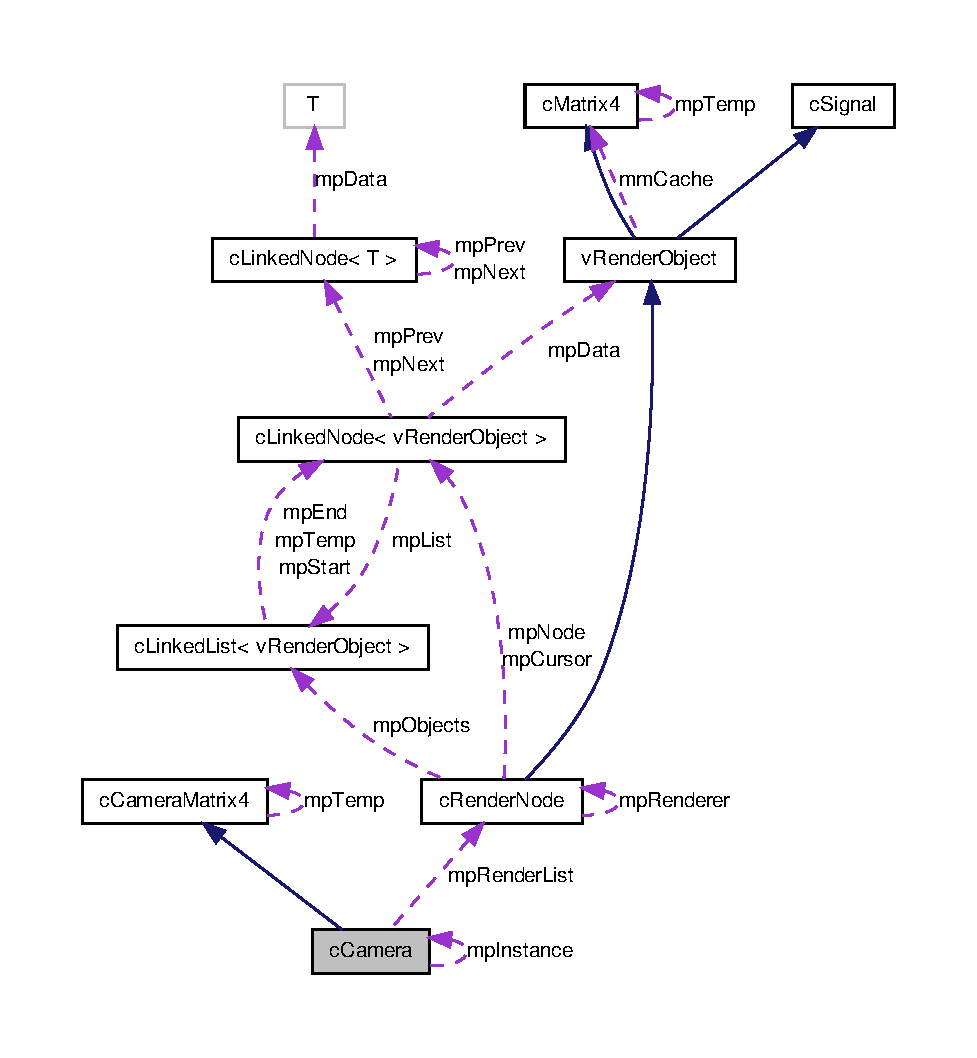
\includegraphics[width=400pt]{classc_camera__coll__graph}
\end{center}
\end{figure}
\subsection*{Public Member Functions}
\begin{DoxyCompactItemize}
\item 
\hypertarget{classc_camera_a1dbeb4e752d2a4cb50073a43c8c2132f}{
void \hyperlink{classc_camera_a1dbeb4e752d2a4cb50073a43c8c2132f}{RecalculateTotalMatrices} ()}
\label{classc_camera_a1dbeb4e752d2a4cb50073a43c8c2132f}

\begin{DoxyCompactList}\small\item\em Will recalculate all the total matrices (Projection$\ast$Camera$\ast$Global) in \hyperlink{classc_render_object}{cRenderObject} objects in this \hyperlink{classc_camera}{cCamera} objects render tree. \end{DoxyCompactList}\item 
\hypertarget{classc_camera_a4b27d2d3296c628615dc06b312459d70}{
void \hyperlink{classc_camera_a4b27d2d3296c628615dc06b312459d70}{RecalculateAllMatrices} ()}
\label{classc_camera_a4b27d2d3296c628615dc06b312459d70}

\begin{DoxyCompactList}\small\item\em Will recalculate all teh matrices in \hyperlink{classc_render_object}{cRenderObject} objects in this \hyperlink{classc_camera}{cCamera} objects render tree. \end{DoxyCompactList}\item 
\hypertarget{classc_camera_a9f2dcf74c52d7d3d0f4199b9e0d491c6}{
\hyperlink{classc_render_node}{cRenderNode} $\ast$ \hyperlink{classc_camera_a9f2dcf74c52d7d3d0f4199b9e0d491c6}{RenderList} ()}
\label{classc_camera_a9f2dcf74c52d7d3d0f4199b9e0d491c6}

\begin{DoxyCompactList}\small\item\em This will return a pointer to the scene graph. \end{DoxyCompactList}\item 
\hypertarget{classc_camera_ac63b2c284eee4b9b7182d85390279336}{
vRenderObject $\ast$ \hyperlink{classc_camera_ac63b2c284eee4b9b7182d85390279336}{vRenderList} ()}
\label{classc_camera_ac63b2c284eee4b9b7182d85390279336}

\begin{DoxyCompactList}\small\item\em This will return a virtual pointer to the the scene graph. \end{DoxyCompactList}\item 
\hypertarget{classc_camera_a6701644b2d73e607cee85dbc866ba6d9}{
void \hyperlink{classc_camera_a6701644b2d73e607cee85dbc866ba6d9}{Stop} ()}
\label{classc_camera_a6701644b2d73e607cee85dbc866ba6d9}

\begin{DoxyCompactList}\small\item\em Function for performing \hyperlink{classc_camera}{cCamera} specific actions after receiving a kill signal from via \hyperlink{classc_signal_a545074be1da41d00050bed3cd2fb2305}{cSignal::Signal(SIGNAL)}. \end{DoxyCompactList}\item 
\hypertarget{classc_camera_ab798297d6aa91192e45f7910da1e0f9b}{
\hyperlink{classc_particle_handler}{cParticleHandler} $\ast$ \hyperlink{classc_camera_ab798297d6aa91192e45f7910da1e0f9b}{ParticleHandler} ()}
\label{classc_camera_ab798297d6aa91192e45f7910da1e0f9b}

\begin{DoxyCompactList}\small\item\em Function for returning a pointer to the \hyperlink{classc_particle_handler}{cParticleHandler} for this \hyperlink{classc_camera}{cCamera}. \end{DoxyCompactList}\end{DoxyCompactItemize}
\subsection*{Static Public Member Functions}
\begin{DoxyCompactItemize}
\item 
\hypertarget{classc_camera_a06efab78c09ce37c375837242719bf58}{
static \hyperlink{classc_camera}{cCamera} $\ast$ \hyperlink{classc_camera_a06efab78c09ce37c375837242719bf58}{Instance} ()}
\label{classc_camera_a06efab78c09ce37c375837242719bf58}

\begin{DoxyCompactList}\small\item\em This function will return a pointer to the first \hyperlink{classc_camera}{cCamera} object. This can be accessed by calling tjhe macro \_\-CAMERA. \end{DoxyCompactList}\end{DoxyCompactItemize}
\subsection*{Friends}
\begin{DoxyCompactItemize}
\item 
\hypertarget{classc_camera_a36b5bd53c16eecf39974e65e00bd408e}{
class \hyperlink{classc_camera_a36b5bd53c16eecf39974e65e00bd408e}{cViewport}}
\label{classc_camera_a36b5bd53c16eecf39974e65e00bd408e}

\end{DoxyCompactItemize}


\subsection{Detailed Description}
This class will control the rendering of the render tree. It will handle all the render objects and how to render to the screen. \hyperlink{classc_camera}{cCamera} is the renderer for a single Render List. It will contain a scene graph, and inherits \hyperlink{classc_perspective_control}{cPerspectiveControl} and \hyperlink{classc_signal}{cSignal}. It also inherits \hyperlink{classc_viewport_control}{cViewportControl} and \hyperlink{classc_camera_matrix4}{cCameraMatrix4} through \hyperlink{classc_perspective_control}{cPerspectiveControl} It can be considered as a set of renderable objects with a camera, and will render every thing in its scene graph to the screen. It will not render any objects in another cCamera's scene graph. cRenderObjects and those inheriting it can be passed a \hyperlink{classc_camera}{cCamera} as a parameter on creation to make them exist in the camera. cViewports can be created which will render the same scene graph as their owning \hyperlink{classc_camera}{cCamera} object but from another perspective. The \hyperlink{classc_camera}{cCamera} object renders first, followed by the \hyperlink{classc_viewport}{cViewport} objects in the order they were created. \hyperlink{classc_camera}{cCamera} objects can be positioned and rotated using the functions in \hyperlink{classc_camera_matrix4}{cCameraMatrix4}. The region of the screen it renders to (the viewport) is set using the functions in \hyperlink{classc_viewport_control}{cViewportControl}. The perspective (field of view etc) is set by the functions in \hyperlink{classc_perspective_control}{cPerspectiveControl}. 
\hypertarget{classc_camera_matrix4}{
\section{cCameraMatrix4 Class Reference}
\label{classc_camera_matrix4}\index{cCameraMatrix4@{cCameraMatrix4}}
}


This is a translation matrix for a camera object. This is a translation matrix for a camera. All the translations are inverted. Distances are 'reversed', Local rotations are 'globalised' and Global roatations are 'localised'. Effectively all the translations are inverted before they are applied to this matrix.  




Inheritance diagram for cCameraMatrix4:
\nopagebreak
\begin{figure}[H]
\begin{center}
\leavevmode
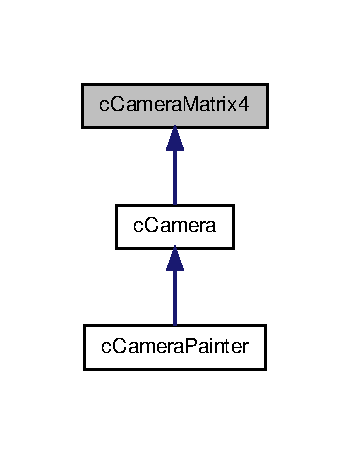
\includegraphics[width=168pt]{classc_camera_matrix4__inherit__graph}
\end{center}
\end{figure}


Collaboration diagram for cCameraMatrix4:
\nopagebreak
\begin{figure}[H]
\begin{center}
\leavevmode
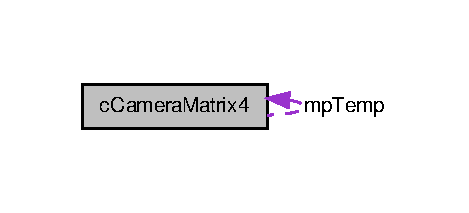
\includegraphics[width=225pt]{classc_camera_matrix4__coll__graph}
\end{center}
\end{figure}
\subsection*{Public Member Functions}
\begin{DoxyCompactItemize}
\item 
\hyperlink{classc_camera_matrix4_a99df6d312702e5474c5fedad42c95026}{cCameraMatrix4} ()
\begin{DoxyCompactList}\small\item\em This will create this matrix, and initialise all the static data for operations. \item\end{DoxyCompactList}\item 
float \hyperlink{classc_camera_matrix4_a4f3456fc67fbd37692a8daa9d11d5fc6}{Determinant} ()
\begin{DoxyCompactList}\small\item\em This will return the determinant of this matrix. \item\end{DoxyCompactList}\item 
\hyperlink{classc_camera_matrix4}{cCameraMatrix4} \hyperlink{classc_camera_matrix4_ac1fa4dd9add669a8faecd0ca79713278}{Transpose} ()
\begin{DoxyCompactList}\small\item\em This will return the transpose of this objects matrix ready for multiplications etc. \item\end{DoxyCompactList}\item 
void \hyperlink{classc_camera_matrix4_a97d111c444dd87ecec278e585fe058a7}{InvSign} ()
\begin{DoxyCompactList}\small\item\em This will make all terms of the matrix, the opposite sign to what they area. \item\end{DoxyCompactList}\item 
float $\ast$ \hyperlink{classc_camera_matrix4_ad8aad043cd8c21d5323b56cbcc90ef78}{Matrix} ()
\begin{DoxyCompactList}\small\item\em This will return a pointer to this objects matrix. \item\end{DoxyCompactList}\item 
float $\ast$ \hyperlink{classc_camera_matrix4_a89fba901320f6dda9a6b92bac09db915}{Position} ()
\begin{DoxyCompactList}\small\item\em This will return the position vector of this objects matrix. \item\end{DoxyCompactList}\item 
float \hyperlink{classc_camera_matrix4_a0133c16b734fa93e767ea89964799fb5}{X} ()
\begin{DoxyCompactList}\small\item\em This will return the X position of this objects matrix. \item\end{DoxyCompactList}\item 
float \hyperlink{classc_camera_matrix4_aec72cb78c62b2e0970824262b0b4aa1f}{Y} ()
\begin{DoxyCompactList}\small\item\em This will return the Y position of this objects matrix. \item\end{DoxyCompactList}\item 
float \hyperlink{classc_camera_matrix4_a7e3030fcedbd3b74270b26ea2b61904c}{Z} ()
\begin{DoxyCompactList}\small\item\em This will return the Z position of this objects matrix. \item\end{DoxyCompactList}\item 
void \hyperlink{classc_camera_matrix4_a23a05c1aff8a58dc662f5b871b422c17}{Identity} ()
\begin{DoxyCompactList}\small\item\em This will restore this objects matrix to an Identity matrix. \item\end{DoxyCompactList}\item 
void \hyperlink{classc_camera_matrix4_a1ec81a7ec3274f89d2b8fb94923345c0}{Zero} ()
\begin{DoxyCompactList}\small\item\em This will make the entire objects matrix equal to zero. \item\end{DoxyCompactList}\item 
\hyperlink{classc_camera_matrix4}{cCameraMatrix4} \hyperlink{classc_camera_matrix4_a975232c74548b9af68354bf6c19351d8}{operator$\ast$} (float \&lVal)
\begin{DoxyCompactList}\small\item\em This will multiplty the matrix by a float. \item\end{DoxyCompactList}\item 
\hyperlink{classc_camera_matrix4}{cCameraMatrix4} \hyperlink{classc_camera_matrix4_a41e56ee4a22ed37543c120d663e4bc3c}{operator$\ast$} (const float lVal)
\begin{DoxyCompactList}\small\item\em This will multiplty the matrix by a float. \item\end{DoxyCompactList}\item 
\hyperlink{classc_camera_matrix4}{cCameraMatrix4} \hyperlink{classc_camera_matrix4_ac3ca3f392c5046dd428cfe8cde194d37}{operator$\ast$} (\hyperlink{classc_camera_matrix4}{cCameraMatrix4} \&lVal)
\begin{DoxyCompactList}\small\item\em This will multiply this matrix by the matrix lVal. \item\end{DoxyCompactList}\item 
\hyperlink{classc_camera_matrix4}{cCameraMatrix4} $\ast$ \hyperlink{classc_camera_matrix4_a67a5947084f07eae0dd698477e1a7689}{operator$\ast$} (\hyperlink{classc_camera_matrix4}{cCameraMatrix4} $\ast$lVal)
\begin{DoxyCompactList}\small\item\em This will multiply this matrix by the matrix pointed to by lVal. \item\end{DoxyCompactList}\item 
\hyperlink{classc_camera_matrix4}{cCameraMatrix4} \hyperlink{classc_camera_matrix4_a71c4f0d6ee680f0cd511354de0033c64}{operator/} (float \&lVal)
\begin{DoxyCompactList}\small\item\em This will devide this objects matrix by the float lVal. \item\end{DoxyCompactList}\item 
\hyperlink{classc_camera_matrix4}{cCameraMatrix4} \hyperlink{classc_camera_matrix4_ab8d3c0c3df306102db000c37323692a3}{operator/} (const float lVal)
\begin{DoxyCompactList}\small\item\em This will devide this objects matrix by the float lVal. \item\end{DoxyCompactList}\item 
\hyperlink{classc_camera_matrix4}{cCameraMatrix4} \hyperlink{classc_camera_matrix4_a97ada5a5b0698d4e8f383754f30cbd2b}{operator+} (float \&lVal)
\begin{DoxyCompactList}\small\item\em This will add lVal to this objects matrix. lVal is added to every position in the matrix. \item\end{DoxyCompactList}\item 
\hyperlink{classc_camera_matrix4}{cCameraMatrix4} \hyperlink{classc_camera_matrix4_adb619821208a735d6fd262770d0dbf8a}{operator+} (const float lVal)
\begin{DoxyCompactList}\small\item\em This will add lVal to this objects matrix. lVal is added to every position in the matrix. \item\end{DoxyCompactList}\item 
\hyperlink{classc_camera_matrix4}{cCameraMatrix4} \hyperlink{classc_camera_matrix4_a4456564f6c57e7a9072ab31c242bef49}{operator+} (\hyperlink{classc_camera_matrix4}{cCameraMatrix4} \&lVal)
\begin{DoxyCompactList}\small\item\em This will add this objects matrix and the matrix lVal. \item\end{DoxyCompactList}\item 
\hyperlink{classc_camera_matrix4}{cCameraMatrix4} \hyperlink{classc_camera_matrix4_a42eb30055c9b58f2fc3fabf8201e7929}{operator-\/} (float \&lVal)
\begin{DoxyCompactList}\small\item\em This will deduct lVal from this objects matrix. lVal is deducted from every position in the matrix. \item\end{DoxyCompactList}\item 
\hyperlink{classc_camera_matrix4}{cCameraMatrix4} \hyperlink{classc_camera_matrix4_a3f13c8e5f71d9c158332fe87a49f1b61}{operator-\/} (const float lVal)
\begin{DoxyCompactList}\small\item\em This will deduct lVal from this objects matrix. lVal is deducted from every position in the matrix. \item\end{DoxyCompactList}\item 
\hyperlink{classc_camera_matrix4}{cCameraMatrix4} \hyperlink{classc_camera_matrix4_a97c7f6820b87ea9a217c4412e0c89e49}{operator-\/} (\hyperlink{classc_camera_matrix4}{cCameraMatrix4} \&lVal)
\begin{DoxyCompactList}\small\item\em This will deduct the matrix lVal from this objects matrix. \item\end{DoxyCompactList}\item 
float \& \hyperlink{classc_camera_matrix4_a57bce39e1e5ff464edd9dd1c32fcdd3b}{operator\mbox{[}$\,$\mbox{]}} (uint16 liPos)
\begin{DoxyCompactList}\small\item\em This will return the float in the position liPos in this objects matrix. \item\end{DoxyCompactList}\item 
float \& \hyperlink{classc_camera_matrix4_aeae4d353c1153e9eb15461eac399a29f}{operator()} (uint16 liColumn, uint16 liRow)
\begin{DoxyCompactList}\small\item\em This will return the float in the position \mbox{[}liColumn,liRow\mbox{]} in this objects matrix. \item\end{DoxyCompactList}\item 
float \hyperlink{classc_camera_matrix4_a21020ff4493a379b107a98c8a699d5f7}{operator=} (float \&lVal)
\begin{DoxyCompactList}\small\item\em This will set every float in this objects matrix to lVal. \item\end{DoxyCompactList}\item 
float \hyperlink{classc_camera_matrix4_a13c2e801ef13951525908a0985cf2ba7}{operator=} (const float lVal)
\begin{DoxyCompactList}\small\item\em This will set every float in this objects matrix to lVal. \item\end{DoxyCompactList}\item 
\hyperlink{classc_camera_matrix4}{cCameraMatrix4} \hyperlink{classc_camera_matrix4_a570900cf46a3c6e8a31e957a4dd24103}{operator=} (\hyperlink{classc_camera_matrix4}{cCameraMatrix4} \&lVal)
\begin{DoxyCompactList}\small\item\em This will set this objects matrix to be the same as the matrix lVal. \item\end{DoxyCompactList}\item 
\hyperlink{classc_camera_matrix4}{cCameraMatrix4} $\ast$ \hyperlink{classc_camera_matrix4_aabdb9adddb777e59ae8594cb62b0e02e}{operator=} (\hyperlink{classc_camera_matrix4}{cCameraMatrix4} $\ast$lVal)
\begin{DoxyCompactList}\small\item\em This will set this objects matrix to be the same as the matrix lVal. \item\end{DoxyCompactList}\item 
void \hyperlink{classc_camera_matrix4_a62fa2879539cc733e661d02b8a898578}{Position} (\hyperlink{classc2_d_vf}{c2DVf} $\ast$lpPosition)
\begin{DoxyCompactList}\small\item\em This will set this objects matrix position (2D -\/ X,Y) vector to be the same as lpPosition. \item\end{DoxyCompactList}\item 
void \hyperlink{classc_camera_matrix4_a293ac7d2919eae7205b568ea56fa104c}{Position} (float lfX, float lfY)
\begin{DoxyCompactList}\small\item\em This will set this objects matrix position vector to be lfX,lfY. \item\end{DoxyCompactList}\item 
void \hyperlink{classc_camera_matrix4_a7110b0f3aa924a2cfefe8ca149e0b41f}{Position} (\hyperlink{classc3_d_vf}{c3DVf} $\ast$lpPosition)
\begin{DoxyCompactList}\small\item\em This will set this objects matrix position vector to be the same as lpPosition. \item\end{DoxyCompactList}\item 
void \hyperlink{classc_camera_matrix4_a1aa471464a30ce27fe339b743b840516}{Position} (float lfX, float lfY, float lfZ)
\begin{DoxyCompactList}\small\item\em This will set this objects matrix position vector to be lfX,lfY,lfZ. \item\end{DoxyCompactList}\item 
void \hyperlink{classc_camera_matrix4_af130ddef040458f01b9a2365f41c567a}{PositionX} (float lfX)
\begin{DoxyCompactList}\small\item\em This will set this objects X position to he lfX. \item\end{DoxyCompactList}\item 
void \hyperlink{classc_camera_matrix4_adce3f6365faf3af907994f50c004c736}{PositionY} (float lfY)
\begin{DoxyCompactList}\small\item\em This will set this objects Y position to he lfY. \item\end{DoxyCompactList}\item 
void \hyperlink{classc_camera_matrix4_a6ea814a92ce2d7fcc1ba66490127b2f2}{PositionZ} (float lfZ)
\begin{DoxyCompactList}\small\item\em This will set this objects Z position to he lfZ. \item\end{DoxyCompactList}\item 
void \hyperlink{classc_camera_matrix4_a4a07cdf5cb578378193487a1ac304380}{AdvanceX} (float lfDistance)
\begin{DoxyCompactList}\small\item\em This will advance the position of this objects X position by lfDistance along local axis. \item\end{DoxyCompactList}\item 
void \hyperlink{classc_camera_matrix4_a1c644144c6673fad0d45ac2a28065edb}{AdvanceY} (float lfDistance)
\begin{DoxyCompactList}\small\item\em This will advance the position of this objects Y position by lfDistance along local axis. \item\end{DoxyCompactList}\item 
void \hyperlink{classc_camera_matrix4_a18915056c461b31b5ea916715fa2582f}{AdvanceZ} (float lfDistance)
\begin{DoxyCompactList}\small\item\em This will advance the position of this objects Z position by lfDistance along local axis. \item\end{DoxyCompactList}\item 
void \hyperlink{classc_camera_matrix4_acd0e691c270f18c80965bf8da4442d5b}{Advance} (float lfX, float lfY, float lfZ)
\begin{DoxyCompactList}\small\item\em This will advance the position of this objects X,Y and Z positions by lfX,lfY and lfZ along local axis. \item\end{DoxyCompactList}\item 
void \hyperlink{classc_camera_matrix4_a69ef5c53bd239d2f1041ac9330c2cc08}{GAdvanceX} (float lfDistance)
\begin{DoxyCompactList}\small\item\em This will advance the position of this objects X position by lfDistance along global axis. \item\end{DoxyCompactList}\item 
void \hyperlink{classc_camera_matrix4_a7cb5d64085acdcc74dcad1e965a52b3b}{GAdvanceY} (float lfDistance)
\begin{DoxyCompactList}\small\item\em This will advance the position of this objects Y position by lfDistance along global axis. \item\end{DoxyCompactList}\item 
void \hyperlink{classc_camera_matrix4_afd68814e78dd2ffaec2f9bc4289aca36}{GAdvanceZ} (float lfDistance)
\begin{DoxyCompactList}\small\item\em This will advance the position of this objects Z position by lfDistance along global axis. \item\end{DoxyCompactList}\item 
void \hyperlink{classc_camera_matrix4_a342b888f43a65b6c4a14b818c2519157}{GAdvance} (float lfX, float lfY, float lfZ)
\begin{DoxyCompactList}\small\item\em This will advance the position of this objects X,Y and Z positions by lfX,lfY and lfZ along global axis. \item\end{DoxyCompactList}\item 
void \hyperlink{classc_camera_matrix4_ab9ea2ea9b429824586d4fa74e709426e}{LRotate} (float lfAngle)
\begin{DoxyCompactList}\small\item\em This will localy rotate the object by lfAngle radians about the Z axis. This is suitable to be used by 2D objects. \item\end{DoxyCompactList}\item 
void \hyperlink{classc_camera_matrix4_a08ffa3e8e4622821ba80aaa51300e645}{LRotateX} (float lfAngle)
\begin{DoxyCompactList}\small\item\em This will rotate the object by lfAngle radians about its local X axis. This is suitable for use by 3D objects. \item\end{DoxyCompactList}\item 
void \hyperlink{classc_camera_matrix4_a369f1a97e289850afffd03302bb5bd0f}{LRotateY} (float lfAngle)
\begin{DoxyCompactList}\small\item\em This will rotate the object by lfAngle radians about its local Y axis. This is suitable for use by 3D objects. \item\end{DoxyCompactList}\item 
void \hyperlink{classc_camera_matrix4_ad4574f0b96ef29472ca6a286f4d8204d}{LRotateZ} (float lfAngle)
\begin{DoxyCompactList}\small\item\em This will rotate the object by lfAngle radians about its local Z axis. This is suitable for use by 3D objects. \item\end{DoxyCompactList}\item 
void \hyperlink{classc_camera_matrix4_a09c8d44629bf63643c8f09ccdc2294bc}{GRotateX} (float lfAngle)
\begin{DoxyCompactList}\small\item\em This will rotate the object by lfAngle radians about its global X axis. This is suitable for use by 3D objects. \item\end{DoxyCompactList}\item 
void \hyperlink{classc_camera_matrix4_a48eb5374c0e7fa4eca25f48a6411052d}{GRotateY} (float lfAngle)
\begin{DoxyCompactList}\small\item\em This will rotate the object by lfAngle radians about its global Y axis. This is suitable for use by 3D objects. \item\end{DoxyCompactList}\item 
void \hyperlink{classc_camera_matrix4_a993d7410719b1fd7d871f728527a3947}{GRotateZ} (float lfAngle)
\begin{DoxyCompactList}\small\item\em This will rotate the object by lfAngle radians about its global Z axis. This is suitable for use by 3D objects. \item\end{DoxyCompactList}\item 
void \hyperlink{classc_camera_matrix4_a2fc16f6a7aa3ffec1317f71645aa857b}{GRotateX} (float lfAngle, float lfX, float lfY, float lfZ)
\begin{DoxyCompactList}\small\item\em This will rotate the object by lfAngle radians about the global X axis of the point lfX,lfY,lfZ. This is suitable for use by 3D objects. \item\end{DoxyCompactList}\item 
void \hyperlink{classc_camera_matrix4_a775326e51bf492340e8768d219a4e5e2}{GRotateY} (float lfAngle, float lfX, float lfY, float lfZ)
\begin{DoxyCompactList}\small\item\em This will rotate the object by lfAngle radians about the global Y axis of the point lfX,lfY,lfZ. This is suitable for use by 3D objects. \item\end{DoxyCompactList}\item 
void \hyperlink{classc_camera_matrix4_a8c99ce20f8594e9a66e0a7b2830ec9e9}{GRotateZ} (float lfAngle, float lfX, float lfY, float lfZ)
\begin{DoxyCompactList}\small\item\em This will rotate the object by lfAngle radians about the global Z axis of the point lfX,lfY,lfZ. This is suitable for use by 3D objects. \item\end{DoxyCompactList}\item 
void \hyperlink{classc_camera_matrix4_a6be0f1f82cc4ee5a5953cb3b569b4285}{Angle} (float lfAngle)
\begin{DoxyCompactList}\small\item\em This will set the current objects matrix to be rotated to the absolute angle lfAngle. This is suitable for 2D objects. \item\end{DoxyCompactList}\item 
void \hyperlink{classc_camera_matrix4_a620ba52edfd711f011d43a441eece9bc}{Resize} (float lfScale)
\begin{DoxyCompactList}\small\item\em This will scale this objects matrix by a factor of lfScale. \item\end{DoxyCompactList}\item 
void \hyperlink{classc_camera_matrix4_a53c3d81781d403c9bf9671879f79a838}{LResizeX} (float lfScale)
\begin{DoxyCompactList}\small\item\em This will scale this objects local X axis by a factor of lfScale. \item\end{DoxyCompactList}\item 
void \hyperlink{classc_camera_matrix4_a12eda8948b16c1a2818093016d8ef755}{LResizeY} (float lfScale)
\begin{DoxyCompactList}\small\item\em This will scale this objects local Y axis by a factor of lfScale. \item\end{DoxyCompactList}\item 
void \hyperlink{classc_camera_matrix4_a6f1fbcfe585f86002cb586eab9df7c7d}{LResizeZ} (float lfScale)
\begin{DoxyCompactList}\small\item\em This will scale this objects local Z axis by a factor of lfScale. \item\end{DoxyCompactList}\item 
void \hyperlink{classc_camera_matrix4_a9984a8427cd90e77a2fb6462ecf99ecc}{GResizeX} (float lfScale)
\begin{DoxyCompactList}\small\item\em This will scale this objects globally along the X axis by a factor of lfScale. \item\end{DoxyCompactList}\item 
void \hyperlink{classc_camera_matrix4_aa2a9326b7f2a6f00aa5b45057c69ecd3}{GResizeY} (float lfScale)
\begin{DoxyCompactList}\small\item\em This will scale this objects globally along the Y axis by a factor of lfScale. \item\end{DoxyCompactList}\item 
void \hyperlink{classc_camera_matrix4_a1ab7808cf06ddf7ec373b926c77f85c6}{GResizeZ} (float lfScale)
\begin{DoxyCompactList}\small\item\em This will scale this objects globally along the Z axis by a factor of lfScale. \item\end{DoxyCompactList}\item 
uint32 \hyperlink{classc_camera_matrix4_adf5481b8c761008b9611e0b071e70914}{Distance3D} (float $\ast$lpOther)
\begin{DoxyCompactList}\small\item\em This will return the 3D distance between this matrix and the matrix pointed to by lpOther. \item\end{DoxyCompactList}\item 
uint32 \hyperlink{classc_camera_matrix4_a02c68197ed3c64c95985269f5b9f66a4}{Distance2D} (float $\ast$lpOther)
\begin{DoxyCompactList}\small\item\em This will return the 2D distance between this matrix and the matrix pointed to by lpOther. \item\end{DoxyCompactList}\item 
void \hyperlink{classc_camera_matrix4_aeee787e0f5895a613e8be9efbade408f}{Follow} (\hyperlink{classc_matrix4}{cMatrix4} $\ast$lpOther, float lfDist)
\item 
void \hyperlink{classc_camera_matrix4_aa8ca47d59f6b3b454d700329bdbbdeea}{PointAt} (float $\ast$mpPos)
\end{DoxyCompactItemize}
\subsection*{Public Attributes}
\begin{DoxyCompactItemize}
\item 
float \hyperlink{classc_camera_matrix4_afb48ac51e480abcece16e031d8bc300a}{mpPosition} \mbox{[}3\mbox{]}
\begin{DoxyCompactList}\small\item\em The position of this matrix has been seperated from the rest of the matrix as the camera should rotate around 0,0,0, not itself? \item\end{DoxyCompactList}\end{DoxyCompactItemize}


\subsection{Detailed Description}
This is a translation matrix for a camera object. This is a translation matrix for a camera. All the translations are inverted. Distances are 'reversed', Local rotations are 'globalised' and Global roatations are 'localised'. Effectively all the translations are inverted before they are applied to this matrix. 

Definition at line 10 of file WTcCameraMatrix4.h.



\subsection{Constructor \& Destructor Documentation}
\hypertarget{classc_camera_matrix4_a99df6d312702e5474c5fedad42c95026}{
\index{cCameraMatrix4@{cCameraMatrix4}!cCameraMatrix4@{cCameraMatrix4}}
\index{cCameraMatrix4@{cCameraMatrix4}!cCameraMatrix4@{cCameraMatrix4}}
\subsubsection[{cCameraMatrix4}]{\setlength{\rightskip}{0pt plus 5cm}cCameraMatrix4::cCameraMatrix4 (
\begin{DoxyParamCaption}
{}
\end{DoxyParamCaption}
)}}
\label{classc_camera_matrix4_a99df6d312702e5474c5fedad42c95026}


This will create this matrix, and initialise all the static data for operations. 



Definition at line 9 of file WTcCameraMatrix4.cpp.



\subsection{Member Function Documentation}
\hypertarget{classc_camera_matrix4_acd0e691c270f18c80965bf8da4442d5b}{
\index{cCameraMatrix4@{cCameraMatrix4}!Advance@{Advance}}
\index{Advance@{Advance}!cCameraMatrix4@{cCameraMatrix4}}
\subsubsection[{Advance}]{\setlength{\rightskip}{0pt plus 5cm}void cCameraMatrix4::Advance (
\begin{DoxyParamCaption}
\item[{float}]{lfX, }
\item[{float}]{lfY, }
\item[{float}]{lfZ}
\end{DoxyParamCaption}
)}}
\label{classc_camera_matrix4_acd0e691c270f18c80965bf8da4442d5b}


This will advance the position of this objects X,Y and Z positions by lfX,lfY and lfZ along local axis. 



Definition at line 742 of file WTcCameraMatrix4.cpp.

\hypertarget{classc_camera_matrix4_a4a07cdf5cb578378193487a1ac304380}{
\index{cCameraMatrix4@{cCameraMatrix4}!AdvanceX@{AdvanceX}}
\index{AdvanceX@{AdvanceX}!cCameraMatrix4@{cCameraMatrix4}}
\subsubsection[{AdvanceX}]{\setlength{\rightskip}{0pt plus 5cm}void cCameraMatrix4::AdvanceX (
\begin{DoxyParamCaption}
\item[{float}]{lfDistance}
\end{DoxyParamCaption}
)}}
\label{classc_camera_matrix4_a4a07cdf5cb578378193487a1ac304380}


This will advance the position of this objects X position by lfDistance along local axis. 



Definition at line 720 of file WTcCameraMatrix4.cpp.

\hypertarget{classc_camera_matrix4_a1c644144c6673fad0d45ac2a28065edb}{
\index{cCameraMatrix4@{cCameraMatrix4}!AdvanceY@{AdvanceY}}
\index{AdvanceY@{AdvanceY}!cCameraMatrix4@{cCameraMatrix4}}
\subsubsection[{AdvanceY}]{\setlength{\rightskip}{0pt plus 5cm}void cCameraMatrix4::AdvanceY (
\begin{DoxyParamCaption}
\item[{float}]{lfDistance}
\end{DoxyParamCaption}
)}}
\label{classc_camera_matrix4_a1c644144c6673fad0d45ac2a28065edb}


This will advance the position of this objects Y position by lfDistance along local axis. 



Definition at line 727 of file WTcCameraMatrix4.cpp.

\hypertarget{classc_camera_matrix4_a18915056c461b31b5ea916715fa2582f}{
\index{cCameraMatrix4@{cCameraMatrix4}!AdvanceZ@{AdvanceZ}}
\index{AdvanceZ@{AdvanceZ}!cCameraMatrix4@{cCameraMatrix4}}
\subsubsection[{AdvanceZ}]{\setlength{\rightskip}{0pt plus 5cm}void cCameraMatrix4::AdvanceZ (
\begin{DoxyParamCaption}
\item[{float}]{lfDistance}
\end{DoxyParamCaption}
)}}
\label{classc_camera_matrix4_a18915056c461b31b5ea916715fa2582f}


This will advance the position of this objects Z position by lfDistance along local axis. 



Definition at line 734 of file WTcCameraMatrix4.cpp.

\hypertarget{classc_camera_matrix4_a6be0f1f82cc4ee5a5953cb3b569b4285}{
\index{cCameraMatrix4@{cCameraMatrix4}!Angle@{Angle}}
\index{Angle@{Angle}!cCameraMatrix4@{cCameraMatrix4}}
\subsubsection[{Angle}]{\setlength{\rightskip}{0pt plus 5cm}void cCameraMatrix4::Angle (
\begin{DoxyParamCaption}
\item[{float}]{lfAngle}
\end{DoxyParamCaption}
)}}
\label{classc_camera_matrix4_a6be0f1f82cc4ee5a5953cb3b569b4285}


This will set the current objects matrix to be rotated to the absolute angle lfAngle. This is suitable for 2D objects. 



Definition at line 513 of file WTcCameraMatrix4.cpp.

\hypertarget{classc_camera_matrix4_a4f3456fc67fbd37692a8daa9d11d5fc6}{
\index{cCameraMatrix4@{cCameraMatrix4}!Determinant@{Determinant}}
\index{Determinant@{Determinant}!cCameraMatrix4@{cCameraMatrix4}}
\subsubsection[{Determinant}]{\setlength{\rightskip}{0pt plus 5cm}float cCameraMatrix4::Determinant (
\begin{DoxyParamCaption}
{}
\end{DoxyParamCaption}
)}}
\label{classc_camera_matrix4_a4f3456fc67fbd37692a8daa9d11d5fc6}


This will return the determinant of this matrix. 



Definition at line 350 of file WTcCameraMatrix4.cpp.

\hypertarget{classc_camera_matrix4_a02c68197ed3c64c95985269f5b9f66a4}{
\index{cCameraMatrix4@{cCameraMatrix4}!Distance2D@{Distance2D}}
\index{Distance2D@{Distance2D}!cCameraMatrix4@{cCameraMatrix4}}
\subsubsection[{Distance2D}]{\setlength{\rightskip}{0pt plus 5cm}uint32 cCameraMatrix4::Distance2D (
\begin{DoxyParamCaption}
\item[{float $\ast$}]{lpOther}
\end{DoxyParamCaption}
)}}
\label{classc_camera_matrix4_a02c68197ed3c64c95985269f5b9f66a4}


This will return the 2D distance between this matrix and the matrix pointed to by lpOther. 



Definition at line 861 of file WTcCameraMatrix4.cpp.

\hypertarget{classc_camera_matrix4_adf5481b8c761008b9611e0b071e70914}{
\index{cCameraMatrix4@{cCameraMatrix4}!Distance3D@{Distance3D}}
\index{Distance3D@{Distance3D}!cCameraMatrix4@{cCameraMatrix4}}
\subsubsection[{Distance3D}]{\setlength{\rightskip}{0pt plus 5cm}uint32 cCameraMatrix4::Distance3D (
\begin{DoxyParamCaption}
\item[{float $\ast$}]{lpOther}
\end{DoxyParamCaption}
)}}
\label{classc_camera_matrix4_adf5481b8c761008b9611e0b071e70914}


This will return the 3D distance between this matrix and the matrix pointed to by lpOther. 



Definition at line 852 of file WTcCameraMatrix4.cpp.

\hypertarget{classc_camera_matrix4_aeee787e0f5895a613e8be9efbade408f}{
\index{cCameraMatrix4@{cCameraMatrix4}!Follow@{Follow}}
\index{Follow@{Follow}!cCameraMatrix4@{cCameraMatrix4}}
\subsubsection[{Follow}]{\setlength{\rightskip}{0pt plus 5cm}void cCameraMatrix4::Follow (
\begin{DoxyParamCaption}
\item[{{\bf cMatrix4} $\ast$}]{lpOther, }
\item[{float}]{lfDist}
\end{DoxyParamCaption}
)}}
\label{classc_camera_matrix4_aeee787e0f5895a613e8be9efbade408f}


Definition at line 869 of file WTcCameraMatrix4.cpp.

\hypertarget{classc_camera_matrix4_a342b888f43a65b6c4a14b818c2519157}{
\index{cCameraMatrix4@{cCameraMatrix4}!GAdvance@{GAdvance}}
\index{GAdvance@{GAdvance}!cCameraMatrix4@{cCameraMatrix4}}
\subsubsection[{GAdvance}]{\setlength{\rightskip}{0pt plus 5cm}void cCameraMatrix4::GAdvance (
\begin{DoxyParamCaption}
\item[{float}]{lfX, }
\item[{float}]{lfY, }
\item[{float}]{lfZ}
\end{DoxyParamCaption}
)}}
\label{classc_camera_matrix4_a342b888f43a65b6c4a14b818c2519157}


This will advance the position of this objects X,Y and Z positions by lfX,lfY and lfZ along global axis. 



Definition at line 758 of file WTcCameraMatrix4.cpp.

\hypertarget{classc_camera_matrix4_a69ef5c53bd239d2f1041ac9330c2cc08}{
\index{cCameraMatrix4@{cCameraMatrix4}!GAdvanceX@{GAdvanceX}}
\index{GAdvanceX@{GAdvanceX}!cCameraMatrix4@{cCameraMatrix4}}
\subsubsection[{GAdvanceX}]{\setlength{\rightskip}{0pt plus 5cm}void cCameraMatrix4::GAdvanceX (
\begin{DoxyParamCaption}
\item[{float}]{lfDistance}
\end{DoxyParamCaption}
)}}
\label{classc_camera_matrix4_a69ef5c53bd239d2f1041ac9330c2cc08}


This will advance the position of this objects X position by lfDistance along global axis. 



Definition at line 749 of file WTcCameraMatrix4.cpp.

\hypertarget{classc_camera_matrix4_a7cb5d64085acdcc74dcad1e965a52b3b}{
\index{cCameraMatrix4@{cCameraMatrix4}!GAdvanceY@{GAdvanceY}}
\index{GAdvanceY@{GAdvanceY}!cCameraMatrix4@{cCameraMatrix4}}
\subsubsection[{GAdvanceY}]{\setlength{\rightskip}{0pt plus 5cm}void cCameraMatrix4::GAdvanceY (
\begin{DoxyParamCaption}
\item[{float}]{lfDistance}
\end{DoxyParamCaption}
)}}
\label{classc_camera_matrix4_a7cb5d64085acdcc74dcad1e965a52b3b}


This will advance the position of this objects Y position by lfDistance along global axis. 



Definition at line 752 of file WTcCameraMatrix4.cpp.

\hypertarget{classc_camera_matrix4_afd68814e78dd2ffaec2f9bc4289aca36}{
\index{cCameraMatrix4@{cCameraMatrix4}!GAdvanceZ@{GAdvanceZ}}
\index{GAdvanceZ@{GAdvanceZ}!cCameraMatrix4@{cCameraMatrix4}}
\subsubsection[{GAdvanceZ}]{\setlength{\rightskip}{0pt plus 5cm}void cCameraMatrix4::GAdvanceZ (
\begin{DoxyParamCaption}
\item[{float}]{lfDistance}
\end{DoxyParamCaption}
)}}
\label{classc_camera_matrix4_afd68814e78dd2ffaec2f9bc4289aca36}


This will advance the position of this objects Z position by lfDistance along global axis. 



Definition at line 755 of file WTcCameraMatrix4.cpp.

\hypertarget{classc_camera_matrix4_a9984a8427cd90e77a2fb6462ecf99ecc}{
\index{cCameraMatrix4@{cCameraMatrix4}!GResizeX@{GResizeX}}
\index{GResizeX@{GResizeX}!cCameraMatrix4@{cCameraMatrix4}}
\subsubsection[{GResizeX}]{\setlength{\rightskip}{0pt plus 5cm}void cCameraMatrix4::GResizeX (
\begin{DoxyParamCaption}
\item[{float}]{lfScale}
\end{DoxyParamCaption}
)}}
\label{classc_camera_matrix4_a9984a8427cd90e77a2fb6462ecf99ecc}


This will scale this objects globally along the X axis by a factor of lfScale. 



Definition at line 637 of file WTcCameraMatrix4.cpp.

\hypertarget{classc_camera_matrix4_aa2a9326b7f2a6f00aa5b45057c69ecd3}{
\index{cCameraMatrix4@{cCameraMatrix4}!GResizeY@{GResizeY}}
\index{GResizeY@{GResizeY}!cCameraMatrix4@{cCameraMatrix4}}
\subsubsection[{GResizeY}]{\setlength{\rightskip}{0pt plus 5cm}void cCameraMatrix4::GResizeY (
\begin{DoxyParamCaption}
\item[{float}]{lfScale}
\end{DoxyParamCaption}
)}}
\label{classc_camera_matrix4_aa2a9326b7f2a6f00aa5b45057c69ecd3}


This will scale this objects globally along the Y axis by a factor of lfScale. 



Definition at line 645 of file WTcCameraMatrix4.cpp.

\hypertarget{classc_camera_matrix4_a1ab7808cf06ddf7ec373b926c77f85c6}{
\index{cCameraMatrix4@{cCameraMatrix4}!GResizeZ@{GResizeZ}}
\index{GResizeZ@{GResizeZ}!cCameraMatrix4@{cCameraMatrix4}}
\subsubsection[{GResizeZ}]{\setlength{\rightskip}{0pt plus 5cm}void cCameraMatrix4::GResizeZ (
\begin{DoxyParamCaption}
\item[{float}]{lfScale}
\end{DoxyParamCaption}
)}}
\label{classc_camera_matrix4_a1ab7808cf06ddf7ec373b926c77f85c6}


This will scale this objects globally along the Z axis by a factor of lfScale. 



Definition at line 653 of file WTcCameraMatrix4.cpp.

\hypertarget{classc_camera_matrix4_a09c8d44629bf63643c8f09ccdc2294bc}{
\index{cCameraMatrix4@{cCameraMatrix4}!GRotateX@{GRotateX}}
\index{GRotateX@{GRotateX}!cCameraMatrix4@{cCameraMatrix4}}
\subsubsection[{GRotateX}]{\setlength{\rightskip}{0pt plus 5cm}void cCameraMatrix4::GRotateX (
\begin{DoxyParamCaption}
\item[{float}]{lfAngle}
\end{DoxyParamCaption}
)}}
\label{classc_camera_matrix4_a09c8d44629bf63643c8f09ccdc2294bc}


This will rotate the object by lfAngle radians about its global X axis. This is suitable for use by 3D objects. 



Definition at line 661 of file WTcCameraMatrix4.cpp.

\hypertarget{classc_camera_matrix4_a2fc16f6a7aa3ffec1317f71645aa857b}{
\index{cCameraMatrix4@{cCameraMatrix4}!GRotateX@{GRotateX}}
\index{GRotateX@{GRotateX}!cCameraMatrix4@{cCameraMatrix4}}
\subsubsection[{GRotateX}]{\setlength{\rightskip}{0pt plus 5cm}void cCameraMatrix4::GRotateX (
\begin{DoxyParamCaption}
\item[{float}]{lfAngle, }
\item[{float}]{lfX, }
\item[{float}]{lfY, }
\item[{float}]{lfZ}
\end{DoxyParamCaption}
)}}
\label{classc_camera_matrix4_a2fc16f6a7aa3ffec1317f71645aa857b}


This will rotate the object by lfAngle radians about the global X axis of the point lfX,lfY,lfZ. This is suitable for use by 3D objects. 



Definition at line 765 of file WTcCameraMatrix4.cpp.

\hypertarget{classc_camera_matrix4_a48eb5374c0e7fa4eca25f48a6411052d}{
\index{cCameraMatrix4@{cCameraMatrix4}!GRotateY@{GRotateY}}
\index{GRotateY@{GRotateY}!cCameraMatrix4@{cCameraMatrix4}}
\subsubsection[{GRotateY}]{\setlength{\rightskip}{0pt plus 5cm}void cCameraMatrix4::GRotateY (
\begin{DoxyParamCaption}
\item[{float}]{lfAngle}
\end{DoxyParamCaption}
)}}
\label{classc_camera_matrix4_a48eb5374c0e7fa4eca25f48a6411052d}


This will rotate the object by lfAngle radians about its global Y axis. This is suitable for use by 3D objects. 



Definition at line 681 of file WTcCameraMatrix4.cpp.

\hypertarget{classc_camera_matrix4_a775326e51bf492340e8768d219a4e5e2}{
\index{cCameraMatrix4@{cCameraMatrix4}!GRotateY@{GRotateY}}
\index{GRotateY@{GRotateY}!cCameraMatrix4@{cCameraMatrix4}}
\subsubsection[{GRotateY}]{\setlength{\rightskip}{0pt plus 5cm}void cCameraMatrix4::GRotateY (
\begin{DoxyParamCaption}
\item[{float}]{lfAngle, }
\item[{float}]{lfX, }
\item[{float}]{lfY, }
\item[{float}]{lfZ}
\end{DoxyParamCaption}
)}}
\label{classc_camera_matrix4_a775326e51bf492340e8768d219a4e5e2}


This will rotate the object by lfAngle radians about the global Y axis of the point lfX,lfY,lfZ. This is suitable for use by 3D objects. 



Definition at line 795 of file WTcCameraMatrix4.cpp.

\hypertarget{classc_camera_matrix4_a993d7410719b1fd7d871f728527a3947}{
\index{cCameraMatrix4@{cCameraMatrix4}!GRotateZ@{GRotateZ}}
\index{GRotateZ@{GRotateZ}!cCameraMatrix4@{cCameraMatrix4}}
\subsubsection[{GRotateZ}]{\setlength{\rightskip}{0pt plus 5cm}void cCameraMatrix4::GRotateZ (
\begin{DoxyParamCaption}
\item[{float}]{lfAngle}
\end{DoxyParamCaption}
)}}
\label{classc_camera_matrix4_a993d7410719b1fd7d871f728527a3947}


This will rotate the object by lfAngle radians about its global Z axis. This is suitable for use by 3D objects. 



Definition at line 702 of file WTcCameraMatrix4.cpp.

\hypertarget{classc_camera_matrix4_a8c99ce20f8594e9a66e0a7b2830ec9e9}{
\index{cCameraMatrix4@{cCameraMatrix4}!GRotateZ@{GRotateZ}}
\index{GRotateZ@{GRotateZ}!cCameraMatrix4@{cCameraMatrix4}}
\subsubsection[{GRotateZ}]{\setlength{\rightskip}{0pt plus 5cm}void cCameraMatrix4::GRotateZ (
\begin{DoxyParamCaption}
\item[{float}]{lfAngle, }
\item[{float}]{lfX, }
\item[{float}]{lfY, }
\item[{float}]{lfZ}
\end{DoxyParamCaption}
)}}
\label{classc_camera_matrix4_a8c99ce20f8594e9a66e0a7b2830ec9e9}


This will rotate the object by lfAngle radians about the global Z axis of the point lfX,lfY,lfZ. This is suitable for use by 3D objects. 



Definition at line 825 of file WTcCameraMatrix4.cpp.

\hypertarget{classc_camera_matrix4_a23a05c1aff8a58dc662f5b871b422c17}{
\index{cCameraMatrix4@{cCameraMatrix4}!Identity@{Identity}}
\index{Identity@{Identity}!cCameraMatrix4@{cCameraMatrix4}}
\subsubsection[{Identity}]{\setlength{\rightskip}{0pt plus 5cm}void cCameraMatrix4::Identity (
\begin{DoxyParamCaption}
{}
\end{DoxyParamCaption}
)}}
\label{classc_camera_matrix4_a23a05c1aff8a58dc662f5b871b422c17}


This will restore this objects matrix to an Identity matrix. 



Definition at line 302 of file WTcCameraMatrix4.cpp.

\hypertarget{classc_camera_matrix4_a97d111c444dd87ecec278e585fe058a7}{
\index{cCameraMatrix4@{cCameraMatrix4}!InvSign@{InvSign}}
\index{InvSign@{InvSign}!cCameraMatrix4@{cCameraMatrix4}}
\subsubsection[{InvSign}]{\setlength{\rightskip}{0pt plus 5cm}void cCameraMatrix4::InvSign (
\begin{DoxyParamCaption}
{}
\end{DoxyParamCaption}
)}}
\label{classc_camera_matrix4_a97d111c444dd87ecec278e585fe058a7}


This will make all terms of the matrix, the opposite sign to what they area. 



Definition at line 903 of file WTcCameraMatrix4.cpp.

\hypertarget{classc_camera_matrix4_a53c3d81781d403c9bf9671879f79a838}{
\index{cCameraMatrix4@{cCameraMatrix4}!LResizeX@{LResizeX}}
\index{LResizeX@{LResizeX}!cCameraMatrix4@{cCameraMatrix4}}
\subsubsection[{LResizeX}]{\setlength{\rightskip}{0pt plus 5cm}void cCameraMatrix4::LResizeX (
\begin{DoxyParamCaption}
\item[{float}]{lfScale}
\end{DoxyParamCaption}
)}}
\label{classc_camera_matrix4_a53c3d81781d403c9bf9671879f79a838}


This will scale this objects local X axis by a factor of lfScale. 



Definition at line 610 of file WTcCameraMatrix4.cpp.

\hypertarget{classc_camera_matrix4_a12eda8948b16c1a2818093016d8ef755}{
\index{cCameraMatrix4@{cCameraMatrix4}!LResizeY@{LResizeY}}
\index{LResizeY@{LResizeY}!cCameraMatrix4@{cCameraMatrix4}}
\subsubsection[{LResizeY}]{\setlength{\rightskip}{0pt plus 5cm}void cCameraMatrix4::LResizeY (
\begin{DoxyParamCaption}
\item[{float}]{lfScale}
\end{DoxyParamCaption}
)}}
\label{classc_camera_matrix4_a12eda8948b16c1a2818093016d8ef755}


This will scale this objects local Y axis by a factor of lfScale. 



Definition at line 618 of file WTcCameraMatrix4.cpp.

\hypertarget{classc_camera_matrix4_a6f1fbcfe585f86002cb586eab9df7c7d}{
\index{cCameraMatrix4@{cCameraMatrix4}!LResizeZ@{LResizeZ}}
\index{LResizeZ@{LResizeZ}!cCameraMatrix4@{cCameraMatrix4}}
\subsubsection[{LResizeZ}]{\setlength{\rightskip}{0pt plus 5cm}void cCameraMatrix4::LResizeZ (
\begin{DoxyParamCaption}
\item[{float}]{lfScale}
\end{DoxyParamCaption}
)}}
\label{classc_camera_matrix4_a6f1fbcfe585f86002cb586eab9df7c7d}


This will scale this objects local Z axis by a factor of lfScale. 



Definition at line 627 of file WTcCameraMatrix4.cpp.

\hypertarget{classc_camera_matrix4_ab9ea2ea9b429824586d4fa74e709426e}{
\index{cCameraMatrix4@{cCameraMatrix4}!LRotate@{LRotate}}
\index{LRotate@{LRotate}!cCameraMatrix4@{cCameraMatrix4}}
\subsubsection[{LRotate}]{\setlength{\rightskip}{0pt plus 5cm}void cCameraMatrix4::LRotate (
\begin{DoxyParamCaption}
\item[{float}]{lfAngle}
\end{DoxyParamCaption}
)}}
\label{classc_camera_matrix4_ab9ea2ea9b429824586d4fa74e709426e}


This will localy rotate the object by lfAngle radians about the Z axis. This is suitable to be used by 2D objects. 



Definition at line 489 of file WTcCameraMatrix4.cpp.

\hypertarget{classc_camera_matrix4_a08ffa3e8e4622821ba80aaa51300e645}{
\index{cCameraMatrix4@{cCameraMatrix4}!LRotateX@{LRotateX}}
\index{LRotateX@{LRotateX}!cCameraMatrix4@{cCameraMatrix4}}
\subsubsection[{LRotateX}]{\setlength{\rightskip}{0pt plus 5cm}void cCameraMatrix4::LRotateX (
\begin{DoxyParamCaption}
\item[{float}]{lfAngle}
\end{DoxyParamCaption}
)}}
\label{classc_camera_matrix4_a08ffa3e8e4622821ba80aaa51300e645}


This will rotate the object by lfAngle radians about its local X axis. This is suitable for use by 3D objects. 



Definition at line 520 of file WTcCameraMatrix4.cpp.

\hypertarget{classc_camera_matrix4_a369f1a97e289850afffd03302bb5bd0f}{
\index{cCameraMatrix4@{cCameraMatrix4}!LRotateY@{LRotateY}}
\index{LRotateY@{LRotateY}!cCameraMatrix4@{cCameraMatrix4}}
\subsubsection[{LRotateY}]{\setlength{\rightskip}{0pt plus 5cm}void cCameraMatrix4::LRotateY (
\begin{DoxyParamCaption}
\item[{float}]{lfAngle}
\end{DoxyParamCaption}
)}}
\label{classc_camera_matrix4_a369f1a97e289850afffd03302bb5bd0f}


This will rotate the object by lfAngle radians about its local Y axis. This is suitable for use by 3D objects. 



Definition at line 544 of file WTcCameraMatrix4.cpp.

\hypertarget{classc_camera_matrix4_ad4574f0b96ef29472ca6a286f4d8204d}{
\index{cCameraMatrix4@{cCameraMatrix4}!LRotateZ@{LRotateZ}}
\index{LRotateZ@{LRotateZ}!cCameraMatrix4@{cCameraMatrix4}}
\subsubsection[{LRotateZ}]{\setlength{\rightskip}{0pt plus 5cm}void cCameraMatrix4::LRotateZ (
\begin{DoxyParamCaption}
\item[{float}]{lfAngle}
\end{DoxyParamCaption}
)}}
\label{classc_camera_matrix4_ad4574f0b96ef29472ca6a286f4d8204d}


This will rotate the object by lfAngle radians about its local Z axis. This is suitable for use by 3D objects. 



Definition at line 568 of file WTcCameraMatrix4.cpp.

\hypertarget{classc_camera_matrix4_ad8aad043cd8c21d5323b56cbcc90ef78}{
\index{cCameraMatrix4@{cCameraMatrix4}!Matrix@{Matrix}}
\index{Matrix@{Matrix}!cCameraMatrix4@{cCameraMatrix4}}
\subsubsection[{Matrix}]{\setlength{\rightskip}{0pt plus 5cm}float$\ast$ cCameraMatrix4::Matrix (
\begin{DoxyParamCaption}
{}
\end{DoxyParamCaption}
)\hspace{0.3cm}{\ttfamily  \mbox{[}inline\mbox{]}}}}
\label{classc_camera_matrix4_ad8aad043cd8c21d5323b56cbcc90ef78}


This will return a pointer to this objects matrix. 



Definition at line 38 of file WTcCameraMatrix4.h.

\hypertarget{classc_camera_matrix4_aeae4d353c1153e9eb15461eac399a29f}{
\index{cCameraMatrix4@{cCameraMatrix4}!operator()@{operator()}}
\index{operator()@{operator()}!cCameraMatrix4@{cCameraMatrix4}}
\subsubsection[{operator()}]{\setlength{\rightskip}{0pt plus 5cm}float \& cCameraMatrix4::operator() (
\begin{DoxyParamCaption}
\item[{uint16}]{liColumn, }
\item[{uint16}]{liRow}
\end{DoxyParamCaption}
)}}
\label{classc_camera_matrix4_aeae4d353c1153e9eb15461eac399a29f}


This will return the float in the position \mbox{[}liColumn,liRow\mbox{]} in this objects matrix. 



Definition at line 443 of file WTcCameraMatrix4.cpp.

\hypertarget{classc_camera_matrix4_a975232c74548b9af68354bf6c19351d8}{
\index{cCameraMatrix4@{cCameraMatrix4}!operator$\ast$@{operator$\ast$}}
\index{operator$\ast$@{operator$\ast$}!cCameraMatrix4@{cCameraMatrix4}}
\subsubsection[{operator$\ast$}]{\setlength{\rightskip}{0pt plus 5cm}{\bf cCameraMatrix4} cCameraMatrix4::operator$\ast$ (
\begin{DoxyParamCaption}
\item[{float \&}]{lVal}
\end{DoxyParamCaption}
)}}
\label{classc_camera_matrix4_a975232c74548b9af68354bf6c19351d8}


This will multiplty the matrix by a float. 



Definition at line 148 of file WTcCameraMatrix4.cpp.

\hypertarget{classc_camera_matrix4_a41e56ee4a22ed37543c120d663e4bc3c}{
\index{cCameraMatrix4@{cCameraMatrix4}!operator$\ast$@{operator$\ast$}}
\index{operator$\ast$@{operator$\ast$}!cCameraMatrix4@{cCameraMatrix4}}
\subsubsection[{operator$\ast$}]{\setlength{\rightskip}{0pt plus 5cm}{\bf cCameraMatrix4} cCameraMatrix4::operator$\ast$ (
\begin{DoxyParamCaption}
\item[{const float}]{lVal}
\end{DoxyParamCaption}
)}}
\label{classc_camera_matrix4_a41e56ee4a22ed37543c120d663e4bc3c}


This will multiplty the matrix by a float. 



Definition at line 171 of file WTcCameraMatrix4.cpp.

\hypertarget{classc_camera_matrix4_a67a5947084f07eae0dd698477e1a7689}{
\index{cCameraMatrix4@{cCameraMatrix4}!operator$\ast$@{operator$\ast$}}
\index{operator$\ast$@{operator$\ast$}!cCameraMatrix4@{cCameraMatrix4}}
\subsubsection[{operator$\ast$}]{\setlength{\rightskip}{0pt plus 5cm}{\bf cCameraMatrix4} $\ast$ cCameraMatrix4::operator$\ast$ (
\begin{DoxyParamCaption}
\item[{{\bf cCameraMatrix4} $\ast$}]{lVal}
\end{DoxyParamCaption}
)}}
\label{classc_camera_matrix4_a67a5947084f07eae0dd698477e1a7689}


This will multiply this matrix by the matrix pointed to by lVal. 


\begin{DoxyParams}{Parameters}
{\em lVal} & is a pointer to a \hyperlink{classc_camera_matrix4}{cCameraMatrix4} object to be multiplied by this matrix. This will multiply the \hyperlink{classc_camera_matrix4}{cCameraMatrix4} object pointed to by lVal by this objects matrix. This.lVal \\
\hline
\end{DoxyParams}


Definition at line 412 of file WTcCameraMatrix4.cpp.

\hypertarget{classc_camera_matrix4_ac3ca3f392c5046dd428cfe8cde194d37}{
\index{cCameraMatrix4@{cCameraMatrix4}!operator$\ast$@{operator$\ast$}}
\index{operator$\ast$@{operator$\ast$}!cCameraMatrix4@{cCameraMatrix4}}
\subsubsection[{operator$\ast$}]{\setlength{\rightskip}{0pt plus 5cm}{\bf cCameraMatrix4} cCameraMatrix4::operator$\ast$ (
\begin{DoxyParamCaption}
\item[{{\bf cCameraMatrix4} \&}]{lVal}
\end{DoxyParamCaption}
)}}
\label{classc_camera_matrix4_ac3ca3f392c5046dd428cfe8cde194d37}


This will multiply this matrix by the matrix lVal. 


\begin{DoxyParams}{Parameters}
{\em lVal} & is a \hyperlink{classc_camera_matrix4}{cCameraMatrix4} object to be multiplied by this matrix. This will multiply a \hyperlink{classc_camera_matrix4}{cCameraMatrix4} object by this objects matrix. This.lVal \\
\hline
\end{DoxyParams}


Definition at line 386 of file WTcCameraMatrix4.cpp.

\hypertarget{classc_camera_matrix4_a97ada5a5b0698d4e8f383754f30cbd2b}{
\index{cCameraMatrix4@{cCameraMatrix4}!operator+@{operator+}}
\index{operator+@{operator+}!cCameraMatrix4@{cCameraMatrix4}}
\subsubsection[{operator+}]{\setlength{\rightskip}{0pt plus 5cm}{\bf cCameraMatrix4} cCameraMatrix4::operator+ (
\begin{DoxyParamCaption}
\item[{float \&}]{lVal}
\end{DoxyParamCaption}
)}}
\label{classc_camera_matrix4_a97ada5a5b0698d4e8f383754f30cbd2b}


This will add lVal to this objects matrix. lVal is added to every position in the matrix. 



Definition at line 61 of file WTcCameraMatrix4.cpp.

\hypertarget{classc_camera_matrix4_adb619821208a735d6fd262770d0dbf8a}{
\index{cCameraMatrix4@{cCameraMatrix4}!operator+@{operator+}}
\index{operator+@{operator+}!cCameraMatrix4@{cCameraMatrix4}}
\subsubsection[{operator+}]{\setlength{\rightskip}{0pt plus 5cm}{\bf cCameraMatrix4} cCameraMatrix4::operator+ (
\begin{DoxyParamCaption}
\item[{const float}]{lVal}
\end{DoxyParamCaption}
)}}
\label{classc_camera_matrix4_adb619821208a735d6fd262770d0dbf8a}


This will add lVal to this objects matrix. lVal is added to every position in the matrix. 



Definition at line 83 of file WTcCameraMatrix4.cpp.

\hypertarget{classc_camera_matrix4_a4456564f6c57e7a9072ab31c242bef49}{
\index{cCameraMatrix4@{cCameraMatrix4}!operator+@{operator+}}
\index{operator+@{operator+}!cCameraMatrix4@{cCameraMatrix4}}
\subsubsection[{operator+}]{\setlength{\rightskip}{0pt plus 5cm}{\bf cCameraMatrix4} cCameraMatrix4::operator+ (
\begin{DoxyParamCaption}
\item[{{\bf cCameraMatrix4} \&}]{lVal}
\end{DoxyParamCaption}
)}}
\label{classc_camera_matrix4_a4456564f6c57e7a9072ab31c242bef49}


This will add this objects matrix and the matrix lVal. 



Definition at line 307 of file WTcCameraMatrix4.cpp.

\hypertarget{classc_camera_matrix4_a42eb30055c9b58f2fc3fabf8201e7929}{
\index{cCameraMatrix4@{cCameraMatrix4}!operator-\/@{operator-\/}}
\index{operator-\/@{operator-\/}!cCameraMatrix4@{cCameraMatrix4}}
\subsubsection[{operator-\/}]{\setlength{\rightskip}{0pt plus 5cm}{\bf cCameraMatrix4} cCameraMatrix4::operator-\/ (
\begin{DoxyParamCaption}
\item[{float \&}]{lVal}
\end{DoxyParamCaption}
)}}
\label{classc_camera_matrix4_a42eb30055c9b58f2fc3fabf8201e7929}


This will deduct lVal from this objects matrix. lVal is deducted from every position in the matrix. 



Definition at line 104 of file WTcCameraMatrix4.cpp.

\hypertarget{classc_camera_matrix4_a3f13c8e5f71d9c158332fe87a49f1b61}{
\index{cCameraMatrix4@{cCameraMatrix4}!operator-\/@{operator-\/}}
\index{operator-\/@{operator-\/}!cCameraMatrix4@{cCameraMatrix4}}
\subsubsection[{operator-\/}]{\setlength{\rightskip}{0pt plus 5cm}{\bf cCameraMatrix4} cCameraMatrix4::operator-\/ (
\begin{DoxyParamCaption}
\item[{const float}]{lVal}
\end{DoxyParamCaption}
)}}
\label{classc_camera_matrix4_a3f13c8e5f71d9c158332fe87a49f1b61}


This will deduct lVal from this objects matrix. lVal is deducted from every position in the matrix. 



Definition at line 127 of file WTcCameraMatrix4.cpp.

\hypertarget{classc_camera_matrix4_a97c7f6820b87ea9a217c4412e0c89e49}{
\index{cCameraMatrix4@{cCameraMatrix4}!operator-\/@{operator-\/}}
\index{operator-\/@{operator-\/}!cCameraMatrix4@{cCameraMatrix4}}
\subsubsection[{operator-\/}]{\setlength{\rightskip}{0pt plus 5cm}{\bf cCameraMatrix4} cCameraMatrix4::operator-\/ (
\begin{DoxyParamCaption}
\item[{{\bf cCameraMatrix4} \&}]{lVal}
\end{DoxyParamCaption}
)}}
\label{classc_camera_matrix4_a97c7f6820b87ea9a217c4412e0c89e49}


This will deduct the matrix lVal from this objects matrix. 



Definition at line 328 of file WTcCameraMatrix4.cpp.

\hypertarget{classc_camera_matrix4_a71c4f0d6ee680f0cd511354de0033c64}{
\index{cCameraMatrix4@{cCameraMatrix4}!operator/@{operator/}}
\index{operator/@{operator/}!cCameraMatrix4@{cCameraMatrix4}}
\subsubsection[{operator/}]{\setlength{\rightskip}{0pt plus 5cm}{\bf cCameraMatrix4} cCameraMatrix4::operator/ (
\begin{DoxyParamCaption}
\item[{float \&}]{lVal}
\end{DoxyParamCaption}
)}}
\label{classc_camera_matrix4_a71c4f0d6ee680f0cd511354de0033c64}


This will devide this objects matrix by the float lVal. 



Definition at line 193 of file WTcCameraMatrix4.cpp.

\hypertarget{classc_camera_matrix4_ab8d3c0c3df306102db000c37323692a3}{
\index{cCameraMatrix4@{cCameraMatrix4}!operator/@{operator/}}
\index{operator/@{operator/}!cCameraMatrix4@{cCameraMatrix4}}
\subsubsection[{operator/}]{\setlength{\rightskip}{0pt plus 5cm}{\bf cCameraMatrix4} cCameraMatrix4::operator/ (
\begin{DoxyParamCaption}
\item[{const float}]{lVal}
\end{DoxyParamCaption}
)}}
\label{classc_camera_matrix4_ab8d3c0c3df306102db000c37323692a3}


This will devide this objects matrix by the float lVal. 



Definition at line 215 of file WTcCameraMatrix4.cpp.

\hypertarget{classc_camera_matrix4_a570900cf46a3c6e8a31e957a4dd24103}{
\index{cCameraMatrix4@{cCameraMatrix4}!operator=@{operator=}}
\index{operator=@{operator=}!cCameraMatrix4@{cCameraMatrix4}}
\subsubsection[{operator=}]{\setlength{\rightskip}{0pt plus 5cm}{\bf cCameraMatrix4} cCameraMatrix4::operator= (
\begin{DoxyParamCaption}
\item[{{\bf cCameraMatrix4} \&}]{lVal}
\end{DoxyParamCaption}
)}}
\label{classc_camera_matrix4_a570900cf46a3c6e8a31e957a4dd24103}


This will set this objects matrix to be the same as the matrix lVal. 



Definition at line 285 of file WTcCameraMatrix4.cpp.

\hypertarget{classc_camera_matrix4_a13c2e801ef13951525908a0985cf2ba7}{
\index{cCameraMatrix4@{cCameraMatrix4}!operator=@{operator=}}
\index{operator=@{operator=}!cCameraMatrix4@{cCameraMatrix4}}
\subsubsection[{operator=}]{\setlength{\rightskip}{0pt plus 5cm}float cCameraMatrix4::operator= (
\begin{DoxyParamCaption}
\item[{const float}]{lVal}
\end{DoxyParamCaption}
)}}
\label{classc_camera_matrix4_a13c2e801ef13951525908a0985cf2ba7}


This will set every float in this objects matrix to lVal. 



Definition at line 262 of file WTcCameraMatrix4.cpp.

\hypertarget{classc_camera_matrix4_a21020ff4493a379b107a98c8a699d5f7}{
\index{cCameraMatrix4@{cCameraMatrix4}!operator=@{operator=}}
\index{operator=@{operator=}!cCameraMatrix4@{cCameraMatrix4}}
\subsubsection[{operator=}]{\setlength{\rightskip}{0pt plus 5cm}float cCameraMatrix4::operator= (
\begin{DoxyParamCaption}
\item[{float \&}]{lVal}
\end{DoxyParamCaption}
)}}
\label{classc_camera_matrix4_a21020ff4493a379b107a98c8a699d5f7}


This will set every float in this objects matrix to lVal. 



Definition at line 238 of file WTcCameraMatrix4.cpp.

\hypertarget{classc_camera_matrix4_aabdb9adddb777e59ae8594cb62b0e02e}{
\index{cCameraMatrix4@{cCameraMatrix4}!operator=@{operator=}}
\index{operator=@{operator=}!cCameraMatrix4@{cCameraMatrix4}}
\subsubsection[{operator=}]{\setlength{\rightskip}{0pt plus 5cm}{\bf cCameraMatrix4} $\ast$ cCameraMatrix4::operator= (
\begin{DoxyParamCaption}
\item[{{\bf cCameraMatrix4} $\ast$}]{lVal}
\end{DoxyParamCaption}
)}}
\label{classc_camera_matrix4_aabdb9adddb777e59ae8594cb62b0e02e}


This will set this objects matrix to be the same as the matrix lVal. 



Definition at line 291 of file WTcCameraMatrix4.cpp.

\hypertarget{classc_camera_matrix4_a57bce39e1e5ff464edd9dd1c32fcdd3b}{
\index{cCameraMatrix4@{cCameraMatrix4}!operator\mbox{[}\mbox{]}@{operator[]}}
\index{operator\mbox{[}\mbox{]}@{operator[]}!cCameraMatrix4@{cCameraMatrix4}}
\subsubsection[{operator[]}]{\setlength{\rightskip}{0pt plus 5cm}float \& cCameraMatrix4::operator\mbox{[}$\,$\mbox{]} (
\begin{DoxyParamCaption}
\item[{uint16}]{liPos}
\end{DoxyParamCaption}
)}}
\label{classc_camera_matrix4_a57bce39e1e5ff464edd9dd1c32fcdd3b}


This will return the float in the position liPos in this objects matrix. 



Definition at line 438 of file WTcCameraMatrix4.cpp.

\hypertarget{classc_camera_matrix4_aa8ca47d59f6b3b454d700329bdbbdeea}{
\index{cCameraMatrix4@{cCameraMatrix4}!PointAt@{PointAt}}
\index{PointAt@{PointAt}!cCameraMatrix4@{cCameraMatrix4}}
\subsubsection[{PointAt}]{\setlength{\rightskip}{0pt plus 5cm}void cCameraMatrix4::PointAt (
\begin{DoxyParamCaption}
\item[{float $\ast$}]{mpPos}
\end{DoxyParamCaption}
)}}
\label{classc_camera_matrix4_aa8ca47d59f6b3b454d700329bdbbdeea}


Definition at line 884 of file WTcCameraMatrix4.cpp.

\hypertarget{classc_camera_matrix4_a62fa2879539cc733e661d02b8a898578}{
\index{cCameraMatrix4@{cCameraMatrix4}!Position@{Position}}
\index{Position@{Position}!cCameraMatrix4@{cCameraMatrix4}}
\subsubsection[{Position}]{\setlength{\rightskip}{0pt plus 5cm}void cCameraMatrix4::Position (
\begin{DoxyParamCaption}
\item[{{\bf c2DVf} $\ast$}]{lpPosition}
\end{DoxyParamCaption}
)}}
\label{classc_camera_matrix4_a62fa2879539cc733e661d02b8a898578}


This will set this objects matrix position (2D -\/ X,Y) vector to be the same as lpPosition. 



Definition at line 462 of file WTcCameraMatrix4.cpp.

\hypertarget{classc_camera_matrix4_a1aa471464a30ce27fe339b743b840516}{
\index{cCameraMatrix4@{cCameraMatrix4}!Position@{Position}}
\index{Position@{Position}!cCameraMatrix4@{cCameraMatrix4}}
\subsubsection[{Position}]{\setlength{\rightskip}{0pt plus 5cm}void cCameraMatrix4::Position (
\begin{DoxyParamCaption}
\item[{float}]{lfX, }
\item[{float}]{lfY, }
\item[{float}]{lfZ}
\end{DoxyParamCaption}
)}}
\label{classc_camera_matrix4_a1aa471464a30ce27fe339b743b840516}


This will set this objects matrix position vector to be lfX,lfY,lfZ. 



Definition at line 454 of file WTcCameraMatrix4.cpp.

\hypertarget{classc_camera_matrix4_a89fba901320f6dda9a6b92bac09db915}{
\index{cCameraMatrix4@{cCameraMatrix4}!Position@{Position}}
\index{Position@{Position}!cCameraMatrix4@{cCameraMatrix4}}
\subsubsection[{Position}]{\setlength{\rightskip}{0pt plus 5cm}float$\ast$ cCameraMatrix4::Position (
\begin{DoxyParamCaption}
{}
\end{DoxyParamCaption}
)\hspace{0.3cm}{\ttfamily  \mbox{[}inline\mbox{]}}}}
\label{classc_camera_matrix4_a89fba901320f6dda9a6b92bac09db915}


This will return the position vector of this objects matrix. 



Definition at line 40 of file WTcCameraMatrix4.h.

\hypertarget{classc_camera_matrix4_a293ac7d2919eae7205b568ea56fa104c}{
\index{cCameraMatrix4@{cCameraMatrix4}!Position@{Position}}
\index{Position@{Position}!cCameraMatrix4@{cCameraMatrix4}}
\subsubsection[{Position}]{\setlength{\rightskip}{0pt plus 5cm}void cCameraMatrix4::Position (
\begin{DoxyParamCaption}
\item[{float}]{lfX, }
\item[{float}]{lfY}
\end{DoxyParamCaption}
)}}
\label{classc_camera_matrix4_a293ac7d2919eae7205b568ea56fa104c}


This will set this objects matrix position vector to be lfX,lfY. 



Definition at line 448 of file WTcCameraMatrix4.cpp.

\hypertarget{classc_camera_matrix4_a7110b0f3aa924a2cfefe8ca149e0b41f}{
\index{cCameraMatrix4@{cCameraMatrix4}!Position@{Position}}
\index{Position@{Position}!cCameraMatrix4@{cCameraMatrix4}}
\subsubsection[{Position}]{\setlength{\rightskip}{0pt plus 5cm}void cCameraMatrix4::Position (
\begin{DoxyParamCaption}
\item[{{\bf c3DVf} $\ast$}]{lpPosition}
\end{DoxyParamCaption}
)}}
\label{classc_camera_matrix4_a7110b0f3aa924a2cfefe8ca149e0b41f}


This will set this objects matrix position vector to be the same as lpPosition. 



Definition at line 469 of file WTcCameraMatrix4.cpp.

\hypertarget{classc_camera_matrix4_af130ddef040458f01b9a2365f41c567a}{
\index{cCameraMatrix4@{cCameraMatrix4}!PositionX@{PositionX}}
\index{PositionX@{PositionX}!cCameraMatrix4@{cCameraMatrix4}}
\subsubsection[{PositionX}]{\setlength{\rightskip}{0pt plus 5cm}void cCameraMatrix4::PositionX (
\begin{DoxyParamCaption}
\item[{float}]{lfX}
\end{DoxyParamCaption}
)}}
\label{classc_camera_matrix4_af130ddef040458f01b9a2365f41c567a}


This will set this objects X position to he lfX. 



Definition at line 476 of file WTcCameraMatrix4.cpp.

\hypertarget{classc_camera_matrix4_adce3f6365faf3af907994f50c004c736}{
\index{cCameraMatrix4@{cCameraMatrix4}!PositionY@{PositionY}}
\index{PositionY@{PositionY}!cCameraMatrix4@{cCameraMatrix4}}
\subsubsection[{PositionY}]{\setlength{\rightskip}{0pt plus 5cm}void cCameraMatrix4::PositionY (
\begin{DoxyParamCaption}
\item[{float}]{lfY}
\end{DoxyParamCaption}
)}}
\label{classc_camera_matrix4_adce3f6365faf3af907994f50c004c736}


This will set this objects Y position to he lfY. 



Definition at line 480 of file WTcCameraMatrix4.cpp.

\hypertarget{classc_camera_matrix4_a6ea814a92ce2d7fcc1ba66490127b2f2}{
\index{cCameraMatrix4@{cCameraMatrix4}!PositionZ@{PositionZ}}
\index{PositionZ@{PositionZ}!cCameraMatrix4@{cCameraMatrix4}}
\subsubsection[{PositionZ}]{\setlength{\rightskip}{0pt plus 5cm}void cCameraMatrix4::PositionZ (
\begin{DoxyParamCaption}
\item[{float}]{lfZ}
\end{DoxyParamCaption}
)}}
\label{classc_camera_matrix4_a6ea814a92ce2d7fcc1ba66490127b2f2}


This will set this objects Z position to he lfZ. 



Definition at line 484 of file WTcCameraMatrix4.cpp.

\hypertarget{classc_camera_matrix4_a620ba52edfd711f011d43a441eece9bc}{
\index{cCameraMatrix4@{cCameraMatrix4}!Resize@{Resize}}
\index{Resize@{Resize}!cCameraMatrix4@{cCameraMatrix4}}
\subsubsection[{Resize}]{\setlength{\rightskip}{0pt plus 5cm}void cCameraMatrix4::Resize (
\begin{DoxyParamCaption}
\item[{float}]{lfScale}
\end{DoxyParamCaption}
)}}
\label{classc_camera_matrix4_a620ba52edfd711f011d43a441eece9bc}


This will scale this objects matrix by a factor of lfScale. 



Definition at line 593 of file WTcCameraMatrix4.cpp.

\hypertarget{classc_camera_matrix4_ac1fa4dd9add669a8faecd0ca79713278}{
\index{cCameraMatrix4@{cCameraMatrix4}!Transpose@{Transpose}}
\index{Transpose@{Transpose}!cCameraMatrix4@{cCameraMatrix4}}
\subsubsection[{Transpose}]{\setlength{\rightskip}{0pt plus 5cm}{\bf cCameraMatrix4} cCameraMatrix4::Transpose (
\begin{DoxyParamCaption}
{}
\end{DoxyParamCaption}
)}}
\label{classc_camera_matrix4_ac1fa4dd9add669a8faecd0ca79713278}


This will return the transpose of this objects matrix ready for multiplications etc. 



Definition at line 359 of file WTcCameraMatrix4.cpp.

\hypertarget{classc_camera_matrix4_a0133c16b734fa93e767ea89964799fb5}{
\index{cCameraMatrix4@{cCameraMatrix4}!X@{X}}
\index{X@{X}!cCameraMatrix4@{cCameraMatrix4}}
\subsubsection[{X}]{\setlength{\rightskip}{0pt plus 5cm}float cCameraMatrix4::X (
\begin{DoxyParamCaption}
{}
\end{DoxyParamCaption}
)\hspace{0.3cm}{\ttfamily  \mbox{[}inline\mbox{]}}}}
\label{classc_camera_matrix4_a0133c16b734fa93e767ea89964799fb5}


This will return the X position of this objects matrix. 



Definition at line 46 of file WTcCameraMatrix4.h.

\hypertarget{classc_camera_matrix4_aec72cb78c62b2e0970824262b0b4aa1f}{
\index{cCameraMatrix4@{cCameraMatrix4}!Y@{Y}}
\index{Y@{Y}!cCameraMatrix4@{cCameraMatrix4}}
\subsubsection[{Y}]{\setlength{\rightskip}{0pt plus 5cm}float cCameraMatrix4::Y (
\begin{DoxyParamCaption}
{}
\end{DoxyParamCaption}
)\hspace{0.3cm}{\ttfamily  \mbox{[}inline\mbox{]}}}}
\label{classc_camera_matrix4_aec72cb78c62b2e0970824262b0b4aa1f}


This will return the Y position of this objects matrix. 



Definition at line 48 of file WTcCameraMatrix4.h.

\hypertarget{classc_camera_matrix4_a7e3030fcedbd3b74270b26ea2b61904c}{
\index{cCameraMatrix4@{cCameraMatrix4}!Z@{Z}}
\index{Z@{Z}!cCameraMatrix4@{cCameraMatrix4}}
\subsubsection[{Z}]{\setlength{\rightskip}{0pt plus 5cm}float cCameraMatrix4::Z (
\begin{DoxyParamCaption}
{}
\end{DoxyParamCaption}
)\hspace{0.3cm}{\ttfamily  \mbox{[}inline\mbox{]}}}}
\label{classc_camera_matrix4_a7e3030fcedbd3b74270b26ea2b61904c}


This will return the Z position of this objects matrix. 



Definition at line 50 of file WTcCameraMatrix4.h.

\hypertarget{classc_camera_matrix4_a1ec81a7ec3274f89d2b8fb94923345c0}{
\index{cCameraMatrix4@{cCameraMatrix4}!Zero@{Zero}}
\index{Zero@{Zero}!cCameraMatrix4@{cCameraMatrix4}}
\subsubsection[{Zero}]{\setlength{\rightskip}{0pt plus 5cm}void cCameraMatrix4::Zero (
\begin{DoxyParamCaption}
{}
\end{DoxyParamCaption}
)}}
\label{classc_camera_matrix4_a1ec81a7ec3274f89d2b8fb94923345c0}


This will make the entire objects matrix equal to zero. 



Definition at line 297 of file WTcCameraMatrix4.cpp.



\subsection{Member Data Documentation}
\hypertarget{classc_camera_matrix4_afb48ac51e480abcece16e031d8bc300a}{
\index{cCameraMatrix4@{cCameraMatrix4}!mpPosition@{mpPosition}}
\index{mpPosition@{mpPosition}!cCameraMatrix4@{cCameraMatrix4}}
\subsubsection[{mpPosition}]{\setlength{\rightskip}{0pt plus 5cm}float {\bf cCameraMatrix4::mpPosition}\mbox{[}3\mbox{]}}}
\label{classc_camera_matrix4_afb48ac51e480abcece16e031d8bc300a}


The position of this matrix has been seperated from the rest of the matrix as the camera should rotate around 0,0,0, not itself? 



Definition at line 40 of file WTcCameraMatrix4.h.


\hypertarget{classc_camera_painter}{
\section{cCameraPainter Class Reference}
\label{classc_camera_painter}\index{cCameraPainter@{cCameraPainter}}
}


Inheritance diagram for cCameraPainter:
\nopagebreak
\begin{figure}[H]
\begin{center}
\leavevmode
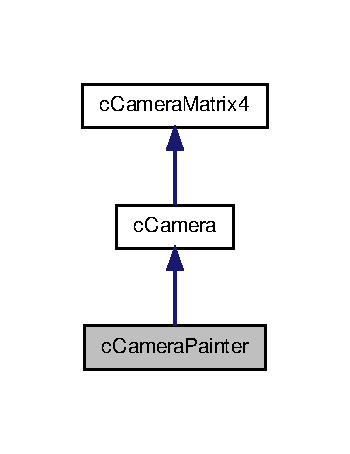
\includegraphics[width=168pt]{classc_camera_painter__inherit__graph}
\end{center}
\end{figure}


Collaboration diagram for cCameraPainter:
\nopagebreak
\begin{figure}[H]
\begin{center}
\leavevmode
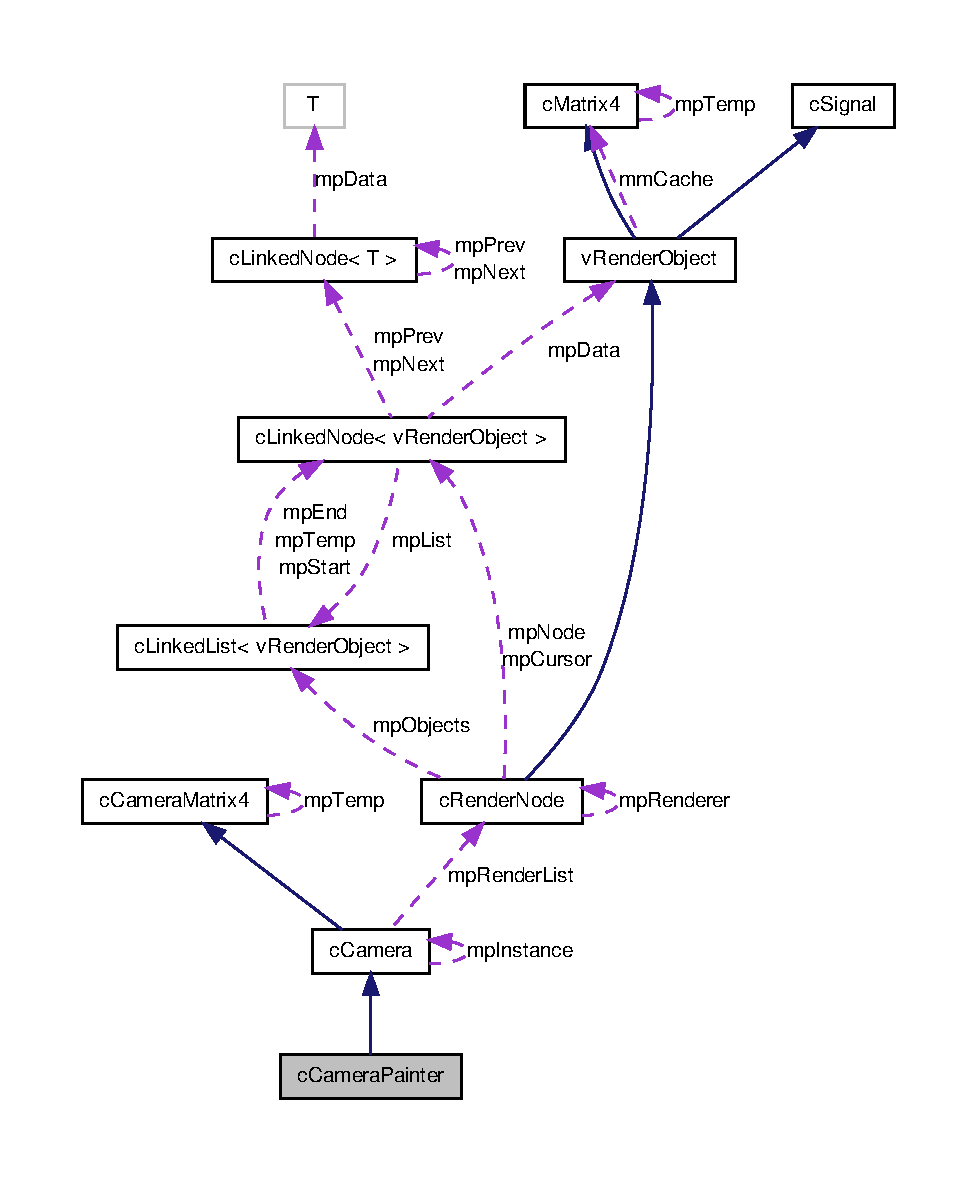
\includegraphics[width=400pt]{classc_camera_painter__coll__graph}
\end{center}
\end{figure}
\subsection*{Public Member Functions}
\begin{DoxyCompactItemize}
\item 
void \hyperlink{classc_camera_painter_abc09c0cb4f02df2cc0b1407f7273a068}{Render} ()
\begin{DoxyCompactList}\small\item\em This function will render the scene graph to \hyperlink{classc_painter}{cPainter} instead of the screen. This is used if WT\_\-USE\_\-PAINTER is set to true. \item\end{DoxyCompactList}\end{DoxyCompactItemize}
\subsection*{Friends}
\begin{DoxyCompactItemize}
\item 
class \hyperlink{classc_camera_painter_a930db2797d94f26b57e430e155ad81ba}{cCamera}
\end{DoxyCompactItemize}


\subsection{Detailed Description}


Definition at line 82 of file WTcCamera.h.



\subsection{Member Function Documentation}
\hypertarget{classc_camera_painter_abc09c0cb4f02df2cc0b1407f7273a068}{
\index{cCameraPainter@{cCameraPainter}!Render@{Render}}
\index{Render@{Render}!cCameraPainter@{cCameraPainter}}
\subsubsection[{Render}]{\setlength{\rightskip}{0pt plus 5cm}void cCameraPainter::Render (
\begin{DoxyParamCaption}
{}
\end{DoxyParamCaption}
)\hspace{0.3cm}{\ttfamily  \mbox{[}virtual\mbox{]}}}}
\label{classc_camera_painter_abc09c0cb4f02df2cc0b1407f7273a068}


This function will render the scene graph to \hyperlink{classc_painter}{cPainter} instead of the screen. This is used if WT\_\-USE\_\-PAINTER is set to true. 



Reimplemented from \hyperlink{classc_camera_acfe96d0953540fa3938e4d415d7cb791}{cCamera}.



Definition at line 47 of file WTcCamera.cpp.



\subsection{Friends And Related Function Documentation}
\hypertarget{classc_camera_painter_a930db2797d94f26b57e430e155ad81ba}{
\index{cCameraPainter@{cCameraPainter}!cCamera@{cCamera}}
\index{cCamera@{cCamera}!cCameraPainter@{cCameraPainter}}
\subsubsection[{cCamera}]{\setlength{\rightskip}{0pt plus 5cm}friend class {\bf cCamera}\hspace{0.3cm}{\ttfamily  \mbox{[}friend\mbox{]}}}}
\label{classc_camera_painter_a930db2797d94f26b57e430e155ad81ba}


Definition at line 88 of file WTcCamera.h.


\hypertarget{classc_cluster}{
\section{cCluster Class Reference}
\label{classc_cluster}\index{cCluster@{cCluster}}
}


This class is an array of \hyperlink{classc_face}{cFace}. This is often used.  




Collaboration diagram for cCluster:\nopagebreak
\begin{figure}[H]
\begin{center}
\leavevmode
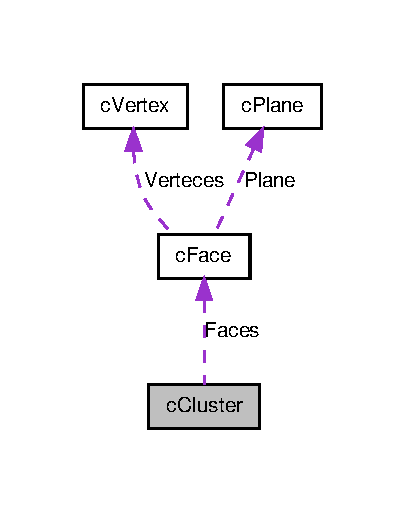
\includegraphics[width=134pt]{classc_cluster__coll__graph}
\end{center}
\end{figure}


\subsection{Detailed Description}
This class is an array of \hyperlink{classc_face}{cFace}. This is often used. 
\hypertarget{classc_cluster_list}{
\section{cClusterList Class Reference}
\label{classc_cluster_list}\index{cClusterList@{cClusterList}}
}


Inheritance diagram for cClusterList:
\nopagebreak
\begin{figure}[H]
\begin{center}
\leavevmode
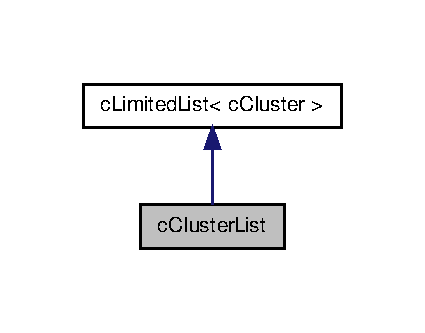
\includegraphics[width=204pt]{classc_cluster_list__inherit__graph}
\end{center}
\end{figure}


Collaboration diagram for cClusterList:
\nopagebreak
\begin{figure}[H]
\begin{center}
\leavevmode
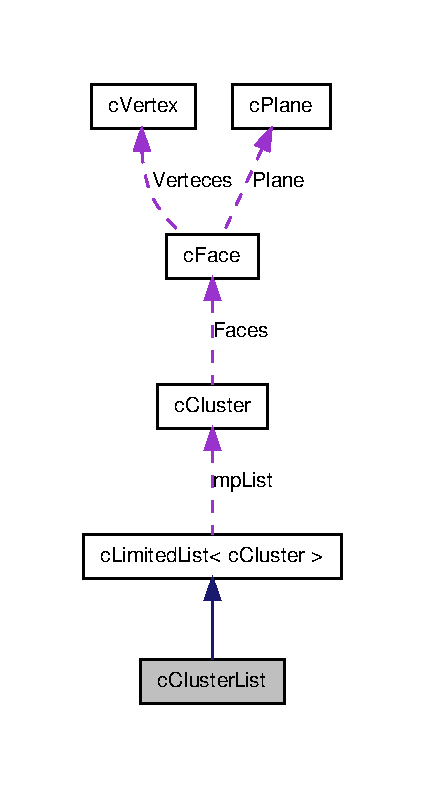
\includegraphics[width=204pt]{classc_cluster_list__coll__graph}
\end{center}
\end{figure}
\subsection*{Public Member Functions}
\begin{DoxyCompactItemize}
\item 
\hyperlink{classc_cluster_list_ae909636c143cd82ff5c225ddec08f395}{cClusterList} ()
\item 
\hyperlink{classc_cluster_list_a66f2d8682c3b5560aad47b8619771007}{$\sim$cClusterList} ()
\item 
void \hyperlink{classc_cluster_list_a4cfd14c5029479723ae1adb36a22696c}{Optimise} ()
\item 
void \hyperlink{classc_cluster_list_a38f0863da90eb645b157cb3e88d3cd9a}{GenerateClusters} (\hyperlink{classc_full_face_list}{cFullFaceList} \&ClusterData)
\item 
void \hyperlink{classc_cluster_list_add154dae70923fdf275dbffbe2535bc6}{GenerateConvex} (\hyperlink{classc_full_face_list}{cFullFaceList} \&ClusterData)
\item 
void \hyperlink{classc_cluster_list_a09dfd33c463dce1fbb7a29ff27ffe862}{GenerateConcaves} (\hyperlink{classc_full_face_list}{cFullFaceList} \&ClusterData)
\item 
void \hyperlink{classc_cluster_list_a9f8d98763d7af125635aaa2488afee3b}{OutputIMFClusters} (ofstream \&FileStream)
\item 
void \hyperlink{classc_cluster_list_a3ac8e6f8754c8689d04daee9c1585c05}{LoadIMFClusters} (ifstream \&FileStream)
\item 
uint32 \hyperlink{classc_cluster_list_ad2c3108ecb26ad68438f9e2ab14c0775}{FileSize} ()
\end{DoxyCompactItemize}


\subsection{Detailed Description}


Definition at line 36 of file WTcCluster.h.



\subsection{Constructor \& Destructor Documentation}
\hypertarget{classc_cluster_list_ae909636c143cd82ff5c225ddec08f395}{
\index{cClusterList@{cClusterList}!cClusterList@{cClusterList}}
\index{cClusterList@{cClusterList}!cClusterList@{cClusterList}}
\subsubsection[{cClusterList}]{\setlength{\rightskip}{0pt plus 5cm}cClusterList::cClusterList (
\begin{DoxyParamCaption}
{}
\end{DoxyParamCaption}
)\hspace{0.3cm}{\ttfamily  \mbox{[}inline\mbox{]}}}}
\label{classc_cluster_list_ae909636c143cd82ff5c225ddec08f395}


Definition at line 40 of file WTcCluster.h.

\hypertarget{classc_cluster_list_a66f2d8682c3b5560aad47b8619771007}{
\index{cClusterList@{cClusterList}!$\sim$cClusterList@{$\sim$cClusterList}}
\index{$\sim$cClusterList@{$\sim$cClusterList}!cClusterList@{cClusterList}}
\subsubsection[{$\sim$cClusterList}]{\setlength{\rightskip}{0pt plus 5cm}cClusterList::$\sim$cClusterList (
\begin{DoxyParamCaption}
{}
\end{DoxyParamCaption}
)\hspace{0.3cm}{\ttfamily  \mbox{[}inline\mbox{]}}}}
\label{classc_cluster_list_a66f2d8682c3b5560aad47b8619771007}


Definition at line 41 of file WTcCluster.h.



\subsection{Member Function Documentation}
\hypertarget{classc_cluster_list_ad2c3108ecb26ad68438f9e2ab14c0775}{
\index{cClusterList@{cClusterList}!FileSize@{FileSize}}
\index{FileSize@{FileSize}!cClusterList@{cClusterList}}
\subsubsection[{FileSize}]{\setlength{\rightskip}{0pt plus 5cm}uint32 cClusterList::FileSize (
\begin{DoxyParamCaption}
{}
\end{DoxyParamCaption}
)\hspace{0.3cm}{\ttfamily  \mbox{[}inline\mbox{]}}}}
\label{classc_cluster_list_ad2c3108ecb26ad68438f9e2ab14c0775}


Definition at line 68 of file WTcCluster.h.

\hypertarget{classc_cluster_list_a38f0863da90eb645b157cb3e88d3cd9a}{
\index{cClusterList@{cClusterList}!GenerateClusters@{GenerateClusters}}
\index{GenerateClusters@{GenerateClusters}!cClusterList@{cClusterList}}
\subsubsection[{GenerateClusters}]{\setlength{\rightskip}{0pt plus 5cm}void cClusterList::GenerateClusters (
\begin{DoxyParamCaption}
\item[{{\bf cFullFaceList} \&}]{ClusterData}
\end{DoxyParamCaption}
)}}
\label{classc_cluster_list_a38f0863da90eb645b157cb3e88d3cd9a}


Definition at line 80 of file WTcCluster.cpp.

\hypertarget{classc_cluster_list_a09dfd33c463dce1fbb7a29ff27ffe862}{
\index{cClusterList@{cClusterList}!GenerateConcaves@{GenerateConcaves}}
\index{GenerateConcaves@{GenerateConcaves}!cClusterList@{cClusterList}}
\subsubsection[{GenerateConcaves}]{\setlength{\rightskip}{0pt plus 5cm}void cClusterList::GenerateConcaves (
\begin{DoxyParamCaption}
\item[{{\bf cFullFaceList} \&}]{ClusterData}
\end{DoxyParamCaption}
)}}
\label{classc_cluster_list_a09dfd33c463dce1fbb7a29ff27ffe862}


Definition at line 48 of file WTcCluster.cpp.

\hypertarget{classc_cluster_list_add154dae70923fdf275dbffbe2535bc6}{
\index{cClusterList@{cClusterList}!GenerateConvex@{GenerateConvex}}
\index{GenerateConvex@{GenerateConvex}!cClusterList@{cClusterList}}
\subsubsection[{GenerateConvex}]{\setlength{\rightskip}{0pt plus 5cm}void cClusterList::GenerateConvex (
\begin{DoxyParamCaption}
\item[{{\bf cFullFaceList} \&}]{ClusterData}
\end{DoxyParamCaption}
)}}
\label{classc_cluster_list_add154dae70923fdf275dbffbe2535bc6}


Definition at line 24 of file WTcCluster.cpp.

\hypertarget{classc_cluster_list_a3ac8e6f8754c8689d04daee9c1585c05}{
\index{cClusterList@{cClusterList}!LoadIMFClusters@{LoadIMFClusters}}
\index{LoadIMFClusters@{LoadIMFClusters}!cClusterList@{cClusterList}}
\subsubsection[{LoadIMFClusters}]{\setlength{\rightskip}{0pt plus 5cm}void cClusterList::LoadIMFClusters (
\begin{DoxyParamCaption}
\item[{ifstream \&}]{FileStream}
\end{DoxyParamCaption}
)\hspace{0.3cm}{\ttfamily  \mbox{[}inline\mbox{]}}}}
\label{classc_cluster_list_a3ac8e6f8754c8689d04daee9c1585c05}


Definition at line 57 of file WTcCluster.h.

\hypertarget{classc_cluster_list_a4cfd14c5029479723ae1adb36a22696c}{
\index{cClusterList@{cClusterList}!Optimise@{Optimise}}
\index{Optimise@{Optimise}!cClusterList@{cClusterList}}
\subsubsection[{Optimise}]{\setlength{\rightskip}{0pt plus 5cm}void cClusterList::Optimise (
\begin{DoxyParamCaption}
{}
\end{DoxyParamCaption}
)}}
\label{classc_cluster_list_a4cfd14c5029479723ae1adb36a22696c}


Definition at line 9 of file WTcCluster.cpp.

\hypertarget{classc_cluster_list_a9f8d98763d7af125635aaa2488afee3b}{
\index{cClusterList@{cClusterList}!OutputIMFClusters@{OutputIMFClusters}}
\index{OutputIMFClusters@{OutputIMFClusters}!cClusterList@{cClusterList}}
\subsubsection[{OutputIMFClusters}]{\setlength{\rightskip}{0pt plus 5cm}void cClusterList::OutputIMFClusters (
\begin{DoxyParamCaption}
\item[{ofstream \&}]{FileStream}
\end{DoxyParamCaption}
)\hspace{0.3cm}{\ttfamily  \mbox{[}inline\mbox{]}}}}
\label{classc_cluster_list_a9f8d98763d7af125635aaa2488afee3b}


Definition at line 47 of file WTcCluster.h.


\hypertarget{classc_collision_handler}{
\section{cCollisionHandler Class Reference}
\label{classc_collision_handler}\index{cCollisionHandler@{cCollisionHandler}}
}


This is the Collision Handler. It will control any collision search the user performs. This Collision handler is created by using the \hyperlink{classc_collision_handler_a04d5c8d5b7ac854b4958dca195bf1c1b}{Instance()} and can ONLY be created using \hyperlink{classc_collision_handler_a04d5c8d5b7ac854b4958dca195bf1c1b}{Instance()}. \_\-COLLISION\_\-HANDLER is a quick pointer to the \hyperlink{classc_collision_handler_a04d5c8d5b7ac854b4958dca195bf1c1b}{cCollisionHandler::Instance()} pointer. This will store data for the search and will store the current position to resume searches. Calling the Function GenerateCollisionList() wil create a comprehensive list of pointers to cRenderobjects() that meet the collision parameters of GenerateCollisionList(). This list can be accessed by using NextCollisionItem().  




Collaboration diagram for cCollisionHandler:\nopagebreak
\begin{figure}[H]
\begin{center}
\leavevmode
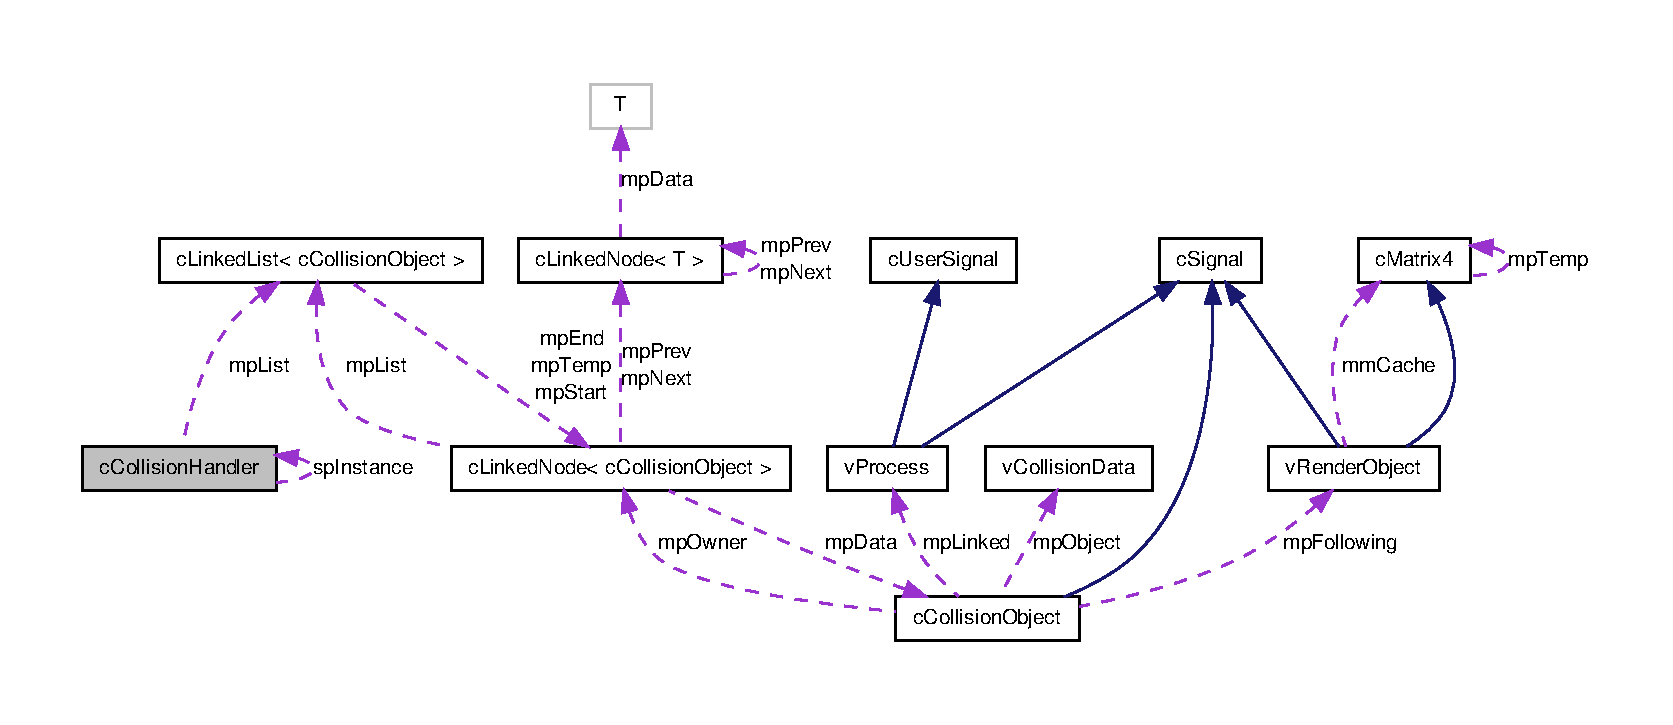
\includegraphics[width=400pt]{classc_collision_handler__coll__graph}
\end{center}
\end{figure}
\subsection*{Public Member Functions}
\begin{DoxyCompactItemize}
\item 
\hypertarget{classc_collision_handler_a5810098e3ca35eac5cb23936840787ef}{
virtual \hyperlink{classc_collision_handler_a5810098e3ca35eac5cb23936840787ef}{$\sim$cCollisionHandler} ()}
\label{classc_collision_handler_a5810098e3ca35eac5cb23936840787ef}

\begin{DoxyCompactList}\small\item\em This will deconstruct the class. \end{DoxyCompactList}\item 
\hypertarget{classc_collision_handler_a4fe00bffd2defe0a71a17c5fadd3b890}{
virtual void \hyperlink{classc_collision_handler_a4fe00bffd2defe0a71a17c5fadd3b890}{ResetCursors} ()=0}
\label{classc_collision_handler_a4fe00bffd2defe0a71a17c5fadd3b890}

\begin{DoxyCompactList}\small\item\em This will reset both the cursors used to track position through the collision object lists. \end{DoxyCompactList}\end{DoxyCompactItemize}
\subsection*{Static Public Member Functions}
\begin{DoxyCompactItemize}
\item 
\hypertarget{classc_collision_handler_a04d5c8d5b7ac854b4958dca195bf1c1b}{
static \hyperlink{classc_collision_handler}{cCollisionHandler} $\ast$ \hyperlink{classc_collision_handler_a04d5c8d5b7ac854b4958dca195bf1c1b}{Instance} ()}
\label{classc_collision_handler_a04d5c8d5b7ac854b4958dca195bf1c1b}

\begin{DoxyCompactList}\small\item\em This will return a pointer to the classes current instance and if there is none it will create one. \end{DoxyCompactList}\end{DoxyCompactItemize}
\subsection*{Protected Member Functions}
\begin{DoxyCompactItemize}
\item 
\hypertarget{classc_collision_handler_ae966359105ed5e144f62e36dd85d1f03}{
virtual \hyperlink{classc_linked_node}{cLinkedNode}$<$ \hyperlink{classc_collision_object}{cCollisionObject} $>$ $\ast$ \hyperlink{classc_collision_handler_ae966359105ed5e144f62e36dd85d1f03}{Add} (\hyperlink{classc_collision_object}{cCollisionObject} $\ast$lpTemp)=0}
\label{classc_collision_handler_ae966359105ed5e144f62e36dd85d1f03}

\begin{DoxyCompactList}\small\item\em This will add the \hyperlink{classc_collision_object}{cCollisionObject} pointed to by lpObject to the list mpList. \end{DoxyCompactList}\item 
\hypertarget{classc_collision_handler_aec2e30bb6be227d30daef0b6eb36d3b3}{
virtual void \hyperlink{classc_collision_handler_aec2e30bb6be227d30daef0b6eb36d3b3}{Remove} (\hyperlink{classc_linked_node}{cLinkedNode}$<$ \hyperlink{classc_collision_object}{cCollisionObject} $>$ $\ast$lpOld)}
\label{classc_collision_handler_aec2e30bb6be227d30daef0b6eb36d3b3}

\begin{DoxyCompactList}\small\item\em This will turn off Collisions for the \hyperlink{classc_linked_node}{cLinkedNode} lpOld. This should in turn call \hyperlink{classc_collision_handler_ad2d0933b78c692a5d2b3885242fa0911}{RemoveFromList()}. \end{DoxyCompactList}\item 
\hypertarget{classc_collision_handler_ad2d0933b78c692a5d2b3885242fa0911}{
virtual void \hyperlink{classc_collision_handler_ad2d0933b78c692a5d2b3885242fa0911}{RemoveFromList} (\hyperlink{classc_linked_node}{cLinkedNode}$<$ \hyperlink{classc_collision_object}{cCollisionObject} $>$ $\ast$lpOld)}
\label{classc_collision_handler_ad2d0933b78c692a5d2b3885242fa0911}

\begin{DoxyCompactList}\small\item\em This will acutally remove the clinkedNode from the relevant list. \end{DoxyCompactList}\item 
\hypertarget{classc_collision_handler_a906305fe520cefc195f3948458aba941}{
virtual bool \hyperlink{classc_collision_handler_a906305fe520cefc195f3948458aba941}{NextListItem} ()}
\label{classc_collision_handler_a906305fe520cefc195f3948458aba941}

\begin{DoxyCompactList}\small\item\em This will return the Next item in the lists in order. (The item is pointed to by mpColCur). If an item is found will return true, else will return false. \end{DoxyCompactList}\item 
\hypertarget{classc_collision_handler_a58b636db8343b7f4bbb27f3a93799e8b}{
virtual bool \hyperlink{classc_collision_handler_a58b636db8343b7f4bbb27f3a93799e8b}{NextListItem} (uint32 lpType)}
\label{classc_collision_handler_a58b636db8343b7f4bbb27f3a93799e8b}

\begin{DoxyCompactList}\small\item\em This will return the Next item in the list storing lpType in order. (the item is pointed to by mpColCur).If an item is found will return true, else will return false. \end{DoxyCompactList}\item 
\hypertarget{classc_collision_handler_ad2b079e234f956301fe83f5a5938cad0}{
virtual uint32 \hyperlink{classc_collision_handler_ad2b079e234f956301fe83f5a5938cad0}{FindSlot} (\hyperlink{classc_collision_object}{cCollisionObject} $\ast$lpObj)}
\label{classc_collision_handler_ad2b079e234f956301fe83f5a5938cad0}

\begin{DoxyCompactList}\small\item\em This will find the appropriate array slot for the \hyperlink{classc_collision_object}{cCollisionObject} lpObj. It will return the array position of the slot. \end{DoxyCompactList}\item 
\hypertarget{classc_collision_handler_aa6f7ca9d10b078ba11fcc3c0d266ab8e}{
virtual \hyperlink{classc_linked_list}{cLinkedList}$<$ \hyperlink{classc_collision_object}{cCollisionObject} $>$ $\ast$ \hyperlink{classc_collision_handler_aa6f7ca9d10b078ba11fcc3c0d266ab8e}{FindSlot} (uint32 $\ast$lpPos)}
\label{classc_collision_handler_aa6f7ca9d10b078ba11fcc3c0d266ab8e}

\begin{DoxyCompactList}\small\item\em This will return the list for the spatial slot lpPos\mbox{[}0\mbox{]},lpPos\mbox{[}1\mbox{]},lpPos\mbox{[}2\mbox{]}. (Array slots not spatial co-\/ordinates). \end{DoxyCompactList}\item 
\hypertarget{classc_collision_handler_aae512b7a5c7abb7307e7d25f22aa9fd0}{
virtual void \hyperlink{classc_collision_handler_aae512b7a5c7abb7307e7d25f22aa9fd0}{Position} (float $\ast$lpTemp)}
\label{classc_collision_handler_aae512b7a5c7abb7307e7d25f22aa9fd0}

\begin{DoxyCompactList}\small\item\em This will set the current Position of the Spatial Array. \end{DoxyCompactList}\item 
\hypertarget{classc_collision_handler_af02385e0c91e4c73c521e65477efed2c}{
virtual float $\ast$ \hyperlink{classc_collision_handler_af02385e0c91e4c73c521e65477efed2c}{Position} ()}
\label{classc_collision_handler_af02385e0c91e4c73c521e65477efed2c}

\begin{DoxyCompactList}\small\item\em This will return the current Position of the Spatial Array. \end{DoxyCompactList}\end{DoxyCompactItemize}
\subsection*{Protected Attributes}
\begin{DoxyCompactItemize}
\item 
\hypertarget{classc_collision_handler_a959870d5beee77a014b29e45bf153723}{
\hyperlink{classc_linked_list}{cLinkedList}$<$ \hyperlink{classc_collision_object}{cCollisionObject} $>$ $\ast$ \hyperlink{classc_collision_handler_a959870d5beee77a014b29e45bf153723}{mpList}}
\label{classc_collision_handler_a959870d5beee77a014b29e45bf153723}

\begin{DoxyCompactList}\small\item\em This is an array for storing all Collision Objects, that are currently on. The size of the array is set by WT\_\-COLLISION\_\-HANDLER\_\-ARRAY\_\-SIZE. \end{DoxyCompactList}\end{DoxyCompactItemize}
\subsection*{Static Protected Attributes}
\begin{DoxyCompactItemize}
\item 
\hypertarget{classc_collision_handler_ae020327c284763548d259a3d35a8f537}{
static \hyperlink{classc_collision_handler}{cCollisionHandler} $\ast$ \hyperlink{classc_collision_handler_ae020327c284763548d259a3d35a8f537}{spInstance}}
\label{classc_collision_handler_ae020327c284763548d259a3d35a8f537}

\begin{DoxyCompactList}\small\item\em This is a pointer to the classes current instance. There can only be one... \end{DoxyCompactList}\end{DoxyCompactItemize}
\subsection*{Friends}
\begin{DoxyCompactItemize}
\item 
\hypertarget{classc_collision_handler_a3fc30c810c62135f498c47205c853e30}{
class \hyperlink{classc_collision_handler_a3fc30c810c62135f498c47205c853e30}{cCollisionObject}}
\label{classc_collision_handler_a3fc30c810c62135f498c47205c853e30}

\end{DoxyCompactItemize}


\subsection{Detailed Description}
This is the Collision Handler. It will control any collision search the user performs. This Collision handler is created by using the \hyperlink{classc_collision_handler_a04d5c8d5b7ac854b4958dca195bf1c1b}{Instance()} and can ONLY be created using \hyperlink{classc_collision_handler_a04d5c8d5b7ac854b4958dca195bf1c1b}{Instance()}. \_\-COLLISION\_\-HANDLER is a quick pointer to the \hyperlink{classc_collision_handler_a04d5c8d5b7ac854b4958dca195bf1c1b}{cCollisionHandler::Instance()} pointer. This will store data for the search and will store the current position to resume searches. Calling the Function GenerateCollisionList() wil create a comprehensive list of pointers to cRenderobjects() that meet the collision parameters of GenerateCollisionList(). This list can be accessed by using NextCollisionItem(). 

The sizes and positions of objects are calculated during a render cycle. ????Objects will not collide until after their first render cycle.

There are three types of Collision Searches. Tree, Type and Binary Spatial Position. (defined by setting WT\_\-COLLISION\_\-HANDLER\_\-TYPE to WT\_\-COLLISION\_\-HANDLER\_\-TYPE\_\-TYPE or WT\_\-COLLISION\_\-HANDLER\_\-TYPE\_\-BSP.

Tree searches are performed by traversing the render tree. Each objects size is based on the size of the objects beneath it so if a Node does not collide all objects beneath that node can be ignored.

Type searches are filtered by type. cCollisionObject's are given a \hyperlink{classc_collision_object_a2a527f445a899adafbf18dddf140e179}{cCollisionObject::CollisionFilter(uint32 liID)} using which they are sorted into seperate lists of Collision objects. If a search is performed with a defined ID term, only the list containing objects with the desired filter value are searched.

Binary Spatial Position Collision Handlers sort cCollisionObjects into the spatial boxes they contact with. This means it is only neccessary to check other objects within the boxes the current object resides within. 
\hypertarget{classc_collision_handler_b_s_p}{
\section{cCollisionHandlerBSP Class Reference}
\label{classc_collision_handler_b_s_p}\index{cCollisionHandlerBSP@{cCollisionHandlerBSP}}
}


Inheritance diagram for cCollisionHandlerBSP:
\nopagebreak
\begin{figure}[H]
\begin{center}
\leavevmode
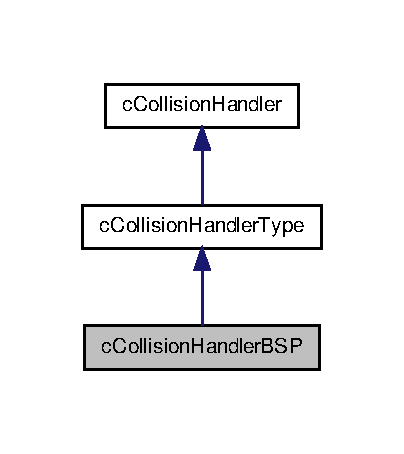
\includegraphics[width=194pt]{classc_collision_handler_b_s_p__inherit__graph}
\end{center}
\end{figure}


Collaboration diagram for cCollisionHandlerBSP:
\nopagebreak
\begin{figure}[H]
\begin{center}
\leavevmode
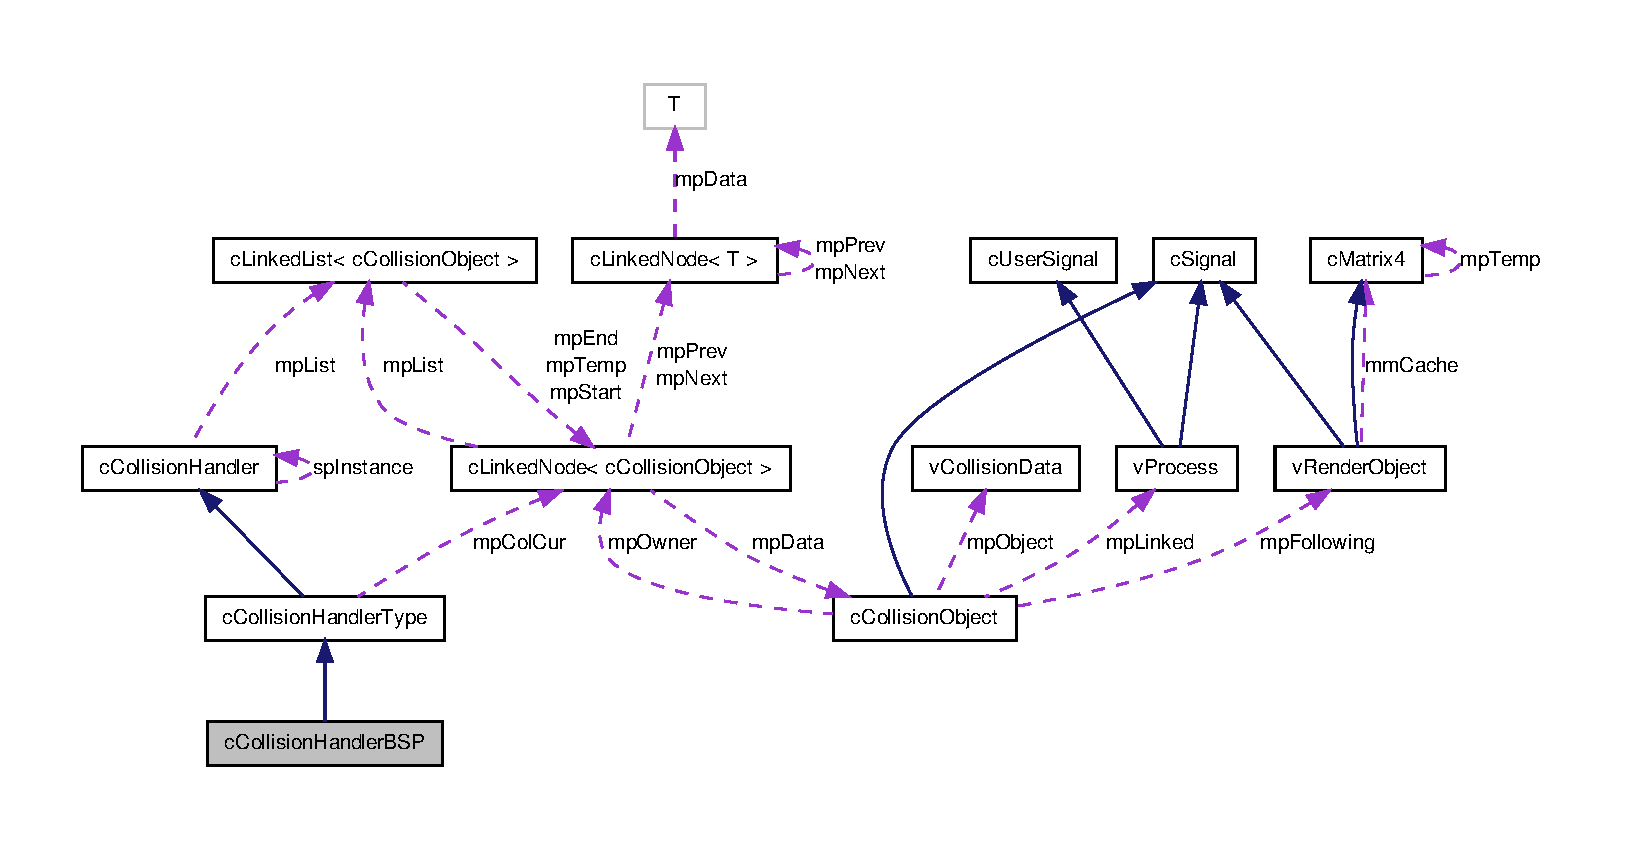
\includegraphics[width=400pt]{classc_collision_handler_b_s_p__coll__graph}
\end{center}
\end{figure}
\subsection*{Public Member Functions}
\begin{DoxyCompactItemize}
\item 
\hyperlink{classc_collision_list}{cCollisionList} $\ast$ \hyperlink{classc_collision_handler_b_s_p_a3eefab2420c94920816fc63932140b5f}{GenerateCollisionList} (\hyperlink{classc_collision_object}{cCollisionObject} $\ast$lpObj, uint32 lpType=0)
\begin{DoxyCompactList}\small\item\em This will Actually search the Collision Lists and create a mpCollisionList with all the detected collisions with objects of type lpType. \item\end{DoxyCompactList}\item 
void \hyperlink{classc_collision_handler_b_s_p_a8fb831211d5d23d6a0ce1e77c1a011bf}{Position} (float $\ast$lpTemp)
\begin{DoxyCompactList}\small\item\em This will set the current Position of the Spatial Array. \item\end{DoxyCompactList}\item 
float $\ast$ \hyperlink{classc_collision_handler_b_s_p_a44158a68c715d0f4cd82e4f281554bfd}{Position} ()
\begin{DoxyCompactList}\small\item\em This will return the current Position of the Spatial Array. \item\end{DoxyCompactList}\item 
uint32 \hyperlink{classc_collision_handler_b_s_p_a9dfe5f431663f6e73fe9bac7f5225b6b}{FindSlot} (\hyperlink{classc_collision_object}{cCollisionObject} $\ast$lpObj)
\begin{DoxyCompactList}\small\item\em This will find the appropriate array slot for the \hyperlink{classc_collision_object}{cCollisionObject} lpObj. It will return the array position of the slot. \item\end{DoxyCompactList}\item 
uint32 \hyperlink{classc_collision_handler_b_s_p_a6aa114aa26cbac205816bf1338e04d82}{FindSlot} (float $\ast$lpPos)
\begin{DoxyCompactList}\small\item\em This will Find the Spatial Slot for the position lpPos. \item\end{DoxyCompactList}\item 
\hyperlink{classc_linked_list}{cLinkedList}$<$ \hyperlink{classc_collision_object}{cCollisionObject} $>$ $\ast$ \hyperlink{classc_collision_handler_b_s_p_a08fa8650b8200a442b68c123220d7c40}{FindSlot} (uint32 $\ast$lpPos)
\begin{DoxyCompactList}\small\item\em This will return the list for the spatial slot lpPos\mbox{[}0\mbox{]},lpPos\mbox{[}1\mbox{]},lpPos\mbox{[}2\mbox{]}. (Array slots not spatial co-\/ordinates). \item\end{DoxyCompactList}\item 
virtual \hyperlink{classc_collision_handler_b_s_p_a44222f6325b435e75bf2325f3b98c629}{$\sim$cCollisionHandlerBSP} ()
\end{DoxyCompactItemize}
\subsection*{Protected Member Functions}
\begin{DoxyCompactItemize}
\item 
\hyperlink{classc_collision_handler_b_s_p_a39c5eaabff78246918df294b1f5492d9}{cCollisionHandlerBSP} ()
\end{DoxyCompactItemize}
\subsection*{Protected Attributes}
\begin{DoxyCompactItemize}
\item 
float \hyperlink{classc_collision_handler_b_s_p_a2f5ddea62a1158ccdfc29539a9c23a8d}{mfCentre} \mbox{[}3\mbox{]}
\begin{DoxyCompactList}\small\item\em This stores the Current central position of the Spatial Array. \item\end{DoxyCompactList}\end{DoxyCompactItemize}
\subsection*{Static Protected Attributes}
\begin{DoxyCompactItemize}
\item 
static uint32 \hyperlink{classc_collision_handler_b_s_p_a521e19fe8bb2a85bda87223955b2f696}{mpAxisOrder} \mbox{[}3\mbox{]} = \{0,2,1\}
\begin{DoxyCompactList}\small\item\em This makes arrays dimensions order in X,Z,Y without hard coding it. (1D is X Axis, 2D is X,Z axis and 3D is X,Z,Y axis). \item\end{DoxyCompactList}\end{DoxyCompactItemize}
\subsection*{Friends}
\begin{DoxyCompactItemize}
\item 
class \hyperlink{classc_collision_handler_b_s_p_a2dee8095fea5c5aa41fe4060393f31ad}{cCollisionHandler}
\end{DoxyCompactItemize}


\subsection{Detailed Description}


Definition at line 143 of file WTcCollisionHandler.h.



\subsection{Constructor \& Destructor Documentation}
\hypertarget{classc_collision_handler_b_s_p_a39c5eaabff78246918df294b1f5492d9}{
\index{cCollisionHandlerBSP@{cCollisionHandlerBSP}!cCollisionHandlerBSP@{cCollisionHandlerBSP}}
\index{cCollisionHandlerBSP@{cCollisionHandlerBSP}!cCollisionHandlerBSP@{cCollisionHandlerBSP}}
\subsubsection[{cCollisionHandlerBSP}]{\setlength{\rightskip}{0pt plus 5cm}cCollisionHandlerBSP::cCollisionHandlerBSP (
\begin{DoxyParamCaption}
{}
\end{DoxyParamCaption}
)\hspace{0.3cm}{\ttfamily  \mbox{[}protected\mbox{]}}}}
\label{classc_collision_handler_b_s_p_a39c5eaabff78246918df294b1f5492d9}


Definition at line 139 of file WTcCollisionHandler.cpp.

\hypertarget{classc_collision_handler_b_s_p_a44222f6325b435e75bf2325f3b98c629}{
\index{cCollisionHandlerBSP@{cCollisionHandlerBSP}!$\sim$cCollisionHandlerBSP@{$\sim$cCollisionHandlerBSP}}
\index{$\sim$cCollisionHandlerBSP@{$\sim$cCollisionHandlerBSP}!cCollisionHandlerBSP@{cCollisionHandlerBSP}}
\subsubsection[{$\sim$cCollisionHandlerBSP}]{\setlength{\rightskip}{0pt plus 5cm}cCollisionHandlerBSP::$\sim$cCollisionHandlerBSP (
\begin{DoxyParamCaption}
{}
\end{DoxyParamCaption}
)\hspace{0.3cm}{\ttfamily  \mbox{[}virtual\mbox{]}}}}
\label{classc_collision_handler_b_s_p_a44222f6325b435e75bf2325f3b98c629}


Definition at line 78 of file WTcCollisionHandler.cpp.



\subsection{Member Function Documentation}
\hypertarget{classc_collision_handler_b_s_p_a9dfe5f431663f6e73fe9bac7f5225b6b}{
\index{cCollisionHandlerBSP@{cCollisionHandlerBSP}!FindSlot@{FindSlot}}
\index{FindSlot@{FindSlot}!cCollisionHandlerBSP@{cCollisionHandlerBSP}}
\subsubsection[{FindSlot}]{\setlength{\rightskip}{0pt plus 5cm}uint32 cCollisionHandlerBSP::FindSlot (
\begin{DoxyParamCaption}
\item[{{\bf cCollisionObject} $\ast$}]{lpObj}
\end{DoxyParamCaption}
)\hspace{0.3cm}{\ttfamily  \mbox{[}virtual\mbox{]}}}}
\label{classc_collision_handler_b_s_p_a9dfe5f431663f6e73fe9bac7f5225b6b}


This will find the appropriate array slot for the \hyperlink{classc_collision_object}{cCollisionObject} lpObj. It will return the array position of the slot. 



Reimplemented from \hyperlink{classc_collision_handler_type_a6935d209eccb9c605fac6208c61b98b7}{cCollisionHandlerType}.



Definition at line 190 of file WTcCollisionHandler.cpp.

\hypertarget{classc_collision_handler_b_s_p_a6aa114aa26cbac205816bf1338e04d82}{
\index{cCollisionHandlerBSP@{cCollisionHandlerBSP}!FindSlot@{FindSlot}}
\index{FindSlot@{FindSlot}!cCollisionHandlerBSP@{cCollisionHandlerBSP}}
\subsubsection[{FindSlot}]{\setlength{\rightskip}{0pt plus 5cm}uint32 cCollisionHandlerBSP::FindSlot (
\begin{DoxyParamCaption}
\item[{float $\ast$}]{lpPos}
\end{DoxyParamCaption}
)\hspace{0.3cm}{\ttfamily  \mbox{[}virtual\mbox{]}}}}
\label{classc_collision_handler_b_s_p_a6aa114aa26cbac205816bf1338e04d82}


This will Find the Spatial Slot for the position lpPos. 



Reimplemented from \hyperlink{classc_collision_handler_type_aef03e4dfc78ee53e0ebee35456412352}{cCollisionHandlerType}.



Definition at line 161 of file WTcCollisionHandler.cpp.

\hypertarget{classc_collision_handler_b_s_p_a08fa8650b8200a442b68c123220d7c40}{
\index{cCollisionHandlerBSP@{cCollisionHandlerBSP}!FindSlot@{FindSlot}}
\index{FindSlot@{FindSlot}!cCollisionHandlerBSP@{cCollisionHandlerBSP}}
\subsubsection[{FindSlot}]{\setlength{\rightskip}{0pt plus 5cm}{\bf cLinkedList}$<$ {\bf cCollisionObject} $>$ $\ast$ cCollisionHandlerBSP::FindSlot (
\begin{DoxyParamCaption}
\item[{uint32 $\ast$}]{lpPos}
\end{DoxyParamCaption}
)\hspace{0.3cm}{\ttfamily  \mbox{[}virtual\mbox{]}}}}
\label{classc_collision_handler_b_s_p_a08fa8650b8200a442b68c123220d7c40}


This will return the list for the spatial slot lpPos\mbox{[}0\mbox{]},lpPos\mbox{[}1\mbox{]},lpPos\mbox{[}2\mbox{]}. (Array slots not spatial co-\/ordinates). 



Reimplemented from \hyperlink{classc_collision_handler_type_ab9b89db564fb5a2b4881499012443a72}{cCollisionHandlerType}.



Definition at line 197 of file WTcCollisionHandler.cpp.

\hypertarget{classc_collision_handler_b_s_p_a3eefab2420c94920816fc63932140b5f}{
\index{cCollisionHandlerBSP@{cCollisionHandlerBSP}!GenerateCollisionList@{GenerateCollisionList}}
\index{GenerateCollisionList@{GenerateCollisionList}!cCollisionHandlerBSP@{cCollisionHandlerBSP}}
\subsubsection[{GenerateCollisionList}]{\setlength{\rightskip}{0pt plus 5cm}{\bf cCollisionList} $\ast$ cCollisionHandlerBSP::GenerateCollisionList (
\begin{DoxyParamCaption}
\item[{{\bf cCollisionObject} $\ast$}]{lpObj, }
\item[{uint32}]{lpType = {\ttfamily 0}}
\end{DoxyParamCaption}
)\hspace{0.3cm}{\ttfamily  \mbox{[}virtual\mbox{]}}}}
\label{classc_collision_handler_b_s_p_a3eefab2420c94920816fc63932140b5f}


This will Actually search the Collision Lists and create a mpCollisionList with all the detected collisions with objects of type lpType. 



Reimplemented from \hyperlink{classc_collision_handler_type_aaab07676063aa5b0773a1c908b202d53}{cCollisionHandlerType}.



Definition at line 20 of file WTcCollisionHandler.cpp.

\hypertarget{classc_collision_handler_b_s_p_a44158a68c715d0f4cd82e4f281554bfd}{
\index{cCollisionHandlerBSP@{cCollisionHandlerBSP}!Position@{Position}}
\index{Position@{Position}!cCollisionHandlerBSP@{cCollisionHandlerBSP}}
\subsubsection[{Position}]{\setlength{\rightskip}{0pt plus 5cm}float$\ast$ cCollisionHandlerBSP::Position (
\begin{DoxyParamCaption}
{}
\end{DoxyParamCaption}
)\hspace{0.3cm}{\ttfamily  \mbox{[}inline, virtual\mbox{]}}}}
\label{classc_collision_handler_b_s_p_a44158a68c715d0f4cd82e4f281554bfd}


This will return the current Position of the Spatial Array. 



Reimplemented from \hyperlink{classc_collision_handler_type_a708db7524f542b2e1164fc4e7e8ab3dd}{cCollisionHandlerType}.



Definition at line 159 of file WTcCollisionHandler.h.

\hypertarget{classc_collision_handler_b_s_p_a8fb831211d5d23d6a0ce1e77c1a011bf}{
\index{cCollisionHandlerBSP@{cCollisionHandlerBSP}!Position@{Position}}
\index{Position@{Position}!cCollisionHandlerBSP@{cCollisionHandlerBSP}}
\subsubsection[{Position}]{\setlength{\rightskip}{0pt plus 5cm}void cCollisionHandlerBSP::Position (
\begin{DoxyParamCaption}
\item[{float $\ast$}]{lpTemp}
\end{DoxyParamCaption}
)\hspace{0.3cm}{\ttfamily  \mbox{[}inline, virtual\mbox{]}}}}
\label{classc_collision_handler_b_s_p_a8fb831211d5d23d6a0ce1e77c1a011bf}


This will set the current Position of the Spatial Array. 



Reimplemented from \hyperlink{classc_collision_handler_type_a56be05fb67ba225b671c6b38e05cc762}{cCollisionHandlerType}.



Definition at line 157 of file WTcCollisionHandler.h.



\subsection{Friends And Related Function Documentation}
\hypertarget{classc_collision_handler_b_s_p_a2dee8095fea5c5aa41fe4060393f31ad}{
\index{cCollisionHandlerBSP@{cCollisionHandlerBSP}!cCollisionHandler@{cCollisionHandler}}
\index{cCollisionHandler@{cCollisionHandler}!cCollisionHandlerBSP@{cCollisionHandlerBSP}}
\subsubsection[{cCollisionHandler}]{\setlength{\rightskip}{0pt plus 5cm}friend class {\bf cCollisionHandler}\hspace{0.3cm}{\ttfamily  \mbox{[}friend\mbox{]}}}}
\label{classc_collision_handler_b_s_p_a2dee8095fea5c5aa41fe4060393f31ad}


Reimplemented from \hyperlink{classc_collision_handler_type_a2dee8095fea5c5aa41fe4060393f31ad}{cCollisionHandlerType}.



Definition at line 169 of file WTcCollisionHandler.h.



\subsection{Member Data Documentation}
\hypertarget{classc_collision_handler_b_s_p_a2f5ddea62a1158ccdfc29539a9c23a8d}{
\index{cCollisionHandlerBSP@{cCollisionHandlerBSP}!mfCentre@{mfCentre}}
\index{mfCentre@{mfCentre}!cCollisionHandlerBSP@{cCollisionHandlerBSP}}
\subsubsection[{mfCentre}]{\setlength{\rightskip}{0pt plus 5cm}float {\bf cCollisionHandlerBSP::mfCentre}\mbox{[}3\mbox{]}\hspace{0.3cm}{\ttfamily  \mbox{[}protected\mbox{]}}}}
\label{classc_collision_handler_b_s_p_a2f5ddea62a1158ccdfc29539a9c23a8d}


This stores the Current central position of the Spatial Array. 



Definition at line 148 of file WTcCollisionHandler.h.

\hypertarget{classc_collision_handler_b_s_p_a521e19fe8bb2a85bda87223955b2f696}{
\index{cCollisionHandlerBSP@{cCollisionHandlerBSP}!mpAxisOrder@{mpAxisOrder}}
\index{mpAxisOrder@{mpAxisOrder}!cCollisionHandlerBSP@{cCollisionHandlerBSP}}
\subsubsection[{mpAxisOrder}]{\setlength{\rightskip}{0pt plus 5cm}uint32 {\bf cCollisionHandlerBSP::mpAxisOrder} = \{0,2,1\}\hspace{0.3cm}{\ttfamily  \mbox{[}static, protected\mbox{]}}}}
\label{classc_collision_handler_b_s_p_a521e19fe8bb2a85bda87223955b2f696}


This makes arrays dimensions order in X,Z,Y without hard coding it. (1D is X Axis, 2D is X,Z axis and 3D is X,Z,Y axis). 



Definition at line 150 of file WTcCollisionHandler.h.


\hypertarget{classc_collision_handler_type}{
\section{cCollisionHandlerType Class Reference}
\label{classc_collision_handler_type}\index{cCollisionHandlerType@{cCollisionHandlerType}}
}


Inheritance diagram for cCollisionHandlerType:
\nopagebreak
\begin{figure}[H]
\begin{center}
\leavevmode
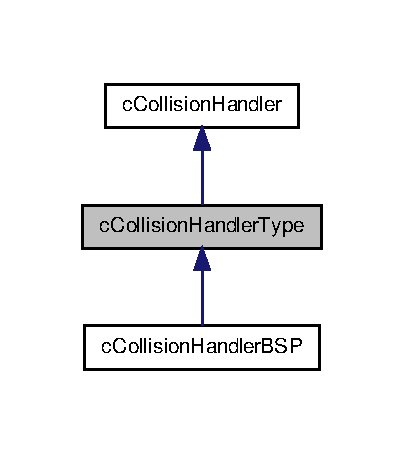
\includegraphics[width=194pt]{classc_collision_handler_type__inherit__graph}
\end{center}
\end{figure}


Collaboration diagram for cCollisionHandlerType:
\nopagebreak
\begin{figure}[H]
\begin{center}
\leavevmode
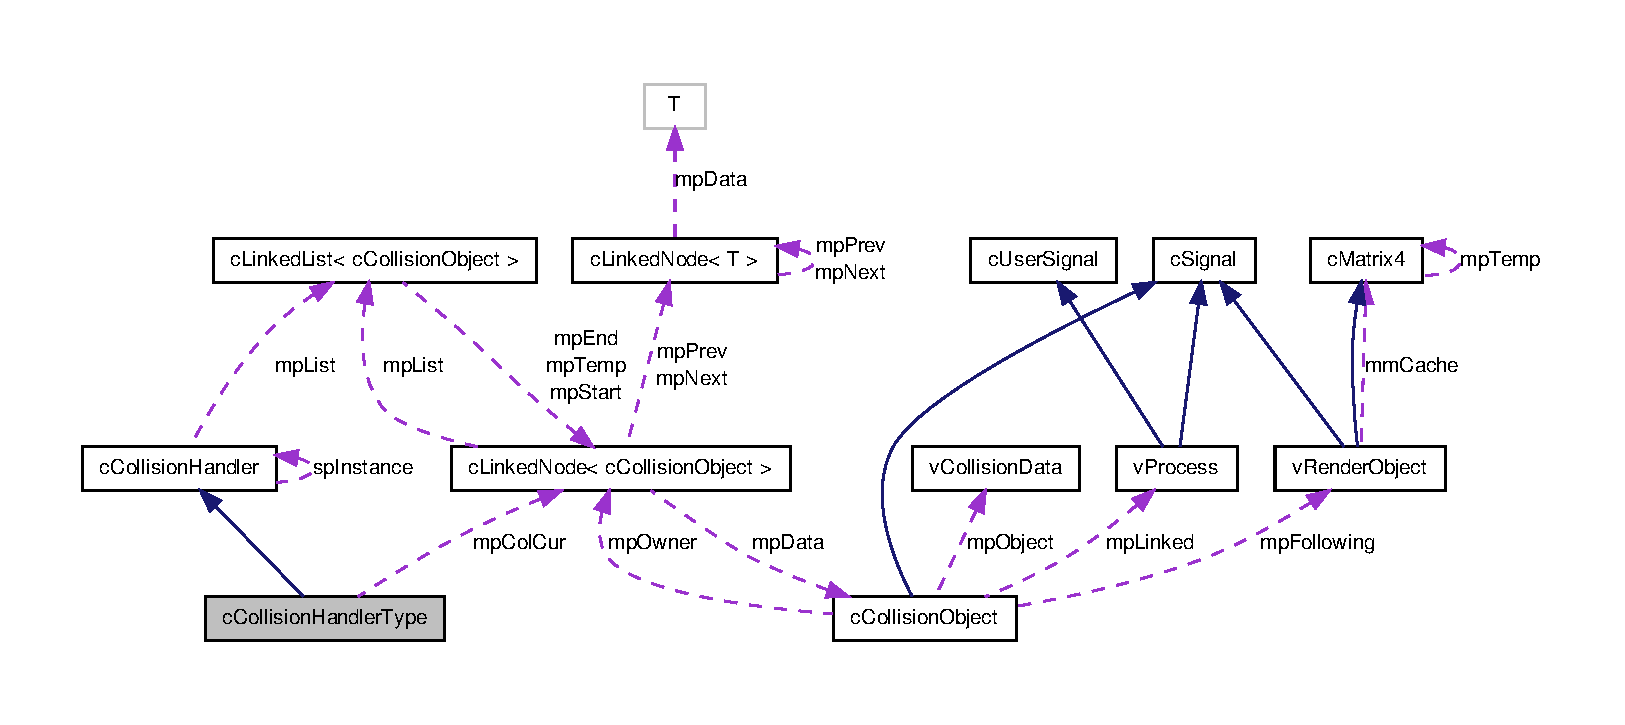
\includegraphics[width=400pt]{classc_collision_handler_type__coll__graph}
\end{center}
\end{figure}
\subsection*{Public Member Functions}
\begin{DoxyCompactItemize}
\item 
virtual \hyperlink{classc_collision_list}{cCollisionList} $\ast$ \hyperlink{classc_collision_handler_type_aaab07676063aa5b0773a1c908b202d53}{GenerateCollisionList} (\hyperlink{classc_collision_object}{cCollisionObject} $\ast$lpObj, uint32 lpType=0)
\begin{DoxyCompactList}\small\item\em This will Actually search the Collision Lists and create a mpCollisionList with all the detected collisions with objects of type lpType. \item\end{DoxyCompactList}\item 
void \hyperlink{classc_collision_handler_type_a3d3300c41d38fa8a14c08dd0b94b6c41}{ResetCursors} ()
\begin{DoxyCompactList}\small\item\em This will reset both the cursors used to track position through the collision object lists. \item\end{DoxyCompactList}\item 
virtual \hyperlink{classc_collision_handler_type_a7da274bc57e20b2c93da79934072d26d}{$\sim$cCollisionHandlerType} ()
\begin{DoxyCompactList}\small\item\em This will deconstruct the class. \item\end{DoxyCompactList}\end{DoxyCompactItemize}
\subsection*{Protected Member Functions}
\begin{DoxyCompactItemize}
\item 
\hyperlink{classc_collision_handler_type_a90fce7fe5fee0c544b0d19f9077fc402}{cCollisionHandlerType} ()
\begin{DoxyCompactList}\small\item\em Private Constructor. \item\end{DoxyCompactList}\item 
\hyperlink{classc_linked_node}{cLinkedNode}$<$ \hyperlink{classc_collision_object}{cCollisionObject} $>$ $\ast$ \hyperlink{classc_collision_handler_type_ae2229ae307688f4a8f6ea7d41621e1e6}{Add} (\hyperlink{classc_collision_object}{cCollisionObject} $\ast$lpTemp)
\begin{DoxyCompactList}\small\item\em This will add the \hyperlink{classc_collision_object}{cCollisionObject} pointed to by lpObject to the list mpList. \item\end{DoxyCompactList}\item 
void \hyperlink{classc_collision_handler_type_a7c1606ae3858a38d90e8db5e4080adda}{Remove} (\hyperlink{classc_linked_node}{cLinkedNode}$<$ \hyperlink{classc_collision_object}{cCollisionObject} $>$ $\ast$lpOld)
\begin{DoxyCompactList}\small\item\em This will turn off Collisions for the \hyperlink{classc_linked_node}{cLinkedNode} lpOld. This should in turn call \hyperlink{classc_collision_handler_type_ae1fae66c56488c1a7920d2394e127f2e}{RemoveFromList()}. \item\end{DoxyCompactList}\item 
void \hyperlink{classc_collision_handler_type_ae1fae66c56488c1a7920d2394e127f2e}{RemoveFromList} (\hyperlink{classc_linked_node}{cLinkedNode}$<$ \hyperlink{classc_collision_object}{cCollisionObject} $>$ $\ast$lpOld)
\begin{DoxyCompactList}\small\item\em This will acutally remove the clinkedNode from the relevant list. \item\end{DoxyCompactList}\item 
bool \hyperlink{classc_collision_handler_type_ace66f4067d9117ce379eb84d3afd2fa7}{NextListItem} ()
\begin{DoxyCompactList}\small\item\em This will return the Next item in the lists in order. (The item is pointed to by mpColCur). If an item is found will return true, else will return false. \item\end{DoxyCompactList}\item 
bool \hyperlink{classc_collision_handler_type_adcf86464b4fd085e86f2c3365f7d3452}{NextListItem} (uint32 lpType)
\begin{DoxyCompactList}\small\item\em This will return the Next item in the list storing lpType in order. (the item is pointed to by mpColCur).If an item is found will return true, else will return false. \item\end{DoxyCompactList}\item 
virtual uint32 \hyperlink{classc_collision_handler_type_a6935d209eccb9c605fac6208c61b98b7}{FindSlot} (\hyperlink{classc_collision_object}{cCollisionObject} $\ast$lpObj)
\begin{DoxyCompactList}\small\item\em This will find the appropriate array slot for the \hyperlink{classc_collision_object}{cCollisionObject} lpObj. It will return the array position of the slot. \item\end{DoxyCompactList}\item 
virtual void \hyperlink{classc_collision_handler_type_a56be05fb67ba225b671c6b38e05cc762}{Position} (float $\ast$lpTemp)
\begin{DoxyCompactList}\small\item\em This will set the current Position of the Spatial Array. \item\end{DoxyCompactList}\item 
virtual float $\ast$ \hyperlink{classc_collision_handler_type_a708db7524f542b2e1164fc4e7e8ab3dd}{Position} ()
\begin{DoxyCompactList}\small\item\em This will return the current Position of the Spatial Array. \item\end{DoxyCompactList}\item 
virtual uint32 \hyperlink{classc_collision_handler_type_aef03e4dfc78ee53e0ebee35456412352}{FindSlot} (float $\ast$lpPos)
\begin{DoxyCompactList}\small\item\em This will Find the Spatial Slot for the position lpPos. \item\end{DoxyCompactList}\item 
virtual \hyperlink{classc_linked_list}{cLinkedList}$<$ \hyperlink{classc_collision_object}{cCollisionObject} $>$ $\ast$ \hyperlink{classc_collision_handler_type_ab9b89db564fb5a2b4881499012443a72}{FindSlot} (uint32 $\ast$lpPos)
\begin{DoxyCompactList}\small\item\em This will return the list for the spatial slot lpPos\mbox{[}0\mbox{]},lpPos\mbox{[}1\mbox{]},lpPos\mbox{[}2\mbox{]}. (Array slots not spatial co-\/ordinates). \item\end{DoxyCompactList}\end{DoxyCompactItemize}
\subsection*{Protected Attributes}
\begin{DoxyCompactItemize}
\item 
uint32 \hyperlink{classc_collision_handler_type_a56edc1dc263cc86212aa18a0a9334162}{miCurPos}
\begin{DoxyCompactList}\small\item\em This is the current cursor position in the array mpList. \item\end{DoxyCompactList}\item 
\hyperlink{classc_linked_node}{cLinkedNode}$<$ \hyperlink{classc_collision_object}{cCollisionObject} $>$ $\ast$ \hyperlink{classc_collision_handler_type_a1c766c06d73857bacdbf00c6eadb7836}{mpColCur}
\begin{DoxyCompactList}\small\item\em This is the current cursor position (the current \hyperlink{classc_linked_node}{cLinkedNode}) in the List mpList\mbox{[}miTypeCur\mbox{]}. \item\end{DoxyCompactList}\end{DoxyCompactItemize}
\subsection*{Friends}
\begin{DoxyCompactItemize}
\item 
class \hyperlink{classc_collision_handler_type_a2dee8095fea5c5aa41fe4060393f31ad}{cCollisionHandler}
\end{DoxyCompactItemize}


\subsection{Detailed Description}


Definition at line 87 of file WTcCollisionHandler.h.



\subsection{Constructor \& Destructor Documentation}
\hypertarget{classc_collision_handler_type_a90fce7fe5fee0c544b0d19f9077fc402}{
\index{cCollisionHandlerType@{cCollisionHandlerType}!cCollisionHandlerType@{cCollisionHandlerType}}
\index{cCollisionHandlerType@{cCollisionHandlerType}!cCollisionHandlerType@{cCollisionHandlerType}}
\subsubsection[{cCollisionHandlerType}]{\setlength{\rightskip}{0pt plus 5cm}cCollisionHandlerType::cCollisionHandlerType (
\begin{DoxyParamCaption}
{}
\end{DoxyParamCaption}
)\hspace{0.3cm}{\ttfamily  \mbox{[}protected\mbox{]}}}}
\label{classc_collision_handler_type_a90fce7fe5fee0c544b0d19f9077fc402}


Private Constructor. 



Definition at line 130 of file WTcCollisionHandler.cpp.

\hypertarget{classc_collision_handler_type_a7da274bc57e20b2c93da79934072d26d}{
\index{cCollisionHandlerType@{cCollisionHandlerType}!$\sim$cCollisionHandlerType@{$\sim$cCollisionHandlerType}}
\index{$\sim$cCollisionHandlerType@{$\sim$cCollisionHandlerType}!cCollisionHandlerType@{cCollisionHandlerType}}
\subsubsection[{$\sim$cCollisionHandlerType}]{\setlength{\rightskip}{0pt plus 5cm}cCollisionHandlerType::$\sim$cCollisionHandlerType (
\begin{DoxyParamCaption}
{}
\end{DoxyParamCaption}
)\hspace{0.3cm}{\ttfamily  \mbox{[}virtual\mbox{]}}}}
\label{classc_collision_handler_type_a7da274bc57e20b2c93da79934072d26d}


This will deconstruct the class. 



Definition at line 68 of file WTcCollisionHandler.cpp.



\subsection{Member Function Documentation}
\hypertarget{classc_collision_handler_type_ae2229ae307688f4a8f6ea7d41621e1e6}{
\index{cCollisionHandlerType@{cCollisionHandlerType}!Add@{Add}}
\index{Add@{Add}!cCollisionHandlerType@{cCollisionHandlerType}}
\subsubsection[{Add}]{\setlength{\rightskip}{0pt plus 5cm}{\bf cLinkedNode}$<$ {\bf cCollisionObject} $>$ $\ast$ cCollisionHandlerType::Add (
\begin{DoxyParamCaption}
\item[{{\bf cCollisionObject} $\ast$}]{lpTemp}
\end{DoxyParamCaption}
)\hspace{0.3cm}{\ttfamily  \mbox{[}protected, virtual\mbox{]}}}}
\label{classc_collision_handler_type_ae2229ae307688f4a8f6ea7d41621e1e6}


This will add the \hyperlink{classc_collision_object}{cCollisionObject} pointed to by lpObject to the list mpList. 



Implements \hyperlink{classc_collision_handler_ae966359105ed5e144f62e36dd85d1f03}{cCollisionHandler}.



Definition at line 121 of file WTcCollisionHandler.cpp.

\hypertarget{classc_collision_handler_type_aef03e4dfc78ee53e0ebee35456412352}{
\index{cCollisionHandlerType@{cCollisionHandlerType}!FindSlot@{FindSlot}}
\index{FindSlot@{FindSlot}!cCollisionHandlerType@{cCollisionHandlerType}}
\subsubsection[{FindSlot}]{\setlength{\rightskip}{0pt plus 5cm}virtual uint32 cCollisionHandlerType::FindSlot (
\begin{DoxyParamCaption}
\item[{float $\ast$}]{lpPos}
\end{DoxyParamCaption}
)\hspace{0.3cm}{\ttfamily  \mbox{[}inline, protected, virtual\mbox{]}}}}
\label{classc_collision_handler_type_aef03e4dfc78ee53e0ebee35456412352}


This will Find the Spatial Slot for the position lpPos. 



Reimplemented from \hyperlink{classc_collision_handler_ae5b521293de0e9e2779a857753dbab6f}{cCollisionHandler}.



Reimplemented in \hyperlink{classc_collision_handler_b_s_p_a6aa114aa26cbac205816bf1338e04d82}{cCollisionHandlerBSP}.



Definition at line 124 of file WTcCollisionHandler.h.

\hypertarget{classc_collision_handler_type_ab9b89db564fb5a2b4881499012443a72}{
\index{cCollisionHandlerType@{cCollisionHandlerType}!FindSlot@{FindSlot}}
\index{FindSlot@{FindSlot}!cCollisionHandlerType@{cCollisionHandlerType}}
\subsubsection[{FindSlot}]{\setlength{\rightskip}{0pt plus 5cm}virtual {\bf cLinkedList}$<${\bf cCollisionObject}$>$$\ast$ cCollisionHandlerType::FindSlot (
\begin{DoxyParamCaption}
\item[{uint32 $\ast$}]{lpPos}
\end{DoxyParamCaption}
)\hspace{0.3cm}{\ttfamily  \mbox{[}inline, protected, virtual\mbox{]}}}}
\label{classc_collision_handler_type_ab9b89db564fb5a2b4881499012443a72}


This will return the list for the spatial slot lpPos\mbox{[}0\mbox{]},lpPos\mbox{[}1\mbox{]},lpPos\mbox{[}2\mbox{]}. (Array slots not spatial co-\/ordinates). 



Reimplemented from \hyperlink{classc_collision_handler_aa6f7ca9d10b078ba11fcc3c0d266ab8e}{cCollisionHandler}.



Reimplemented in \hyperlink{classc_collision_handler_b_s_p_a08fa8650b8200a442b68c123220d7c40}{cCollisionHandlerBSP}.



Definition at line 126 of file WTcCollisionHandler.h.

\hypertarget{classc_collision_handler_type_a6935d209eccb9c605fac6208c61b98b7}{
\index{cCollisionHandlerType@{cCollisionHandlerType}!FindSlot@{FindSlot}}
\index{FindSlot@{FindSlot}!cCollisionHandlerType@{cCollisionHandlerType}}
\subsubsection[{FindSlot}]{\setlength{\rightskip}{0pt plus 5cm}uint32 cCollisionHandlerType::FindSlot (
\begin{DoxyParamCaption}
\item[{{\bf cCollisionObject} $\ast$}]{lpObj}
\end{DoxyParamCaption}
)\hspace{0.3cm}{\ttfamily  \mbox{[}protected, virtual\mbox{]}}}}
\label{classc_collision_handler_type_a6935d209eccb9c605fac6208c61b98b7}


This will find the appropriate array slot for the \hyperlink{classc_collision_object}{cCollisionObject} lpObj. It will return the array position of the slot. 



Reimplemented from \hyperlink{classc_collision_handler_ad2b079e234f956301fe83f5a5938cad0}{cCollisionHandler}.



Reimplemented in \hyperlink{classc_collision_handler_b_s_p_a9dfe5f431663f6e73fe9bac7f5225b6b}{cCollisionHandlerBSP}.



Definition at line 15 of file WTcCollisionHandler.cpp.

\hypertarget{classc_collision_handler_type_aaab07676063aa5b0773a1c908b202d53}{
\index{cCollisionHandlerType@{cCollisionHandlerType}!GenerateCollisionList@{GenerateCollisionList}}
\index{GenerateCollisionList@{GenerateCollisionList}!cCollisionHandlerType@{cCollisionHandlerType}}
\subsubsection[{GenerateCollisionList}]{\setlength{\rightskip}{0pt plus 5cm}{\bf cCollisionList} $\ast$ cCollisionHandlerType::GenerateCollisionList (
\begin{DoxyParamCaption}
\item[{{\bf cCollisionObject} $\ast$}]{lpObj, }
\item[{uint32}]{lpType = {\ttfamily 0}}
\end{DoxyParamCaption}
)\hspace{0.3cm}{\ttfamily  \mbox{[}virtual\mbox{]}}}}
\label{classc_collision_handler_type_aaab07676063aa5b0773a1c908b202d53}


This will Actually search the Collision Lists and create a mpCollisionList with all the detected collisions with objects of type lpType. 



Implements \hyperlink{classc_collision_handler_aa52da10a253a2497db9b197c3f0c760d}{cCollisionHandler}.



Reimplemented in \hyperlink{classc_collision_handler_b_s_p_a3eefab2420c94920816fc63932140b5f}{cCollisionHandlerBSP}.



Definition at line 34 of file WTcCollisionHandler.cpp.

\hypertarget{classc_collision_handler_type_ace66f4067d9117ce379eb84d3afd2fa7}{
\index{cCollisionHandlerType@{cCollisionHandlerType}!NextListItem@{NextListItem}}
\index{NextListItem@{NextListItem}!cCollisionHandlerType@{cCollisionHandlerType}}
\subsubsection[{NextListItem}]{\setlength{\rightskip}{0pt plus 5cm}bool cCollisionHandlerType::NextListItem (
\begin{DoxyParamCaption}
{}
\end{DoxyParamCaption}
)\hspace{0.3cm}{\ttfamily  \mbox{[}protected, virtual\mbox{]}}}}
\label{classc_collision_handler_type_ace66f4067d9117ce379eb84d3afd2fa7}


This will return the Next item in the lists in order. (The item is pointed to by mpColCur). If an item is found will return true, else will return false. 



Reimplemented from \hyperlink{classc_collision_handler_a906305fe520cefc195f3948458aba941}{cCollisionHandler}.



Definition at line 90 of file WTcCollisionHandler.cpp.

\hypertarget{classc_collision_handler_type_adcf86464b4fd085e86f2c3365f7d3452}{
\index{cCollisionHandlerType@{cCollisionHandlerType}!NextListItem@{NextListItem}}
\index{NextListItem@{NextListItem}!cCollisionHandlerType@{cCollisionHandlerType}}
\subsubsection[{NextListItem}]{\setlength{\rightskip}{0pt plus 5cm}bool cCollisionHandlerType::NextListItem (
\begin{DoxyParamCaption}
\item[{uint32}]{lpType}
\end{DoxyParamCaption}
)\hspace{0.3cm}{\ttfamily  \mbox{[}protected, virtual\mbox{]}}}}
\label{classc_collision_handler_type_adcf86464b4fd085e86f2c3365f7d3452}


This will return the Next item in the list storing lpType in order. (the item is pointed to by mpColCur).If an item is found will return true, else will return false. 



Reimplemented from \hyperlink{classc_collision_handler_a58b636db8343b7f4bbb27f3a93799e8b}{cCollisionHandler}.



Definition at line 104 of file WTcCollisionHandler.cpp.

\hypertarget{classc_collision_handler_type_a708db7524f542b2e1164fc4e7e8ab3dd}{
\index{cCollisionHandlerType@{cCollisionHandlerType}!Position@{Position}}
\index{Position@{Position}!cCollisionHandlerType@{cCollisionHandlerType}}
\subsubsection[{Position}]{\setlength{\rightskip}{0pt plus 5cm}virtual float$\ast$ cCollisionHandlerType::Position (
\begin{DoxyParamCaption}
{}
\end{DoxyParamCaption}
)\hspace{0.3cm}{\ttfamily  \mbox{[}inline, protected, virtual\mbox{]}}}}
\label{classc_collision_handler_type_a708db7524f542b2e1164fc4e7e8ab3dd}


This will return the current Position of the Spatial Array. 



Reimplemented from \hyperlink{classc_collision_handler_af02385e0c91e4c73c521e65477efed2c}{cCollisionHandler}.



Reimplemented in \hyperlink{classc_collision_handler_b_s_p_a44158a68c715d0f4cd82e4f281554bfd}{cCollisionHandlerBSP}.



Definition at line 121 of file WTcCollisionHandler.h.

\hypertarget{classc_collision_handler_type_a56be05fb67ba225b671c6b38e05cc762}{
\index{cCollisionHandlerType@{cCollisionHandlerType}!Position@{Position}}
\index{Position@{Position}!cCollisionHandlerType@{cCollisionHandlerType}}
\subsubsection[{Position}]{\setlength{\rightskip}{0pt plus 5cm}virtual void cCollisionHandlerType::Position (
\begin{DoxyParamCaption}
\item[{float $\ast$}]{lpTemp}
\end{DoxyParamCaption}
)\hspace{0.3cm}{\ttfamily  \mbox{[}inline, protected, virtual\mbox{]}}}}
\label{classc_collision_handler_type_a56be05fb67ba225b671c6b38e05cc762}


This will set the current Position of the Spatial Array. 



Reimplemented from \hyperlink{classc_collision_handler_aae512b7a5c7abb7307e7d25f22aa9fd0}{cCollisionHandler}.



Reimplemented in \hyperlink{classc_collision_handler_b_s_p_a8fb831211d5d23d6a0ce1e77c1a011bf}{cCollisionHandlerBSP}.



Definition at line 119 of file WTcCollisionHandler.h.

\hypertarget{classc_collision_handler_type_a7c1606ae3858a38d90e8db5e4080adda}{
\index{cCollisionHandlerType@{cCollisionHandlerType}!Remove@{Remove}}
\index{Remove@{Remove}!cCollisionHandlerType@{cCollisionHandlerType}}
\subsubsection[{Remove}]{\setlength{\rightskip}{0pt plus 5cm}void cCollisionHandlerType::Remove (
\begin{DoxyParamCaption}
\item[{{\bf cLinkedNode}$<$ {\bf cCollisionObject} $>$ $\ast$}]{lpOld}
\end{DoxyParamCaption}
)\hspace{0.3cm}{\ttfamily  \mbox{[}protected, virtual\mbox{]}}}}
\label{classc_collision_handler_type_a7c1606ae3858a38d90e8db5e4080adda}


This will turn off Collisions for the \hyperlink{classc_linked_node}{cLinkedNode} lpOld. This should in turn call \hyperlink{classc_collision_handler_type_ae1fae66c56488c1a7920d2394e127f2e}{RemoveFromList()}. 



Reimplemented from \hyperlink{classc_collision_handler_aec2e30bb6be227d30daef0b6eb36d3b3}{cCollisionHandler}.



Definition at line 151 of file WTcCollisionHandler.cpp.

\hypertarget{classc_collision_handler_type_ae1fae66c56488c1a7920d2394e127f2e}{
\index{cCollisionHandlerType@{cCollisionHandlerType}!RemoveFromList@{RemoveFromList}}
\index{RemoveFromList@{RemoveFromList}!cCollisionHandlerType@{cCollisionHandlerType}}
\subsubsection[{RemoveFromList}]{\setlength{\rightskip}{0pt plus 5cm}void cCollisionHandlerType::RemoveFromList (
\begin{DoxyParamCaption}
\item[{{\bf cLinkedNode}$<$ {\bf cCollisionObject} $>$ $\ast$}]{lpOld}
\end{DoxyParamCaption}
)\hspace{0.3cm}{\ttfamily  \mbox{[}protected, virtual\mbox{]}}}}
\label{classc_collision_handler_type_ae1fae66c56488c1a7920d2394e127f2e}


This will acutally remove the clinkedNode from the relevant list. 



Reimplemented from \hyperlink{classc_collision_handler_ad2d0933b78c692a5d2b3885242fa0911}{cCollisionHandler}.



Definition at line 114 of file WTcCollisionHandler.cpp.

\hypertarget{classc_collision_handler_type_a3d3300c41d38fa8a14c08dd0b94b6c41}{
\index{cCollisionHandlerType@{cCollisionHandlerType}!ResetCursors@{ResetCursors}}
\index{ResetCursors@{ResetCursors}!cCollisionHandlerType@{cCollisionHandlerType}}
\subsubsection[{ResetCursors}]{\setlength{\rightskip}{0pt plus 5cm}void cCollisionHandlerType::ResetCursors (
\begin{DoxyParamCaption}
{}
\end{DoxyParamCaption}
)\hspace{0.3cm}{\ttfamily  \mbox{[}virtual\mbox{]}}}}
\label{classc_collision_handler_type_a3d3300c41d38fa8a14c08dd0b94b6c41}


This will reset both the cursors used to track position through the collision object lists. 



Implements \hyperlink{classc_collision_handler_a4fe00bffd2defe0a71a17c5fadd3b890}{cCollisionHandler}.



Definition at line 145 of file WTcCollisionHandler.cpp.



\subsection{Friends And Related Function Documentation}
\hypertarget{classc_collision_handler_type_a2dee8095fea5c5aa41fe4060393f31ad}{
\index{cCollisionHandlerType@{cCollisionHandlerType}!cCollisionHandler@{cCollisionHandler}}
\index{cCollisionHandler@{cCollisionHandler}!cCollisionHandlerType@{cCollisionHandlerType}}
\subsubsection[{cCollisionHandler}]{\setlength{\rightskip}{0pt plus 5cm}friend class {\bf cCollisionHandler}\hspace{0.3cm}{\ttfamily  \mbox{[}friend\mbox{]}}}}
\label{classc_collision_handler_type_a2dee8095fea5c5aa41fe4060393f31ad}


Reimplemented in \hyperlink{classc_collision_handler_b_s_p_a2dee8095fea5c5aa41fe4060393f31ad}{cCollisionHandlerBSP}.



Definition at line 140 of file WTcCollisionHandler.h.



\subsection{Member Data Documentation}
\hypertarget{classc_collision_handler_type_a56edc1dc263cc86212aa18a0a9334162}{
\index{cCollisionHandlerType@{cCollisionHandlerType}!miCurPos@{miCurPos}}
\index{miCurPos@{miCurPos}!cCollisionHandlerType@{cCollisionHandlerType}}
\subsubsection[{miCurPos}]{\setlength{\rightskip}{0pt plus 5cm}uint32 {\bf cCollisionHandlerType::miCurPos}\hspace{0.3cm}{\ttfamily  \mbox{[}protected\mbox{]}}}}
\label{classc_collision_handler_type_a56edc1dc263cc86212aa18a0a9334162}


This is the current cursor position in the array mpList. 



Definition at line 94 of file WTcCollisionHandler.h.

\hypertarget{classc_collision_handler_type_a1c766c06d73857bacdbf00c6eadb7836}{
\index{cCollisionHandlerType@{cCollisionHandlerType}!mpColCur@{mpColCur}}
\index{mpColCur@{mpColCur}!cCollisionHandlerType@{cCollisionHandlerType}}
\subsubsection[{mpColCur}]{\setlength{\rightskip}{0pt plus 5cm}{\bf cLinkedNode}$<${\bf cCollisionObject}$>$$\ast$ {\bf cCollisionHandlerType::mpColCur}\hspace{0.3cm}{\ttfamily  \mbox{[}protected\mbox{]}}}}
\label{classc_collision_handler_type_a1c766c06d73857bacdbf00c6eadb7836}


This is the current cursor position (the current \hyperlink{classc_linked_node}{cLinkedNode}) in the List mpList\mbox{[}miTypeCur\mbox{]}. 



Definition at line 96 of file WTcCollisionHandler.h.


\hypertarget{classc_collision_list}{
\section{cCollisionList Class Reference}
\label{classc_collision_list}\index{cCollisionList@{cCollisionList}}
}


This is generated by doing Collision Detection with an object. This will cache all the detected collisions with the object used for the collision detection. This allows the user to access the collisions in a different order to the order they were detected or to cache it for use later. The list is composed of a list of \hyperlink{classc_collision_list_object}{cCollisionListObject}.  




Collaboration diagram for cCollisionList:\nopagebreak
\begin{figure}[H]
\begin{center}
\leavevmode
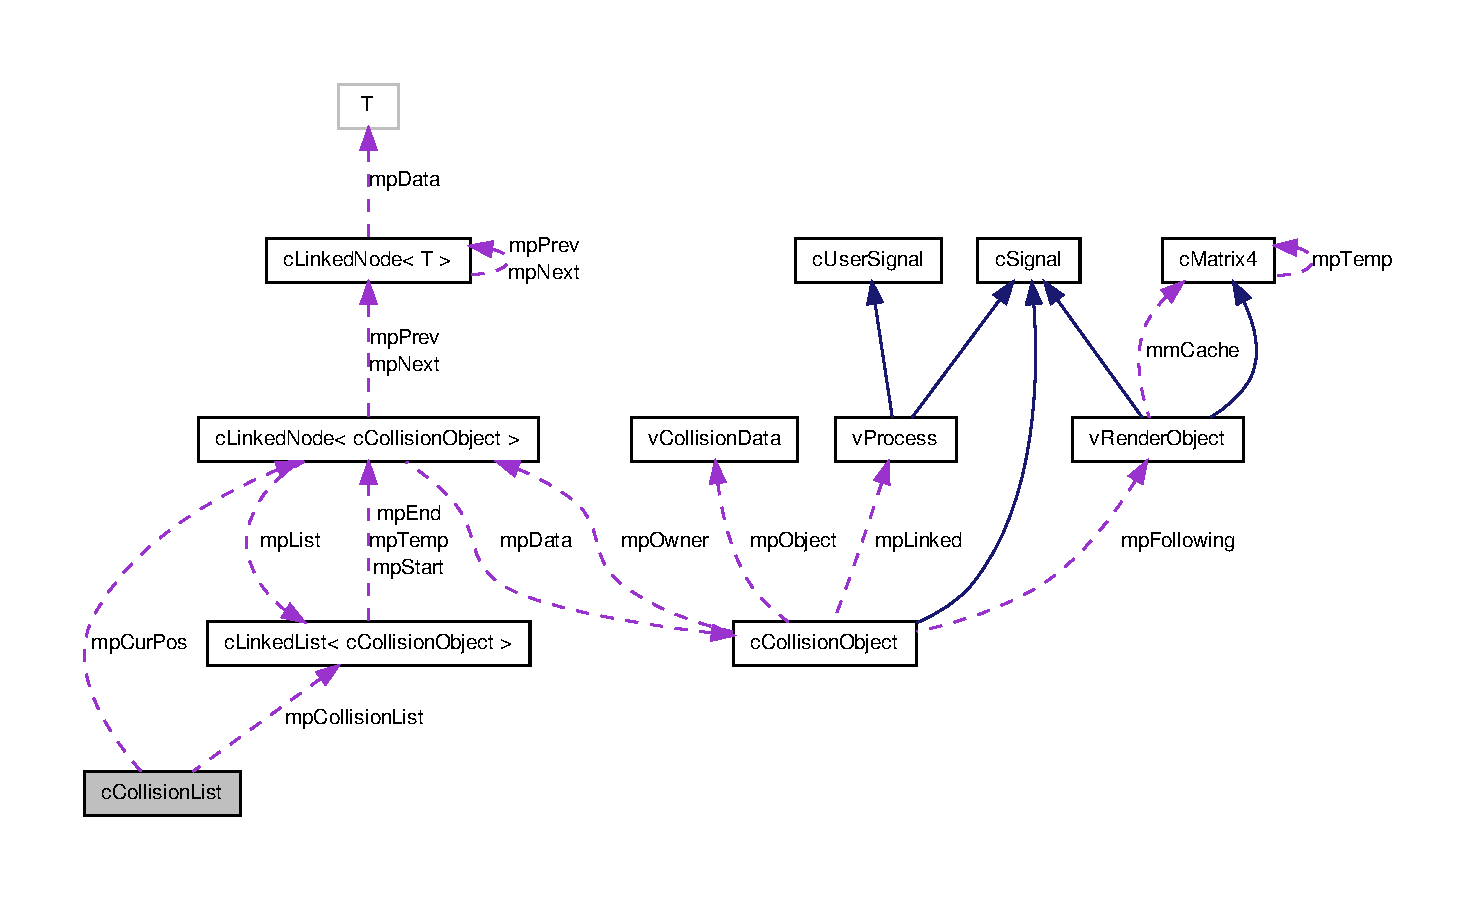
\includegraphics[width=400pt]{classc_collision_list__coll__graph}
\end{center}
\end{figure}
\subsection*{Public Member Functions}
\begin{DoxyCompactItemize}
\item 
\hypertarget{classc_collision_list_a1b84b682ec105262682532b0a90754c2}{
\hyperlink{classc_collision_list_a1b84b682ec105262682532b0a90754c2}{cCollisionList} ()}
\label{classc_collision_list_a1b84b682ec105262682532b0a90754c2}

\begin{DoxyCompactList}\small\item\em The Constructor for \hyperlink{classc_collision_list}{cCollisionList}. \end{DoxyCompactList}\item 
\hypertarget{classc_collision_list_ace525d10fc1a38477cee11e14714b476}{
void \hyperlink{classc_collision_list_ace525d10fc1a38477cee11e14714b476}{AddCollision} (\hyperlink{classc_collision_object}{cCollisionObject} $\ast$lpObject)}
\label{classc_collision_list_ace525d10fc1a38477cee11e14714b476}

\begin{DoxyCompactList}\small\item\em This will Add the object lpObject to the list of objects colliding with the current searching object. \end{DoxyCompactList}\item 
\hypertarget{classc_collision_list_adeef80e9e181e81dc073ebcfa1d8bec4}{
\hyperlink{classc_collision_object}{cCollisionObject} $\ast$ \hyperlink{classc_collision_list_adeef80e9e181e81dc073ebcfa1d8bec4}{NextCollisionItem} ()}
\label{classc_collision_list_adeef80e9e181e81dc073ebcfa1d8bec4}

\begin{DoxyCompactList}\small\item\em This will return the next item from the list mpCollisionList that has been stocked by GenerateCollisionList() as a CollisionObject pointer. \end{DoxyCompactList}\item 
\hypertarget{classc_collision_list_ac641346bbc7e3d3b84880ae03b0496c5}{
\hyperlink{classc_process}{cProcess} $\ast$ \hyperlink{classc_collision_list_ac641346bbc7e3d3b84880ae03b0496c5}{NextCollisionP} ()}
\label{classc_collision_list_ac641346bbc7e3d3b84880ae03b0496c5}

\begin{DoxyCompactList}\small\item\em This will return the process owning renderable object creating the next detected collision. \end{DoxyCompactList}\item 
\hypertarget{classc_collision_list_a87c8ee3baa85ff002030c83bd1784192}{
vRenderObject $\ast$ \hyperlink{classc_collision_list_a87c8ee3baa85ff002030c83bd1784192}{NextCollisionR} ()}
\label{classc_collision_list_a87c8ee3baa85ff002030c83bd1784192}

\begin{DoxyCompactList}\small\item\em This will return the renderable object involved in the next detected collision. \end{DoxyCompactList}\item 
\hypertarget{classc_collision_list_ac04316a4e8d0e3c5c3213c20bd7897cc}{
void \hyperlink{classc_collision_list_ac04316a4e8d0e3c5c3213c20bd7897cc}{ResetList} ()}
\label{classc_collision_list_ac04316a4e8d0e3c5c3213c20bd7897cc}

\begin{DoxyCompactList}\small\item\em This will reset the collision search to the start of mpList. \end{DoxyCompactList}\item 
\hypertarget{classc_collision_list_a628ed6510cd89c192a402be0a64ea111}{
\hyperlink{classc_collision_list_a628ed6510cd89c192a402be0a64ea111}{$\sim$cCollisionList} ()}
\label{classc_collision_list_a628ed6510cd89c192a402be0a64ea111}

\begin{DoxyCompactList}\small\item\em This is the destructor for \hyperlink{classc_collision_list}{cCollisionList}. \end{DoxyCompactList}\item 
\hypertarget{classc_collision_list_ae279c0239ead11e2d6c3647495347cc4}{
void \hyperlink{classc_collision_list_ae279c0239ead11e2d6c3647495347cc4}{SortByDistance} ()}
\label{classc_collision_list_ae279c0239ead11e2d6c3647495347cc4}

\begin{DoxyCompactList}\small\item\em This will sort the list of collisionobjects into distance from the colliding object order. This allows the user to resolve the collisions in 'Chronological' order. \end{DoxyCompactList}\end{DoxyCompactItemize}


\subsection{Detailed Description}
This is generated by doing Collision Detection with an object. This will cache all the detected collisions with the object used for the collision detection. This allows the user to access the collisions in a different order to the order they were detected or to cache it for use later. The list is composed of a list of \hyperlink{classc_collision_list_object}{cCollisionListObject}. 
\hypertarget{classc_collision_list_object}{
\section{cCollisionListObject Class Reference}
\label{classc_collision_list_object}\index{cCollisionListObject@{cCollisionListObject}}
}


Collaboration diagram for cCollisionListObject:
\nopagebreak
\begin{figure}[H]
\begin{center}
\leavevmode
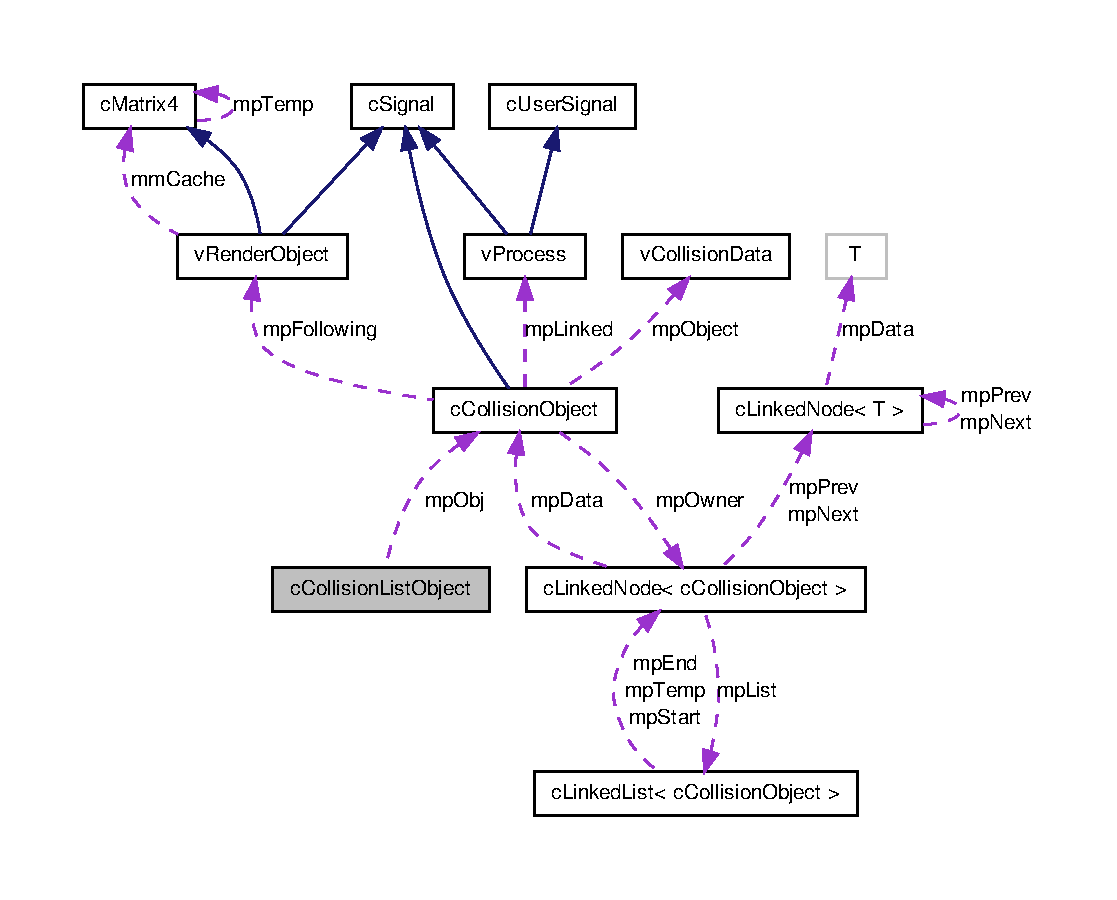
\includegraphics[width=400pt]{classc_collision_list_object__coll__graph}
\end{center}
\end{figure}
\subsection*{Public Member Functions}
\begin{DoxyCompactItemize}
\item 
\hyperlink{classc_collision_list_object_a08d25f1e82853098b07ad9c30c8b21a8}{cCollisionListObject} (\hyperlink{classc_collision_object}{cCollisionObject} $\ast$lpObj)
\item 
float \hyperlink{classc_collision_list_object_a1f78164f5389c06744a447c9caf86372}{GetDistance} ()
\end{DoxyCompactItemize}


\subsection{Detailed Description}


Definition at line 4 of file WTcCollisionList.h.



\subsection{Constructor \& Destructor Documentation}
\hypertarget{classc_collision_list_object_a08d25f1e82853098b07ad9c30c8b21a8}{
\index{cCollisionListObject@{cCollisionListObject}!cCollisionListObject@{cCollisionListObject}}
\index{cCollisionListObject@{cCollisionListObject}!cCollisionListObject@{cCollisionListObject}}
\subsubsection[{cCollisionListObject}]{\setlength{\rightskip}{0pt plus 5cm}cCollisionListObject::cCollisionListObject (
\begin{DoxyParamCaption}
\item[{{\bf cCollisionObject} $\ast$}]{lpObj}
\end{DoxyParamCaption}
)\hspace{0.3cm}{\ttfamily  \mbox{[}inline\mbox{]}}}}
\label{classc_collision_list_object_a08d25f1e82853098b07ad9c30c8b21a8}


Definition at line 9 of file WTcCollisionList.h.



\subsection{Member Function Documentation}
\hypertarget{classc_collision_list_object_a1f78164f5389c06744a447c9caf86372}{
\index{cCollisionListObject@{cCollisionListObject}!GetDistance@{GetDistance}}
\index{GetDistance@{GetDistance}!cCollisionListObject@{cCollisionListObject}}
\subsubsection[{GetDistance}]{\setlength{\rightskip}{0pt plus 5cm}float cCollisionListObject::GetDistance (
\begin{DoxyParamCaption}
{}
\end{DoxyParamCaption}
)\hspace{0.3cm}{\ttfamily  \mbox{[}inline\mbox{]}}}}
\label{classc_collision_list_object_a1f78164f5389c06744a447c9caf86372}


Definition at line 10 of file WTcCollisionList.h.


\hypertarget{classc_collision_object}{
\section{cCollisionObject Class Reference}
\label{classc_collision_object}\index{cCollisionObject@{cCollisionObject}}
}


Inheritance diagram for cCollisionObject:
\nopagebreak
\begin{figure}[H]
\begin{center}
\leavevmode
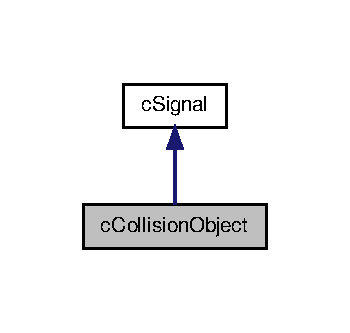
\includegraphics[width=168pt]{classc_collision_object__inherit__graph}
\end{center}
\end{figure}


Collaboration diagram for cCollisionObject:
\nopagebreak
\begin{figure}[H]
\begin{center}
\leavevmode
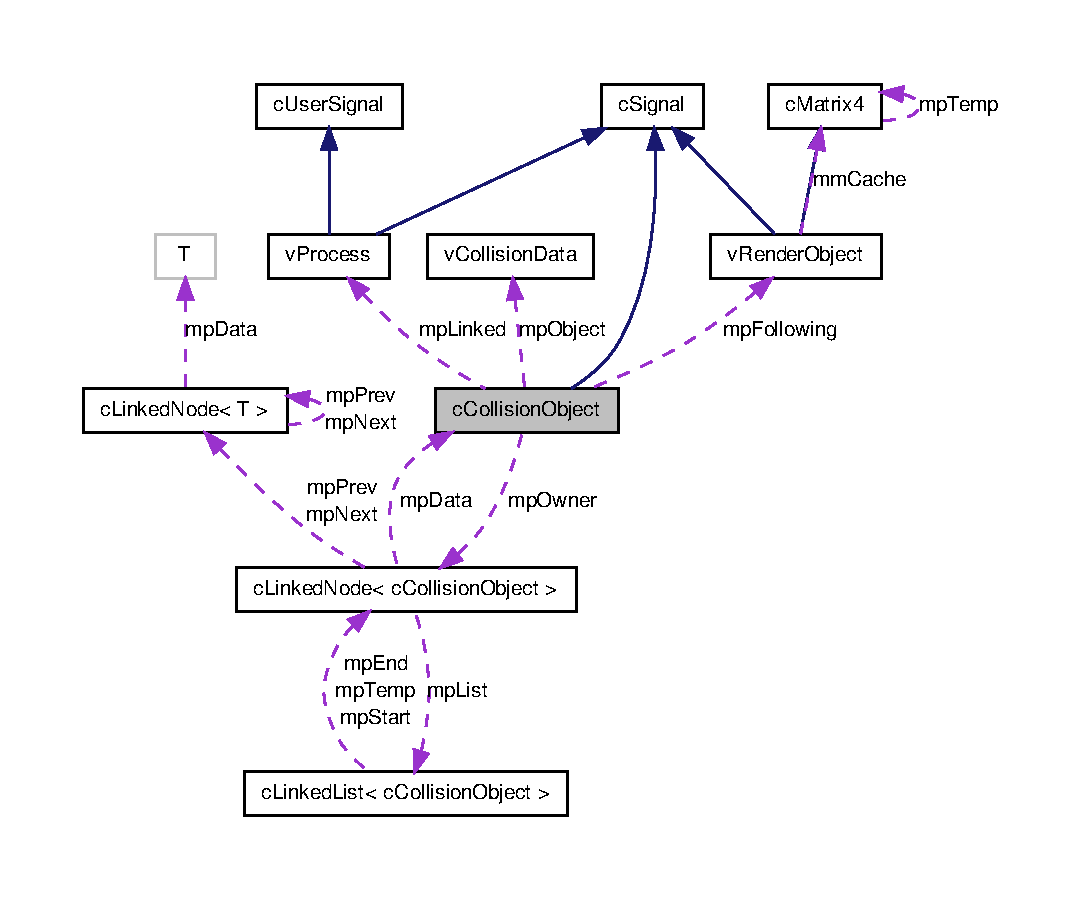
\includegraphics[width=400pt]{classc_collision_object__coll__graph}
\end{center}
\end{figure}
\subsection*{Public Member Functions}
\begin{DoxyCompactItemize}
\item 
\hyperlink{classc_collision_object_a90f4a7fe0445396ddf49e14bda27f2dc}{cCollisionObject} (\hyperlink{classv_render_object}{vRenderObject} $\ast$lpFollow, \hyperlink{classv_process}{vProcess} $\ast$lpLinked=0, uint32 liFilterType=0)
\item 
\hyperlink{classc_collision_object_a38fc1abcd7a0f240d7ce41aca108bb43}{cCollisionObject} (\hyperlink{classc_beam_mesh}{cBeamMesh} $\ast$lpFollow, \hyperlink{classv_process}{vProcess} $\ast$lpLinked=0, uint32 liFilterType=0)
\item 
void \hyperlink{classc_collision_object_a4aaae58a85bd7c1e6b5601a4e4cac3c1}{Initialise} (\hyperlink{classv_render_object}{vRenderObject} $\ast$lpFollow, \hyperlink{classv_process}{vProcess} $\ast$lpLinked, uint32 liFilterType)
\item 
\hyperlink{classc_collision_object_ac01e53c6dadd3ab8036f485b9115aedd}{$\sim$cCollisionObject} ()
\item 
bool \hyperlink{classc_collision_object_ac56988f3641d39409fbf4ccba3525282}{CreatedThisFrame} ()
\item 
void \hyperlink{classc_collision_object_a31156a5bfff63de45daa32893a30697c}{NotCreatedThisFrame} ()
\item 
\hyperlink{classv_collision_data}{vCollisionData} $\ast$ \hyperlink{classc_collision_object_a58a3680126c2d7e405ec80402cb8208e}{CollisionData} ()
\item 
void \hyperlink{classc_collision_object_abec1a68ab54f2e80244c8b336bca3626}{Signal} (SIGNAL liFlags)
\begin{DoxyCompactList}\small\item\em This is the function that will handle a system signal. Possible signals to be passed in are \_\-S\_\-SLEEP,\_\-S\_\-WAKE,\_\-S\_\-KILL,\_\-S\_\-SLEEP\_\-TREE, \_\-S\_\-WAKE\_\-TREE,\_\-S\_\-KILL\_\-TREE. \item\end{DoxyCompactList}\item 
bool \hyperlink{classc_collision_object_a9d4e4fe61df1af3479247611d605e897}{Procedural} ()
\item 
bool \hyperlink{classc_collision_object_a695516ede632cf0e02ddbcd7b6e539a7}{Loaded} ()
\item 
void \hyperlink{classc_collision_object_a908a1cbe39b07c53849f60fecb5230dc}{ClearProcedural} ()
\item 
\hyperlink{classc_sphere_collision}{cSphereCollision} $\ast$ \hyperlink{classc_collision_object_afe43e12c0ea0da5c3653450cb8dfb047}{Sphere} ()
\item 
\hyperlink{classc_mesh_collision}{cMeshCollision} $\ast$ \hyperlink{classc_collision_object_a6ea07e3f2501b7092fed0130f150c4f4}{Mesh} ()
\item 
\hyperlink{classc_ray_collision}{cRayCollision} $\ast$ \hyperlink{classc_collision_object_ac46982867551f6dd05c0dbcae0e57796}{Ray} ()
\item 
\hyperlink{classc_beam_collision}{cBeamCollision} $\ast$ \hyperlink{classc_collision_object_a8a5a6900686ac3ac88cf6bdac71569ad}{Beam} ()
\item 
void \hyperlink{classc_collision_object_ae465362052ff2026ed31c2fa3664d209}{SetType} (\hyperlink{classc_sphere_collision}{cSphereCollision} $\ast$lpSphere)
\begin{DoxyCompactList}\small\item\em This will take a SphereCollision Object loaded from a file, and set this Collision Object to use it. \item\end{DoxyCompactList}\item 
void \hyperlink{classc_collision_object_a5c46dea7134fa466293938c22a780529}{SetType} (\hyperlink{classc_mesh_collision}{cMeshCollision} $\ast$lpMesh)
\begin{DoxyCompactList}\small\item\em This will take a MeshCollision Object loaded from a file, and set this Collision Object to use it. \item\end{DoxyCompactList}\item 
void \hyperlink{classc_collision_object_a4282627cb1818f66842f3c8ff91cd20e}{SetType} (\hyperlink{classc_beam_collision}{cBeamCollision} $\ast$lpBeam)
\begin{DoxyCompactList}\small\item\em This will take a BeamCollision Object loaded from a file, and set this Collision Object to use it. \item\end{DoxyCompactList}\item 
void \hyperlink{classc_collision_object_a8ef73a19857e4a35470502776b0f03f8}{OnFile} (\hyperlink{classv_collision_data}{vCollisionData} $\ast$lpPoint)
\item 
void \hyperlink{classc_collision_object_a6ea3e10f69f7a2d5cae2bd4471461137}{OnProcedural} ()
\item 
\hyperlink{classc_sphere_collision}{cSphereCollision} $\ast$ \hyperlink{classc_collision_object_a22e6f4f5c722b6d45629d92488e5d925}{SetType} (float lfSize)
\begin{DoxyCompactList}\small\item\em This will procedurally generate a Sphere or radius 1.0f;. \item\end{DoxyCompactList}\item 
\hyperlink{classc_beam_collision}{cBeamCollision} $\ast$ \hyperlink{classc_collision_object_ab5fc1f36d50ea87a69b4879076a92533}{SetType} (float lfLength, float lfRadius)
\begin{DoxyCompactList}\small\item\em This will procedurally generate a Beam of Radius lfRadius and Length lfLength. \item\end{DoxyCompactList}\item 
\hyperlink{classc_mesh_collision}{cMeshCollision} $\ast$ \hyperlink{classc_collision_object_a40b80411356222997bb94fae10796c93}{SetType} (float $\ast$lpBounds)
\begin{DoxyCompactList}\small\item\em This will procedureally generate a Box collision object from the array of 6 floats lpBounds. see cGeneratedBoxCollision::BuildObject(float $\ast$lpBounds) for more information. \item\end{DoxyCompactList}\item 
\hyperlink{classc_ray_collision}{cRayCollision} $\ast$ \hyperlink{classc_collision_object_a761dae3de0ea58d4d60b98348177b7ed}{SetType} (\hyperlink{classc_render_object}{cRenderObject} $\ast$lpObj)
\begin{DoxyCompactList}\small\item\em This will make a ray object. See cRayCollision::BuildObject(float $\ast$lpBounds) for more information. Makes Ray radius to be same as object and ray to follow it's movement. \item\end{DoxyCompactList}\item 
\hyperlink{classc_beam_collision}{cBeamCollision} $\ast$ \hyperlink{classc_collision_object_a0d08a63b8b7a3bcf6eb1c6617ec71e91}{SetType} (\hyperlink{classc_beam_mesh}{cBeamMesh} $\ast$lpBeam)
\begin{DoxyCompactList}\small\item\em This will make a Beam object to match a rendered Beam. (Nice and easy eh?) \item\end{DoxyCompactList}\item 
\hyperlink{classc_sphere_collision}{cSphereCollision} $\ast$ \hyperlink{classc_collision_object_add80d08291b6c162bdf9b5f7408d6617}{GetCollisionData} ()
\item 
uint8 \hyperlink{classc_collision_object_ae1274b9a69dfa081cda23a840c9e2df4}{Type} ()
\begin{DoxyCompactList}\small\item\em This is the accurate way of determining the type of these objects. \item\end{DoxyCompactList}\item 
bool \hyperlink{classc_collision_object_a6f5b5341a726cb0a54fe3271b110dc8c}{CheckCollision} (\hyperlink{classc_collision_object}{cCollisionObject} $\ast$lpOther)
\begin{DoxyCompactList}\small\item\em This will check for a collision between this object and the object lpOther. \item\end{DoxyCompactList}\item 
bool \hyperlink{classc_collision_object_a1d93858e03da25f8656ae688c4dedbce}{TouchCollision} (\hyperlink{classc_collision_object}{cCollisionObject} $\ast$lpOther)
\item 
\hyperlink{classc_matrix4}{cMatrix4} \& \hyperlink{classc_collision_object_abc47ab584910cc877b5e723be4e09eac}{CacheMatrix} ()
\begin{DoxyCompactList}\small\item\em This will return the Objects Cached Matrix mmCache. \item\end{DoxyCompactList}\item 
\hyperlink{classv_render_object}{vRenderObject} $\ast$ \hyperlink{classc_collision_object_a959994c60b68de6be85dcc663228bab8}{RenderObject} ()
\begin{DoxyCompactList}\small\item\em This will return a pointer the \hyperlink{classc_render_object}{cRenderObject} linked to this. \item\end{DoxyCompactList}\item 
uint32 \hyperlink{classc_collision_object_a1490cdf75c8037049bfa7891aa8756b7}{CollisionFilter} ()
\begin{DoxyCompactList}\small\item\em This will return the current Collision Filter ID of this object. \item\end{DoxyCompactList}\item 
void \hyperlink{classc_collision_object_a2a527f445a899adafbf18dddf140e179}{CollisionFilter} (uint32 liID)
\begin{DoxyCompactList}\small\item\em This will set the Collision Filter ID of this object. \item\end{DoxyCompactList}\item 
bool \hyperlink{classc_collision_object_ae9f62c64221d8cc347010fed3cf6e8d1}{Collision} (\hyperlink{classc_collision_object}{cCollisionObject} $\ast$lpOther, uint32 lpCol)
\item 
bool \hyperlink{classc_collision_object_abf62376a5806d878b5810acfd40bc450}{Collision} (\hyperlink{classc_collision_object}{cCollisionObject} $\ast$lpOther)
\item 
bool \hyperlink{classc_collision_object_acc8e58a747eba8e5c7903c8d769b9b31}{CompareRanges} (float lf1, float lf2, float lfR)
\begin{DoxyCompactList}\small\item\em This will do a sphere collision between two points. lf1 and lf2 are x$\ast$x+y$\ast$y+z$\ast$z. lfR is (Sum of Radii)$\ast$(Sum of Radii). \item\end{DoxyCompactList}\item 
void \hyperlink{classc_collision_object_a30475084c3b15f9bf8dc8818ed486c7d}{SetLink} (\hyperlink{classv_process}{vProcess} $\ast$lpLink)
\begin{DoxyCompactList}\small\item\em This sets the process that this renderable object will return collision signals to. \item\end{DoxyCompactList}\item 
\hyperlink{classv_process}{vProcess} $\ast$ \hyperlink{classc_collision_object_a7b501c8848f32131eb36b1f7f69c21ec}{GetLink} ()
\begin{DoxyCompactList}\small\item\em Returns the process currently linked to this renderable object. \item\end{DoxyCompactList}\item 
void \hyperlink{classc_collision_object_a40afa697b7e09e716b471725e6e33805}{GenerateCollisionList} (uint32 liType=0)
\begin{DoxyCompactList}\small\item\em This will generate a collision list of all objects colliding with this object filtered by type liType. \item\end{DoxyCompactList}\item 
float $\ast$ \hyperlink{classc_collision_object_a66f5ab6f3e5b3d618625b8c254f477ab}{GetPos} ()
\begin{DoxyCompactList}\small\item\em This will return the position of the selected object. \item\end{DoxyCompactList}\item 
void \hyperlink{classc_collision_object_a86932ba04099dd34874fd3ada314168c}{PreUpdateCache} ()
\begin{DoxyCompactList}\small\item\em This will remove the \hyperlink{classc_collision_object}{cCollisionObject} from it's Spatial Slots before its position is updated. \item\end{DoxyCompactList}\item 
void \hyperlink{classc_collision_object_a7719840f3fcc5bf3dcef08d123066739}{PostUpdateCache} ()
\begin{DoxyCompactList}\small\item\em This will Add the \hyperlink{classc_collision_object}{cCollisionObject} to the relevant Spatial Slots after it has found it's new position. \item\end{DoxyCompactList}\item 
bool \hyperlink{classc_collision_object_a53623f53b0ac497bfa1c794a76d2f818}{SphereSphere} (\hyperlink{classc_collision_object}{cCollisionObject} $\ast$lpOther)
\item 
bool \hyperlink{classc_collision_object_ae87264d7ecd143a67244c95b10c07ab7}{ModelModel} (\hyperlink{classc_collision_object}{cCollisionObject} $\ast$lpOther)
\item 
bool \hyperlink{classc_collision_object_aa4500b5834736e5abeabe71c300e64e8}{RayRay} (\hyperlink{classc_collision_object}{cCollisionObject} $\ast$lpOther)
\item 
bool \hyperlink{classc_collision_object_a299e49b5d78e1e7dbe5e801c7760462a}{SphereModel} (\hyperlink{classc_collision_object}{cCollisionObject} $\ast$lpOther)
\item 
bool \hyperlink{classc_collision_object_ae4761ec4a0f60667e83cb6d4cf39d359}{SphereRay} (\hyperlink{classc_collision_object}{cCollisionObject} $\ast$lpOther)
\item 
bool \hyperlink{classc_collision_object_a7ccea939e1f91fa7eeda4c31128901c3}{RayModel} (\hyperlink{classc_collision_object}{cCollisionObject} $\ast$lpOther)
\item 
float \hyperlink{classc_collision_object_ae6c320e7a3361fbbc4796463d777daab}{GetCollisionSize} ()
\end{DoxyCompactItemize}
\subsection*{Static Public Attributes}
\begin{DoxyCompactItemize}
\item 
static float \hyperlink{classc_collision_object_a3afac28cfda77f7ed63605e604c1139a}{mfStaticSize} \mbox{[}3\mbox{]} = \{0.0f,0.0f,0.0f\}
\begin{DoxyCompactList}\small\item\em This is a temporary storage for transfering sizes between objects. \item\end{DoxyCompactList}\end{DoxyCompactItemize}


\subsection{Detailed Description}


Definition at line 14 of file WTcCollisionObject.h.



\subsection{Constructor \& Destructor Documentation}
\hypertarget{classc_collision_object_a90f4a7fe0445396ddf49e14bda27f2dc}{
\index{cCollisionObject@{cCollisionObject}!cCollisionObject@{cCollisionObject}}
\index{cCollisionObject@{cCollisionObject}!cCollisionObject@{cCollisionObject}}
\subsubsection[{cCollisionObject}]{\setlength{\rightskip}{0pt plus 5cm}cCollisionObject::cCollisionObject (
\begin{DoxyParamCaption}
\item[{{\bf vRenderObject} $\ast$}]{lpFollow, }
\item[{{\bf vProcess} $\ast$}]{lpLinked = {\ttfamily 0}, }
\item[{uint32}]{liFilterType = {\ttfamily 0}}
\end{DoxyParamCaption}
)}}
\label{classc_collision_object_a90f4a7fe0445396ddf49e14bda27f2dc}


Definition at line 839 of file WTcCollisionObject.cpp.

\hypertarget{classc_collision_object_a38fc1abcd7a0f240d7ce41aca108bb43}{
\index{cCollisionObject@{cCollisionObject}!cCollisionObject@{cCollisionObject}}
\index{cCollisionObject@{cCollisionObject}!cCollisionObject@{cCollisionObject}}
\subsubsection[{cCollisionObject}]{\setlength{\rightskip}{0pt plus 5cm}cCollisionObject::cCollisionObject (
\begin{DoxyParamCaption}
\item[{{\bf cBeamMesh} $\ast$}]{lpFollow, }
\item[{{\bf vProcess} $\ast$}]{lpLinked = {\ttfamily 0}, }
\item[{uint32}]{liFilterType = {\ttfamily 0}}
\end{DoxyParamCaption}
)}}
\label{classc_collision_object_a38fc1abcd7a0f240d7ce41aca108bb43}


Definition at line 856 of file WTcCollisionObject.cpp.

\hypertarget{classc_collision_object_ac01e53c6dadd3ab8036f485b9115aedd}{
\index{cCollisionObject@{cCollisionObject}!$\sim$cCollisionObject@{$\sim$cCollisionObject}}
\index{$\sim$cCollisionObject@{$\sim$cCollisionObject}!cCollisionObject@{cCollisionObject}}
\subsubsection[{$\sim$cCollisionObject}]{\setlength{\rightskip}{0pt plus 5cm}cCollisionObject::$\sim$cCollisionObject (
\begin{DoxyParamCaption}
{}
\end{DoxyParamCaption}
)}}
\label{classc_collision_object_ac01e53c6dadd3ab8036f485b9115aedd}


Definition at line 754 of file WTcCollisionObject.cpp.



\subsection{Member Function Documentation}
\hypertarget{classc_collision_object_a8a5a6900686ac3ac88cf6bdac71569ad}{
\index{cCollisionObject@{cCollisionObject}!Beam@{Beam}}
\index{Beam@{Beam}!cCollisionObject@{cCollisionObject}}
\subsubsection[{Beam}]{\setlength{\rightskip}{0pt plus 5cm}{\bf cBeamCollision}$\ast$ cCollisionObject::Beam (
\begin{DoxyParamCaption}
{}
\end{DoxyParamCaption}
)\hspace{0.3cm}{\ttfamily  \mbox{[}inline\mbox{]}}}}
\label{classc_collision_object_a8a5a6900686ac3ac88cf6bdac71569ad}
This is a dynamic cast on the type of collision object this is. Note ALL cCollisionData objects return true to Sphere. This applies to all the functions \hyperlink{classc_collision_object_afe43e12c0ea0da5c3653450cb8dfb047}{Sphere()},Box(),\hyperlink{classc_collision_object_a6ea07e3f2501b7092fed0130f150c4f4}{Mesh()},\hyperlink{classc_collision_object_ac46982867551f6dd05c0dbcae0e57796}{Ray()} and \hyperlink{classc_collision_object_a8a5a6900686ac3ac88cf6bdac71569ad}{Beam()}. 

Definition at line 74 of file WTcCollisionObject.h.

\hypertarget{classc_collision_object_abc47ab584910cc877b5e723be4e09eac}{
\index{cCollisionObject@{cCollisionObject}!CacheMatrix@{CacheMatrix}}
\index{CacheMatrix@{CacheMatrix}!cCollisionObject@{cCollisionObject}}
\subsubsection[{CacheMatrix}]{\setlength{\rightskip}{0pt plus 5cm}{\bf cMatrix4}\& cCollisionObject::CacheMatrix (
\begin{DoxyParamCaption}
{}
\end{DoxyParamCaption}
)\hspace{0.3cm}{\ttfamily  \mbox{[}inline\mbox{]}}}}
\label{classc_collision_object_abc47ab584910cc877b5e723be4e09eac}


This will return the Objects Cached Matrix mmCache. 



Definition at line 142 of file WTcCollisionObject.h.

\hypertarget{classc_collision_object_a6f5b5341a726cb0a54fe3271b110dc8c}{
\index{cCollisionObject@{cCollisionObject}!CheckCollision@{CheckCollision}}
\index{CheckCollision@{CheckCollision}!cCollisionObject@{cCollisionObject}}
\subsubsection[{CheckCollision}]{\setlength{\rightskip}{0pt plus 5cm}bool cCollisionObject::CheckCollision (
\begin{DoxyParamCaption}
\item[{{\bf cCollisionObject} $\ast$}]{lpOther}
\end{DoxyParamCaption}
)}}
\label{classc_collision_object_a6f5b5341a726cb0a54fe3271b110dc8c}


This will check for a collision between this object and the object lpOther. 

$\ast$ 
\begin{DoxyParams}{Parameters}
{\em lpOther} & is a pointer to the other collision object to check against. It will check both objects have collisions on. Then it will do an initial quick check to see if a collision is a possibility. Finally if required it will do a much more detailed collision check. \\
\hline
\end{DoxyParams}


Definition at line 673 of file WTcCollisionObject.cpp.

\hypertarget{classc_collision_object_a908a1cbe39b07c53849f60fecb5230dc}{
\index{cCollisionObject@{cCollisionObject}!ClearProcedural@{ClearProcedural}}
\index{ClearProcedural@{ClearProcedural}!cCollisionObject@{cCollisionObject}}
\subsubsection[{ClearProcedural}]{\setlength{\rightskip}{0pt plus 5cm}void cCollisionObject::ClearProcedural (
\begin{DoxyParamCaption}
{}
\end{DoxyParamCaption}
)}}
\label{classc_collision_object_a908a1cbe39b07c53849f60fecb5230dc}


Definition at line 871 of file WTcCollisionObject.cpp.

\hypertarget{classc_collision_object_abf62376a5806d878b5810acfd40bc450}{
\index{cCollisionObject@{cCollisionObject}!Collision@{Collision}}
\index{Collision@{Collision}!cCollisionObject@{cCollisionObject}}
\subsubsection[{Collision}]{\setlength{\rightskip}{0pt plus 5cm}bool cCollisionObject::Collision (
\begin{DoxyParamCaption}
\item[{{\bf cCollisionObject} $\ast$}]{lpOther}
\end{DoxyParamCaption}
)}}
\label{classc_collision_object_abf62376a5806d878b5810acfd40bc450}


Definition at line 665 of file WTcCollisionObject.cpp.

\hypertarget{classc_collision_object_ae9f62c64221d8cc347010fed3cf6e8d1}{
\index{cCollisionObject@{cCollisionObject}!Collision@{Collision}}
\index{Collision@{Collision}!cCollisionObject@{cCollisionObject}}
\subsubsection[{Collision}]{\setlength{\rightskip}{0pt plus 5cm}bool cCollisionObject::Collision (
\begin{DoxyParamCaption}
\item[{{\bf cCollisionObject} $\ast$}]{lpOther, }
\item[{uint32}]{lpCol}
\end{DoxyParamCaption}
)}}
\label{classc_collision_object_ae9f62c64221d8cc347010fed3cf6e8d1}
This Function will control the collision detection between this object and lpOther. It will check the filter lpCol to cehck that the other object is of a suitable type. Then will call \hyperlink{classc_collision_object_a6f5b5341a726cb0a54fe3271b110dc8c}{CheckCollision(cCollisionObject $\ast$lpOther)} 

Definition at line 654 of file WTcCollisionObject.cpp.

\hypertarget{classc_collision_object_a58a3680126c2d7e405ec80402cb8208e}{
\index{cCollisionObject@{cCollisionObject}!CollisionData@{CollisionData}}
\index{CollisionData@{CollisionData}!cCollisionObject@{cCollisionObject}}
\subsubsection[{CollisionData}]{\setlength{\rightskip}{0pt plus 5cm}{\bf vCollisionData}$\ast$ cCollisionObject::CollisionData (
\begin{DoxyParamCaption}
{}
\end{DoxyParamCaption}
)\hspace{0.3cm}{\ttfamily  \mbox{[}inline\mbox{]}}}}
\label{classc_collision_object_a58a3680126c2d7e405ec80402cb8208e}


Definition at line 53 of file WTcCollisionObject.h.

\hypertarget{classc_collision_object_a1490cdf75c8037049bfa7891aa8756b7}{
\index{cCollisionObject@{cCollisionObject}!CollisionFilter@{CollisionFilter}}
\index{CollisionFilter@{CollisionFilter}!cCollisionObject@{cCollisionObject}}
\subsubsection[{CollisionFilter}]{\setlength{\rightskip}{0pt plus 5cm}uint32 cCollisionObject::CollisionFilter (
\begin{DoxyParamCaption}
{}
\end{DoxyParamCaption}
)\hspace{0.3cm}{\ttfamily  \mbox{[}inline\mbox{]}}}}
\label{classc_collision_object_a1490cdf75c8037049bfa7891aa8756b7}


This will return the current Collision Filter ID of this object. 



Definition at line 152 of file WTcCollisionObject.h.

\hypertarget{classc_collision_object_a2a527f445a899adafbf18dddf140e179}{
\index{cCollisionObject@{cCollisionObject}!CollisionFilter@{CollisionFilter}}
\index{CollisionFilter@{CollisionFilter}!cCollisionObject@{cCollisionObject}}
\subsubsection[{CollisionFilter}]{\setlength{\rightskip}{0pt plus 5cm}void cCollisionObject::CollisionFilter (
\begin{DoxyParamCaption}
\item[{uint32}]{liID}
\end{DoxyParamCaption}
)}}
\label{classc_collision_object_a2a527f445a899adafbf18dddf140e179}


This will set the Collision Filter ID of this object. 



Definition at line 616 of file WTcCollisionObject.cpp.

\hypertarget{classc_collision_object_acc8e58a747eba8e5c7903c8d769b9b31}{
\index{cCollisionObject@{cCollisionObject}!CompareRanges@{CompareRanges}}
\index{CompareRanges@{CompareRanges}!cCollisionObject@{cCollisionObject}}
\subsubsection[{CompareRanges}]{\setlength{\rightskip}{0pt plus 5cm}bool cCollisionObject::CompareRanges (
\begin{DoxyParamCaption}
\item[{float}]{lf1, }
\item[{float}]{lf2, }
\item[{float}]{lfR}
\end{DoxyParamCaption}
)}}
\label{classc_collision_object_acc8e58a747eba8e5c7903c8d769b9b31}


This will do a sphere collision between two points. lf1 and lf2 are x$\ast$x+y$\ast$y+z$\ast$z. lfR is (Sum of Radii)$\ast$(Sum of Radii). 

\hypertarget{classc_collision_object_ac56988f3641d39409fbf4ccba3525282}{
\index{cCollisionObject@{cCollisionObject}!CreatedThisFrame@{CreatedThisFrame}}
\index{CreatedThisFrame@{CreatedThisFrame}!cCollisionObject@{cCollisionObject}}
\subsubsection[{CreatedThisFrame}]{\setlength{\rightskip}{0pt plus 5cm}bool cCollisionObject::CreatedThisFrame (
\begin{DoxyParamCaption}
{}
\end{DoxyParamCaption}
)\hspace{0.3cm}{\ttfamily  \mbox{[}inline\mbox{]}}}}
\label{classc_collision_object_ac56988f3641d39409fbf4ccba3525282}


Definition at line 49 of file WTcCollisionObject.h.

\hypertarget{classc_collision_object_a40afa697b7e09e716b471725e6e33805}{
\index{cCollisionObject@{cCollisionObject}!GenerateCollisionList@{GenerateCollisionList}}
\index{GenerateCollisionList@{GenerateCollisionList}!cCollisionObject@{cCollisionObject}}
\subsubsection[{GenerateCollisionList}]{\setlength{\rightskip}{0pt plus 5cm}void cCollisionObject::GenerateCollisionList (
\begin{DoxyParamCaption}
\item[{uint32}]{liType = {\ttfamily 0}}
\end{DoxyParamCaption}
)}}
\label{classc_collision_object_a40afa697b7e09e716b471725e6e33805}


This will generate a collision list of all objects colliding with this object filtered by type liType. 



Definition at line 605 of file WTcCollisionObject.cpp.

\hypertarget{classc_collision_object_add80d08291b6c162bdf9b5f7408d6617}{
\index{cCollisionObject@{cCollisionObject}!GetCollisionData@{GetCollisionData}}
\index{GetCollisionData@{GetCollisionData}!cCollisionObject@{cCollisionObject}}
\subsubsection[{GetCollisionData}]{\setlength{\rightskip}{0pt plus 5cm}{\bf cSphereCollision}$\ast$ cCollisionObject::GetCollisionData (
\begin{DoxyParamCaption}
{}
\end{DoxyParamCaption}
)\hspace{0.3cm}{\ttfamily  \mbox{[}inline\mbox{]}}}}
\label{classc_collision_object_add80d08291b6c162bdf9b5f7408d6617}


Definition at line 97 of file WTcCollisionObject.h.

\hypertarget{classc_collision_object_ae6c320e7a3361fbbc4796463d777daab}{
\index{cCollisionObject@{cCollisionObject}!GetCollisionSize@{GetCollisionSize}}
\index{GetCollisionSize@{GetCollisionSize}!cCollisionObject@{cCollisionObject}}
\subsubsection[{GetCollisionSize}]{\setlength{\rightskip}{0pt plus 5cm}float cCollisionObject::GetCollisionSize (
\begin{DoxyParamCaption}
{}
\end{DoxyParamCaption}
)}}
\label{classc_collision_object_ae6c320e7a3361fbbc4796463d777daab}


Definition at line 610 of file WTcCollisionObject.cpp.

\hypertarget{classc_collision_object_a7b501c8848f32131eb36b1f7f69c21ec}{
\index{cCollisionObject@{cCollisionObject}!GetLink@{GetLink}}
\index{GetLink@{GetLink}!cCollisionObject@{cCollisionObject}}
\subsubsection[{GetLink}]{\setlength{\rightskip}{0pt plus 5cm}{\bf vProcess}$\ast$ cCollisionObject::GetLink (
\begin{DoxyParamCaption}
{}
\end{DoxyParamCaption}
)\hspace{0.3cm}{\ttfamily  \mbox{[}inline\mbox{]}}}}
\label{classc_collision_object_a7b501c8848f32131eb36b1f7f69c21ec}


Returns the process currently linked to this renderable object. 



Definition at line 174 of file WTcCollisionObject.h.

\hypertarget{classc_collision_object_a66f5ab6f3e5b3d618625b8c254f477ab}{
\index{cCollisionObject@{cCollisionObject}!GetPos@{GetPos}}
\index{GetPos@{GetPos}!cCollisionObject@{cCollisionObject}}
\subsubsection[{GetPos}]{\setlength{\rightskip}{0pt plus 5cm}float $\ast$ cCollisionObject::GetPos (
\begin{DoxyParamCaption}
{}
\end{DoxyParamCaption}
)}}
\label{classc_collision_object_a66f5ab6f3e5b3d618625b8c254f477ab}


This will return the position of the selected object. 



Definition at line 600 of file WTcCollisionObject.cpp.

\hypertarget{classc_collision_object_a4aaae58a85bd7c1e6b5601a4e4cac3c1}{
\index{cCollisionObject@{cCollisionObject}!Initialise@{Initialise}}
\index{Initialise@{Initialise}!cCollisionObject@{cCollisionObject}}
\subsubsection[{Initialise}]{\setlength{\rightskip}{0pt plus 5cm}void cCollisionObject::Initialise (
\begin{DoxyParamCaption}
\item[{{\bf vRenderObject} $\ast$}]{lpFollow, }
\item[{{\bf vProcess} $\ast$}]{lpLinked, }
\item[{uint32}]{liFilterType}
\end{DoxyParamCaption}
)}}
\label{classc_collision_object_a4aaae58a85bd7c1e6b5601a4e4cac3c1}


Definition at line 883 of file WTcCollisionObject.cpp.

\hypertarget{classc_collision_object_a695516ede632cf0e02ddbcd7b6e539a7}{
\index{cCollisionObject@{cCollisionObject}!Loaded@{Loaded}}
\index{Loaded@{Loaded}!cCollisionObject@{cCollisionObject}}
\subsubsection[{Loaded}]{\setlength{\rightskip}{0pt plus 5cm}bool cCollisionObject::Loaded (
\begin{DoxyParamCaption}
{}
\end{DoxyParamCaption}
)\hspace{0.3cm}{\ttfamily  \mbox{[}inline\mbox{]}}}}
\label{classc_collision_object_a695516ede632cf0e02ddbcd7b6e539a7}


Definition at line 58 of file WTcCollisionObject.h.

\hypertarget{classc_collision_object_a6ea07e3f2501b7092fed0130f150c4f4}{
\index{cCollisionObject@{cCollisionObject}!Mesh@{Mesh}}
\index{Mesh@{Mesh}!cCollisionObject@{cCollisionObject}}
\subsubsection[{Mesh}]{\setlength{\rightskip}{0pt plus 5cm}{\bf cMeshCollision}$\ast$ cCollisionObject::Mesh (
\begin{DoxyParamCaption}
{}
\end{DoxyParamCaption}
)\hspace{0.3cm}{\ttfamily  \mbox{[}inline\mbox{]}}}}
\label{classc_collision_object_a6ea07e3f2501b7092fed0130f150c4f4}
This is a dynamic cast on the type of collision object this is. Note ALL cCollisionData objects return true to Sphere. This applies to all the functions \hyperlink{classc_collision_object_afe43e12c0ea0da5c3653450cb8dfb047}{Sphere()},Box(),\hyperlink{classc_collision_object_a6ea07e3f2501b7092fed0130f150c4f4}{Mesh()},\hyperlink{classc_collision_object_ac46982867551f6dd05c0dbcae0e57796}{Ray()} and \hyperlink{classc_collision_object_a8a5a6900686ac3ac88cf6bdac71569ad}{Beam()}. 

Definition at line 67 of file WTcCollisionObject.h.

\hypertarget{classc_collision_object_ae87264d7ecd143a67244c95b10c07ab7}{
\index{cCollisionObject@{cCollisionObject}!ModelModel@{ModelModel}}
\index{ModelModel@{ModelModel}!cCollisionObject@{cCollisionObject}}
\subsubsection[{ModelModel}]{\setlength{\rightskip}{0pt plus 5cm}bool cCollisionObject::ModelModel (
\begin{DoxyParamCaption}
\item[{{\bf cCollisionObject} $\ast$}]{lpOther}
\end{DoxyParamCaption}
)}}
\label{classc_collision_object_ae87264d7ecd143a67244c95b10c07ab7}


Definition at line 11 of file WTcCollisionObject.cpp.

\hypertarget{classc_collision_object_a31156a5bfff63de45daa32893a30697c}{
\index{cCollisionObject@{cCollisionObject}!NotCreatedThisFrame@{NotCreatedThisFrame}}
\index{NotCreatedThisFrame@{NotCreatedThisFrame}!cCollisionObject@{cCollisionObject}}
\subsubsection[{NotCreatedThisFrame}]{\setlength{\rightskip}{0pt plus 5cm}void cCollisionObject::NotCreatedThisFrame (
\begin{DoxyParamCaption}
{}
\end{DoxyParamCaption}
)\hspace{0.3cm}{\ttfamily  \mbox{[}inline\mbox{]}}}}
\label{classc_collision_object_a31156a5bfff63de45daa32893a30697c}


Definition at line 51 of file WTcCollisionObject.h.

\hypertarget{classc_collision_object_a8ef73a19857e4a35470502776b0f03f8}{
\index{cCollisionObject@{cCollisionObject}!OnFile@{OnFile}}
\index{OnFile@{OnFile}!cCollisionObject@{cCollisionObject}}
\subsubsection[{OnFile}]{\setlength{\rightskip}{0pt plus 5cm}void cCollisionObject::OnFile (
\begin{DoxyParamCaption}
\item[{{\bf vCollisionData} $\ast$}]{lpPoint}
\end{DoxyParamCaption}
)}}
\label{classc_collision_object_a8ef73a19857e4a35470502776b0f03f8}


Definition at line 777 of file WTcCollisionObject.cpp.

\hypertarget{classc_collision_object_a6ea3e10f69f7a2d5cae2bd4471461137}{
\index{cCollisionObject@{cCollisionObject}!OnProcedural@{OnProcedural}}
\index{OnProcedural@{OnProcedural}!cCollisionObject@{cCollisionObject}}
\subsubsection[{OnProcedural}]{\setlength{\rightskip}{0pt plus 5cm}void cCollisionObject::OnProcedural (
\begin{DoxyParamCaption}
{}
\end{DoxyParamCaption}
)}}
\label{classc_collision_object_a6ea3e10f69f7a2d5cae2bd4471461137}


Definition at line 778 of file WTcCollisionObject.cpp.

\hypertarget{classc_collision_object_a7719840f3fcc5bf3dcef08d123066739}{
\index{cCollisionObject@{cCollisionObject}!PostUpdateCache@{PostUpdateCache}}
\index{PostUpdateCache@{PostUpdateCache}!cCollisionObject@{cCollisionObject}}
\subsubsection[{PostUpdateCache}]{\setlength{\rightskip}{0pt plus 5cm}void cCollisionObject::PostUpdateCache (
\begin{DoxyParamCaption}
{}
\end{DoxyParamCaption}
)}}
\label{classc_collision_object_a7719840f3fcc5bf3dcef08d123066739}


This will Add the \hyperlink{classc_collision_object}{cCollisionObject} to the relevant Spatial Slots after it has found it's new position. 



Definition at line 637 of file WTcCollisionObject.cpp.

\hypertarget{classc_collision_object_a86932ba04099dd34874fd3ada314168c}{
\index{cCollisionObject@{cCollisionObject}!PreUpdateCache@{PreUpdateCache}}
\index{PreUpdateCache@{PreUpdateCache}!cCollisionObject@{cCollisionObject}}
\subsubsection[{PreUpdateCache}]{\setlength{\rightskip}{0pt plus 5cm}void cCollisionObject::PreUpdateCache (
\begin{DoxyParamCaption}
{}
\end{DoxyParamCaption}
)}}
\label{classc_collision_object_a86932ba04099dd34874fd3ada314168c}


This will remove the \hyperlink{classc_collision_object}{cCollisionObject} from it's Spatial Slots before its position is updated. 



Definition at line 630 of file WTcCollisionObject.cpp.

\hypertarget{classc_collision_object_a9d4e4fe61df1af3479247611d605e897}{
\index{cCollisionObject@{cCollisionObject}!Procedural@{Procedural}}
\index{Procedural@{Procedural}!cCollisionObject@{cCollisionObject}}
\subsubsection[{Procedural}]{\setlength{\rightskip}{0pt plus 5cm}bool cCollisionObject::Procedural (
\begin{DoxyParamCaption}
{}
\end{DoxyParamCaption}
)\hspace{0.3cm}{\ttfamily  \mbox{[}inline\mbox{]}}}}
\label{classc_collision_object_a9d4e4fe61df1af3479247611d605e897}


Definition at line 57 of file WTcCollisionObject.h.

\hypertarget{classc_collision_object_ac46982867551f6dd05c0dbcae0e57796}{
\index{cCollisionObject@{cCollisionObject}!Ray@{Ray}}
\index{Ray@{Ray}!cCollisionObject@{cCollisionObject}}
\subsubsection[{Ray}]{\setlength{\rightskip}{0pt plus 5cm}{\bf cRayCollision}$\ast$ cCollisionObject::Ray (
\begin{DoxyParamCaption}
{}
\end{DoxyParamCaption}
)\hspace{0.3cm}{\ttfamily  \mbox{[}inline\mbox{]}}}}
\label{classc_collision_object_ac46982867551f6dd05c0dbcae0e57796}
This is a dynamic cast on the type of collision object this is. Note ALL cCollisionData objects return true to Sphere. This applies to all the functions \hyperlink{classc_collision_object_afe43e12c0ea0da5c3653450cb8dfb047}{Sphere()},Box(),\hyperlink{classc_collision_object_a6ea07e3f2501b7092fed0130f150c4f4}{Mesh()},\hyperlink{classc_collision_object_ac46982867551f6dd05c0dbcae0e57796}{Ray()} and \hyperlink{classc_collision_object_a8a5a6900686ac3ac88cf6bdac71569ad}{Beam()}. \hyperlink{classc_ray_collision}{cRayCollision} Objects will also return true to \hyperlink{classc_collision_object_a8a5a6900686ac3ac88cf6bdac71569ad}{Beam()}. 

Definition at line 71 of file WTcCollisionObject.h.

\hypertarget{classc_collision_object_a7ccea939e1f91fa7eeda4c31128901c3}{
\index{cCollisionObject@{cCollisionObject}!RayModel@{RayModel}}
\index{RayModel@{RayModel}!cCollisionObject@{cCollisionObject}}
\subsubsection[{RayModel}]{\setlength{\rightskip}{0pt plus 5cm}bool cCollisionObject::RayModel (
\begin{DoxyParamCaption}
\item[{{\bf cCollisionObject} $\ast$}]{lpOther}
\end{DoxyParamCaption}
)}}
\label{classc_collision_object_a7ccea939e1f91fa7eeda4c31128901c3}


Definition at line 504 of file WTcCollisionObject.cpp.

\hypertarget{classc_collision_object_aa4500b5834736e5abeabe71c300e64e8}{
\index{cCollisionObject@{cCollisionObject}!RayRay@{RayRay}}
\index{RayRay@{RayRay}!cCollisionObject@{cCollisionObject}}
\subsubsection[{RayRay}]{\setlength{\rightskip}{0pt plus 5cm}bool cCollisionObject::RayRay (
\begin{DoxyParamCaption}
\item[{{\bf cCollisionObject} $\ast$}]{lpOther}
\end{DoxyParamCaption}
)}}
\label{classc_collision_object_aa4500b5834736e5abeabe71c300e64e8}


Definition at line 68 of file WTcCollisionObject.cpp.

\hypertarget{classc_collision_object_a959994c60b68de6be85dcc663228bab8}{
\index{cCollisionObject@{cCollisionObject}!RenderObject@{RenderObject}}
\index{RenderObject@{RenderObject}!cCollisionObject@{cCollisionObject}}
\subsubsection[{RenderObject}]{\setlength{\rightskip}{0pt plus 5cm}{\bf vRenderObject}$\ast$ cCollisionObject::RenderObject (
\begin{DoxyParamCaption}
{}
\end{DoxyParamCaption}
)\hspace{0.3cm}{\ttfamily  \mbox{[}inline\mbox{]}}}}
\label{classc_collision_object_a959994c60b68de6be85dcc663228bab8}


This will return a pointer the \hyperlink{classc_render_object}{cRenderObject} linked to this. 



Definition at line 146 of file WTcCollisionObject.h.

\hypertarget{classc_collision_object_a30475084c3b15f9bf8dc8818ed486c7d}{
\index{cCollisionObject@{cCollisionObject}!SetLink@{SetLink}}
\index{SetLink@{SetLink}!cCollisionObject@{cCollisionObject}}
\subsubsection[{SetLink}]{\setlength{\rightskip}{0pt plus 5cm}void cCollisionObject::SetLink (
\begin{DoxyParamCaption}
\item[{{\bf vProcess} $\ast$}]{lpLink}
\end{DoxyParamCaption}
)\hspace{0.3cm}{\ttfamily  \mbox{[}inline\mbox{]}}}}
\label{classc_collision_object_a30475084c3b15f9bf8dc8818ed486c7d}


This sets the process that this renderable object will return collision signals to. 


\begin{DoxyParams}{Parameters}
{\em lpLink} & Points to the process that this renderable object will return collision signals to. \\
\hline
\end{DoxyParams}


Definition at line 172 of file WTcCollisionObject.h.

\hypertarget{classc_collision_object_a5c46dea7134fa466293938c22a780529}{
\index{cCollisionObject@{cCollisionObject}!SetType@{SetType}}
\index{SetType@{SetType}!cCollisionObject@{cCollisionObject}}
\subsubsection[{SetType}]{\setlength{\rightskip}{0pt plus 5cm}void cCollisionObject::SetType (
\begin{DoxyParamCaption}
\item[{{\bf cMeshCollision} $\ast$}]{lpMesh}
\end{DoxyParamCaption}
)}}
\label{classc_collision_object_a5c46dea7134fa466293938c22a780529}


This will take a MeshCollision Object loaded from a file, and set this Collision Object to use it. 



Definition at line 773 of file WTcCollisionObject.cpp.

\hypertarget{classc_collision_object_a761dae3de0ea58d4d60b98348177b7ed}{
\index{cCollisionObject@{cCollisionObject}!SetType@{SetType}}
\index{SetType@{SetType}!cCollisionObject@{cCollisionObject}}
\subsubsection[{SetType}]{\setlength{\rightskip}{0pt plus 5cm}{\bf cRayCollision} $\ast$ cCollisionObject::SetType (
\begin{DoxyParamCaption}
\item[{{\bf cRenderObject} $\ast$}]{lpObj}
\end{DoxyParamCaption}
)}}
\label{classc_collision_object_a761dae3de0ea58d4d60b98348177b7ed}


This will make a ray object. See cRayCollision::BuildObject(float $\ast$lpBounds) for more information. Makes Ray radius to be same as object and ray to follow it's movement. 



Definition at line 735 of file WTcCollisionObject.cpp.

\hypertarget{classc_collision_object_a22e6f4f5c722b6d45629d92488e5d925}{
\index{cCollisionObject@{cCollisionObject}!SetType@{SetType}}
\index{SetType@{SetType}!cCollisionObject@{cCollisionObject}}
\subsubsection[{SetType}]{\setlength{\rightskip}{0pt plus 5cm}{\bf cSphereCollision} $\ast$ cCollisionObject::SetType (
\begin{DoxyParamCaption}
\item[{float}]{lfSize}
\end{DoxyParamCaption}
)}}
\label{classc_collision_object_a22e6f4f5c722b6d45629d92488e5d925}


This will procedurally generate a Sphere or radius 1.0f;. 



Definition at line 780 of file WTcCollisionObject.cpp.

\hypertarget{classc_collision_object_a0d08a63b8b7a3bcf6eb1c6617ec71e91}{
\index{cCollisionObject@{cCollisionObject}!SetType@{SetType}}
\index{SetType@{SetType}!cCollisionObject@{cCollisionObject}}
\subsubsection[{SetType}]{\setlength{\rightskip}{0pt plus 5cm}{\bf cBeamCollision} $\ast$ cCollisionObject::SetType (
\begin{DoxyParamCaption}
\item[{{\bf cBeamMesh} $\ast$}]{lpBeam}
\end{DoxyParamCaption}
)}}
\label{classc_collision_object_a0d08a63b8b7a3bcf6eb1c6617ec71e91}


This will make a Beam object to match a rendered Beam. (Nice and easy eh?) 



Definition at line 724 of file WTcCollisionObject.cpp.

\hypertarget{classc_collision_object_a40b80411356222997bb94fae10796c93}{
\index{cCollisionObject@{cCollisionObject}!SetType@{SetType}}
\index{SetType@{SetType}!cCollisionObject@{cCollisionObject}}
\subsubsection[{SetType}]{\setlength{\rightskip}{0pt plus 5cm}{\bf cMeshCollision} $\ast$ cCollisionObject::SetType (
\begin{DoxyParamCaption}
\item[{float $\ast$}]{lpBounds}
\end{DoxyParamCaption}
)}}
\label{classc_collision_object_a40b80411356222997bb94fae10796c93}


This will procedureally generate a Box collision object from the array of 6 floats lpBounds. see cGeneratedBoxCollision::BuildObject(float $\ast$lpBounds) for more information. 

This will procedureally generate a Box collision object from the array of 6 floats lpBounds. see \hyperlink{classc_mesh_collision_a49a69f58cf68f61f995119c077c26a75}{cMeshCollision::BuildObject(float $\ast$lpBounds)} for more information. 

Definition at line 794 of file WTcCollisionObject.cpp.

\hypertarget{classc_collision_object_ab5fc1f36d50ea87a69b4879076a92533}{
\index{cCollisionObject@{cCollisionObject}!SetType@{SetType}}
\index{SetType@{SetType}!cCollisionObject@{cCollisionObject}}
\subsubsection[{SetType}]{\setlength{\rightskip}{0pt plus 5cm}{\bf cBeamCollision} $\ast$ cCollisionObject::SetType (
\begin{DoxyParamCaption}
\item[{float}]{lfLength, }
\item[{float}]{lfRadius}
\end{DoxyParamCaption}
)}}
\label{classc_collision_object_ab5fc1f36d50ea87a69b4879076a92533}


This will procedurally generate a Beam of Radius lfRadius and Length lfLength. 



Definition at line 792 of file WTcCollisionObject.cpp.

\hypertarget{classc_collision_object_ae465362052ff2026ed31c2fa3664d209}{
\index{cCollisionObject@{cCollisionObject}!SetType@{SetType}}
\index{SetType@{SetType}!cCollisionObject@{cCollisionObject}}
\subsubsection[{SetType}]{\setlength{\rightskip}{0pt plus 5cm}void cCollisionObject::SetType (
\begin{DoxyParamCaption}
\item[{{\bf cSphereCollision} $\ast$}]{lpSphere}
\end{DoxyParamCaption}
)}}
\label{classc_collision_object_ae465362052ff2026ed31c2fa3664d209}


This will take a SphereCollision Object loaded from a file, and set this Collision Object to use it. 



Definition at line 771 of file WTcCollisionObject.cpp.

\hypertarget{classc_collision_object_a4282627cb1818f66842f3c8ff91cd20e}{
\index{cCollisionObject@{cCollisionObject}!SetType@{SetType}}
\index{SetType@{SetType}!cCollisionObject@{cCollisionObject}}
\subsubsection[{SetType}]{\setlength{\rightskip}{0pt plus 5cm}void cCollisionObject::SetType (
\begin{DoxyParamCaption}
\item[{{\bf cBeamCollision} $\ast$}]{lpBeam}
\end{DoxyParamCaption}
)}}
\label{classc_collision_object_a4282627cb1818f66842f3c8ff91cd20e}


This will take a BeamCollision Object loaded from a file, and set this Collision Object to use it. 



Definition at line 775 of file WTcCollisionObject.cpp.

\hypertarget{classc_collision_object_abec1a68ab54f2e80244c8b336bca3626}{
\index{cCollisionObject@{cCollisionObject}!Signal@{Signal}}
\index{Signal@{Signal}!cCollisionObject@{cCollisionObject}}
\subsubsection[{Signal}]{\setlength{\rightskip}{0pt plus 5cm}void cCollisionObject::Signal (
\begin{DoxyParamCaption}
\item[{SIGNAL}]{lsSignal}
\end{DoxyParamCaption}
)\hspace{0.3cm}{\ttfamily  \mbox{[}virtual\mbox{]}}}}
\label{classc_collision_object_abec1a68ab54f2e80244c8b336bca3626}


This is the function that will handle a system signal. Possible signals to be passed in are \_\-S\_\-SLEEP,\_\-S\_\-WAKE,\_\-S\_\-KILL,\_\-S\_\-SLEEP\_\-TREE, \_\-S\_\-WAKE\_\-TREE,\_\-S\_\-KILL\_\-TREE. 



Reimplemented from \hyperlink{classc_signal_a77af8271fc7ffb8696ba73a01e213808}{cSignal}.



Definition at line 808 of file WTcCollisionObject.cpp.

\hypertarget{classc_collision_object_afe43e12c0ea0da5c3653450cb8dfb047}{
\index{cCollisionObject@{cCollisionObject}!Sphere@{Sphere}}
\index{Sphere@{Sphere}!cCollisionObject@{cCollisionObject}}
\subsubsection[{Sphere}]{\setlength{\rightskip}{0pt plus 5cm}{\bf cSphereCollision}$\ast$ cCollisionObject::Sphere (
\begin{DoxyParamCaption}
{}
\end{DoxyParamCaption}
)\hspace{0.3cm}{\ttfamily  \mbox{[}inline\mbox{]}}}}
\label{classc_collision_object_afe43e12c0ea0da5c3653450cb8dfb047}
This is a dynamic cast on the type of collision object this is. Note ALL cCollisionData objects return true to Sphere. This applies to all the functions \hyperlink{classc_collision_object_afe43e12c0ea0da5c3653450cb8dfb047}{Sphere()},Box(),\hyperlink{classc_collision_object_a6ea07e3f2501b7092fed0130f150c4f4}{Mesh()},\hyperlink{classc_collision_object_ac46982867551f6dd05c0dbcae0e57796}{Ray()} and \hyperlink{classc_collision_object_a8a5a6900686ac3ac88cf6bdac71569ad}{Beam()}. 

Definition at line 64 of file WTcCollisionObject.h.

\hypertarget{classc_collision_object_a299e49b5d78e1e7dbe5e801c7760462a}{
\index{cCollisionObject@{cCollisionObject}!SphereModel@{SphereModel}}
\index{SphereModel@{SphereModel}!cCollisionObject@{cCollisionObject}}
\subsubsection[{SphereModel}]{\setlength{\rightskip}{0pt plus 5cm}bool cCollisionObject::SphereModel (
\begin{DoxyParamCaption}
\item[{{\bf cCollisionObject} $\ast$}]{lpOther}
\end{DoxyParamCaption}
)}}
\label{classc_collision_object_a299e49b5d78e1e7dbe5e801c7760462a}


Definition at line 400 of file WTcCollisionObject.cpp.

\hypertarget{classc_collision_object_ae4761ec4a0f60667e83cb6d4cf39d359}{
\index{cCollisionObject@{cCollisionObject}!SphereRay@{SphereRay}}
\index{SphereRay@{SphereRay}!cCollisionObject@{cCollisionObject}}
\subsubsection[{SphereRay}]{\setlength{\rightskip}{0pt plus 5cm}bool cCollisionObject::SphereRay (
\begin{DoxyParamCaption}
\item[{{\bf cCollisionObject} $\ast$}]{lpOther}
\end{DoxyParamCaption}
)}}
\label{classc_collision_object_ae4761ec4a0f60667e83cb6d4cf39d359}


Definition at line 446 of file WTcCollisionObject.cpp.

\hypertarget{classc_collision_object_a53623f53b0ac497bfa1c794a76d2f818}{
\index{cCollisionObject@{cCollisionObject}!SphereSphere@{SphereSphere}}
\index{SphereSphere@{SphereSphere}!cCollisionObject@{cCollisionObject}}
\subsubsection[{SphereSphere}]{\setlength{\rightskip}{0pt plus 5cm}bool cCollisionObject::SphereSphere (
\begin{DoxyParamCaption}
\item[{{\bf cCollisionObject} $\ast$}]{lpOther}
\end{DoxyParamCaption}
)}}
\label{classc_collision_object_a53623f53b0ac497bfa1c794a76d2f818}


Definition at line 747 of file WTcCollisionObject.cpp.

\hypertarget{classc_collision_object_a1d93858e03da25f8656ae688c4dedbce}{
\index{cCollisionObject@{cCollisionObject}!TouchCollision@{TouchCollision}}
\index{TouchCollision@{TouchCollision}!cCollisionObject@{cCollisionObject}}
\subsubsection[{TouchCollision}]{\setlength{\rightskip}{0pt plus 5cm}bool cCollisionObject::TouchCollision (
\begin{DoxyParamCaption}
\item[{{\bf cCollisionObject} $\ast$}]{lpOther}
\end{DoxyParamCaption}
)}}
\label{classc_collision_object_a1d93858e03da25f8656ae688c4dedbce}
It is used for quickly detecting if two objects MAY be colliding. This function is will assume all objects are either Spheres or Beams. This is a highly inaccurate way of colliding objects, but should filter the majority of collisions from the much slower more accurate collision detection performed elsewhere. 

Definition at line 704 of file WTcCollisionObject.cpp.

\hypertarget{classc_collision_object_ae1274b9a69dfa081cda23a840c9e2df4}{
\index{cCollisionObject@{cCollisionObject}!Type@{Type}}
\index{Type@{Type}!cCollisionObject@{cCollisionObject}}
\subsubsection[{Type}]{\setlength{\rightskip}{0pt plus 5cm}uint8 cCollisionObject::Type (
\begin{DoxyParamCaption}
{}
\end{DoxyParamCaption}
)\hspace{0.3cm}{\ttfamily  \mbox{[}inline\mbox{]}}}}
\label{classc_collision_object_ae1274b9a69dfa081cda23a840c9e2df4}


This is the accurate way of determining the type of these objects. 



Definition at line 107 of file WTcCollisionObject.h.



\subsection{Member Data Documentation}
\hypertarget{classc_collision_object_a3afac28cfda77f7ed63605e604c1139a}{
\index{cCollisionObject@{cCollisionObject}!mfStaticSize@{mfStaticSize}}
\index{mfStaticSize@{mfStaticSize}!cCollisionObject@{cCollisionObject}}
\subsubsection[{mfStaticSize}]{\setlength{\rightskip}{0pt plus 5cm}float {\bf cCollisionObject::mfStaticSize} = \{0.0f,0.0f,0.0f\}\hspace{0.3cm}{\ttfamily  \mbox{[}static\mbox{]}}}}
\label{classc_collision_object_a3afac28cfda77f7ed63605e604c1139a}


This is a temporary storage for transfering sizes between objects. 



Definition at line 139 of file WTcCollisionObject.h.


\hypertarget{classc_event_handler}{
\section{cEventHandler Class Reference}
\label{classc_event_handler}\index{cEventHandler@{cEventHandler}}
}


This will handle events from the OS. Actually this will just store the Input data for the keyboard and mouse. It is easiest to access the input data using \_\-KEY and \_\-MOUSE. There can only be one \hyperlink{classc_event_handler}{cEventHandler}, created using \hyperlink{classc_event_handler_a8cf5519e1f3c5f6a6f79f9da75fb2750}{Instance()}.  




Collaboration diagram for cEventHandler:\nopagebreak
\begin{figure}[H]
\begin{center}
\leavevmode
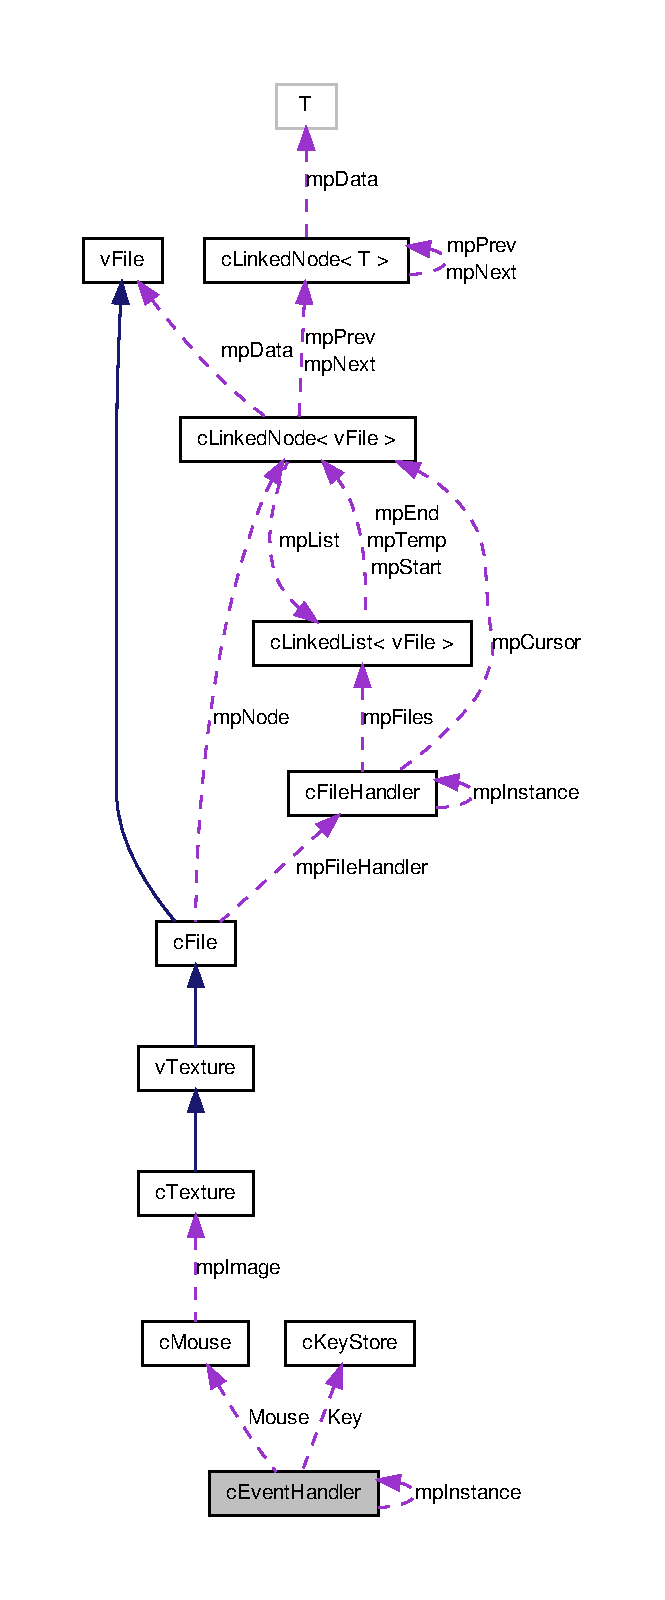
\includegraphics[width=257pt]{classc_event_handler__coll__graph}
\end{center}
\end{figure}
\subsection*{Static Public Member Functions}
\begin{DoxyCompactItemize}
\item 
\hypertarget{classc_event_handler_a8cf5519e1f3c5f6a6f79f9da75fb2750}{
static \hyperlink{classc_event_handler}{cEventHandler} $\ast$ \hyperlink{classc_event_handler_a8cf5519e1f3c5f6a6f79f9da75fb2750}{Instance} ()}
\label{classc_event_handler_a8cf5519e1f3c5f6a6f79f9da75fb2750}

\begin{DoxyCompactList}\small\item\em This will return a pointer to the current cEventhandler instance. If there is no instance it will create one. \end{DoxyCompactList}\end{DoxyCompactItemize}
\subsection*{Public Attributes}
\begin{DoxyCompactItemize}
\item 
\hypertarget{classc_event_handler_a53ba15cada383fb64c9918d8ce923585}{
\hyperlink{classc_key_store}{cKeyStore} \hyperlink{classc_event_handler_a53ba15cada383fb64c9918d8ce923585}{Key}}
\label{classc_event_handler_a53ba15cada383fb64c9918d8ce923585}

\begin{DoxyCompactList}\small\item\em This will store all the keyboard input data. see \_\-KEY. \end{DoxyCompactList}\item 
\hypertarget{classc_event_handler_a5d871cf2ddea710db2b4daed30cd1866}{
\hyperlink{classc_mouse}{cMouse} \hyperlink{classc_event_handler_a5d871cf2ddea710db2b4daed30cd1866}{MouseDevice}}
\label{classc_event_handler_a5d871cf2ddea710db2b4daed30cd1866}

\begin{DoxyCompactList}\small\item\em This will store the mouse input data. see \_\-MOUSE. \end{DoxyCompactList}\end{DoxyCompactItemize}


\subsection{Detailed Description}
This will handle events from the OS. Actually this will just store the Input data for the keyboard and mouse. It is easiest to access the input data using \_\-KEY and \_\-MOUSE. There can only be one \hyperlink{classc_event_handler}{cEventHandler}, created using \hyperlink{classc_event_handler_a8cf5519e1f3c5f6a6f79f9da75fb2750}{Instance()}. 
\hypertarget{class_c_exception}{
\section{CException Class Reference}
\label{class_c_exception}\index{CException@{CException}}
}
\subsection*{Public Member Functions}
\begin{DoxyCompactItemize}
\item 
\hyperlink{class_c_exception_a0a70072f86f6b47efd2fe15e1091a608}{CException} (const char $\ast$m)
\item 
\hyperlink{class_c_exception_aade9fea992258b659e40c3165a1fd223}{CException} (string \&m)
\end{DoxyCompactItemize}
\subsection*{Public Attributes}
\begin{DoxyCompactItemize}
\item 
string \hyperlink{class_c_exception_a89577adf63532606163fbce2a70bf012}{message}
\end{DoxyCompactItemize}


\subsection{Detailed Description}


Definition at line 8 of file CException.h.



\subsection{Constructor \& Destructor Documentation}
\hypertarget{class_c_exception_a0a70072f86f6b47efd2fe15e1091a608}{
\index{CException@{CException}!CException@{CException}}
\index{CException@{CException}!CException@{CException}}
\subsubsection[{CException}]{\setlength{\rightskip}{0pt plus 5cm}CException::CException (
\begin{DoxyParamCaption}
\item[{const char $\ast$}]{m}
\end{DoxyParamCaption}
)\hspace{0.3cm}{\ttfamily  \mbox{[}inline\mbox{]}}}}
\label{class_c_exception_a0a70072f86f6b47efd2fe15e1091a608}


Definition at line 11 of file CException.h.

\hypertarget{class_c_exception_aade9fea992258b659e40c3165a1fd223}{
\index{CException@{CException}!CException@{CException}}
\index{CException@{CException}!CException@{CException}}
\subsubsection[{CException}]{\setlength{\rightskip}{0pt plus 5cm}CException::CException (
\begin{DoxyParamCaption}
\item[{string \&}]{m}
\end{DoxyParamCaption}
)\hspace{0.3cm}{\ttfamily  \mbox{[}inline\mbox{]}}}}
\label{class_c_exception_aade9fea992258b659e40c3165a1fd223}


Definition at line 12 of file CException.h.



\subsection{Member Data Documentation}
\hypertarget{class_c_exception_a89577adf63532606163fbce2a70bf012}{
\index{CException@{CException}!message@{message}}
\index{message@{message}!CException@{CException}}
\subsubsection[{message}]{\setlength{\rightskip}{0pt plus 5cm}string {\bf CException::message}}}
\label{class_c_exception_a89577adf63532606163fbce2a70bf012}


Definition at line 10 of file CException.h.


\hypertarget{classc_face}{
\section{cFace Class Reference}
\label{classc_face}\index{cFace@{cFace}}
}


This class will store data about faces for a 3D Mesh. This can be used for Models, Collision Meshes or any other object using 3D Faces. Includes code for loading and saving the object types to and from IMF Files. Uses \hyperlink{classc_vertex}{cVertex} and \hyperlink{classc_plane}{cPlane} to store the data.  




Inheritance diagram for cFace:
\nopagebreak
\begin{figure}[H]
\begin{center}
\leavevmode
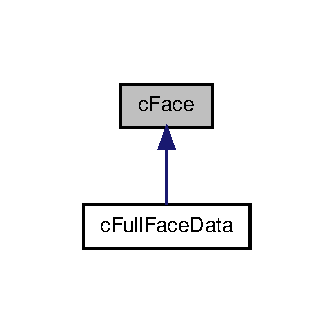
\includegraphics[width=160pt]{classc_face__inherit__graph}
\end{center}
\end{figure}


Collaboration diagram for cFace:
\nopagebreak
\begin{figure}[H]
\begin{center}
\leavevmode
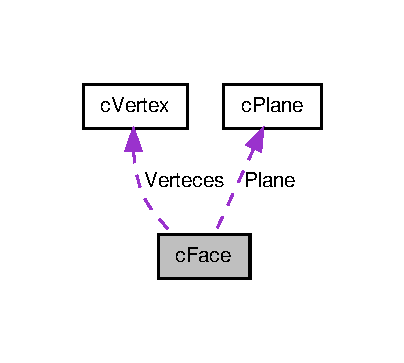
\includegraphics[width=194pt]{classc_face__coll__graph}
\end{center}
\end{figure}
\subsection*{Public Member Functions}
\begin{DoxyCompactItemize}
\item 
\hyperlink{classc_face}{cFace} \& \hyperlink{classc_face_aff51f522716a340fe0f0b3c55ab68bff}{operator=} (\hyperlink{classc_face}{cFace} \&lpOther)
\item 
uint32 \hyperlink{classc_face_ac2da0ca5e4269e12016b74c6443cde32}{FileSize} ()
\item 
void \hyperlink{classc_face_a1b1ff8e5ec5f30b1140e7f1e71086ed5}{OutputIMFFace} (ofstream \&FileStream)
\item 
void \hyperlink{classc_face_a8a39f8e4a8bf051dc67c7f55a88d636b}{LoadIMFFace} (ifstream \&FileStream)
\end{DoxyCompactItemize}
\subsection*{Public Attributes}
\begin{DoxyCompactItemize}
\item 
\hyperlink{classc_vertex}{cVertex} \hyperlink{classc_face_ae08ccc2952b022dce6848628649d61c8}{Verteces} \mbox{[}3\mbox{]}
\item 
\hyperlink{classc_plane}{cPlane} \hyperlink{classc_face_aa61d6dca6df8211a1a816edbf303bd27}{Plane}
\end{DoxyCompactItemize}


\subsection{Detailed Description}
This class will store data about faces for a 3D Mesh. This can be used for Models, Collision Meshes or any other object using 3D Faces. Includes code for loading and saving the object types to and from IMF Files. Uses \hyperlink{classc_vertex}{cVertex} and \hyperlink{classc_plane}{cPlane} to store the data. 

Definition at line 7 of file WTcFace.h.



\subsection{Member Function Documentation}
\hypertarget{classc_face_ac2da0ca5e4269e12016b74c6443cde32}{
\index{cFace@{cFace}!FileSize@{FileSize}}
\index{FileSize@{FileSize}!cFace@{cFace}}
\subsubsection[{FileSize}]{\setlength{\rightskip}{0pt plus 5cm}uint32 cFace::FileSize (
\begin{DoxyParamCaption}
{}
\end{DoxyParamCaption}
)}}
\label{classc_face_ac2da0ca5e4269e12016b74c6443cde32}


Reimplemented in \hyperlink{classc_full_face_data_a53a99ced9de4ecdede38b2e8d63458e9}{cFullFaceData}.



Definition at line 12 of file WTcFace.cpp.

\hypertarget{classc_face_a8a39f8e4a8bf051dc67c7f55a88d636b}{
\index{cFace@{cFace}!LoadIMFFace@{LoadIMFFace}}
\index{LoadIMFFace@{LoadIMFFace}!cFace@{cFace}}
\subsubsection[{LoadIMFFace}]{\setlength{\rightskip}{0pt plus 5cm}void cFace::LoadIMFFace (
\begin{DoxyParamCaption}
\item[{ifstream \&}]{FileStream}
\end{DoxyParamCaption}
)}}
\label{classc_face_a8a39f8e4a8bf051dc67c7f55a88d636b}


Definition at line 33 of file WTcFace.cpp.

\hypertarget{classc_face_aff51f522716a340fe0f0b3c55ab68bff}{
\index{cFace@{cFace}!operator=@{operator=}}
\index{operator=@{operator=}!cFace@{cFace}}
\subsubsection[{operator=}]{\setlength{\rightskip}{0pt plus 5cm}{\bf cFace} \& cFace::operator= (
\begin{DoxyParamCaption}
\item[{{\bf cFace} \&}]{lpOther}
\end{DoxyParamCaption}
)}}
\label{classc_face_aff51f522716a340fe0f0b3c55ab68bff}


Definition at line 3 of file WTcFace.cpp.

\hypertarget{classc_face_a1b1ff8e5ec5f30b1140e7f1e71086ed5}{
\index{cFace@{cFace}!OutputIMFFace@{OutputIMFFace}}
\index{OutputIMFFace@{OutputIMFFace}!cFace@{cFace}}
\subsubsection[{OutputIMFFace}]{\setlength{\rightskip}{0pt plus 5cm}void cFace::OutputIMFFace (
\begin{DoxyParamCaption}
\item[{ofstream \&}]{FileStream}
\end{DoxyParamCaption}
)}}
\label{classc_face_a1b1ff8e5ec5f30b1140e7f1e71086ed5}


Definition at line 24 of file WTcFace.cpp.



\subsection{Member Data Documentation}
\hypertarget{classc_face_aa61d6dca6df8211a1a816edbf303bd27}{
\index{cFace@{cFace}!Plane@{Plane}}
\index{Plane@{Plane}!cFace@{cFace}}
\subsubsection[{Plane}]{\setlength{\rightskip}{0pt plus 5cm}{\bf cPlane} {\bf cFace::Plane}}}
\label{classc_face_aa61d6dca6df8211a1a816edbf303bd27}


Definition at line 12 of file WTcFace.h.

\hypertarget{classc_face_ae08ccc2952b022dce6848628649d61c8}{
\index{cFace@{cFace}!Verteces@{Verteces}}
\index{Verteces@{Verteces}!cFace@{cFace}}
\subsubsection[{Verteces}]{\setlength{\rightskip}{0pt plus 5cm}{\bf cVertex} {\bf cFace::Verteces}\mbox{[}3\mbox{]}}}
\label{classc_face_ae08ccc2952b022dce6848628649d61c8}


Definition at line 11 of file WTcFace.h.


\hypertarget{classc_file}{
\section{cFile Class Reference}
\label{classc_file}\index{cFile@{cFile}}
}


This is the base code for files to be loaded from a hdd. Any file object loaded from a hddvshould inherit this class. It is best used for media files. This code will automatically add newly loaded files to \hyperlink{classc_file_handler}{cFileHandler}. The files can be loaded using the filename or if loaded from an IMF file using the reference for each file.  




Collaboration diagram for cFile:\nopagebreak
\begin{figure}[H]
\begin{center}
\leavevmode
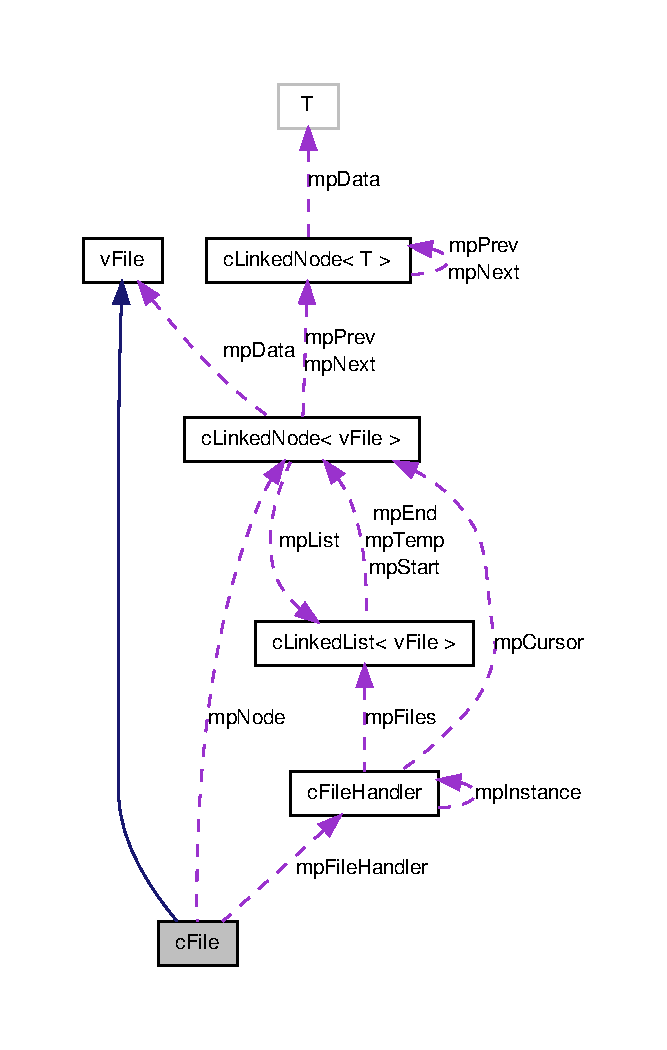
\includegraphics[width=320pt]{classc_file__coll__graph}
\end{center}
\end{figure}
\subsection*{Public Member Functions}
\begin{DoxyCompactItemize}
\item 
\hypertarget{classc_file_a5bb81f36e954af61b581e3c1fd06e0de}{
\hyperlink{classc_file_a5bb81f36e954af61b581e3c1fd06e0de}{cFile} ()}
\label{classc_file_a5bb81f36e954af61b581e3c1fd06e0de}

\begin{DoxyCompactList}\small\item\em This constructor will automatically load the file from memory and add it to the list in cFilehandler. \end{DoxyCompactList}\item 
\hypertarget{classc_file_a7224559b2485e53608bd6ba9e21d1122}{
char $\ast$ \hyperlink{classc_file_a7224559b2485e53608bd6ba9e21d1122}{FileName} ()}
\label{classc_file_a7224559b2485e53608bd6ba9e21d1122}

\begin{DoxyCompactList}\small\item\em This will return the files filename. \end{DoxyCompactList}\item 
\hypertarget{classc_file_aa5891f6208183a26e7fde7d8dee62ffc}{
void \hyperlink{classc_file_aa5891f6208183a26e7fde7d8dee62ffc}{Load} ()}
\label{classc_file_aa5891f6208183a26e7fde7d8dee62ffc}

\begin{DoxyCompactList}\small\item\em This is the function that will actually load the file from a hdd. \end{DoxyCompactList}\item 
\hypertarget{classc_file_ab2e74ccc027ccb92ea577cd7bb9b5f5c}{
void \hyperlink{classc_file_ab2e74ccc027ccb92ea577cd7bb9b5f5c}{Delete} ()}
\label{classc_file_ab2e74ccc027ccb92ea577cd7bb9b5f5c}

\begin{DoxyCompactList}\small\item\em This will delete the file from memory. \end{DoxyCompactList}\end{DoxyCompactItemize}
\subsection*{Public Attributes}
\begin{DoxyCompactItemize}
\item 
\hypertarget{classc_file_aed51bea596b50e6c8a03dd1593298681}{
\hyperlink{classc_linked_node}{cLinkedNode}$<$ \hyperlink{classv_file}{vFile} $>$ $\ast$ \hyperlink{classc_file_aed51bea596b50e6c8a03dd1593298681}{mpNode}}
\label{classc_file_aed51bea596b50e6c8a03dd1593298681}

\begin{DoxyCompactList}\small\item\em This is a pointer to the \hyperlink{classc_linked_node}{cLinkedNode} which owns this file. \end{DoxyCompactList}\item 
\hypertarget{classc_file_a5e3add41cacddcc489ca9aa185e3b066}{
char \hyperlink{classc_file_a5e3add41cacddcc489ca9aa185e3b066}{mpFileName} \mbox{[}64\mbox{]}}
\label{classc_file_a5e3add41cacddcc489ca9aa185e3b066}

\begin{DoxyCompactList}\small\item\em This will store the files filename. \end{DoxyCompactList}\end{DoxyCompactItemize}
\subsection*{Protected Attributes}
\begin{DoxyCompactItemize}
\item 
\hypertarget{classc_file_ae54eca20c29d2fcd5649aac33d1dba9a}{
\hyperlink{classc_file_handler}{cFileHandler} $\ast$ \hyperlink{classc_file_ae54eca20c29d2fcd5649aac33d1dba9a}{mpFileHandler}}
\label{classc_file_ae54eca20c29d2fcd5649aac33d1dba9a}

\begin{DoxyCompactList}\small\item\em This is a pointer to the \hyperlink{classc_file_handler}{cFileHandler} which owns this file. \end{DoxyCompactList}\end{DoxyCompactItemize}
\subsection*{Friends}
\begin{DoxyCompactItemize}
\item 
\hypertarget{classc_file_a70d0eacda2243b6345feb400aef70378}{
class \hyperlink{classc_file_a70d0eacda2243b6345feb400aef70378}{cFileHandler}}
\label{classc_file_a70d0eacda2243b6345feb400aef70378}

\end{DoxyCompactItemize}


\subsection{Detailed Description}
This is the base code for files to be loaded from a hdd. Any file object loaded from a hddvshould inherit this class. It is best used for media files. This code will automatically add newly loaded files to \hyperlink{classc_file_handler}{cFileHandler}. The files can be loaded using the filename or if loaded from an IMF file using the reference for each file. 
\hypertarget{classc_file_handler}{
\section{cFileHandler Class Reference}
\label{classc_file_handler}\index{cFileHandler@{cFileHandler}}
}


This is the handler for the file system. This handles all files loaded from a hdd. It will give allow processes to use files loaded else where, using either the filenames or if loaded from an IMF a file reference. The files are stored in the list mpFiles.  




Collaboration diagram for cFileHandler:
\nopagebreak
\begin{figure}[H]
\begin{center}
\leavevmode
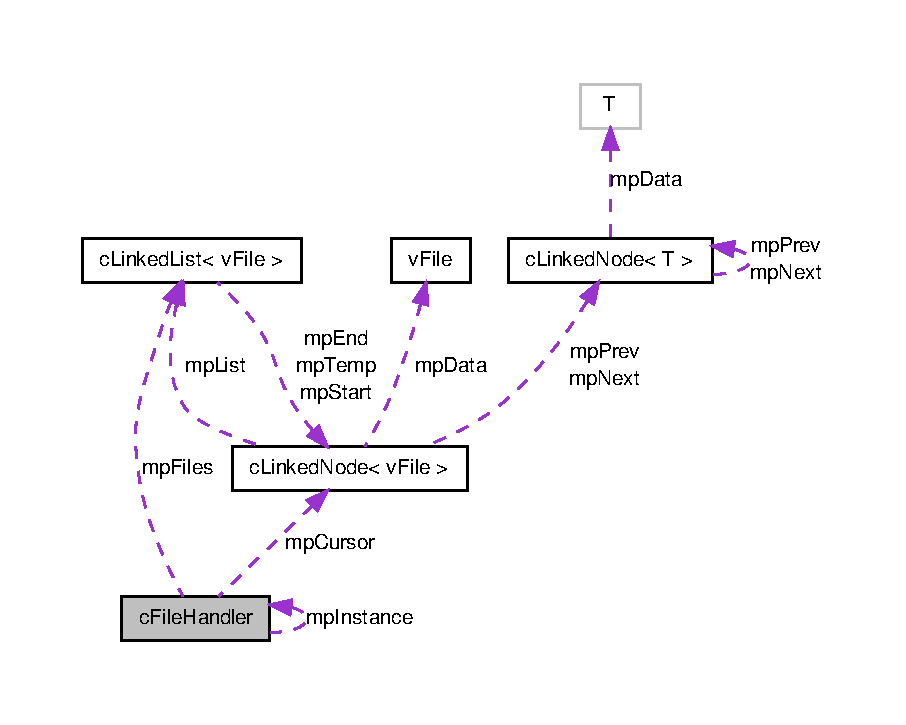
\includegraphics[width=400pt]{classc_file_handler__coll__graph}
\end{center}
\end{figure}
\subsection*{Public Member Functions}
\begin{DoxyCompactItemize}
\item 
\hyperlink{classc_file_handler_a88dd9099f9332245a2f2fc8a3eb8abc5}{$\sim$cFileHandler} ()
\item 
void \hyperlink{classc_file_handler_a87ff1f0cc36ef46514f77826eaf04453}{Reload} ()
\begin{DoxyCompactList}\small\item\em This will reload all the files from a hdd into memory. (Note this is not currently complete). \item\end{DoxyCompactList}\item 
void \hyperlink{classc_file_handler_a610399fa5d6bdb45de1d3cdc4dcb4c3c}{Unload} ()
\begin{DoxyCompactList}\small\item\em This will remove all the files from memory. (Note this is not currently complete). \item\end{DoxyCompactList}\item 
void $\ast$ \hyperlink{classc_file_handler_a3d2432f40a2d8f2fed223b6ad508b7df}{File} (const char $\ast$lpFilename)
\begin{DoxyCompactList}\small\item\em This will return a pointer to a file with the filename or file refernce lpFilename. \item\end{DoxyCompactList}\item 
\hyperlink{classc_linked_node}{cLinkedNode}$<$ \hyperlink{classv_file}{vFile} $>$ $\ast$ \hyperlink{classc_file_handler_a30b1285eaca092f8417c3f1750f60559}{Add} (\hyperlink{classv_file}{vFile} $\ast$lpNew)
\begin{DoxyCompactList}\small\item\em This will add the file pointed to by lpNew to the current file list mpFile. \item\end{DoxyCompactList}\item 
void \hyperlink{classc_file_handler_a2701aa77518747a401b51e0c38ba1cd1}{Delete} (\hyperlink{classc_linked_node}{cLinkedNode}$<$ \hyperlink{classv_file}{vFile} $>$ $\ast$lpNode)
\begin{DoxyCompactList}\small\item\em This will delete the file owned by lpNode from the file list mpFile. \item\end{DoxyCompactList}\end{DoxyCompactItemize}
\subsection*{Static Public Member Functions}
\begin{DoxyCompactItemize}
\item 
static \hyperlink{classc_file_handler}{cFileHandler} $\ast$ \hyperlink{classc_file_handler_a99495051a1a41a763113aca5292023b9}{Instance} ()
\begin{DoxyCompactList}\small\item\em This will return a pointer to the current \hyperlink{classc_file_handler}{cFileHandler}. If there is no current instance it will create one and return the pointer. \item\end{DoxyCompactList}\end{DoxyCompactItemize}


\subsection{Detailed Description}
This is the handler for the file system. This handles all files loaded from a hdd. It will give allow processes to use files loaded else where, using either the filenames or if loaded from an IMF a file reference. The files are stored in the list mpFiles. 

Definition at line 10 of file WTcFileHandler.h.



\subsection{Constructor \& Destructor Documentation}
\hypertarget{classc_file_handler_a88dd9099f9332245a2f2fc8a3eb8abc5}{
\index{cFileHandler@{cFileHandler}!$\sim$cFileHandler@{$\sim$cFileHandler}}
\index{$\sim$cFileHandler@{$\sim$cFileHandler}!cFileHandler@{cFileHandler}}
\subsubsection[{$\sim$cFileHandler}]{\setlength{\rightskip}{0pt plus 5cm}cFileHandler::$\sim$cFileHandler (
\begin{DoxyParamCaption}
{}
\end{DoxyParamCaption}
)}}
\label{classc_file_handler_a88dd9099f9332245a2f2fc8a3eb8abc5}


Definition at line 24 of file WTcFileHandler.cpp.



\subsection{Member Function Documentation}
\hypertarget{classc_file_handler_a30b1285eaca092f8417c3f1750f60559}{
\index{cFileHandler@{cFileHandler}!Add@{Add}}
\index{Add@{Add}!cFileHandler@{cFileHandler}}
\subsubsection[{Add}]{\setlength{\rightskip}{0pt plus 5cm}{\bf cLinkedNode}$<$ {\bf vFile} $>$ $\ast$ cFileHandler::Add (
\begin{DoxyParamCaption}
\item[{{\bf vFile} $\ast$}]{lpNew}
\end{DoxyParamCaption}
)}}
\label{classc_file_handler_a30b1285eaca092f8417c3f1750f60559}


This will add the file pointed to by lpNew to the current file list mpFile. 



Definition at line 43 of file WTcFileHandler.cpp.

\hypertarget{classc_file_handler_a2701aa77518747a401b51e0c38ba1cd1}{
\index{cFileHandler@{cFileHandler}!Delete@{Delete}}
\index{Delete@{Delete}!cFileHandler@{cFileHandler}}
\subsubsection[{Delete}]{\setlength{\rightskip}{0pt plus 5cm}void cFileHandler::Delete (
\begin{DoxyParamCaption}
\item[{{\bf cLinkedNode}$<$ {\bf vFile} $>$ $\ast$}]{lpNode}
\end{DoxyParamCaption}
)}}
\label{classc_file_handler_a2701aa77518747a401b51e0c38ba1cd1}


This will delete the file owned by lpNode from the file list mpFile. 



Definition at line 52 of file WTcFileHandler.cpp.

\hypertarget{classc_file_handler_a3d2432f40a2d8f2fed223b6ad508b7df}{
\index{cFileHandler@{cFileHandler}!File@{File}}
\index{File@{File}!cFileHandler@{cFileHandler}}
\subsubsection[{File}]{\setlength{\rightskip}{0pt plus 5cm}void $\ast$ cFileHandler::File (
\begin{DoxyParamCaption}
\item[{const char $\ast$}]{lpFilename}
\end{DoxyParamCaption}
)}}
\label{classc_file_handler_a3d2432f40a2d8f2fed223b6ad508b7df}


This will return a pointer to a file with the filename or file refernce lpFilename. 



Definition at line 9 of file WTcFileHandler.cpp.

\hypertarget{classc_file_handler_a99495051a1a41a763113aca5292023b9}{
\index{cFileHandler@{cFileHandler}!Instance@{Instance}}
\index{Instance@{Instance}!cFileHandler@{cFileHandler}}
\subsubsection[{Instance}]{\setlength{\rightskip}{0pt plus 5cm}{\bf cFileHandler} $\ast$ cFileHandler::Instance (
\begin{DoxyParamCaption}
{}
\end{DoxyParamCaption}
)\hspace{0.3cm}{\ttfamily  \mbox{[}static\mbox{]}}}}
\label{classc_file_handler_a99495051a1a41a763113aca5292023b9}


This will return a pointer to the current \hyperlink{classc_file_handler}{cFileHandler}. If there is no current instance it will create one and return the pointer. 



Definition at line 33 of file WTcFileHandler.cpp.

\hypertarget{classc_file_handler_a87ff1f0cc36ef46514f77826eaf04453}{
\index{cFileHandler@{cFileHandler}!Reload@{Reload}}
\index{Reload@{Reload}!cFileHandler@{cFileHandler}}
\subsubsection[{Reload}]{\setlength{\rightskip}{0pt plus 5cm}void cFileHandler::Reload (
\begin{DoxyParamCaption}
{}
\end{DoxyParamCaption}
)}}
\label{classc_file_handler_a87ff1f0cc36ef46514f77826eaf04453}


This will reload all the files from a hdd into memory. (Note this is not currently complete). 



Definition at line 39 of file WTcFileHandler.cpp.

\hypertarget{classc_file_handler_a610399fa5d6bdb45de1d3cdc4dcb4c3c}{
\index{cFileHandler@{cFileHandler}!Unload@{Unload}}
\index{Unload@{Unload}!cFileHandler@{cFileHandler}}
\subsubsection[{Unload}]{\setlength{\rightskip}{0pt plus 5cm}void cFileHandler::Unload (
\begin{DoxyParamCaption}
{}
\end{DoxyParamCaption}
)}}
\label{classc_file_handler_a610399fa5d6bdb45de1d3cdc4dcb4c3c}


This will remove all the files from memory. (Note this is not currently complete). 



Definition at line 41 of file WTcFileHandler.cpp.


\hypertarget{classc_fog}{
\section{cFog Class Reference}
\label{classc_fog}\index{cFog@{cFog}}
}


This class will create and control an OpenGL scenes fog effect.  


\subsection*{Public Member Functions}
\begin{DoxyCompactItemize}
\item 
\hyperlink{classc_fog_a8d87f9ec7b741a27236b89f134f46104}{cFog} ()
\begin{DoxyCompactList}\small\item\em Creates a clear fog effect. \item\end{DoxyCompactList}\item 
\hyperlink{classc_fog_a546279d0cae73376c9b254b727c32a50}{cFog} (float lfStart, float lfEnd)
\begin{DoxyCompactList}\small\item\em Creates a new fog object between distance lfStart and lfEnd. \item\end{DoxyCompactList}\item 
void \hyperlink{classc_fog_a6df07427d17c1ebae3d9fda3a8c35071}{SetColor} (float lfRed, float lfGreen, float lfBlue, float lfAlpha)
\begin{DoxyCompactList}\small\item\em Will set the RGBA color of the fog. \item\end{DoxyCompactList}\item 
void \hyperlink{classc_fog_a295ed5f6c4d99814a14740a4527d090f}{SetMode} (char ltMode)
\begin{DoxyCompactList}\small\item\em Will set the fog equation the fog effect will use. (GL\_\-EXP, GL\_\-EXP2, GL\_\-LINEAR) \item\end{DoxyCompactList}\item 
void \hyperlink{classc_fog_a0de4a3634f298570163182df50813e90}{SetDensity} (float lfDensity)
\begin{DoxyCompactList}\small\item\em Will set the effect the fog has on the screen colors. 1.0f is Opaque, 0.0f is completely transparent. \item\end{DoxyCompactList}\item 
void \hyperlink{classc_fog_a94f49aea8c21e90755fb365c1aa6d443}{SetRange} (float lfStart, float lfEnd)
\begin{DoxyCompactList}\small\item\em Will set the near and far distances, from the camera, of the fog effect. \item\end{DoxyCompactList}\item 
bool \hyperlink{classc_fog_a00959c3267cb56abf20e0e9bf0cec329}{On} ()
\begin{DoxyCompactList}\small\item\em Will return whether the fog effect is on or off. \item\end{DoxyCompactList}\item 
void \hyperlink{classc_fog_a948265685f32d2e08a7e67632419f73b}{SetOn} ()
\begin{DoxyCompactList}\small\item\em Will set the fog effect on. \item\end{DoxyCompactList}\item 
void \hyperlink{classc_fog_a784bb1ece1382e294dfce8b6bb52d033}{SetOff} ()
\begin{DoxyCompactList}\small\item\em Will set the fog effect off. \item\end{DoxyCompactList}\end{DoxyCompactItemize}


\subsection{Detailed Description}
This class will create and control an OpenGL scenes fog effect. 

Definition at line 7 of file WTcFog.h.



\subsection{Constructor \& Destructor Documentation}
\hypertarget{classc_fog_a8d87f9ec7b741a27236b89f134f46104}{
\index{cFog@{cFog}!cFog@{cFog}}
\index{cFog@{cFog}!cFog@{cFog}}
\subsubsection[{cFog}]{\setlength{\rightskip}{0pt plus 5cm}cFog::cFog (
\begin{DoxyParamCaption}
{}
\end{DoxyParamCaption}
)}}
\label{classc_fog_a8d87f9ec7b741a27236b89f134f46104}


Creates a clear fog effect. 



Definition at line 3 of file WTcFog.cpp.

\hypertarget{classc_fog_a546279d0cae73376c9b254b727c32a50}{
\index{cFog@{cFog}!cFog@{cFog}}
\index{cFog@{cFog}!cFog@{cFog}}
\subsubsection[{cFog}]{\setlength{\rightskip}{0pt plus 5cm}cFog::cFog (
\begin{DoxyParamCaption}
\item[{float}]{lfStart, }
\item[{float}]{lfEnd}
\end{DoxyParamCaption}
)}}
\label{classc_fog_a546279d0cae73376c9b254b727c32a50}


Creates a new fog object between distance lfStart and lfEnd. 



Definition at line 18 of file WTcFog.cpp.



\subsection{Member Function Documentation}
\hypertarget{classc_fog_a00959c3267cb56abf20e0e9bf0cec329}{
\index{cFog@{cFog}!On@{On}}
\index{On@{On}!cFog@{cFog}}
\subsubsection[{On}]{\setlength{\rightskip}{0pt plus 5cm}bool cFog::On (
\begin{DoxyParamCaption}
{}
\end{DoxyParamCaption}
)}}
\label{classc_fog_a00959c3267cb56abf20e0e9bf0cec329}


Will return whether the fog effect is on or off. 



Definition at line 77 of file WTcFog.cpp.

\hypertarget{classc_fog_a6df07427d17c1ebae3d9fda3a8c35071}{
\index{cFog@{cFog}!SetColor@{SetColor}}
\index{SetColor@{SetColor}!cFog@{cFog}}
\subsubsection[{SetColor}]{\setlength{\rightskip}{0pt plus 5cm}void cFog::SetColor (
\begin{DoxyParamCaption}
\item[{float}]{lfRed, }
\item[{float}]{lfGreen, }
\item[{float}]{lfBlue, }
\item[{float}]{lfAlpha}
\end{DoxyParamCaption}
)}}
\label{classc_fog_a6df07427d17c1ebae3d9fda3a8c35071}


Will set the RGBA color of the fog. 



Definition at line 50 of file WTcFog.cpp.

\hypertarget{classc_fog_a0de4a3634f298570163182df50813e90}{
\index{cFog@{cFog}!SetDensity@{SetDensity}}
\index{SetDensity@{SetDensity}!cFog@{cFog}}
\subsubsection[{SetDensity}]{\setlength{\rightskip}{0pt plus 5cm}void cFog::SetDensity (
\begin{DoxyParamCaption}
\item[{float}]{lfDensity}
\end{DoxyParamCaption}
)}}
\label{classc_fog_a0de4a3634f298570163182df50813e90}


Will set the effect the fog has on the screen colors. 1.0f is Opaque, 0.0f is completely transparent. 



Definition at line 64 of file WTcFog.cpp.

\hypertarget{classc_fog_a295ed5f6c4d99814a14740a4527d090f}{
\index{cFog@{cFog}!SetMode@{SetMode}}
\index{SetMode@{SetMode}!cFog@{cFog}}
\subsubsection[{SetMode}]{\setlength{\rightskip}{0pt plus 5cm}void cFog::SetMode (
\begin{DoxyParamCaption}
\item[{char}]{ltMode}
\end{DoxyParamCaption}
)}}
\label{classc_fog_a295ed5f6c4d99814a14740a4527d090f}


Will set the fog equation the fog effect will use. (GL\_\-EXP, GL\_\-EXP2, GL\_\-LINEAR) 



Definition at line 58 of file WTcFog.cpp.

\hypertarget{classc_fog_a784bb1ece1382e294dfce8b6bb52d033}{
\index{cFog@{cFog}!SetOff@{SetOff}}
\index{SetOff@{SetOff}!cFog@{cFog}}
\subsubsection[{SetOff}]{\setlength{\rightskip}{0pt plus 5cm}void cFog::SetOff (
\begin{DoxyParamCaption}
{}
\end{DoxyParamCaption}
)}}
\label{classc_fog_a784bb1ece1382e294dfce8b6bb52d033}


Will set the fog effect off. 



Definition at line 45 of file WTcFog.cpp.

\hypertarget{classc_fog_a948265685f32d2e08a7e67632419f73b}{
\index{cFog@{cFog}!SetOn@{SetOn}}
\index{SetOn@{SetOn}!cFog@{cFog}}
\subsubsection[{SetOn}]{\setlength{\rightskip}{0pt plus 5cm}void cFog::SetOn (
\begin{DoxyParamCaption}
{}
\end{DoxyParamCaption}
)}}
\label{classc_fog_a948265685f32d2e08a7e67632419f73b}


Will set the fog effect on. 



Definition at line 34 of file WTcFog.cpp.

\hypertarget{classc_fog_a94f49aea8c21e90755fb365c1aa6d443}{
\index{cFog@{cFog}!SetRange@{SetRange}}
\index{SetRange@{SetRange}!cFog@{cFog}}
\subsubsection[{SetRange}]{\setlength{\rightskip}{0pt plus 5cm}void cFog::SetRange (
\begin{DoxyParamCaption}
\item[{float}]{lfStart, }
\item[{float}]{lfEnd}
\end{DoxyParamCaption}
)}}
\label{classc_fog_a94f49aea8c21e90755fb365c1aa6d443}


Will set the near and far distances, from the camera, of the fog effect. 



Definition at line 71 of file WTcFog.cpp.


\hypertarget{classc_font}{
\section{cFont Class Reference}
\label{classc_font}\index{cFont@{cFont}}
}


This class will store the data for a Font ready to be used for rendering \hyperlink{classc_text}{cText}. This should come from an IMF file and be composed of an image of 93 character images stacked vertically. This is a file class and should be handled entirely by the engine.  




Collaboration diagram for cFont:\nopagebreak
\begin{figure}[H]
\begin{center}
\leavevmode
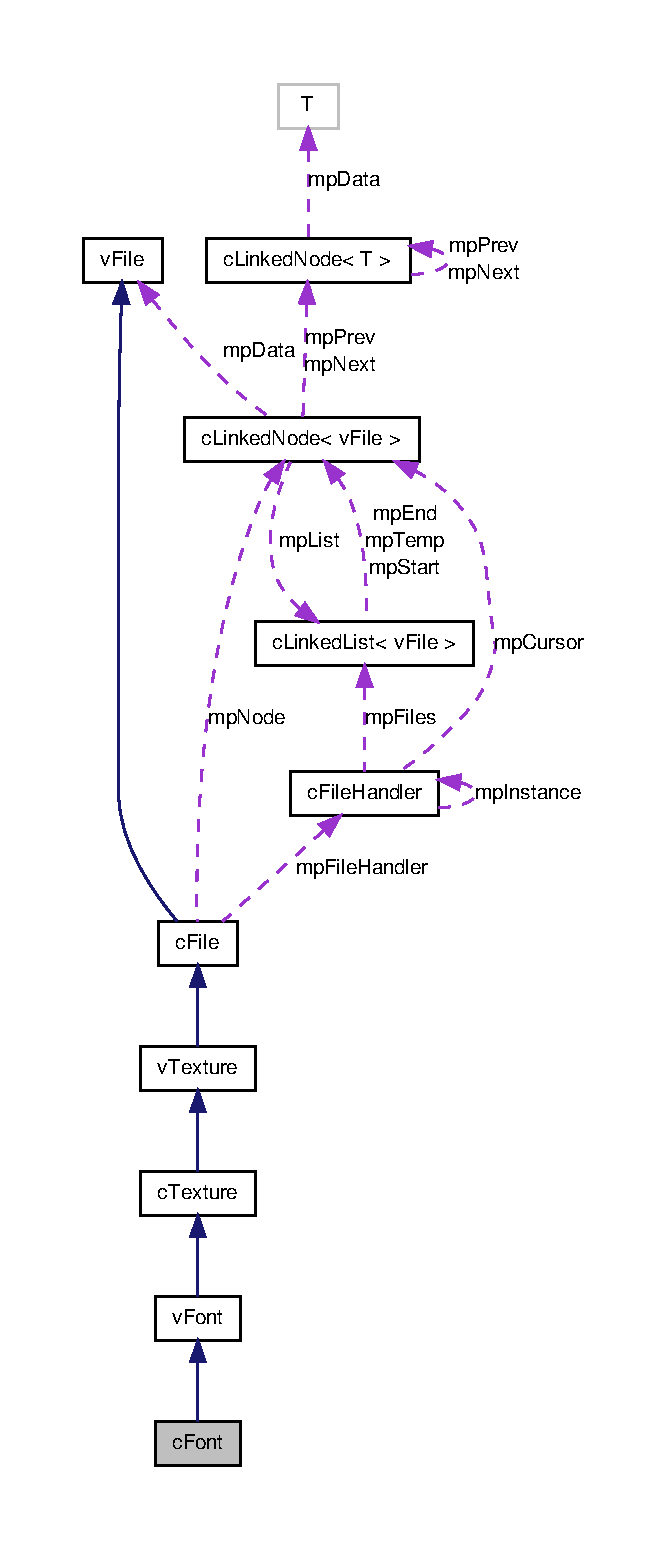
\includegraphics[width=320pt]{classc_font__coll__graph}
\end{center}
\end{figure}
\subsection*{Public Member Functions}
\begin{DoxyCompactItemize}
\item 
\hypertarget{classc_font_a3fa379c0126af4edd8c4f7bb39507a13}{
uint32 \hyperlink{classc_font_a3fa379c0126af4edd8c4f7bb39507a13}{Height} ()}
\label{classc_font_a3fa379c0126af4edd8c4f7bb39507a13}

\begin{DoxyCompactList}\small\item\em Returns the \hyperlink{classc_texture}{cTexture} Height. \end{DoxyCompactList}\end{DoxyCompactItemize}


\subsection{Detailed Description}
This class will store the data for a Font ready to be used for rendering \hyperlink{classc_text}{cText}. This should come from an IMF file and be composed of an image of 93 character images stacked vertically. This is a file class and should be handled entirely by the engine. 
\hypertarget{classc_frame_rate}{
\section{cFrameRate Class Reference}
\label{classc_frame_rate}\index{cFrameRate@{cFrameRate}}
}


This class will store data for controlling the Frame Rate. There are several settings that can be adjusted:\par
 Processes Per Frame:\par
 \par
 Frames Per Second:\par
 \par
 Frame Time and Process Time:\par
 These are the amount of time that passes every Frame and Process Cycle measured in seconds. Multiplying any distances moved by this will convert them into distance per second. This allows the user to change the running frame rate without affecting the speed the user experiences. If the Frame rate and Process Rate are not going to be changed this can be ignored.  




Collaboration diagram for cFrameRate:
\nopagebreak
\begin{figure}[H]
\begin{center}
\leavevmode
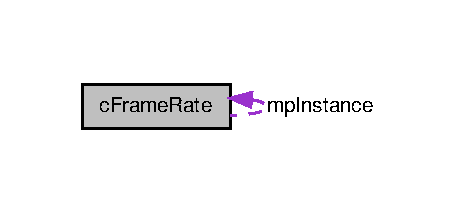
\includegraphics[width=220pt]{classc_frame_rate__coll__graph}
\end{center}
\end{figure}
\subsection*{Public Member Functions}
\begin{DoxyCompactItemize}
\item 
void \hyperlink{classc_frame_rate_a11d2578dfcb6eb2fea0bb331b7188dfe}{SetFrameRate} (uint8 lfFramesPerSecond)
\begin{DoxyCompactList}\small\item\em This is the number of Frames that will be rendered each second. This results in smooth consistent timings for every Process Cycle and Rendered Frame. This is best set to 60 / 70 though in extreme cases it can be set to 30. Rendering is very compoutationally expensive, so should be maintained at the lowest rate to produce a smooth visual image. \item\end{DoxyCompactList}\item 
void \hyperlink{classc_frame_rate_afb2bce05079fe1bc1e7b3ac3295fd692}{SetProcessesPerFrame} (uint8 liPPS)
\begin{DoxyCompactList}\small\item\em This is the number of times the Process cycle will be run for every rendered frame. Rendering is very slow and CPU intensive compared to the Procesing cycle. The Human eye cannot differentiate between very fast rendering rates, but increased numbers of processing cycles will increase accuracy of collisions and make events smoother. \item\end{DoxyCompactList}\item 
float \hyperlink{classc_frame_rate_a6af788062fd7f1cff658e19ca790219c}{FrameTime} ()
\begin{DoxyCompactList}\small\item\em this will return the amount of time that passes for every rendered frame. \item\end{DoxyCompactList}\item 
float \hyperlink{classc_frame_rate_ac314f1e240949dc74bd51730748ce1b2}{ProcessTime} ()
\begin{DoxyCompactList}\small\item\em This is the amount of time that passes every Process Cycle measured in seconds. Multiplying any distances moved by this will convert them into distance per second. This allows the user to change the running frame rate without affecting the speed the user experiences. If the Frame rate and Process Rate are not going to be changed this can be ignored. \item\end{DoxyCompactList}\item 
uint8 \hyperlink{classc_frame_rate_ab450d4c204172469695433474227bd19}{FramesPerSecond} ()
\begin{DoxyCompactList}\small\item\em This will return the current set number of Frames per Second. \item\end{DoxyCompactList}\item 
uint8 \hyperlink{classc_frame_rate_ab1b0bc7a9801cbea5d8036203a0a9ee4}{ProcessesPerFrame} ()
\begin{DoxyCompactList}\small\item\em this will return the current set number of Process Cycles per Rendered Frame. \item\end{DoxyCompactList}\end{DoxyCompactItemize}
\subsection*{Static Public Member Functions}
\begin{DoxyCompactItemize}
\item 
static \hyperlink{classc_frame_rate}{cFrameRate} $\ast$ \hyperlink{classc_frame_rate_a843b42d98bb70a1bc566a367b47d7fc3}{Instance} ()
\begin{DoxyCompactList}\small\item\em This will return a pointer to the current \hyperlink{classc_frame_rate}{cFrameRate} Object. \item\end{DoxyCompactList}\end{DoxyCompactItemize}


\subsection{Detailed Description}
This class will store data for controlling the Frame Rate. There are several settings that can be adjusted:\par
 Processes Per Frame:\par
 \par
 Frames Per Second:\par
 \par
 Frame Time and Process Time:\par
 These are the amount of time that passes every Frame and Process Cycle measured in seconds. Multiplying any distances moved by this will convert them into distance per second. This allows the user to change the running frame rate without affecting the speed the user experiences. If the Frame rate and Process Rate are not going to be changed this can be ignored. 

Definition at line 13 of file WTcFrameRate.h.



\subsection{Member Function Documentation}
\hypertarget{classc_frame_rate_ab450d4c204172469695433474227bd19}{
\index{cFrameRate@{cFrameRate}!FramesPerSecond@{FramesPerSecond}}
\index{FramesPerSecond@{FramesPerSecond}!cFrameRate@{cFrameRate}}
\subsubsection[{FramesPerSecond}]{\setlength{\rightskip}{0pt plus 5cm}uint8 cFrameRate::FramesPerSecond (
\begin{DoxyParamCaption}
{}
\end{DoxyParamCaption}
)}}
\label{classc_frame_rate_ab450d4c204172469695433474227bd19}


This will return the current set number of Frames per Second. 



Definition at line 23 of file WTcFrameRate.cpp.

\hypertarget{classc_frame_rate_a6af788062fd7f1cff658e19ca790219c}{
\index{cFrameRate@{cFrameRate}!FrameTime@{FrameTime}}
\index{FrameTime@{FrameTime}!cFrameRate@{cFrameRate}}
\subsubsection[{FrameTime}]{\setlength{\rightskip}{0pt plus 5cm}float cFrameRate::FrameTime (
\begin{DoxyParamCaption}
{}
\end{DoxyParamCaption}
)}}
\label{classc_frame_rate_a6af788062fd7f1cff658e19ca790219c}


this will return the amount of time that passes for every rendered frame. 



Definition at line 21 of file WTcFrameRate.cpp.

\hypertarget{classc_frame_rate_a843b42d98bb70a1bc566a367b47d7fc3}{
\index{cFrameRate@{cFrameRate}!Instance@{Instance}}
\index{Instance@{Instance}!cFrameRate@{cFrameRate}}
\subsubsection[{Instance}]{\setlength{\rightskip}{0pt plus 5cm}{\bf cFrameRate} $\ast$ cFrameRate::Instance (
\begin{DoxyParamCaption}
{}
\end{DoxyParamCaption}
)\hspace{0.3cm}{\ttfamily  \mbox{[}static\mbox{]}}}}
\label{classc_frame_rate_a843b42d98bb70a1bc566a367b47d7fc3}


This will return a pointer to the current \hyperlink{classc_frame_rate}{cFrameRate} Object. 



Definition at line 5 of file WTcFrameRate.cpp.

\hypertarget{classc_frame_rate_ab1b0bc7a9801cbea5d8036203a0a9ee4}{
\index{cFrameRate@{cFrameRate}!ProcessesPerFrame@{ProcessesPerFrame}}
\index{ProcessesPerFrame@{ProcessesPerFrame}!cFrameRate@{cFrameRate}}
\subsubsection[{ProcessesPerFrame}]{\setlength{\rightskip}{0pt plus 5cm}uint8 cFrameRate::ProcessesPerFrame (
\begin{DoxyParamCaption}
{}
\end{DoxyParamCaption}
)}}
\label{classc_frame_rate_ab1b0bc7a9801cbea5d8036203a0a9ee4}


this will return the current set number of Process Cycles per Rendered Frame. 



Definition at line 24 of file WTcFrameRate.cpp.

\hypertarget{classc_frame_rate_ac314f1e240949dc74bd51730748ce1b2}{
\index{cFrameRate@{cFrameRate}!ProcessTime@{ProcessTime}}
\index{ProcessTime@{ProcessTime}!cFrameRate@{cFrameRate}}
\subsubsection[{ProcessTime}]{\setlength{\rightskip}{0pt plus 5cm}float cFrameRate::ProcessTime (
\begin{DoxyParamCaption}
{}
\end{DoxyParamCaption}
)}}
\label{classc_frame_rate_ac314f1e240949dc74bd51730748ce1b2}


This is the amount of time that passes every Process Cycle measured in seconds. Multiplying any distances moved by this will convert them into distance per second. This allows the user to change the running frame rate without affecting the speed the user experiences. If the Frame rate and Process Rate are not going to be changed this can be ignored. 



Definition at line 22 of file WTcFrameRate.cpp.

\hypertarget{classc_frame_rate_a11d2578dfcb6eb2fea0bb331b7188dfe}{
\index{cFrameRate@{cFrameRate}!SetFrameRate@{SetFrameRate}}
\index{SetFrameRate@{SetFrameRate}!cFrameRate@{cFrameRate}}
\subsubsection[{SetFrameRate}]{\setlength{\rightskip}{0pt plus 5cm}void cFrameRate::SetFrameRate (
\begin{DoxyParamCaption}
\item[{uint8}]{lfFramesPerSecond}
\end{DoxyParamCaption}
)}}
\label{classc_frame_rate_a11d2578dfcb6eb2fea0bb331b7188dfe}


This is the number of Frames that will be rendered each second. This results in smooth consistent timings for every Process Cycle and Rendered Frame. This is best set to 60 / 70 though in extreme cases it can be set to 30. Rendering is very compoutationally expensive, so should be maintained at the lowest rate to produce a smooth visual image. 



Definition at line 19 of file WTcFrameRate.cpp.

\hypertarget{classc_frame_rate_afb2bce05079fe1bc1e7b3ac3295fd692}{
\index{cFrameRate@{cFrameRate}!SetProcessesPerFrame@{SetProcessesPerFrame}}
\index{SetProcessesPerFrame@{SetProcessesPerFrame}!cFrameRate@{cFrameRate}}
\subsubsection[{SetProcessesPerFrame}]{\setlength{\rightskip}{0pt plus 5cm}void cFrameRate::SetProcessesPerFrame (
\begin{DoxyParamCaption}
\item[{uint8}]{liPPS}
\end{DoxyParamCaption}
)}}
\label{classc_frame_rate_afb2bce05079fe1bc1e7b3ac3295fd692}


This is the number of times the Process cycle will be run for every rendered frame. Rendering is very slow and CPU intensive compared to the Procesing cycle. The Human eye cannot differentiate between very fast rendering rates, but increased numbers of processing cycles will increase accuracy of collisions and make events smoother. 



Definition at line 20 of file WTcFrameRate.cpp.


\hypertarget{classc_full_face_data}{
\section{cFullFaceData Class Reference}
\label{classc_full_face_data}\index{cFullFaceData@{cFullFaceData}}
}


This class is a \hyperlink{classc_face}{cFace} with expanded Functionality. Allows the user to check information about the face. See list of functions for information.  




Inheritance diagram for cFullFaceData:
\nopagebreak
\begin{figure}[H]
\begin{center}
\leavevmode
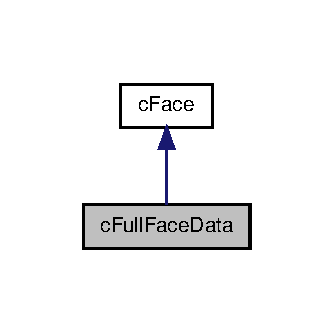
\includegraphics[width=160pt]{classc_full_face_data__inherit__graph}
\end{center}
\end{figure}


Collaboration diagram for cFullFaceData:
\nopagebreak
\begin{figure}[H]
\begin{center}
\leavevmode
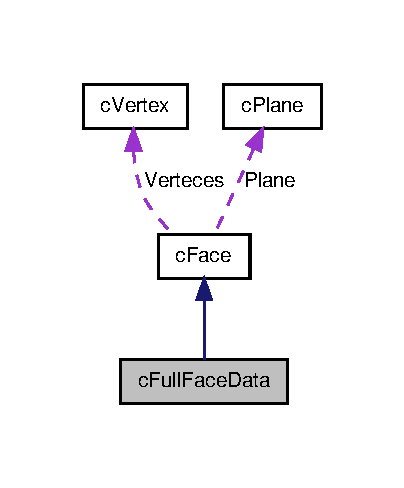
\includegraphics[width=194pt]{classc_full_face_data__coll__graph}
\end{center}
\end{figure}
\subsection*{Public Member Functions}
\begin{DoxyCompactItemize}
\item 
\hyperlink{classc_full_face_data_a63302db2911c4cace838a43347b79167}{cFullFaceData} ()
\item 
uint32 \hyperlink{classc_full_face_data_a53a99ced9de4ecdede38b2e8d63458e9}{FileSize} ()
\item 
void \hyperlink{classc_full_face_data_a8098f4af2f6d152bf27e4d8692421ce9}{Fill} (float $\ast$lpVertex, uint16 $\ast$mpFace)
\begin{DoxyCompactList}\small\item\em Will Fill the data for this Object from a array of floats representing vertex coordinates (3 floats to a vertex) and an array of 3 uint16s indicating which verteces to use. \item\end{DoxyCompactList}\item 
bool \hyperlink{classc_full_face_data_a9397eb74f9f3dd7fb82ec85c7cb291f5}{SamePlane} (\hyperlink{classc_plane}{cPlane} \&lpOther)
\begin{DoxyCompactList}\small\item\em Will return 1 if the \hyperlink{classc_plane}{cPlane} lpOther is in the same plane as this object. \item\end{DoxyCompactList}\item 
\hyperlink{classc_full_face_data}{cFullFaceData} \& \hyperlink{classc_full_face_data_a7a9bdcb3c4795ed42582aceb5624c04b}{operator=} (\hyperlink{classc_full_face_data}{cFullFaceData} \&lpOther)
\begin{DoxyCompactList}\small\item\em = operator \item\end{DoxyCompactList}\item 
bool \hyperlink{classc_full_face_data_adc17fbda36ec28287c88dccb893b23d5}{IsConcave} (\hyperlink{classc_full_face_list}{cFullFaceList} \&lpOther)
\begin{DoxyCompactList}\small\item\em Will return one if this Face is concave with the first connected cFullFace it is touching. \item\end{DoxyCompactList}\item 
bool \hyperlink{classc_full_face_data_ae05debbc355b5c55669e4f836780a7f8}{IsConcave} (\hyperlink{classc_face}{cFace} lpOther)
\begin{DoxyCompactList}\small\item\em Will return 1 if this Face is concave (and shares an edge) with the \hyperlink{classc_face}{cFace} lpOther. \item\end{DoxyCompactList}\item 
uint8 \hyperlink{classc_full_face_data_a625231204c052ebf231c2a1029776c90}{NotSharedVertex} (\hyperlink{classc_face}{cFace} \&lpOther)
\begin{DoxyCompactList}\small\item\em Will return the number of the Vertex owned by lpOther which is not shared by this face (0,1,2). If all faces are shared, will return 3. If no faces are shared will return 2. \item\end{DoxyCompactList}\item 
uint8 \hyperlink{classc_full_face_data_a836ca82086bc8b6301d7536d8aa51a45}{SharesVertex} (\hyperlink{classc_vertex}{cVertex} $\ast$lpOther)
\begin{DoxyCompactList}\small\item\em Will return the number of verteces that this object shares with the array of 3 \hyperlink{classc_vertex}{cVertex} object pointed to by lpOther (0,1,2,3). \item\end{DoxyCompactList}\item 
void \hyperlink{classc_full_face_data_a3792250bc347ccd2dc480bfc36550d3c}{OutputIMFFullFace} (ofstream \&FileStream)
\item 
void \hyperlink{classc_full_face_data_a0c4e4d07909a7896d21b69229cd10ac9}{LoadIMFFullFace} (ifstream \&FileStream)
\item 
void \hyperlink{classc_full_face_data_afc0dbbf171729f20ce08d9cea72f821c}{Display} ()
\begin{DoxyCompactList}\small\item\em Will output this object to the terminal. \item\end{DoxyCompactList}\end{DoxyCompactItemize}


\subsection{Detailed Description}
This class is a \hyperlink{classc_face}{cFace} with expanded Functionality. Allows the user to check information about the face. See list of functions for information. 

Definition at line 7 of file WTcFullFaceData.h.



\subsection{Constructor \& Destructor Documentation}
\hypertarget{classc_full_face_data_a63302db2911c4cace838a43347b79167}{
\index{cFullFaceData@{cFullFaceData}!cFullFaceData@{cFullFaceData}}
\index{cFullFaceData@{cFullFaceData}!cFullFaceData@{cFullFaceData}}
\subsubsection[{cFullFaceData}]{\setlength{\rightskip}{0pt plus 5cm}cFullFaceData::cFullFaceData (
\begin{DoxyParamCaption}
{}
\end{DoxyParamCaption}
)}}
\label{classc_full_face_data_a63302db2911c4cace838a43347b79167}


Definition at line 174 of file WTcFullFaceData.cpp.



\subsection{Member Function Documentation}
\hypertarget{classc_full_face_data_afc0dbbf171729f20ce08d9cea72f821c}{
\index{cFullFaceData@{cFullFaceData}!Display@{Display}}
\index{Display@{Display}!cFullFaceData@{cFullFaceData}}
\subsubsection[{Display}]{\setlength{\rightskip}{0pt plus 5cm}void cFullFaceData::Display (
\begin{DoxyParamCaption}
{}
\end{DoxyParamCaption}
)}}
\label{classc_full_face_data_afc0dbbf171729f20ce08d9cea72f821c}


Will output this object to the terminal. 



Definition at line 34 of file WTcFullFaceData.cpp.

\hypertarget{classc_full_face_data_a53a99ced9de4ecdede38b2e8d63458e9}{
\index{cFullFaceData@{cFullFaceData}!FileSize@{FileSize}}
\index{FileSize@{FileSize}!cFullFaceData@{cFullFaceData}}
\subsubsection[{FileSize}]{\setlength{\rightskip}{0pt plus 5cm}uint32 cFullFaceData::FileSize (
\begin{DoxyParamCaption}
{}
\end{DoxyParamCaption}
)}}
\label{classc_full_face_data_a53a99ced9de4ecdede38b2e8d63458e9}


Reimplemented from \hyperlink{classc_face_ac2da0ca5e4269e12016b74c6443cde32}{cFace}.



Definition at line 3 of file WTcFullFaceData.cpp.

\hypertarget{classc_full_face_data_a8098f4af2f6d152bf27e4d8692421ce9}{
\index{cFullFaceData@{cFullFaceData}!Fill@{Fill}}
\index{Fill@{Fill}!cFullFaceData@{cFullFaceData}}
\subsubsection[{Fill}]{\setlength{\rightskip}{0pt plus 5cm}void cFullFaceData::Fill (
\begin{DoxyParamCaption}
\item[{float $\ast$}]{lpVertex, }
\item[{uint16 $\ast$}]{mpFace}
\end{DoxyParamCaption}
)}}
\label{classc_full_face_data_a8098f4af2f6d152bf27e4d8692421ce9}


Will Fill the data for this Object from a array of floats representing vertex coordinates (3 floats to a vertex) and an array of 3 uint16s indicating which verteces to use. 



Definition at line 43 of file WTcFullFaceData.cpp.

\hypertarget{classc_full_face_data_adc17fbda36ec28287c88dccb893b23d5}{
\index{cFullFaceData@{cFullFaceData}!IsConcave@{IsConcave}}
\index{IsConcave@{IsConcave}!cFullFaceData@{cFullFaceData}}
\subsubsection[{IsConcave}]{\setlength{\rightskip}{0pt plus 5cm}bool cFullFaceData::IsConcave (
\begin{DoxyParamCaption}
\item[{{\bf cFullFaceList} \&}]{lpOther}
\end{DoxyParamCaption}
)}}
\label{classc_full_face_data_adc17fbda36ec28287c88dccb893b23d5}


Will return one if this Face is concave with the first connected cFullFace it is touching. 



Definition at line 77 of file WTcFullFaceData.cpp.

\hypertarget{classc_full_face_data_ae05debbc355b5c55669e4f836780a7f8}{
\index{cFullFaceData@{cFullFaceData}!IsConcave@{IsConcave}}
\index{IsConcave@{IsConcave}!cFullFaceData@{cFullFaceData}}
\subsubsection[{IsConcave}]{\setlength{\rightskip}{0pt plus 5cm}bool cFullFaceData::IsConcave (
\begin{DoxyParamCaption}
\item[{{\bf cFace}}]{lpOther}
\end{DoxyParamCaption}
)}}
\label{classc_full_face_data_ae05debbc355b5c55669e4f836780a7f8}


Will return 1 if this Face is concave (and shares an edge) with the \hyperlink{classc_face}{cFace} lpOther. 



Definition at line 109 of file WTcFullFaceData.cpp.

\hypertarget{classc_full_face_data_a0c4e4d07909a7896d21b69229cd10ac9}{
\index{cFullFaceData@{cFullFaceData}!LoadIMFFullFace@{LoadIMFFullFace}}
\index{LoadIMFFullFace@{LoadIMFFullFace}!cFullFaceData@{cFullFaceData}}
\subsubsection[{LoadIMFFullFace}]{\setlength{\rightskip}{0pt plus 5cm}void cFullFaceData::LoadIMFFullFace (
\begin{DoxyParamCaption}
\item[{ifstream \&}]{FileStream}
\end{DoxyParamCaption}
)}}
\label{classc_full_face_data_a0c4e4d07909a7896d21b69229cd10ac9}


Definition at line 25 of file WTcFullFaceData.cpp.

\hypertarget{classc_full_face_data_a625231204c052ebf231c2a1029776c90}{
\index{cFullFaceData@{cFullFaceData}!NotSharedVertex@{NotSharedVertex}}
\index{NotSharedVertex@{NotSharedVertex}!cFullFaceData@{cFullFaceData}}
\subsubsection[{NotSharedVertex}]{\setlength{\rightskip}{0pt plus 5cm}uint8 cFullFaceData::NotSharedVertex (
\begin{DoxyParamCaption}
\item[{{\bf cFace} \&}]{lpOther}
\end{DoxyParamCaption}
)}}
\label{classc_full_face_data_a625231204c052ebf231c2a1029776c90}


Will return the number of the Vertex owned by lpOther which is not shared by this face (0,1,2). If all faces are shared, will return 3. If no faces are shared will return 2. 



Definition at line 95 of file WTcFullFaceData.cpp.

\hypertarget{classc_full_face_data_a7a9bdcb3c4795ed42582aceb5624c04b}{
\index{cFullFaceData@{cFullFaceData}!operator=@{operator=}}
\index{operator=@{operator=}!cFullFaceData@{cFullFaceData}}
\subsubsection[{operator=}]{\setlength{\rightskip}{0pt plus 5cm}{\bf cFullFaceData} \& cFullFaceData::operator= (
\begin{DoxyParamCaption}
\item[{{\bf cFullFaceData} \&}]{lpOther}
\end{DoxyParamCaption}
)}}
\label{classc_full_face_data_a7a9bdcb3c4795ed42582aceb5624c04b}


= operator 



Definition at line 68 of file WTcFullFaceData.cpp.

\hypertarget{classc_full_face_data_a3792250bc347ccd2dc480bfc36550d3c}{
\index{cFullFaceData@{cFullFaceData}!OutputIMFFullFace@{OutputIMFFullFace}}
\index{OutputIMFFullFace@{OutputIMFFullFace}!cFullFaceData@{cFullFaceData}}
\subsubsection[{OutputIMFFullFace}]{\setlength{\rightskip}{0pt plus 5cm}void cFullFaceData::OutputIMFFullFace (
\begin{DoxyParamCaption}
\item[{ofstream \&}]{FileStream}
\end{DoxyParamCaption}
)}}
\label{classc_full_face_data_a3792250bc347ccd2dc480bfc36550d3c}


Definition at line 16 of file WTcFullFaceData.cpp.

\hypertarget{classc_full_face_data_a9397eb74f9f3dd7fb82ec85c7cb291f5}{
\index{cFullFaceData@{cFullFaceData}!SamePlane@{SamePlane}}
\index{SamePlane@{SamePlane}!cFullFaceData@{cFullFaceData}}
\subsubsection[{SamePlane}]{\setlength{\rightskip}{0pt plus 5cm}bool cFullFaceData::SamePlane (
\begin{DoxyParamCaption}
\item[{{\bf cPlane} \&}]{lpOther}
\end{DoxyParamCaption}
)}}
\label{classc_full_face_data_a9397eb74f9f3dd7fb82ec85c7cb291f5}


Will return 1 if the \hyperlink{classc_plane}{cPlane} lpOther is in the same plane as this object. 



Definition at line 63 of file WTcFullFaceData.cpp.

\hypertarget{classc_full_face_data_a836ca82086bc8b6301d7536d8aa51a45}{
\index{cFullFaceData@{cFullFaceData}!SharesVertex@{SharesVertex}}
\index{SharesVertex@{SharesVertex}!cFullFaceData@{cFullFaceData}}
\subsubsection[{SharesVertex}]{\setlength{\rightskip}{0pt plus 5cm}uint8 cFullFaceData::SharesVertex (
\begin{DoxyParamCaption}
\item[{{\bf cVertex} $\ast$}]{lpOther}
\end{DoxyParamCaption}
)}}
\label{classc_full_face_data_a836ca82086bc8b6301d7536d8aa51a45}


Will return the number of verteces that this object shares with the array of 3 \hyperlink{classc_vertex}{cVertex} object pointed to by lpOther (0,1,2,3). 



Definition at line 53 of file WTcFullFaceData.cpp.


\hypertarget{classc_full_face_list}{
\section{cFullFaceList Class Reference}
\label{classc_full_face_list}\index{cFullFaceList@{cFullFaceList}}
}


A dynamic linked list of \hyperlink{classc_full_face_data}{cFullFaceData}. As described. Can load object to and from IMFs.  




Inheritance diagram for cFullFaceList:
\nopagebreak
\begin{figure}[H]
\begin{center}
\leavevmode
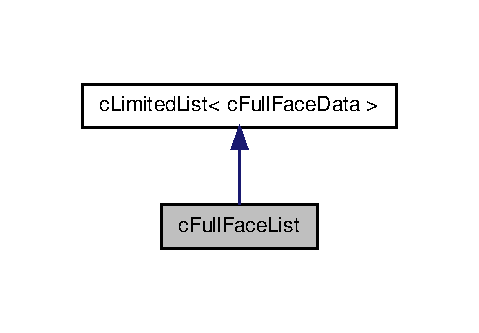
\includegraphics[width=230pt]{classc_full_face_list__inherit__graph}
\end{center}
\end{figure}


Collaboration diagram for cFullFaceList:
\nopagebreak
\begin{figure}[H]
\begin{center}
\leavevmode
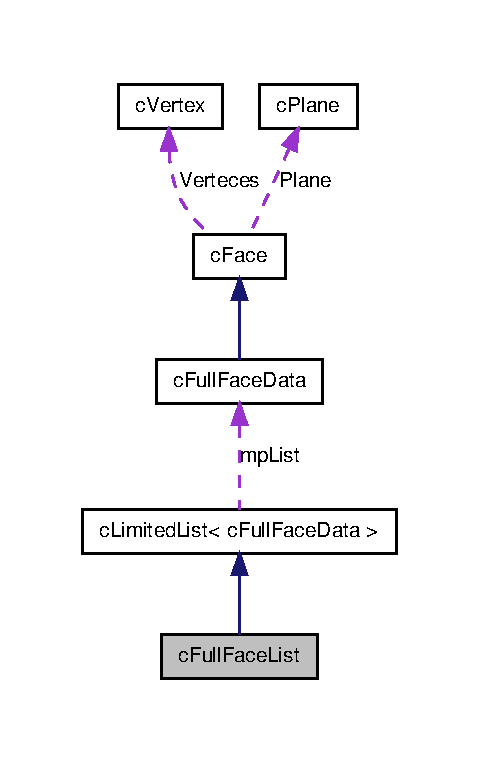
\includegraphics[width=230pt]{classc_full_face_list__coll__graph}
\end{center}
\end{figure}
\subsection*{Public Member Functions}
\begin{DoxyCompactItemize}
\item 
\hyperlink{classc_full_face_list_ad2b34976fbe03234f1cb5b7ec47d0a6a}{cFullFaceList} ()
\item 
\hyperlink{classc_full_face_list_ab911b30f55f2eb83f83cb1c6db71f177}{$\sim$cFullFaceList} ()
\item 
void \hyperlink{classc_full_face_list_ab8eeb41fd4ac55ad1e52bd9a243c079b}{OutputIMFFullFaces} (ofstream \&FileStream)
\item 
void \hyperlink{classc_full_face_list_a98005d8b47c59d90c0a8be70262fd037}{LoadIMFFullFaces} (ifstream \&FileStream)
\item 
uint32 \hyperlink{classc_full_face_list_a5eca55b7cdd11d560b2393a9dfae8269}{FileSize} ()
\item 
void \hyperlink{classc_full_face_list_a8ae1301cb5a95eb615499503041db454}{Display} ()
\item 
void \hyperlink{classc_full_face_list_a142e4c7546ea2d6872b2ddb3a31e8cc4}{Normalise} ()
\begin{DoxyCompactList}\small\item\em Will Normalise all Normals of the \hyperlink{classc_full_face_data}{cFullFaceData} objects in the list. \item\end{DoxyCompactList}\end{DoxyCompactItemize}


\subsection{Detailed Description}
A dynamic linked list of \hyperlink{classc_full_face_data}{cFullFaceData}. As described. Can load object to and from IMFs. 

Definition at line 46 of file WTcFullFaceData.h.



\subsection{Constructor \& Destructor Documentation}
\hypertarget{classc_full_face_list_ad2b34976fbe03234f1cb5b7ec47d0a6a}{
\index{cFullFaceList@{cFullFaceList}!cFullFaceList@{cFullFaceList}}
\index{cFullFaceList@{cFullFaceList}!cFullFaceList@{cFullFaceList}}
\subsubsection[{cFullFaceList}]{\setlength{\rightskip}{0pt plus 5cm}cFullFaceList::cFullFaceList (
\begin{DoxyParamCaption}
{}
\end{DoxyParamCaption}
)}}
\label{classc_full_face_list_ad2b34976fbe03234f1cb5b7ec47d0a6a}


Definition at line 171 of file WTcFullFaceData.cpp.

\hypertarget{classc_full_face_list_ab911b30f55f2eb83f83cb1c6db71f177}{
\index{cFullFaceList@{cFullFaceList}!$\sim$cFullFaceList@{$\sim$cFullFaceList}}
\index{$\sim$cFullFaceList@{$\sim$cFullFaceList}!cFullFaceList@{cFullFaceList}}
\subsubsection[{$\sim$cFullFaceList}]{\setlength{\rightskip}{0pt plus 5cm}cFullFaceList::$\sim$cFullFaceList (
\begin{DoxyParamCaption}
{}
\end{DoxyParamCaption}
)}}
\label{classc_full_face_list_ab911b30f55f2eb83f83cb1c6db71f177}


Definition at line 172 of file WTcFullFaceData.cpp.



\subsection{Member Function Documentation}
\hypertarget{classc_full_face_list_a8ae1301cb5a95eb615499503041db454}{
\index{cFullFaceList@{cFullFaceList}!Display@{Display}}
\index{Display@{Display}!cFullFaceList@{cFullFaceList}}
\subsubsection[{Display}]{\setlength{\rightskip}{0pt plus 5cm}void cFullFaceList::Display (
\begin{DoxyParamCaption}
{}
\end{DoxyParamCaption}
)}}
\label{classc_full_face_list_a8ae1301cb5a95eb615499503041db454}


Definition at line 152 of file WTcFullFaceData.cpp.

\hypertarget{classc_full_face_list_a5eca55b7cdd11d560b2393a9dfae8269}{
\index{cFullFaceList@{cFullFaceList}!FileSize@{FileSize}}
\index{FileSize@{FileSize}!cFullFaceList@{cFullFaceList}}
\subsubsection[{FileSize}]{\setlength{\rightskip}{0pt plus 5cm}uint32 cFullFaceList::FileSize (
\begin{DoxyParamCaption}
{}
\end{DoxyParamCaption}
)}}
\label{classc_full_face_list_a5eca55b7cdd11d560b2393a9dfae8269}


Definition at line 140 of file WTcFullFaceData.cpp.

\hypertarget{classc_full_face_list_a98005d8b47c59d90c0a8be70262fd037}{
\index{cFullFaceList@{cFullFaceList}!LoadIMFFullFaces@{LoadIMFFullFaces}}
\index{LoadIMFFullFaces@{LoadIMFFullFaces}!cFullFaceList@{cFullFaceList}}
\subsubsection[{LoadIMFFullFaces}]{\setlength{\rightskip}{0pt plus 5cm}void cFullFaceList::LoadIMFFullFaces (
\begin{DoxyParamCaption}
\item[{ifstream \&}]{FileStream}
\end{DoxyParamCaption}
)}}
\label{classc_full_face_list_a98005d8b47c59d90c0a8be70262fd037}


Definition at line 128 of file WTcFullFaceData.cpp.

\hypertarget{classc_full_face_list_a142e4c7546ea2d6872b2ddb3a31e8cc4}{
\index{cFullFaceList@{cFullFaceList}!Normalise@{Normalise}}
\index{Normalise@{Normalise}!cFullFaceList@{cFullFaceList}}
\subsubsection[{Normalise}]{\setlength{\rightskip}{0pt plus 5cm}void cFullFaceList::Normalise (
\begin{DoxyParamCaption}
{}
\end{DoxyParamCaption}
)}}
\label{classc_full_face_list_a142e4c7546ea2d6872b2ddb3a31e8cc4}


Will Normalise all Normals of the \hyperlink{classc_full_face_data}{cFullFaceData} objects in the list. 



Definition at line 162 of file WTcFullFaceData.cpp.

\hypertarget{classc_full_face_list_ab8eeb41fd4ac55ad1e52bd9a243c079b}{
\index{cFullFaceList@{cFullFaceList}!OutputIMFFullFaces@{OutputIMFFullFaces}}
\index{OutputIMFFullFaces@{OutputIMFFullFaces}!cFullFaceList@{cFullFaceList}}
\subsubsection[{OutputIMFFullFaces}]{\setlength{\rightskip}{0pt plus 5cm}void cFullFaceList::OutputIMFFullFaces (
\begin{DoxyParamCaption}
\item[{ofstream \&}]{FileStream}
\end{DoxyParamCaption}
)}}
\label{classc_full_face_list_ab8eeb41fd4ac55ad1e52bd9a243c079b}


Definition at line 118 of file WTcFullFaceData.cpp.


\hypertarget{classc_gravity_particle}{
\section{cGravityParticle Class Reference}
\label{classc_gravity_particle}\index{cGravityParticle@{cGravityParticle}}
}


cParticles which are affected by Gravity. These Particles have the code to be affected by the variables \_\-GRAVITY\_\-X,\_\-GRAVITY\_\-Y and \_\-GRAVITY\_\-Z. UpdatePos() will account use the current Gravity settings to calculate the speed and position.  


\subsection*{Friends}
\begin{DoxyCompactItemize}
\item 
\hypertarget{classc_gravity_particle_ad810bc5f0330a0154ffaabe8d256379c}{
class \hyperlink{classc_gravity_particle_ad810bc5f0330a0154ffaabe8d256379c}{cParticleHandler}}
\label{classc_gravity_particle_ad810bc5f0330a0154ffaabe8d256379c}

\end{DoxyCompactItemize}


\subsection{Detailed Description}
cParticles which are affected by Gravity. These Particles have the code to be affected by the variables \_\-GRAVITY\_\-X,\_\-GRAVITY\_\-Y and \_\-GRAVITY\_\-Z. UpdatePos() will account use the current Gravity settings to calculate the speed and position. 
\hypertarget{classc_image}{
\section{cImage Class Reference}
\label{classc_image}\index{cImage@{cImage}}
}


A 2D renderable object.  




Collaboration diagram for cImage:\nopagebreak
\begin{figure}[H]
\begin{center}
\leavevmode
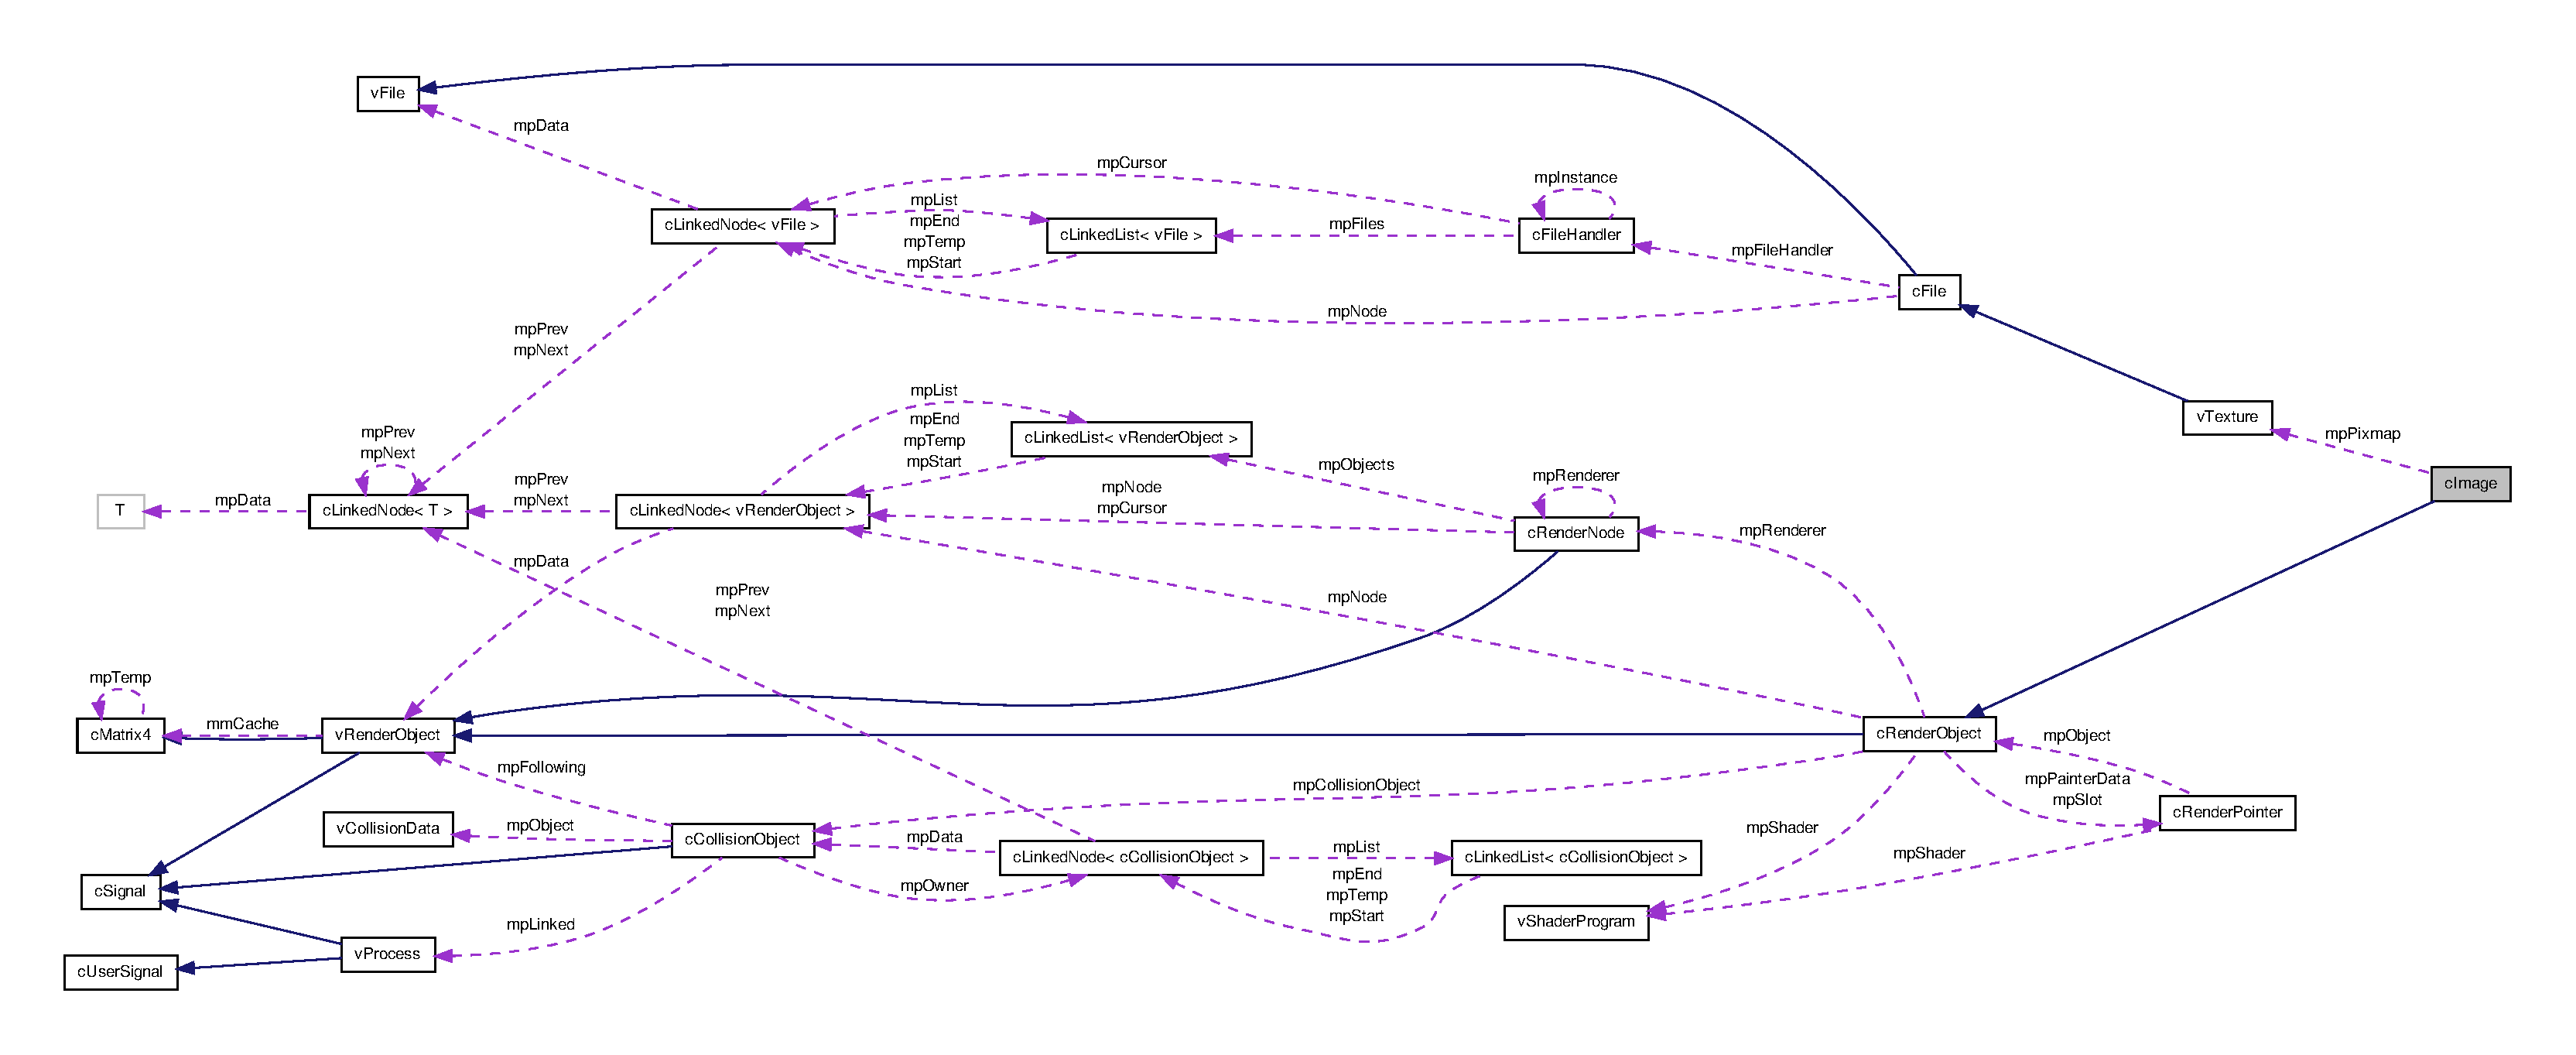
\includegraphics[width=400pt]{classc_image__coll__graph}
\end{center}
\end{figure}
\subsection*{Public Member Functions}
\begin{DoxyCompactItemize}
\item 
\hypertarget{classc_image_a7acf286a86645d8acb39a7b02b06ac0a}{
\hyperlink{classc_image_a7acf286a86645d8acb39a7b02b06ac0a}{cImage} ()}
\label{classc_image_a7acf286a86645d8acb39a7b02b06ac0a}

\begin{DoxyCompactList}\small\item\em Constructor for \hyperlink{classc_image}{cImage}. Will Create an Empty \hyperlink{classc_image}{cImage} Object. \end{DoxyCompactList}\item 
\hypertarget{classc_image_a39864db63ddc349351463e511b7ab433}{
virtual void \hyperlink{classc_image_a39864db63ddc349351463e511b7ab433}{Size} (float lfSize)}
\label{classc_image_a39864db63ddc349351463e511b7ab433}

\begin{DoxyCompactList}\small\item\em Sets the size of the image on screen. Makes the width be lfSize pixels and makes the height to make it appear square. \end{DoxyCompactList}\item 
\hypertarget{classc_image_a3abd5e2a010875c08e08add7e224008e}{
virtual void \hyperlink{classc_image_a3abd5e2a010875c08e08add7e224008e}{Width} (float lfWidth)}
\label{classc_image_a3abd5e2a010875c08e08add7e224008e}

\begin{DoxyCompactList}\small\item\em Sets the size of the image on screen. Makes the width be lfSize pixels and makes the height to make it appear square. \end{DoxyCompactList}\item 
\hypertarget{classc_image_a165ba2ed14e5bf1913357f34ca3a9403}{
virtual void \hyperlink{classc_image_a165ba2ed14e5bf1913357f34ca3a9403}{Height} (float lfHeight)}
\label{classc_image_a165ba2ed14e5bf1913357f34ca3a9403}

\begin{DoxyCompactList}\small\item\em Sets the size of the image on screen. Makes the width be lfSize pixels and makes the height to make it appear square. \end{DoxyCompactList}\item 
\hypertarget{classc_image_aacc1a4884b4fc04b936a1695a393d26a}{
float \hyperlink{classc_image_aacc1a4884b4fc04b936a1695a393d26a}{Width} ()}
\label{classc_image_aacc1a4884b4fc04b936a1695a393d26a}

\begin{DoxyCompactList}\small\item\em Will return the Width of this image in pixels. \end{DoxyCompactList}\item 
\hypertarget{classc_image_adfccfa4a2893b805bf231d5039c27f05}{
float \hyperlink{classc_image_adfccfa4a2893b805bf231d5039c27f05}{Height} ()}
\label{classc_image_adfccfa4a2893b805bf231d5039c27f05}

\begin{DoxyCompactList}\small\item\em Will return the Height of this image in pixels. \end{DoxyCompactList}\end{DoxyCompactItemize}
\subsection*{Friends}
\begin{DoxyCompactItemize}
\item 
\hypertarget{classc_image_ac3e18951e9137b17e506e36253a11cb7}{
class \hyperlink{classc_image_ac3e18951e9137b17e506e36253a11cb7}{cImage3D}}
\label{classc_image_ac3e18951e9137b17e506e36253a11cb7}

\end{DoxyCompactItemize}


\subsection{Detailed Description}
A 2D renderable object. 


\begin{DoxyParams}{Parameters}
{\em lpTexture} & pointer to the texture to bind to this 2D object This is actually a 3D polygon, which has a texture bound to it. it can be used as an OpenGL accelerated sprite. \\
\hline
\end{DoxyParams}

\hypertarget{classc_i_m_f_loader}{
\section{cIMFLoader Class Reference}
\label{classc_i_m_f_loader}\index{cIMFLoader@{cIMFLoader}}
}


Inheritance diagram for cIMFLoader:
\nopagebreak
\begin{figure}[H]
\begin{center}
\leavevmode
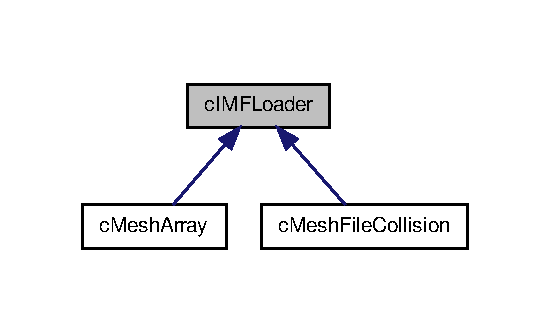
\includegraphics[width=264pt]{classc_i_m_f_loader__inherit__graph}
\end{center}
\end{figure}
\subsection*{Public Member Functions}
\begin{DoxyCompactItemize}
\item 
void \hyperlink{classc_i_m_f_loader_a219c95a2cfbb5f477b10d9158f77470c}{LoadIMF} (ifstream \&FileStream)
\end{DoxyCompactItemize}


\subsection{Detailed Description}


Definition at line 4 of file WTcIMFLoader.h.



\subsection{Member Function Documentation}
\hypertarget{classc_i_m_f_loader_a219c95a2cfbb5f477b10d9158f77470c}{
\index{cIMFLoader@{cIMFLoader}!LoadIMF@{LoadIMF}}
\index{LoadIMF@{LoadIMF}!cIMFLoader@{cIMFLoader}}
\subsubsection[{LoadIMF}]{\setlength{\rightskip}{0pt plus 5cm}void cIMFLoader::LoadIMF (
\begin{DoxyParamCaption}
\item[{ifstream \&}]{FileStream}
\end{DoxyParamCaption}
)}}
\label{classc_i_m_f_loader_a219c95a2cfbb5f477b10d9158f77470c}


Reimplemented in \hyperlink{classc_mesh_file_collision_ac40c927ae3dfecfb2c9a0e40fbcd31b3}{cMeshFileCollision}, and \hyperlink{classc_mesh_array_adce4a1c4b77569227f23d1e4cc46b4bb}{cMeshArray}.


\hypertarget{classc_kernel}{
\section{cKernel Class Reference}
\label{classc_kernel}\index{cKernel@{cKernel}}
}


Kernel Object. Handles Processes. Tracks, runs and deletes current processes. Has complete control over every \hyperlink{classc_process}{cProcess} object. Will run all awake alive processes every process cycle, will delete dead processes. Also controls the activation of rendering frames and handling interactions with the operating system.  




Collaboration diagram for cKernel:
\nopagebreak
\begin{figure}[H]
\begin{center}
\leavevmode
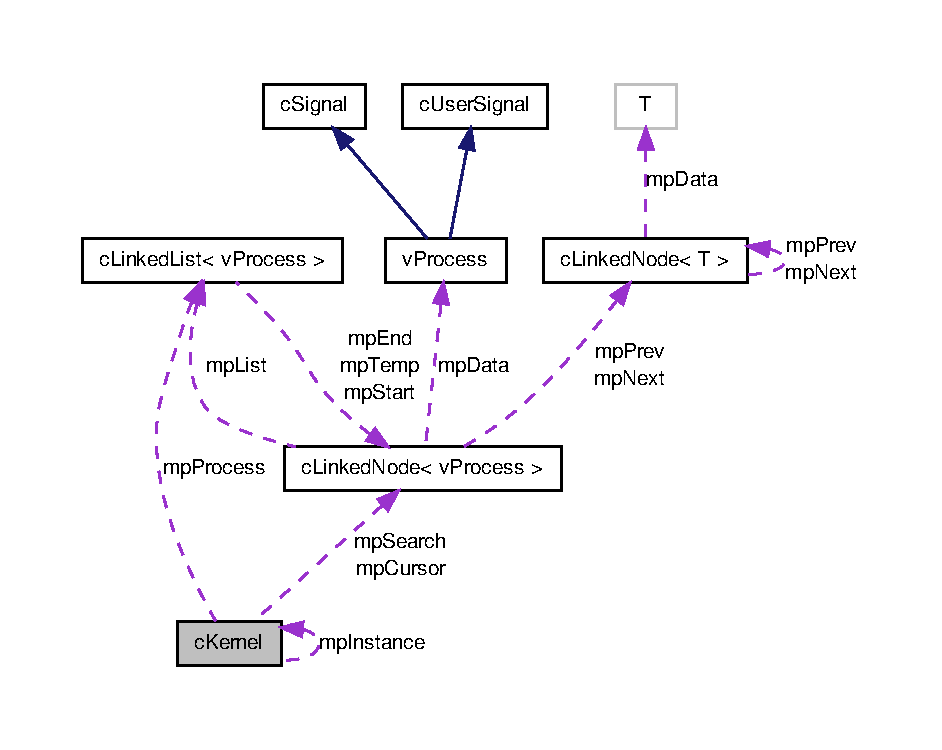
\includegraphics[width=400pt]{classc_kernel__coll__graph}
\end{center}
\end{figure}
\subsection*{Public Member Functions}
\begin{DoxyCompactItemize}
\item 
void \hyperlink{classc_kernel_a721f5ad665c512b511ff8d344010385e}{KillProgram} ()
\begin{DoxyCompactList}\small\item\em Will kill the entire program. Will delete every process and then exit. \item\end{DoxyCompactList}\item 
\hyperlink{classc_kernel_aa17d85bb9118c9de59fe0c6301301a39}{$\sim$cKernel} ()
\item 
void \hyperlink{classc_kernel_afbbf3ca5d7f5db9c91f1c279c0109b2f}{Update} ()
\item 
\hyperlink{classc_linked_node}{cLinkedNode}$<$ \hyperlink{classv_process}{vProcess} $>$ $\ast$ \hyperlink{classc_kernel_a4ec4faedede9de3cae4fc5fbc4469a1b}{Add} (\hyperlink{classv_process}{vProcess} $\ast$lpNew)
\item 
void \hyperlink{classc_kernel_a59c9a956e6a6666a57c2d85e463381d8}{Remove} (\hyperlink{classc_linked_node}{cLinkedNode}$<$ \hyperlink{classv_process}{vProcess} $>$ $\ast$lpOld)
\item 
void \hyperlink{classc_kernel_af4c3e32a55fdef58236378eed46afdfe}{DeleteAll} ()
\begin{DoxyCompactList}\small\item\em Will Delete all the processes in the current process list. This will effectively end the program. \item\end{DoxyCompactList}\item 
{\footnotesize template$<$class tType $>$ }\\tType $\ast$ \hyperlink{classc_kernel_a56083c090177a8a2a9bb50ad58e712c3}{FindProcess} ()
\begin{DoxyCompactList}\small\item\em This Function will search for a process of either tType OR a type which has uses the type tType as a base type. \item\end{DoxyCompactList}\item 
void \hyperlink{classc_kernel_a42d5d224af7acfe4aee27b7cee2b0a02}{ResetFindProcess} ()
\begin{DoxyCompactList}\small\item\em This Function will reset \hyperlink{classc_kernel_a56083c090177a8a2a9bb50ad58e712c3}{FindProcess()} to search from the start of the process List. \item\end{DoxyCompactList}\end{DoxyCompactItemize}
\subsection*{Static Public Member Functions}
\begin{DoxyCompactItemize}
\item 
static \hyperlink{classc_kernel}{cKernel} $\ast$ \hyperlink{classc_kernel_a5bd65ef494632b9fd585a6f6cae375e7}{Instance} ()
\begin{DoxyCompactList}\small\item\em Function which returns current Kernel Instance. Will Create a new instance if one does not already exist. \item\end{DoxyCompactList}\end{DoxyCompactItemize}


\subsection{Detailed Description}
Kernel Object. Handles Processes. Tracks, runs and deletes current processes. Has complete control over every \hyperlink{classc_process}{cProcess} object. Will run all awake alive processes every process cycle, will delete dead processes. Also controls the activation of rendering frames and handling interactions with the operating system. 

Definition at line 15 of file WTKernel.h.



\subsection{Constructor \& Destructor Documentation}
\hypertarget{classc_kernel_aa17d85bb9118c9de59fe0c6301301a39}{
\index{cKernel@{cKernel}!$\sim$cKernel@{$\sim$cKernel}}
\index{$\sim$cKernel@{$\sim$cKernel}!cKernel@{cKernel}}
\subsubsection[{$\sim$cKernel}]{\setlength{\rightskip}{0pt plus 5cm}cKernel::$\sim$cKernel (
\begin{DoxyParamCaption}
{}
\end{DoxyParamCaption}
)}}
\label{classc_kernel_aa17d85bb9118c9de59fe0c6301301a39}


Definition at line 94 of file WTKernel.cpp.



\subsection{Member Function Documentation}
\hypertarget{classc_kernel_a4ec4faedede9de3cae4fc5fbc4469a1b}{
\index{cKernel@{cKernel}!Add@{Add}}
\index{Add@{Add}!cKernel@{cKernel}}
\subsubsection[{Add}]{\setlength{\rightskip}{0pt plus 5cm}{\bf cLinkedNode}$<$ {\bf vProcess} $>$ $\ast$ cKernel::Add (
\begin{DoxyParamCaption}
\item[{{\bf vProcess} $\ast$}]{lpNew}
\end{DoxyParamCaption}
)}}
\label{classc_kernel_a4ec4faedede9de3cae4fc5fbc4469a1b}


Definition at line 123 of file WTKernel.cpp.

\hypertarget{classc_kernel_af4c3e32a55fdef58236378eed46afdfe}{
\index{cKernel@{cKernel}!DeleteAll@{DeleteAll}}
\index{DeleteAll@{DeleteAll}!cKernel@{cKernel}}
\subsubsection[{DeleteAll}]{\setlength{\rightskip}{0pt plus 5cm}void cKernel::DeleteAll (
\begin{DoxyParamCaption}
{}
\end{DoxyParamCaption}
)}}
\label{classc_kernel_af4c3e32a55fdef58236378eed46afdfe}


Will Delete all the processes in the current process list. This will effectively end the program. 



Definition at line 12 of file WTKernel.cpp.

\hypertarget{classc_kernel_a56083c090177a8a2a9bb50ad58e712c3}{
\index{cKernel@{cKernel}!FindProcess@{FindProcess}}
\index{FindProcess@{FindProcess}!cKernel@{cKernel}}
\subsubsection[{FindProcess}]{\setlength{\rightskip}{0pt plus 5cm}template$<$class tType $>$ tType $\ast$ cKernel::FindProcess (
\begin{DoxyParamCaption}
{}
\end{DoxyParamCaption}
)}}
\label{classc_kernel_a56083c090177a8a2a9bb50ad58e712c3}


This Function will search for a process of either tType OR a type which has uses the type tType as a base type. 


\begin{DoxyParams}{Parameters}
{\em mpType} & is a pointer of the type (or base type) of the desired process. \\
\hline
\end{DoxyParams}
\begin{DoxyReturn}{Returns}
Will return a pointer to a process currently in the process list of the correct type.
\end{DoxyReturn}
This Function takes the type of the pointer handed to the function and will search for a process which is of type tType or inherits tType. Can be used to find processes of a certain type or genus. Each call of this function will continue searching from the position stored in mpSearch. Between searches for processes of different types use the function \hyperlink{classc_kernel_a42d5d224af7acfe4aee27b7cee2b0a02}{ResetFindProcess()}. 
\begin{DoxyCode}
        cGunShip *mpGunShip;
        cBattleShip *mpBattleShip;

        mpGunShip = FindProcess(mpGunShip);
        ResetFindProcess();
        mpBattleShip = FindProcess(mpBattleShip);
\end{DoxyCode}
 

Definition at line 92 of file WTKernel.h.

\hypertarget{classc_kernel_a5bd65ef494632b9fd585a6f6cae375e7}{
\index{cKernel@{cKernel}!Instance@{Instance}}
\index{Instance@{Instance}!cKernel@{cKernel}}
\subsubsection[{Instance}]{\setlength{\rightskip}{0pt plus 5cm}{\bf cKernel} $\ast$ cKernel::Instance (
\begin{DoxyParamCaption}
{}
\end{DoxyParamCaption}
)\hspace{0.3cm}{\ttfamily  \mbox{[}static\mbox{]}}}}
\label{classc_kernel_a5bd65ef494632b9fd585a6f6cae375e7}


Function which returns current Kernel Instance. Will Create a new instance if one does not already exist. 



Definition at line 139 of file WTKernel.cpp.

\hypertarget{classc_kernel_a721f5ad665c512b511ff8d344010385e}{
\index{cKernel@{cKernel}!KillProgram@{KillProgram}}
\index{KillProgram@{KillProgram}!cKernel@{cKernel}}
\subsubsection[{KillProgram}]{\setlength{\rightskip}{0pt plus 5cm}void cKernel::KillProgram (
\begin{DoxyParamCaption}
{}
\end{DoxyParamCaption}
)}}
\label{classc_kernel_a721f5ad665c512b511ff8d344010385e}


Will kill the entire program. Will delete every process and then exit. 



Definition at line 162 of file WTKernel.cpp.

\hypertarget{classc_kernel_a59c9a956e6a6666a57c2d85e463381d8}{
\index{cKernel@{cKernel}!Remove@{Remove}}
\index{Remove@{Remove}!cKernel@{cKernel}}
\subsubsection[{Remove}]{\setlength{\rightskip}{0pt plus 5cm}void cKernel::Remove (
\begin{DoxyParamCaption}
\item[{{\bf cLinkedNode}$<$ {\bf vProcess} $>$ $\ast$}]{lpOld}
\end{DoxyParamCaption}
)}}
\label{classc_kernel_a59c9a956e6a6666a57c2d85e463381d8}


Definition at line 134 of file WTKernel.cpp.

\hypertarget{classc_kernel_a42d5d224af7acfe4aee27b7cee2b0a02}{
\index{cKernel@{cKernel}!ResetFindProcess@{ResetFindProcess}}
\index{ResetFindProcess@{ResetFindProcess}!cKernel@{cKernel}}
\subsubsection[{ResetFindProcess}]{\setlength{\rightskip}{0pt plus 5cm}void cKernel::ResetFindProcess (
\begin{DoxyParamCaption}
{}
\end{DoxyParamCaption}
)}}
\label{classc_kernel_a42d5d224af7acfe4aee27b7cee2b0a02}


This Function will reset \hyperlink{classc_kernel_a56083c090177a8a2a9bb50ad58e712c3}{FindProcess()} to search from the start of the process List. 



Definition at line 160 of file WTKernel.cpp.

\hypertarget{classc_kernel_afbbf3ca5d7f5db9c91f1c279c0109b2f}{
\index{cKernel@{cKernel}!Update@{Update}}
\index{Update@{Update}!cKernel@{cKernel}}
\subsubsection[{Update}]{\setlength{\rightskip}{0pt plus 5cm}void cKernel::Update (
\begin{DoxyParamCaption}
{}
\end{DoxyParamCaption}
)}}
\label{classc_kernel_afbbf3ca5d7f5db9c91f1c279c0109b2f}


Definition at line 18 of file WTKernel.cpp.


\hypertarget{classc_key_store}{
\section{cKeyStore Class Reference}
\label{classc_key_store}\index{cKeyStore@{cKeyStore}}
}


This class stores all the input data for a single keyboard.  


\subsection*{Public Member Functions}
\begin{DoxyCompactItemize}
\item 
\hypertarget{classc_key_store_a338766086dd09a48b8cefd33fb35bc7a}{
\hyperlink{classc_key_store_a338766086dd09a48b8cefd33fb35bc7a}{cKeyStore} ()}
\label{classc_key_store_a338766086dd09a48b8cefd33fb35bc7a}

\begin{DoxyCompactList}\small\item\em This will return a specific key state, using the relevant key code. \end{DoxyCompactList}\end{DoxyCompactItemize}
\subsection*{Public Attributes}
\begin{DoxyCompactItemize}
\item 
\hypertarget{classc_key_store_a1b0760ec36eafb3c3ef74b21e60e4009}{
bool \hyperlink{classc_key_store_a1b0760ec36eafb3c3ef74b21e60e4009}{key} \mbox{[}2\mbox{]}\mbox{[}256\mbox{]}}
\label{classc_key_store_a1b0760ec36eafb3c3ef74b21e60e4009}

\begin{DoxyCompactList}\small\item\em This is the array of keystates. \end{DoxyCompactList}\end{DoxyCompactItemize}


\subsection{Detailed Description}
This class stores all the input data for a single keyboard. 
\hypertarget{classc_landscape}{
\section{cLandscape Class Reference}
\label{classc_landscape}\index{cLandscape@{cLandscape}}
}


A height map based, matrix structured Landscape. Landscape is composed of a matrix of square polygons. The heights of each vertex is produced using the packaging software, and is generated from a bitmap.  




Collaboration diagram for cLandscape:\nopagebreak
\begin{figure}[H]
\begin{center}
\leavevmode
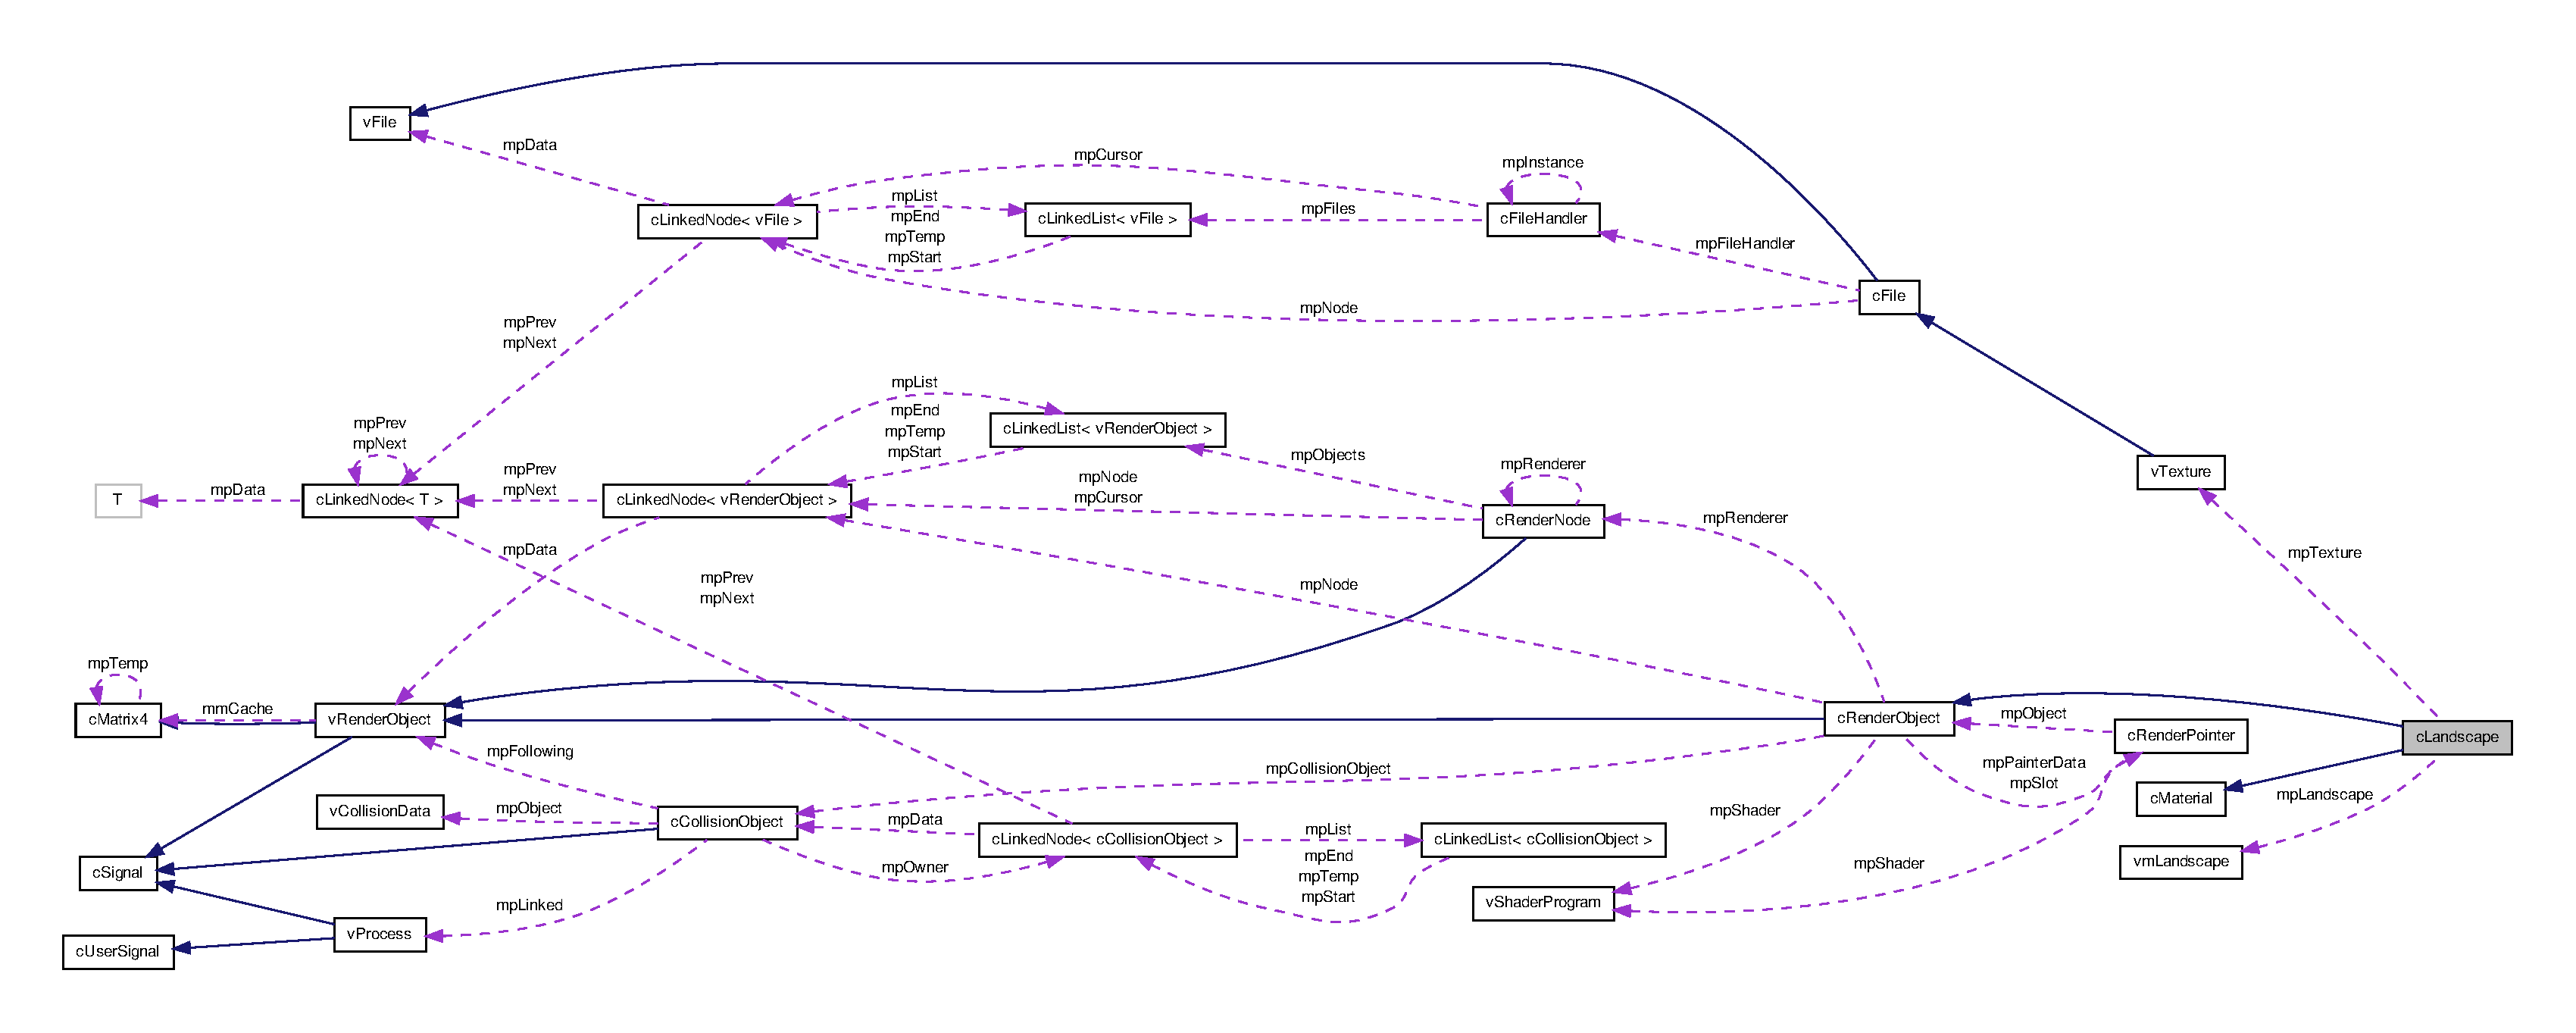
\includegraphics[width=400pt]{classc_landscape__coll__graph}
\end{center}
\end{figure}
\subsection*{Public Member Functions}
\begin{DoxyCompactItemize}
\item 
\hypertarget{classc_landscape_afc86bc9f2d3ce929abc8ef5e6dcd1248}{
\hyperlink{classc_landscape_afc86bc9f2d3ce929abc8ef5e6dcd1248}{cLandscape} (\hyperlink{classcm_landscape}{cmLandscape} $\ast$lpModel, \hyperlink{classc_camera}{cCamera} $\ast$lpCamera)}
\label{classc_landscape_afc86bc9f2d3ce929abc8ef5e6dcd1248}

\begin{DoxyCompactList}\small\item\em Create a landscape object and set its height map and texture. Can also assign the Landscape to a Camera. \end{DoxyCompactList}\item 
\hypertarget{classc_landscape_a1fa3ad374cf96116beb5791cc9aa713e}{
\hyperlink{classc_landscape_a1fa3ad374cf96116beb5791cc9aa713e}{cLandscape} (\hyperlink{classcm_landscape}{cmLandscape} $\ast$lpModel=0)}
\label{classc_landscape_a1fa3ad374cf96116beb5791cc9aa713e}

\begin{DoxyCompactList}\small\item\em Create a landscape object and set its height map and texture. \end{DoxyCompactList}\item 
\hypertarget{classc_landscape_ac945c88a536fee7dd2f499e199225939}{
void \hyperlink{classc_landscape_ac945c88a536fee7dd2f499e199225939}{Landscape} (\hyperlink{classcm_landscape}{cmLandscape} $\ast$lpLandscape)}
\label{classc_landscape_ac945c88a536fee7dd2f499e199225939}

\begin{DoxyCompactList}\small\item\em Set the current height map for this landscape object. \end{DoxyCompactList}\item 
\hypertarget{classc_landscape_ae30d44a1e780ef4f120c4aa4dc460c06}{
void \hyperlink{classc_landscape_ae30d44a1e780ef4f120c4aa4dc460c06}{Landscape} (string lsLandscape)}
\label{classc_landscape_ae30d44a1e780ef4f120c4aa4dc460c06}

\begin{DoxyCompactList}\small\item\em Set the current height map for this landscape object to use. \end{DoxyCompactList}\item 
\hypertarget{classc_landscape_a36f6a35064d14d460f99464181c5c830}{
float \hyperlink{classc_landscape_a36f6a35064d14d460f99464181c5c830}{GetHeight} (float lfX, float lfZ)}
\label{classc_landscape_a36f6a35064d14d460f99464181c5c830}

\begin{DoxyCompactList}\small\item\em Will return the height at Global co-\/ordinates lfX,lfZ. \end{DoxyCompactList}\item 
\hypertarget{classc_landscape_acdb3f590236a85b1423acc47f064e9b7}{
float \hyperlink{classc_landscape_acdb3f590236a85b1423acc47f064e9b7}{GetHeightLocal} (float lfX, float lfZ)}
\label{classc_landscape_acdb3f590236a85b1423acc47f064e9b7}

\begin{DoxyCompactList}\small\item\em Will return the height at the Local position lfX,lfZ (relative to landscapes corner) \end{DoxyCompactList}\item 
\hypertarget{classc_landscape_a7642e8b5062010778a1ad8913077a661}{
float \hyperlink{classc_landscape_a7642e8b5062010778a1ad8913077a661}{GetVertexHeight} (int liX, int liZ)}
\label{classc_landscape_a7642e8b5062010778a1ad8913077a661}

\begin{DoxyCompactList}\small\item\em Will return the height of the vertex at liX,liZ. (position is based on number of segments NOT distance) \end{DoxyCompactList}\end{DoxyCompactItemize}


\subsection{Detailed Description}
A height map based, matrix structured Landscape. Landscape is composed of a matrix of square polygons. The heights of each vertex is produced using the packaging software, and is generated from a bitmap. 
\hypertarget{classc_landscape_mesh_file}{
\section{cLandscapeMeshFile Class Reference}
\label{classc_landscape_mesh_file}\index{cLandscapeMeshFile@{cLandscapeMeshFile}}
}


This is the class which the Landscape File is stored in. This can be passed to any of \hyperlink{classcm_landscape}{cmLandscape}, cLandscapeMeshIndividual or cLandscapeMeshRandom.  




Collaboration diagram for cLandscapeMeshFile:\nopagebreak
\begin{figure}[H]
\begin{center}
\leavevmode
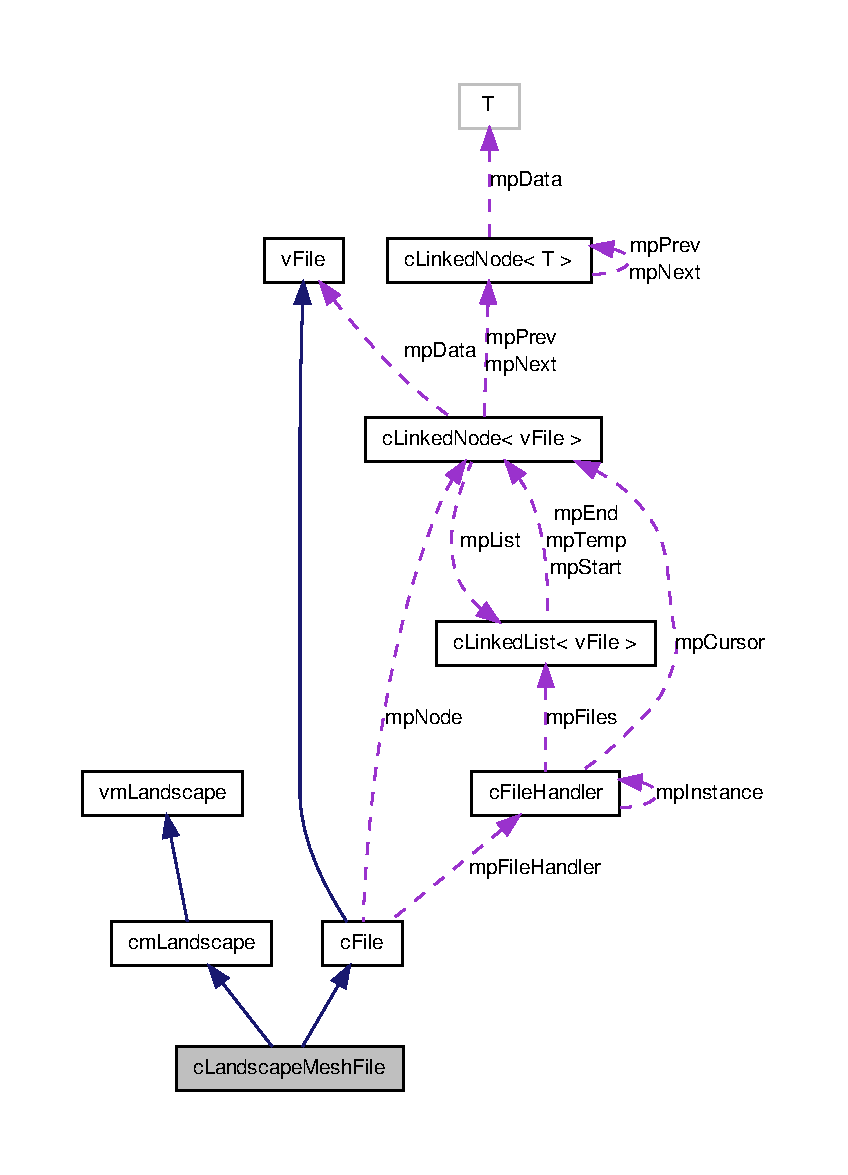
\includegraphics[width=378pt]{classc_landscape_mesh_file__coll__graph}
\end{center}
\end{figure}
\subsection*{Friends}
\begin{DoxyCompactItemize}
\item 
\hypertarget{classc_landscape_mesh_file_a642b5e78056302f99f656983a53beb6d}{
class \hyperlink{classc_landscape_mesh_file_a642b5e78056302f99f656983a53beb6d}{cmLandscape}}
\label{classc_landscape_mesh_file_a642b5e78056302f99f656983a53beb6d}

\end{DoxyCompactItemize}


\subsection{Detailed Description}
This is the class which the Landscape File is stored in. This can be passed to any of \hyperlink{classcm_landscape}{cmLandscape}, cLandscapeMeshIndividual or cLandscapeMeshRandom. 
\hypertarget{classc_light}{
\section{cLight Class Reference}
\label{classc_light}\index{cLight@{cLight}}
}


Creates an OpenGL light effect.  




Inheritance diagram for cLight:
\nopagebreak
\begin{figure}[H]
\begin{center}
\leavevmode
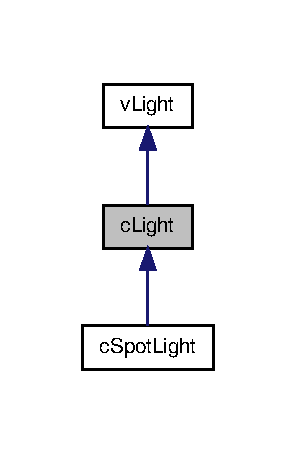
\includegraphics[width=142pt]{classc_light__inherit__graph}
\end{center}
\end{figure}


Collaboration diagram for cLight:
\nopagebreak
\begin{figure}[H]
\begin{center}
\leavevmode
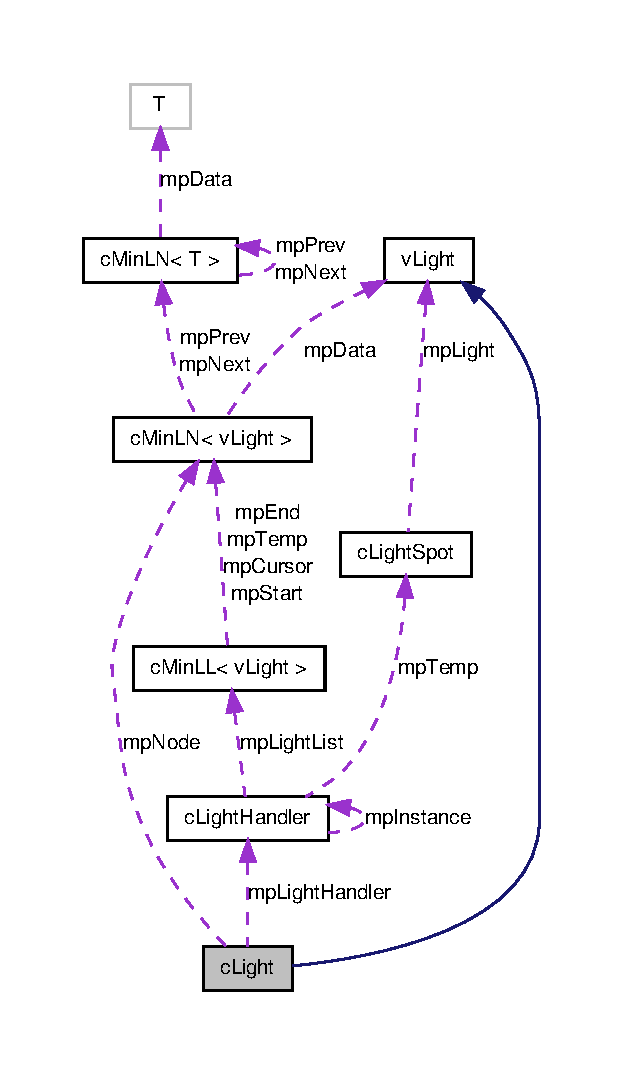
\includegraphics[width=299pt]{classc_light__coll__graph}
\end{center}
\end{figure}
\subsection*{Public Member Functions}
\begin{DoxyCompactItemize}
\item 
\hyperlink{classc_light_a695d9165a904e1b6ffedbef6fa8cc955}{cLight} ()
\begin{DoxyCompactList}\small\item\em Constructor, will create a new light source. \item\end{DoxyCompactList}\item 
\hyperlink{classc_light_a3354570a7b1a8b5a484b84d3b231a87e}{$\sim$cLight} ()
\item 
void \hyperlink{classc_light_a71f44adf2794e62eba33c58db557d057}{Position} (float lfX, float lfY, float lfZ)
\begin{DoxyCompactList}\small\item\em Will Move the light to Global position lfX,lfY,lfZ. \item\end{DoxyCompactList}\item 
float $\ast$ \hyperlink{classc_light_adee1be4882423cd78568a0ab3ec01e5b}{Position} ()
\begin{DoxyCompactList}\small\item\em Will Return the Current position of the light. \item\end{DoxyCompactList}\item 
void \hyperlink{classc_light_af8ece4e5cf59812835eeb6ca80c485c2}{Ambient} (float lfR, float lfG, float lfB, float lfA)
\begin{DoxyCompactList}\small\item\em Will set the Ambient light color for the light source (RGBA). \item\end{DoxyCompactList}\item 
void \hyperlink{classc_light_a74ae85e3b13ddc3b31a01257f9810e66}{Diffuse} (float lfR, float lfG, float lfB, float lfA)
\begin{DoxyCompactList}\small\item\em Will set the Diffuse light color for the light source (RGBA). \item\end{DoxyCompactList}\item 
void \hyperlink{classc_light_a0c9fac24be43f1b053e3ff8ecc89cd28}{Specular} (float lfR, float lfG, float lfB, float lfA)
\begin{DoxyCompactList}\small\item\em Will set the Specular light color for the light source (RGBA). \item\end{DoxyCompactList}\item 
virtual void \hyperlink{classc_light_a2dccfde2dd2dab941d58762f8c56b1a9}{PrepareLight} ()
\begin{DoxyCompactList}\small\item\em Will bind this light source for use in OpenGL. Once all the Lights Variables are set, call this to preapre the light. \item\end{DoxyCompactList}\item 
virtual void \hyperlink{classc_light_a9a67a4ca727ffe13ff04a87385a14e0e}{PrepareLight} (uint32 liLight)
\item 
void \hyperlink{classc_light_a9f4ef9ebd121db8ce0f23a113d48f218}{Attenuation} (float liAttenuation)
\begin{DoxyCompactList}\small\item\em Will Set the value for the attenuation factor. \item\end{DoxyCompactList}\item 
void \hyperlink{classc_light_a8394ef099b87c18df58759c8431ab084}{AttenuationType} (uint8 liOrder)
\begin{DoxyCompactList}\small\item\em Will Set the order of the attenuation (0=constant, 1=linear or 2=Quadratic). \item\end{DoxyCompactList}\item 
void \hyperlink{classc_light_a9f6bd610b772e5185fa948dfec91d865}{SetID} (uint8 liLightID)
\begin{DoxyCompactList}\small\item\em Will Set the Lights ID (The OpenGL light number this light will render to by default). \item\end{DoxyCompactList}\end{DoxyCompactItemize}
\subsection*{Protected Attributes}
\begin{DoxyCompactItemize}
\item 
uint8 \hyperlink{classc_light_a0a636a1b5d3068e44d71ed4f5e58c86c}{miLightID}
\item 
float \hyperlink{classc_light_a5f4f6e1a73a23d7c7d7402316cf91459}{mpPosition} \mbox{[}4\mbox{]}
\item 
float \hyperlink{classc_light_a69a6e96ee70410b23201aa0eacb50326}{mpAmbient} \mbox{[}4\mbox{]}
\item 
float \hyperlink{classc_light_aa9c9538d45ce0ba6bb0c36b257c609e9}{mpDiffuse} \mbox{[}4\mbox{]}
\item 
float \hyperlink{classc_light_aceff329257be92835c2962e77ad2d3dc}{mpSpecular} \mbox{[}4\mbox{]}
\item 
float \hyperlink{classc_light_a1c5452dfe39ff550f30be8727d2862fc}{miAttenuation}
\item 
uint32 \hyperlink{classc_light_af266e29e6bbfee100a480a911c6bbee4}{miAttenuationType}
\item 
\hyperlink{classc_min_l_n}{cMinLN}$<$ \hyperlink{classv_light}{vLight} $>$ $\ast$ \hyperlink{classc_light_a6e718feeaad0a71e8654f85142bae362}{mpNode}
\end{DoxyCompactItemize}
\subsection*{Static Protected Attributes}
\begin{DoxyCompactItemize}
\item 
static \hyperlink{classc_light_handler}{cLightHandler} $\ast$ \hyperlink{classc_light_adb4d7d2b2d8d5e832bee031e70a87fd6}{mpLightHandler} = 0
\end{DoxyCompactItemize}


\subsection{Detailed Description}
Creates an OpenGL light effect. 

Definition at line 4 of file WTcLight.h.



\subsection{Constructor \& Destructor Documentation}
\hypertarget{classc_light_a695d9165a904e1b6ffedbef6fa8cc955}{
\index{cLight@{cLight}!cLight@{cLight}}
\index{cLight@{cLight}!cLight@{cLight}}
\subsubsection[{cLight}]{\setlength{\rightskip}{0pt plus 5cm}cLight::cLight (
\begin{DoxyParamCaption}
{}
\end{DoxyParamCaption}
)}}
\label{classc_light_a695d9165a904e1b6ffedbef6fa8cc955}


Constructor, will create a new light source. 



Definition at line 15 of file WTcLight.cpp.

\hypertarget{classc_light_a3354570a7b1a8b5a484b84d3b231a87e}{
\index{cLight@{cLight}!$\sim$cLight@{$\sim$cLight}}
\index{$\sim$cLight@{$\sim$cLight}!cLight@{cLight}}
\subsubsection[{$\sim$cLight}]{\setlength{\rightskip}{0pt plus 5cm}cLight::$\sim$cLight (
\begin{DoxyParamCaption}
{}
\end{DoxyParamCaption}
)}}
\label{classc_light_a3354570a7b1a8b5a484b84d3b231a87e}


Definition at line 3 of file WTcLight.cpp.



\subsection{Member Function Documentation}
\hypertarget{classc_light_af8ece4e5cf59812835eeb6ca80c485c2}{
\index{cLight@{cLight}!Ambient@{Ambient}}
\index{Ambient@{Ambient}!cLight@{cLight}}
\subsubsection[{Ambient}]{\setlength{\rightskip}{0pt plus 5cm}void cLight::Ambient (
\begin{DoxyParamCaption}
\item[{float}]{lfR, }
\item[{float}]{lfG, }
\item[{float}]{lfB, }
\item[{float}]{lfA}
\end{DoxyParamCaption}
)}}
\label{classc_light_af8ece4e5cf59812835eeb6ca80c485c2}


Will set the Ambient light color for the light source (RGBA). 



Definition at line 38 of file WTcLight.cpp.

\hypertarget{classc_light_a9f4ef9ebd121db8ce0f23a113d48f218}{
\index{cLight@{cLight}!Attenuation@{Attenuation}}
\index{Attenuation@{Attenuation}!cLight@{cLight}}
\subsubsection[{Attenuation}]{\setlength{\rightskip}{0pt plus 5cm}void cLight::Attenuation (
\begin{DoxyParamCaption}
\item[{float}]{liAttenuation}
\end{DoxyParamCaption}
)}}
\label{classc_light_a9f4ef9ebd121db8ce0f23a113d48f218}


Will Set the value for the attenuation factor. 



Definition at line 87 of file WTcLight.cpp.

\hypertarget{classc_light_a8394ef099b87c18df58759c8431ab084}{
\index{cLight@{cLight}!AttenuationType@{AttenuationType}}
\index{AttenuationType@{AttenuationType}!cLight@{cLight}}
\subsubsection[{AttenuationType}]{\setlength{\rightskip}{0pt plus 5cm}void cLight::AttenuationType (
\begin{DoxyParamCaption}
\item[{uint8}]{liOrder}
\end{DoxyParamCaption}
)}}
\label{classc_light_a8394ef099b87c18df58759c8431ab084}


Will Set the order of the attenuation (0=constant, 1=linear or 2=Quadratic). 



Definition at line 82 of file WTcLight.cpp.

\hypertarget{classc_light_a74ae85e3b13ddc3b31a01257f9810e66}{
\index{cLight@{cLight}!Diffuse@{Diffuse}}
\index{Diffuse@{Diffuse}!cLight@{cLight}}
\subsubsection[{Diffuse}]{\setlength{\rightskip}{0pt plus 5cm}void cLight::Diffuse (
\begin{DoxyParamCaption}
\item[{float}]{lfR, }
\item[{float}]{lfG, }
\item[{float}]{lfB, }
\item[{float}]{lfA}
\end{DoxyParamCaption}
)}}
\label{classc_light_a74ae85e3b13ddc3b31a01257f9810e66}


Will set the Diffuse light color for the light source (RGBA). 



Definition at line 46 of file WTcLight.cpp.

\hypertarget{classc_light_adee1be4882423cd78568a0ab3ec01e5b}{
\index{cLight@{cLight}!Position@{Position}}
\index{Position@{Position}!cLight@{cLight}}
\subsubsection[{Position}]{\setlength{\rightskip}{0pt plus 5cm}float$\ast$ cLight::Position (
\begin{DoxyParamCaption}
{}
\end{DoxyParamCaption}
)\hspace{0.3cm}{\ttfamily  \mbox{[}inline, virtual\mbox{]}}}}
\label{classc_light_adee1be4882423cd78568a0ab3ec01e5b}


Will Return the Current position of the light. 



Implements \hyperlink{classv_light_a8b01a4aabfe76a8c0c2806fa5084a12b}{vLight}.



Definition at line 37 of file WTcLight.h.

\hypertarget{classc_light_a71f44adf2794e62eba33c58db557d057}{
\index{cLight@{cLight}!Position@{Position}}
\index{Position@{Position}!cLight@{cLight}}
\subsubsection[{Position}]{\setlength{\rightskip}{0pt plus 5cm}void cLight::Position (
\begin{DoxyParamCaption}
\item[{float}]{lfX, }
\item[{float}]{lfY, }
\item[{float}]{lfZ}
\end{DoxyParamCaption}
)}}
\label{classc_light_a71f44adf2794e62eba33c58db557d057}


Will Move the light to Global position lfX,lfY,lfZ. 



Definition at line 29 of file WTcLight.cpp.

\hypertarget{classc_light_a9a67a4ca727ffe13ff04a87385a14e0e}{
\index{cLight@{cLight}!PrepareLight@{PrepareLight}}
\index{PrepareLight@{PrepareLight}!cLight@{cLight}}
\subsubsection[{PrepareLight}]{\setlength{\rightskip}{0pt plus 5cm}void cLight::PrepareLight (
\begin{DoxyParamCaption}
\item[{uint32}]{liLight}
\end{DoxyParamCaption}
)\hspace{0.3cm}{\ttfamily  \mbox{[}virtual\mbox{]}}}}
\label{classc_light_a9a67a4ca727ffe13ff04a87385a14e0e}


Implements \hyperlink{classv_light_aa71893aa279fc3742a516b289ab52848}{vLight}.



Reimplemented in \hyperlink{classc_spot_light_a576a95e7cb6c79007e23b4423198c751}{cSpotLight}.



Definition at line 72 of file WTcLight.cpp.

\hypertarget{classc_light_a2dccfde2dd2dab941d58762f8c56b1a9}{
\index{cLight@{cLight}!PrepareLight@{PrepareLight}}
\index{PrepareLight@{PrepareLight}!cLight@{cLight}}
\subsubsection[{PrepareLight}]{\setlength{\rightskip}{0pt plus 5cm}void cLight::PrepareLight (
\begin{DoxyParamCaption}
{}
\end{DoxyParamCaption}
)\hspace{0.3cm}{\ttfamily  \mbox{[}virtual\mbox{]}}}}
\label{classc_light_a2dccfde2dd2dab941d58762f8c56b1a9}


Will bind this light source for use in OpenGL. Once all the Lights Variables are set, call this to preapre the light. 



Implements \hyperlink{classv_light_a71d2a53a5ceaf14ee6bfa91ad5132177}{vLight}.



Reimplemented in \hyperlink{classc_spot_light_a364884b72b528981594b1440f6cbabcc}{cSpotLight}.



Definition at line 63 of file WTcLight.cpp.

\hypertarget{classc_light_a9f6bd610b772e5185fa948dfec91d865}{
\index{cLight@{cLight}!SetID@{SetID}}
\index{SetID@{SetID}!cLight@{cLight}}
\subsubsection[{SetID}]{\setlength{\rightskip}{0pt plus 5cm}void cLight::SetID (
\begin{DoxyParamCaption}
\item[{uint8}]{liLightID}
\end{DoxyParamCaption}
)\hspace{0.3cm}{\ttfamily  \mbox{[}virtual\mbox{]}}}}
\label{classc_light_a9f6bd610b772e5185fa948dfec91d865}


Will Set the Lights ID (The OpenGL light number this light will render to by default). 



Implements \hyperlink{classv_light_a4de112698fd63d5fc101366f43f540ca}{vLight}.



Definition at line 10 of file WTcLight.cpp.

\hypertarget{classc_light_a0c9fac24be43f1b053e3ff8ecc89cd28}{
\index{cLight@{cLight}!Specular@{Specular}}
\index{Specular@{Specular}!cLight@{cLight}}
\subsubsection[{Specular}]{\setlength{\rightskip}{0pt plus 5cm}void cLight::Specular (
\begin{DoxyParamCaption}
\item[{float}]{lfR, }
\item[{float}]{lfG, }
\item[{float}]{lfB, }
\item[{float}]{lfA}
\end{DoxyParamCaption}
)}}
\label{classc_light_a0c9fac24be43f1b053e3ff8ecc89cd28}


Will set the Specular light color for the light source (RGBA). 



Definition at line 54 of file WTcLight.cpp.



\subsection{Member Data Documentation}
\hypertarget{classc_light_a1c5452dfe39ff550f30be8727d2862fc}{
\index{cLight@{cLight}!miAttenuation@{miAttenuation}}
\index{miAttenuation@{miAttenuation}!cLight@{cLight}}
\subsubsection[{miAttenuation}]{\setlength{\rightskip}{0pt plus 5cm}float {\bf cLight::miAttenuation}\hspace{0.3cm}{\ttfamily  \mbox{[}protected\mbox{]}}}}
\label{classc_light_a1c5452dfe39ff550f30be8727d2862fc}


Definition at line 20 of file WTcLight.h.

\hypertarget{classc_light_af266e29e6bbfee100a480a911c6bbee4}{
\index{cLight@{cLight}!miAttenuationType@{miAttenuationType}}
\index{miAttenuationType@{miAttenuationType}!cLight@{cLight}}
\subsubsection[{miAttenuationType}]{\setlength{\rightskip}{0pt plus 5cm}uint32 {\bf cLight::miAttenuationType}\hspace{0.3cm}{\ttfamily  \mbox{[}protected\mbox{]}}}}
\label{classc_light_af266e29e6bbfee100a480a911c6bbee4}


Definition at line 22 of file WTcLight.h.

\hypertarget{classc_light_a0a636a1b5d3068e44d71ed4f5e58c86c}{
\index{cLight@{cLight}!miLightID@{miLightID}}
\index{miLightID@{miLightID}!cLight@{cLight}}
\subsubsection[{miLightID}]{\setlength{\rightskip}{0pt plus 5cm}uint8 {\bf cLight::miLightID}\hspace{0.3cm}{\ttfamily  \mbox{[}protected\mbox{]}}}}
\label{classc_light_a0a636a1b5d3068e44d71ed4f5e58c86c}


Definition at line 8 of file WTcLight.h.

\hypertarget{classc_light_a69a6e96ee70410b23201aa0eacb50326}{
\index{cLight@{cLight}!mpAmbient@{mpAmbient}}
\index{mpAmbient@{mpAmbient}!cLight@{cLight}}
\subsubsection[{mpAmbient}]{\setlength{\rightskip}{0pt plus 5cm}float {\bf cLight::mpAmbient}\mbox{[}4\mbox{]}\hspace{0.3cm}{\ttfamily  \mbox{[}protected\mbox{]}}}}
\label{classc_light_a69a6e96ee70410b23201aa0eacb50326}


Definition at line 13 of file WTcLight.h.

\hypertarget{classc_light_aa9c9538d45ce0ba6bb0c36b257c609e9}{
\index{cLight@{cLight}!mpDiffuse@{mpDiffuse}}
\index{mpDiffuse@{mpDiffuse}!cLight@{cLight}}
\subsubsection[{mpDiffuse}]{\setlength{\rightskip}{0pt plus 5cm}float {\bf cLight::mpDiffuse}\mbox{[}4\mbox{]}\hspace{0.3cm}{\ttfamily  \mbox{[}protected\mbox{]}}}}
\label{classc_light_aa9c9538d45ce0ba6bb0c36b257c609e9}


Definition at line 15 of file WTcLight.h.

\hypertarget{classc_light_adb4d7d2b2d8d5e832bee031e70a87fd6}{
\index{cLight@{cLight}!mpLightHandler@{mpLightHandler}}
\index{mpLightHandler@{mpLightHandler}!cLight@{cLight}}
\subsubsection[{mpLightHandler}]{\setlength{\rightskip}{0pt plus 5cm}{\bf cLightHandler} $\ast$ {\bf cLight::mpLightHandler} = 0\hspace{0.3cm}{\ttfamily  \mbox{[}static, protected\mbox{]}}}}
\label{classc_light_adb4d7d2b2d8d5e832bee031e70a87fd6}


Definition at line 24 of file WTcLight.h.

\hypertarget{classc_light_a6e718feeaad0a71e8654f85142bae362}{
\index{cLight@{cLight}!mpNode@{mpNode}}
\index{mpNode@{mpNode}!cLight@{cLight}}
\subsubsection[{mpNode}]{\setlength{\rightskip}{0pt plus 5cm}{\bf cMinLN}$<${\bf vLight}$>$$\ast$ {\bf cLight::mpNode}\hspace{0.3cm}{\ttfamily  \mbox{[}protected\mbox{]}}}}
\label{classc_light_a6e718feeaad0a71e8654f85142bae362}


Definition at line 25 of file WTcLight.h.

\hypertarget{classc_light_a5f4f6e1a73a23d7c7d7402316cf91459}{
\index{cLight@{cLight}!mpPosition@{mpPosition}}
\index{mpPosition@{mpPosition}!cLight@{cLight}}
\subsubsection[{mpPosition}]{\setlength{\rightskip}{0pt plus 5cm}float {\bf cLight::mpPosition}\mbox{[}4\mbox{]}\hspace{0.3cm}{\ttfamily  \mbox{[}protected\mbox{]}}}}
\label{classc_light_a5f4f6e1a73a23d7c7d7402316cf91459}


Definition at line 11 of file WTcLight.h.

\hypertarget{classc_light_aceff329257be92835c2962e77ad2d3dc}{
\index{cLight@{cLight}!mpSpecular@{mpSpecular}}
\index{mpSpecular@{mpSpecular}!cLight@{cLight}}
\subsubsection[{mpSpecular}]{\setlength{\rightskip}{0pt plus 5cm}float {\bf cLight::mpSpecular}\mbox{[}4\mbox{]}\hspace{0.3cm}{\ttfamily  \mbox{[}protected\mbox{]}}}}
\label{classc_light_aceff329257be92835c2962e77ad2d3dc}


Definition at line 17 of file WTcLight.h.


\hypertarget{classc_light_handler}{
\section{cLightHandler Class Reference}
\label{classc_light_handler}\index{cLightHandler@{cLightHandler}}
}


\hyperlink{classc_light_handler}{cLightHandler} will control the OpenGL Lights. It will turn off lights not required or possible for different renderings to increase speed and circumvent the OpenGL limit of active lights. OpenGL has a limited number of lights that can be used at any one time. This handler identifies the lights which will have the greatest effect on the current object and prepares the optimal selection of lights for rendering the scene.  




Collaboration diagram for cLightHandler:
\nopagebreak
\begin{figure}[H]
\begin{center}
\leavevmode
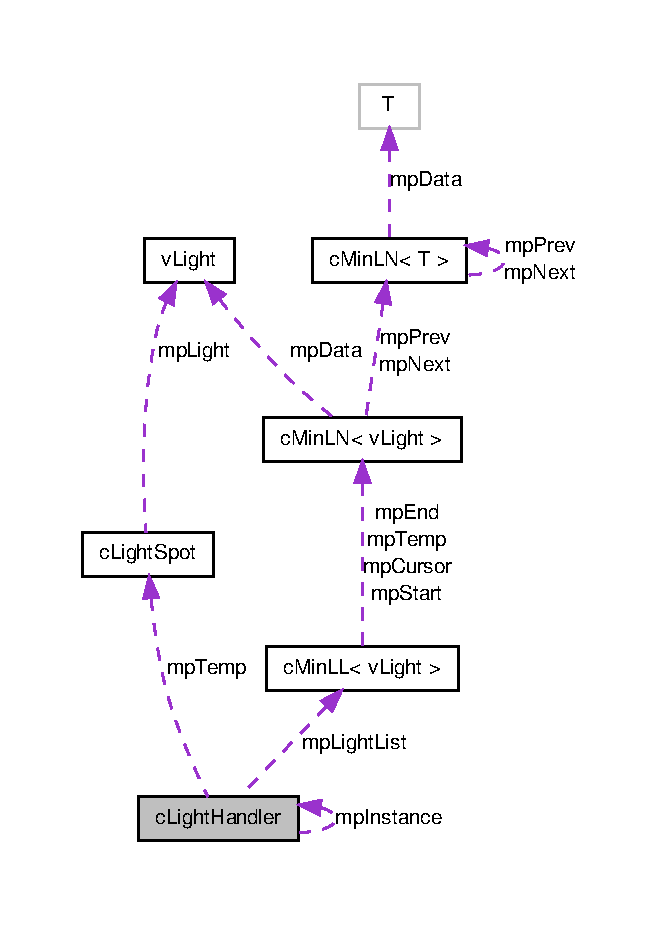
\includegraphics[width=317pt]{classc_light_handler__coll__graph}
\end{center}
\end{figure}
\subsection*{Public Member Functions}
\begin{DoxyCompactItemize}
\item 
\hyperlink{classc_light_handler_a17ed4af735943e71d486ebbe15b70eb8}{$\sim$cLightHandler} ()
\item 
\hyperlink{classc_min_l_n}{cMinLN}$<$ \hyperlink{classv_light}{vLight} $>$ $\ast$ \hyperlink{classc_light_handler_ad11b0b020fe2dbe57e0cdff69e4ccdbe}{Add} (\hyperlink{classv_light}{vLight} $\ast$lpNew)
\item 
void \hyperlink{classc_light_handler_a6961b97a431244a4494e36fe468b67fb}{PrepareLight} ()
\begin{DoxyCompactList}\small\item\em Will Prepare all the Lights for Rendering generally. \item\end{DoxyCompactList}\item 
void \hyperlink{classc_light_handler_af496ab1e05b26dcc1ae5da53a84da271}{PrepareLight} (\hyperlink{classc_matrix4}{cMatrix4} $\ast$mpObj)
\begin{DoxyCompactList}\small\item\em Will Prepare the Lights for Rendering a specific Object. \item\end{DoxyCompactList}\item 
void \hyperlink{classc_light_handler_a8c89de26ed57dca05e0daa5dbf089f8f}{Remove} (\hyperlink{classc_min_l_n}{cMinLN}$<$ \hyperlink{classv_light}{vLight} $>$ $\ast$lpOld)
\item 
void \hyperlink{classc_light_handler_aa3fa6f26deaa89361a703e94224bf641}{DeleteAll} ()
\begin{DoxyCompactList}\small\item\em Will Delete all the processes in the current Light list. \item\end{DoxyCompactList}\end{DoxyCompactItemize}
\subsection*{Static Public Member Functions}
\begin{DoxyCompactItemize}
\item 
static void \hyperlink{classc_light_handler_ac1357d0e2b0a15413a5a6b16e1b3abab}{SetupLights} ()
\item 
static \hyperlink{classc_light_handler}{cLightHandler} $\ast$ \hyperlink{classc_light_handler_ac0473959c255734fa3937f3d09e718a0}{Instance} ()
\begin{DoxyCompactList}\small\item\em This function will return a pointer to the current \hyperlink{classc_light_handler}{cLightHandler} Object. \item\end{DoxyCompactList}\end{DoxyCompactItemize}


\subsection{Detailed Description}
\hyperlink{classc_light_handler}{cLightHandler} will control the OpenGL Lights. It will turn off lights not required or possible for different renderings to increase speed and circumvent the OpenGL limit of active lights. OpenGL has a limited number of lights that can be used at any one time. This handler identifies the lights which will have the greatest effect on the current object and prepares the optimal selection of lights for rendering the scene. 

Definition at line 15 of file WTcLightHandler.h.



\subsection{Constructor \& Destructor Documentation}
\hypertarget{classc_light_handler_a17ed4af735943e71d486ebbe15b70eb8}{
\index{cLightHandler@{cLightHandler}!$\sim$cLightHandler@{$\sim$cLightHandler}}
\index{$\sim$cLightHandler@{$\sim$cLightHandler}!cLightHandler@{cLightHandler}}
\subsubsection[{$\sim$cLightHandler}]{\setlength{\rightskip}{0pt plus 5cm}cLightHandler::$\sim$cLightHandler (
\begin{DoxyParamCaption}
{}
\end{DoxyParamCaption}
)}}
\label{classc_light_handler_a17ed4af735943e71d486ebbe15b70eb8}


Definition at line 9 of file WTcLightHandler.cpp.



\subsection{Member Function Documentation}
\hypertarget{classc_light_handler_ad11b0b020fe2dbe57e0cdff69e4ccdbe}{
\index{cLightHandler@{cLightHandler}!Add@{Add}}
\index{Add@{Add}!cLightHandler@{cLightHandler}}
\subsubsection[{Add}]{\setlength{\rightskip}{0pt plus 5cm}{\bf cMinLN}$<$ {\bf vLight} $>$ $\ast$ cLightHandler::Add (
\begin{DoxyParamCaption}
\item[{{\bf vLight} $\ast$}]{lpNew}
\end{DoxyParamCaption}
)}}
\label{classc_light_handler_ad11b0b020fe2dbe57e0cdff69e4ccdbe}


Definition at line 36 of file WTcLightHandler.cpp.

\hypertarget{classc_light_handler_aa3fa6f26deaa89361a703e94224bf641}{
\index{cLightHandler@{cLightHandler}!DeleteAll@{DeleteAll}}
\index{DeleteAll@{DeleteAll}!cLightHandler@{cLightHandler}}
\subsubsection[{DeleteAll}]{\setlength{\rightskip}{0pt plus 5cm}void cLightHandler::DeleteAll (
\begin{DoxyParamCaption}
{}
\end{DoxyParamCaption}
)}}
\label{classc_light_handler_aa3fa6f26deaa89361a703e94224bf641}


Will Delete all the processes in the current Light list. 



Definition at line 50 of file WTcLightHandler.cpp.

\hypertarget{classc_light_handler_ac0473959c255734fa3937f3d09e718a0}{
\index{cLightHandler@{cLightHandler}!Instance@{Instance}}
\index{Instance@{Instance}!cLightHandler@{cLightHandler}}
\subsubsection[{Instance}]{\setlength{\rightskip}{0pt plus 5cm}{\bf cLightHandler} $\ast$ cLightHandler::Instance (
\begin{DoxyParamCaption}
{}
\end{DoxyParamCaption}
)\hspace{0.3cm}{\ttfamily  \mbox{[}static\mbox{]}}}}
\label{classc_light_handler_ac0473959c255734fa3937f3d09e718a0}


This function will return a pointer to the current \hyperlink{classc_light_handler}{cLightHandler} Object. 



Definition at line 18 of file WTcLightHandler.cpp.

\hypertarget{classc_light_handler_af496ab1e05b26dcc1ae5da53a84da271}{
\index{cLightHandler@{cLightHandler}!PrepareLight@{PrepareLight}}
\index{PrepareLight@{PrepareLight}!cLightHandler@{cLightHandler}}
\subsubsection[{PrepareLight}]{\setlength{\rightskip}{0pt plus 5cm}void cLightHandler::PrepareLight (
\begin{DoxyParamCaption}
\item[{{\bf cMatrix4} $\ast$}]{mpObj}
\end{DoxyParamCaption}
)}}
\label{classc_light_handler_af496ab1e05b26dcc1ae5da53a84da271}


Will Prepare the Lights for Rendering a specific Object. 



Definition at line 72 of file WTcLightHandler.cpp.

\hypertarget{classc_light_handler_a6961b97a431244a4494e36fe468b67fb}{
\index{cLightHandler@{cLightHandler}!PrepareLight@{PrepareLight}}
\index{PrepareLight@{PrepareLight}!cLightHandler@{cLightHandler}}
\subsubsection[{PrepareLight}]{\setlength{\rightskip}{0pt plus 5cm}void cLightHandler::PrepareLight (
\begin{DoxyParamCaption}
{}
\end{DoxyParamCaption}
)}}
\label{classc_light_handler_a6961b97a431244a4494e36fe468b67fb}


Will Prepare all the Lights for Rendering generally. 



Definition at line 61 of file WTcLightHandler.cpp.

\hypertarget{classc_light_handler_a8c89de26ed57dca05e0daa5dbf089f8f}{
\index{cLightHandler@{cLightHandler}!Remove@{Remove}}
\index{Remove@{Remove}!cLightHandler@{cLightHandler}}
\subsubsection[{Remove}]{\setlength{\rightskip}{0pt plus 5cm}void cLightHandler::Remove (
\begin{DoxyParamCaption}
\item[{{\bf cMinLN}$<$ {\bf vLight} $>$ $\ast$}]{lpOld}
\end{DoxyParamCaption}
)}}
\label{classc_light_handler_a8c89de26ed57dca05e0daa5dbf089f8f}


Definition at line 56 of file WTcLightHandler.cpp.

\hypertarget{classc_light_handler_ac1357d0e2b0a15413a5a6b16e1b3abab}{
\index{cLightHandler@{cLightHandler}!SetupLights@{SetupLights}}
\index{SetupLights@{SetupLights}!cLightHandler@{cLightHandler}}
\subsubsection[{SetupLights}]{\setlength{\rightskip}{0pt plus 5cm}void cLightHandler::SetupLights (
\begin{DoxyParamCaption}
{}
\end{DoxyParamCaption}
)\hspace{0.3cm}{\ttfamily  \mbox{[}static\mbox{]}}}}
\label{classc_light_handler_ac1357d0e2b0a15413a5a6b16e1b3abab}


Definition at line 24 of file WTcLightHandler.cpp.


\hypertarget{classc_light_spot}{
\section{cLightSpot Class Reference}
\label{classc_light_spot}\index{cLightSpot@{cLightSpot}}
}


Collaboration diagram for cLightSpot:
\nopagebreak
\begin{figure}[H]
\begin{center}
\leavevmode
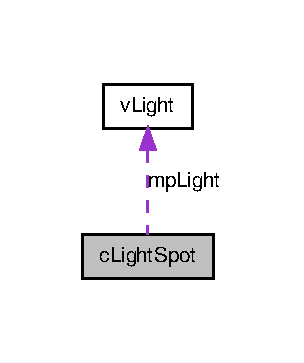
\includegraphics[width=146pt]{classc_light_spot__coll__graph}
\end{center}
\end{figure}
\subsection*{Public Attributes}
\begin{DoxyCompactItemize}
\item 
\hyperlink{classv_light}{vLight} $\ast$ \hyperlink{classc_light_spot_ab46df08134a9fdcd89db80b9f023cf52}{mpLight}
\item 
double \hyperlink{classc_light_spot_a1eeeb5aa72c52ae4ce85ab7ca83f6100}{mfDist}
\end{DoxyCompactItemize}


\subsection{Detailed Description}


Definition at line 4 of file WTcLightHandler.h.



\subsection{Member Data Documentation}
\hypertarget{classc_light_spot_a1eeeb5aa72c52ae4ce85ab7ca83f6100}{
\index{cLightSpot@{cLightSpot}!mfDist@{mfDist}}
\index{mfDist@{mfDist}!cLightSpot@{cLightSpot}}
\subsubsection[{mfDist}]{\setlength{\rightskip}{0pt plus 5cm}double {\bf cLightSpot::mfDist}}}
\label{classc_light_spot_a1eeeb5aa72c52ae4ce85ab7ca83f6100}


Definition at line 8 of file WTcLightHandler.h.

\hypertarget{classc_light_spot_ab46df08134a9fdcd89db80b9f023cf52}{
\index{cLightSpot@{cLightSpot}!mpLight@{mpLight}}
\index{mpLight@{mpLight}!cLightSpot@{cLightSpot}}
\subsubsection[{mpLight}]{\setlength{\rightskip}{0pt plus 5cm}{\bf vLight}$\ast$ {\bf cLightSpot::mpLight}}}
\label{classc_light_spot_ab46df08134a9fdcd89db80b9f023cf52}


Definition at line 7 of file WTcLightHandler.h.


\hypertarget{classc_limited_list}{
\section{cLimitedList$<$ cX $>$ Class Template Reference}
\label{classc_limited_list}\index{cLimitedList@{cLimitedList}}
}


Collaboration diagram for cLimitedList$<$ cX $>$:
\nopagebreak
\begin{figure}[H]
\begin{center}
\leavevmode
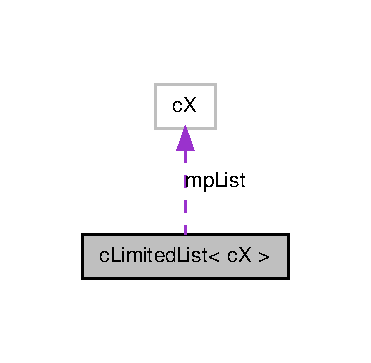
\includegraphics[width=178pt]{classc_limited_list__coll__graph}
\end{center}
\end{figure}
\subsection*{Public Member Functions}
\begin{DoxyCompactItemize}
\item 
void \hyperlink{classc_limited_list_ad909f4fc3256bfa9bc83b9baef8cac80}{ChangeSize} (uint32 liSize)
\item 
\hyperlink{classc_limited_list_a56cdd868a5924449791625ed2e462b03}{cLimitedList} ()
\item 
void \hyperlink{classc_limited_list_a29c4134a24a54d2d57498bb67447446e}{Init} (uint32 liSpaces)
\item 
\hyperlink{classc_limited_list_ae7c757c09f497da319f989e2042d488f}{cLimitedList} (uint32 liSpaces)
\item 
\hyperlink{classc_limited_list_ab7b63990b25112ae8cbf877b4fce7eed}{$\sim$cLimitedList} ()
\item 
cX \& \hyperlink{classc_limited_list_ae11b7c0a82de56c938eaf6d814838048}{operator\mbox{[}$\,$\mbox{]}} (uint32 liItem)
\item 
\hyperlink{classc_limited_list}{cLimitedList}$<$ cX $>$ \& \hyperlink{classc_limited_list_af6efd3116def79b9ca62cccc7ded030f}{operator=} (\hyperlink{classc_limited_list}{cLimitedList}$<$ cX $>$ \&lpOther)
\item 
uint32 \hyperlink{classc_limited_list_a0109c9831d7bf20d5ba259fc188be714}{Items} ()
\item 
void \hyperlink{classc_limited_list_a8a01caffbb1d69abf97481f12e59768d}{SetItems} (uint32 liItems)
\item 
void \hyperlink{classc_limited_list_a71e9c546a89a1be5cd656cc1284b4475}{Add} (cX $\ast$lpTemp)
\item 
void \hyperlink{classc_limited_list_a944c6ae2b1e13a144cc384766f9c12ae}{Remove} (uint32 liPos)
\item 
void \hyperlink{classc_limited_list_a378286ba482d356510d9a7a7b00395d9}{SwitchItems} (uint32 li1, uint32 li2)
\end{DoxyCompactItemize}
\subsection*{Public Attributes}
\begin{DoxyCompactItemize}
\item 
cX $\ast$ \hyperlink{classc_limited_list_aa3b0a10ecf4169b9bd7b41b0152e6a6a}{mpList}
\item 
uint32 \hyperlink{classc_limited_list_add31decc488d48f0037fe57a56c9aa4a}{miSpaces}
\item 
uint32 \hyperlink{classc_limited_list_a9509f6f3a5d9ad28608fbf288e43cf37}{miItems}
\end{DoxyCompactItemize}


\subsection{Detailed Description}
\subsubsection*{template$<$class cX$>$ class cLimitedList$<$ cX $>$}



Definition at line 5 of file WTLimitedList.h.



\subsection{Constructor \& Destructor Documentation}
\hypertarget{classc_limited_list_a56cdd868a5924449791625ed2e462b03}{
\index{cLimitedList@{cLimitedList}!cLimitedList@{cLimitedList}}
\index{cLimitedList@{cLimitedList}!cLimitedList@{cLimitedList}}
\subsubsection[{cLimitedList}]{\setlength{\rightskip}{0pt plus 5cm}template$<$class cX$>$ {\bf cLimitedList}$<$ cX $>$::{\bf cLimitedList} (
\begin{DoxyParamCaption}
{}
\end{DoxyParamCaption}
)\hspace{0.3cm}{\ttfamily  \mbox{[}inline\mbox{]}}}}
\label{classc_limited_list_a56cdd868a5924449791625ed2e462b03}


Definition at line 29 of file WTLimitedList.h.

\hypertarget{classc_limited_list_ae7c757c09f497da319f989e2042d488f}{
\index{cLimitedList@{cLimitedList}!cLimitedList@{cLimitedList}}
\index{cLimitedList@{cLimitedList}!cLimitedList@{cLimitedList}}
\subsubsection[{cLimitedList}]{\setlength{\rightskip}{0pt plus 5cm}template$<$class cX$>$ {\bf cLimitedList}$<$ cX $>$::{\bf cLimitedList} (
\begin{DoxyParamCaption}
\item[{uint32}]{liSpaces}
\end{DoxyParamCaption}
)\hspace{0.3cm}{\ttfamily  \mbox{[}inline\mbox{]}}}}
\label{classc_limited_list_ae7c757c09f497da319f989e2042d488f}


Definition at line 43 of file WTLimitedList.h.

\hypertarget{classc_limited_list_ab7b63990b25112ae8cbf877b4fce7eed}{
\index{cLimitedList@{cLimitedList}!$\sim$cLimitedList@{$\sim$cLimitedList}}
\index{$\sim$cLimitedList@{$\sim$cLimitedList}!cLimitedList@{cLimitedList}}
\subsubsection[{$\sim$cLimitedList}]{\setlength{\rightskip}{0pt plus 5cm}template$<$class cX$>$ {\bf cLimitedList}$<$ cX $>$::$\sim${\bf cLimitedList} (
\begin{DoxyParamCaption}
{}
\end{DoxyParamCaption}
)\hspace{0.3cm}{\ttfamily  \mbox{[}inline\mbox{]}}}}
\label{classc_limited_list_ab7b63990b25112ae8cbf877b4fce7eed}


Definition at line 48 of file WTLimitedList.h.



\subsection{Member Function Documentation}
\hypertarget{classc_limited_list_a71e9c546a89a1be5cd656cc1284b4475}{
\index{cLimitedList@{cLimitedList}!Add@{Add}}
\index{Add@{Add}!cLimitedList@{cLimitedList}}
\subsubsection[{Add}]{\setlength{\rightskip}{0pt plus 5cm}template$<$class cX$>$ void {\bf cLimitedList}$<$ cX $>$::Add (
\begin{DoxyParamCaption}
\item[{cX $\ast$}]{lpTemp}
\end{DoxyParamCaption}
)\hspace{0.3cm}{\ttfamily  \mbox{[}inline\mbox{]}}}}
\label{classc_limited_list_a71e9c546a89a1be5cd656cc1284b4475}


Definition at line 74 of file WTLimitedList.h.

\hypertarget{classc_limited_list_ad909f4fc3256bfa9bc83b9baef8cac80}{
\index{cLimitedList@{cLimitedList}!ChangeSize@{ChangeSize}}
\index{ChangeSize@{ChangeSize}!cLimitedList@{cLimitedList}}
\subsubsection[{ChangeSize}]{\setlength{\rightskip}{0pt plus 5cm}template$<$class cX$>$ void {\bf cLimitedList}$<$ cX $>$::ChangeSize (
\begin{DoxyParamCaption}
\item[{uint32}]{liSize}
\end{DoxyParamCaption}
)\hspace{0.3cm}{\ttfamily  \mbox{[}inline\mbox{]}}}}
\label{classc_limited_list_ad909f4fc3256bfa9bc83b9baef8cac80}


Definition at line 15 of file WTLimitedList.h.

\hypertarget{classc_limited_list_a29c4134a24a54d2d57498bb67447446e}{
\index{cLimitedList@{cLimitedList}!Init@{Init}}
\index{Init@{Init}!cLimitedList@{cLimitedList}}
\subsubsection[{Init}]{\setlength{\rightskip}{0pt plus 5cm}template$<$class cX$>$ void {\bf cLimitedList}$<$ cX $>$::Init (
\begin{DoxyParamCaption}
\item[{uint32}]{liSpaces}
\end{DoxyParamCaption}
)\hspace{0.3cm}{\ttfamily  \mbox{[}inline\mbox{]}}}}
\label{classc_limited_list_a29c4134a24a54d2d57498bb67447446e}


Definition at line 31 of file WTLimitedList.h.

\hypertarget{classc_limited_list_a0109c9831d7bf20d5ba259fc188be714}{
\index{cLimitedList@{cLimitedList}!Items@{Items}}
\index{Items@{Items}!cLimitedList@{cLimitedList}}
\subsubsection[{Items}]{\setlength{\rightskip}{0pt plus 5cm}template$<$class cX$>$ uint32 {\bf cLimitedList}$<$ cX $>$::Items (
\begin{DoxyParamCaption}
{}
\end{DoxyParamCaption}
)\hspace{0.3cm}{\ttfamily  \mbox{[}inline\mbox{]}}}}
\label{classc_limited_list_a0109c9831d7bf20d5ba259fc188be714}


Definition at line 71 of file WTLimitedList.h.

\hypertarget{classc_limited_list_af6efd3116def79b9ca62cccc7ded030f}{
\index{cLimitedList@{cLimitedList}!operator=@{operator=}}
\index{operator=@{operator=}!cLimitedList@{cLimitedList}}
\subsubsection[{operator=}]{\setlength{\rightskip}{0pt plus 5cm}template$<$class cX$>$ {\bf cLimitedList}$<$cX$>$\& {\bf cLimitedList}$<$ cX $>$::operator= (
\begin{DoxyParamCaption}
\item[{{\bf cLimitedList}$<$ cX $>$ \&}]{lpOther}
\end{DoxyParamCaption}
)\hspace{0.3cm}{\ttfamily  \mbox{[}inline\mbox{]}}}}
\label{classc_limited_list_af6efd3116def79b9ca62cccc7ded030f}


Definition at line 57 of file WTLimitedList.h.

\hypertarget{classc_limited_list_ae11b7c0a82de56c938eaf6d814838048}{
\index{cLimitedList@{cLimitedList}!operator\mbox{[}\mbox{]}@{operator[]}}
\index{operator\mbox{[}\mbox{]}@{operator[]}!cLimitedList@{cLimitedList}}
\subsubsection[{operator[]}]{\setlength{\rightskip}{0pt plus 5cm}template$<$class cX$>$ cX\& {\bf cLimitedList}$<$ cX $>$::operator\mbox{[}$\,$\mbox{]} (
\begin{DoxyParamCaption}
\item[{uint32}]{liItem}
\end{DoxyParamCaption}
)\hspace{0.3cm}{\ttfamily  \mbox{[}inline\mbox{]}}}}
\label{classc_limited_list_ae11b7c0a82de56c938eaf6d814838048}


Definition at line 55 of file WTLimitedList.h.

\hypertarget{classc_limited_list_a944c6ae2b1e13a144cc384766f9c12ae}{
\index{cLimitedList@{cLimitedList}!Remove@{Remove}}
\index{Remove@{Remove}!cLimitedList@{cLimitedList}}
\subsubsection[{Remove}]{\setlength{\rightskip}{0pt plus 5cm}template$<$class cX$>$ void {\bf cLimitedList}$<$ cX $>$::Remove (
\begin{DoxyParamCaption}
\item[{uint32}]{liPos}
\end{DoxyParamCaption}
)\hspace{0.3cm}{\ttfamily  \mbox{[}inline\mbox{]}}}}
\label{classc_limited_list_a944c6ae2b1e13a144cc384766f9c12ae}


Definition at line 76 of file WTLimitedList.h.

\hypertarget{classc_limited_list_a8a01caffbb1d69abf97481f12e59768d}{
\index{cLimitedList@{cLimitedList}!SetItems@{SetItems}}
\index{SetItems@{SetItems}!cLimitedList@{cLimitedList}}
\subsubsection[{SetItems}]{\setlength{\rightskip}{0pt plus 5cm}template$<$class cX$>$ void {\bf cLimitedList}$<$ cX $>$::SetItems (
\begin{DoxyParamCaption}
\item[{uint32}]{liItems}
\end{DoxyParamCaption}
)\hspace{0.3cm}{\ttfamily  \mbox{[}inline\mbox{]}}}}
\label{classc_limited_list_a8a01caffbb1d69abf97481f12e59768d}


Definition at line 72 of file WTLimitedList.h.

\hypertarget{classc_limited_list_a378286ba482d356510d9a7a7b00395d9}{
\index{cLimitedList@{cLimitedList}!SwitchItems@{SwitchItems}}
\index{SwitchItems@{SwitchItems}!cLimitedList@{cLimitedList}}
\subsubsection[{SwitchItems}]{\setlength{\rightskip}{0pt plus 5cm}template$<$class cX$>$ void {\bf cLimitedList}$<$ cX $>$::SwitchItems (
\begin{DoxyParamCaption}
\item[{uint32}]{li1, }
\item[{uint32}]{li2}
\end{DoxyParamCaption}
)\hspace{0.3cm}{\ttfamily  \mbox{[}inline\mbox{]}}}}
\label{classc_limited_list_a378286ba482d356510d9a7a7b00395d9}


Definition at line 86 of file WTLimitedList.h.



\subsection{Member Data Documentation}
\hypertarget{classc_limited_list_a9509f6f3a5d9ad28608fbf288e43cf37}{
\index{cLimitedList@{cLimitedList}!miItems@{miItems}}
\index{miItems@{miItems}!cLimitedList@{cLimitedList}}
\subsubsection[{miItems}]{\setlength{\rightskip}{0pt plus 5cm}template$<$class cX$>$ uint32 {\bf cLimitedList}$<$ cX $>$::{\bf miItems}}}
\label{classc_limited_list_a9509f6f3a5d9ad28608fbf288e43cf37}


Definition at line 13 of file WTLimitedList.h.

\hypertarget{classc_limited_list_add31decc488d48f0037fe57a56c9aa4a}{
\index{cLimitedList@{cLimitedList}!miSpaces@{miSpaces}}
\index{miSpaces@{miSpaces}!cLimitedList@{cLimitedList}}
\subsubsection[{miSpaces}]{\setlength{\rightskip}{0pt plus 5cm}template$<$class cX$>$ uint32 {\bf cLimitedList}$<$ cX $>$::{\bf miSpaces}}}
\label{classc_limited_list_add31decc488d48f0037fe57a56c9aa4a}


Definition at line 12 of file WTLimitedList.h.

\hypertarget{classc_limited_list_aa3b0a10ecf4169b9bd7b41b0152e6a6a}{
\index{cLimitedList@{cLimitedList}!mpList@{mpList}}
\index{mpList@{mpList}!cLimitedList@{cLimitedList}}
\subsubsection[{mpList}]{\setlength{\rightskip}{0pt plus 5cm}template$<$class cX$>$ cX$\ast$ {\bf cLimitedList}$<$ cX $>$::{\bf mpList}}}
\label{classc_limited_list_aa3b0a10ecf4169b9bd7b41b0152e6a6a}


Definition at line 11 of file WTLimitedList.h.


\hypertarget{classc_limited_pointer_list}{
\section{cLimitedPointerList$<$ cX $>$ Class Template Reference}
\label{classc_limited_pointer_list}\index{cLimitedPointerList@{cLimitedPointerList}}
}


This is similar to the \hyperlink{classc_limited_list}{cLimitedList} template class, but will uses pointers. The type cX is the base type. When a pointer is handed to the array, the list will store the pointer to the item and 'take ownership' of the object. This means that the item is NOT copied and when the list is deleted Items 'owned' to by the list will be deleted. This also makes array manipulation and size changing quicker. It will expand to accomodate new items added to the array.  


\subsection*{Public Member Functions}
\begin{DoxyCompactItemize}
\item 
\hypertarget{classc_limited_pointer_list_a07bb790fa0cce46a4724f87445278a2a}{
\hyperlink{classc_limited_pointer_list_a07bb790fa0cce46a4724f87445278a2a}{cLimitedPointerList} (uint32 liSpaces)}
\label{classc_limited_pointer_list_a07bb790fa0cce46a4724f87445278a2a}

\begin{DoxyCompactList}\small\item\em Constructor to create a new array of size liSpaces. \end{DoxyCompactList}\item 
\hypertarget{classc_limited_pointer_list_ad423e1b82ff902578d76e1e8ba33407f}{
\hyperlink{classc_limited_pointer_list_ad423e1b82ff902578d76e1e8ba33407f}{cLimitedPointerList} ()}
\label{classc_limited_pointer_list_ad423e1b82ff902578d76e1e8ba33407f}

\begin{DoxyCompactList}\small\item\em Constructor to create a 0 length array. \end{DoxyCompactList}\item 
\hypertarget{classc_limited_pointer_list_ab72b03a5d82ee318bf21d3102bdfecda}{
void \hyperlink{classc_limited_pointer_list_ab72b03a5d82ee318bf21d3102bdfecda}{Init} (uint32 liSpaces)}
\label{classc_limited_pointer_list_ab72b03a5d82ee318bf21d3102bdfecda}

\begin{DoxyCompactList}\small\item\em This will initialise the array to size liSpaces. \end{DoxyCompactList}\item 
\hypertarget{classc_limited_pointer_list_a7d77c2291a85cb39f06776e8d8555030}{
void \hyperlink{classc_limited_pointer_list_a7d77c2291a85cb39f06776e8d8555030}{ChangeSize} (uint32 liSize)}
\label{classc_limited_pointer_list_a7d77c2291a85cb39f06776e8d8555030}

\begin{DoxyCompactList}\small\item\em This will change the array size to liSize. Pointers will be copied across. If the new array is too short to store all the data. The excess objects will be deleted. \end{DoxyCompactList}\item 
\hypertarget{classc_limited_pointer_list_a5cd2eaf04fa51a23e35bb78ba875501f}{
void \hyperlink{classc_limited_pointer_list_a5cd2eaf04fa51a23e35bb78ba875501f}{DeleteAll} ()}
\label{classc_limited_pointer_list_a5cd2eaf04fa51a23e35bb78ba875501f}

\begin{DoxyCompactList}\small\item\em This will delete all items in the list. Clear the list to size 0. It will not delete this list object. \end{DoxyCompactList}\item 
\hypertarget{classc_limited_pointer_list_a4aef178a850d901cefc169cd0f8b1e71}{
\hyperlink{classc_limited_pointer_list_a4aef178a850d901cefc169cd0f8b1e71}{$\sim$cLimitedPointerList} ()}
\label{classc_limited_pointer_list_a4aef178a850d901cefc169cd0f8b1e71}

\begin{DoxyCompactList}\small\item\em Deconstructor for this list object. This will calll \hyperlink{classc_limited_pointer_list_a5cd2eaf04fa51a23e35bb78ba875501f}{DeleteAll()} \end{DoxyCompactList}\item 
\hypertarget{classc_limited_pointer_list_a118f2d5687c97cf122b163dbbdedb56d}{
cX $\ast$ \hyperlink{classc_limited_pointer_list_a118f2d5687c97cf122b163dbbdedb56d}{operator\mbox{[}$\,$\mbox{]}} (uint32 liItem)}
\label{classc_limited_pointer_list_a118f2d5687c97cf122b163dbbdedb56d}

\begin{DoxyCompactList}\small\item\em \mbox{[}\mbox{]} operatr to allow this to be used like a pointer array. \end{DoxyCompactList}\item 
\hypertarget{classc_limited_pointer_list_a00af27280f0a9d3f89fa8b9da36b7554}{
cX $\ast$ \hyperlink{classc_limited_pointer_list_a00af27280f0a9d3f89fa8b9da36b7554}{Item} (uint32 liItem)}
\label{classc_limited_pointer_list_a00af27280f0a9d3f89fa8b9da36b7554}

\begin{DoxyCompactList}\small\item\em Will return the pointer at position liItem in the list. \end{DoxyCompactList}\item 
\hypertarget{classc_limited_pointer_list_a0ba95ea83cbfee5957645c711ccab08c}{
void \hyperlink{classc_limited_pointer_list_a0ba95ea83cbfee5957645c711ccab08c}{Add} (cX $\ast$lpValue)}
\label{classc_limited_pointer_list_a0ba95ea83cbfee5957645c711ccab08c}

\begin{DoxyCompactList}\small\item\em Will Add the pointer lpValue to the list. Once added the Array will control deleting the object pointed to by lpValue. It will also expand the array to acomodate the item as required. \end{DoxyCompactList}\item 
\hypertarget{classc_limited_pointer_list_a61fdd759615a826b5f385ad0b9ddfb0d}{
void \hyperlink{classc_limited_pointer_list_a61fdd759615a826b5f385ad0b9ddfb0d}{Remove} (uint32 liPos)}
\label{classc_limited_pointer_list_a61fdd759615a826b5f385ad0b9ddfb0d}

\begin{DoxyCompactList}\small\item\em This will remove the item liPos from the List. It will delete the item and shuffle all the other items in teh list to the front of the list. \end{DoxyCompactList}\item 
\hypertarget{classc_limited_pointer_list_ad2981a22dcb5e79790b8644125cc7322}{
void \hyperlink{classc_limited_pointer_list_ad2981a22dcb5e79790b8644125cc7322}{SwitchItems} (uint32 li1, uint32 li2)}
\label{classc_limited_pointer_list_ad2981a22dcb5e79790b8644125cc7322}

\begin{DoxyCompactList}\small\item\em This will switch the positions of the items at positions li1 and li2 in the list. \end{DoxyCompactList}\end{DoxyCompactItemize}


\subsection{Detailed Description}
\subsubsection*{template$<$class cX$>$class cLimitedPointerList$<$ cX $>$}

This is similar to the \hyperlink{classc_limited_list}{cLimitedList} template class, but will uses pointers. The type cX is the base type. When a pointer is handed to the array, the list will store the pointer to the item and 'take ownership' of the object. This means that the item is NOT copied and when the list is deleted Items 'owned' to by the list will be deleted. This also makes array manipulation and size changing quicker. It will expand to accomodate new items added to the array. 
\hypertarget{classc_line}{
\section{cLine Class Reference}
\label{classc_line}\index{cLine@{cLine}}
}


A standard renderable Line object.  




Collaboration diagram for cLine:\nopagebreak
\begin{figure}[H]
\begin{center}
\leavevmode
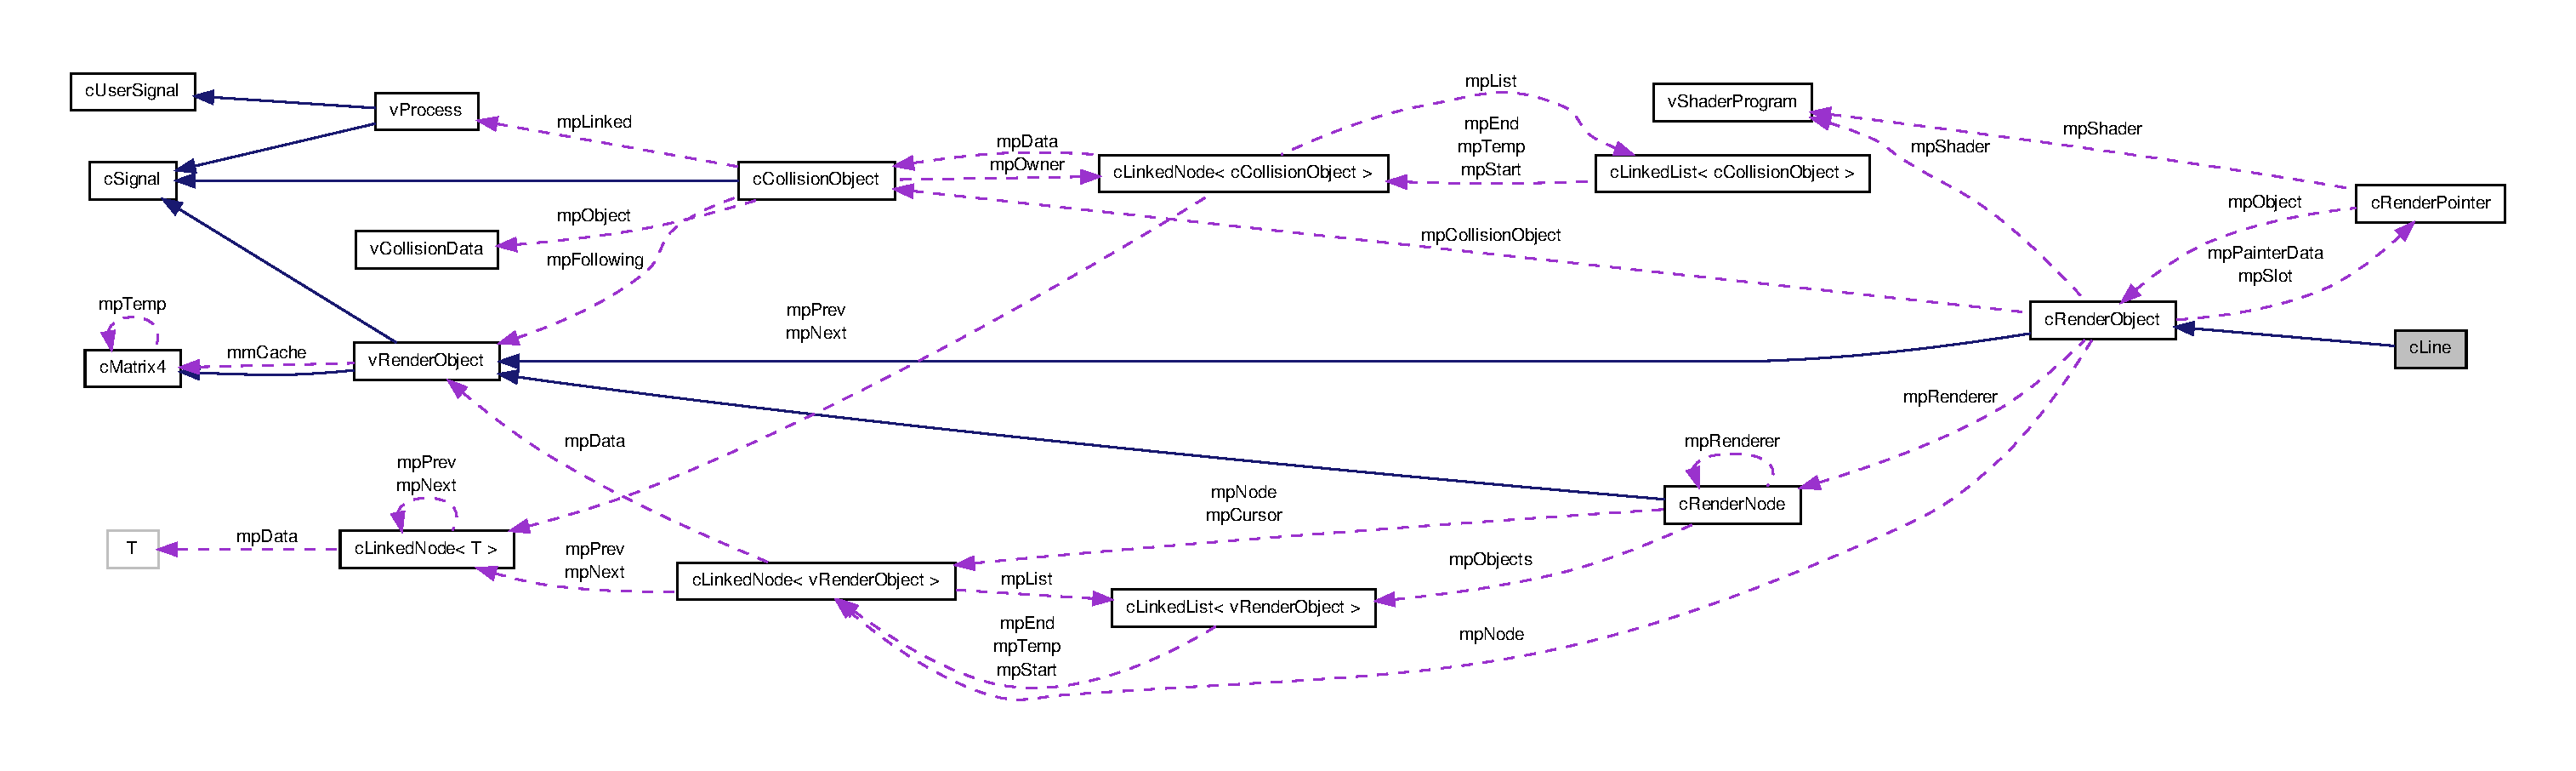
\includegraphics[height=600pt]{classc_line__coll__graph}
\end{center}
\end{figure}
\subsection*{Public Member Functions}
\begin{DoxyCompactItemize}
\item 
\hypertarget{classc_line_afc96602bef17f3d03af9685532af395d}{
\hyperlink{classc_line_afc96602bef17f3d03af9685532af395d}{cLine} ()}
\label{classc_line_afc96602bef17f3d03af9685532af395d}

\begin{DoxyCompactList}\small\item\em \hyperlink{classc_line}{cLine} constructor \end{DoxyCompactList}\item 
\hypertarget{classc_line_aa9c1d8af366fbcd7e5f71e82906a1b2c}{
\hyperlink{classc_line_aa9c1d8af366fbcd7e5f71e82906a1b2c}{cLine} (vRenderNode $\ast$lpRenderer)}
\label{classc_line_aa9c1d8af366fbcd7e5f71e82906a1b2c}

\begin{DoxyCompactList}\small\item\em \hyperlink{classc_line}{cLine} constructor. Will be owned by lpRenderer. \end{DoxyCompactList}\item 
\hypertarget{classc_line_a8a84cc1fe6a5a875faece391612347fc}{
\hyperlink{classc_line_a8a84cc1fe6a5a875faece391612347fc}{cLine} (\hyperlink{classc_camera}{cCamera} $\ast$lpCamera)}
\label{classc_line_a8a84cc1fe6a5a875faece391612347fc}

\begin{DoxyCompactList}\small\item\em \hyperlink{classc_line}{cLine} constructor. Will be owned by the \hyperlink{classc_render_node}{cRenderNode} of the \hyperlink{classc_camera}{cCamera} lpCamera. \end{DoxyCompactList}\item 
\hypertarget{classc_line_a32342ae3b470044b21f38f3fe3e0c232}{
float $\ast$ \hyperlink{classc_line_a32342ae3b470044b21f38f3fe3e0c232}{Position} ()}
\label{classc_line_a32342ae3b470044b21f38f3fe3e0c232}

\begin{DoxyCompactList}\small\item\em Will return a pointer to the position of this line object (XYZ). \end{DoxyCompactList}\item 
\hypertarget{classc_line_acfefe5128253475e8291d110f004095b}{
void \hyperlink{classc_line_acfefe5128253475e8291d110f004095b}{Position} (float $\ast$lfPos)}
\label{classc_line_acfefe5128253475e8291d110f004095b}

\begin{DoxyCompactList}\small\item\em Will set the position of this object to the float array pointed to by lfPos. Expects 3 floats (XYZ). \end{DoxyCompactList}\item 
\hypertarget{classc_line_aedeac0c1874b8212e8cc878b920513d9}{
void \hyperlink{classc_line_aedeac0c1874b8212e8cc878b920513d9}{Position} (float lfX, float lfY, float lfZ=0.0f)}
\label{classc_line_aedeac0c1874b8212e8cc878b920513d9}

\begin{DoxyCompactList}\small\item\em Will set the position of this object to the values specified (XYZ). \end{DoxyCompactList}\item 
\hypertarget{classc_line_a4b37bd0ff6ea3834a2c49d5efbd222c9}{
float $\ast$ \hyperlink{classc_line_a4b37bd0ff6ea3834a2c49d5efbd222c9}{Vector} ()}
\label{classc_line_a4b37bd0ff6ea3834a2c49d5efbd222c9}

\begin{DoxyCompactList}\small\item\em Will return a pointer to the vector of this line object (XYZ). \end{DoxyCompactList}\item 
\hypertarget{classc_line_ad558bfa28a78a6594446ae0c5e11c262}{
void \hyperlink{classc_line_ad558bfa28a78a6594446ae0c5e11c262}{Vector} (float $\ast$lfPos)}
\label{classc_line_ad558bfa28a78a6594446ae0c5e11c262}

\begin{DoxyCompactList}\small\item\em Will set the vector of this object to the float array pointed to by lfPos. Expects 3 floats (XYZ). \end{DoxyCompactList}\item 
\hypertarget{classc_line_abfbbb77ed5b1c9208baf6d38b907b7b5}{
void \hyperlink{classc_line_abfbbb77ed5b1c9208baf6d38b907b7b5}{Vector} (float lfX, float lfY, float lfZ=0.0f)}
\label{classc_line_abfbbb77ed5b1c9208baf6d38b907b7b5}

\begin{DoxyCompactList}\small\item\em Will set the vector of this object to the values specified (XYZ). \end{DoxyCompactList}\item 
\hypertarget{classc_line_a4b02fb7febded866cc8fda351d623811}{
void \hyperlink{classc_line_a4b02fb7febded866cc8fda351d623811}{Width} (float lfWidth)}
\label{classc_line_a4b02fb7febded866cc8fda351d623811}

\begin{DoxyCompactList}\small\item\em Will set the width for the line. \end{DoxyCompactList}\item 
\hypertarget{classc_line_a26247a346a469646b250fa0116e1ec34}{
float \hyperlink{classc_line_a26247a346a469646b250fa0116e1ec34}{Width} ()}
\label{classc_line_a26247a346a469646b250fa0116e1ec34}

\begin{DoxyCompactList}\small\item\em Will return the lines width. \end{DoxyCompactList}\end{DoxyCompactItemize}


\subsection{Detailed Description}
A standard renderable Line object. 
\hypertarget{classc_linked_list}{
\section{cLinkedList$<$ T $>$ Class Template Reference}
\label{classc_linked_list}\index{cLinkedList@{cLinkedList}}
}


This is the control for a linked list. It controls a linked list of cLinkedNodes which each point to their item in the list. Each \hyperlink{classc_linked_node}{cLinkedNode} poitns to the \hyperlink{classc_linked_node}{cLinkedNode} s either side of themselves and the data they own. \hyperlink{classc_linked_list}{cLinkedList} is templated and so can be a linked list of any type.  


\subsection*{Public Member Functions}
\begin{DoxyCompactItemize}
\item 
void \hyperlink{classc_linked_list_a57cda13916eac63747ff70071907d7ca}{StitchOut} (\hyperlink{classc_linked_node}{cLinkedNode}$<$ T $>$ $\ast$lpNode)
\item 
void \hyperlink{classc_linked_list_adf5505edbd4933ccde08183c539e6655}{StitchIn} (\hyperlink{classc_linked_node}{cLinkedNode}$<$ T $>$ $\ast$lpNode)
\item 
void \hyperlink{classc_linked_list_acdd0ec24de3bc0a706e1ec8b4a2cb2ae}{StitchIn} (\hyperlink{classc_linked_node}{cLinkedNode}$<$ T $>$ $\ast$lpNode, \hyperlink{classc_linked_node}{cLinkedNode}$<$ T $>$ $\ast$lpPos)
\item 
\hyperlink{classc_linked_list_adbdde7829ddb9dc0518126d8e0164e10}{cLinkedList} (T $\ast$lpData)
\begin{DoxyCompactList}\small\item\em This holds a pointer of the relevant type for the list and will create the list by making the item lpData the first item in the list. \item\end{DoxyCompactList}\item 
\hyperlink{classc_linked_list_a2aacceb9a6498158af9598cb424977e3}{cLinkedList} ()
\item 
\hyperlink{classc_linked_list_a80aef75883bffae5da5ee7d8b9258502}{$\sim$cLinkedList} ()
\begin{DoxyCompactList}\small\item\em This will delete the list and delete every item in the list. \item\end{DoxyCompactList}\item 
\hyperlink{classc_linked_node}{cLinkedNode}$<$ T $>$ $\ast$ \hyperlink{classc_linked_list_a91593c408e5c5fc719624531f996c29c}{Start} ()
\item 
\hyperlink{classc_linked_node}{cLinkedNode}$<$ T $>$ $\ast$ \hyperlink{classc_linked_list_a95267afd7cde82576255fbde914a7e0d}{End} ()
\item 
\hyperlink{classc_linked_node}{cLinkedNode}$<$ T $>$ $\ast$ \hyperlink{classc_linked_list_a6014141bbd16b32e22b4b7deb873f1ae}{Find} (T $\ast$lpData)
\begin{DoxyCompactList}\small\item\em This is the number of items in the list. \item\end{DoxyCompactList}\item 
\hyperlink{classc_linked_node}{cLinkedNode}$<$ T $>$ $\ast$ \hyperlink{classc_linked_list_ae9bedf047bccf0f63b10b662c809032c}{Insert} (T $\ast$lpData)
\begin{DoxyCompactList}\small\item\em This will create a \hyperlink{classc_linked_node}{cLinkedNode} give it lpData and add that node to the end of the list. \item\end{DoxyCompactList}\item 
void \hyperlink{classc_linked_list_ab4694aa48324f52b8b1c25eb43dc996c}{Delete} (\hyperlink{classc_linked_node}{cLinkedNode}$<$ T $>$ $\ast$lpOld)
\begin{DoxyCompactList}\small\item\em This will delete the \hyperlink{classc_linked_node}{cLinkedNode} pointed to by lpOld and remove it from the list including mpData. \item\end{DoxyCompactList}\item 
void \hyperlink{classc_linked_list_a1806f7d9fcba9d78f54b2787919d5407}{Initialise} ()
\item 
void \hyperlink{classc_linked_list_a4f6cff87d2c90874949757987f6b9748}{Move} (\hyperlink{classc_linked_node}{cLinkedNode}$<$ T $>$ $\ast$lpFrom, \hyperlink{classc_linked_node}{cLinkedNode}$<$ T $>$ $\ast$lpPosition)
\begin{DoxyCompactList}\small\item\em This will Move the node lpFrom to be before lpPosition. \item\end{DoxyCompactList}\item 
void \hyperlink{classc_linked_list_ad62406784a55a3477383c51a59ec7603}{Move} (\hyperlink{classc_linked_node}{cLinkedNode}$<$ T $>$ $\ast$lpFrom, \hyperlink{classc_linked_list}{cLinkedList}$<$ T $>$ $\ast$lpPosition)
\item 
void \hyperlink{classc_linked_list_a48b99bef680a675623c84684c17691a6}{ClearAll} ()
\item 
void \hyperlink{classc_linked_list_a6116806e9435ffde67f1c26f1138e431}{DeleteAll} ()
\item 
void \hyperlink{classc_linked_list_a476170cb815fe62c516fc3fb439d9c19}{Display} ()
\item 
void \hyperlink{classc_linked_list_a676cd3bd124df98773c296ed6f67ba16}{Remove} (\hyperlink{classc_linked_node}{cLinkedNode}$<$ T $>$ $\ast$lpNode)
\begin{DoxyCompactList}\small\item\em This will delete the \hyperlink{classc_linked_node}{cLinkedNode} pointed to by lpOld and remove it from the list, but not delete mpData. \item\end{DoxyCompactList}\end{DoxyCompactItemize}
\subsection*{Static Public Attributes}
\begin{DoxyCompactItemize}
\item 
static \hyperlink{classc_linked_node}{cLinkedNode}$<$ T $>$ $\ast$ \hyperlink{classc_linked_list_abc440dbcbff9bcfb6e538a0e008c27c1}{mpTemp} = 0
\begin{DoxyCompactList}\small\item\em This is a pointer that can be used as a cursor by this linked list. \item\end{DoxyCompactList}\end{DoxyCompactItemize}


\subsection{Detailed Description}
\subsubsection*{template$<$class T$>$ class cLinkedList$<$ T $>$}

This is the control for a linked list. It controls a linked list of cLinkedNodes which each point to their item in the list. Each \hyperlink{classc_linked_node}{cLinkedNode} poitns to the \hyperlink{classc_linked_node}{cLinkedNode} s either side of themselves and the data they own. \hyperlink{classc_linked_list}{cLinkedList} is templated and so can be a linked list of any type. 

Definition at line 50 of file WTLLTemplate.h.



\subsection{Constructor \& Destructor Documentation}
\hypertarget{classc_linked_list_adbdde7829ddb9dc0518126d8e0164e10}{
\index{cLinkedList@{cLinkedList}!cLinkedList@{cLinkedList}}
\index{cLinkedList@{cLinkedList}!cLinkedList@{cLinkedList}}
\subsubsection[{cLinkedList}]{\setlength{\rightskip}{0pt plus 5cm}template$<$class T$>$ {\bf cLinkedList}$<$ T $>$::{\bf cLinkedList} (
\begin{DoxyParamCaption}
\item[{T $\ast$}]{lpData}
\end{DoxyParamCaption}
)}}
\label{classc_linked_list_adbdde7829ddb9dc0518126d8e0164e10}


This holds a pointer of the relevant type for the list and will create the list by making the item lpData the first item in the list. 



Definition at line 276 of file WTLLTemplate.h.

\hypertarget{classc_linked_list_a2aacceb9a6498158af9598cb424977e3}{
\index{cLinkedList@{cLinkedList}!cLinkedList@{cLinkedList}}
\index{cLinkedList@{cLinkedList}!cLinkedList@{cLinkedList}}
\subsubsection[{cLinkedList}]{\setlength{\rightskip}{0pt plus 5cm}template$<$class T$>$ {\bf cLinkedList}$<$ T $>$::{\bf cLinkedList} (
\begin{DoxyParamCaption}
{}
\end{DoxyParamCaption}
)}}
\label{classc_linked_list_a2aacceb9a6498158af9598cb424977e3}


Definition at line 183 of file WTLLTemplate.h.

\hypertarget{classc_linked_list_a80aef75883bffae5da5ee7d8b9258502}{
\index{cLinkedList@{cLinkedList}!$\sim$cLinkedList@{$\sim$cLinkedList}}
\index{$\sim$cLinkedList@{$\sim$cLinkedList}!cLinkedList@{cLinkedList}}
\subsubsection[{$\sim$cLinkedList}]{\setlength{\rightskip}{0pt plus 5cm}template$<$class T$>$ {\bf cLinkedList}$<$ T $>$::$\sim${\bf cLinkedList} (
\begin{DoxyParamCaption}
{}
\end{DoxyParamCaption}
)\hspace{0.3cm}{\ttfamily  \mbox{[}inline\mbox{]}}}}
\label{classc_linked_list_a80aef75883bffae5da5ee7d8b9258502}


This will delete the list and delete every item in the list. 



Definition at line 68 of file WTLLTemplate.h.



\subsection{Member Function Documentation}
\hypertarget{classc_linked_list_a48b99bef680a675623c84684c17691a6}{
\index{cLinkedList@{cLinkedList}!ClearAll@{ClearAll}}
\index{ClearAll@{ClearAll}!cLinkedList@{cLinkedList}}
\subsubsection[{ClearAll}]{\setlength{\rightskip}{0pt plus 5cm}template$<$class T $>$ void {\bf cLinkedList}$<$ T $>$::ClearAll (
\begin{DoxyParamCaption}
{}
\end{DoxyParamCaption}
)}}
\label{classc_linked_list_a48b99bef680a675623c84684c17691a6}


Definition at line 189 of file WTLLTemplate.h.

\hypertarget{classc_linked_list_ab4694aa48324f52b8b1c25eb43dc996c}{
\index{cLinkedList@{cLinkedList}!Delete@{Delete}}
\index{Delete@{Delete}!cLinkedList@{cLinkedList}}
\subsubsection[{Delete}]{\setlength{\rightskip}{0pt plus 5cm}template$<$class T$>$ void {\bf cLinkedList}$<$ T $>$::Delete (
\begin{DoxyParamCaption}
\item[{{\bf cLinkedNode}$<$ T $>$ $\ast$}]{lpOld}
\end{DoxyParamCaption}
)}}
\label{classc_linked_list_ab4694aa48324f52b8b1c25eb43dc996c}


This will delete the \hyperlink{classc_linked_node}{cLinkedNode} pointed to by lpOld and remove it from the list including mpData. 



Definition at line 226 of file WTLLTemplate.h.

\hypertarget{classc_linked_list_a6116806e9435ffde67f1c26f1138e431}{
\index{cLinkedList@{cLinkedList}!DeleteAll@{DeleteAll}}
\index{DeleteAll@{DeleteAll}!cLinkedList@{cLinkedList}}
\subsubsection[{DeleteAll}]{\setlength{\rightskip}{0pt plus 5cm}template$<$class T $>$ void {\bf cLinkedList}$<$ T $>$::DeleteAll (
\begin{DoxyParamCaption}
{}
\end{DoxyParamCaption}
)}}
\label{classc_linked_list_a6116806e9435ffde67f1c26f1138e431}


Definition at line 116 of file WTLLTemplate.h.

\hypertarget{classc_linked_list_a476170cb815fe62c516fc3fb439d9c19}{
\index{cLinkedList@{cLinkedList}!Display@{Display}}
\index{Display@{Display}!cLinkedList@{cLinkedList}}
\subsubsection[{Display}]{\setlength{\rightskip}{0pt plus 5cm}template$<$class T $>$ void {\bf cLinkedList}$<$ T $>$::Display (
\begin{DoxyParamCaption}
{}
\end{DoxyParamCaption}
)}}
\label{classc_linked_list_a476170cb815fe62c516fc3fb439d9c19}


Definition at line 300 of file WTLLTemplate.h.

\hypertarget{classc_linked_list_a95267afd7cde82576255fbde914a7e0d}{
\index{cLinkedList@{cLinkedList}!End@{End}}
\index{End@{End}!cLinkedList@{cLinkedList}}
\subsubsection[{End}]{\setlength{\rightskip}{0pt plus 5cm}template$<$class T$>$ {\bf cLinkedNode}$<$T$>$$\ast$ {\bf cLinkedList}$<$ T $>$::End (
\begin{DoxyParamCaption}
{}
\end{DoxyParamCaption}
)\hspace{0.3cm}{\ttfamily  \mbox{[}inline\mbox{]}}}}
\label{classc_linked_list_a95267afd7cde82576255fbde914a7e0d}


Definition at line 75 of file WTLLTemplate.h.

\hypertarget{classc_linked_list_a6014141bbd16b32e22b4b7deb873f1ae}{
\index{cLinkedList@{cLinkedList}!Find@{Find}}
\index{Find@{Find}!cLinkedList@{cLinkedList}}
\subsubsection[{Find}]{\setlength{\rightskip}{0pt plus 5cm}template$<$class T$>$ {\bf cLinkedNode}$<$ T $>$ $\ast$ {\bf cLinkedList}$<$ T $>$::Find (
\begin{DoxyParamCaption}
\item[{T $\ast$}]{lpData}
\end{DoxyParamCaption}
)}}
\label{classc_linked_list_a6014141bbd16b32e22b4b7deb873f1ae}


This is the number of items in the list. 

This will return the \hyperlink{classc_linked_node}{cLinkedNode} which owns the item lpData in this list. 

Definition at line 219 of file WTLLTemplate.h.

\hypertarget{classc_linked_list_a1806f7d9fcba9d78f54b2787919d5407}{
\index{cLinkedList@{cLinkedList}!Initialise@{Initialise}}
\index{Initialise@{Initialise}!cLinkedList@{cLinkedList}}
\subsubsection[{Initialise}]{\setlength{\rightskip}{0pt plus 5cm}template$<$class T $>$ void {\bf cLinkedList}$<$ T $>$::Initialise (
\begin{DoxyParamCaption}
{}
\end{DoxyParamCaption}
)}}
\label{classc_linked_list_a1806f7d9fcba9d78f54b2787919d5407}


Definition at line 107 of file WTLLTemplate.h.

\hypertarget{classc_linked_list_ae9bedf047bccf0f63b10b662c809032c}{
\index{cLinkedList@{cLinkedList}!Insert@{Insert}}
\index{Insert@{Insert}!cLinkedList@{cLinkedList}}
\subsubsection[{Insert}]{\setlength{\rightskip}{0pt plus 5cm}template$<$class T$>$ {\bf cLinkedNode}$<$ T $>$ $\ast$ {\bf cLinkedList}$<$ T $>$::Insert (
\begin{DoxyParamCaption}
\item[{T $\ast$}]{lpData}
\end{DoxyParamCaption}
)}}
\label{classc_linked_list_ae9bedf047bccf0f63b10b662c809032c}


This will create a \hyperlink{classc_linked_node}{cLinkedNode} give it lpData and add that node to the end of the list. 



Definition at line 289 of file WTLLTemplate.h.

\hypertarget{classc_linked_list_a4f6cff87d2c90874949757987f6b9748}{
\index{cLinkedList@{cLinkedList}!Move@{Move}}
\index{Move@{Move}!cLinkedList@{cLinkedList}}
\subsubsection[{Move}]{\setlength{\rightskip}{0pt plus 5cm}template$<$class T$>$ void {\bf cLinkedList}$<$ T $>$::Move (
\begin{DoxyParamCaption}
\item[{{\bf cLinkedNode}$<$ T $>$ $\ast$}]{lpFrom, }
\item[{{\bf cLinkedNode}$<$ T $>$ $\ast$}]{lpPosition}
\end{DoxyParamCaption}
)}}
\label{classc_linked_list_a4f6cff87d2c90874949757987f6b9748}


This will Move the node lpFrom to be before lpPosition. 

\hypertarget{classc_linked_list_ad62406784a55a3477383c51a59ec7603}{
\index{cLinkedList@{cLinkedList}!Move@{Move}}
\index{Move@{Move}!cLinkedList@{cLinkedList}}
\subsubsection[{Move}]{\setlength{\rightskip}{0pt plus 5cm}template$<$class T$>$ void {\bf cLinkedList}$<$ T $>$::Move (
\begin{DoxyParamCaption}
\item[{{\bf cLinkedNode}$<$ T $>$ $\ast$}]{lpFrom, }
\item[{{\bf cLinkedList}$<$ T $>$ $\ast$}]{lpPosition}
\end{DoxyParamCaption}
)}}
\label{classc_linked_list_ad62406784a55a3477383c51a59ec7603}


Definition at line 208 of file WTLLTemplate.h.

\hypertarget{classc_linked_list_a676cd3bd124df98773c296ed6f67ba16}{
\index{cLinkedList@{cLinkedList}!Remove@{Remove}}
\index{Remove@{Remove}!cLinkedList@{cLinkedList}}
\subsubsection[{Remove}]{\setlength{\rightskip}{0pt plus 5cm}template$<$class T$>$ void {\bf cLinkedList}$<$ T $>$::Remove (
\begin{DoxyParamCaption}
\item[{{\bf cLinkedNode}$<$ T $>$ $\ast$}]{lpNode}
\end{DoxyParamCaption}
)}}
\label{classc_linked_list_a676cd3bd124df98773c296ed6f67ba16}


This will delete the \hyperlink{classc_linked_node}{cLinkedNode} pointed to by lpOld and remove it from the list, but not delete mpData. 



Definition at line 155 of file WTLLTemplate.h.

\hypertarget{classc_linked_list_a91593c408e5c5fc719624531f996c29c}{
\index{cLinkedList@{cLinkedList}!Start@{Start}}
\index{Start@{Start}!cLinkedList@{cLinkedList}}
\subsubsection[{Start}]{\setlength{\rightskip}{0pt plus 5cm}template$<$class T$>$ {\bf cLinkedNode}$<$T$>$$\ast$ {\bf cLinkedList}$<$ T $>$::Start (
\begin{DoxyParamCaption}
{}
\end{DoxyParamCaption}
)\hspace{0.3cm}{\ttfamily  \mbox{[}inline\mbox{]}}}}
\label{classc_linked_list_a91593c408e5c5fc719624531f996c29c}


Definition at line 73 of file WTLLTemplate.h.

\hypertarget{classc_linked_list_adf5505edbd4933ccde08183c539e6655}{
\index{cLinkedList@{cLinkedList}!StitchIn@{StitchIn}}
\index{StitchIn@{StitchIn}!cLinkedList@{cLinkedList}}
\subsubsection[{StitchIn}]{\setlength{\rightskip}{0pt plus 5cm}template$<$class T$>$ void {\bf cLinkedList}$<$ T $>$::StitchIn (
\begin{DoxyParamCaption}
\item[{{\bf cLinkedNode}$<$ T $>$ $\ast$}]{lpNode}
\end{DoxyParamCaption}
)}}
\label{classc_linked_list_adf5505edbd4933ccde08183c539e6655}


Definition at line 235 of file WTLLTemplate.h.

\hypertarget{classc_linked_list_acdd0ec24de3bc0a706e1ec8b4a2cb2ae}{
\index{cLinkedList@{cLinkedList}!StitchIn@{StitchIn}}
\index{StitchIn@{StitchIn}!cLinkedList@{cLinkedList}}
\subsubsection[{StitchIn}]{\setlength{\rightskip}{0pt plus 5cm}template$<$class T$>$ void {\bf cLinkedList}$<$ T $>$::StitchIn (
\begin{DoxyParamCaption}
\item[{{\bf cLinkedNode}$<$ T $>$ $\ast$}]{lpNode, }
\item[{{\bf cLinkedNode}$<$ T $>$ $\ast$}]{lpPos}
\end{DoxyParamCaption}
)}}
\label{classc_linked_list_acdd0ec24de3bc0a706e1ec8b4a2cb2ae}


Definition at line 255 of file WTLLTemplate.h.

\hypertarget{classc_linked_list_a57cda13916eac63747ff70071907d7ca}{
\index{cLinkedList@{cLinkedList}!StitchOut@{StitchOut}}
\index{StitchOut@{StitchOut}!cLinkedList@{cLinkedList}}
\subsubsection[{StitchOut}]{\setlength{\rightskip}{0pt plus 5cm}template$<$class T$>$ void {\bf cLinkedList}$<$ T $>$::StitchOut (
\begin{DoxyParamCaption}
\item[{{\bf cLinkedNode}$<$ T $>$ $\ast$}]{lpNode}
\end{DoxyParamCaption}
)}}
\label{classc_linked_list_a57cda13916eac63747ff70071907d7ca}


Definition at line 163 of file WTLLTemplate.h.



\subsection{Member Data Documentation}
\hypertarget{classc_linked_list_abc440dbcbff9bcfb6e538a0e008c27c1}{
\index{cLinkedList@{cLinkedList}!mpTemp@{mpTemp}}
\index{mpTemp@{mpTemp}!cLinkedList@{cLinkedList}}
\subsubsection[{mpTemp}]{\setlength{\rightskip}{0pt plus 5cm}template$<$class T$>$ {\bf cLinkedNode}$<$ T $>$ $\ast$ {\bf cLinkedList}$<$ T $>$::{\bf mpTemp} = 0\hspace{0.3cm}{\ttfamily  \mbox{[}static\mbox{]}}}}
\label{classc_linked_list_abc440dbcbff9bcfb6e538a0e008c27c1}


This is a pointer that can be used as a cursor by this linked list. 



Definition at line 75 of file WTLLTemplate.h.


\hypertarget{classc_linked_node}{
\section{cLinkedNode$<$ T $>$ Class Template Reference}
\label{classc_linked_node}\index{cLinkedNode@{cLinkedNode}}
}


This is a node class to allow templating of the \hyperlink{classc_linked_list}{cLinkedList} class. This node will store pointers to the nodes either side of this node in the linked list and a pointer to the object his node owns.  




Collaboration diagram for cLinkedNode$<$ T $>$:\nopagebreak
\begin{figure}[H]
\begin{center}
\leavevmode
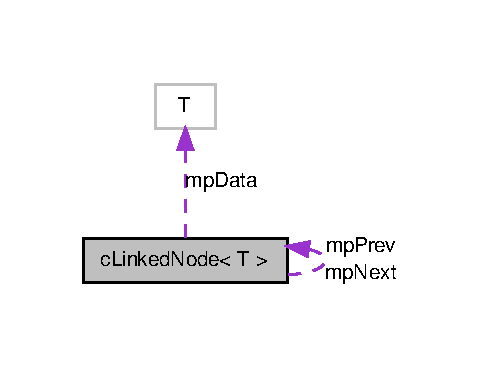
\includegraphics[width=231pt]{classc_linked_node__coll__graph}
\end{center}
\end{figure}
\subsection*{Public Member Functions}
\begin{DoxyCompactItemize}
\item 
\hypertarget{classc_linked_node_adb8af44378d6d47b439ec7950f579bb3}{
\hyperlink{classc_linked_node_adb8af44378d6d47b439ec7950f579bb3}{$\sim$cLinkedNode} ()}
\label{classc_linked_node_adb8af44378d6d47b439ec7950f579bb3}

\begin{DoxyCompactList}\small\item\em This will delete the data owned by this node as it is deconstructed. \end{DoxyCompactList}\item 
\hypertarget{classc_linked_node_ac375aeade4f13f07a601732e80b49e8b}{
\hyperlink{classc_linked_node}{cLinkedNode}$<$ T $>$ $\ast$ \hyperlink{classc_linked_node_ac375aeade4f13f07a601732e80b49e8b}{Next} ()}
\label{classc_linked_node_ac375aeade4f13f07a601732e80b49e8b}

\begin{DoxyCompactList}\small\item\em This will return a pointer to the next node in the linked list. see \hyperlink{classc_linked_list}{cLinkedList}. \end{DoxyCompactList}\item 
\hypertarget{classc_linked_node_a6481dec71a6adffa72fd9621f366253a}{
\hyperlink{classc_linked_node}{cLinkedNode}$<$ T $>$ $\ast$ \hyperlink{classc_linked_node_a6481dec71a6adffa72fd9621f366253a}{Previous} ()}
\label{classc_linked_node_a6481dec71a6adffa72fd9621f366253a}

\begin{DoxyCompactList}\small\item\em This will return a pointer to the previous node in the linked list. see \hyperlink{classc_linked_list}{cLinkedList}. \end{DoxyCompactList}\end{DoxyCompactItemize}
\subsection*{Friends}
\begin{DoxyCompactItemize}
\item 
\hypertarget{classc_linked_node_a5b538a518f67ed3377a26348f2b536da}{
class \hyperlink{classc_linked_node_a5b538a518f67ed3377a26348f2b536da}{cLinkedList$<$ T $>$}}
\label{classc_linked_node_a5b538a518f67ed3377a26348f2b536da}

\end{DoxyCompactItemize}


\subsection{Detailed Description}
\subsubsection*{template$<$class T$>$class cLinkedNode$<$ T $>$}

This is a node class to allow templating of the \hyperlink{classc_linked_list}{cLinkedList} class. This node will store pointers to the nodes either side of this node in the linked list and a pointer to the object his node owns. 
\hypertarget{classc_main_thread}{
\section{cMainThread$<$ cX, cS $>$ Class Template Reference}
\label{classc_main_thread}\index{cMainThread@{cMainThread}}
}
\subsection*{Public Member Functions}
\begin{DoxyCompactItemize}
\item 
\hyperlink{classc_main_thread_a6eb20e854fb31291be7cd3ca35a2c68c}{$\sim$cMainThread} ()
\item 
\hyperlink{classc_main_thread_a6eb20e854fb31291be7cd3ca35a2c68c}{$\sim$cMainThread} ()
\end{DoxyCompactItemize}
\subsection*{Static Public Member Functions}
\begin{DoxyCompactItemize}
\item 
static uint32 \hyperlink{classc_main_thread_a46319ac6fe2f17e5f8399e1a5ae04b2f}{Start} (HINSTANCE hInstance)
\item 
static uint32 \hyperlink{classc_main_thread_af7a34c0a224a60eb9f1273b9f1e6ddcb}{Start} ()
\end{DoxyCompactItemize}


\subsection{Detailed Description}
\subsubsection*{template$<$class cX, class cS$>$ class cMainThread$<$ cX, cS $>$}



Definition at line 8 of file WTcBase.h.



\subsection{Constructor \& Destructor Documentation}
\hypertarget{classc_main_thread_a6eb20e854fb31291be7cd3ca35a2c68c}{
\index{cMainThread@{cMainThread}!$\sim$cMainThread@{$\sim$cMainThread}}
\index{$\sim$cMainThread@{$\sim$cMainThread}!cMainThread@{cMainThread}}
\subsubsection[{$\sim$cMainThread}]{\setlength{\rightskip}{0pt plus 5cm}template$<$class cX , class cS $>$ {\bf cMainThread}$<$ cX, cS $>$::$\sim${\bf cMainThread} (
\begin{DoxyParamCaption}
{}
\end{DoxyParamCaption}
)\hspace{0.3cm}{\ttfamily  \mbox{[}inline\mbox{]}}}}
\label{classc_main_thread_a6eb20e854fb31291be7cd3ca35a2c68c}


Definition at line 12 of file WTcBase.h.

\hypertarget{classc_main_thread_a6eb20e854fb31291be7cd3ca35a2c68c}{
\index{cMainThread@{cMainThread}!$\sim$cMainThread@{$\sim$cMainThread}}
\index{$\sim$cMainThread@{$\sim$cMainThread}!cMainThread@{cMainThread}}
\subsubsection[{$\sim$cMainThread}]{\setlength{\rightskip}{0pt plus 5cm}template$<$class cX , class cS $>$ {\bf cMainThread}$<$ cX, cS $>$::$\sim${\bf cMainThread} (
\begin{DoxyParamCaption}
{}
\end{DoxyParamCaption}
)\hspace{0.3cm}{\ttfamily  \mbox{[}inline\mbox{]}}}}
\label{classc_main_thread_a6eb20e854fb31291be7cd3ca35a2c68c}


Definition at line 51 of file WTcBase.h.



\subsection{Member Function Documentation}
\hypertarget{classc_main_thread_a46319ac6fe2f17e5f8399e1a5ae04b2f}{
\index{cMainThread@{cMainThread}!Start@{Start}}
\index{Start@{Start}!cMainThread@{cMainThread}}
\subsubsection[{Start}]{\setlength{\rightskip}{0pt plus 5cm}template$<$class cX , class cS $>$ static uint32 {\bf cMainThread}$<$ cX, cS $>$::Start (
\begin{DoxyParamCaption}
\item[{HINSTANCE}]{hInstance}
\end{DoxyParamCaption}
)\hspace{0.3cm}{\ttfamily  \mbox{[}inline, static\mbox{]}}}}
\label{classc_main_thread_a46319ac6fe2f17e5f8399e1a5ae04b2f}


Definition at line 13 of file WTcBase.h.

\hypertarget{classc_main_thread_af7a34c0a224a60eb9f1273b9f1e6ddcb}{
\index{cMainThread@{cMainThread}!Start@{Start}}
\index{Start@{Start}!cMainThread@{cMainThread}}
\subsubsection[{Start}]{\setlength{\rightskip}{0pt plus 5cm}template$<$class cX , class cS $>$ static uint32 {\bf cMainThread}$<$ cX, cS $>$::Start (
\begin{DoxyParamCaption}
{}
\end{DoxyParamCaption}
)\hspace{0.3cm}{\ttfamily  \mbox{[}inline, static\mbox{]}}}}
\label{classc_main_thread_af7a34c0a224a60eb9f1273b9f1e6ddcb}


Definition at line 52 of file WTcBase.h.


\hypertarget{classc_material}{
\section{cMaterial Class Reference}
\label{classc_material}\index{cMaterial@{cMaterial}}
}


A class to store material data for an object. Defines the 'reflectiveness' of the surface.  




Inheritance diagram for cMaterial:
\nopagebreak
\begin{figure}[H]
\begin{center}
\leavevmode
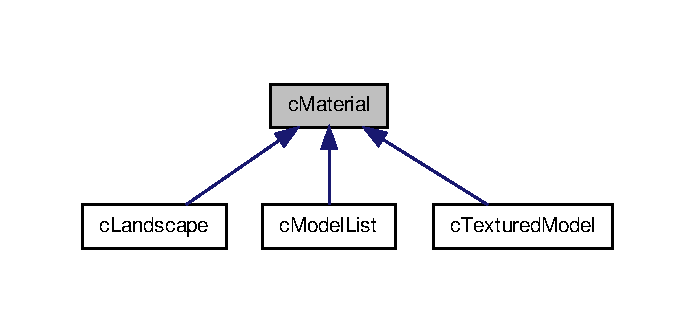
\includegraphics[width=334pt]{classc_material__inherit__graph}
\end{center}
\end{figure}
\subsection*{Public Member Functions}
\begin{DoxyCompactItemize}
\item 
\hyperlink{classc_material_acccfb25dd445a8279f0452dbe53f5079}{cMaterial} ()
\begin{DoxyCompactList}\small\item\em Will create a new material object. \item\end{DoxyCompactList}\item 
void \hyperlink{classc_material_aa08385e14417f023b8529ec491f5df38}{SetSpecular} (float lfRed, float lfGreen, float lfBlue, float lfAlpha)
\begin{DoxyCompactList}\small\item\em Will set the RGBA color of Specular reflections of this material (RGBA). \item\end{DoxyCompactList}\item 
void \hyperlink{classc_material_a7b3a800d84e017b955fd9faa9d7fda15}{SetShine} (float lfShine)
\begin{DoxyCompactList}\small\item\em Will set the shininess of this material (0.0f -\/ 1.0f). \item\end{DoxyCompactList}\item 
void \hyperlink{classc_material_af08e6f579a6c0e41490721320355a2f4}{PrepareMaterial} ()
\begin{DoxyCompactList}\small\item\em Will bind the material to OpenGL ready to be used. Once all the material variables are set, call this to prepare the material. \item\end{DoxyCompactList}\end{DoxyCompactItemize}


\subsection{Detailed Description}
A class to store material data for an object. Defines the 'reflectiveness' of the surface. 

Definition at line 5 of file WTcMaterial.h.



\subsection{Constructor \& Destructor Documentation}
\hypertarget{classc_material_acccfb25dd445a8279f0452dbe53f5079}{
\index{cMaterial@{cMaterial}!cMaterial@{cMaterial}}
\index{cMaterial@{cMaterial}!cMaterial@{cMaterial}}
\subsubsection[{cMaterial}]{\setlength{\rightskip}{0pt plus 5cm}cMaterial::cMaterial (
\begin{DoxyParamCaption}
{}
\end{DoxyParamCaption}
)}}
\label{classc_material_acccfb25dd445a8279f0452dbe53f5079}


Will create a new material object. 



Definition at line 4 of file WTcMaterial.cpp.



\subsection{Member Function Documentation}
\hypertarget{classc_material_af08e6f579a6c0e41490721320355a2f4}{
\index{cMaterial@{cMaterial}!PrepareMaterial@{PrepareMaterial}}
\index{PrepareMaterial@{PrepareMaterial}!cMaterial@{cMaterial}}
\subsubsection[{PrepareMaterial}]{\setlength{\rightskip}{0pt plus 5cm}void cMaterial::PrepareMaterial (
\begin{DoxyParamCaption}
{}
\end{DoxyParamCaption}
)}}
\label{classc_material_af08e6f579a6c0e41490721320355a2f4}


Will bind the material to OpenGL ready to be used. Once all the material variables are set, call this to prepare the material. 



Definition at line 26 of file WTcMaterial.cpp.

\hypertarget{classc_material_a7b3a800d84e017b955fd9faa9d7fda15}{
\index{cMaterial@{cMaterial}!SetShine@{SetShine}}
\index{SetShine@{SetShine}!cMaterial@{cMaterial}}
\subsubsection[{SetShine}]{\setlength{\rightskip}{0pt plus 5cm}void cMaterial::SetShine (
\begin{DoxyParamCaption}
\item[{float}]{lfShine}
\end{DoxyParamCaption}
)}}
\label{classc_material_a7b3a800d84e017b955fd9faa9d7fda15}


Will set the shininess of this material (0.0f -\/ 1.0f). 



Definition at line 21 of file WTcMaterial.cpp.

\hypertarget{classc_material_aa08385e14417f023b8529ec491f5df38}{
\index{cMaterial@{cMaterial}!SetSpecular@{SetSpecular}}
\index{SetSpecular@{SetSpecular}!cMaterial@{cMaterial}}
\subsubsection[{SetSpecular}]{\setlength{\rightskip}{0pt plus 5cm}void cMaterial::SetSpecular (
\begin{DoxyParamCaption}
\item[{float}]{lfRed, }
\item[{float}]{lfGreen, }
\item[{float}]{lfBlue, }
\item[{float}]{lfAlpha}
\end{DoxyParamCaption}
)}}
\label{classc_material_aa08385e14417f023b8529ec491f5df38}


Will set the RGBA color of Specular reflections of this material (RGBA). 



Definition at line 13 of file WTcMaterial.cpp.


\hypertarget{classc_matrix}{
\section{cMatrix Class Reference}
\label{classc_matrix}\index{cMatrix@{cMatrix}}
}
\subsection*{Public Member Functions}
\begin{DoxyCompactItemize}
\item 
\hyperlink{classc_matrix_a18b73c2c747b236d7ef9989acff7707a}{cMatrix} (int liRow, int liColumn)
\item 
void \hyperlink{classc_matrix_acb12737adff602163dffa098bf058105}{operator=} (\hyperlink{classc_matrix}{cMatrix} \&lVal)
\item 
void \hyperlink{classc_matrix_ac06926bba31e746c6946134cff767af3}{operator=} (float \&lVal)
\item 
void \hyperlink{classc_matrix_a9485d541a419175e8ea51b560eb910f1}{operator=} (const float lVal)
\item 
\hyperlink{classc_matrix}{cMatrix} \hyperlink{classc_matrix_ab72b22c4bed1e7acd694c1ce41756b47}{operator+} (\hyperlink{classc_matrix}{cMatrix} \&lVal)
\item 
\hyperlink{classc_matrix}{cMatrix} \hyperlink{classc_matrix_ad3a5d24417f057a1a900b5e78805c667}{operator+} (float \&lVal)
\item 
\hyperlink{classc_matrix}{cMatrix} \hyperlink{classc_matrix_a6848e16c55348f21244f4cda475e6c2b}{operator+} (const float lVal)
\item 
\hyperlink{classc_matrix}{cMatrix} \hyperlink{classc_matrix_a3db7778797b0bfafbc9f78c09b4114ee}{operator-\/} (\hyperlink{classc_matrix}{cMatrix} \&lVal)
\item 
\hyperlink{classc_matrix}{cMatrix} \hyperlink{classc_matrix_aec09028dd9d5de25967591ec9c538923}{operator-\/} (float \&lVal)
\item 
\hyperlink{classc_matrix}{cMatrix} \hyperlink{classc_matrix_a262976420f90ece91efbeb5bc7c9fd3b}{operator-\/} (const float lVal)
\item 
\hyperlink{classc_matrix}{cMatrix} \hyperlink{classc_matrix_a89176c84a903f423a4e309cb5c595a88}{operator$\ast$} (\hyperlink{classc_matrix}{cMatrix} \&lVal)
\item 
\hyperlink{classc_matrix}{cMatrix} \hyperlink{classc_matrix_afbb19919bf9bc2e9ed3ec907fe372cf2}{operator$\ast$} (float \&lVal)
\item 
\hyperlink{classc_matrix}{cMatrix} \hyperlink{classc_matrix_ac33872553efa9046c94951545ca4c733}{operator$\ast$} (const float lVal)
\item 
\hyperlink{classc_matrix}{cMatrix} \hyperlink{classc_matrix_a24369dee54a54e6df98f966f7af270d9}{operator/} (\hyperlink{classc_matrix}{cMatrix} \&lVal)
\item 
\hyperlink{classc_matrix}{cMatrix} \hyperlink{classc_matrix_a8f7b51e2bb65872a46544b6de36c31f9}{operator/} (float \&lVal)
\item 
\hyperlink{classc_matrix}{cMatrix} \hyperlink{classc_matrix_abcf6ed68df6879de7cba83ec82895b78}{operator/} (const float lVal)
\item 
bool \hyperlink{classc_matrix_aec3f3ce1f32891f528d488ec3b257b6b}{Equivalent} (\hyperlink{classc_matrix}{cMatrix} \&lVal)
\item 
\hyperlink{classc_matrix}{cMatrix} \hyperlink{classc_matrix_ac255cfade2876998d51702c1a50164dd}{Determinant} ()
\item 
\hyperlink{classc_matrix}{cMatrix} \hyperlink{classc_matrix_adc30d2a16fb44e2357d2163558f13358}{Transpose} ()
\end{DoxyCompactItemize}


\subsection{Detailed Description}


Definition at line 4 of file WTMatrixTemplate.h.



\subsection{Constructor \& Destructor Documentation}
\hypertarget{classc_matrix_a18b73c2c747b236d7ef9989acff7707a}{
\index{cMatrix@{cMatrix}!cMatrix@{cMatrix}}
\index{cMatrix@{cMatrix}!cMatrix@{cMatrix}}
\subsubsection[{cMatrix}]{\setlength{\rightskip}{0pt plus 5cm}cMatrix::cMatrix (
\begin{DoxyParamCaption}
\item[{int}]{liRow, }
\item[{int}]{liColumn}
\end{DoxyParamCaption}
)}}
\label{classc_matrix_a18b73c2c747b236d7ef9989acff7707a}


Definition at line 277 of file WTMatrixTemplate.h.



\subsection{Member Function Documentation}
\hypertarget{classc_matrix_ac255cfade2876998d51702c1a50164dd}{
\index{cMatrix@{cMatrix}!Determinant@{Determinant}}
\index{Determinant@{Determinant}!cMatrix@{cMatrix}}
\subsubsection[{Determinant}]{\setlength{\rightskip}{0pt plus 5cm}{\bf cMatrix} cMatrix::Determinant (
\begin{DoxyParamCaption}
{}
\end{DoxyParamCaption}
)}}
\label{classc_matrix_ac255cfade2876998d51702c1a50164dd}


Definition at line 54 of file WTMatrixTemplate.h.

\hypertarget{classc_matrix_aec3f3ce1f32891f528d488ec3b257b6b}{
\index{cMatrix@{cMatrix}!Equivalent@{Equivalent}}
\index{Equivalent@{Equivalent}!cMatrix@{cMatrix}}
\subsubsection[{Equivalent}]{\setlength{\rightskip}{0pt plus 5cm}bool cMatrix::Equivalent (
\begin{DoxyParamCaption}
\item[{{\bf cMatrix} \&}]{lVal}
\end{DoxyParamCaption}
)\hspace{0.3cm}{\ttfamily  \mbox{[}inline\mbox{]}}}}
\label{classc_matrix_aec3f3ce1f32891f528d488ec3b257b6b}


Definition at line 32 of file WTMatrixTemplate.h.

\hypertarget{classc_matrix_a89176c84a903f423a4e309cb5c595a88}{
\index{cMatrix@{cMatrix}!operator$\ast$@{operator$\ast$}}
\index{operator$\ast$@{operator$\ast$}!cMatrix@{cMatrix}}
\subsubsection[{operator$\ast$}]{\setlength{\rightskip}{0pt plus 5cm}{\bf cMatrix} cMatrix::operator$\ast$ (
\begin{DoxyParamCaption}
\item[{{\bf cMatrix} \&}]{lVal}
\end{DoxyParamCaption}
)}}
\label{classc_matrix_a89176c84a903f423a4e309cb5c595a88}
\hypertarget{classc_matrix_afbb19919bf9bc2e9ed3ec907fe372cf2}{
\index{cMatrix@{cMatrix}!operator$\ast$@{operator$\ast$}}
\index{operator$\ast$@{operator$\ast$}!cMatrix@{cMatrix}}
\subsubsection[{operator$\ast$}]{\setlength{\rightskip}{0pt plus 5cm}{\bf cMatrix} cMatrix::operator$\ast$ (
\begin{DoxyParamCaption}
\item[{float \&}]{lVal}
\end{DoxyParamCaption}
)}}
\label{classc_matrix_afbb19919bf9bc2e9ed3ec907fe372cf2}
\hypertarget{classc_matrix_ac33872553efa9046c94951545ca4c733}{
\index{cMatrix@{cMatrix}!operator$\ast$@{operator$\ast$}}
\index{operator$\ast$@{operator$\ast$}!cMatrix@{cMatrix}}
\subsubsection[{operator$\ast$}]{\setlength{\rightskip}{0pt plus 5cm}{\bf cMatrix} cMatrix::operator$\ast$ (
\begin{DoxyParamCaption}
\item[{const float}]{lVal}
\end{DoxyParamCaption}
)}}
\label{classc_matrix_ac33872553efa9046c94951545ca4c733}
\hypertarget{classc_matrix_ab72b22c4bed1e7acd694c1ce41756b47}{
\index{cMatrix@{cMatrix}!operator+@{operator+}}
\index{operator+@{operator+}!cMatrix@{cMatrix}}
\subsubsection[{operator+}]{\setlength{\rightskip}{0pt plus 5cm}{\bf cMatrix} cMatrix::operator+ (
\begin{DoxyParamCaption}
\item[{{\bf cMatrix} \&}]{lVal}
\end{DoxyParamCaption}
)}}
\label{classc_matrix_ab72b22c4bed1e7acd694c1ce41756b47}


Definition at line 88 of file WTMatrixTemplate.h.

\hypertarget{classc_matrix_ad3a5d24417f057a1a900b5e78805c667}{
\index{cMatrix@{cMatrix}!operator+@{operator+}}
\index{operator+@{operator+}!cMatrix@{cMatrix}}
\subsubsection[{operator+}]{\setlength{\rightskip}{0pt plus 5cm}{\bf cMatrix} cMatrix::operator+ (
\begin{DoxyParamCaption}
\item[{float \&}]{lVal}
\end{DoxyParamCaption}
)}}
\label{classc_matrix_ad3a5d24417f057a1a900b5e78805c667}


Definition at line 103 of file WTMatrixTemplate.h.

\hypertarget{classc_matrix_a6848e16c55348f21244f4cda475e6c2b}{
\index{cMatrix@{cMatrix}!operator+@{operator+}}
\index{operator+@{operator+}!cMatrix@{cMatrix}}
\subsubsection[{operator+}]{\setlength{\rightskip}{0pt plus 5cm}{\bf cMatrix} cMatrix::operator+ (
\begin{DoxyParamCaption}
\item[{const float}]{lVal}
\end{DoxyParamCaption}
)}}
\label{classc_matrix_a6848e16c55348f21244f4cda475e6c2b}


Definition at line 114 of file WTMatrixTemplate.h.

\hypertarget{classc_matrix_aec09028dd9d5de25967591ec9c538923}{
\index{cMatrix@{cMatrix}!operator-\/@{operator-\/}}
\index{operator-\/@{operator-\/}!cMatrix@{cMatrix}}
\subsubsection[{operator-\/}]{\setlength{\rightskip}{0pt plus 5cm}{\bf cMatrix} cMatrix::operator-\/ (
\begin{DoxyParamCaption}
\item[{float \&}]{lVal}
\end{DoxyParamCaption}
)}}
\label{classc_matrix_aec09028dd9d5de25967591ec9c538923}


Definition at line 140 of file WTMatrixTemplate.h.

\hypertarget{classc_matrix_a262976420f90ece91efbeb5bc7c9fd3b}{
\index{cMatrix@{cMatrix}!operator-\/@{operator-\/}}
\index{operator-\/@{operator-\/}!cMatrix@{cMatrix}}
\subsubsection[{operator-\/}]{\setlength{\rightskip}{0pt plus 5cm}{\bf cMatrix} cMatrix::operator-\/ (
\begin{DoxyParamCaption}
\item[{const float}]{lVal}
\end{DoxyParamCaption}
)}}
\label{classc_matrix_a262976420f90ece91efbeb5bc7c9fd3b}


Definition at line 151 of file WTMatrixTemplate.h.

\hypertarget{classc_matrix_a3db7778797b0bfafbc9f78c09b4114ee}{
\index{cMatrix@{cMatrix}!operator-\/@{operator-\/}}
\index{operator-\/@{operator-\/}!cMatrix@{cMatrix}}
\subsubsection[{operator-\/}]{\setlength{\rightskip}{0pt plus 5cm}{\bf cMatrix} cMatrix::operator-\/ (
\begin{DoxyParamCaption}
\item[{{\bf cMatrix} \&}]{lVal}
\end{DoxyParamCaption}
)}}
\label{classc_matrix_a3db7778797b0bfafbc9f78c09b4114ee}


Definition at line 125 of file WTMatrixTemplate.h.

\hypertarget{classc_matrix_a24369dee54a54e6df98f966f7af270d9}{
\index{cMatrix@{cMatrix}!operator/@{operator/}}
\index{operator/@{operator/}!cMatrix@{cMatrix}}
\subsubsection[{operator/}]{\setlength{\rightskip}{0pt plus 5cm}{\bf cMatrix} cMatrix::operator/ (
\begin{DoxyParamCaption}
\item[{{\bf cMatrix} \&}]{lVal}
\end{DoxyParamCaption}
)}}
\label{classc_matrix_a24369dee54a54e6df98f966f7af270d9}
\hypertarget{classc_matrix_a8f7b51e2bb65872a46544b6de36c31f9}{
\index{cMatrix@{cMatrix}!operator/@{operator/}}
\index{operator/@{operator/}!cMatrix@{cMatrix}}
\subsubsection[{operator/}]{\setlength{\rightskip}{0pt plus 5cm}{\bf cMatrix} cMatrix::operator/ (
\begin{DoxyParamCaption}
\item[{float \&}]{lVal}
\end{DoxyParamCaption}
)}}
\label{classc_matrix_a8f7b51e2bb65872a46544b6de36c31f9}
\hypertarget{classc_matrix_abcf6ed68df6879de7cba83ec82895b78}{
\index{cMatrix@{cMatrix}!operator/@{operator/}}
\index{operator/@{operator/}!cMatrix@{cMatrix}}
\subsubsection[{operator/}]{\setlength{\rightskip}{0pt plus 5cm}{\bf cMatrix} cMatrix::operator/ (
\begin{DoxyParamCaption}
\item[{const float}]{lVal}
\end{DoxyParamCaption}
)}}
\label{classc_matrix_abcf6ed68df6879de7cba83ec82895b78}
\hypertarget{classc_matrix_ac06926bba31e746c6946134cff767af3}{
\index{cMatrix@{cMatrix}!operator=@{operator=}}
\index{operator=@{operator=}!cMatrix@{cMatrix}}
\subsubsection[{operator=}]{\setlength{\rightskip}{0pt plus 5cm}void cMatrix::operator= (
\begin{DoxyParamCaption}
\item[{float \&}]{lVal}
\end{DoxyParamCaption}
)}}
\label{classc_matrix_ac06926bba31e746c6946134cff767af3}


Definition at line 70 of file WTMatrixTemplate.h.

\hypertarget{classc_matrix_acb12737adff602163dffa098bf058105}{
\index{cMatrix@{cMatrix}!operator=@{operator=}}
\index{operator=@{operator=}!cMatrix@{cMatrix}}
\subsubsection[{operator=}]{\setlength{\rightskip}{0pt plus 5cm}void cMatrix::operator= (
\begin{DoxyParamCaption}
\item[{{\bf cMatrix} \&}]{lVal}
\end{DoxyParamCaption}
)}}
\label{classc_matrix_acb12737adff602163dffa098bf058105}


Definition at line 59 of file WTMatrixTemplate.h.

\hypertarget{classc_matrix_a9485d541a419175e8ea51b560eb910f1}{
\index{cMatrix@{cMatrix}!operator=@{operator=}}
\index{operator=@{operator=}!cMatrix@{cMatrix}}
\subsubsection[{operator=}]{\setlength{\rightskip}{0pt plus 5cm}void cMatrix::operator= (
\begin{DoxyParamCaption}
\item[{const float}]{lVal}
\end{DoxyParamCaption}
)}}
\label{classc_matrix_a9485d541a419175e8ea51b560eb910f1}


Definition at line 79 of file WTMatrixTemplate.h.

\hypertarget{classc_matrix_adc30d2a16fb44e2357d2163558f13358}{
\index{cMatrix@{cMatrix}!Transpose@{Transpose}}
\index{Transpose@{Transpose}!cMatrix@{cMatrix}}
\subsubsection[{Transpose}]{\setlength{\rightskip}{0pt plus 5cm}{\bf cMatrix} cMatrix::Transpose (
\begin{DoxyParamCaption}
{}
\end{DoxyParamCaption}
)}}
\label{classc_matrix_adc30d2a16fb44e2357d2163558f13358}


Definition at line 39 of file WTMatrixTemplate.h.


\hypertarget{classc_matrix4}{
\section{cMatrix4 Class Reference}
\label{classc_matrix4}\index{cMatrix4@{cMatrix4}}
}


this is a standard 4x4 translation matrix for objects. This is a standard 4x4 translation matrix for objects. It can be used for both 2D and 3D objects. By default it is a 3D matrix, It can be converted to a 2D matrix by using the function \hyperlink{classc_matrix4_ad24236403317622459c3309938be9d21}{Set2D()}. The matrix Layout is four columns, each one representing a different axis or translation. Xx, Xy, Xz, 0.0f, Yx Yy Yz 0.0f, Zx Zy Zx 0.0f, Px, Py, Pz, 1.0f  




Collaboration diagram for cMatrix4:\nopagebreak
\begin{figure}[H]
\begin{center}
\leavevmode
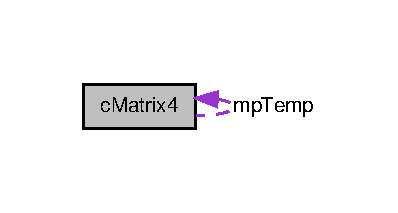
\includegraphics[width=191pt]{classc_matrix4__coll__graph}
\end{center}
\end{figure}
\subsection*{Public Member Functions}
\begin{DoxyCompactItemize}
\item 
\hypertarget{classc_matrix4_af728db2d340a48de20d9f9e143e3a19b}{
void \hyperlink{classc_matrix4_af728db2d340a48de20d9f9e143e3a19b}{Translate} (float lfX, float lfY, float lfZ)}
\label{classc_matrix4_af728db2d340a48de20d9f9e143e3a19b}

\begin{DoxyCompactList}\small\item\em This will move the Object along the local axis the distance of lfX, lfY and lfZ. \end{DoxyCompactList}\item 
\hypertarget{classc_matrix4_a70935a369368c343c32efe6c47877e03}{
void \hyperlink{classc_matrix4_a70935a369368c343c32efe6c47877e03}{Translate} (float $\ast$lpDist)}
\label{classc_matrix4_a70935a369368c343c32efe6c47877e03}

\begin{DoxyCompactList}\small\item\em This will move the Object along the local axis the distance of the array of three floats pointed to by lpDist. \end{DoxyCompactList}\item 
\hypertarget{classc_matrix4_a8697973a28e45b0866cce4cdba2e216d}{
float $\ast$ \hyperlink{classc_matrix4_a8697973a28e45b0866cce4cdba2e216d}{Matrix} ()}
\label{classc_matrix4_a8697973a28e45b0866cce4cdba2e216d}

\begin{DoxyCompactList}\small\item\em This will return a pointer to this objects matrix data. \end{DoxyCompactList}\item 
\hypertarget{classc_matrix4_a1e70788aed256a22cf62b11a12e0db74}{
float $\ast$ \hyperlink{classc_matrix4_a1e70788aed256a22cf62b11a12e0db74}{Matrix} (uint8 lcData)}
\label{classc_matrix4_a1e70788aed256a22cf62b11a12e0db74}

\begin{DoxyCompactList}\small\item\em This will return a pointer to the float numbered lcData in this objects matrix. \end{DoxyCompactList}\item 
\hypertarget{classc_matrix4_a7b0917b0f0a69d73ed41d05fd37d52ac}{
float $\ast$ \hyperlink{classc_matrix4_a7b0917b0f0a69d73ed41d05fd37d52ac}{Position} ()}
\label{classc_matrix4_a7b0917b0f0a69d73ed41d05fd37d52ac}

\begin{DoxyCompactList}\small\item\em This will reutrn a pointer to this objects matrices position vector. \end{DoxyCompactList}\item 
\hypertarget{classc_matrix4_aff5d7d1cf3cf0b9ddb9e55e2f799012f}{
float \hyperlink{classc_matrix4_aff5d7d1cf3cf0b9ddb9e55e2f799012f}{X} ()}
\label{classc_matrix4_aff5d7d1cf3cf0b9ddb9e55e2f799012f}

\begin{DoxyCompactList}\small\item\em This will return this objects X position value. \end{DoxyCompactList}\item 
\hypertarget{classc_matrix4_aa22f36646d19566a438a297cb9a9bfb5}{
float \hyperlink{classc_matrix4_aa22f36646d19566a438a297cb9a9bfb5}{Y} ()}
\label{classc_matrix4_aa22f36646d19566a438a297cb9a9bfb5}

\begin{DoxyCompactList}\small\item\em This will return this objects Y position value. \end{DoxyCompactList}\item 
\hypertarget{classc_matrix4_a8b62f500f8194b06dab12e85e57fd9ef}{
float \hyperlink{classc_matrix4_a8b62f500f8194b06dab12e85e57fd9ef}{Z} ()}
\label{classc_matrix4_a8b62f500f8194b06dab12e85e57fd9ef}

\begin{DoxyCompactList}\small\item\em This will return this objects Z position value. \end{DoxyCompactList}\item 
\hypertarget{classc_matrix4_a958689f28a118eac91104f5a847ac0fd}{
float $\ast$ \hyperlink{classc_matrix4_a958689f28a118eac91104f5a847ac0fd}{XVect} ()}
\label{classc_matrix4_a958689f28a118eac91104f5a847ac0fd}

\begin{DoxyCompactList}\small\item\em This will return the vector along this objects local X axis. \end{DoxyCompactList}\item 
\hypertarget{classc_matrix4_acff0242ac76b2ccd854eeec0d4913abe}{
float $\ast$ \hyperlink{classc_matrix4_acff0242ac76b2ccd854eeec0d4913abe}{YVect} ()}
\label{classc_matrix4_acff0242ac76b2ccd854eeec0d4913abe}

\begin{DoxyCompactList}\small\item\em This will return the vector along this objects local Y axis. \end{DoxyCompactList}\item 
\hypertarget{classc_matrix4_ab3d5e1a9ca6652c84265d4d164494699}{
float $\ast$ \hyperlink{classc_matrix4_ab3d5e1a9ca6652c84265d4d164494699}{ZVect} ()}
\label{classc_matrix4_ab3d5e1a9ca6652c84265d4d164494699}

\begin{DoxyCompactList}\small\item\em This will return the vector along this objects local Z axis. \end{DoxyCompactList}\item 
\hypertarget{classc_matrix4_a46a1fd03c71ffc4554f2a0f611260d84}{
float \hyperlink{classc_matrix4_a46a1fd03c71ffc4554f2a0f611260d84}{Xx} ()}
\label{classc_matrix4_a46a1fd03c71ffc4554f2a0f611260d84}

\begin{DoxyCompactList}\small\item\em X Component of the X axis. \end{DoxyCompactList}\item 
\hypertarget{classc_matrix4_ab345450c98494d70efcc2cdc0bdd90f6}{
float \hyperlink{classc_matrix4_ab345450c98494d70efcc2cdc0bdd90f6}{Xy} ()}
\label{classc_matrix4_ab345450c98494d70efcc2cdc0bdd90f6}

\begin{DoxyCompactList}\small\item\em Y Component of the X axis. \end{DoxyCompactList}\item 
\hypertarget{classc_matrix4_a9acdcdf379f77a0ec47214620e1a5f9a}{
float \hyperlink{classc_matrix4_a9acdcdf379f77a0ec47214620e1a5f9a}{Xz} ()}
\label{classc_matrix4_a9acdcdf379f77a0ec47214620e1a5f9a}

\begin{DoxyCompactList}\small\item\em Z Component of the X axis. \end{DoxyCompactList}\item 
\hypertarget{classc_matrix4_af4dc361f269ecd60238ce0b647313504}{
float \hyperlink{classc_matrix4_af4dc361f269ecd60238ce0b647313504}{Yx} ()}
\label{classc_matrix4_af4dc361f269ecd60238ce0b647313504}

\begin{DoxyCompactList}\small\item\em X Component of the Y axis. \end{DoxyCompactList}\item 
\hypertarget{classc_matrix4_a4f8182f7b1ec729250c500b1ac9c0696}{
float \hyperlink{classc_matrix4_a4f8182f7b1ec729250c500b1ac9c0696}{Yy} ()}
\label{classc_matrix4_a4f8182f7b1ec729250c500b1ac9c0696}

\begin{DoxyCompactList}\small\item\em Y Component of the Y axis. \end{DoxyCompactList}\item 
\hypertarget{classc_matrix4_ad81766f34027dcc5d22d45b927275280}{
float \hyperlink{classc_matrix4_ad81766f34027dcc5d22d45b927275280}{Yz} ()}
\label{classc_matrix4_ad81766f34027dcc5d22d45b927275280}

\begin{DoxyCompactList}\small\item\em Z Component of the Y axis. \end{DoxyCompactList}\item 
\hypertarget{classc_matrix4_a12829c26cfd157917540d7389345a56a}{
float \hyperlink{classc_matrix4_a12829c26cfd157917540d7389345a56a}{Zx} ()}
\label{classc_matrix4_a12829c26cfd157917540d7389345a56a}

\begin{DoxyCompactList}\small\item\em X Component of the Z axis. \end{DoxyCompactList}\item 
\hypertarget{classc_matrix4_a0c2541f2d0050322f2c28e1c5efce327}{
float \hyperlink{classc_matrix4_a0c2541f2d0050322f2c28e1c5efce327}{Zy} ()}
\label{classc_matrix4_a0c2541f2d0050322f2c28e1c5efce327}

\begin{DoxyCompactList}\small\item\em Y Component of the Z axis. \end{DoxyCompactList}\item 
\hypertarget{classc_matrix4_a7d4ef2375b3a6bf5a3d9728aee1ba752}{
float \hyperlink{classc_matrix4_a7d4ef2375b3a6bf5a3d9728aee1ba752}{Zz} ()}
\label{classc_matrix4_a7d4ef2375b3a6bf5a3d9728aee1ba752}

\begin{DoxyCompactList}\small\item\em Z Component of the Z axis. \end{DoxyCompactList}\item 
\hypertarget{classc_matrix4_ae3bb670db30cee45d59aef1599289086}{
void \hyperlink{classc_matrix4_ae3bb670db30cee45d59aef1599289086}{Position} (float $\ast$lpPos)}
\label{classc_matrix4_ae3bb670db30cee45d59aef1599289086}

\begin{DoxyCompactList}\small\item\em This will take 2 or three floats depending if this \hyperlink{classc_matrix4}{cMatrix4} is set to 2D or 3D operations and set the position of the object. \end{DoxyCompactList}\item 
\hypertarget{classc_matrix4_adf27db7265e42ccbbb5a6779800c39ea}{
void \hyperlink{classc_matrix4_adf27db7265e42ccbbb5a6779800c39ea}{PositionX} (float lfX)}
\label{classc_matrix4_adf27db7265e42ccbbb5a6779800c39ea}

\begin{DoxyCompactList}\small\item\em This will set the objects X position to be equal to lfX. \end{DoxyCompactList}\item 
\hypertarget{classc_matrix4_a4f7469486d7557e158ebc70a261c853c}{
void \hyperlink{classc_matrix4_a4f7469486d7557e158ebc70a261c853c}{PositionY} (float lfY)}
\label{classc_matrix4_a4f7469486d7557e158ebc70a261c853c}

\begin{DoxyCompactList}\small\item\em This will set the objects Y position to be equal to lfX. \end{DoxyCompactList}\item 
\hypertarget{classc_matrix4_a6baf253feb5e27b5e3e81971d9f5d718}{
void \hyperlink{classc_matrix4_a6baf253feb5e27b5e3e81971d9f5d718}{PositionZ} (float lfZ)}
\label{classc_matrix4_a6baf253feb5e27b5e3e81971d9f5d718}

\begin{DoxyCompactList}\small\item\em This will set the objects Z position to be equal to lfX. \end{DoxyCompactList}\item 
\hypertarget{classc_matrix4_a79457e17d6ab9a0c5db16c94405be35c}{
void \hyperlink{classc_matrix4_a79457e17d6ab9a0c5db16c94405be35c}{Position} (\hyperlink{classc_matrix4}{cMatrix4} \&lpOther)}
\label{classc_matrix4_a79457e17d6ab9a0c5db16c94405be35c}

\begin{DoxyCompactList}\small\item\em This will make this object have the same Position as the \hyperlink{classc_matrix4}{cMatrix4} lpOther. \end{DoxyCompactList}\item 
\hypertarget{classc_matrix4_a6e0051199566d89193d7c2e07e957eb4}{
void \hyperlink{classc_matrix4_a6e0051199566d89193d7c2e07e957eb4}{Position} (\hyperlink{classc_matrix4}{cMatrix4} $\ast$lpOther)}
\label{classc_matrix4_a6e0051199566d89193d7c2e07e957eb4}

\begin{DoxyCompactList}\small\item\em Will copy the position data from the matrix lpOther. \end{DoxyCompactList}\item 
\hypertarget{classc_matrix4_ac182a447e047d9071b035b374e8abf45}{
void \hyperlink{classc_matrix4_ac182a447e047d9071b035b374e8abf45}{Position} (c2DVf $\ast$lpPosition)}
\label{classc_matrix4_ac182a447e047d9071b035b374e8abf45}

\begin{DoxyCompactList}\small\item\em This will position the current object to the 2D Vector lpPosition. (X,Y) \end{DoxyCompactList}\item 
\hypertarget{classc_matrix4_a81cd364d37dc5eae6f968551331ad7a3}{
void \hyperlink{classc_matrix4_a81cd364d37dc5eae6f968551331ad7a3}{Position} (float lfX, float lfY)}
\label{classc_matrix4_a81cd364d37dc5eae6f968551331ad7a3}

\begin{DoxyCompactList}\small\item\em This will position the current object to lfX,lfY. (X,Y) \end{DoxyCompactList}\item 
\hypertarget{classc_matrix4_a8a49976693c27e4fbb5fce427eb6bcf5}{
void \hyperlink{classc_matrix4_a8a49976693c27e4fbb5fce427eb6bcf5}{Position} (c3DVf $\ast$lpPosition)}
\label{classc_matrix4_a8a49976693c27e4fbb5fce427eb6bcf5}

\begin{DoxyCompactList}\small\item\em This will position the current object to the 3D Vector lpPosition. (X,Y,Z) \end{DoxyCompactList}\item 
\hypertarget{classc_matrix4_ae404d9b94cb676d9896385fef1eda422}{
void \hyperlink{classc_matrix4_ae404d9b94cb676d9896385fef1eda422}{Position} (float lfX, float lfY, float lfZ)}
\label{classc_matrix4_ae404d9b94cb676d9896385fef1eda422}

\begin{DoxyCompactList}\small\item\em This will position the current object to lfX,lfY,lfX. (X,Y,Z) \end{DoxyCompactList}\item 
\hypertarget{classc_matrix4_a91f9e8d79d7721ba35f59c754a5507d1}{
void \hyperlink{classc_matrix4_a91f9e8d79d7721ba35f59c754a5507d1}{Advance} (float $\ast$lfDistance)}
\label{classc_matrix4_a91f9e8d79d7721ba35f59c754a5507d1}

\begin{DoxyCompactList}\small\item\em Will Advance the object along its local axis by the distance of the floats in the array lfDistance. \end{DoxyCompactList}\item 
\hypertarget{classc_matrix4_a6c53b28448e2d2531a19cd49955f5901}{
void \hyperlink{classc_matrix4_a6c53b28448e2d2531a19cd49955f5901}{Advance} (c2DVf $\ast$lfDistances)}
\label{classc_matrix4_a6c53b28448e2d2531a19cd49955f5901}

\begin{DoxyCompactList}\small\item\em Will Advance the object along its local X and Y axis by the Vector lfDistances;. \end{DoxyCompactList}\item 
\hypertarget{classc_matrix4_a86aefa3a444eaabd4ad1a66e4857f40e}{
void \hyperlink{classc_matrix4_a86aefa3a444eaabd4ad1a66e4857f40e}{Advance} (c3DVf $\ast$lfDistances)}
\label{classc_matrix4_a86aefa3a444eaabd4ad1a66e4857f40e}

\begin{DoxyCompactList}\small\item\em Will Advance the object along its local X, Y and Z axis by the Vector lfDistances;. \end{DoxyCompactList}\item 
\hypertarget{classc_matrix4_a07d410e6592dacf244ad118d70443181}{
void \hyperlink{classc_matrix4_a07d410e6592dacf244ad118d70443181}{Advance} (c2DVf \&lfDistances)}
\label{classc_matrix4_a07d410e6592dacf244ad118d70443181}

\begin{DoxyCompactList}\small\item\em Will Advance the object along its local X and Y axis by the Vector lfDistances;. \end{DoxyCompactList}\item 
\hypertarget{classc_matrix4_ac07dd71793d6df522efa2098f9e1daa6}{
void \hyperlink{classc_matrix4_ac07dd71793d6df522efa2098f9e1daa6}{Advance} (c3DVf \&lfDistances)}
\label{classc_matrix4_ac07dd71793d6df522efa2098f9e1daa6}

\begin{DoxyCompactList}\small\item\em Will Advance the object along its local X, Y and Z axis by the Vector lfDistances;. \end{DoxyCompactList}\item 
\hypertarget{classc_matrix4_ad0744229e75d1053c3a2e4bcfe8dc46f}{
void \hyperlink{classc_matrix4_ad0744229e75d1053c3a2e4bcfe8dc46f}{Advance} (float lfDistance)}
\label{classc_matrix4_ad0744229e75d1053c3a2e4bcfe8dc46f}

\begin{DoxyCompactList}\small\item\em This will advance an object along the (2D or 3D) Vector that is its facing by a distance of lfDistance;. \end{DoxyCompactList}\item 
\hypertarget{classc_matrix4_aa23f7d55e4eddcba673f8a6e44f63c3e}{
void \hyperlink{classc_matrix4_aa23f7d55e4eddcba673f8a6e44f63c3e}{AdvanceX} (float lfDistance)}
\label{classc_matrix4_aa23f7d55e4eddcba673f8a6e44f63c3e}

\begin{DoxyCompactList}\small\item\em This will advance the object along its local X axis by lfDistance. \end{DoxyCompactList}\item 
\hypertarget{classc_matrix4_ae28d0f2cfe996ec5422cdaec98f30c9a}{
void \hyperlink{classc_matrix4_ae28d0f2cfe996ec5422cdaec98f30c9a}{AdvanceY} (float lfDistance)}
\label{classc_matrix4_ae28d0f2cfe996ec5422cdaec98f30c9a}

\begin{DoxyCompactList}\small\item\em This will advance the object along its local Y axis by lfDistance. \end{DoxyCompactList}\item 
\hypertarget{classc_matrix4_a31d0d26e3b91628365871ad10dc33f8e}{
void \hyperlink{classc_matrix4_a31d0d26e3b91628365871ad10dc33f8e}{AdvanceZ} (float lfDistance)}
\label{classc_matrix4_a31d0d26e3b91628365871ad10dc33f8e}

\begin{DoxyCompactList}\small\item\em This will advance the object along its local Z axis by lfDistance. \end{DoxyCompactList}\item 
\hypertarget{classc_matrix4_ab956ec27a465b889126632475fd7d703}{
void \hyperlink{classc_matrix4_ab956ec27a465b889126632475fd7d703}{Advance} (float lfX, float lfY)}
\label{classc_matrix4_ab956ec27a465b889126632475fd7d703}

\begin{DoxyCompactList}\small\item\em This will move this matrix along its local X and Y axis by lfX and lfY respectively. Suitable for 2D objects. \end{DoxyCompactList}\item 
\hypertarget{classc_matrix4_a00d27c2daab0e05c403c8fb86445fb81}{
void \hyperlink{classc_matrix4_a00d27c2daab0e05c403c8fb86445fb81}{Advance} (float lfX, float lfY, float lfZ)}
\label{classc_matrix4_a00d27c2daab0e05c403c8fb86445fb81}

\begin{DoxyCompactList}\small\item\em This will advance the object along its local X, Y and Z axis by lfX, lfY and lfZ. \end{DoxyCompactList}\item 
\hypertarget{classc_matrix4_a92335a0e15b30c55f4838f1ab3dea1af}{
void \hyperlink{classc_matrix4_a92335a0e15b30c55f4838f1ab3dea1af}{GAdvance} (float $\ast$lfDistance)}
\label{classc_matrix4_a92335a0e15b30c55f4838f1ab3dea1af}

\begin{DoxyCompactList}\small\item\em Will Advance the object along its global axis by the distance of the floats in the array lfDistance. \end{DoxyCompactList}\item 
\hypertarget{classc_matrix4_a6796b615c465903d48fe0c8094b1f7c1}{
void \hyperlink{classc_matrix4_a6796b615c465903d48fe0c8094b1f7c1}{GAdvanceX} (float lfX)}
\label{classc_matrix4_a6796b615c465903d48fe0c8094b1f7c1}

\begin{DoxyCompactList}\small\item\em This will advance the object along the global X axis by lfX. \end{DoxyCompactList}\item 
\hypertarget{classc_matrix4_af4453f95ef875b0c5002d72bade65bb1}{
void \hyperlink{classc_matrix4_af4453f95ef875b0c5002d72bade65bb1}{GAdvanceY} (float lfX)}
\label{classc_matrix4_af4453f95ef875b0c5002d72bade65bb1}

\begin{DoxyCompactList}\small\item\em This will advance the object along the global Y axis by lfX. \end{DoxyCompactList}\item 
\hypertarget{classc_matrix4_a0fd4e894762e73050e8e2e38acdfaf0d}{
void \hyperlink{classc_matrix4_a0fd4e894762e73050e8e2e38acdfaf0d}{GAdvanceZ} (float lfX)}
\label{classc_matrix4_a0fd4e894762e73050e8e2e38acdfaf0d}

\begin{DoxyCompactList}\small\item\em This will advance the object along the global Z axis by lfX. \end{DoxyCompactList}\item 
\hypertarget{classc_matrix4_a2dc12cbe708c7bc63ca2beff47c0c835}{
void \hyperlink{classc_matrix4_a2dc12cbe708c7bc63ca2beff47c0c835}{GAdvance} (float lfX, float lfY)}
\label{classc_matrix4_a2dc12cbe708c7bc63ca2beff47c0c835}

\begin{DoxyCompactList}\small\item\em This will move this matrix along its global X and Y axis by lfX and lfY respectively. \end{DoxyCompactList}\item 
\hypertarget{classc_matrix4_ac1c16ceb7ac4c2f771fc0d4662df643c}{
void \hyperlink{classc_matrix4_ac1c16ceb7ac4c2f771fc0d4662df643c}{GAdvance} (float lfX, float lfY, float lfZ)}
\label{classc_matrix4_ac1c16ceb7ac4c2f771fc0d4662df643c}

\begin{DoxyCompactList}\small\item\em This will advance the object along the global X, Y and Z axis by lfX, lfY and lfZ. \end{DoxyCompactList}\item 
\hypertarget{classc_matrix4_ac86eb165802e359a11ace5db20b73c72}{
void \hyperlink{classc_matrix4_ac86eb165802e359a11ace5db20b73c72}{Angle} (float lfAngle)}
\label{classc_matrix4_ac86eb165802e359a11ace5db20b73c72}

\begin{DoxyCompactList}\small\item\em This will set the angle of rotation about this matrices X axis to lfAngle radians. Suitable for 2D objects. \end{DoxyCompactList}\item 
\hypertarget{classc_matrix4_a04a196147274eb6b3d1aca1782c26091}{
void \hyperlink{classc_matrix4_a04a196147274eb6b3d1aca1782c26091}{GRotateOrigin} (float lfAngle)}
\label{classc_matrix4_a04a196147274eb6b3d1aca1782c26091}

\begin{DoxyCompactList}\small\item\em This will rotate this matrix in the X axis through 0,0 by lfAngle radians. Suitable for 2D objects. \end{DoxyCompactList}\item 
\hypertarget{classc_matrix4_a5115db44a0c51d97be3d5791fb19d18a}{
void \hyperlink{classc_matrix4_a5115db44a0c51d97be3d5791fb19d18a}{GRotate} (float lfAngle, float lfX, float lfY)}
\label{classc_matrix4_a5115db44a0c51d97be3d5791fb19d18a}

\begin{DoxyCompactList}\small\item\em This will rotate this matrix in the X axis through lfX,lfY by lfAngle radians. Suitable for 2D objects. \end{DoxyCompactList}\item 
\hypertarget{classc_matrix4_aeca3db3711d09781ec4ecf78a0423574}{
void \hyperlink{classc_matrix4_aeca3db3711d09781ec4ecf78a0423574}{Rotation} (float $\ast$lpRotation)}
\label{classc_matrix4_aeca3db3711d09781ec4ecf78a0423574}

\begin{DoxyCompactList}\small\item\em Will copy the rotation of the matrix lpRotation. \end{DoxyCompactList}\item 
\hypertarget{classc_matrix4_a2777b2361f3656d4f8c1413456ea22d2}{
void \hyperlink{classc_matrix4_a2777b2361f3656d4f8c1413456ea22d2}{Rotation} (\hyperlink{classc_matrix4}{cMatrix4} $\ast$lpRotation)}
\label{classc_matrix4_a2777b2361f3656d4f8c1413456ea22d2}

\begin{DoxyCompactList}\small\item\em Will copy the rotation of the matrix lpRotation. \end{DoxyCompactList}\item 
\hypertarget{classc_matrix4_aa3eadfc363f0d3696e8f9468ccd3782b}{
void \hyperlink{classc_matrix4_aa3eadfc363f0d3696e8f9468ccd3782b}{Rotation} (\hyperlink{classc_matrix4}{cMatrix4} \&lpOther)}
\label{classc_matrix4_aa3eadfc363f0d3696e8f9468ccd3782b}

\begin{DoxyCompactList}\small\item\em This will make this object have the same Rotation as the \hyperlink{classc_matrix4}{cMatrix4} lpOther. \end{DoxyCompactList}\item 
\hypertarget{classc_matrix4_ab21d0553250b8ca4b0388105afc79478}{
void \hyperlink{classc_matrix4_ab21d0553250b8ca4b0388105afc79478}{Rotate} (float lfAngle)}
\label{classc_matrix4_ab21d0553250b8ca4b0388105afc79478}

\begin{DoxyCompactList}\small\item\em This will rotate the object around its local Z axis by lfAngle radians. Suitable for 2D objects. \end{DoxyCompactList}\item 
\hypertarget{classc_matrix4_af3c238c3d65276912b3071c33c9a8e59}{
void \hyperlink{classc_matrix4_af3c238c3d65276912b3071c33c9a8e59}{RotateX} (float lfAngle)}
\label{classc_matrix4_af3c238c3d65276912b3071c33c9a8e59}

\begin{DoxyCompactList}\small\item\em This will rotate the object around its local X axis by lfAngle radians. \end{DoxyCompactList}\item 
\hypertarget{classc_matrix4_ac625c531c3644462cc91ed53bef5e1e9}{
void \hyperlink{classc_matrix4_ac625c531c3644462cc91ed53bef5e1e9}{RotateY} (float lfAngle)}
\label{classc_matrix4_ac625c531c3644462cc91ed53bef5e1e9}

\begin{DoxyCompactList}\small\item\em This will rotate the object around its local Y axis by lfAngle radians. \end{DoxyCompactList}\item 
\hypertarget{classc_matrix4_a784f4dd7106e393b654d17ff78cc49a7}{
void \hyperlink{classc_matrix4_a784f4dd7106e393b654d17ff78cc49a7}{RotateZ} (float lfAngle)}
\label{classc_matrix4_a784f4dd7106e393b654d17ff78cc49a7}

\begin{DoxyCompactList}\small\item\em This will rotate the object around its local Z axis by lfAngle radians. \end{DoxyCompactList}\item 
\hypertarget{classc_matrix4_a0be08400d130f819bbedbb35f551d4c7}{
void \hyperlink{classc_matrix4_a0be08400d130f819bbedbb35f551d4c7}{GRotateX} (float lfAngle)}
\label{classc_matrix4_a0be08400d130f819bbedbb35f551d4c7}

\begin{DoxyCompactList}\small\item\em This will rotate the object around its global X axis by lfAngle radians. \end{DoxyCompactList}\item 
\hypertarget{classc_matrix4_a0ae1a3c85f3b00127217b67c7d75a7cc}{
void \hyperlink{classc_matrix4_a0ae1a3c85f3b00127217b67c7d75a7cc}{GRotateY} (float lfAngle)}
\label{classc_matrix4_a0ae1a3c85f3b00127217b67c7d75a7cc}

\begin{DoxyCompactList}\small\item\em This will rotate the object around its global X axis by lfAngle radians. \end{DoxyCompactList}\item 
\hypertarget{classc_matrix4_a1d082ca0f1c634d262309eb75a9e2df5}{
void \hyperlink{classc_matrix4_a1d082ca0f1c634d262309eb75a9e2df5}{GRotateZ} (float lfAngle)}
\label{classc_matrix4_a1d082ca0f1c634d262309eb75a9e2df5}

\begin{DoxyCompactList}\small\item\em This will rotate the object around its global X axis by lfAngle radians. \end{DoxyCompactList}\item 
\hypertarget{classc_matrix4_a517140950c736c74a44d34704b44c83d}{
void \hyperlink{classc_matrix4_a517140950c736c74a44d34704b44c83d}{GRotateX} (float lfAngle, float lfX, float lfY, float lfZ)}
\label{classc_matrix4_a517140950c736c74a44d34704b44c83d}

\begin{DoxyCompactList}\small\item\em This will rotate the object around the global X axis at point lfX,lfY,lfZ by lfAngle radians. \end{DoxyCompactList}\item 
\hypertarget{classc_matrix4_a5b1505c43d9382bc625fc1eb53d44360}{
void \hyperlink{classc_matrix4_a5b1505c43d9382bc625fc1eb53d44360}{GRotateY} (float lfAngle, float lfX, float lfY, float lfZ)}
\label{classc_matrix4_a5b1505c43d9382bc625fc1eb53d44360}

\begin{DoxyCompactList}\small\item\em This will rotate the object around the global Y axis at point lfX,lfY,lfZ by lfAngle radians. \end{DoxyCompactList}\item 
\hypertarget{classc_matrix4_a5b357f5686b74e0feeff7eaae070f566}{
void \hyperlink{classc_matrix4_a5b357f5686b74e0feeff7eaae070f566}{GRotateZ} (float lfAngle, float lfX, float lfY, float lfZ)}
\label{classc_matrix4_a5b357f5686b74e0feeff7eaae070f566}

\begin{DoxyCompactList}\small\item\em This will rotate the object around the global Z axis at point lfX,lfY,lfZ by lfAngle radians. \end{DoxyCompactList}\item 
\hypertarget{classc_matrix4_a3ddcb503ea46911e194a9b881a6f0bee}{
void \hyperlink{classc_matrix4_a3ddcb503ea46911e194a9b881a6f0bee}{GRotateOriginX} (float lfAngle)}
\label{classc_matrix4_a3ddcb503ea46911e194a9b881a6f0bee}

\begin{DoxyCompactList}\small\item\em This will rotate the object around the global X axis at point 0,0,0 by lfAngle radians. \end{DoxyCompactList}\item 
\hypertarget{classc_matrix4_abe68a204b91201b33adc32f5b354631e}{
void \hyperlink{classc_matrix4_abe68a204b91201b33adc32f5b354631e}{GRotateOriginY} (float lfAngle)}
\label{classc_matrix4_abe68a204b91201b33adc32f5b354631e}

\begin{DoxyCompactList}\small\item\em This will rotate the object around the global Y axis at point 0,0,0 by lfAngle radians. \end{DoxyCompactList}\item 
\hypertarget{classc_matrix4_af5ecfcfab719acf23ddb1148ad24825a}{
void \hyperlink{classc_matrix4_af5ecfcfab719acf23ddb1148ad24825a}{GRotateOriginZ} (float lfAngle)}
\label{classc_matrix4_af5ecfcfab719acf23ddb1148ad24825a}

\begin{DoxyCompactList}\small\item\em This will rotate the object around the global Z axis at point 0,0,0 by lfAngle radians. \end{DoxyCompactList}\item 
\hypertarget{classc_matrix4_a0982225c44091485ea386d9cd6cae3f0}{
void \hyperlink{classc_matrix4_a0982225c44091485ea386d9cd6cae3f0}{LookAt} (float $\ast$lfPoint)}
\label{classc_matrix4_a0982225c44091485ea386d9cd6cae3f0}

\begin{DoxyCompactList}\small\item\em This will make the current object look at the point lfPoint in Local Co-\/ordinates. \end{DoxyCompactList}\item 
\hypertarget{classc_matrix4_ade806c1acf4d2b367b5cf3179a93c733}{
void \hyperlink{classc_matrix4_ade806c1acf4d2b367b5cf3179a93c733}{LookAt} (\hyperlink{classc_matrix4}{cMatrix4} $\ast$lfPoint)}
\label{classc_matrix4_ade806c1acf4d2b367b5cf3179a93c733}

\begin{DoxyCompactList}\small\item\em This will make the current object look at the point lfPoint in Local Co-\/ordinates. \end{DoxyCompactList}\item 
\hypertarget{classc_matrix4_ad11efc9975ea8db0d7c728a2c215b532}{
void \hyperlink{classc_matrix4_ad11efc9975ea8db0d7c728a2c215b532}{LookAt} (\hyperlink{classc_matrix4}{cMatrix4} \&lfPoint)}
\label{classc_matrix4_ad11efc9975ea8db0d7c728a2c215b532}

\begin{DoxyCompactList}\small\item\em This will make the current object look at the point lfPoint in Local Co-\/ordinates. \end{DoxyCompactList}\item 
\hypertarget{classc_matrix4_ad6d00603264b64af06f98208978908c9}{
void \hyperlink{classc_matrix4_ad6d00603264b64af06f98208978908c9}{LookAt} (float lfX, float lfY, float lfZ)}
\label{classc_matrix4_ad6d00603264b64af06f98208978908c9}

\begin{DoxyCompactList}\small\item\em This will make the current object look at the point lfPoint in Local Co-\/ordinates. \end{DoxyCompactList}\item 
\hypertarget{classc_matrix4_ab085c6a0964db502efd867ff1b89d567}{
void \hyperlink{classc_matrix4_ab085c6a0964db502efd867ff1b89d567}{LookAt} (c3DVf lfVect)}
\label{classc_matrix4_ab085c6a0964db502efd867ff1b89d567}

\begin{DoxyCompactList}\small\item\em This will make the current object look at the point lfVect in Local Co-\/ordinates. \end{DoxyCompactList}\item 
\hypertarget{classc_matrix4_a3bf4d3fd5053e524f48d2ef03c7ab187}{
void \hyperlink{classc_matrix4_a3bf4d3fd5053e524f48d2ef03c7ab187}{LookVector} (float $\ast$lfVect)}
\label{classc_matrix4_a3bf4d3fd5053e524f48d2ef03c7ab187}

\begin{DoxyCompactList}\small\item\em This will make the current object look in the direction lfVect in Local Co-\/ordinates. \end{DoxyCompactList}\item 
\hypertarget{classc_matrix4_a20184fd23338127b98d617086e12a934}{
void \hyperlink{classc_matrix4_a20184fd23338127b98d617086e12a934}{LookVector} (float lfX, float lfY, float lfZ)}
\label{classc_matrix4_a20184fd23338127b98d617086e12a934}

\begin{DoxyCompactList}\small\item\em This will make the current object look in the direction lfX,lfY,lfZ in Local Co-\/ordinates. \end{DoxyCompactList}\item 
\hypertarget{classc_matrix4_a9a08d629625f1c5f03b51b5739981e08}{
void \hyperlink{classc_matrix4_a9a08d629625f1c5f03b51b5739981e08}{LookVector} (c3DVf lfVect)}
\label{classc_matrix4_a9a08d629625f1c5f03b51b5739981e08}

\begin{DoxyCompactList}\small\item\em This will make the current object look in the direction lfVect in Local Co-\/ordinates. \end{DoxyCompactList}\item 
\hypertarget{classc_matrix4_a5cf9c759a7681810486a1f11f6bc3c64}{
float \hyperlink{classc_matrix4_a5cf9c759a7681810486a1f11f6bc3c64}{RollToPointPitch} (float $\ast$lfPoint)}
\label{classc_matrix4_a5cf9c759a7681810486a1f11f6bc3c64}

\begin{DoxyCompactList}\small\item\em This will give the angle this object must roll (about X Axis) to have the point on its ZY Plane. \end{DoxyCompactList}\item 
\hypertarget{classc_matrix4_af29fcc2d2ac6c266e8c8075944afb8fc}{
float \hyperlink{classc_matrix4_af29fcc2d2ac6c266e8c8075944afb8fc}{RollToPointYaw} (float $\ast$lfPoint)}
\label{classc_matrix4_af29fcc2d2ac6c266e8c8075944afb8fc}

\begin{DoxyCompactList}\small\item\em This will give the angle this object must roll (about X Axis) to have the point on its ZX Plane. \end{DoxyCompactList}\item 
\hypertarget{classc_matrix4_a2838155185f07e02acd1a8e07c532732}{
float \hyperlink{classc_matrix4_a2838155185f07e02acd1a8e07c532732}{YawToPoint} (float $\ast$lfPoint)}
\label{classc_matrix4_a2838155185f07e02acd1a8e07c532732}

\begin{DoxyCompactList}\small\item\em This will give the angle this object must Yaw (about Y Axis) to be 'facing' the Local point lfPoint. \end{DoxyCompactList}\item 
\hypertarget{classc_matrix4_ac1c46f4ef1c8ffff6419222207e26d26}{
float \hyperlink{classc_matrix4_ac1c46f4ef1c8ffff6419222207e26d26}{PitchToPoint} (float $\ast$lfPoint)}
\label{classc_matrix4_ac1c46f4ef1c8ffff6419222207e26d26}

\begin{DoxyCompactList}\small\item\em This will give the angle this object must pitch (about Z Axis) to be 'facing' the Local point lfPoint. \end{DoxyCompactList}\item 
\hypertarget{classc_matrix4_ae58f483946b6f8e973d459594ae9870a}{
float \hyperlink{classc_matrix4_ae58f483946b6f8e973d459594ae9870a}{AngleToPoint} (float $\ast$lfPoint)}
\label{classc_matrix4_ae58f483946b6f8e973d459594ae9870a}

\begin{DoxyCompactList}\small\item\em This will give the angle between this matrices z axis and the vector from this matrix to the point lfPoint. \end{DoxyCompactList}\item 
\hypertarget{classc_matrix4_a0e6077b826b967c94f44183670225b95}{
bool \hyperlink{classc_matrix4_a0e6077b826b967c94f44183670225b95}{AngleToPointCheck} (float $\ast$lfPoint, float lfAngle)}
\label{classc_matrix4_a0e6077b826b967c94f44183670225b95}

\begin{DoxyCompactList}\small\item\em This will return true if the angle between this matrices z axis and the vector from this matrix to the point lfPoint is less than lfAngle. \end{DoxyCompactList}\item 
\hypertarget{classc_matrix4_acb360bcac4f8ec6b2c74f567e10f5bec}{
float \hyperlink{classc_matrix4_acb360bcac4f8ec6b2c74f567e10f5bec}{RollToVectorPitch} (float $\ast$lfVector)}
\label{classc_matrix4_acb360bcac4f8ec6b2c74f567e10f5bec}

\begin{DoxyCompactList}\small\item\em This will give the angle this object must roll (about X Axis) to have the Vector lfVector on its ZY Plane. \end{DoxyCompactList}\item 
\hypertarget{classc_matrix4_aa5c96c056490046056fffcdfe446c5ca}{
float \hyperlink{classc_matrix4_aa5c96c056490046056fffcdfe446c5ca}{RollToVectorYaw} (float $\ast$lfVector)}
\label{classc_matrix4_aa5c96c056490046056fffcdfe446c5ca}

\begin{DoxyCompactList}\small\item\em This will give the angle this object must roll (about X Axis) to have the Vector lfVector on its ZX Plane. \end{DoxyCompactList}\item 
\hypertarget{classc_matrix4_a579148ed3a89f6a02c8487339b64e4e7}{
float \hyperlink{classc_matrix4_a579148ed3a89f6a02c8487339b64e4e7}{YawToVector} (float $\ast$lfVector)}
\label{classc_matrix4_a579148ed3a89f6a02c8487339b64e4e7}

\begin{DoxyCompactList}\small\item\em This will give the angle this object must Yaw (about Y Axis) to be inline with the Local Vector lfVector. \end{DoxyCompactList}\item 
\hypertarget{classc_matrix4_a15b8a8f655f63c36fd3070e7c964b873}{
float \hyperlink{classc_matrix4_a15b8a8f655f63c36fd3070e7c964b873}{PitchToVector} (float $\ast$lfVector)}
\label{classc_matrix4_a15b8a8f655f63c36fd3070e7c964b873}

\begin{DoxyCompactList}\small\item\em This will give the angle this object must pitch (about Z Axis) to be inline with the Local Vector lfVector. \end{DoxyCompactList}\item 
\hypertarget{classc_matrix4_a62ae3bdd1675684e4b75e92d0eb64d38}{
float \hyperlink{classc_matrix4_a62ae3bdd1675684e4b75e92d0eb64d38}{AngleToVector} (float $\ast$lfVector)}
\label{classc_matrix4_a62ae3bdd1675684e4b75e92d0eb64d38}

\begin{DoxyCompactList}\small\item\em This will give the angle between this matrices z axis and the vector lfVector. \end{DoxyCompactList}\item 
\hypertarget{classc_matrix4_a07ec35f3954c866a88cd842acb463656}{
bool \hyperlink{classc_matrix4_a07ec35f3954c866a88cd842acb463656}{AngleToVectorCheck} (float $\ast$lfVector, float lfAngle)}
\label{classc_matrix4_a07ec35f3954c866a88cd842acb463656}

\begin{DoxyCompactList}\small\item\em This will return true if the angle between this matrices z axis and the vector lfVector is less than lfAngle. Otherwise will return false. \end{DoxyCompactList}\item 
\hypertarget{classc_matrix4_ac228aef3d8a951ba471c33255c5c5986}{
float \hyperlink{classc_matrix4_ac228aef3d8a951ba471c33255c5c5986}{RollToPointPitch} (c3DVf lfPoint)}
\label{classc_matrix4_ac228aef3d8a951ba471c33255c5c5986}

\begin{DoxyCompactList}\small\item\em This will give the angle this object must roll (about X Axis) to have the point on its ZY Plane. \end{DoxyCompactList}\item 
\hypertarget{classc_matrix4_a345d305007ab54ff0d1efcb08ef225de}{
float \hyperlink{classc_matrix4_a345d305007ab54ff0d1efcb08ef225de}{RollToPointYaw} (c3DVf lfPoint)}
\label{classc_matrix4_a345d305007ab54ff0d1efcb08ef225de}

\begin{DoxyCompactList}\small\item\em This will give the angle this object must roll (about X Axis) to have the point on its ZX Plane. \end{DoxyCompactList}\item 
\hypertarget{classc_matrix4_a9722060886042fea5579a9dd7e0be915}{
float \hyperlink{classc_matrix4_a9722060886042fea5579a9dd7e0be915}{YawToPoint} (c3DVf lfPoint)}
\label{classc_matrix4_a9722060886042fea5579a9dd7e0be915}

\begin{DoxyCompactList}\small\item\em This will give the angle this object must Yaw (about Y Axis) to be 'facing' the Local point lfPoint. \end{DoxyCompactList}\item 
\hypertarget{classc_matrix4_a2a2f83b86dccf8996b0689e1ca22f932}{
float \hyperlink{classc_matrix4_a2a2f83b86dccf8996b0689e1ca22f932}{PitchToPoint} (c3DVf lfPoint)}
\label{classc_matrix4_a2a2f83b86dccf8996b0689e1ca22f932}

\begin{DoxyCompactList}\small\item\em This will give the angle this object must pitch (about Z Axis) to be 'facing' the Local point lfPoint. \end{DoxyCompactList}\item 
\hypertarget{classc_matrix4_a9c1be26ade96fbcd300fe048ad1b2d36}{
float \hyperlink{classc_matrix4_a9c1be26ade96fbcd300fe048ad1b2d36}{AngleToPoint} (c3DVf lfPoint)}
\label{classc_matrix4_a9c1be26ade96fbcd300fe048ad1b2d36}

\begin{DoxyCompactList}\small\item\em This will give the angle between this matrices z axis and the vector from this matrix to the point lfPoint. \end{DoxyCompactList}\item 
\hypertarget{classc_matrix4_abcc06bf2acc43d27b434d7ef993ca29e}{
bool \hyperlink{classc_matrix4_abcc06bf2acc43d27b434d7ef993ca29e}{AngleToPointCheck} (c3DVf lfPoint, float lfAngle)}
\label{classc_matrix4_abcc06bf2acc43d27b434d7ef993ca29e}

\begin{DoxyCompactList}\small\item\em This will return true if the angle between this matrices z axis and the vector from this matrix to the point lfPoint is less than lfAngle. \end{DoxyCompactList}\item 
\hypertarget{classc_matrix4_aeabdf01d5d98c2a3c9f4b811242656c1}{
float \hyperlink{classc_matrix4_aeabdf01d5d98c2a3c9f4b811242656c1}{RollToVectorPitch} (c3DVf lfVector)}
\label{classc_matrix4_aeabdf01d5d98c2a3c9f4b811242656c1}

\begin{DoxyCompactList}\small\item\em This will give the angle this object must roll (about X Axis) to have the Vector lfVector on its ZY Plane. \end{DoxyCompactList}\item 
\hypertarget{classc_matrix4_ad5f6e431adcf465f7ce01544b251b55c}{
float \hyperlink{classc_matrix4_ad5f6e431adcf465f7ce01544b251b55c}{RollToVectorYaw} (c3DVf lfVector)}
\label{classc_matrix4_ad5f6e431adcf465f7ce01544b251b55c}

\begin{DoxyCompactList}\small\item\em This will give the angle this object must roll (about X Axis) to have the Vector lfVector on its ZX Plane. \end{DoxyCompactList}\item 
\hypertarget{classc_matrix4_a8a902847d50d7e5009f71dc294edf8f0}{
float \hyperlink{classc_matrix4_a8a902847d50d7e5009f71dc294edf8f0}{YawToVector} (c3DVf lfVector)}
\label{classc_matrix4_a8a902847d50d7e5009f71dc294edf8f0}

\begin{DoxyCompactList}\small\item\em This will give the angle this object must Yaw (about Y Axis) to be inline with the Local Vector lfVector. \end{DoxyCompactList}\item 
\hypertarget{classc_matrix4_a3c35e449673c3b186c8a4a03e4584a1d}{
float \hyperlink{classc_matrix4_a3c35e449673c3b186c8a4a03e4584a1d}{PitchToVector} (c3DVf lfVector)}
\label{classc_matrix4_a3c35e449673c3b186c8a4a03e4584a1d}

\begin{DoxyCompactList}\small\item\em This will give the angle this object must pitch (about Z Axis) to be inline with the Local Vector lfVector. \end{DoxyCompactList}\item 
\hypertarget{classc_matrix4_a125f58fe6df0728bf235aed83374214e}{
float \hyperlink{classc_matrix4_a125f58fe6df0728bf235aed83374214e}{AngleToVector} (c3DVf lfVector)}
\label{classc_matrix4_a125f58fe6df0728bf235aed83374214e}

\begin{DoxyCompactList}\small\item\em This will give the angle between this matrices z axis and the vector lfVector. \end{DoxyCompactList}\item 
\hypertarget{classc_matrix4_a49146fe67ef49168a4136816398647dc}{
bool \hyperlink{classc_matrix4_a49146fe67ef49168a4136816398647dc}{AngleToVectorCheck} (c3DVf lfVector, float lfAngle)}
\label{classc_matrix4_a49146fe67ef49168a4136816398647dc}

\begin{DoxyCompactList}\small\item\em This will return true if the angle between this matrices z axis and the vector lfVector is less than lfAngle. Otherwise will return false. \end{DoxyCompactList}\item 
\hypertarget{classc_matrix4_ab118d7f14e3a34e1d65ed105aeea552e}{
float \hyperlink{classc_matrix4_ab118d7f14e3a34e1d65ed105aeea552e}{Roll} ()}
\label{classc_matrix4_ab118d7f14e3a34e1d65ed105aeea552e}

\begin{DoxyCompactList}\small\item\em This will return the objects Roll angle (angle between the Y Axis and the Local objects Identity YZ Plane) \end{DoxyCompactList}\item 
\hypertarget{classc_matrix4_af0b7c2e464763756c11b741d1f1266e4}{
float \hyperlink{classc_matrix4_af0b7c2e464763756c11b741d1f1266e4}{Yaw} ()}
\label{classc_matrix4_af0b7c2e464763756c11b741d1f1266e4}

\begin{DoxyCompactList}\small\item\em This will return the objects Yaw angle (angle between the Z Axis and the Local objects Identity YZ Plane) \end{DoxyCompactList}\item 
\hypertarget{classc_matrix4_a8832e5a8f1173fa0de619186ba13d0c2}{
float \hyperlink{classc_matrix4_a8832e5a8f1173fa0de619186ba13d0c2}{Pitch} ()}
\label{classc_matrix4_a8832e5a8f1173fa0de619186ba13d0c2}

\begin{DoxyCompactList}\small\item\em This will return the objects Pitch angle (angle between the Z Axis and the Local objects Identity XZ Plane) \end{DoxyCompactList}\item 
\hypertarget{classc_matrix4_a943edd1e04048bd2bcb93987a6c47819}{
void \hyperlink{classc_matrix4_a943edd1e04048bd2bcb93987a6c47819}{Equals} (\hyperlink{classc_matrix4}{cMatrix4} $\ast$lpOther)}
\label{classc_matrix4_a943edd1e04048bd2bcb93987a6c47819}

\begin{DoxyCompactList}\small\item\em Makes this matrix Equal the \hyperlink{classc_matrix4}{cMatrix4} pointed to by lpOther. \end{DoxyCompactList}\item 
\hypertarget{classc_matrix4_ac5ed8437aa32a05185d51b9472640a8d}{
void \hyperlink{classc_matrix4_ac5ed8437aa32a05185d51b9472640a8d}{Equals} (\hyperlink{classc_matrix4}{cMatrix4} lpOther)}
\label{classc_matrix4_ac5ed8437aa32a05185d51b9472640a8d}

\begin{DoxyCompactList}\small\item\em Makes this matrix Equal the \hyperlink{classc_matrix4}{cMatrix4} lpOther. \end{DoxyCompactList}\item 
\hypertarget{classc_matrix4_a1343c34e7b128e2bf4cf45c256746324}{
void \hyperlink{classc_matrix4_a1343c34e7b128e2bf4cf45c256746324}{Equals} (\hyperlink{classc_double_matrix4}{cDoubleMatrix4} $\ast$lpOther)}
\label{classc_matrix4_a1343c34e7b128e2bf4cf45c256746324}

\begin{DoxyCompactList}\small\item\em Makes this matrix Equal the \hyperlink{classc_double_matrix4}{cDoubleMatrix4} pointed to by lpOther. \end{DoxyCompactList}\item 
\hypertarget{classc_matrix4_afecfb51e689b472fa6ff3a2cebffa869}{
void \hyperlink{classc_matrix4_afecfb51e689b472fa6ff3a2cebffa869}{Equals} (\hyperlink{classc_double_matrix4}{cDoubleMatrix4} lpOther)}
\label{classc_matrix4_afecfb51e689b472fa6ff3a2cebffa869}

\begin{DoxyCompactList}\small\item\em Makes this matrix Equal the \hyperlink{classc_double_matrix4}{cDoubleMatrix4} lpOther. \end{DoxyCompactList}\item 
\hypertarget{classc_matrix4_a0af5e0b1dbbe6d7f4c512a5f07f1e273}{
void \hyperlink{classc_matrix4_a0af5e0b1dbbe6d7f4c512a5f07f1e273}{Equals} (\hyperlink{classc_camera_matrix4}{cCameraMatrix4} \&lpOther)}
\label{classc_matrix4_a0af5e0b1dbbe6d7f4c512a5f07f1e273}

\begin{DoxyCompactList}\small\item\em Makes this matrix Equal the \hyperlink{classc_camera_matrix4}{cCameraMatrix4} lpOther. \end{DoxyCompactList}\item 
\hypertarget{classc_matrix4_a12b028ad76a776c5a01d695ea620962b}{
void \hyperlink{classc_matrix4_a12b028ad76a776c5a01d695ea620962b}{Equals} (\hyperlink{classc_camera_matrix4}{cCameraMatrix4} $\ast$lpOther)}
\label{classc_matrix4_a12b028ad76a776c5a01d695ea620962b}

\begin{DoxyCompactList}\small\item\em Makes this matrix Equal the cCameraMatrix lpOther. \end{DoxyCompactList}\item 
\hypertarget{classc_matrix4_adb76264fa82ef10ebb24b64d6293bc9d}{
void \hyperlink{classc_matrix4_adb76264fa82ef10ebb24b64d6293bc9d}{Equals} (float $\ast$lpOther)}
\label{classc_matrix4_adb76264fa82ef10ebb24b64d6293bc9d}

\begin{DoxyCompactList}\small\item\em Makes this matrix Equal the 4x4 float matrix pointed to by lpOther. \end{DoxyCompactList}\item 
\hypertarget{classc_matrix4_a4785b8464f65d9784db634f3a6f34e52}{
void \hyperlink{classc_matrix4_a4785b8464f65d9784db634f3a6f34e52}{Resize} (float lfScale)}
\label{classc_matrix4_a4785b8464f65d9784db634f3a6f34e52}

\begin{DoxyCompactList}\small\item\em This will scale the object by a factor of lfScale. \end{DoxyCompactList}\item 
\hypertarget{classc_matrix4_a6f721212ba596c5e80f85eba5b70766d}{
void \hyperlink{classc_matrix4_a6f721212ba596c5e80f85eba5b70766d}{ResizeX} (float lfScale)}
\label{classc_matrix4_a6f721212ba596c5e80f85eba5b70766d}

\begin{DoxyCompactList}\small\item\em This will scale the object along its local X axis by a factor of lfScale. \end{DoxyCompactList}\item 
\hypertarget{classc_matrix4_a77ef7c3392fd4d02ddfa4d206f91265b}{
void \hyperlink{classc_matrix4_a77ef7c3392fd4d02ddfa4d206f91265b}{ResizeY} (float lfScale)}
\label{classc_matrix4_a77ef7c3392fd4d02ddfa4d206f91265b}

\begin{DoxyCompactList}\small\item\em This will scale the object along its local Y axis by a factor of lfScale. \end{DoxyCompactList}\item 
\hypertarget{classc_matrix4_ac2789d9134f4b599f3f79f7b89c05af1}{
void \hyperlink{classc_matrix4_ac2789d9134f4b599f3f79f7b89c05af1}{ResizeZ} (float lfScale)}
\label{classc_matrix4_ac2789d9134f4b599f3f79f7b89c05af1}

\begin{DoxyCompactList}\small\item\em This will scale the object along its local Z axis by a factor of lfScale. \end{DoxyCompactList}\item 
\hypertarget{classc_matrix4_ac2be3e4653b0c8324c6a505e54544043}{
void \hyperlink{classc_matrix4_ac2be3e4653b0c8324c6a505e54544043}{GResizeX} (float lfScale)}
\label{classc_matrix4_ac2be3e4653b0c8324c6a505e54544043}

\begin{DoxyCompactList}\small\item\em This will scale the object along its global X axis by a factor of lfScale. \end{DoxyCompactList}\item 
\hypertarget{classc_matrix4_a13fda6e0dc1b19f7f136c1963bbdac77}{
void \hyperlink{classc_matrix4_a13fda6e0dc1b19f7f136c1963bbdac77}{GResizeY} (float lfScale)}
\label{classc_matrix4_a13fda6e0dc1b19f7f136c1963bbdac77}

\begin{DoxyCompactList}\small\item\em This will scale the object along its global Y axis by a factor of lfScale. \end{DoxyCompactList}\item 
\hypertarget{classc_matrix4_a74217e4c12e8f5623a572535ba443bc4}{
void \hyperlink{classc_matrix4_a74217e4c12e8f5623a572535ba443bc4}{GResizeZ} (float lfScale)}
\label{classc_matrix4_a74217e4c12e8f5623a572535ba443bc4}

\begin{DoxyCompactList}\small\item\em This will scale the object along its global Z axis by a factor of lfScale. \end{DoxyCompactList}\item 
\hypertarget{classc_matrix4_ab9bcc91e12de78a59b4d80c43c3e02ba}{
void \hyperlink{classc_matrix4_ab9bcc91e12de78a59b4d80c43c3e02ba}{ScaleX} (float lfScale)}
\label{classc_matrix4_ab9bcc91e12de78a59b4d80c43c3e02ba}

\begin{DoxyCompactList}\small\item\em This will set the objects X Axis to the scale lfScale. \end{DoxyCompactList}\item 
\hypertarget{classc_matrix4_a1f3a9e6f7112e30b1bdb8613fed6283b}{
void \hyperlink{classc_matrix4_a1f3a9e6f7112e30b1bdb8613fed6283b}{ScaleY} (float lfScale)}
\label{classc_matrix4_a1f3a9e6f7112e30b1bdb8613fed6283b}

\begin{DoxyCompactList}\small\item\em This will set the objects Y Axis to the scale lfScale. \end{DoxyCompactList}\item 
\hypertarget{classc_matrix4_afd1edcc26e0ff510c101b417f8c2dd36}{
void \hyperlink{classc_matrix4_afd1edcc26e0ff510c101b417f8c2dd36}{ScaleZ} (float lfScale)}
\label{classc_matrix4_afd1edcc26e0ff510c101b417f8c2dd36}

\begin{DoxyCompactList}\small\item\em This will set the objects Z Axis to the scale lfScale. \end{DoxyCompactList}\item 
\hypertarget{classc_matrix4_a952f122af09dcc26dae75b137874249c}{
float \hyperlink{classc_matrix4_a952f122af09dcc26dae75b137874249c}{ScaleX} ()}
\label{classc_matrix4_a952f122af09dcc26dae75b137874249c}

\begin{DoxyCompactList}\small\item\em This will get the objects X Axis scale. \end{DoxyCompactList}\item 
\hypertarget{classc_matrix4_abe36828ea2ddcee19612d4f136c49287}{
float \hyperlink{classc_matrix4_abe36828ea2ddcee19612d4f136c49287}{ScaleY} ()}
\label{classc_matrix4_abe36828ea2ddcee19612d4f136c49287}

\begin{DoxyCompactList}\small\item\em This will get the objects Y Axis scale. \end{DoxyCompactList}\item 
\hypertarget{classc_matrix4_a42eda4ea2a974f5b13591f083e45d14c}{
float \hyperlink{classc_matrix4_a42eda4ea2a974f5b13591f083e45d14c}{ScaleZ} ()}
\label{classc_matrix4_a42eda4ea2a974f5b13591f083e45d14c}

\begin{DoxyCompactList}\small\item\em This will get the objects Z Axis scale. \end{DoxyCompactList}\item 
\hypertarget{classc_matrix4_ac69f9e4ee1118580de8972e2b66da868}{
void \hyperlink{classc_matrix4_ac69f9e4ee1118580de8972e2b66da868}{GScaleX} (float lfScale)}
\label{classc_matrix4_ac69f9e4ee1118580de8972e2b66da868}

\begin{DoxyCompactList}\small\item\em This will set the objects Global X Axis to the scale lfScale. \end{DoxyCompactList}\item 
\hypertarget{classc_matrix4_af1cf539a6f87767feb23251fad0289c8}{
void \hyperlink{classc_matrix4_af1cf539a6f87767feb23251fad0289c8}{GScaleY} (float lfScale)}
\label{classc_matrix4_af1cf539a6f87767feb23251fad0289c8}

\begin{DoxyCompactList}\small\item\em This will set the objects Global Y Axis to the scale lfScale. \end{DoxyCompactList}\item 
\hypertarget{classc_matrix4_aa8cf98447437599b613eb491f510ee7d}{
void \hyperlink{classc_matrix4_aa8cf98447437599b613eb491f510ee7d}{GScaleZ} (float lfScale)}
\label{classc_matrix4_aa8cf98447437599b613eb491f510ee7d}

\begin{DoxyCompactList}\small\item\em This will set the objects Global Z Axis to the scale lfScale. \end{DoxyCompactList}\item 
\hypertarget{classc_matrix4_a74c4a8cd7539f99ba2d5c8c98f757748}{
float \hyperlink{classc_matrix4_a74c4a8cd7539f99ba2d5c8c98f757748}{GScaleX} ()}
\label{classc_matrix4_a74c4a8cd7539f99ba2d5c8c98f757748}

\begin{DoxyCompactList}\small\item\em This will get the objects Global X Axis scale. \end{DoxyCompactList}\item 
\hypertarget{classc_matrix4_aa9493e86b746ba33d0135d4adcf74b3e}{
float \hyperlink{classc_matrix4_aa9493e86b746ba33d0135d4adcf74b3e}{GScaleY} ()}
\label{classc_matrix4_aa9493e86b746ba33d0135d4adcf74b3e}

\begin{DoxyCompactList}\small\item\em This will get the objects Global Y Axis scale. \end{DoxyCompactList}\item 
\hypertarget{classc_matrix4_af5ad4a4ea96eb13c9c12b6edfa1f96c2}{
float \hyperlink{classc_matrix4_af5ad4a4ea96eb13c9c12b6edfa1f96c2}{GScaleZ} ()}
\label{classc_matrix4_af5ad4a4ea96eb13c9c12b6edfa1f96c2}

\begin{DoxyCompactList}\small\item\em This will get the objects Global Z Axis scale. \end{DoxyCompactList}\item 
\hypertarget{classc_matrix4_ae9eae21b1f949a96b77968b7d4d68306}{
float \hyperlink{classc_matrix4_ae9eae21b1f949a96b77968b7d4d68306}{Distance} (\hyperlink{classc_matrix4}{cMatrix4} \&lpOther)}
\label{classc_matrix4_ae9eae21b1f949a96b77968b7d4d68306}

\begin{DoxyCompactList}\small\item\em This will return the distance between this matrix and the \hyperlink{classc_matrix4}{cMatrix4} pointed to by lpOther. \end{DoxyCompactList}\item 
\hypertarget{classc_matrix4_acd04bb06d1d12807b203b0aaf9e9b608}{
float \hyperlink{classc_matrix4_acd04bb06d1d12807b203b0aaf9e9b608}{Distance} (\hyperlink{classc_matrix4}{cMatrix4} $\ast$lpOther)}
\label{classc_matrix4_acd04bb06d1d12807b203b0aaf9e9b608}

\begin{DoxyCompactList}\small\item\em This will return the distance between this matrix and the \hyperlink{classc_matrix4}{cMatrix4} pointed to by lpOther. \end{DoxyCompactList}\item 
\hypertarget{classc_matrix4_a83fd4655f67a81cb42f3c50262ec593e}{
float \hyperlink{classc_matrix4_a83fd4655f67a81cb42f3c50262ec593e}{Distance} (float $\ast$lpOther)}
\label{classc_matrix4_a83fd4655f67a81cb42f3c50262ec593e}

\begin{DoxyCompactList}\small\item\em This will return the distance between this matrix and the Global Position lpOther. \end{DoxyCompactList}\item 
\hypertarget{classc_matrix4_a33661efb10e41c9e1f84a399113e235c}{
float \hyperlink{classc_matrix4_a33661efb10e41c9e1f84a399113e235c}{Distance} (c3DVf lpOther)}
\label{classc_matrix4_a33661efb10e41c9e1f84a399113e235c}

\begin{DoxyCompactList}\small\item\em This will return the distance between this matrix and the Global Position lpOther. \end{DoxyCompactList}\item 
\hypertarget{classc_matrix4_afb4a1edc36d2de9330e48bd182fe2a9b}{
double \hyperlink{classc_matrix4_afb4a1edc36d2de9330e48bd182fe2a9b}{DistanceSq} (\hyperlink{classc_matrix4}{cMatrix4} $\ast$lpOther)}
\label{classc_matrix4_afb4a1edc36d2de9330e48bd182fe2a9b}

\begin{DoxyCompactList}\small\item\em This will return the square of the distance between this matrix and the \hyperlink{classc_matrix4}{cMatrix4} pointed to by lpOther. \end{DoxyCompactList}\item 
\hypertarget{classc_matrix4_ad225d8db157a99b593f774e08c266722}{
double \hyperlink{classc_matrix4_ad225d8db157a99b593f774e08c266722}{DistanceSq} (\hyperlink{classc_matrix4}{cMatrix4} lpOther)}
\label{classc_matrix4_ad225d8db157a99b593f774e08c266722}

\begin{DoxyCompactList}\small\item\em This will return the square of the distance between this matrix and the \hyperlink{classc_matrix4}{cMatrix4} pointed to by lpOther. \end{DoxyCompactList}\item 
\hypertarget{classc_matrix4_ac524fac9525c6ff780e95c648b229e41}{
double \hyperlink{classc_matrix4_ac524fac9525c6ff780e95c648b229e41}{DistanceSq} (float $\ast$lpOther)}
\label{classc_matrix4_ac524fac9525c6ff780e95c648b229e41}

\begin{DoxyCompactList}\small\item\em This will return the square of the distance between this matrix and the Global Position lpOther. \end{DoxyCompactList}\item 
\hypertarget{classc_matrix4_a9fcbadde64114136ecf9cccf75eb2838}{
double \hyperlink{classc_matrix4_a9fcbadde64114136ecf9cccf75eb2838}{DistanceSq} (c3DVf lpOther)}
\label{classc_matrix4_a9fcbadde64114136ecf9cccf75eb2838}

\begin{DoxyCompactList}\small\item\em This will return the square of the distance between this matrix and the Global Position lpOther. \end{DoxyCompactList}\item 
\hypertarget{classc_matrix4_ad6b0005cc0a13b2e186bc213ee842a51}{
float \hyperlink{classc_matrix4_ad6b0005cc0a13b2e186bc213ee842a51}{Distance} ()}
\label{classc_matrix4_ad6b0005cc0a13b2e186bc213ee842a51}

\begin{DoxyCompactList}\small\item\em This will return the distance between this matrix and the origin. \end{DoxyCompactList}\item 
\hypertarget{classc_matrix4_a11fc226f72e4dbd6a5428355def33ee5}{
double \hyperlink{classc_matrix4_a11fc226f72e4dbd6a5428355def33ee5}{DistanceSq} ()}
\label{classc_matrix4_a11fc226f72e4dbd6a5428355def33ee5}

\begin{DoxyCompactList}\small\item\em This will return the square of the distance between this matrix and the origin. \end{DoxyCompactList}\item 
\hypertarget{classc_matrix4_a4b91a4d790f5a0decc76d41e54b80049}{
float \& \hyperlink{classc_matrix4_a4b91a4d790f5a0decc76d41e54b80049}{operator\mbox{[}$\,$\mbox{]}} (uint16 liPos)}
\label{classc_matrix4_a4b91a4d790f5a0decc76d41e54b80049}

\begin{DoxyCompactList}\small\item\em This will return the float in position liPos in mpData. \end{DoxyCompactList}\item 
\hypertarget{classc_matrix4_a1e17bf69091f804aec716524dbdec375}{
float \& \hyperlink{classc_matrix4_a1e17bf69091f804aec716524dbdec375}{operator()} (uint16 liColumn, uint16 liRow)}
\label{classc_matrix4_a1e17bf69091f804aec716524dbdec375}

\begin{DoxyCompactList}\small\item\em This will return the float in position \mbox{[}liColumn,liRow\mbox{]} in mpData. \end{DoxyCompactList}\item 
\hypertarget{classc_matrix4_ad24236403317622459c3309938be9d21}{
void \hyperlink{classc_matrix4_ad24236403317622459c3309938be9d21}{Set2D} ()}
\label{classc_matrix4_ad24236403317622459c3309938be9d21}

\begin{DoxyCompactList}\small\item\em This will set the current matrix to operate as if it is a 2D object. \end{DoxyCompactList}\item 
\hypertarget{classc_matrix4_a746ce09337cbf6a3292cbe15991efd79}{
void \hyperlink{classc_matrix4_a746ce09337cbf6a3292cbe15991efd79}{Set3D} ()}
\label{classc_matrix4_a746ce09337cbf6a3292cbe15991efd79}

\begin{DoxyCompactList}\small\item\em This will set the current matrix to operate as if it is a 3D object. \end{DoxyCompactList}\item 
\hypertarget{classc_matrix4_a51d8e6bf6bbb6b998878fe978c748e14}{
\hyperlink{classc_matrix4_a51d8e6bf6bbb6b998878fe978c748e14}{cMatrix4} ()}
\label{classc_matrix4_a51d8e6bf6bbb6b998878fe978c748e14}

\begin{DoxyCompactList}\small\item\em This will create a \hyperlink{classc_matrix4}{cMatrix4} object and will Set the matrix to an Identity Matrix;. \end{DoxyCompactList}\item 
\hypertarget{classc_matrix4_a39cf7cefa0672684e69eb4af89366270}{
float \hyperlink{classc_matrix4_a39cf7cefa0672684e69eb4af89366270}{Determinant} ()}
\label{classc_matrix4_a39cf7cefa0672684e69eb4af89366270}

\begin{DoxyCompactList}\small\item\em This will return the determinant of this objects matrix. \end{DoxyCompactList}\item 
\hypertarget{classc_matrix4_ac39fd297327a7103ff26e227bec5295e}{
\hyperlink{classc_matrix4}{cMatrix4} \& \hyperlink{classc_matrix4_ac39fd297327a7103ff26e227bec5295e}{ThisMatrix} ()}
\label{classc_matrix4_ac39fd297327a7103ff26e227bec5295e}

\begin{DoxyCompactList}\small\item\em Returns this Matrix. For objects which have inherited \hyperlink{classc_matrix4}{cMatrix4}. \end{DoxyCompactList}\item 
\hypertarget{classc_matrix4_a5b57ac77fee2c235af694060361f84d2}{
\hyperlink{classc_matrix4}{cMatrix4} $\ast$ \hyperlink{classc_matrix4_a5b57ac77fee2c235af694060361f84d2}{ThisMatrixPointer} ()}
\label{classc_matrix4_a5b57ac77fee2c235af694060361f84d2}

\begin{DoxyCompactList}\small\item\em Returns a pointer to this matrix. \end{DoxyCompactList}\item 
\hypertarget{classc_matrix4_a88d1247e71bb96965a0e847a7a72e2dc}{
\hyperlink{classc_matrix4}{cMatrix4} \hyperlink{classc_matrix4_a88d1247e71bb96965a0e847a7a72e2dc}{InversionMatrix} ()}
\label{classc_matrix4_a88d1247e71bb96965a0e847a7a72e2dc}

\begin{DoxyCompactList}\small\item\em This will calculate the inversion matrix for this matrix. \end{DoxyCompactList}\item 
\hypertarget{classc_matrix4_ac8b6f1a9352943cd86ef4c088c438307}{
\hyperlink{classc_matrix4}{cMatrix4} \hyperlink{classc_matrix4_ac8b6f1a9352943cd86ef4c088c438307}{Transpose} ()}
\label{classc_matrix4_ac8b6f1a9352943cd86ef4c088c438307}

\begin{DoxyCompactList}\small\item\em This will return the transpose of this objects matrix. \end{DoxyCompactList}\item 
\hypertarget{classc_matrix4_a6aa4f58a001499cd666f9d65f3a821a0}{
void \hyperlink{classc_matrix4_a6aa4f58a001499cd666f9d65f3a821a0}{Identity} ()}
\label{classc_matrix4_a6aa4f58a001499cd666f9d65f3a821a0}

\begin{DoxyCompactList}\small\item\em This will restore this objects matrix to an identity matrix. \end{DoxyCompactList}\item 
\hypertarget{classc_matrix4_acf16f37d849137d2e410ec20f2b4e74d}{
void \hyperlink{classc_matrix4_acf16f37d849137d2e410ec20f2b4e74d}{Zero} ()}
\label{classc_matrix4_acf16f37d849137d2e410ec20f2b4e74d}

\begin{DoxyCompactList}\small\item\em This will set every float in this objects matrix to be equal to zero. \end{DoxyCompactList}\item 
\hypertarget{classc_matrix4_a0d04302f66eb8afc0f2e8d7b880a0873}{
void \hyperlink{classc_matrix4_a0d04302f66eb8afc0f2e8d7b880a0873}{ResetRotations} ()}
\label{classc_matrix4_a0d04302f66eb8afc0f2e8d7b880a0873}

\begin{DoxyCompactList}\small\item\em This will reset the objects Local Rotations. \end{DoxyCompactList}\item 
\hypertarget{classc_matrix4_ac8048c00e45627f5910271ad8eb24c80}{
void \hyperlink{classc_matrix4_ac8048c00e45627f5910271ad8eb24c80}{ResetPosition} ()}
\label{classc_matrix4_ac8048c00e45627f5910271ad8eb24c80}

\begin{DoxyCompactList}\small\item\em This will reset the objects Local Position. \end{DoxyCompactList}\item 
\hypertarget{classc_matrix4_afc8fe82a6dfb40e77abc3117d10c18e5}{
void \hyperlink{classc_matrix4_afc8fe82a6dfb40e77abc3117d10c18e5}{Multiply} (\hyperlink{classc_matrix4}{cMatrix4} \&Other)}
\label{classc_matrix4_afc8fe82a6dfb40e77abc3117d10c18e5}

\begin{DoxyCompactList}\small\item\em This will multiply this matrix by the \hyperlink{classc_matrix4}{cMatrix4} Other. \end{DoxyCompactList}\item 
\hypertarget{classc_matrix4_aa36c01bc7f4f7a7ac47c1e154cd8a4ba}{
void \hyperlink{classc_matrix4_aa36c01bc7f4f7a7ac47c1e154cd8a4ba}{Multiply} (\hyperlink{classc_matrix4}{cMatrix4} $\ast$Other)}
\label{classc_matrix4_aa36c01bc7f4f7a7ac47c1e154cd8a4ba}

\begin{DoxyCompactList}\small\item\em This will multiply this matrix by the \hyperlink{classc_matrix4}{cMatrix4} Other. \end{DoxyCompactList}\item 
\hypertarget{classc_matrix4_a4eddb15044110cb20c1fa8df80bf1e05}{
void \hyperlink{classc_matrix4_a4eddb15044110cb20c1fa8df80bf1e05}{Multiply} (\hyperlink{classc_camera_matrix4}{cCameraMatrix4} $\ast$Other)}
\label{classc_matrix4_a4eddb15044110cb20c1fa8df80bf1e05}

\begin{DoxyCompactList}\small\item\em This will multiply this matrix by the \hyperlink{classc_camera_matrix4}{cCameraMatrix4} Other. \end{DoxyCompactList}\item 
\hypertarget{classc_matrix4_a8cd8d9304a6bc454d635c2e37f340fa7}{
void \hyperlink{classc_matrix4_a8cd8d9304a6bc454d635c2e37f340fa7}{Multiply} (\hyperlink{classc_camera_matrix4}{cCameraMatrix4} \&Other)}
\label{classc_matrix4_a8cd8d9304a6bc454d635c2e37f340fa7}

\begin{DoxyCompactList}\small\item\em This will multiply this matrix by the \hyperlink{classc_camera_matrix4}{cCameraMatrix4} Other. \end{DoxyCompactList}\item 
\hypertarget{classc_matrix4_a67be2f0c0552a8c88ccd25e6fe4c3e4e}{
void \hyperlink{classc_matrix4_a67be2f0c0552a8c88ccd25e6fe4c3e4e}{Multiply} (float $\ast$Other)}
\label{classc_matrix4_a67be2f0c0552a8c88ccd25e6fe4c3e4e}

\begin{DoxyCompactList}\small\item\em This will multiply this matrix by the 4x4 float Matrix pointed to by Other. \end{DoxyCompactList}\item 
\hypertarget{classc_matrix4_a48bd924892489442e2b123f9748b2fd4}{
c4DVf \hyperlink{classc_matrix4_a48bd924892489442e2b123f9748b2fd4}{MultiplyVector} (float $\ast$lfVector)}
\label{classc_matrix4_a48bd924892489442e2b123f9748b2fd4}

\begin{DoxyCompactList}\small\item\em This will multiply this matrix by the 4 dimensional Vector lfVector. \end{DoxyCompactList}\item 
\hypertarget{classc_matrix4_a0ea7f1ee83288bfc09db32d5939f18b1}{
c4DVf \hyperlink{classc_matrix4_a0ea7f1ee83288bfc09db32d5939f18b1}{MultiplyVector} (c4DVf lfVector)}
\label{classc_matrix4_a0ea7f1ee83288bfc09db32d5939f18b1}

\begin{DoxyCompactList}\small\item\em This will multiply this matrix by the 4 dimensional Vector lfVector. \end{DoxyCompactList}\item 
\hypertarget{classc_matrix4_a04a7a29ceff673479de7500fbfe332ae}{
c4DVf \hyperlink{classc_matrix4_a04a7a29ceff673479de7500fbfe332ae}{Multiply} (c4DVf lfVector)}
\label{classc_matrix4_a04a7a29ceff673479de7500fbfe332ae}

\begin{DoxyCompactList}\small\item\em This will multiply this matrix by the 4 dimensional Vector lfVector. \end{DoxyCompactList}\item 
\hypertarget{classc_matrix4_a95d71e1823bbca3ddd9834e2d9af1b46}{
c3DVf \hyperlink{classc_matrix4_a95d71e1823bbca3ddd9834e2d9af1b46}{RotateVectorByAngles} (float $\ast$lfVector)}
\label{classc_matrix4_a95d71e1823bbca3ddd9834e2d9af1b46}

\begin{DoxyCompactList}\small\item\em This will multiply this matrices angles by the 3 dimensional Vector lfVector. \end{DoxyCompactList}\item 
\hypertarget{classc_matrix4_abd6f4049cde35ad7b72d395762c17c0f}{
c3DVf \hyperlink{classc_matrix4_abd6f4049cde35ad7b72d395762c17c0f}{RotateVectorByAngles} (c3DVf lfVector)}
\label{classc_matrix4_abd6f4049cde35ad7b72d395762c17c0f}

\begin{DoxyCompactList}\small\item\em This will multiply this matrices angles by the 3 dimensional Vector lfVector. \end{DoxyCompactList}\item 
\hypertarget{classc_matrix4_a832568da5c48ddd89b5f6feb99f3c528}{
c3DVf \hyperlink{classc_matrix4_a832568da5c48ddd89b5f6feb99f3c528}{Multiply} (c3DVf lfVector)}
\label{classc_matrix4_a832568da5c48ddd89b5f6feb99f3c528}

\begin{DoxyCompactList}\small\item\em This will multiply this matrices angles by the 3 dimensional Vector lfVector. \end{DoxyCompactList}\item 
\hypertarget{classc_matrix4_a011321db92a3b461c46fdbf96e16fe7b}{
c3DVf \hyperlink{classc_matrix4_a011321db92a3b461c46fdbf96e16fe7b}{MultiplyVectorPosition} (float $\ast$lfVector)}
\label{classc_matrix4_a011321db92a3b461c46fdbf96e16fe7b}

\begin{DoxyCompactList}\small\item\em This will multiply this matrices position by the 3 dimensional Vector lfVector. \end{DoxyCompactList}\item 
\hypertarget{classc_matrix4_a802eff4e68910ce08624ec1a9c3258ad}{
c3DVf \hyperlink{classc_matrix4_a802eff4e68910ce08624ec1a9c3258ad}{MultiplyVectorPosition} (c3DVf lfVector)}
\label{classc_matrix4_a802eff4e68910ce08624ec1a9c3258ad}

\begin{DoxyCompactList}\small\item\em This will multiply this matrices position by the 3 dimensional Vector lfVector. \end{DoxyCompactList}\item 
\hypertarget{classc_matrix4_ac6bb495542c08395c26fd412db13a959}{
\hyperlink{classc_camera_matrix4}{cCameraMatrix4} \& \hyperlink{classc_matrix4_ac6bb495542c08395c26fd412db13a959}{ConvertToCameraMatrix} ()}
\label{classc_matrix4_ac6bb495542c08395c26fd412db13a959}

\begin{DoxyCompactList}\small\item\em This will return this \hyperlink{classc_matrix4}{cMatrix4} in the format of a \hyperlink{classc_camera_matrix4}{cCameraMatrix4}. This is because they have different formats. \end{DoxyCompactList}\item 
\hypertarget{classc_matrix4_a1b1f976f0ef9b6dd5570e1f6b376d2c1}{
c3DVf \hyperlink{classc_matrix4_a1b1f976f0ef9b6dd5570e1f6b376d2c1}{FindPointRelative} (c3DVf SameSpace)}
\label{classc_matrix4_a1b1f976f0ef9b6dd5570e1f6b376d2c1}

\begin{DoxyCompactList}\small\item\em This will transpose the point to be relative to this matrix, where the point SameSpace starts in the same space (Global / Camaera / Local) \end{DoxyCompactList}\end{DoxyCompactItemize}
\subsection*{Public Attributes}
\begin{DoxyCompactItemize}
\item 
\hypertarget{classc_matrix4_ac0ebba0d10d97c6657dccd1575f761ab}{
bool \hyperlink{classc_matrix4_ac0ebba0d10d97c6657dccd1575f761ab}{mb3D}}
\label{classc_matrix4_ac0ebba0d10d97c6657dccd1575f761ab}

\begin{DoxyCompactList}\small\item\em This is a boolean flag to define whether the object is 3D or 2D. True is 3D. False is 2D. See \hyperlink{classc_matrix4_a746ce09337cbf6a3292cbe15991efd79}{cMatrix4::Set3D()} and \hyperlink{classc_matrix4_ad24236403317622459c3309938be9d21}{cMatrix4::Set2D()}. \end{DoxyCompactList}\end{DoxyCompactItemize}
\subsection*{Friends}
\begin{DoxyCompactItemize}
\item 
\hypertarget{classc_matrix4_ad892cad8874ae954d2e9de55b17ded93}{
class \hyperlink{classc_matrix4_ad892cad8874ae954d2e9de55b17ded93}{cCameraMatrix4}}
\label{classc_matrix4_ad892cad8874ae954d2e9de55b17ded93}

\end{DoxyCompactItemize}


\subsection{Detailed Description}
this is a standard 4x4 translation matrix for objects. This is a standard 4x4 translation matrix for objects. It can be used for both 2D and 3D objects. By default it is a 3D matrix, It can be converted to a 2D matrix by using the function \hyperlink{classc_matrix4_ad24236403317622459c3309938be9d21}{Set2D()}. The matrix Layout is four columns, each one representing a different axis or translation. Xx, Xy, Xz, 0.0f, Yx Yy Yz 0.0f, Zx Zy Zx 0.0f, Px, Py, Pz, 1.0f 
\hypertarget{classc_mesh}{
\section{cMesh Class Reference}
\label{classc_mesh}\index{cMesh@{cMesh}}
}


This class stores the data for a 3D model.  




Collaboration diagram for cMesh:\nopagebreak
\begin{figure}[H]
\begin{center}
\leavevmode
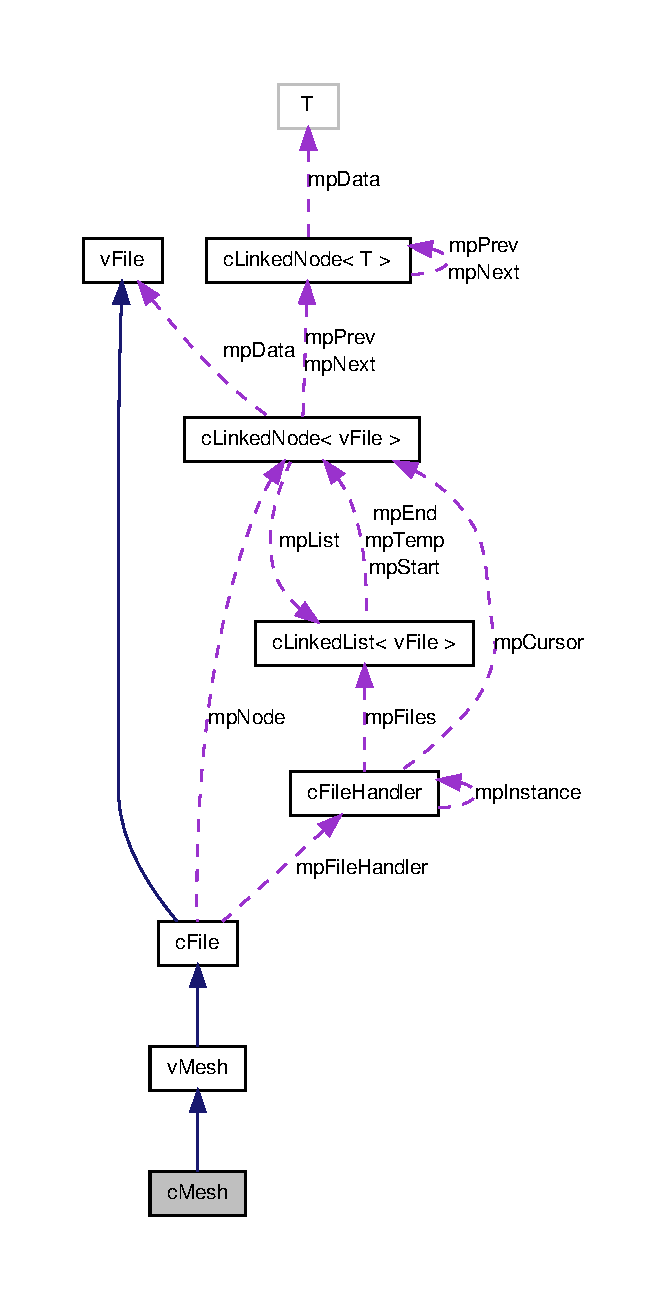
\includegraphics[width=325pt]{classc_mesh__coll__graph}
\end{center}
\end{figure}
\subsection*{Public Member Functions}
\begin{DoxyCompactItemize}
\item 
\hypertarget{classc_mesh_a1b689b9d00f34fe7e4cbf8910bb310f9}{
\hyperlink{classc_mesh_a1b689b9d00f34fe7e4cbf8910bb310f9}{cMesh} ()}
\label{classc_mesh_a1b689b9d00f34fe7e4cbf8910bb310f9}

\begin{DoxyCompactList}\small\item\em This will create an empty mesh. No verteces, no faces, nothing. \end{DoxyCompactList}\item 
\hypertarget{classc_mesh_ae24161941f8538d55caa144d76b535bc}{
\hyperlink{classc_mesh_ae24161941f8538d55caa144d76b535bc}{cMesh} (\hyperlink{classc_mesh_array}{cMeshArray} $\ast$lpMesh)}
\label{classc_mesh_ae24161941f8538d55caa144d76b535bc}

\begin{DoxyCompactList}\small\item\em This will load the data in lpMesh to be used by this object. \end{DoxyCompactList}\item 
\hypertarget{classc_mesh_a8dd2a8840d8e2c6aaefa95884a2f9f68}{
void \hyperlink{classc_mesh_a8dd2a8840d8e2c6aaefa95884a2f9f68}{SetFormat} ()}
\label{classc_mesh_a8dd2a8840d8e2c6aaefa95884a2f9f68}

\begin{DoxyCompactList}\small\item\em This will return the models rendering format. \end{DoxyCompactList}\item 
\hypertarget{classc_mesh_a5f35c2b9245d765b7958f91379d63e7d}{
void \hyperlink{classc_mesh_a5f35c2b9245d765b7958f91379d63e7d}{CreateNormalArray} ()}
\label{classc_mesh_a5f35c2b9245d765b7958f91379d63e7d}

\begin{DoxyCompactList}\small\item\em This will produce an array of vertex normal data for a mesh. This will require the mesh to have vertex and face data and produces normal vectors for all the verteces. \end{DoxyCompactList}\item 
\hypertarget{classc_mesh_a13513f988b641fb082e6e00d1e6c64e2}{
uint32 \hyperlink{classc_mesh_a13513f988b641fb082e6e00d1e6c64e2}{Verteces} ()}
\label{classc_mesh_a13513f988b641fb082e6e00d1e6c64e2}

\begin{DoxyCompactList}\small\item\em This will return the number of verteces in the vertex position array mpVertex. \end{DoxyCompactList}\item 
\hypertarget{classc_mesh_a5f1b578685730d581301f3b5dbb2f83c}{
uint32 \hyperlink{classc_mesh_a5f1b578685730d581301f3b5dbb2f83c}{Faces} ()}
\label{classc_mesh_a5f1b578685730d581301f3b5dbb2f83c}

\begin{DoxyCompactList}\small\item\em This will return the number of faces in the face array mpFaces. \end{DoxyCompactList}\item 
\hypertarget{classc_mesh_a56283d0c69f6b4987176c8714eb10987}{
float $\ast$ \hyperlink{classc_mesh_a56283d0c69f6b4987176c8714eb10987}{VertexData} ()}
\label{classc_mesh_a56283d0c69f6b4987176c8714eb10987}

\begin{DoxyCompactList}\small\item\em This will return a pointer to the vertex position array. \end{DoxyCompactList}\item 
\hypertarget{classc_mesh_a6bc80e837d5556b84399065c9a21fa79}{
FACE\_\-TYPE $\ast$ \hyperlink{classc_mesh_a6bc80e837d5556b84399065c9a21fa79}{FaceData} ()}
\label{classc_mesh_a6bc80e837d5556b84399065c9a21fa79}

\begin{DoxyCompactList}\small\item\em This will return a pointer to the face array.. \end{DoxyCompactList}\item 
\hypertarget{classc_mesh_a534e2fc01c1ed2319d067cdb2df0c439}{
float $\ast$ \hyperlink{classc_mesh_a534e2fc01c1ed2319d067cdb2df0c439}{NormalData} ()}
\label{classc_mesh_a534e2fc01c1ed2319d067cdb2df0c439}

\begin{DoxyCompactList}\small\item\em This will return a pointer to the array of vertex normals. \end{DoxyCompactList}\item 
\hypertarget{classc_mesh_a98e9d13a984398ecbe18300d435d01d8}{
float $\ast$ \hyperlink{classc_mesh_a98e9d13a984398ecbe18300d435d01d8}{UVData} ()}
\label{classc_mesh_a98e9d13a984398ecbe18300d435d01d8}

\begin{DoxyCompactList}\small\item\em This will return a pointer to the array of texture co-\/ordinates. \end{DoxyCompactList}\item 
\hypertarget{classc_mesh_a022d36f1b2f456b5edb50d32956960e0}{
void \hyperlink{classc_mesh_a022d36f1b2f456b5edb50d32956960e0}{Position} (float lfX, float lfY, float lfZ)}
\label{classc_mesh_a022d36f1b2f456b5edb50d32956960e0}

\begin{DoxyCompactList}\small\item\em This will move the objects centre of rotation by lfX,lfY,lfZ. \end{DoxyCompactList}\item 
\hypertarget{classc_mesh_a4d0f5cbdb12f1bc7fb8899c61d2328d5}{
void \hyperlink{classc_mesh_a4d0f5cbdb12f1bc7fb8899c61d2328d5}{PositionX} (float lfX)}
\label{classc_mesh_a4d0f5cbdb12f1bc7fb8899c61d2328d5}

\begin{DoxyCompactList}\small\item\em This will move the objects centre of rotation along its X axis lfX distance. \end{DoxyCompactList}\item 
\hypertarget{classc_mesh_a031dd39f3c8aa1643a978b42bfc68ddc}{
void \hyperlink{classc_mesh_a031dd39f3c8aa1643a978b42bfc68ddc}{PositionY} (float lfY)}
\label{classc_mesh_a031dd39f3c8aa1643a978b42bfc68ddc}

\begin{DoxyCompactList}\small\item\em This will move the objects centre of rotation along its Y axis lfY distance. \end{DoxyCompactList}\item 
\hypertarget{classc_mesh_a75062dccdd861877dd206f81ac2f9ec0}{
void \hyperlink{classc_mesh_a75062dccdd861877dd206f81ac2f9ec0}{PositionZ} (float lfZ)}
\label{classc_mesh_a75062dccdd861877dd206f81ac2f9ec0}

\begin{DoxyCompactList}\small\item\em This will move the objects centre of rotation along its Z axis lfZ distance. \end{DoxyCompactList}\item 
\hypertarget{classc_mesh_a6b4d72718fa9a90fae3ee30dbe5f2575}{
void \hyperlink{classc_mesh_a6b4d72718fa9a90fae3ee30dbe5f2575}{ResetPosition} ()}
\label{classc_mesh_a6b4d72718fa9a90fae3ee30dbe5f2575}

\begin{DoxyCompactList}\small\item\em This will restore the objects original centre of rotation. \end{DoxyCompactList}\item 
\hypertarget{classc_mesh_a93bdde998cfebc274b7573444dc98d34}{
float \hyperlink{classc_mesh_a93bdde998cfebc274b7573444dc98d34}{GetSize} ()}
\label{classc_mesh_a93bdde998cfebc274b7573444dc98d34}

\begin{DoxyCompactList}\small\item\em This will return the size of the Mesh. Size being the radius of the sphere required to contain the \hyperlink{classc_mesh}{cMesh} object. \end{DoxyCompactList}\item 
\hypertarget{classc_mesh_a47b1bea169448ce42035a82115a6ac48}{
double \hyperlink{classc_mesh_a47b1bea169448ce42035a82115a6ac48}{GetSizeSq} ()}
\label{classc_mesh_a47b1bea169448ce42035a82115a6ac48}

\begin{DoxyCompactList}\small\item\em This will return the size of the Mesh squared. Size being the radius of the sphere required to contain the \hyperlink{classc_mesh}{cMesh} object. \end{DoxyCompactList}\item 
\hypertarget{classc_mesh_abaa10891ab82ca5988bb255fda7cfdae}{
void \hyperlink{classc_mesh_abaa10891ab82ca5988bb255fda7cfdae}{FindSize} ()}
\label{classc_mesh_abaa10891ab82ca5988bb255fda7cfdae}

\begin{DoxyCompactList}\small\item\em This will calculate the size of the Mesh. Size being the radius of the sphere required to contain the \hyperlink{classc_mesh}{cMesh} object. \end{DoxyCompactList}\item 
\hypertarget{classc_mesh_ad3532e19ca542f90797df565b10c2be5}{
c2DVf \hyperlink{classc_mesh_ad3532e19ca542f90797df565b10c2be5}{FindUVCoordinates} (c3DVf ModelPos, float $\ast$lpTangent, float $\ast$lpBinormal, float $\ast$NormalData)}
\label{classc_mesh_ad3532e19ca542f90797df565b10c2be5}

\begin{DoxyCompactList}\small\item\em This will return the closest UV co-\/ordinates to a point in Model Space. Requires TBN Data. \end{DoxyCompactList}\item 
\hypertarget{classc_mesh_a325c1397e0594d3b19b11e4f789f93ca}{
\hyperlink{classc_mesh}{cMesh} $\ast$ \hyperlink{classc_mesh_a325c1397e0594d3b19b11e4f789f93ca}{Duplicate} (string lsFileName=\char`\"{}\char`\"{})}
\label{classc_mesh_a325c1397e0594d3b19b11e4f789f93ca}

\begin{DoxyCompactList}\small\item\em This will duplicate this mesh and return the pointer to the new instance. It can be named with lsFileName, if not it will be named \char`\"{}GeneratedMesh\char`\"{}. \end{DoxyCompactList}\item 
\hypertarget{classc_mesh_a637f8906a64eef54f320b59e8064a725}{
void \hyperlink{classc_mesh_a637f8906a64eef54f320b59e8064a725}{Equals} (\hyperlink{classc_mesh}{cMesh} $\ast$lpMesh, string lsFileName=\char`\"{}\char`\"{})}
\label{classc_mesh_a637f8906a64eef54f320b59e8064a725}

\begin{DoxyCompactList}\small\item\em This will make this \hyperlink{classc_mesh}{cMesh} duplicate lpMesh. It can be named with lsFileName, if not it will be named \char`\"{}GeneratedMesh\char`\"{}. \end{DoxyCompactList}\end{DoxyCompactItemize}
\subsection*{Protected Attributes}
\begin{DoxyCompactItemize}
\item 
\hypertarget{classc_mesh_a6a9c96e41eef3faed3c43ab69e8be5c6}{
uint8 \hyperlink{classc_mesh_a6a9c96e41eef3faed3c43ab69e8be5c6}{miFormat}}
\label{classc_mesh_a6a9c96e41eef3faed3c43ab69e8be5c6}

\begin{DoxyCompactList}\small\item\em This stores the format which determines what data is used to render the model. The flags in this variable determine what data is present to be used by the renderer $\ast$ relative to this object. see flags WT\_\-MESH\_\-FORMAT\_\-VERTECES, WT\_\-MESH\_\-FORMAT\_\-UVS, WT\_\-MESH\_\-FORMAT\_\-NORMALS and WT\_\-MESH\_\-FORMAT\_\-POSITIVE. \end{DoxyCompactList}\end{DoxyCompactItemize}


\subsection{Detailed Description}
This class stores the data for a 3D model. 


\begin{DoxyParams}{Parameters}
{\em lpMesh} & This is a pointer to a \hyperlink{classc_mesh_array}{cMeshArray} object which holds the mesh data for this object. This holds the data for a 3D model in a format suitable for rendering. The data is stored in 2 large arrays with the face data stored in the array mpFaces while all the remaining data stored is stored consecutively in mpVertex. mpVertex points to the start of the array while mpNormals and mpUV point to the start of their respective data blocks. \\
\hline
\end{DoxyParams}

\hypertarget{classc_mesh_array}{
\section{cMeshArray Class Reference}
\label{classc_mesh_array}\index{cMeshArray@{cMeshArray}}
}


This is a temporary storage class to ease transformation of data from the hdd to the \hyperlink{classc_mesh}{cMesh} class.  




Inheritance diagram for cMeshArray:
\nopagebreak
\begin{figure}[H]
\begin{center}
\leavevmode
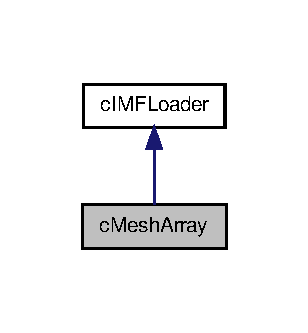
\includegraphics[width=148pt]{classc_mesh_array__inherit__graph}
\end{center}
\end{figure}


Collaboration diagram for cMeshArray:
\nopagebreak
\begin{figure}[H]
\begin{center}
\leavevmode
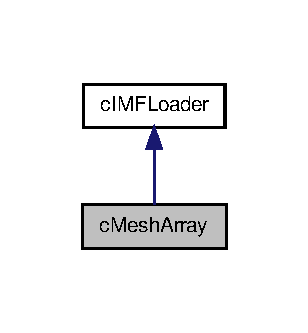
\includegraphics[width=148pt]{classc_mesh_array__coll__graph}
\end{center}
\end{figure}
\subsection*{Public Member Functions}
\begin{DoxyCompactItemize}
\item 
\hyperlink{classc_mesh_array_a7f8a0a0053d2a91d5c91bed80ec745ee}{cMeshArray} ()
\item 
void \hyperlink{classc_mesh_array_adce4a1c4b77569227f23d1e4cc46b4bb}{LoadIMF} (ifstream \&FileStream)
\begin{DoxyCompactList}\small\item\em This will load the data from an IMF File. \item\end{DoxyCompactList}\item 
\hyperlink{classc_mesh_array_a142887dc3853e28068cd0ad89aed926c}{$\sim$cMeshArray} ()
\end{DoxyCompactItemize}
\subsection*{Public Attributes}
\begin{DoxyCompactItemize}
\item 
float $\ast$ \hyperlink{classc_mesh_array_a4dce50ad6de11940afa0af53fdcefc27}{mpVertex}
\item 
float $\ast$ \hyperlink{classc_mesh_array_a1c568717706de37f77729a9292ceee42}{mpNormals}
\item 
float $\ast$ \hyperlink{classc_mesh_array_a9119e5c042443437ac22f06775662d4d}{mpUV}
\item 
uint16 $\ast$ \hyperlink{classc_mesh_array_aab7e25f0aaf4c7afb2dd0f0384867766}{mpFaces}
\item 
uint32 \hyperlink{classc_mesh_array_a340440f28957f97372571295422880b3}{miVertex}
\item 
uint32 \hyperlink{classc_mesh_array_ad1fa1c6dbc63102948626412a90cf117}{miFaces}
\item 
char $\ast$ \hyperlink{classc_mesh_array_a31b40f14b026b9957f4ae44b58565061}{mpRef}
\end{DoxyCompactItemize}


\subsection{Detailed Description}
This is a temporary storage class to ease transformation of data from the hdd to the \hyperlink{classc_mesh}{cMesh} class. 

Definition at line 14 of file WTcMesh.h.



\subsection{Constructor \& Destructor Documentation}
\hypertarget{classc_mesh_array_a7f8a0a0053d2a91d5c91bed80ec745ee}{
\index{cMeshArray@{cMeshArray}!cMeshArray@{cMeshArray}}
\index{cMeshArray@{cMeshArray}!cMeshArray@{cMeshArray}}
\subsubsection[{cMeshArray}]{\setlength{\rightskip}{0pt plus 5cm}cMeshArray::cMeshArray (
\begin{DoxyParamCaption}
{}
\end{DoxyParamCaption}
)}}
\label{classc_mesh_array_a7f8a0a0053d2a91d5c91bed80ec745ee}


Definition at line 48 of file WTcMesh.cpp.

\hypertarget{classc_mesh_array_a142887dc3853e28068cd0ad89aed926c}{
\index{cMeshArray@{cMeshArray}!$\sim$cMeshArray@{$\sim$cMeshArray}}
\index{$\sim$cMeshArray@{$\sim$cMeshArray}!cMeshArray@{cMeshArray}}
\subsubsection[{$\sim$cMeshArray}]{\setlength{\rightskip}{0pt plus 5cm}cMeshArray::$\sim$cMeshArray (
\begin{DoxyParamCaption}
{}
\end{DoxyParamCaption}
)}}
\label{classc_mesh_array_a142887dc3853e28068cd0ad89aed926c}


Definition at line 53 of file WTcMesh.cpp.



\subsection{Member Function Documentation}
\hypertarget{classc_mesh_array_adce4a1c4b77569227f23d1e4cc46b4bb}{
\index{cMeshArray@{cMeshArray}!LoadIMF@{LoadIMF}}
\index{LoadIMF@{LoadIMF}!cMeshArray@{cMeshArray}}
\subsubsection[{LoadIMF}]{\setlength{\rightskip}{0pt plus 5cm}void cMeshArray::LoadIMF (
\begin{DoxyParamCaption}
\item[{ifstream \&}]{FileStream}
\end{DoxyParamCaption}
)}}
\label{classc_mesh_array_adce4a1c4b77569227f23d1e4cc46b4bb}


This will load the data from an IMF File. 



Reimplemented from \hyperlink{classc_i_m_f_loader_a219c95a2cfbb5f477b10d9158f77470c}{cIMFLoader}.



Definition at line 3 of file WTcMesh.cpp.



\subsection{Member Data Documentation}
\hypertarget{classc_mesh_array_ad1fa1c6dbc63102948626412a90cf117}{
\index{cMeshArray@{cMeshArray}!miFaces@{miFaces}}
\index{miFaces@{miFaces}!cMeshArray@{cMeshArray}}
\subsubsection[{miFaces}]{\setlength{\rightskip}{0pt plus 5cm}uint32 {\bf cMeshArray::miFaces}}}
\label{classc_mesh_array_ad1fa1c6dbc63102948626412a90cf117}


Definition at line 29 of file WTcMesh.h.

\hypertarget{classc_mesh_array_a340440f28957f97372571295422880b3}{
\index{cMeshArray@{cMeshArray}!miVertex@{miVertex}}
\index{miVertex@{miVertex}!cMeshArray@{cMeshArray}}
\subsubsection[{miVertex}]{\setlength{\rightskip}{0pt plus 5cm}uint32 {\bf cMeshArray::miVertex}}}
\label{classc_mesh_array_a340440f28957f97372571295422880b3}


Definition at line 27 of file WTcMesh.h.

\hypertarget{classc_mesh_array_aab7e25f0aaf4c7afb2dd0f0384867766}{
\index{cMeshArray@{cMeshArray}!mpFaces@{mpFaces}}
\index{mpFaces@{mpFaces}!cMeshArray@{cMeshArray}}
\subsubsection[{mpFaces}]{\setlength{\rightskip}{0pt plus 5cm}uint16$\ast$ {\bf cMeshArray::mpFaces}}}
\label{classc_mesh_array_aab7e25f0aaf4c7afb2dd0f0384867766}


Definition at line 25 of file WTcMesh.h.

\hypertarget{classc_mesh_array_a1c568717706de37f77729a9292ceee42}{
\index{cMeshArray@{cMeshArray}!mpNormals@{mpNormals}}
\index{mpNormals@{mpNormals}!cMeshArray@{cMeshArray}}
\subsubsection[{mpNormals}]{\setlength{\rightskip}{0pt plus 5cm}float$\ast$ {\bf cMeshArray::mpNormals}}}
\label{classc_mesh_array_a1c568717706de37f77729a9292ceee42}


Definition at line 21 of file WTcMesh.h.

\hypertarget{classc_mesh_array_a31b40f14b026b9957f4ae44b58565061}{
\index{cMeshArray@{cMeshArray}!mpRef@{mpRef}}
\index{mpRef@{mpRef}!cMeshArray@{cMeshArray}}
\subsubsection[{mpRef}]{\setlength{\rightskip}{0pt plus 5cm}char$\ast$ {\bf cMeshArray::mpRef}}}
\label{classc_mesh_array_a31b40f14b026b9957f4ae44b58565061}


Definition at line 31 of file WTcMesh.h.

\hypertarget{classc_mesh_array_a9119e5c042443437ac22f06775662d4d}{
\index{cMeshArray@{cMeshArray}!mpUV@{mpUV}}
\index{mpUV@{mpUV}!cMeshArray@{cMeshArray}}
\subsubsection[{mpUV}]{\setlength{\rightskip}{0pt plus 5cm}float$\ast$ {\bf cMeshArray::mpUV}}}
\label{classc_mesh_array_a9119e5c042443437ac22f06775662d4d}


Definition at line 23 of file WTcMesh.h.

\hypertarget{classc_mesh_array_a4dce50ad6de11940afa0af53fdcefc27}{
\index{cMeshArray@{cMeshArray}!mpVertex@{mpVertex}}
\index{mpVertex@{mpVertex}!cMeshArray@{cMeshArray}}
\subsubsection[{mpVertex}]{\setlength{\rightskip}{0pt plus 5cm}float$\ast$ {\bf cMeshArray::mpVertex}}}
\label{classc_mesh_array_a4dce50ad6de11940afa0af53fdcefc27}


Definition at line 19 of file WTcMesh.h.


\hypertarget{classc_mesh_collision}{
\section{cMeshCollision Class Reference}
\label{classc_mesh_collision}\index{cMeshCollision@{cMeshCollision}}
}


Collaboration diagram for cMeshCollision:\nopagebreak
\begin{figure}[H]
\begin{center}
\leavevmode
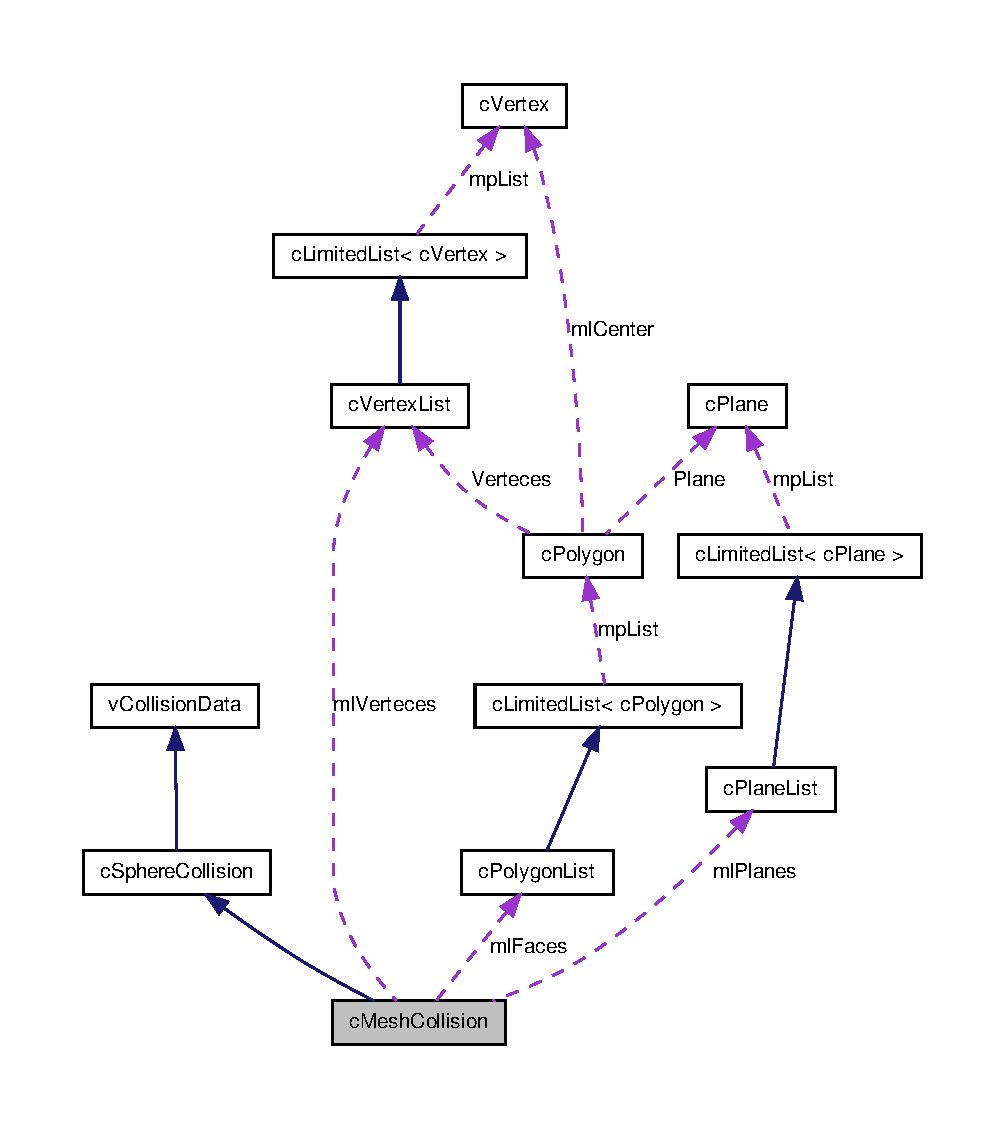
\includegraphics[width=400pt]{classc_mesh_collision__coll__graph}
\end{center}
\end{figure}
\subsection*{Public Member Functions}
\begin{DoxyCompactItemize}
\item 
void \hyperlink{classc_mesh_collision_a49a69f58cf68f61f995119c077c26a75}{BuildObject} (float $\ast$lpRanges)
\item 
\hypertarget{classc_mesh_collision_a861e58e0eacea406250fa1eef10c9860}{
\hyperlink{classc_mesh_collision}{cMeshCollision} $\ast$ \hyperlink{classc_mesh_collision_a861e58e0eacea406250fa1eef10c9860}{Mesh} ()}
\label{classc_mesh_collision_a861e58e0eacea406250fa1eef10c9860}

\begin{DoxyCompactList}\small\item\em Will return a pointer if this object contains a Mesh collision data object. Otherwise returns 0;. \end{DoxyCompactList}\item 
\hypertarget{classc_mesh_collision_accad5d32a30bb6fe79df75f1702125fd}{
uint8 \hyperlink{classc_mesh_collision_accad5d32a30bb6fe79df75f1702125fd}{Type} ()}
\label{classc_mesh_collision_accad5d32a30bb6fe79df75f1702125fd}

\begin{DoxyCompactList}\small\item\em Will return the Objects Type. \end{DoxyCompactList}\end{DoxyCompactItemize}


\subsection{Detailed Description}
This is the cCollisionData class for Boxes. Boxes can either be loaded from a file or procedurally generated. These boxes actually work as simple Collision Meshes with 6 planes and 8 verteces. Will Rotate as object moves. 

\subsection{Member Function Documentation}
\hypertarget{classc_mesh_collision_a49a69f58cf68f61f995119c077c26a75}{
\index{cMeshCollision@{cMeshCollision}!BuildObject@{BuildObject}}
\index{BuildObject@{BuildObject}!cMeshCollision@{cMeshCollision}}
\subsubsection[{BuildObject}]{\setlength{\rightskip}{0pt plus 5cm}void cMeshCollision::BuildObject (
\begin{DoxyParamCaption}
\item[{float $\ast$}]{lpRanges}
\end{DoxyParamCaption}
)}}
\label{classc_mesh_collision_a49a69f58cf68f61f995119c077c26a75}
This will build a Box collision. Expects an array of 6 float values representing the length of the normal vector for each plane. (-\/X, +X, -\/Y, +Y, -\/Z, +Z). Floats passed to this function which are +ve will produce a plane facing away from 0,0,0 (origin is behind the plane). Floats passed to this function which are -\/ve will produce a plane facing towards 0,0,0 (origin is in front of the plane). This way boxes can be constructed which do not contain the origin. 
\hypertarget{classc_mesh_file_collision}{
\section{cMeshFileCollision Class Reference}
\label{classc_mesh_file_collision}\index{cMeshFileCollision@{cMeshFileCollision}}
}


Mesh Collision Object with functionality to load a Collision Mesh from a file. This inherits \hyperlink{classc_mesh_collision}{cMeshCollision}, so uses that code for defining the Mesh Collision Object.  




Collaboration diagram for cMeshFileCollision:\nopagebreak
\begin{figure}[H]
\begin{center}
\leavevmode
\includegraphics[width=400pt]{classc_mesh_file_collision__coll__graph}
\end{center}
\end{figure}
\subsection*{Public Member Functions}
\begin{DoxyCompactItemize}
\item 
\hypertarget{classc_mesh_file_collision_ac40c927ae3dfecfb2c9a0e40fbcd31b3}{
void \hyperlink{classc_mesh_file_collision_ac40c927ae3dfecfb2c9a0e40fbcd31b3}{LoadIMF} (ifstream \&FileStream)}
\label{classc_mesh_file_collision_ac40c927ae3dfecfb2c9a0e40fbcd31b3}

\begin{DoxyCompactList}\small\item\em Will Load a Collision Mesh Object from an IMF File. \end{DoxyCompactList}\end{DoxyCompactItemize}


\subsection{Detailed Description}
Mesh Collision Object with functionality to load a Collision Mesh from a file. This inherits \hyperlink{classc_mesh_collision}{cMeshCollision}, so uses that code for defining the Mesh Collision Object. 


\hypertarget{classc_mesh_tree}{
\section{cMeshTree Class Reference}
\label{classc_mesh_tree}\index{cMeshTree@{cMeshTree}}
}


This will store the data for a cModelList()  




Collaboration diagram for cMeshTree:\nopagebreak
\begin{figure}[H]
\begin{center}
\leavevmode
\includegraphics[height=600pt]{classc_mesh_tree__coll__graph}
\end{center}
\end{figure}
\subsection*{Public Member Functions}
\begin{DoxyCompactItemize}
\item 
\hypertarget{classc_mesh_tree_a5847e3ca4f4f2531c6b0df1cd2c7a783}{
\hyperlink{classc_mesh_tree_a5847e3ca4f4f2531c6b0df1cd2c7a783}{cMeshTree} (\hyperlink{classc_mesh_tree_array}{cMeshTreeArray} $\ast$lpArray)}
\label{classc_mesh_tree_a5847e3ca4f4f2531c6b0df1cd2c7a783}

\begin{DoxyCompactList}\small\item\em This will extract the data from the cMeshTreeArray() lpArray. \end{DoxyCompactList}\item 
\hypertarget{classc_mesh_tree_af3667772e99dbbff048fc5189af7cf07}{
uint32 \hyperlink{classc_mesh_tree_af3667772e99dbbff048fc5189af7cf07}{TreeSize} ()}
\label{classc_mesh_tree_af3667772e99dbbff048fc5189af7cf07}

\begin{DoxyCompactList}\small\item\em This is actually the length of the Tree. \end{DoxyCompactList}\item 
\hypertarget{classc_mesh_tree_a2af67ab77feaed272985daf8b74ed662}{
\hyperlink{classc_mesh_tree_node}{cMeshTreeNode} $\ast$ \hyperlink{classc_mesh_tree_a2af67ab77feaed272985daf8b74ed662}{NodeList} ()}
\label{classc_mesh_tree_a2af67ab77feaed272985daf8b74ed662}

\begin{DoxyCompactList}\small\item\em This will return a pointer to the first item of mpList. \end{DoxyCompactList}\item 
\hypertarget{classc_mesh_tree_ae7545034b95adcf5e2f77fb009ffd803}{
\hyperlink{classc_mesh_tree_node}{cMeshTreeNode} $\ast$ \hyperlink{classc_mesh_tree_ae7545034b95adcf5e2f77fb009ffd803}{NodeList} (uint32 liCount)}
\label{classc_mesh_tree_ae7545034b95adcf5e2f77fb009ffd803}

\begin{DoxyCompactList}\small\item\em This will return a pointer to the \hyperlink{classc_mesh_tree_node}{cMeshTreeNode} in position liCount in mpList. \end{DoxyCompactList}\item 
\hypertarget{classc_mesh_tree_a3c82682fe2453aed6c5cdcf0316894bd}{
float \hyperlink{classc_mesh_tree_a3c82682fe2453aed6c5cdcf0316894bd}{GetSize} ()}
\label{classc_mesh_tree_a3c82682fe2453aed6c5cdcf0316894bd}

\begin{DoxyCompactList}\small\item\em This will return the spatial size of this \hyperlink{classc_mesh_tree_a5847e3ca4f4f2531c6b0df1cd2c7a783}{cMeshTree()} \end{DoxyCompactList}\item 
\hypertarget{classc_mesh_tree_a66008bdef8db37c172502b0c7de87e31}{
float \hyperlink{classc_mesh_tree_a66008bdef8db37c172502b0c7de87e31}{FindSize} ()}
\label{classc_mesh_tree_a66008bdef8db37c172502b0c7de87e31}

\begin{DoxyCompactList}\small\item\em This will calculate the spatial size of this \hyperlink{classc_mesh_tree_a5847e3ca4f4f2531c6b0df1cd2c7a783}{cMeshTree()} \end{DoxyCompactList}\end{DoxyCompactItemize}


\subsection{Detailed Description}
This will store the data for a cModelList() 
\hypertarget{classc_mesh_tree_array}{
\section{cMeshTreeArray Class Reference}
\label{classc_mesh_tree_array}\index{cMeshTreeArray@{cMeshTreeArray}}
}


This will load the information from an IMF file to be handed to a cMeshTree() This object will store the data for a cMeshTree() object from an IMF file.  




Collaboration diagram for cMeshTreeArray:\nopagebreak
\begin{figure}[H]
\begin{center}
\leavevmode
\includegraphics[width=400pt]{classc_mesh_tree_array__coll__graph}
\end{center}
\end{figure}
\subsection*{Public Member Functions}
\begin{DoxyCompactItemize}
\item 
\hypertarget{classc_mesh_tree_array_af8f0a2e58b086a46e5dd12aca2310377}{
\hyperlink{classc_mesh_tree_array_af8f0a2e58b086a46e5dd12aca2310377}{cMeshTreeArray} ()}
\label{classc_mesh_tree_array_af8f0a2e58b086a46e5dd12aca2310377}

\begin{DoxyCompactList}\small\item\em This is a public constructor, it will initialise the data for this class. \end{DoxyCompactList}\item 
\hypertarget{classc_mesh_tree_array_a98917f5d6920454275acf420d78e3f25}{
\hyperlink{classc_mesh_tree_array_a98917f5d6920454275acf420d78e3f25}{$\sim$cMeshTreeArray} ()}
\label{classc_mesh_tree_array_a98917f5d6920454275acf420d78e3f25}

\begin{DoxyCompactList}\small\item\em This is a public deconstructor. \end{DoxyCompactList}\end{DoxyCompactItemize}
\subsection*{Public Attributes}
\begin{DoxyCompactItemize}
\item 
\hypertarget{classc_mesh_tree_array_a83f4ee5f93ed62e7f939eed3b5e68cda}{
\hyperlink{classc_mesh_tree_node}{cMeshTreeNode} $\ast$ \hyperlink{classc_mesh_tree_array_a83f4ee5f93ed62e7f939eed3b5e68cda}{mpList}}
\label{classc_mesh_tree_array_a83f4ee5f93ed62e7f939eed3b5e68cda}

\begin{DoxyCompactList}\small\item\em This will point to an array of cMeshTreeNode() objects. \end{DoxyCompactList}\item 
\hypertarget{classc_mesh_tree_array_a23d238161a175633f64af87a2bc85984}{
uint32 \hyperlink{classc_mesh_tree_array_a23d238161a175633f64af87a2bc85984}{miTreeLength}}
\label{classc_mesh_tree_array_a23d238161a175633f64af87a2bc85984}

\begin{DoxyCompactList}\small\item\em This is the number of cMeshTreeNode() objects in the tree. \end{DoxyCompactList}\item 
\hypertarget{classc_mesh_tree_array_a1114b12bb1a849122403e0d2e1fb2ec6}{
char $\ast$ \hyperlink{classc_mesh_tree_array_a1114b12bb1a849122403e0d2e1fb2ec6}{mpRef}}
\label{classc_mesh_tree_array_a1114b12bb1a849122403e0d2e1fb2ec6}

\begin{DoxyCompactList}\small\item\em This will point to an array storing the string reference for this object. \end{DoxyCompactList}\end{DoxyCompactItemize}


\subsection{Detailed Description}
This will load the information from an IMF file to be handed to a cMeshTree() This object will store the data for a cMeshTree() object from an IMF file. 
\hypertarget{classc_mesh_tree_node}{
\section{cMeshTreeNode Class Reference}
\label{classc_mesh_tree_node}\index{cMeshTreeNode@{cMeshTreeNode}}
}


This object will store the data for a single item in a cMeshTree(). This stores the Position, Rotation, Mesh, Texture, Tree Level, for this object.  




Collaboration diagram for cMeshTreeNode:
\nopagebreak
\begin{figure}[H]
\begin{center}
\leavevmode
\includegraphics[height=600pt]{classc_mesh_tree_node__coll__graph}
\end{center}
\end{figure}
\subsection*{Public Member Functions}
\begin{DoxyCompactItemize}
\item 
\hyperlink{classc_mesh_tree_node_aa0506651f17427bfdbababeb406eb8f3}{cMeshTreeNode} ()
\item 
\hyperlink{classc_mesh_tree_node_a6879af803641d312d8ba07d5361198b3}{$\sim$cMeshTreeNode} ()
\item 
void \hyperlink{classc_mesh_tree_node_a043efc30a09c9a474d75b7c5e79abccc}{Initialise} ()
\begin{DoxyCompactList}\small\item\em This will Initialise the objects data. \item\end{DoxyCompactList}\item 
void \hyperlink{classc_mesh_tree_node_ac75b9a8974308873997ad6fcc5baa0da}{RemoveMesh} ()
\begin{DoxyCompactList}\small\item\em This will Remove and Delete the Mesh. \item\end{DoxyCompactList}\item 
void \hyperlink{classc_mesh_tree_node_ab3c5c436df69d8f6ef8a5348e76f5784}{RemoveTexture} ()
\begin{DoxyCompactList}\small\item\em This will Remove and Delete the Texture. \item\end{DoxyCompactList}\item 
void \hyperlink{classc_mesh_tree_node_a289e7a882f0304a0e2738a7cca5db60d}{RemoveStackLevel} ()
\begin{DoxyCompactList}\small\item\em This will reset the Tree Level. \item\end{DoxyCompactList}\item 
void \hyperlink{classc_mesh_tree_node_ad9659fb0be5e1300bcda2265d651dd97}{RemovePosition} ()
\begin{DoxyCompactList}\small\item\em This will Reset the Position. \item\end{DoxyCompactList}\item 
void \hyperlink{classc_mesh_tree_node_a9ea8fa642a22c047b2e6d559976b615b}{RemoveRotation} ()
\begin{DoxyCompactList}\small\item\em This will Reset the Rotation. \item\end{DoxyCompactList}\item 
void \hyperlink{classc_mesh_tree_node_a1ca09fa05700321ca076d327fa99220b}{ReadIMF} (ifstream \&FileStream)
\begin{DoxyCompactList}\small\item\em This will Load a \hyperlink{classc_mesh_tree_node_aa0506651f17427bfdbababeb406eb8f3}{cMeshTreeNode()} from an IMF File. FileStream should just have reached the start of the Mesh Tree Node. \item\end{DoxyCompactList}\item 
\hyperlink{classv_mesh}{vMesh} $\ast$ \hyperlink{classc_mesh_tree_node_a3056c26a6ce6ba8565dccef3ea15f5b5}{Mesh} ()
\begin{DoxyCompactList}\small\item\em This will return the Mesh for this object. \item\end{DoxyCompactList}\item 
\hyperlink{classv_texture}{vTexture} $\ast$ \hyperlink{classc_mesh_tree_node_ac0f2bde8c7a25e243841f6b4edcdeb82}{Texture} ()
\begin{DoxyCompactList}\small\item\em This will return the Texture for this object. \item\end{DoxyCompactList}\item 
float \hyperlink{classc_mesh_tree_node_a9e00261118c3ed9076abc38907a2e8d3}{GetSize} ()
\begin{DoxyCompactList}\small\item\em This will return the Spatial Size for this object. \item\end{DoxyCompactList}\end{DoxyCompactItemize}
\subsection*{Public Attributes}
\begin{DoxyCompactItemize}
\item 
uint32 \hyperlink{classc_mesh_tree_node_acba14d5e2688149f7891ea14816392d2}{miFormat}
\item 
char $\ast$ \hyperlink{classc_mesh_tree_node_af94ac50e58c5d1b29f7d971746d2b217}{mpMesh}
\item 
\hyperlink{classv_mesh}{vMesh} $\ast$ \hyperlink{classc_mesh_tree_node_a5207bf917599f81dcdd19877876a3987}{mpMeshPoint}
\item 
char $\ast$ \hyperlink{classc_mesh_tree_node_ade5fa05534442fd9a55a50741ddfd32e}{mpTexture}
\item 
\hyperlink{classv_texture}{vTexture} $\ast$ \hyperlink{classc_mesh_tree_node_a2c26ffbd7a3eade15a8e1943dc5eff40}{mpTexturePoint}
\item 
uint32 \hyperlink{classc_mesh_tree_node_a849588f1cad1d35030b1b7e148e5776b}{miLevel}
\item 
float $\ast$ \hyperlink{classc_mesh_tree_node_a70182df675cd9e665453177ff5959e92}{mpPosition}
\item 
float $\ast$ \hyperlink{classc_mesh_tree_node_a24e4bf28242619afb11daf82bd930a6d}{mpRotation}
\end{DoxyCompactItemize}


\subsection{Detailed Description}
This object will store the data for a single item in a cMeshTree(). This stores the Position, Rotation, Mesh, Texture, Tree Level, for this object. 

Definition at line 7 of file WTcMeshTreeNode.h.



\subsection{Constructor \& Destructor Documentation}
\hypertarget{classc_mesh_tree_node_aa0506651f17427bfdbababeb406eb8f3}{
\index{cMeshTreeNode@{cMeshTreeNode}!cMeshTreeNode@{cMeshTreeNode}}
\index{cMeshTreeNode@{cMeshTreeNode}!cMeshTreeNode@{cMeshTreeNode}}
\subsubsection[{cMeshTreeNode}]{\setlength{\rightskip}{0pt plus 5cm}cMeshTreeNode::cMeshTreeNode (
\begin{DoxyParamCaption}
{}
\end{DoxyParamCaption}
)}}
\label{classc_mesh_tree_node_aa0506651f17427bfdbababeb406eb8f3}


Definition at line 16 of file WTcMeshTreeNode.cpp.

\hypertarget{classc_mesh_tree_node_a6879af803641d312d8ba07d5361198b3}{
\index{cMeshTreeNode@{cMeshTreeNode}!$\sim$cMeshTreeNode@{$\sim$cMeshTreeNode}}
\index{$\sim$cMeshTreeNode@{$\sim$cMeshTreeNode}!cMeshTreeNode@{cMeshTreeNode}}
\subsubsection[{$\sim$cMeshTreeNode}]{\setlength{\rightskip}{0pt plus 5cm}cMeshTreeNode::$\sim$cMeshTreeNode (
\begin{DoxyParamCaption}
{}
\end{DoxyParamCaption}
)}}
\label{classc_mesh_tree_node_a6879af803641d312d8ba07d5361198b3}


Definition at line 21 of file WTcMeshTreeNode.cpp.



\subsection{Member Function Documentation}
\hypertarget{classc_mesh_tree_node_a9e00261118c3ed9076abc38907a2e8d3}{
\index{cMeshTreeNode@{cMeshTreeNode}!GetSize@{GetSize}}
\index{GetSize@{GetSize}!cMeshTreeNode@{cMeshTreeNode}}
\subsubsection[{GetSize}]{\setlength{\rightskip}{0pt plus 5cm}float cMeshTreeNode::GetSize (
\begin{DoxyParamCaption}
{}
\end{DoxyParamCaption}
)}}
\label{classc_mesh_tree_node_a9e00261118c3ed9076abc38907a2e8d3}


This will return the Spatial Size for this object. 



Definition at line 121 of file WTcMeshTreeNode.cpp.

\hypertarget{classc_mesh_tree_node_a043efc30a09c9a474d75b7c5e79abccc}{
\index{cMeshTreeNode@{cMeshTreeNode}!Initialise@{Initialise}}
\index{Initialise@{Initialise}!cMeshTreeNode@{cMeshTreeNode}}
\subsubsection[{Initialise}]{\setlength{\rightskip}{0pt plus 5cm}void cMeshTreeNode::Initialise (
\begin{DoxyParamCaption}
{}
\end{DoxyParamCaption}
)}}
\label{classc_mesh_tree_node_a043efc30a09c9a474d75b7c5e79abccc}


This will Initialise the objects data. 



Definition at line 6 of file WTcMeshTreeNode.cpp.

\hypertarget{classc_mesh_tree_node_a3056c26a6ce6ba8565dccef3ea15f5b5}{
\index{cMeshTreeNode@{cMeshTreeNode}!Mesh@{Mesh}}
\index{Mesh@{Mesh}!cMeshTreeNode@{cMeshTreeNode}}
\subsubsection[{Mesh}]{\setlength{\rightskip}{0pt plus 5cm}{\bf vMesh} $\ast$ cMeshTreeNode::Mesh (
\begin{DoxyParamCaption}
{}
\end{DoxyParamCaption}
)}}
\label{classc_mesh_tree_node_a3056c26a6ce6ba8565dccef3ea15f5b5}


This will return the Mesh for this object. 



Definition at line 98 of file WTcMeshTreeNode.cpp.

\hypertarget{classc_mesh_tree_node_a1ca09fa05700321ca076d327fa99220b}{
\index{cMeshTreeNode@{cMeshTreeNode}!ReadIMF@{ReadIMF}}
\index{ReadIMF@{ReadIMF}!cMeshTreeNode@{cMeshTreeNode}}
\subsubsection[{ReadIMF}]{\setlength{\rightskip}{0pt plus 5cm}void cMeshTreeNode::ReadIMF (
\begin{DoxyParamCaption}
\item[{ifstream \&}]{FileStream}
\end{DoxyParamCaption}
)}}
\label{classc_mesh_tree_node_a1ca09fa05700321ca076d327fa99220b}


This will Load a \hyperlink{classc_mesh_tree_node_aa0506651f17427bfdbababeb406eb8f3}{cMeshTreeNode()} from an IMF File. FileStream should just have reached the start of the Mesh Tree Node. 



Definition at line 48 of file WTcMeshTreeNode.cpp.

\hypertarget{classc_mesh_tree_node_ac75b9a8974308873997ad6fcc5baa0da}{
\index{cMeshTreeNode@{cMeshTreeNode}!RemoveMesh@{RemoveMesh}}
\index{RemoveMesh@{RemoveMesh}!cMeshTreeNode@{cMeshTreeNode}}
\subsubsection[{RemoveMesh}]{\setlength{\rightskip}{0pt plus 5cm}void cMeshTreeNode::RemoveMesh (
\begin{DoxyParamCaption}
{}
\end{DoxyParamCaption}
)}}
\label{classc_mesh_tree_node_ac75b9a8974308873997ad6fcc5baa0da}


This will Remove and Delete the Mesh. 



Definition at line 30 of file WTcMeshTreeNode.cpp.

\hypertarget{classc_mesh_tree_node_ad9659fb0be5e1300bcda2265d651dd97}{
\index{cMeshTreeNode@{cMeshTreeNode}!RemovePosition@{RemovePosition}}
\index{RemovePosition@{RemovePosition}!cMeshTreeNode@{cMeshTreeNode}}
\subsubsection[{RemovePosition}]{\setlength{\rightskip}{0pt plus 5cm}void cMeshTreeNode::RemovePosition (
\begin{DoxyParamCaption}
{}
\end{DoxyParamCaption}
)}}
\label{classc_mesh_tree_node_ad9659fb0be5e1300bcda2265d651dd97}


This will Reset the Position. 



Definition at line 41 of file WTcMeshTreeNode.cpp.

\hypertarget{classc_mesh_tree_node_a9ea8fa642a22c047b2e6d559976b615b}{
\index{cMeshTreeNode@{cMeshTreeNode}!RemoveRotation@{RemoveRotation}}
\index{RemoveRotation@{RemoveRotation}!cMeshTreeNode@{cMeshTreeNode}}
\subsubsection[{RemoveRotation}]{\setlength{\rightskip}{0pt plus 5cm}void cMeshTreeNode::RemoveRotation (
\begin{DoxyParamCaption}
{}
\end{DoxyParamCaption}
)}}
\label{classc_mesh_tree_node_a9ea8fa642a22c047b2e6d559976b615b}


This will Reset the Rotation. 



Definition at line 44 of file WTcMeshTreeNode.cpp.

\hypertarget{classc_mesh_tree_node_a289e7a882f0304a0e2738a7cca5db60d}{
\index{cMeshTreeNode@{cMeshTreeNode}!RemoveStackLevel@{RemoveStackLevel}}
\index{RemoveStackLevel@{RemoveStackLevel}!cMeshTreeNode@{cMeshTreeNode}}
\subsubsection[{RemoveStackLevel}]{\setlength{\rightskip}{0pt plus 5cm}void cMeshTreeNode::RemoveStackLevel (
\begin{DoxyParamCaption}
{}
\end{DoxyParamCaption}
)}}
\label{classc_mesh_tree_node_a289e7a882f0304a0e2738a7cca5db60d}


This will reset the Tree Level. 



Definition at line 36 of file WTcMeshTreeNode.cpp.

\hypertarget{classc_mesh_tree_node_ab3c5c436df69d8f6ef8a5348e76f5784}{
\index{cMeshTreeNode@{cMeshTreeNode}!RemoveTexture@{RemoveTexture}}
\index{RemoveTexture@{RemoveTexture}!cMeshTreeNode@{cMeshTreeNode}}
\subsubsection[{RemoveTexture}]{\setlength{\rightskip}{0pt plus 5cm}void cMeshTreeNode::RemoveTexture (
\begin{DoxyParamCaption}
{}
\end{DoxyParamCaption}
)}}
\label{classc_mesh_tree_node_ab3c5c436df69d8f6ef8a5348e76f5784}


This will Remove and Delete the Texture. 



Definition at line 33 of file WTcMeshTreeNode.cpp.

\hypertarget{classc_mesh_tree_node_ac0f2bde8c7a25e243841f6b4edcdeb82}{
\index{cMeshTreeNode@{cMeshTreeNode}!Texture@{Texture}}
\index{Texture@{Texture}!cMeshTreeNode@{cMeshTreeNode}}
\subsubsection[{Texture}]{\setlength{\rightskip}{0pt plus 5cm}{\bf vTexture} $\ast$ cMeshTreeNode::Texture (
\begin{DoxyParamCaption}
{}
\end{DoxyParamCaption}
)}}
\label{classc_mesh_tree_node_ac0f2bde8c7a25e243841f6b4edcdeb82}


This will return the Texture for this object. 



Definition at line 110 of file WTcMeshTreeNode.cpp.



\subsection{Member Data Documentation}
\hypertarget{classc_mesh_tree_node_acba14d5e2688149f7891ea14816392d2}{
\index{cMeshTreeNode@{cMeshTreeNode}!miFormat@{miFormat}}
\index{miFormat@{miFormat}!cMeshTreeNode@{cMeshTreeNode}}
\subsubsection[{miFormat}]{\setlength{\rightskip}{0pt plus 5cm}uint32 {\bf cMeshTreeNode::miFormat}}}
\label{classc_mesh_tree_node_acba14d5e2688149f7891ea14816392d2}


Definition at line 20 of file WTcMeshTreeNode.h.

\hypertarget{classc_mesh_tree_node_a849588f1cad1d35030b1b7e148e5776b}{
\index{cMeshTreeNode@{cMeshTreeNode}!miLevel@{miLevel}}
\index{miLevel@{miLevel}!cMeshTreeNode@{cMeshTreeNode}}
\subsubsection[{miLevel}]{\setlength{\rightskip}{0pt plus 5cm}uint32 {\bf cMeshTreeNode::miLevel}}}
\label{classc_mesh_tree_node_a849588f1cad1d35030b1b7e148e5776b}


Definition at line 25 of file WTcMeshTreeNode.h.

\hypertarget{classc_mesh_tree_node_af94ac50e58c5d1b29f7d971746d2b217}{
\index{cMeshTreeNode@{cMeshTreeNode}!mpMesh@{mpMesh}}
\index{mpMesh@{mpMesh}!cMeshTreeNode@{cMeshTreeNode}}
\subsubsection[{mpMesh}]{\setlength{\rightskip}{0pt plus 5cm}char$\ast$ {\bf cMeshTreeNode::mpMesh}}}
\label{classc_mesh_tree_node_af94ac50e58c5d1b29f7d971746d2b217}


Definition at line 21 of file WTcMeshTreeNode.h.

\hypertarget{classc_mesh_tree_node_a5207bf917599f81dcdd19877876a3987}{
\index{cMeshTreeNode@{cMeshTreeNode}!mpMeshPoint@{mpMeshPoint}}
\index{mpMeshPoint@{mpMeshPoint}!cMeshTreeNode@{cMeshTreeNode}}
\subsubsection[{mpMeshPoint}]{\setlength{\rightskip}{0pt plus 5cm}{\bf vMesh}$\ast$ {\bf cMeshTreeNode::mpMeshPoint}}}
\label{classc_mesh_tree_node_a5207bf917599f81dcdd19877876a3987}


Definition at line 22 of file WTcMeshTreeNode.h.

\hypertarget{classc_mesh_tree_node_a70182df675cd9e665453177ff5959e92}{
\index{cMeshTreeNode@{cMeshTreeNode}!mpPosition@{mpPosition}}
\index{mpPosition@{mpPosition}!cMeshTreeNode@{cMeshTreeNode}}
\subsubsection[{mpPosition}]{\setlength{\rightskip}{0pt plus 5cm}float$\ast$ {\bf cMeshTreeNode::mpPosition}}}
\label{classc_mesh_tree_node_a70182df675cd9e665453177ff5959e92}


Definition at line 26 of file WTcMeshTreeNode.h.

\hypertarget{classc_mesh_tree_node_a24e4bf28242619afb11daf82bd930a6d}{
\index{cMeshTreeNode@{cMeshTreeNode}!mpRotation@{mpRotation}}
\index{mpRotation@{mpRotation}!cMeshTreeNode@{cMeshTreeNode}}
\subsubsection[{mpRotation}]{\setlength{\rightskip}{0pt plus 5cm}float$\ast$ {\bf cMeshTreeNode::mpRotation}}}
\label{classc_mesh_tree_node_a24e4bf28242619afb11daf82bd930a6d}


Definition at line 27 of file WTcMeshTreeNode.h.

\hypertarget{classc_mesh_tree_node_ade5fa05534442fd9a55a50741ddfd32e}{
\index{cMeshTreeNode@{cMeshTreeNode}!mpTexture@{mpTexture}}
\index{mpTexture@{mpTexture}!cMeshTreeNode@{cMeshTreeNode}}
\subsubsection[{mpTexture}]{\setlength{\rightskip}{0pt plus 5cm}char$\ast$ {\bf cMeshTreeNode::mpTexture}}}
\label{classc_mesh_tree_node_ade5fa05534442fd9a55a50741ddfd32e}


Definition at line 23 of file WTcMeshTreeNode.h.

\hypertarget{classc_mesh_tree_node_a2c26ffbd7a3eade15a8e1943dc5eff40}{
\index{cMeshTreeNode@{cMeshTreeNode}!mpTexturePoint@{mpTexturePoint}}
\index{mpTexturePoint@{mpTexturePoint}!cMeshTreeNode@{cMeshTreeNode}}
\subsubsection[{mpTexturePoint}]{\setlength{\rightskip}{0pt plus 5cm}{\bf vTexture}$\ast$ {\bf cMeshTreeNode::mpTexturePoint}}}
\label{classc_mesh_tree_node_a2c26ffbd7a3eade15a8e1943dc5eff40}


Definition at line 24 of file WTcMeshTreeNode.h.


\hypertarget{classc_min_l_l}{
\section{cMinLL$<$ T $>$ Class Template Reference}
\label{classc_min_l_l}\index{cMinLL@{cMinLL}}
}


Linked List Lite. I'm not sure I use this. But quick small and simple templated Linked List.  


\subsection*{Public Member Functions}
\begin{DoxyCompactItemize}
\item 
\hyperlink{classc_min_l_l_a6d27d969b2ecce0256b756b80a66494c}{cMinLL} (T $\ast$lpData)
\item 
\hyperlink{classc_min_l_l_aaf9ce821eb5ac28809029d5371198e5e}{$\sim$cMinLL} ()
\item 
uint32 \hyperlink{classc_min_l_l_a63ffd046ccd08dd1a5306238c903538c}{Size} ()
\item 
\hyperlink{classc_min_l_n}{cMinLN}$<$ T $>$ $\ast$ \hyperlink{classc_min_l_l_ab1fe6a837560eff766594c17a0afb1a4}{Insert} (int liN, T $\ast$lpData)
\item 
\hyperlink{classc_min_l_n}{cMinLN}$<$ T $>$ $\ast$ \hyperlink{classc_min_l_l_af91aba7fb87c4eee10957318838a0498}{InsertE} (T $\ast$lpData)
\item 
\hyperlink{classc_min_l_n}{cMinLN}$<$ T $>$ $\ast$ \hyperlink{classc_min_l_l_ad0dfb972ede08a5ef0b9b29968ae13e6}{InsertB} (T $\ast$lpData)
\item 
bool \hyperlink{classc_min_l_l_a2fed135e4f06090bed220326b8e1fb68}{Delete} (int liN)
\item 
bool \hyperlink{classc_min_l_l_ada27117ebdc874dc094ae1e339dbf959}{Delete} (\hyperlink{classc_min_l_n}{cMinLN}$<$ T $>$ $\ast$lpOld)
\item 
void \hyperlink{classc_min_l_l_a2a134b214050f245a8bd9d1846af0870}{Sleep} (\hyperlink{classc_min_l_n}{cMinLN}$<$ T $>$ $\ast$lpOld)
\item 
void \hyperlink{classc_min_l_l_a3bc43d25b2b92f369bbaf51c1cec600a}{Wake} (int liN, \hyperlink{classc_min_l_n}{cMinLN}$<$ T $>$ $\ast$lpOld)
\item 
void \hyperlink{classc_min_l_l_a468631315bd5ff7cbf83b81c2a213eba}{Output} ()
\end{DoxyCompactItemize}
\subsection*{Public Attributes}
\begin{DoxyCompactItemize}
\item 
\hyperlink{classc_min_l_n}{cMinLN}$<$ T $>$ $\ast$ \hyperlink{classc_min_l_l_a4ce5199aa6440c0cbcfef8761db52d2a}{mpStart}
\item 
\hyperlink{classc_min_l_n}{cMinLN}$<$ T $>$ $\ast$ \hyperlink{classc_min_l_l_a7db7e101b2a97812eceed815c2860ba2}{mpEnd}
\item 
\hyperlink{classc_min_l_n}{cMinLN}$<$ T $>$ $\ast$ \hyperlink{classc_min_l_l_ac77e47f1340f8041a71c48332033b257}{mpCursor}
\item 
uint32 \hyperlink{classc_min_l_l_a8599d074fd5423f7fcaa227f18112dd8}{miSize}
\end{DoxyCompactItemize}
\subsection*{Static Public Attributes}
\begin{DoxyCompactItemize}
\item 
static \hyperlink{classc_min_l_n}{cMinLN}$<$ T $>$ $\ast$ \hyperlink{classc_min_l_l_ad365aec0c8b0ae9e3fd5f91ad37594fb}{mpTemp}
\end{DoxyCompactItemize}


\subsection{Detailed Description}
\subsubsection*{template$<$class T$>$ class cMinLL$<$ T $>$}

Linked List Lite. I'm not sure I use this. But quick small and simple templated Linked List. 

Definition at line 21 of file WTMinLinkedList.h.



\subsection{Constructor \& Destructor Documentation}
\hypertarget{classc_min_l_l_a6d27d969b2ecce0256b756b80a66494c}{
\index{cMinLL@{cMinLL}!cMinLL@{cMinLL}}
\index{cMinLL@{cMinLL}!cMinLL@{cMinLL}}
\subsubsection[{cMinLL}]{\setlength{\rightskip}{0pt plus 5cm}template$<$class T$>$ {\bf cMinLL}$<$ T $>$::{\bf cMinLL} (
\begin{DoxyParamCaption}
\item[{T $\ast$}]{lpData}
\end{DoxyParamCaption}
)}}
\label{classc_min_l_l_a6d27d969b2ecce0256b756b80a66494c}


Definition at line 130 of file WTMinLinkedList.h.

\hypertarget{classc_min_l_l_aaf9ce821eb5ac28809029d5371198e5e}{
\index{cMinLL@{cMinLL}!$\sim$cMinLL@{$\sim$cMinLL}}
\index{$\sim$cMinLL@{$\sim$cMinLL}!cMinLL@{cMinLL}}
\subsubsection[{$\sim$cMinLL}]{\setlength{\rightskip}{0pt plus 5cm}template$<$class T$>$ {\bf cMinLL}$<$ T $>$::$\sim${\bf cMinLL} (
\begin{DoxyParamCaption}
{}
\end{DoxyParamCaption}
)\hspace{0.3cm}{\ttfamily  \mbox{[}inline\mbox{]}}}}
\label{classc_min_l_l_aaf9ce821eb5ac28809029d5371198e5e}


Definition at line 26 of file WTMinLinkedList.h.



\subsection{Member Function Documentation}
\hypertarget{classc_min_l_l_a2fed135e4f06090bed220326b8e1fb68}{
\index{cMinLL@{cMinLL}!Delete@{Delete}}
\index{Delete@{Delete}!cMinLL@{cMinLL}}
\subsubsection[{Delete}]{\setlength{\rightskip}{0pt plus 5cm}template$<$class T $>$ bool {\bf cMinLL}$<$ T $>$::Delete (
\begin{DoxyParamCaption}
\item[{int}]{liN}
\end{DoxyParamCaption}
)}}
\label{classc_min_l_l_a2fed135e4f06090bed220326b8e1fb68}


Definition at line 247 of file WTMinLinkedList.h.

\hypertarget{classc_min_l_l_ada27117ebdc874dc094ae1e339dbf959}{
\index{cMinLL@{cMinLL}!Delete@{Delete}}
\index{Delete@{Delete}!cMinLL@{cMinLL}}
\subsubsection[{Delete}]{\setlength{\rightskip}{0pt plus 5cm}template$<$class T$>$ bool {\bf cMinLL}$<$ T $>$::Delete (
\begin{DoxyParamCaption}
\item[{{\bf cMinLN}$<$ T $>$ $\ast$}]{lpOld}
\end{DoxyParamCaption}
)}}
\label{classc_min_l_l_ada27117ebdc874dc094ae1e339dbf959}


Definition at line 68 of file WTMinLinkedList.h.

\hypertarget{classc_min_l_l_ab1fe6a837560eff766594c17a0afb1a4}{
\index{cMinLL@{cMinLL}!Insert@{Insert}}
\index{Insert@{Insert}!cMinLL@{cMinLL}}
\subsubsection[{Insert}]{\setlength{\rightskip}{0pt plus 5cm}template$<$class T$>$ {\bf cMinLN}$<$ T $>$ $\ast$ {\bf cMinLL}$<$ T $>$::Insert (
\begin{DoxyParamCaption}
\item[{int}]{liN, }
\item[{T $\ast$}]{lpData}
\end{DoxyParamCaption}
)}}
\label{classc_min_l_l_ab1fe6a837560eff766594c17a0afb1a4}


Definition at line 181 of file WTMinLinkedList.h.

\hypertarget{classc_min_l_l_ad0dfb972ede08a5ef0b9b29968ae13e6}{
\index{cMinLL@{cMinLL}!InsertB@{InsertB}}
\index{InsertB@{InsertB}!cMinLL@{cMinLL}}
\subsubsection[{InsertB}]{\setlength{\rightskip}{0pt plus 5cm}template$<$class T$>$ {\bf cMinLN}$<$ T $>$ $\ast$ {\bf cMinLL}$<$ T $>$::InsertB (
\begin{DoxyParamCaption}
\item[{T $\ast$}]{lpData}
\end{DoxyParamCaption}
)}}
\label{classc_min_l_l_ad0dfb972ede08a5ef0b9b29968ae13e6}


Definition at line 231 of file WTMinLinkedList.h.

\hypertarget{classc_min_l_l_af91aba7fb87c4eee10957318838a0498}{
\index{cMinLL@{cMinLL}!InsertE@{InsertE}}
\index{InsertE@{InsertE}!cMinLL@{cMinLL}}
\subsubsection[{InsertE}]{\setlength{\rightskip}{0pt plus 5cm}template$<$class T$>$ {\bf cMinLN}$<$ T $>$ $\ast$ {\bf cMinLL}$<$ T $>$::InsertE (
\begin{DoxyParamCaption}
\item[{T $\ast$}]{lpData}
\end{DoxyParamCaption}
)}}
\label{classc_min_l_l_af91aba7fb87c4eee10957318838a0498}


Definition at line 215 of file WTMinLinkedList.h.

\hypertarget{classc_min_l_l_a468631315bd5ff7cbf83b81c2a213eba}{
\index{cMinLL@{cMinLL}!Output@{Output}}
\index{Output@{Output}!cMinLL@{cMinLL}}
\subsubsection[{Output}]{\setlength{\rightskip}{0pt plus 5cm}template$<$class T $>$ void {\bf cMinLL}$<$ T $>$::Output (
\begin{DoxyParamCaption}
{}
\end{DoxyParamCaption}
)}}
\label{classc_min_l_l_a468631315bd5ff7cbf83b81c2a213eba}


Definition at line 140 of file WTMinLinkedList.h.

\hypertarget{classc_min_l_l_a63ffd046ccd08dd1a5306238c903538c}{
\index{cMinLL@{cMinLL}!Size@{Size}}
\index{Size@{Size}!cMinLL@{cMinLL}}
\subsubsection[{Size}]{\setlength{\rightskip}{0pt plus 5cm}template$<$class T$>$ uint32 {\bf cMinLL}$<$ T $>$::Size (
\begin{DoxyParamCaption}
{}
\end{DoxyParamCaption}
)\hspace{0.3cm}{\ttfamily  \mbox{[}inline\mbox{]}}}}
\label{classc_min_l_l_a63ffd046ccd08dd1a5306238c903538c}


Definition at line 46 of file WTMinLinkedList.h.

\hypertarget{classc_min_l_l_a2a134b214050f245a8bd9d1846af0870}{
\index{cMinLL@{cMinLL}!Sleep@{Sleep}}
\index{Sleep@{Sleep}!cMinLL@{cMinLL}}
\subsubsection[{Sleep}]{\setlength{\rightskip}{0pt plus 5cm}template$<$class T$>$ void {\bf cMinLL}$<$ T $>$::Sleep (
\begin{DoxyParamCaption}
\item[{{\bf cMinLN}$<$ T $>$ $\ast$}]{lpOld}
\end{DoxyParamCaption}
)}}
\label{classc_min_l_l_a2a134b214050f245a8bd9d1846af0870}


Definition at line 85 of file WTMinLinkedList.h.

\hypertarget{classc_min_l_l_a3bc43d25b2b92f369bbaf51c1cec600a}{
\index{cMinLL@{cMinLL}!Wake@{Wake}}
\index{Wake@{Wake}!cMinLL@{cMinLL}}
\subsubsection[{Wake}]{\setlength{\rightskip}{0pt plus 5cm}template$<$class T$>$ void {\bf cMinLL}$<$ T $>$::Wake (
\begin{DoxyParamCaption}
\item[{int}]{liN, }
\item[{{\bf cMinLN}$<$ T $>$ $\ast$}]{lpOld}
\end{DoxyParamCaption}
)}}
\label{classc_min_l_l_a3bc43d25b2b92f369bbaf51c1cec600a}


Definition at line 99 of file WTMinLinkedList.h.



\subsection{Member Data Documentation}
\hypertarget{classc_min_l_l_a8599d074fd5423f7fcaa227f18112dd8}{
\index{cMinLL@{cMinLL}!miSize@{miSize}}
\index{miSize@{miSize}!cMinLL@{cMinLL}}
\subsubsection[{miSize}]{\setlength{\rightskip}{0pt plus 5cm}template$<$class T$>$ uint32 {\bf cMinLL}$<$ T $>$::{\bf miSize}}}
\label{classc_min_l_l_a8599d074fd5423f7fcaa227f18112dd8}


Definition at line 45 of file WTMinLinkedList.h.

\hypertarget{classc_min_l_l_ac77e47f1340f8041a71c48332033b257}{
\index{cMinLL@{cMinLL}!mpCursor@{mpCursor}}
\index{mpCursor@{mpCursor}!cMinLL@{cMinLL}}
\subsubsection[{mpCursor}]{\setlength{\rightskip}{0pt plus 5cm}template$<$class T$>$ {\bf cMinLN}$<$T$>$$\ast$ {\bf cMinLL}$<$ T $>$::{\bf mpCursor}}}
\label{classc_min_l_l_ac77e47f1340f8041a71c48332033b257}


Definition at line 42 of file WTMinLinkedList.h.

\hypertarget{classc_min_l_l_a7db7e101b2a97812eceed815c2860ba2}{
\index{cMinLL@{cMinLL}!mpEnd@{mpEnd}}
\index{mpEnd@{mpEnd}!cMinLL@{cMinLL}}
\subsubsection[{mpEnd}]{\setlength{\rightskip}{0pt plus 5cm}template$<$class T$>$ {\bf cMinLN}$<$T$>$$\ast$ {\bf cMinLL}$<$ T $>$::{\bf mpEnd}}}
\label{classc_min_l_l_a7db7e101b2a97812eceed815c2860ba2}


Definition at line 41 of file WTMinLinkedList.h.

\hypertarget{classc_min_l_l_a4ce5199aa6440c0cbcfef8761db52d2a}{
\index{cMinLL@{cMinLL}!mpStart@{mpStart}}
\index{mpStart@{mpStart}!cMinLL@{cMinLL}}
\subsubsection[{mpStart}]{\setlength{\rightskip}{0pt plus 5cm}template$<$class T$>$ {\bf cMinLN}$<$T$>$$\ast$ {\bf cMinLL}$<$ T $>$::{\bf mpStart}}}
\label{classc_min_l_l_a4ce5199aa6440c0cbcfef8761db52d2a}


Definition at line 38 of file WTMinLinkedList.h.

\hypertarget{classc_min_l_l_ad365aec0c8b0ae9e3fd5f91ad37594fb}{
\index{cMinLL@{cMinLL}!mpTemp@{mpTemp}}
\index{mpTemp@{mpTemp}!cMinLL@{cMinLL}}
\subsubsection[{mpTemp}]{\setlength{\rightskip}{0pt plus 5cm}template$<$class T$>$ {\bf cMinLN}$<$ T $>$ $\ast$ {\bf cMinLL}$<$ T $>$::{\bf mpTemp}\hspace{0.3cm}{\ttfamily  \mbox{[}static\mbox{]}}}}
\label{classc_min_l_l_ad365aec0c8b0ae9e3fd5f91ad37594fb}


Definition at line 43 of file WTMinLinkedList.h.


\hypertarget{classc_min_l_n}{
\section{cMinLN$<$ T $>$ Class Template Reference}
\label{classc_min_l_n}\index{cMinLN@{cMinLN}}
}


Linked Nodes Lite. I'm not sure I use this. But quick small and simple templated Linked List nodes.  




Collaboration diagram for cMinLN$<$ T $>$:\nopagebreak
\begin{figure}[H]
\begin{center}
\leavevmode
\includegraphics[width=207pt]{classc_min_l_n__coll__graph}
\end{center}
\end{figure}
\subsection*{Friends}
\begin{DoxyCompactItemize}
\item 
\hypertarget{classc_min_l_n_afe8a889f8a2d6d0d7ff40bcf4dcbc024}{
class \hyperlink{classc_min_l_n_afe8a889f8a2d6d0d7ff40bcf4dcbc024}{cMinLL$<$ T $>$}}
\label{classc_min_l_n_afe8a889f8a2d6d0d7ff40bcf4dcbc024}

\end{DoxyCompactItemize}


\subsection{Detailed Description}
\subsubsection*{template$<$class T$>$class cMinLN$<$ T $>$}

Linked Nodes Lite. I'm not sure I use this. But quick small and simple templated Linked List nodes. 
\hypertarget{classcm_landscape}{
\section{cmLandscape Class Reference}
\label{classcm_landscape}\index{cmLandscape@{cmLandscape}}
}


This will store the data for a landscape mesh. The data can be rendered through \hyperlink{classc_landscape}{cLandscape}.  


\subsection*{Public Member Functions}
\begin{DoxyCompactItemize}
\item 
\hypertarget{classcm_landscape_a559d50ea2cd594a12b87f556990043df}{
uint16 $\ast$ \hyperlink{classcm_landscape_a559d50ea2cd594a12b87f556990043df}{FaceData} ()}
\label{classcm_landscape_a559d50ea2cd594a12b87f556990043df}

\begin{DoxyCompactList}\small\item\em This will return a pointer to the landscapes face data array. \end{DoxyCompactList}\item 
\hypertarget{classcm_landscape_adb8e0e4968124d0ddae602ab5a51c147}{
uint32 \hyperlink{classcm_landscape_adb8e0e4968124d0ddae602ab5a51c147}{Faces} ()}
\label{classcm_landscape_adb8e0e4968124d0ddae602ab5a51c147}

\begin{DoxyCompactList}\small\item\em This will return the number of quadrilateral faces in the landscape. (actually this appears to be the number of nodes in the face data array. \end{DoxyCompactList}\item 
\hypertarget{classcm_landscape_a5d46433c68a7a1076ad738a5f0d28dc0}{
\hyperlink{classcm_landscape_a5d46433c68a7a1076ad738a5f0d28dc0}{cmLandscape} (\hyperlink{classcm_landscape_array}{cmLandscapeArray} $\ast$lpArray)}
\label{classcm_landscape_a5d46433c68a7a1076ad738a5f0d28dc0}

\begin{DoxyCompactList}\small\item\em Constructor to make Landscape Mesh out of an IMF File. Will Make a Landscape from an Landscape Array. \end{DoxyCompactList}\item 
\hyperlink{classcm_landscape_aa1df1ae24ed2c5bb8616f21eeee3d036}{cmLandscape} (\hyperlink{classcm_landscape}{cmLandscape} $\ast$lpArray)
\begin{DoxyCompactList}\small\item\em $\ast$ This will create a new landscape mesh using the data in lpArray. \end{DoxyCompactList}\item 
\hyperlink{classcm_landscape_ae3c071c7ee84599c0fa47eba90290615}{cmLandscape} (uint32 liXSteps, uint32 liZSteps, float lfXSize, float lfZSize)
\begin{DoxyCompactList}\small\item\em $\ast$ This will create a new landscape array to the resolution and size specified. \end{DoxyCompactList}\item 
\hypertarget{classcm_landscape_aacdffaddb3fa324b0f2a88d471dea80e}{
virtual void \hyperlink{classcm_landscape_aacdffaddb3fa324b0f2a88d471dea80e}{PrepareLandscape} ()}
\label{classcm_landscape_aacdffaddb3fa324b0f2a88d471dea80e}

\begin{DoxyCompactList}\small\item\em This will create all the absent data for the landscape. Vertex Positions, Normals, UVs and face data. \end{DoxyCompactList}\item 
\hypertarget{classcm_landscape_a89d6a6a810182d712241fa3c17de5d2b}{
virtual float \hyperlink{classcm_landscape_a89d6a6a810182d712241fa3c17de5d2b}{GetHeightLocal} (float lfX, float lfZ)}
\label{classcm_landscape_a89d6a6a810182d712241fa3c17de5d2b}

\begin{DoxyCompactList}\small\item\em This will return the height of the landscape (using interpolation) at the position lfX,lfZ relative to the landscapes 0,0 corner. \end{DoxyCompactList}\item 
\hypertarget{classcm_landscape_af7ad1920fc8458d4c88c062df87325dd}{
float \hyperlink{classcm_landscape_af7ad1920fc8458d4c88c062df87325dd}{GetVertexHeight} (uint32 liX, uint32 liZ)}
\label{classcm_landscape_af7ad1920fc8458d4c88c062df87325dd}

\begin{DoxyCompactList}\small\item\em This will return the height of the landscapes vertex numbered liX,liZ in the array. \end{DoxyCompactList}\item 
\hypertarget{classcm_landscape_a352b08b5196e23102b44faa033776962}{
virtual void \hyperlink{classcm_landscape_a352b08b5196e23102b44faa033776962}{SetHeight} (uint32 liX, uint32 liZ, float lfHeight)}
\label{classcm_landscape_a352b08b5196e23102b44faa033776962}

\begin{DoxyCompactList}\small\item\em This will set the height of the landscapes vertex numbered liX,liZ in the array. \end{DoxyCompactList}\item 
\hypertarget{classcm_landscape_a533445e9429089809658e64114a2b9f7}{
void \hyperlink{classcm_landscape_a533445e9429089809658e64114a2b9f7}{SetHeightRange} (float lfRange)}
\label{classcm_landscape_a533445e9429089809658e64114a2b9f7}

\begin{DoxyCompactList}\small\item\em Will scale the landscape to fit the new height range. \end{DoxyCompactList}\item 
\hypertarget{classcm_landscape_afcb4ebc6f4aa1a61f49ca56bf82ec199}{
void \hyperlink{classcm_landscape_afcb4ebc6f4aa1a61f49ca56bf82ec199}{SetXStep} (float lfStep)}
\label{classcm_landscape_afcb4ebc6f4aa1a61f49ca56bf82ec199}

\begin{DoxyCompactList}\small\item\em Will scale the landscape step size along the X axis to be lfStep. \end{DoxyCompactList}\item 
\hypertarget{classcm_landscape_a552a5c4d887833220f02902ab8a1ffb5}{
void \hyperlink{classcm_landscape_a552a5c4d887833220f02902ab8a1ffb5}{SetZStep} (float lfStep)}
\label{classcm_landscape_a552a5c4d887833220f02902ab8a1ffb5}

\begin{DoxyCompactList}\small\item\em Will scale the landscape step size along the Z axis to be lfStep. \end{DoxyCompactList}\item 
\hypertarget{classcm_landscape_acfa7d1b32173940cfc8a91d6ab5dc370}{
void \hyperlink{classcm_landscape_acfa7d1b32173940cfc8a91d6ab5dc370}{CreateNormalArray} ()}
\label{classcm_landscape_acfa7d1b32173940cfc8a91d6ab5dc370}

\begin{DoxyCompactList}\small\item\em This will reinitialise the landscapes normal values. \end{DoxyCompactList}\item 
\hypertarget{classcm_landscape_a074a4aa5de458c966817b57b8822d470}{
void \hyperlink{classcm_landscape_a074a4aa5de458c966817b57b8822d470}{SetXZStep} (float lfXStep, float lfZStep)}
\label{classcm_landscape_a074a4aa5de458c966817b57b8822d470}

\begin{DoxyCompactList}\small\item\em This will scale the landscape step size along both the X and Z axis to be lfXStep and lfZStep respectively. \end{DoxyCompactList}\item 
\hypertarget{classcm_landscape_a0ee9507ed64e727af58ccfaacd88d333}{
void \hyperlink{classcm_landscape_a0ee9507ed64e727af58ccfaacd88d333}{Randomize} (float liHeight, uint8 liSize)}
\label{classcm_landscape_a0ee9507ed64e727af58ccfaacd88d333}

\begin{DoxyCompactList}\small\item\em This will randomise the landscape to a maximum height of liheight and then smooth the heights within liSize of each vertex. \end{DoxyCompactList}\item 
\hypertarget{classcm_landscape_a3196745ccd7e5d3f37463602732180c2}{
void \hyperlink{classcm_landscape_a3196745ccd7e5d3f37463602732180c2}{Randomize} (float liHeight)}
\label{classcm_landscape_a3196745ccd7e5d3f37463602732180c2}

\begin{DoxyCompactList}\small\item\em This will just randomise the landscape up to a maximum height of liHeight. \end{DoxyCompactList}\item 
\hypertarget{classcm_landscape_a09446d68d55f92099236f2773ab24828}{
void \hyperlink{classcm_landscape_a09446d68d55f92099236f2773ab24828}{Randomize} (uint32 Lines, float lfHeightRange)}
\label{classcm_landscape_a09446d68d55f92099236f2773ab24828}

\begin{DoxyCompactList}\small\item\em This will randomise the landscape, by laying Lines number of random bisecting lines, which raise the landscape by lfHeightRange each. lfHeightRange is 0.001 by default. \end{DoxyCompactList}\item 
\hypertarget{classcm_landscape_af71af80653f52a4a355386f677f1fdc2}{
void \hyperlink{classcm_landscape_af71af80653f52a4a355386f677f1fdc2}{BufferMesh} ()}
\label{classcm_landscape_af71af80653f52a4a355386f677f1fdc2}

\begin{DoxyCompactList}\small\item\em This will move the mesh data to the graphics card memory. \end{DoxyCompactList}\item 
\hypertarget{classcm_landscape_ad067bfe6199f7a42f2a35c72a97d676d}{
virtual void \hyperlink{classcm_landscape_ad067bfe6199f7a42f2a35c72a97d676d}{RenderMesh} ()}
\label{classcm_landscape_ad067bfe6199f7a42f2a35c72a97d676d}

\begin{DoxyCompactList}\small\item\em This will render the mesh directly from graphics memory. \end{DoxyCompactList}\item 
\hypertarget{classcm_landscape_ab6cabac9d07c5eedbbc7ac486923c8a5}{
uint32 \hyperlink{classcm_landscape_ab6cabac9d07c5eedbbc7ac486923c8a5}{Width} ()}
\label{classcm_landscape_ab6cabac9d07c5eedbbc7ac486923c8a5}

\begin{DoxyCompactList}\small\item\em This will return miXSteps. \end{DoxyCompactList}\item 
\hypertarget{classcm_landscape_a52b5ec340ef68b2a601fdca23607c3db}{
uint32 \hyperlink{classcm_landscape_a52b5ec340ef68b2a601fdca23607c3db}{Length} ()}
\label{classcm_landscape_a52b5ec340ef68b2a601fdca23607c3db}

\begin{DoxyCompactList}\small\item\em This will reutrn miZSteps. \end{DoxyCompactList}\end{DoxyCompactItemize}
\subsection*{Friends}
\begin{DoxyCompactItemize}
\item 
\hypertarget{classcm_landscape_aa170c6f782be192b0b2fe0bb3bac46b3}{
class \hyperlink{classcm_landscape_aa170c6f782be192b0b2fe0bb3bac46b3}{cLandscapeMeshFile}}
\label{classcm_landscape_aa170c6f782be192b0b2fe0bb3bac46b3}

\end{DoxyCompactItemize}


\subsection{Detailed Description}
This will store the data for a landscape mesh. The data can be rendered through \hyperlink{classc_landscape}{cLandscape}. 

\subsection{Constructor \& Destructor Documentation}
\hypertarget{classcm_landscape_aa1df1ae24ed2c5bb8616f21eeee3d036}{
\index{cmLandscape@{cmLandscape}!cmLandscape@{cmLandscape}}
\index{cmLandscape@{cmLandscape}!cmLandscape@{cmLandscape}}
\subsubsection[{cmLandscape}]{\setlength{\rightskip}{0pt plus 5cm}cmLandscape::cmLandscape (
\begin{DoxyParamCaption}
\item[{{\bf cmLandscape} $\ast$}]{lpArray}
\end{DoxyParamCaption}
)}}
\label{classcm_landscape_aa1df1ae24ed2c5bb8616f21eeee3d036}


$\ast$ This will create a new landscape mesh using the data in lpArray. 


\begin{DoxyParams}{Parameters}
{\em lpArray} & This is the \hyperlink{classcm_landscape_array}{cmLandscapeArray} holding landscape data for this object. \\
\hline
\end{DoxyParams}
\hypertarget{classcm_landscape_ae3c071c7ee84599c0fa47eba90290615}{
\index{cmLandscape@{cmLandscape}!cmLandscape@{cmLandscape}}
\index{cmLandscape@{cmLandscape}!cmLandscape@{cmLandscape}}
\subsubsection[{cmLandscape}]{\setlength{\rightskip}{0pt plus 5cm}cmLandscape::cmLandscape (
\begin{DoxyParamCaption}
\item[{uint32}]{liXSteps, }
\item[{uint32}]{liZSteps, }
\item[{float}]{lfXSize, }
\item[{float}]{lfZSize}
\end{DoxyParamCaption}
)}}
\label{classcm_landscape_ae3c071c7ee84599c0fa47eba90290615}


$\ast$ This will create a new landscape array to the resolution and size specified. 


\begin{DoxyParams}{Parameters}
{\em liXSteps} & Number of Nodes to form the landscape along the Landscapes X axis. \\
\hline
{\em liZSteps} & Number of Nodes to form the landscape along the Landscapes Z axis. \\
\hline
{\em lfXSize} & Size of landscape polygons along the landscapes X axis. \\
\hline
{\em lfZSize} & Size of landscape polygons along the landscapes Z axis. \\
\hline
\end{DoxyParams}

\hypertarget{classcm_landscape_array}{
\section{cmLandscapeArray Class Reference}
\label{classcm_landscape_array}\index{cmLandscapeArray@{cmLandscapeArray}}
}


This is a class to transfer data from a hdd file to memory in a format that is quick and easy to render. This is a temporary storage class to ease transformation of data from the hdd to the \hyperlink{classcm_landscape}{cmLandscape} class.  




\subsection{Detailed Description}
This is a class to transfer data from a hdd file to memory in a format that is quick and easy to render. This is a temporary storage class to ease transformation of data from the hdd to the \hyperlink{classcm_landscape}{cmLandscape} class. 
\hypertarget{classc_model_list}{
\section{cModelList Class Reference}
\label{classc_model_list}\index{cModelList@{cModelList}}
}


Model list is a 'static' render tree holding data for a series of renderable objects. It counts as a single renderable object.  




Inheritance diagram for cModelList:
\nopagebreak
\begin{figure}[H]
\begin{center}
\leavevmode
\includegraphics[width=254pt]{classc_model_list__inherit__graph}
\end{center}
\end{figure}


Collaboration diagram for cModelList:
\nopagebreak
\begin{figure}[H]
\begin{center}
\leavevmode
\includegraphics[width=400pt]{classc_model_list__coll__graph}
\end{center}
\end{figure}
\subsection*{Public Member Functions}
\begin{DoxyCompactItemize}
\item 
\hyperlink{classc_model_list_aa930702d1e9aca8d03cd4bdd49ce7736}{cModelList} (\hyperlink{classv_mesh_tree}{vMeshTree} $\ast$lpTree)
\begin{DoxyCompactList}\small\item\em This is the constructor for \hyperlink{classc_model_list}{cModelList}. It will create the list based on the \hyperlink{classv_mesh_tree}{vMeshTree} file lpTree. \item\end{DoxyCompactList}\item 
\hyperlink{classc_model_list_ac79660e5fc593d56a05b3d6a6b7e8d49}{cModelList} (\hyperlink{classc_render_node}{cRenderNode} $\ast$lpRenderer, \hyperlink{classv_mesh_tree}{vMeshTree} $\ast$lpTree)
\begin{DoxyCompactList}\small\item\em This is the constructor for \hyperlink{classc_model_list}{cModelList}. It will create the list based on the \hyperlink{classv_mesh_tree}{vMeshTree} file lpTree, and will be owned by lpRenderer. \item\end{DoxyCompactList}\item 
void \hyperlink{classc_model_list_ab0a529e10390da1c013fdc657238c6fa}{LoadTree} (\hyperlink{classv_mesh_tree}{vMeshTree} $\ast$lpTree)
\begin{DoxyCompactList}\small\item\em Will re-\/initialise this \hyperlink{classc_model_list}{cModelList} using the file lpTree. It will have the structure and models of the file. \item\end{DoxyCompactList}\item 
\hyperlink{classc_model_list_a9462e9a51ad43c105ce4cf715c9de432}{cModelList} (uint32 liLength)
\begin{DoxyCompactList}\small\item\em Create an empty \hyperlink{classc_model_list}{cModelList} of size liLength. \item\end{DoxyCompactList}\item 
\hyperlink{classc_model_list_a78b5eb0ca13441e18c0bcb7a37f6c272}{cModelList} (\hyperlink{classc_render_node}{cRenderNode} $\ast$lpRenderer, uint32 liLength)
\begin{DoxyCompactList}\small\item\em Create an empty \hyperlink{classc_model_list}{cModelList} of size liLength. lpRenderer will own this ModelList. \item\end{DoxyCompactList}\item 
\hyperlink{classc_model_list_a0b5881b19b9b483ef35433b3796e9487}{$\sim$cModelList} ()
\item 
void \hyperlink{classc_model_list_a7420fd714a029735c859f94436a103b8}{Initialise} (uint32 liLength)
\begin{DoxyCompactList}\small\item\em Will reset this object to be an empty \hyperlink{classc_model_list}{cModelList} of size liLength. \item\end{DoxyCompactList}\item 
uint32 \hyperlink{classc_model_list_a5026c264a3233d8191099f0d8305b26b}{ListLength} ()
\begin{DoxyCompactList}\small\item\em Will return the current size of the \hyperlink{classc_model_list}{cModelList}. \item\end{DoxyCompactList}\item 
\hyperlink{classc_matrix4}{cMatrix4} \& \hyperlink{classc_model_list_a6a6f16e76baee589d1b0a768511d8ebf}{GetMatrix} (uint32 liPos)
\begin{DoxyCompactList}\small\item\em Will return a pointer to the matrix of model\mbox{[}liPos\mbox{]}. \item\end{DoxyCompactList}\item 
void \hyperlink{classc_model_list_a529148930b0fd87ab2b437a469c69bce}{RenderToPainter} ()
\begin{DoxyCompactList}\small\item\em virtual function to allow polymorphism. see cCamera::RenderToPainter(); \item\end{DoxyCompactList}\item 
void \hyperlink{classc_model_list_a08b64e8813d678ebb2b83f00c7b1196b}{RenderNodePainter} (uint8 liListPos)
\item 
void \hyperlink{classc_model_list_a99c8897efa4a08778fa9ce90cacfd6a4}{RenderPainter} (uint8 liLevel)
\begin{DoxyCompactList}\small\item\em virtual function to allow polymorphism. see cCamera::RenderPainter(); \item\end{DoxyCompactList}\item 
void \hyperlink{classc_model_list_a1a956924ef232a2817af62debebb1948}{Render} ()
\begin{DoxyCompactList}\small\item\em virtual function to allow polymorphiss. see \hyperlink{classc_camera_acfe96d0953540fa3938e4d415d7cb791}{cCamera::Render()}; \item\end{DoxyCompactList}\item 
void \hyperlink{classc_model_list_aca5eac521a2bad8078f3fa331d684e60}{SetTexture} (uint32 liPos, \hyperlink{classv_texture}{vTexture} $\ast$lpTexture)
\begin{DoxyCompactList}\small\item\em This will bind a texture for a single model in the model list. \item\end{DoxyCompactList}\item 
void \hyperlink{classc_model_list_a0f3422f0bc87f110a146e3043b223815}{SetShader} (uint32 liPos, \hyperlink{classv_shader_program}{vShaderProgram} $\ast$lpShader)
\begin{DoxyCompactList}\small\item\em This will bind a texture for a single model in the model list. \item\end{DoxyCompactList}\item 
void \hyperlink{classc_model_list_ad09ec9da583c0cac0f529e97f5cd866e}{SetMesh} (uint32 liPos, \hyperlink{classv_mesh}{vMesh} $\ast$lpMesh)
\begin{DoxyCompactList}\small\item\em This will set a mesh for a single model in the model list. \item\end{DoxyCompactList}\item 
void \hyperlink{classc_model_list_af5407cea669c65fe2f9ccd7353aa6944}{SetCommand} (uint32 liPos, uint8 liCom)
\begin{DoxyCompactList}\small\item\em This will set a command for a single model in the model list. \item\end{DoxyCompactList}\end{DoxyCompactItemize}


\subsection{Detailed Description}
Model list is a 'static' render tree holding data for a series of renderable objects. It counts as a single renderable object. 
\begin{DoxyParams}{Parameters}
{\em lpTree} & a pointer to the \hyperlink{classv_mesh_tree}{vMeshTree} object loaded from \hyperlink{namespacec_i_m_f_a07eaddf0810b846a0190f18e9969f590}{cIMF::LoadIMF()} \\
\hline
{\em lpRenderer} & Places this object beneath lpRenderer in the scene graph. This works like a scene graph, The relative depths of the objects is controlled by cModelListNode::miLevel. \hyperlink{classc_model_list}{cModelList} holds a static array of \hyperlink{classc_model_list_node}{cModelListNode}. \hyperlink{classc_model_list_node}{cModelListNode} holds all the relative data about each object in the render tree. \\
\hline
\end{DoxyParams}


Definition at line 36 of file WTcModelList.h.



\subsection{Constructor \& Destructor Documentation}
\hypertarget{classc_model_list_aa930702d1e9aca8d03cd4bdd49ce7736}{
\index{cModelList@{cModelList}!cModelList@{cModelList}}
\index{cModelList@{cModelList}!cModelList@{cModelList}}
\subsubsection[{cModelList}]{\setlength{\rightskip}{0pt plus 5cm}cModelList::cModelList (
\begin{DoxyParamCaption}
\item[{{\bf vMeshTree} $\ast$}]{lpTree}
\end{DoxyParamCaption}
)}}
\label{classc_model_list_aa930702d1e9aca8d03cd4bdd49ce7736}


This is the constructor for \hyperlink{classc_model_list}{cModelList}. It will create the list based on the \hyperlink{classv_mesh_tree}{vMeshTree} file lpTree. 


\begin{DoxyParams}{Parameters}
{\em lpTree} & This is the file containing the data for the structure (and models etc.) of the render tree. \\
\hline
\end{DoxyParams}


Definition at line 62 of file WTcModelList.cpp.

\hypertarget{classc_model_list_ac79660e5fc593d56a05b3d6a6b7e8d49}{
\index{cModelList@{cModelList}!cModelList@{cModelList}}
\index{cModelList@{cModelList}!cModelList@{cModelList}}
\subsubsection[{cModelList}]{\setlength{\rightskip}{0pt plus 5cm}cModelList::cModelList (
\begin{DoxyParamCaption}
\item[{{\bf cRenderNode} $\ast$}]{lpRenderer, }
\item[{{\bf vMeshTree} $\ast$}]{lpTree}
\end{DoxyParamCaption}
)}}
\label{classc_model_list_ac79660e5fc593d56a05b3d6a6b7e8d49}


This is the constructor for \hyperlink{classc_model_list}{cModelList}. It will create the list based on the \hyperlink{classv_mesh_tree}{vMeshTree} file lpTree, and will be owned by lpRenderer. 


\begin{DoxyParams}{Parameters}
{\em lpTree} & This is the file containing the data for the structure (and models etc.) of the render tree. \\
\hline
{\em lpRenderer} & This is the \hyperlink{classc_render_node}{cRenderNode} which will own this renderable object. \\
\hline
\end{DoxyParams}


Definition at line 68 of file WTcModelList.cpp.

\hypertarget{classc_model_list_a9462e9a51ad43c105ce4cf715c9de432}{
\index{cModelList@{cModelList}!cModelList@{cModelList}}
\index{cModelList@{cModelList}!cModelList@{cModelList}}
\subsubsection[{cModelList}]{\setlength{\rightskip}{0pt plus 5cm}cModelList::cModelList (
\begin{DoxyParamCaption}
\item[{uint32}]{liLength}
\end{DoxyParamCaption}
)}}
\label{classc_model_list_a9462e9a51ad43c105ce4cf715c9de432}


Create an empty \hyperlink{classc_model_list}{cModelList} of size liLength. 



Definition at line 54 of file WTcModelList.cpp.

\hypertarget{classc_model_list_a78b5eb0ca13441e18c0bcb7a37f6c272}{
\index{cModelList@{cModelList}!cModelList@{cModelList}}
\index{cModelList@{cModelList}!cModelList@{cModelList}}
\subsubsection[{cModelList}]{\setlength{\rightskip}{0pt plus 5cm}cModelList::cModelList (
\begin{DoxyParamCaption}
\item[{{\bf cRenderNode} $\ast$}]{lpRenderer, }
\item[{uint32}]{liLength}
\end{DoxyParamCaption}
)}}
\label{classc_model_list_a78b5eb0ca13441e18c0bcb7a37f6c272}


Create an empty \hyperlink{classc_model_list}{cModelList} of size liLength. lpRenderer will own this ModelList. 



Definition at line 59 of file WTcModelList.cpp.

\hypertarget{classc_model_list_a0b5881b19b9b483ef35433b3796e9487}{
\index{cModelList@{cModelList}!$\sim$cModelList@{$\sim$cModelList}}
\index{$\sim$cModelList@{$\sim$cModelList}!cModelList@{cModelList}}
\subsubsection[{$\sim$cModelList}]{\setlength{\rightskip}{0pt plus 5cm}cModelList::$\sim$cModelList (
\begin{DoxyParamCaption}
{}
\end{DoxyParamCaption}
)}}
\label{classc_model_list_a0b5881b19b9b483ef35433b3796e9487}


Definition at line 49 of file WTcModelList.cpp.



\subsection{Member Function Documentation}
\hypertarget{classc_model_list_a6a6f16e76baee589d1b0a768511d8ebf}{
\index{cModelList@{cModelList}!GetMatrix@{GetMatrix}}
\index{GetMatrix@{GetMatrix}!cModelList@{cModelList}}
\subsubsection[{GetMatrix}]{\setlength{\rightskip}{0pt plus 5cm}{\bf cMatrix4} \& cModelList::GetMatrix (
\begin{DoxyParamCaption}
\item[{uint32}]{liPos}
\end{DoxyParamCaption}
)}}
\label{classc_model_list_a6a6f16e76baee589d1b0a768511d8ebf}


Will return a pointer to the matrix of model\mbox{[}liPos\mbox{]}. 


\begin{DoxyParams}{Parameters}
{\em liPos} & The number of the object in the list. \\
\hline
\end{DoxyParams}
\begin{DoxyReturn}{Returns}
returns a pointer to the matrix of model\mbox{[}liPos\mbox{]} 
\end{DoxyReturn}


Definition at line 260 of file WTcModelList.cpp.

\hypertarget{classc_model_list_a7420fd714a029735c859f94436a103b8}{
\index{cModelList@{cModelList}!Initialise@{Initialise}}
\index{Initialise@{Initialise}!cModelList@{cModelList}}
\subsubsection[{Initialise}]{\setlength{\rightskip}{0pt plus 5cm}void cModelList::Initialise (
\begin{DoxyParamCaption}
\item[{uint32}]{liLength}
\end{DoxyParamCaption}
)}}
\label{classc_model_list_a7420fd714a029735c859f94436a103b8}


Will reset this object to be an empty \hyperlink{classc_model_list}{cModelList} of size liLength. 



Definition at line 86 of file WTcModelList.cpp.

\hypertarget{classc_model_list_a5026c264a3233d8191099f0d8305b26b}{
\index{cModelList@{cModelList}!ListLength@{ListLength}}
\index{ListLength@{ListLength}!cModelList@{cModelList}}
\subsubsection[{ListLength}]{\setlength{\rightskip}{0pt plus 5cm}uint32 cModelList::ListLength (
\begin{DoxyParamCaption}
{}
\end{DoxyParamCaption}
)}}
\label{classc_model_list_a5026c264a3233d8191099f0d8305b26b}


Will return the current size of the \hyperlink{classc_model_list}{cModelList}. 



Definition at line 266 of file WTcModelList.cpp.

\hypertarget{classc_model_list_ab0a529e10390da1c013fdc657238c6fa}{
\index{cModelList@{cModelList}!LoadTree@{LoadTree}}
\index{LoadTree@{LoadTree}!cModelList@{cModelList}}
\subsubsection[{LoadTree}]{\setlength{\rightskip}{0pt plus 5cm}void cModelList::LoadTree (
\begin{DoxyParamCaption}
\item[{{\bf vMeshTree} $\ast$}]{lpTree}
\end{DoxyParamCaption}
)}}
\label{classc_model_list_ab0a529e10390da1c013fdc657238c6fa}


Will re-\/initialise this \hyperlink{classc_model_list}{cModelList} using the file lpTree. It will have the structure and models of the file. 



Definition at line 74 of file WTcModelList.cpp.

\hypertarget{classc_model_list_a1a956924ef232a2817af62debebb1948}{
\index{cModelList@{cModelList}!Render@{Render}}
\index{Render@{Render}!cModelList@{cModelList}}
\subsubsection[{Render}]{\setlength{\rightskip}{0pt plus 5cm}void cModelList::Render (
\begin{DoxyParamCaption}
{}
\end{DoxyParamCaption}
)\hspace{0.3cm}{\ttfamily  \mbox{[}virtual\mbox{]}}}}
\label{classc_model_list_a1a956924ef232a2817af62debebb1948}


virtual function to allow polymorphiss. see \hyperlink{classc_camera_acfe96d0953540fa3938e4d415d7cb791}{cCamera::Render()}; 



Implements \hyperlink{classc_render_object_ab0db1b7db1a1d4210511d9d95634fcce}{cRenderObject}.



Definition at line 192 of file WTcModelList.cpp.

\hypertarget{classc_model_list_a08b64e8813d678ebb2b83f00c7b1196b}{
\index{cModelList@{cModelList}!RenderNodePainter@{RenderNodePainter}}
\index{RenderNodePainter@{RenderNodePainter}!cModelList@{cModelList}}
\subsubsection[{RenderNodePainter}]{\setlength{\rightskip}{0pt plus 5cm}void cModelList::RenderNodePainter (
\begin{DoxyParamCaption}
\item[{uint8}]{liListPos}
\end{DoxyParamCaption}
)}}
\label{classc_model_list_a08b64e8813d678ebb2b83f00c7b1196b}


Definition at line 169 of file WTcModelList.cpp.

\hypertarget{classc_model_list_a99c8897efa4a08778fa9ce90cacfd6a4}{
\index{cModelList@{cModelList}!RenderPainter@{RenderPainter}}
\index{RenderPainter@{RenderPainter}!cModelList@{cModelList}}
\subsubsection[{RenderPainter}]{\setlength{\rightskip}{0pt plus 5cm}void cModelList::RenderPainter (
\begin{DoxyParamCaption}
\item[{uint8}]{liLevel}
\end{DoxyParamCaption}
)\hspace{0.3cm}{\ttfamily  \mbox{[}virtual\mbox{]}}}}
\label{classc_model_list_a99c8897efa4a08778fa9ce90cacfd6a4}


virtual function to allow polymorphism. see cCamera::RenderPainter(); 



Implements \hyperlink{classc_render_object_a16beccc30dfea79c3988508c1420d54b}{cRenderObject}.



Definition at line 186 of file WTcModelList.cpp.

\hypertarget{classc_model_list_a529148930b0fd87ab2b437a469c69bce}{
\index{cModelList@{cModelList}!RenderToPainter@{RenderToPainter}}
\index{RenderToPainter@{RenderToPainter}!cModelList@{cModelList}}
\subsubsection[{RenderToPainter}]{\setlength{\rightskip}{0pt plus 5cm}void cModelList::RenderToPainter (
\begin{DoxyParamCaption}
{}
\end{DoxyParamCaption}
)\hspace{0.3cm}{\ttfamily  \mbox{[}virtual\mbox{]}}}}
\label{classc_model_list_a529148930b0fd87ab2b437a469c69bce}


virtual function to allow polymorphism. see cCamera::RenderToPainter(); 



Implements \hyperlink{classc_render_object_a130139cc8e1f5219ddabc6192f98afa8}{cRenderObject}.



Definition at line 121 of file WTcModelList.cpp.

\hypertarget{classc_model_list_af5407cea669c65fe2f9ccd7353aa6944}{
\index{cModelList@{cModelList}!SetCommand@{SetCommand}}
\index{SetCommand@{SetCommand}!cModelList@{cModelList}}
\subsubsection[{SetCommand}]{\setlength{\rightskip}{0pt plus 5cm}void cModelList::SetCommand (
\begin{DoxyParamCaption}
\item[{uint32}]{liPos, }
\item[{uint8}]{liCom}
\end{DoxyParamCaption}
)}}
\label{classc_model_list_af5407cea669c65fe2f9ccd7353aa6944}


This will set a command for a single model in the model list. 


\begin{DoxyParams}{Parameters}
{\em liPos} & the number of the object in mpList this function will affect. \\
\hline
{\em liCom} & The command to be called before rendering model number liPos. The commands determine how the matrix stack is modified before the object is rendered. WT\_\-MODELLIST\_\-NEW\_\-LEVEL will push the current matrix onto the matrix stack. Anything else is the number of matrices that will be popped off the matrix stack. \\
\hline
\end{DoxyParams}


Definition at line 115 of file WTcModelList.cpp.

\hypertarget{classc_model_list_ad09ec9da583c0cac0f529e97f5cd866e}{
\index{cModelList@{cModelList}!SetMesh@{SetMesh}}
\index{SetMesh@{SetMesh}!cModelList@{cModelList}}
\subsubsection[{SetMesh}]{\setlength{\rightskip}{0pt plus 5cm}void cModelList::SetMesh (
\begin{DoxyParamCaption}
\item[{uint32}]{liPos, }
\item[{{\bf vMesh} $\ast$}]{lpMesh}
\end{DoxyParamCaption}
)}}
\label{classc_model_list_ad09ec9da583c0cac0f529e97f5cd866e}


This will set a mesh for a single model in the model list. 


\begin{DoxyParams}{Parameters}
{\em liPos} & the number of the object in mpList this function will affect. \\
\hline
{\em lpMesh} & a pointer to the mesh to use for object number liPos. \\
\hline
\end{DoxyParams}


Definition at line 110 of file WTcModelList.cpp.

\hypertarget{classc_model_list_a0f3422f0bc87f110a146e3043b223815}{
\index{cModelList@{cModelList}!SetShader@{SetShader}}
\index{SetShader@{SetShader}!cModelList@{cModelList}}
\subsubsection[{SetShader}]{\setlength{\rightskip}{0pt plus 5cm}void cModelList::SetShader (
\begin{DoxyParamCaption}
\item[{uint32}]{liPos, }
\item[{{\bf vShaderProgram} $\ast$}]{lpShader}
\end{DoxyParamCaption}
)}}
\label{classc_model_list_a0f3422f0bc87f110a146e3043b223815}


This will bind a texture for a single model in the model list. 


\begin{DoxyParams}{Parameters}
{\em liPos} & the number of the object in mpList this function will affect. \\
\hline
{\em lpTexture} & a pointer to the Shader for object number liPos to use. \\
\hline
\end{DoxyParams}


Definition at line 105 of file WTcModelList.cpp.

\hypertarget{classc_model_list_aca5eac521a2bad8078f3fa331d684e60}{
\index{cModelList@{cModelList}!SetTexture@{SetTexture}}
\index{SetTexture@{SetTexture}!cModelList@{cModelList}}
\subsubsection[{SetTexture}]{\setlength{\rightskip}{0pt plus 5cm}void cModelList::SetTexture (
\begin{DoxyParamCaption}
\item[{uint32}]{liPos, }
\item[{{\bf vTexture} $\ast$}]{lpTexture}
\end{DoxyParamCaption}
)}}
\label{classc_model_list_aca5eac521a2bad8078f3fa331d684e60}


This will bind a texture for a single model in the model list. 


\begin{DoxyParams}{Parameters}
{\em liPos} & the number of the object in mpList this function will affect. \\
\hline
{\em lpTexture} & a pointer to the Texture to bind to object number liPos. \\
\hline
\end{DoxyParams}


Definition at line 100 of file WTcModelList.cpp.


\hypertarget{classc_model_list_node}{
\section{cModelListNode Class Reference}
\label{classc_model_list_node}\index{cModelListNode@{cModelListNode}}
}


Class for storing data about a single node on in the Model List.  




Collaboration diagram for cModelListNode:
\nopagebreak
\begin{figure}[H]
\begin{center}
\leavevmode
\includegraphics[width=400pt]{classc_model_list_node__coll__graph}
\end{center}
\end{figure}
\subsection*{Public Member Functions}
\begin{DoxyCompactItemize}
\item 
\hyperlink{classv_mesh}{vMesh} $\ast$ \hyperlink{classc_model_list_node_a33c104ab19ee55abd1b6207bfd2419ac}{Mesh} ()
\item 
\hyperlink{classc_model_list_node_a60f75a7c8fe88295e4a1fcd5a640cc86}{cModelListNode} ()
\item 
\hyperlink{classc_model_list_node_afbb9c1cdb7f918b2f6d21c8b36135f39}{$\sim$cModelListNode} ()
\end{DoxyCompactItemize}
\subsection*{Public Attributes}
\begin{DoxyCompactItemize}
\item 
\hyperlink{classc_render_pointer}{cRenderPointer} $\ast$ \hyperlink{classc_model_list_node_a13db15948bd957c09fb74362850b1a2d}{mpPainterData}
\item 
\hyperlink{classc_render_pointer}{cRenderPointer} $\ast$$\ast$ \hyperlink{classc_model_list_node_af6e6813a26fce02b37dc9fabeab059e6}{mpSlot}
\end{DoxyCompactItemize}
\subsection*{Friends}
\begin{DoxyCompactItemize}
\item 
class \hyperlink{classc_model_list_node_a5ce6490377f7762648e387fb483eed3a}{cModelList}
\end{DoxyCompactItemize}


\subsection{Detailed Description}
Class for storing data about a single node on in the Model List. 

Definition at line 8 of file WTcModelList.h.



\subsection{Constructor \& Destructor Documentation}
\hypertarget{classc_model_list_node_a60f75a7c8fe88295e4a1fcd5a640cc86}{
\index{cModelListNode@{cModelListNode}!cModelListNode@{cModelListNode}}
\index{cModelListNode@{cModelListNode}!cModelListNode@{cModelListNode}}
\subsubsection[{cModelListNode}]{\setlength{\rightskip}{0pt plus 5cm}cModelListNode::cModelListNode (
\begin{DoxyParamCaption}
{}
\end{DoxyParamCaption}
)}}
\label{classc_model_list_node_a60f75a7c8fe88295e4a1fcd5a640cc86}


Definition at line 9 of file WTcModelList.cpp.

\hypertarget{classc_model_list_node_afbb9c1cdb7f918b2f6d21c8b36135f39}{
\index{cModelListNode@{cModelListNode}!$\sim$cModelListNode@{$\sim$cModelListNode}}
\index{$\sim$cModelListNode@{$\sim$cModelListNode}!cModelListNode@{cModelListNode}}
\subsubsection[{$\sim$cModelListNode}]{\setlength{\rightskip}{0pt plus 5cm}cModelListNode::$\sim$cModelListNode (
\begin{DoxyParamCaption}
{}
\end{DoxyParamCaption}
)}}
\label{classc_model_list_node_afbb9c1cdb7f918b2f6d21c8b36135f39}


Definition at line 3 of file WTcModelList.cpp.



\subsection{Member Function Documentation}
\hypertarget{classc_model_list_node_a33c104ab19ee55abd1b6207bfd2419ac}{
\index{cModelListNode@{cModelListNode}!Mesh@{Mesh}}
\index{Mesh@{Mesh}!cModelListNode@{cModelListNode}}
\subsubsection[{Mesh}]{\setlength{\rightskip}{0pt plus 5cm}{\bf vMesh}$\ast$ cModelListNode::Mesh (
\begin{DoxyParamCaption}
{}
\end{DoxyParamCaption}
)\hspace{0.3cm}{\ttfamily  \mbox{[}inline\mbox{]}}}}
\label{classc_model_list_node_a33c104ab19ee55abd1b6207bfd2419ac}


Definition at line 19 of file WTcModelList.h.



\subsection{Friends And Related Function Documentation}
\hypertarget{classc_model_list_node_a5ce6490377f7762648e387fb483eed3a}{
\index{cModelListNode@{cModelListNode}!cModelList@{cModelList}}
\index{cModelList@{cModelList}!cModelListNode@{cModelListNode}}
\subsubsection[{cModelList}]{\setlength{\rightskip}{0pt plus 5cm}friend class {\bf cModelList}\hspace{0.3cm}{\ttfamily  \mbox{[}friend\mbox{]}}}}
\label{classc_model_list_node_a5ce6490377f7762648e387fb483eed3a}


Definition at line 26 of file WTcModelList.h.



\subsection{Member Data Documentation}
\hypertarget{classc_model_list_node_a13db15948bd957c09fb74362850b1a2d}{
\index{cModelListNode@{cModelListNode}!mpPainterData@{mpPainterData}}
\index{mpPainterData@{mpPainterData}!cModelListNode@{cModelListNode}}
\subsubsection[{mpPainterData}]{\setlength{\rightskip}{0pt plus 5cm}{\bf cRenderPointer}$\ast$ {\bf cModelListNode::mpPainterData}}}
\label{classc_model_list_node_a13db15948bd957c09fb74362850b1a2d}


Definition at line 23 of file WTcModelList.h.

\hypertarget{classc_model_list_node_af6e6813a26fce02b37dc9fabeab059e6}{
\index{cModelListNode@{cModelListNode}!mpSlot@{mpSlot}}
\index{mpSlot@{mpSlot}!cModelListNode@{cModelListNode}}
\subsubsection[{mpSlot}]{\setlength{\rightskip}{0pt plus 5cm}{\bf cRenderPointer}$\ast$$\ast$ {\bf cModelListNode::mpSlot}}}
\label{classc_model_list_node_af6e6813a26fce02b37dc9fabeab059e6}


Definition at line 24 of file WTcModelList.h.


\hypertarget{classc_mouse}{
\section{cMouse Class Reference}
\label{classc_mouse}\index{cMouse@{cMouse}}
}


This will store all the input data for a single mouse. It also controls the interpretation of the input and controls the cursor. It allows the user to Lock the cursor to the centre of the screen reading mouse position based on the distance moved every frame. The mouse inputs are buffered meaning that the mouse inputs are consistent for an entire process cycle. It also means that the actual cursor speed can be calculated.  




Collaboration diagram for cMouse:\nopagebreak
\begin{figure}[H]
\begin{center}
\leavevmode
\includegraphics[height=600pt]{classc_mouse__coll__graph}
\end{center}
\end{figure}
\subsection*{Public Member Functions}
\begin{DoxyCompactItemize}
\item 
\hypertarget{classc_mouse_a4c39f6fc4be0cce7d3347a5d176e14c5}{
int \hyperlink{classc_mouse_a4c39f6fc4be0cce7d3347a5d176e14c5}{X} ()}
\label{classc_mouse_a4c39f6fc4be0cce7d3347a5d176e14c5}

\begin{DoxyCompactList}\small\item\em Will return the current X Position of the mouse cursor in pixels from the left hand edge of the screen. \end{DoxyCompactList}\item 
\hypertarget{classc_mouse_a58175245ddfa05f779ff6b01be8559b4}{
int \hyperlink{classc_mouse_a58175245ddfa05f779ff6b01be8559b4}{Y} ()}
\label{classc_mouse_a58175245ddfa05f779ff6b01be8559b4}

\begin{DoxyCompactList}\small\item\em Will return the current Y Position of the mouse cursor in pixels from the bottom edge of the screen. \end{DoxyCompactList}\item 
\hypertarget{classc_mouse_ac4723c282e2e7226230a87e06785d10b}{
int \hyperlink{classc_mouse_ac4723c282e2e7226230a87e06785d10b}{Z} ()}
\label{classc_mouse_ac4723c282e2e7226230a87e06785d10b}

\begin{DoxyCompactList}\small\item\em Will return the current Z Position of the mouse cursor. \end{DoxyCompactList}\item 
\hypertarget{classc_mouse_a2d60319fb5361eab17e50434397458c6}{
int \hyperlink{classc_mouse_a2d60319fb5361eab17e50434397458c6}{XSpeed} ()}
\label{classc_mouse_a2d60319fb5361eab17e50434397458c6}

\begin{DoxyCompactList}\small\item\em Will return the number of horizontal pixels the cursor moved last frame. Moving Right is positive. \end{DoxyCompactList}\item 
\hypertarget{classc_mouse_a32d613880fee10cf47e4245b8627b6de}{
int \hyperlink{classc_mouse_a32d613880fee10cf47e4245b8627b6de}{YSpeed} ()}
\label{classc_mouse_a32d613880fee10cf47e4245b8627b6de}

\begin{DoxyCompactList}\small\item\em Will return the number of vertical pixels the cursor moved last frame. Moving Up is positive. \end{DoxyCompactList}\item 
\hypertarget{classc_mouse_a0f6cd75cafc7c7ff7f00947e2f98b092}{
bool \hyperlink{classc_mouse_a0f6cd75cafc7c7ff7f00947e2f98b092}{Left} ()}
\label{classc_mouse_a0f6cd75cafc7c7ff7f00947e2f98b092}

\begin{DoxyCompactList}\small\item\em Will return the pressed state of the mouses left button. \end{DoxyCompactList}\item 
\hypertarget{classc_mouse_a4d84d97d051d920a476e5b300fc38396}{
bool \hyperlink{classc_mouse_a4d84d97d051d920a476e5b300fc38396}{Right} ()}
\label{classc_mouse_a4d84d97d051d920a476e5b300fc38396}

\begin{DoxyCompactList}\small\item\em Will return the pressed state of the mouses right button. \end{DoxyCompactList}\item 
\hypertarget{classc_mouse_ae372f0b8e20928233060adc9a7450a93}{
bool \hyperlink{classc_mouse_ae372f0b8e20928233060adc9a7450a93}{Middle} ()}
\label{classc_mouse_ae372f0b8e20928233060adc9a7450a93}

\begin{DoxyCompactList}\small\item\em Will return the pressed state of the mouses middle button. \end{DoxyCompactList}\item 
\hypertarget{classc_mouse_ac254966f9f860197e4e581066775af74}{
int \hyperlink{classc_mouse_ac254966f9f860197e4e581066775af74}{LockedX} ()}
\label{classc_mouse_ac254966f9f860197e4e581066775af74}

\begin{DoxyCompactList}\small\item\em Will return the current position of the cursor. When mouse is Locked, this will retain the last free position of the cursor. \end{DoxyCompactList}\item 
\hypertarget{classc_mouse_a52df381bb54181ee574fcf4649353b52}{
int \hyperlink{classc_mouse_a52df381bb54181ee574fcf4649353b52}{LockedY} ()}
\label{classc_mouse_a52df381bb54181ee574fcf4649353b52}

\begin{DoxyCompactList}\small\item\em Will return the current position of the cursor. When mouse is Locked, this will retain the last free position of the cursor. \end{DoxyCompactList}\item 
\hypertarget{classc_mouse_a558d192a5c2df1352d1b8de7275a9359}{
void \hyperlink{classc_mouse_a558d192a5c2df1352d1b8de7275a9359}{Update} ()}
\label{classc_mouse_a558d192a5c2df1352d1b8de7275a9359}

\begin{DoxyCompactList}\small\item\em This will Update the mouse variable. Should be called every frame by \hyperlink{classc_kernel}{cKernel}. \end{DoxyCompactList}\item 
\hypertarget{classc_mouse_a65b10c846c3e0ac6d77f398095c66164}{
void \hyperlink{classc_mouse_a65b10c846c3e0ac6d77f398095c66164}{Hide} ()}
\label{classc_mouse_a65b10c846c3e0ac6d77f398095c66164}

\begin{DoxyCompactList}\small\item\em This will hide the mouse cursor. \end{DoxyCompactList}\item 
\hypertarget{classc_mouse_a54300b8fe1f8c5c0ec88e7ae26eff0e0}{
void \hyperlink{classc_mouse_a54300b8fe1f8c5c0ec88e7ae26eff0e0}{Show} ()}
\label{classc_mouse_a54300b8fe1f8c5c0ec88e7ae26eff0e0}

\begin{DoxyCompactList}\small\item\em This will show the mouse cursor. \end{DoxyCompactList}\item 
\hypertarget{classc_mouse_a2653fbbb900967fda6eccf933019ab8d}{
bool \hyperlink{classc_mouse_a2653fbbb900967fda6eccf933019ab8d}{Showing} ()}
\label{classc_mouse_a2653fbbb900967fda6eccf933019ab8d}

\begin{DoxyCompactList}\small\item\em This will return whether the mouse curor is currently showing. \end{DoxyCompactList}\item 
\hypertarget{classc_mouse_abef74e9066d916ec62daf4a440dbbe58}{
void \hyperlink{classc_mouse_abef74e9066d916ec62daf4a440dbbe58}{Lock} ()}
\label{classc_mouse_abef74e9066d916ec62daf4a440dbbe58}

\begin{DoxyCompactList}\small\item\em This will lock the mouse cursor to the centre of the window (allowing unlimited scrolling). \end{DoxyCompactList}\item 
\hypertarget{classc_mouse_a869bb420067947a30b57ad649e3f1f14}{
void \hyperlink{classc_mouse_a869bb420067947a30b57ad649e3f1f14}{Unlock} ()}
\label{classc_mouse_a869bb420067947a30b57ad649e3f1f14}

\begin{DoxyCompactList}\small\item\em This will unlock the mouse cursor from the centre of the window. \end{DoxyCompactList}\item 
\hypertarget{classc_mouse_a606b78beca6e7daee0a2142cdb26f9d6}{
void \hyperlink{classc_mouse_a606b78beca6e7daee0a2142cdb26f9d6}{UnlockPosition} ()}
\label{classc_mouse_a606b78beca6e7daee0a2142cdb26f9d6}

\begin{DoxyCompactList}\small\item\em This will unlock the mouse cursor and reposition the cursor at the last co-\/ordinates. \end{DoxyCompactList}\item 
\hypertarget{classc_mouse_a237297c2d9c3f12df280ab957571fa18}{
\hyperlink{classc_collision_list}{cCollisionList} $\ast$ \hyperlink{classc_mouse_a237297c2d9c3f12df280ab957571fa18}{Selection} (cMouseCollisionObject $\ast$lpMouse, uint32 liFilter=0, \hyperlink{classc_collision_list}{cCollisionList} $\ast$lpList=0)}
\label{classc_mouse_a237297c2d9c3f12df280ab957571fa18}

\begin{DoxyCompactList}\small\item\em This will Generate a detailed Mouse Selection Collision List. This list will do a sphere collision check with a beam of radius lfRadius. The Vector of the mouses collision is determined from the \hyperlink{classc_camera}{cCamera} and it's main viewport. The list produced will fill mfBeamlengths with the length along the beam to reach the colliding item. The mfDistance in the list is automatically generated and is the distance from the closest point on the Mosue vector. The vector is from the cameras position through the mouse co-\/ordinates in the viewport. \end{DoxyCompactList}\end{DoxyCompactItemize}
\subsection*{Public Attributes}
\begin{DoxyCompactItemize}
\item 
\hypertarget{classc_mouse_ad6306d52aba6df1e6496c038db013442}{
tagPOINT \hyperlink{classc_mouse_ad6306d52aba6df1e6496c038db013442}{Pos}}
\label{classc_mouse_ad6306d52aba6df1e6496c038db013442}

\begin{DoxyCompactList}\small\item\em Windows only variable. Windows format for mouse position...? \end{DoxyCompactList}\end{DoxyCompactItemize}
\subsection*{Friends}
\begin{DoxyCompactItemize}
\item 
\hypertarget{classc_mouse_a1e015f676ddfb09a249d209e2fbac01c}{
class \hyperlink{classc_mouse_a1e015f676ddfb09a249d209e2fbac01c}{cWindow}}
\label{classc_mouse_a1e015f676ddfb09a249d209e2fbac01c}

\end{DoxyCompactItemize}


\subsection{Detailed Description}
This will store all the input data for a single mouse. It also controls the interpretation of the input and controls the cursor. It allows the user to Lock the cursor to the centre of the screen reading mouse position based on the distance moved every frame. The mouse inputs are buffered meaning that the mouse inputs are consistent for an entire process cycle. It also means that the actual cursor speed can be calculated. 
\hypertarget{classc_painter}{
\section{cPainter Class Reference}
\label{classc_painter}\index{cPainter@{cPainter}}
}


Collaboration diagram for cPainter:
\nopagebreak
\begin{figure}[H]
\begin{center}
\leavevmode
\includegraphics[width=400pt]{classc_painter__coll__graph}
\end{center}
\end{figure}
\subsection*{Public Member Functions}
\begin{DoxyCompactItemize}
\item 
\hyperlink{classc_painter_ac5f4532029629872f3a7285f426fd14b}{$\sim$cPainter} ()
\item 
void \hyperlink{classc_painter_a77807cb6f4b05d7425a162a2d69dfd2e}{Add} (\hyperlink{classc_render_pointer}{cRenderPointer} $\ast$lfData)
\item 
void \hyperlink{classc_painter_adcf40f909775cd15c58ed34968ce8f3c}{Remove} (\hyperlink{classc_render_pointer}{cRenderPointer} $\ast$lfSlot)
\item 
void \hyperlink{classc_painter_a0dd641a9ab21cade6d1c339fe498dbb5}{Reset} ()
\item 
void \hyperlink{classc_painter_a0f2252892148f0e76a9c95cf6258de85}{Resize} (uint32 liSize)
\begin{DoxyCompactList}\small\item\em This will resize the array of \hyperlink{classc_render_pointer}{cRenderPointer} to change the number of cRenderObjects that can be held. \item\end{DoxyCompactList}\item 
void \hyperlink{classc_painter_aa8cf6053e8a310fc843e5e9cd7c95173}{SortByShader} ()
\begin{DoxyCompactList}\small\item\em This will sort the array mpList based on object shader program. \item\end{DoxyCompactList}\item 
void \hyperlink{classc_painter_a65b3e6e9472009ef951261d1641f3773}{SortByDistance} ()
\begin{DoxyCompactList}\small\item\em This will sort the array mpList based on object distance from the camera. \item\end{DoxyCompactList}\item 
void \hyperlink{classc_painter_a06f0d0777d5578793ea5cb07aa8b10cc}{SortByTexture} ()
\begin{DoxyCompactList}\small\item\em This will sort the array mpList based on the texture that each object uses. \item\end{DoxyCompactList}\item 
void \hyperlink{classc_painter_aa94ad2ace4bb757245e20aa6f3983ab4}{SortByAlpha} ()
\begin{DoxyCompactList}\small\item\em This will sort the array mpList based on the alpha value that each object uses. \item\end{DoxyCompactList}\item 
void \hyperlink{classc_painter_ad88e9a81b90b044e0a93f26cf92efe98}{TextureState} (uint32 mpCurrent, uint32 mpLast)
\item 
void \hyperlink{classc_painter_a1d4ecd48a9b508962a340f95c65bd044}{ShaderState} (\hyperlink{classv_shader_program}{vShaderProgram} $\ast$mpCurrent, \hyperlink{classv_shader_program}{vShaderProgram} $\ast$mpLast)
\item 
void \hyperlink{classc_painter_a38adbfdd43c6951d86592f539f2dc034}{Render} ()
\end{DoxyCompactItemize}
\subsection*{Static Public Member Functions}
\begin{DoxyCompactItemize}
\item 
static \hyperlink{classc_painter}{cPainter} $\ast$ \hyperlink{classc_painter_a0ad633317beac0e412434548ccbe8995}{Instance} ()
\begin{DoxyCompactList}\small\item\em This will return the current instance of the \hyperlink{classc_painter}{cPainter} algorithm, if there is no current instance a new one will be created. This should always be used and NOT cPainter();. \item\end{DoxyCompactList}\end{DoxyCompactItemize}


\subsection{Detailed Description}
When WT\_\-USE\_\-PAINTER\_\-ALGORITHM is set to true. cRenderObjects will render to this class instead of screen. Once all the cRenderObjects have been rendered into this class it will use an optimised Radix sort to sort them to create an efficient rendering order. 

Definition at line 11 of file WTcPainter.h.



\subsection{Constructor \& Destructor Documentation}
\hypertarget{classc_painter_ac5f4532029629872f3a7285f426fd14b}{
\index{cPainter@{cPainter}!$\sim$cPainter@{$\sim$cPainter}}
\index{$\sim$cPainter@{$\sim$cPainter}!cPainter@{cPainter}}
\subsubsection[{$\sim$cPainter}]{\setlength{\rightskip}{0pt plus 5cm}cPainter::$\sim$cPainter (
\begin{DoxyParamCaption}
{}
\end{DoxyParamCaption}
)}}
\label{classc_painter_ac5f4532029629872f3a7285f426fd14b}


Definition at line 28 of file WTcPainter.cpp.



\subsection{Member Function Documentation}
\hypertarget{classc_painter_a77807cb6f4b05d7425a162a2d69dfd2e}{
\index{cPainter@{cPainter}!Add@{Add}}
\index{Add@{Add}!cPainter@{cPainter}}
\subsubsection[{Add}]{\setlength{\rightskip}{0pt plus 5cm}void cPainter::Add (
\begin{DoxyParamCaption}
\item[{{\bf cRenderPointer} $\ast$}]{lfData}
\end{DoxyParamCaption}
)}}
\label{classc_painter_a77807cb6f4b05d7425a162a2d69dfd2e}


Definition at line 52 of file WTcPainter.cpp.

\hypertarget{classc_painter_a0ad633317beac0e412434548ccbe8995}{
\index{cPainter@{cPainter}!Instance@{Instance}}
\index{Instance@{Instance}!cPainter@{cPainter}}
\subsubsection[{Instance}]{\setlength{\rightskip}{0pt plus 5cm}{\bf cPainter} $\ast$ cPainter::Instance (
\begin{DoxyParamCaption}
{}
\end{DoxyParamCaption}
)\hspace{0.3cm}{\ttfamily  \mbox{[}static\mbox{]}}}}
\label{classc_painter_a0ad633317beac0e412434548ccbe8995}


This will return the current instance of the \hyperlink{classc_painter}{cPainter} algorithm, if there is no current instance a new one will be created. This should always be used and NOT cPainter();. 



Definition at line 7 of file WTcPainter.cpp.

\hypertarget{classc_painter_adcf40f909775cd15c58ed34968ce8f3c}{
\index{cPainter@{cPainter}!Remove@{Remove}}
\index{Remove@{Remove}!cPainter@{cPainter}}
\subsubsection[{Remove}]{\setlength{\rightskip}{0pt plus 5cm}void cPainter::Remove (
\begin{DoxyParamCaption}
\item[{{\bf cRenderPointer} $\ast$}]{lfSlot}
\end{DoxyParamCaption}
)}}
\label{classc_painter_adcf40f909775cd15c58ed34968ce8f3c}


Definition at line 275 of file WTcPainter.cpp.

\hypertarget{classc_painter_a38adbfdd43c6951d86592f539f2dc034}{
\index{cPainter@{cPainter}!Render@{Render}}
\index{Render@{Render}!cPainter@{cPainter}}
\subsubsection[{Render}]{\setlength{\rightskip}{0pt plus 5cm}void cPainter::Render (
\begin{DoxyParamCaption}
{}
\end{DoxyParamCaption}
)}}
\label{classc_painter_a38adbfdd43c6951d86592f539f2dc034}


Definition at line 234 of file WTcPainter.cpp.

\hypertarget{classc_painter_a0dd641a9ab21cade6d1c339fe498dbb5}{
\index{cPainter@{cPainter}!Reset@{Reset}}
\index{Reset@{Reset}!cPainter@{cPainter}}
\subsubsection[{Reset}]{\setlength{\rightskip}{0pt plus 5cm}void cPainter::Reset (
\begin{DoxyParamCaption}
{}
\end{DoxyParamCaption}
)}}
\label{classc_painter_a0dd641a9ab21cade6d1c339fe498dbb5}


Definition at line 290 of file WTcPainter.cpp.

\hypertarget{classc_painter_a0f2252892148f0e76a9c95cf6258de85}{
\index{cPainter@{cPainter}!Resize@{Resize}}
\index{Resize@{Resize}!cPainter@{cPainter}}
\subsubsection[{Resize}]{\setlength{\rightskip}{0pt plus 5cm}void cPainter::Resize (
\begin{DoxyParamCaption}
\item[{uint32}]{liSize}
\end{DoxyParamCaption}
)}}
\label{classc_painter_a0f2252892148f0e76a9c95cf6258de85}


This will resize the array of \hyperlink{classc_render_pointer}{cRenderPointer} to change the number of cRenderObjects that can be held. 



Definition at line 34 of file WTcPainter.cpp.

\hypertarget{classc_painter_a1d4ecd48a9b508962a340f95c65bd044}{
\index{cPainter@{cPainter}!ShaderState@{ShaderState}}
\index{ShaderState@{ShaderState}!cPainter@{cPainter}}
\subsubsection[{ShaderState}]{\setlength{\rightskip}{0pt plus 5cm}void cPainter::ShaderState (
\begin{DoxyParamCaption}
\item[{{\bf vShaderProgram} $\ast$}]{mpCurrent, }
\item[{{\bf vShaderProgram} $\ast$}]{mpLast}
\end{DoxyParamCaption}
)}}
\label{classc_painter_a1d4ecd48a9b508962a340f95c65bd044}


Definition at line 206 of file WTcPainter.cpp.

\hypertarget{classc_painter_aa94ad2ace4bb757245e20aa6f3983ab4}{
\index{cPainter@{cPainter}!SortByAlpha@{SortByAlpha}}
\index{SortByAlpha@{SortByAlpha}!cPainter@{cPainter}}
\subsubsection[{SortByAlpha}]{\setlength{\rightskip}{0pt plus 5cm}void cPainter::SortByAlpha (
\begin{DoxyParamCaption}
{}
\end{DoxyParamCaption}
)}}
\label{classc_painter_aa94ad2ace4bb757245e20aa6f3983ab4}


This will sort the array mpList based on the alpha value that each object uses. 



Definition at line 191 of file WTcPainter.cpp.

\hypertarget{classc_painter_a65b3e6e9472009ef951261d1641f3773}{
\index{cPainter@{cPainter}!SortByDistance@{SortByDistance}}
\index{SortByDistance@{SortByDistance}!cPainter@{cPainter}}
\subsubsection[{SortByDistance}]{\setlength{\rightskip}{0pt plus 5cm}void cPainter::SortByDistance (
\begin{DoxyParamCaption}
{}
\end{DoxyParamCaption}
)}}
\label{classc_painter_a65b3e6e9472009ef951261d1641f3773}


This will sort the array mpList based on object distance from the camera. 



Definition at line 62 of file WTcPainter.cpp.

\hypertarget{classc_painter_aa8cf6053e8a310fc843e5e9cd7c95173}{
\index{cPainter@{cPainter}!SortByShader@{SortByShader}}
\index{SortByShader@{SortByShader}!cPainter@{cPainter}}
\subsubsection[{SortByShader}]{\setlength{\rightskip}{0pt plus 5cm}void cPainter::SortByShader (
\begin{DoxyParamCaption}
{}
\end{DoxyParamCaption}
)}}
\label{classc_painter_aa8cf6053e8a310fc843e5e9cd7c95173}


This will sort the array mpList based on object shader program. 



Definition at line 124 of file WTcPainter.cpp.

\hypertarget{classc_painter_a06f0d0777d5578793ea5cb07aa8b10cc}{
\index{cPainter@{cPainter}!SortByTexture@{SortByTexture}}
\index{SortByTexture@{SortByTexture}!cPainter@{cPainter}}
\subsubsection[{SortByTexture}]{\setlength{\rightskip}{0pt plus 5cm}void cPainter::SortByTexture (
\begin{DoxyParamCaption}
{}
\end{DoxyParamCaption}
)}}
\label{classc_painter_a06f0d0777d5578793ea5cb07aa8b10cc}


This will sort the array mpList based on the texture that each object uses. 



Definition at line 157 of file WTcPainter.cpp.

\hypertarget{classc_painter_ad88e9a81b90b044e0a93f26cf92efe98}{
\index{cPainter@{cPainter}!TextureState@{TextureState}}
\index{TextureState@{TextureState}!cPainter@{cPainter}}
\subsubsection[{TextureState}]{\setlength{\rightskip}{0pt plus 5cm}void cPainter::TextureState (
\begin{DoxyParamCaption}
\item[{uint32}]{mpCurrent, }
\item[{uint32}]{mpLast}
\end{DoxyParamCaption}
)}}
\label{classc_painter_ad88e9a81b90b044e0a93f26cf92efe98}


Definition at line 219 of file WTcPainter.cpp.


\hypertarget{classc_parent_stack}{
\section{cParentStack Class Reference}
\label{classc_parent_stack}\index{cParentStack@{cParentStack}}
}


This class will automatically track the parents and children of each process. When a new process is created, the process that created is stored as the new processes parent. The new process is added as a child of the creating process. This allows Processes to get their parent (a rather inefficient method). It also allows use of the TREE signal commands to send a signal to a process, all it's children recursively. See \hyperlink{classc_signal}{cSignal} for more information.  




Collaboration diagram for cParentStack:\nopagebreak
\begin{figure}[H]
\begin{center}
\leavevmode
\includegraphics[width=400pt]{classc_parent_stack__coll__graph}
\end{center}
\end{figure}
\subsection*{Public Member Functions}
\begin{DoxyCompactItemize}
\item 
\hypertarget{classc_parent_stack_a5a85e5a848beec2b9f1f706120c62da0}{
\hyperlink{classc_parent_stack_a5a85e5a848beec2b9f1f706120c62da0}{cParentStack} (\hyperlink{classc_process}{cProcess} $\ast$lpChild)}
\label{classc_parent_stack_a5a85e5a848beec2b9f1f706120c62da0}

\begin{DoxyCompactList}\small\item\em Constructor. The process lpChild is a pointer to the newly created process which will become a child of the current process. \end{DoxyCompactList}\item 
\hypertarget{classc_parent_stack_a4b2f2e5f79bf471864f3657acde58e1f}{
\hyperlink{classc_process}{cProcess} $\ast$ \hyperlink{classc_parent_stack_a4b2f2e5f79bf471864f3657acde58e1f}{Parent} ()}
\label{classc_parent_stack_a4b2f2e5f79bf471864f3657acde58e1f}

\begin{DoxyCompactList}\small\item\em Returns the parent for the process which owns this \hyperlink{classc_parent_stack}{cParentStack}. \end{DoxyCompactList}\item 
\hypertarget{classc_parent_stack_a33044759a96875172b5d21b260323cdb}{
\hyperlink{classc_process}{cProcess} $\ast$ \hyperlink{classc_parent_stack_a33044759a96875172b5d21b260323cdb}{Child} ()}
\label{classc_parent_stack_a33044759a96875172b5d21b260323cdb}

\begin{DoxyCompactList}\small\item\em Returns the next child for the process which owns this \hyperlink{classc_parent_stack}{cParentStack}. \end{DoxyCompactList}\item 
\hypertarget{classc_parent_stack_a8c197500963dfbbb0b4dd04abe2b249c}{
void \hyperlink{classc_parent_stack_a8c197500963dfbbb0b4dd04abe2b249c}{Signal} (SIGNAL lsSignal)}
\label{classc_parent_stack_a8c197500963dfbbb0b4dd04abe2b249c}

\begin{DoxyCompactList}\small\item\em Once a signal is identified as containing the TREE flag calling this will apply the Signal as appropriate down the tree. \end{DoxyCompactList}\item 
\hypertarget{classc_parent_stack_ae983b483bbfe6863c70759a61ffb2d3e}{
void \hyperlink{classc_parent_stack_ae983b483bbfe6863c70759a61ffb2d3e}{ChildSignal} (SIGNAL lsSignal)}
\label{classc_parent_stack_ae983b483bbfe6863c70759a61ffb2d3e}

\begin{DoxyCompactList}\small\item\em Once a signal is identified as containing the TREE flag this will apply the Signal to all the Children of this \hyperlink{classc_parent_stack}{cParentStack}. \end{DoxyCompactList}\end{DoxyCompactItemize}


\subsection{Detailed Description}
This class will automatically track the parents and children of each process. When a new process is created, the process that created is stored as the new processes parent. The new process is added as a child of the creating process. This allows Processes to get their parent (a rather inefficient method). It also allows use of the TREE signal commands to send a signal to a process, all it's children recursively. See \hyperlink{classc_signal}{cSignal} for more information. 


\hypertarget{classc_particle}{
\section{cParticle Class Reference}
\label{classc_particle}\index{cParticle@{cParticle}}
}


Collaboration diagram for cParticle:\nopagebreak
\begin{figure}[H]
\begin{center}
\leavevmode
\includegraphics[width=240pt]{classc_particle__coll__graph}
\end{center}
\end{figure}
\subsection*{Public Member Functions}
\begin{DoxyCompactItemize}
\item 
\hypertarget{classc_particle_a208780eb109c709449a2edd3f7867e51}{
void \hyperlink{classc_particle_a208780eb109c709449a2edd3f7867e51}{UpdateSpeed} (float $\ast$lpTemp)}
\label{classc_particle_a208780eb109c709449a2edd3f7867e51}

\begin{DoxyCompactList}\small\item\em This will set a cParticles Speed. \end{DoxyCompactList}\item 
\hypertarget{classc_particle_ac65d80b8caf075482086abd6c5323068}{
virtual void \hyperlink{classc_particle_ac65d80b8caf075482086abd6c5323068}{UpdatePos} ()}
\label{classc_particle_ac65d80b8caf075482086abd6c5323068}

\begin{DoxyCompactList}\small\item\em This is the function that will update a cParticles Position. if WT\_\-PARTICLE\_\-HANDLER\_\-UPDATE\_\-PARTICLE\_\-POSITIONS is true then \hyperlink{classc_particle_handler}{cParticleHandler} will do this automatically. \end{DoxyCompactList}\item 
\hypertarget{classc_particle_a94b9a55ebae44e8f72c96dcc7a3e934c}{
void \hyperlink{classc_particle_a94b9a55ebae44e8f72c96dcc7a3e934c}{Stop} ()}
\label{classc_particle_a94b9a55ebae44e8f72c96dcc7a3e934c}

\begin{DoxyCompactList}\small\item\em Virtual Functions to allow additional commands to be processed when a kill signal is received by an object. This can be user modified for classes inheriting \hyperlink{classc_process}{cProcess}. \end{DoxyCompactList}\item 
\hypertarget{classc_particle_a0585c3c23125de8ffa0ecc3e95c77ea3}{
void \hyperlink{classc_particle_a0585c3c23125de8ffa0ecc3e95c77ea3}{OnSleep} ()}
\label{classc_particle_a0585c3c23125de8ffa0ecc3e95c77ea3}

\begin{DoxyCompactList}\small\item\em Virtual Functions to allow additional commands to be processed when a sleep signal is received by an object. This can be user modified for classes inheriting \hyperlink{classc_process}{cProcess}. \end{DoxyCompactList}\item 
\hypertarget{classc_particle_ac46294a49ce7913343c1452f1c7b4007}{
void \hyperlink{classc_particle_ac46294a49ce7913343c1452f1c7b4007}{OnWake} ()}
\label{classc_particle_ac46294a49ce7913343c1452f1c7b4007}

\begin{DoxyCompactList}\small\item\em Virtual Functions to allow additional commands to be processed when a wake signal is received by an object. This can be user modified for classes inheriting \hyperlink{classc_process}{cProcess}. \end{DoxyCompactList}\end{DoxyCompactItemize}


\subsection{Detailed Description}
This Class is fire and Forget Particles. Find Position based on Global matrix as they will not be parented to a RenderNode. Once position is set they will not be affected by changes to the local matrices. These will automatically be grouped and handled by \hyperlink{classc_particle_handler}{cParticleHandler} for efficiency reasons. Their position can be automatically updated by cParticleGroup if the flag is set 
\hypertarget{classc_particle_for_group}{
\section{cParticleForGroup Class Reference}
\label{classc_particle_for_group}\index{cParticleForGroup@{cParticleForGroup}}
}


Collaboration diagram for cParticleForGroup:\nopagebreak
\begin{figure}[H]
\begin{center}
\leavevmode
\includegraphics[width=174pt]{classc_particle_for_group__coll__graph}
\end{center}
\end{figure}


\subsection{Detailed Description}
These Particles will be controlled by cParticleGRoup. They should never be created by the user. \hyperlink{classc_particle}{cParticle} is for User Creation. They should only be generated by a cParticleGroup Object as this will control them. 
\hypertarget{classc_particle_group}{
\section{cParticleGroup Class Reference}
\label{classc_particle_group}\index{cParticleGroup@{cParticleGroup}}
}


Inheritance diagram for cParticleGroup:
\nopagebreak
\begin{figure}[H]
\begin{center}
\leavevmode
\includegraphics[width=200pt]{classc_particle_group__inherit__graph}
\end{center}
\end{figure}


Collaboration diagram for cParticleGroup:
\nopagebreak
\begin{figure}[H]
\begin{center}
\leavevmode
\includegraphics[width=400pt]{classc_particle_group__coll__graph}
\end{center}
\end{figure}
\subsection*{Public Member Functions}
\begin{DoxyCompactItemize}
\item 
\hyperlink{classc_particle_group_a58e192e10ae42dad02ae19503e704fca}{cParticleGroup} (uint32 liParticles, \hyperlink{classc_render_node}{cRenderNode} $\ast$lpNode)
\item 
\hyperlink{classc_particle_settings}{cParticleSettings} \& \hyperlink{classc_particle_group_abe812ea1ef5aafe70db9b27bce344adb}{Settings} ()
\item 
\hyperlink{classc_particle_group_a5aa56f2eeb17bc37243b09a20d7c88d5}{$\sim$cParticleGroup} ()
\item 
void \hyperlink{classc_particle_group_adb43a187ed534477a69be1d6e76f478d}{Settings} (\hyperlink{classc_particle_settings}{cParticleSettings} \&lpOther)
\item 
void \hyperlink{classc_particle_group_aa86c4f62db0d6f533059680484d3b08f}{RespawnAll} ()
\item 
void \hyperlink{classc_particle_group_a596405077186bbc0bb5313ca33d44a49}{RespawnOn} ()
\item 
void \hyperlink{classc_particle_group_a38986ec8be6094851b3d0a0d52f88d3c}{Fade} ()
\item 
void \hyperlink{classc_particle_group_a2f4e6ae1f6c0755dd3d53915322a4b00}{Refresh} ()
\item 
void \hyperlink{classc_particle_group_a9b4bf815002fe5c480d93bc0a81e879c}{Render} ()
\begin{DoxyCompactList}\small\item\em virtual function to allow polymorphiss. see \hyperlink{classc_camera_acfe96d0953540fa3938e4d415d7cb791}{cCamera::Render()}; \item\end{DoxyCompactList}\item 
void \hyperlink{classc_particle_group_a2434c8be6ed61ef272b10f38ec74dcbc}{UseGravity} ()
\item 
void \hyperlink{classc_particle_group_a3c02536519f3470269865d81c74c4691}{NotUseGravity} ()
\item 
void \hyperlink{classc_particle_group_a9f825be2f03920ca17cabcfbd6db47d6}{RenderPainter} ()
\begin{DoxyCompactList}\small\item\em virtual functions to allow polymorphism. see cCamera::RenderPainter(); \item\end{DoxyCompactList}\item 
void \hyperlink{classc_particle_group_a308af94c55aa8a1d06e7a53e2a048376}{RenderPainter} (uint8 liLevel)
\begin{DoxyCompactList}\small\item\em virtual function to allow polymorphism. see cCamera::RenderPainter(); \item\end{DoxyCompactList}\item 
void \hyperlink{classc_particle_group_a5f1365761df395f6724fb5bd2a2c761f}{RenderToPainter} ()
\begin{DoxyCompactList}\small\item\em virtual function to allow polymorphism. see cCamera::RenderToPainter(); \item\end{DoxyCompactList}\end{DoxyCompactItemize}


\subsection{Detailed Description}


Definition at line 70 of file WTcParticleGroup.h.



\subsection{Constructor \& Destructor Documentation}
\hypertarget{classc_particle_group_a58e192e10ae42dad02ae19503e704fca}{
\index{cParticleGroup@{cParticleGroup}!cParticleGroup@{cParticleGroup}}
\index{cParticleGroup@{cParticleGroup}!cParticleGroup@{cParticleGroup}}
\subsubsection[{cParticleGroup}]{\setlength{\rightskip}{0pt plus 5cm}cParticleGroup::cParticleGroup (
\begin{DoxyParamCaption}
\item[{uint32}]{liParticles, }
\item[{{\bf cRenderNode} $\ast$}]{lpNode = {\ttfamily 0}}
\end{DoxyParamCaption}
)}}
\label{classc_particle_group_a58e192e10ae42dad02ae19503e704fca}


Definition at line 133 of file WTcParticleGroup.cpp.

\hypertarget{classc_particle_group_a5aa56f2eeb17bc37243b09a20d7c88d5}{
\index{cParticleGroup@{cParticleGroup}!$\sim$cParticleGroup@{$\sim$cParticleGroup}}
\index{$\sim$cParticleGroup@{$\sim$cParticleGroup}!cParticleGroup@{cParticleGroup}}
\subsubsection[{$\sim$cParticleGroup}]{\setlength{\rightskip}{0pt plus 5cm}cParticleGroup::$\sim$cParticleGroup (
\begin{DoxyParamCaption}
{}
\end{DoxyParamCaption}
)}}
\label{classc_particle_group_a5aa56f2eeb17bc37243b09a20d7c88d5}


Definition at line 177 of file WTcParticleGroup.cpp.



\subsection{Member Function Documentation}
\hypertarget{classc_particle_group_a38986ec8be6094851b3d0a0d52f88d3c}{
\index{cParticleGroup@{cParticleGroup}!Fade@{Fade}}
\index{Fade@{Fade}!cParticleGroup@{cParticleGroup}}
\subsubsection[{Fade}]{\setlength{\rightskip}{0pt plus 5cm}void cParticleGroup::Fade (
\begin{DoxyParamCaption}
{}
\end{DoxyParamCaption}
)\hspace{0.3cm}{\ttfamily  \mbox{[}inline\mbox{]}}}}
\label{classc_particle_group_a38986ec8be6094851b3d0a0d52f88d3c}


Definition at line 86 of file WTcParticleGroup.h.

\hypertarget{classc_particle_group_a3c02536519f3470269865d81c74c4691}{
\index{cParticleGroup@{cParticleGroup}!NotUseGravity@{NotUseGravity}}
\index{NotUseGravity@{NotUseGravity}!cParticleGroup@{cParticleGroup}}
\subsubsection[{NotUseGravity}]{\setlength{\rightskip}{0pt plus 5cm}void cParticleGroup::NotUseGravity (
\begin{DoxyParamCaption}
{}
\end{DoxyParamCaption}
)\hspace{0.3cm}{\ttfamily  \mbox{[}inline\mbox{]}}}}
\label{classc_particle_group_a3c02536519f3470269865d81c74c4691}


Definition at line 91 of file WTcParticleGroup.h.

\hypertarget{classc_particle_group_a2f4e6ae1f6c0755dd3d53915322a4b00}{
\index{cParticleGroup@{cParticleGroup}!Refresh@{Refresh}}
\index{Refresh@{Refresh}!cParticleGroup@{cParticleGroup}}
\subsubsection[{Refresh}]{\setlength{\rightskip}{0pt plus 5cm}void cParticleGroup::Refresh (
\begin{DoxyParamCaption}
{}
\end{DoxyParamCaption}
)}}
\label{classc_particle_group_a2f4e6ae1f6c0755dd3d53915322a4b00}


Definition at line 4 of file WTcParticleGroup.cpp.

\hypertarget{classc_particle_group_a9b4bf815002fe5c480d93bc0a81e879c}{
\index{cParticleGroup@{cParticleGroup}!Render@{Render}}
\index{Render@{Render}!cParticleGroup@{cParticleGroup}}
\subsubsection[{Render}]{\setlength{\rightskip}{0pt plus 5cm}void cParticleGroup::Render (
\begin{DoxyParamCaption}
{}
\end{DoxyParamCaption}
)\hspace{0.3cm}{\ttfamily  \mbox{[}virtual\mbox{]}}}}
\label{classc_particle_group_a9b4bf815002fe5c480d93bc0a81e879c}


virtual function to allow polymorphiss. see \hyperlink{classc_camera_acfe96d0953540fa3938e4d415d7cb791}{cCamera::Render()}; 



Implements \hyperlink{classc_render_object_ab0db1b7db1a1d4210511d9d95634fcce}{cRenderObject}.



Definition at line 98 of file WTcParticleGroup.cpp.

\hypertarget{classc_particle_group_a9f825be2f03920ca17cabcfbd6db47d6}{
\index{cParticleGroup@{cParticleGroup}!RenderPainter@{RenderPainter}}
\index{RenderPainter@{RenderPainter}!cParticleGroup@{cParticleGroup}}
\subsubsection[{RenderPainter}]{\setlength{\rightskip}{0pt plus 5cm}void cParticleGroup::RenderPainter (
\begin{DoxyParamCaption}
{}
\end{DoxyParamCaption}
)\hspace{0.3cm}{\ttfamily  \mbox{[}virtual\mbox{]}}}}
\label{classc_particle_group_a9f825be2f03920ca17cabcfbd6db47d6}


virtual functions to allow polymorphism. see cCamera::RenderPainter(); 



Reimplemented from \hyperlink{classc_render_object_ab2a666638043054e563b9f0a54faa6b7}{cRenderObject}.



Definition at line 38 of file WTcParticleGroup.cpp.

\hypertarget{classc_particle_group_a308af94c55aa8a1d06e7a53e2a048376}{
\index{cParticleGroup@{cParticleGroup}!RenderPainter@{RenderPainter}}
\index{RenderPainter@{RenderPainter}!cParticleGroup@{cParticleGroup}}
\subsubsection[{RenderPainter}]{\setlength{\rightskip}{0pt plus 5cm}void cParticleGroup::RenderPainter (
\begin{DoxyParamCaption}
\item[{uint8}]{liLevel}
\end{DoxyParamCaption}
)\hspace{0.3cm}{\ttfamily  \mbox{[}virtual\mbox{]}}}}
\label{classc_particle_group_a308af94c55aa8a1d06e7a53e2a048376}


virtual function to allow polymorphism. see cCamera::RenderPainter(); 



Implements \hyperlink{classc_render_object_a16beccc30dfea79c3988508c1420d54b}{cRenderObject}.



Definition at line 32 of file WTcParticleGroup.cpp.

\hypertarget{classc_particle_group_a5f1365761df395f6724fb5bd2a2c761f}{
\index{cParticleGroup@{cParticleGroup}!RenderToPainter@{RenderToPainter}}
\index{RenderToPainter@{RenderToPainter}!cParticleGroup@{cParticleGroup}}
\subsubsection[{RenderToPainter}]{\setlength{\rightskip}{0pt plus 5cm}void cParticleGroup::RenderToPainter (
\begin{DoxyParamCaption}
{}
\end{DoxyParamCaption}
)\hspace{0.3cm}{\ttfamily  \mbox{[}virtual\mbox{]}}}}
\label{classc_particle_group_a5f1365761df395f6724fb5bd2a2c761f}


virtual function to allow polymorphism. see cCamera::RenderToPainter(); 



Implements \hyperlink{classc_render_object_a130139cc8e1f5219ddabc6192f98afa8}{cRenderObject}.



Definition at line 78 of file WTcParticleGroup.cpp.

\hypertarget{classc_particle_group_aa86c4f62db0d6f533059680484d3b08f}{
\index{cParticleGroup@{cParticleGroup}!RespawnAll@{RespawnAll}}
\index{RespawnAll@{RespawnAll}!cParticleGroup@{cParticleGroup}}
\subsubsection[{RespawnAll}]{\setlength{\rightskip}{0pt plus 5cm}void cParticleGroup::RespawnAll (
\begin{DoxyParamCaption}
{}
\end{DoxyParamCaption}
)}}
\label{classc_particle_group_aa86c4f62db0d6f533059680484d3b08f}


Definition at line 141 of file WTcParticleGroup.cpp.

\hypertarget{classc_particle_group_a596405077186bbc0bb5313ca33d44a49}{
\index{cParticleGroup@{cParticleGroup}!RespawnOn@{RespawnOn}}
\index{RespawnOn@{RespawnOn}!cParticleGroup@{cParticleGroup}}
\subsubsection[{RespawnOn}]{\setlength{\rightskip}{0pt plus 5cm}void cParticleGroup::RespawnOn (
\begin{DoxyParamCaption}
{}
\end{DoxyParamCaption}
)\hspace{0.3cm}{\ttfamily  \mbox{[}inline\mbox{]}}}}
\label{classc_particle_group_a596405077186bbc0bb5313ca33d44a49}


Definition at line 85 of file WTcParticleGroup.h.

\hypertarget{classc_particle_group_abe812ea1ef5aafe70db9b27bce344adb}{
\index{cParticleGroup@{cParticleGroup}!Settings@{Settings}}
\index{Settings@{Settings}!cParticleGroup@{cParticleGroup}}
\subsubsection[{Settings}]{\setlength{\rightskip}{0pt plus 5cm}{\bf cParticleSettings}\& cParticleGroup::Settings (
\begin{DoxyParamCaption}
{}
\end{DoxyParamCaption}
)\hspace{0.3cm}{\ttfamily  \mbox{[}inline\mbox{]}}}}
\label{classc_particle_group_abe812ea1ef5aafe70db9b27bce344adb}


Definition at line 81 of file WTcParticleGroup.h.

\hypertarget{classc_particle_group_adb43a187ed534477a69be1d6e76f478d}{
\index{cParticleGroup@{cParticleGroup}!Settings@{Settings}}
\index{Settings@{Settings}!cParticleGroup@{cParticleGroup}}
\subsubsection[{Settings}]{\setlength{\rightskip}{0pt plus 5cm}void cParticleGroup::Settings (
\begin{DoxyParamCaption}
\item[{{\bf cParticleSettings} \&}]{lpOther}
\end{DoxyParamCaption}
)\hspace{0.3cm}{\ttfamily  \mbox{[}inline\mbox{]}}}}
\label{classc_particle_group_adb43a187ed534477a69be1d6e76f478d}


Definition at line 83 of file WTcParticleGroup.h.

\hypertarget{classc_particle_group_a2434c8be6ed61ef272b10f38ec74dcbc}{
\index{cParticleGroup@{cParticleGroup}!UseGravity@{UseGravity}}
\index{UseGravity@{UseGravity}!cParticleGroup@{cParticleGroup}}
\subsubsection[{UseGravity}]{\setlength{\rightskip}{0pt plus 5cm}void cParticleGroup::UseGravity (
\begin{DoxyParamCaption}
{}
\end{DoxyParamCaption}
)\hspace{0.3cm}{\ttfamily  \mbox{[}inline\mbox{]}}}}
\label{classc_particle_group_a2434c8be6ed61ef272b10f38ec74dcbc}


Definition at line 90 of file WTcParticleGroup.h.


\hypertarget{classc_particle_handler}{
\section{cParticleHandler Class Reference}
\label{classc_particle_handler}\index{cParticleHandler@{cParticleHandler}}
}


Collaboration diagram for cParticleHandler:\nopagebreak
\begin{figure}[H]
\begin{center}
\leavevmode
\includegraphics[width=400pt]{classc_particle_handler__coll__graph}
\end{center}
\end{figure}
\subsection*{Public Member Functions}
\begin{DoxyCompactItemize}
\item 
\hypertarget{classc_particle_handler_ada64d26bf581756c5ecba3a480e678e5}{
void \hyperlink{classc_particle_handler_ada64d26bf581756c5ecba3a480e678e5}{Delete} (uint32 liParticle)}
\label{classc_particle_handler_ada64d26bf581756c5ecba3a480e678e5}

\begin{DoxyCompactList}\small\item\em Will Delete the item in position liPos from the array. All items after the removed item will be shuffled down the array, so all data is continuously at the start of the array. \end{DoxyCompactList}\end{DoxyCompactItemize}
\subsection*{Friends}
\begin{DoxyCompactItemize}
\item 
\hypertarget{classc_particle_handler_a930db2797d94f26b57e430e155ad81ba}{
class \hyperlink{classc_particle_handler_a930db2797d94f26b57e430e155ad81ba}{cCamera}}
\label{classc_particle_handler_a930db2797d94f26b57e430e155ad81ba}

\end{DoxyCompactItemize}


\subsection{Detailed Description}
This call will take all cParticleFree inheriting Particles (Inc cGravityParticle and cWindAndGravityParticle) and will deal with them as a block for efficiency and so the user does not need to track them. All coordinates must be converted to global co-\/ordinates when they are created. This will keep the overheads for particles low as they can be handled as a group. Particles can still be controlled by the Toplevel class. Particles will automatically be updated every frame if WT\_\-PARTICLE\_\-HANDLER\_\-UPDATE\_\-PARTICLE\_\-POSITIONS is true. May be issues with time dependancy. Essentially this class will work in teh background and handle objects of types \hyperlink{classc_particle}{cParticle},cGravityParticle,cWindAndGravityParticle. 
\hypertarget{classc_particle_settings}{
\section{cParticleSettings Class Reference}
\label{classc_particle_settings}\index{cParticleSettings@{cParticleSettings}}
}
\subsection*{Public Member Functions}
\begin{DoxyCompactItemize}
\item 
\hyperlink{classc_particle_settings}{cParticleSettings} \& \hyperlink{classc_particle_settings_a9110bcaa5061955325254223768454b3}{operator=} (\hyperlink{classc_particle_settings}{cParticleSettings} \&lpOther)
\item 
void \hyperlink{classc_particle_settings_abba7ff47f88b99b9cf64e7ce573fb7e4}{SetColours} (float $\ast$lpRGB)
\item 
void \hyperlink{classc_particle_settings_acc8ce55286b3392a6b41c594d40a55f4}{SetSizes} (float $\ast$lpSize)
\item 
void \hyperlink{classc_particle_settings_a7b5a0b1ca4cc5005b82d7a9f5f7dad04}{SetFades} (float $\ast$lpFade)
\item 
void \hyperlink{classc_particle_settings_a2199fc363f7a560b250840f158e8f744}{SetSpeeds} (float $\ast$lpSpeed)
\item 
void \hyperlink{classc_particle_settings_a1c6c07742b6dfa717ed8640d4c481805}{SetPositions} (float $\ast$lpPos)
\end{DoxyCompactItemize}
\subsection*{Public Attributes}
\begin{DoxyCompactItemize}
\item 
float \hyperlink{classc_particle_settings_af8e7761264c98c5f874b6be87ffd2c57}{RGB} \mbox{[}8\mbox{]}
\item 
float \hyperlink{classc_particle_settings_a52bf5cd5e94039617ba61a42fabf5b05}{Speed} \mbox{[}6\mbox{]}
\item 
float \hyperlink{classc_particle_settings_a82cdd319afba5bb182ff3d15b9137232}{Fade} \mbox{[}2\mbox{]}
\item 
float \hyperlink{classc_particle_settings_ac04a5e0b7d79825cf6221389a4829133}{Position} \mbox{[}6\mbox{]}
\item 
float \hyperlink{classc_particle_settings_a46ca8d9e95f99693d7202d223c16918e}{Size} \mbox{[}2\mbox{]}
\end{DoxyCompactItemize}


\subsection{Detailed Description}


Definition at line 4 of file WTcParticleGroup.h.



\subsection{Member Function Documentation}
\hypertarget{classc_particle_settings_a9110bcaa5061955325254223768454b3}{
\index{cParticleSettings@{cParticleSettings}!operator=@{operator=}}
\index{operator=@{operator=}!cParticleSettings@{cParticleSettings}}
\subsubsection[{operator=}]{\setlength{\rightskip}{0pt plus 5cm}{\bf cParticleSettings}\& cParticleSettings::operator= (
\begin{DoxyParamCaption}
\item[{{\bf cParticleSettings} \&}]{lpOther}
\end{DoxyParamCaption}
)\hspace{0.3cm}{\ttfamily  \mbox{[}inline\mbox{]}}}}
\label{classc_particle_settings_a9110bcaa5061955325254223768454b3}


Definition at line 13 of file WTcParticleGroup.h.

\hypertarget{classc_particle_settings_abba7ff47f88b99b9cf64e7ce573fb7e4}{
\index{cParticleSettings@{cParticleSettings}!SetColours@{SetColours}}
\index{SetColours@{SetColours}!cParticleSettings@{cParticleSettings}}
\subsubsection[{SetColours}]{\setlength{\rightskip}{0pt plus 5cm}void cParticleSettings::SetColours (
\begin{DoxyParamCaption}
\item[{float $\ast$}]{lpRGB}
\end{DoxyParamCaption}
)\hspace{0.3cm}{\ttfamily  \mbox{[}inline\mbox{]}}}}
\label{classc_particle_settings_abba7ff47f88b99b9cf64e7ce573fb7e4}


Definition at line 23 of file WTcParticleGroup.h.

\hypertarget{classc_particle_settings_a7b5a0b1ca4cc5005b82d7a9f5f7dad04}{
\index{cParticleSettings@{cParticleSettings}!SetFades@{SetFades}}
\index{SetFades@{SetFades}!cParticleSettings@{cParticleSettings}}
\subsubsection[{SetFades}]{\setlength{\rightskip}{0pt plus 5cm}void cParticleSettings::SetFades (
\begin{DoxyParamCaption}
\item[{float $\ast$}]{lpFade}
\end{DoxyParamCaption}
)\hspace{0.3cm}{\ttfamily  \mbox{[}inline\mbox{]}}}}
\label{classc_particle_settings_a7b5a0b1ca4cc5005b82d7a9f5f7dad04}


Definition at line 25 of file WTcParticleGroup.h.

\hypertarget{classc_particle_settings_a1c6c07742b6dfa717ed8640d4c481805}{
\index{cParticleSettings@{cParticleSettings}!SetPositions@{SetPositions}}
\index{SetPositions@{SetPositions}!cParticleSettings@{cParticleSettings}}
\subsubsection[{SetPositions}]{\setlength{\rightskip}{0pt plus 5cm}void cParticleSettings::SetPositions (
\begin{DoxyParamCaption}
\item[{float $\ast$}]{lpPos}
\end{DoxyParamCaption}
)\hspace{0.3cm}{\ttfamily  \mbox{[}inline\mbox{]}}}}
\label{classc_particle_settings_a1c6c07742b6dfa717ed8640d4c481805}


Definition at line 27 of file WTcParticleGroup.h.

\hypertarget{classc_particle_settings_acc8ce55286b3392a6b41c594d40a55f4}{
\index{cParticleSettings@{cParticleSettings}!SetSizes@{SetSizes}}
\index{SetSizes@{SetSizes}!cParticleSettings@{cParticleSettings}}
\subsubsection[{SetSizes}]{\setlength{\rightskip}{0pt plus 5cm}void cParticleSettings::SetSizes (
\begin{DoxyParamCaption}
\item[{float $\ast$}]{lpSize}
\end{DoxyParamCaption}
)\hspace{0.3cm}{\ttfamily  \mbox{[}inline\mbox{]}}}}
\label{classc_particle_settings_acc8ce55286b3392a6b41c594d40a55f4}


Definition at line 24 of file WTcParticleGroup.h.

\hypertarget{classc_particle_settings_a2199fc363f7a560b250840f158e8f744}{
\index{cParticleSettings@{cParticleSettings}!SetSpeeds@{SetSpeeds}}
\index{SetSpeeds@{SetSpeeds}!cParticleSettings@{cParticleSettings}}
\subsubsection[{SetSpeeds}]{\setlength{\rightskip}{0pt plus 5cm}void cParticleSettings::SetSpeeds (
\begin{DoxyParamCaption}
\item[{float $\ast$}]{lpSpeed}
\end{DoxyParamCaption}
)\hspace{0.3cm}{\ttfamily  \mbox{[}inline\mbox{]}}}}
\label{classc_particle_settings_a2199fc363f7a560b250840f158e8f744}


Definition at line 26 of file WTcParticleGroup.h.



\subsection{Member Data Documentation}
\hypertarget{classc_particle_settings_a82cdd319afba5bb182ff3d15b9137232}{
\index{cParticleSettings@{cParticleSettings}!Fade@{Fade}}
\index{Fade@{Fade}!cParticleSettings@{cParticleSettings}}
\subsubsection[{Fade}]{\setlength{\rightskip}{0pt plus 5cm}float {\bf cParticleSettings::Fade}\mbox{[}2\mbox{]}}}
\label{classc_particle_settings_a82cdd319afba5bb182ff3d15b9137232}


Definition at line 9 of file WTcParticleGroup.h.

\hypertarget{classc_particle_settings_ac04a5e0b7d79825cf6221389a4829133}{
\index{cParticleSettings@{cParticleSettings}!Position@{Position}}
\index{Position@{Position}!cParticleSettings@{cParticleSettings}}
\subsubsection[{Position}]{\setlength{\rightskip}{0pt plus 5cm}float {\bf cParticleSettings::Position}\mbox{[}6\mbox{]}}}
\label{classc_particle_settings_ac04a5e0b7d79825cf6221389a4829133}


Definition at line 10 of file WTcParticleGroup.h.

\hypertarget{classc_particle_settings_af8e7761264c98c5f874b6be87ffd2c57}{
\index{cParticleSettings@{cParticleSettings}!RGB@{RGB}}
\index{RGB@{RGB}!cParticleSettings@{cParticleSettings}}
\subsubsection[{RGB}]{\setlength{\rightskip}{0pt plus 5cm}float {\bf cParticleSettings::RGB}\mbox{[}8\mbox{]}}}
\label{classc_particle_settings_af8e7761264c98c5f874b6be87ffd2c57}


Definition at line 7 of file WTcParticleGroup.h.

\hypertarget{classc_particle_settings_a46ca8d9e95f99693d7202d223c16918e}{
\index{cParticleSettings@{cParticleSettings}!Size@{Size}}
\index{Size@{Size}!cParticleSettings@{cParticleSettings}}
\subsubsection[{Size}]{\setlength{\rightskip}{0pt plus 5cm}float {\bf cParticleSettings::Size}\mbox{[}2\mbox{]}}}
\label{classc_particle_settings_a46ca8d9e95f99693d7202d223c16918e}


Definition at line 11 of file WTcParticleGroup.h.

\hypertarget{classc_particle_settings_a52bf5cd5e94039617ba61a42fabf5b05}{
\index{cParticleSettings@{cParticleSettings}!Speed@{Speed}}
\index{Speed@{Speed}!cParticleSettings@{cParticleSettings}}
\subsubsection[{Speed}]{\setlength{\rightskip}{0pt plus 5cm}float {\bf cParticleSettings::Speed}\mbox{[}6\mbox{]}}}
\label{classc_particle_settings_a52bf5cd5e94039617ba61a42fabf5b05}


Definition at line 8 of file WTcParticleGroup.h.


\hypertarget{classc_plane}{
\section{cPlane Class Reference}
\label{classc_plane}\index{cPlane@{cPlane}}
}


A class for handling plane data fir 3D mesh objects. Is composed of 4 floats, X,Y,Z,N. X,Y,Z components of the Normalised normal vector and distance above the origin along the line of the Normal.  


\subsection*{Public Member Functions}
\begin{DoxyCompactItemize}
\item 
\hypertarget{classc_plane_a0d4a4743e3c41a97e2b5362291acf7f1}{
float \hyperlink{classc_plane_a0d4a4743e3c41a97e2b5362291acf7f1}{X} ()}
\label{classc_plane_a0d4a4743e3c41a97e2b5362291acf7f1}

\begin{DoxyCompactList}\small\item\em Returns the X component of the Planes Normal. \end{DoxyCompactList}\item 
\hypertarget{classc_plane_a02c37b8c5e26034bf8112c0a67297449}{
float \hyperlink{classc_plane_a02c37b8c5e26034bf8112c0a67297449}{Y} ()}
\label{classc_plane_a02c37b8c5e26034bf8112c0a67297449}

\begin{DoxyCompactList}\small\item\em Returns the Y component of the Planes Normal. \end{DoxyCompactList}\item 
\hypertarget{classc_plane_a25cc6fd781fa6d55abe248221f0b78f8}{
float \hyperlink{classc_plane_a25cc6fd781fa6d55abe248221f0b78f8}{Z} ()}
\label{classc_plane_a25cc6fd781fa6d55abe248221f0b78f8}

\begin{DoxyCompactList}\small\item\em Returns the Z component of the Planes Normal. \end{DoxyCompactList}\item 
\hypertarget{classc_plane_a1135839bb472839f1ad4d3ed54b8d905}{
float \hyperlink{classc_plane_a1135839bb472839f1ad4d3ed54b8d905}{Dist} ()}
\label{classc_plane_a1135839bb472839f1ad4d3ed54b8d905}

\begin{DoxyCompactList}\small\item\em Return the length of the Planes Normal. \end{DoxyCompactList}\item 
\hypertarget{classc_plane_ae17fc24badba2a6d390be29d8184e5a8}{
void \hyperlink{classc_plane_ae17fc24badba2a6d390be29d8184e5a8}{SetPlane} (float x, float y, float z, float dist)}
\label{classc_plane_ae17fc24badba2a6d390be29d8184e5a8}

\begin{DoxyCompactList}\small\item\em Sets the values for the plane. The Normal vector should be normalised. \end{DoxyCompactList}\item 
\hypertarget{classc_plane_ace00104af4d7800e6055398e118433cd}{
float $\ast$ \hyperlink{classc_plane_ace00104af4d7800e6055398e118433cd}{Planes} ()}
\label{classc_plane_ace00104af4d7800e6055398e118433cd}

\begin{DoxyCompactList}\small\item\em Will return a pointer to the float array (Normalvector and length, X,Y,Z,L) which stores the data for this object. \end{DoxyCompactList}\item 
\hypertarget{classc_plane_a5a1e7a6390968cc282d8dc6b9ca2efaa}{
void \hyperlink{classc_plane_a5a1e7a6390968cc282d8dc6b9ca2efaa}{Display} ()}
\label{classc_plane_a5a1e7a6390968cc282d8dc6b9ca2efaa}

\begin{DoxyCompactList}\small\item\em Will Display this object to the terminal. \end{DoxyCompactList}\item 
\hypertarget{classc_plane_aea27ac3d572231c9a3f0e3a26d7ca55e}{
\hyperlink{classc_plane}{cPlane} \& \hyperlink{classc_plane_aea27ac3d572231c9a3f0e3a26d7ca55e}{operator=} (\hyperlink{classc_plane}{cPlane} \&lpOther)}
\label{classc_plane_aea27ac3d572231c9a3f0e3a26d7ca55e}

\begin{DoxyCompactList}\small\item\em Will set this object equal to the \hyperlink{classc_plane}{cPlane} lpOther. \end{DoxyCompactList}\item 
\hypertarget{classc_plane_a16b9cf3f2c8d0192fb77fd10a7458584}{
cFullFaceData \& \hyperlink{classc_plane_a16b9cf3f2c8d0192fb77fd10a7458584}{operator=} (cFullFaceData \&lpOther)}
\label{classc_plane_a16b9cf3f2c8d0192fb77fd10a7458584}

\begin{DoxyCompactList}\small\item\em Will set this plane equal to the Plane of cFullFaceData. \end{DoxyCompactList}\item 
\hypertarget{classc_plane_a0b21c98214762e53d072962a16eb39cf}{
void \hyperlink{classc_plane_a0b21c98214762e53d072962a16eb39cf}{Normalise} ()}
\label{classc_plane_a0b21c98214762e53d072962a16eb39cf}

\begin{DoxyCompactList}\small\item\em Will Normalise the Normal Vector of this object. This ignores the Length set. \end{DoxyCompactList}\item 
\hypertarget{classc_plane_a54a4b9d1cc5624882862ea31f3d0df47}{
bool \hyperlink{classc_plane_a54a4b9d1cc5624882862ea31f3d0df47}{Similar} (\hyperlink{classc_plane}{cPlane} \&lpOther, float lfRange)}
\label{classc_plane_a54a4b9d1cc5624882862ea31f3d0df47}

\begin{DoxyCompactList}\small\item\em Will return true if all values (X,Y,Z,L) of this \hyperlink{classc_plane}{cPlane} and the \hyperlink{classc_plane}{cPlane} lpOther are within +/-\/ the range lfRange. \end{DoxyCompactList}\item 
\hypertarget{classc_plane_a1861b4a3e79e16889324f0c9e580fc06}{
double \hyperlink{classc_plane_a1861b4a3e79e16889324f0c9e580fc06}{DotProduct} (cVertex \&lpOther)}
\label{classc_plane_a1861b4a3e79e16889324f0c9e580fc06}

\begin{DoxyCompactList}\small\item\em Will Dot prod$<$cPolygon$>$uct the vector cVertex with the Normal Vector of this plane. \end{DoxyCompactList}\item 
\hypertarget{classc_plane_a44e9d118b30acf0b618ada7de16aa905}{
bool \hyperlink{classc_plane_a44e9d118b30acf0b618ada7de16aa905}{AbovePlane} (cVertex \&lpOther)}
\label{classc_plane_a44e9d118b30acf0b618ada7de16aa905}

\begin{DoxyCompactList}\small\item\em Will return true if the 3D Position lpOther is in front of the faceing of this \hyperlink{classc_plane}{cPlane}. \end{DoxyCompactList}\item 
\hypertarget{classc_plane_a791c2367a99bb9818e4235962bfe504f}{
float \hyperlink{classc_plane_a791c2367a99bb9818e4235962bfe504f}{Distance} ()}
\label{classc_plane_a791c2367a99bb9818e4235962bfe504f}

\begin{DoxyCompactList}\small\item\em Will Return the Distance this Plane sits from the origin. (Can be +ve or -\/ve) \end{DoxyCompactList}\item 
\hypertarget{classc_plane_a041eaa860e54ab87fb06adc08d43fc2d}{
double \hyperlink{classc_plane_a041eaa860e54ab87fb06adc08d43fc2d}{AbsoluteDistance} (\hyperlink{classc_plane}{cPlane} \&lpOther)}
\label{classc_plane_a041eaa860e54ab87fb06adc08d43fc2d}

\begin{DoxyCompactList}\small\item\em Returns the distance between the points on the two planes that lie on their normal vectors from the origin. \end{DoxyCompactList}\item 
\hypertarget{classc_plane_af1f640b742cafe760cb28d8c851b87cf}{
void \hyperlink{classc_plane_af1f640b742cafe760cb28d8c851b87cf}{OutputIMFPlane} (ofstream \&FileStream)}
\label{classc_plane_af1f640b742cafe760cb28d8c851b87cf}

\begin{DoxyCompactList}\small\item\em Will Output this Object to ofstream in the IMF format. \end{DoxyCompactList}\item 
\hypertarget{classc_plane_acca967533621602e8721bc8101a40f0a}{
void \hyperlink{classc_plane_acca967533621602e8721bc8101a40f0a}{LoadIMFPlane} (ifstream \&FileStream)}
\label{classc_plane_acca967533621602e8721bc8101a40f0a}

\begin{DoxyCompactList}\small\item\em Will Load a \hyperlink{classc_plane}{cPlane} from ifstream FileStream in the IMF format. \end{DoxyCompactList}\end{DoxyCompactItemize}


\subsection{Detailed Description}
A class for handling plane data fir 3D mesh objects. Is composed of 4 floats, X,Y,Z,N. X,Y,Z components of the Normalised normal vector and distance above the origin along the line of the Normal. 
\hypertarget{classc_plane_list}{
\section{cPlaneList Class Reference}
\label{classc_plane_list}\index{cPlaneList@{cPlaneList}}
}


A resizable array of \hyperlink{classc_plane}{cPlane} Objects. Stores and Handles a list of \hyperlink{classc_plane}{cPlane} objects using \hyperlink{classc_limited_list}{cLimitedList}.  




Inheritance diagram for cPlaneList:
\nopagebreak
\begin{figure}[H]
\begin{center}
\leavevmode
\includegraphics[width=196pt]{classc_plane_list__inherit__graph}
\end{center}
\end{figure}


Collaboration diagram for cPlaneList:
\nopagebreak
\begin{figure}[H]
\begin{center}
\leavevmode
\includegraphics[width=196pt]{classc_plane_list__coll__graph}
\end{center}
\end{figure}
\subsection*{Public Member Functions}
\begin{DoxyCompactItemize}
\item 
\hyperlink{classc_plane_list_a1fc903c730312ac882ed67388e4501a8}{cPlaneList} ()
\item 
\hyperlink{classc_plane_list_a527c8da158d36f6378bbbd5380f66ae0}{$\sim$cPlaneList} ()
\item 
void \hyperlink{classc_plane_list_aa59eb08cabf77a8556a968164078548a}{Display} ()
\begin{DoxyCompactList}\small\item\em Display this object to the Terminal. \item\end{DoxyCompactList}\item 
void \hyperlink{classc_plane_list_a4ab2d73d6d19172d102ae6b567838f40}{OutputIMFPlanes} (ofstream \&FileStream)
\begin{DoxyCompactList}\small\item\em Will Output the list of planes to ofstream FileStream in the IMF format. \item\end{DoxyCompactList}\item 
void \hyperlink{classc_plane_list_aaef4989b858a7f403b23acc209bb70d9}{LoadIMFPlanes} (ifstream \&FileStream)
\begin{DoxyCompactList}\small\item\em Will Load the list of planes from ifstream FileStream in the IMF format. \item\end{DoxyCompactList}\item 
uint32 \hyperlink{classc_plane_list_a7789059ebbee4e08469ee870ca63b56c}{FileSize} ()
\begin{DoxyCompactList}\small\item\em Will return the size of this object in Bytes when written in IMF format. \item\end{DoxyCompactList}\end{DoxyCompactItemize}


\subsection{Detailed Description}
A resizable array of \hyperlink{classc_plane}{cPlane} Objects. Stores and Handles a list of \hyperlink{classc_plane}{cPlane} objects using \hyperlink{classc_limited_list}{cLimitedList}. 

Definition at line 72 of file WTcPlane.h.



\subsection{Constructor \& Destructor Documentation}
\hypertarget{classc_plane_list_a1fc903c730312ac882ed67388e4501a8}{
\index{cPlaneList@{cPlaneList}!cPlaneList@{cPlaneList}}
\index{cPlaneList@{cPlaneList}!cPlaneList@{cPlaneList}}
\subsubsection[{cPlaneList}]{\setlength{\rightskip}{0pt plus 5cm}cPlaneList::cPlaneList (
\begin{DoxyParamCaption}
{}
\end{DoxyParamCaption}
)\hspace{0.3cm}{\ttfamily  \mbox{[}inline\mbox{]}}}}
\label{classc_plane_list_a1fc903c730312ac882ed67388e4501a8}


Definition at line 75 of file WTcPlane.h.

\hypertarget{classc_plane_list_a527c8da158d36f6378bbbd5380f66ae0}{
\index{cPlaneList@{cPlaneList}!$\sim$cPlaneList@{$\sim$cPlaneList}}
\index{$\sim$cPlaneList@{$\sim$cPlaneList}!cPlaneList@{cPlaneList}}
\subsubsection[{$\sim$cPlaneList}]{\setlength{\rightskip}{0pt plus 5cm}cPlaneList::$\sim$cPlaneList (
\begin{DoxyParamCaption}
{}
\end{DoxyParamCaption}
)\hspace{0.3cm}{\ttfamily  \mbox{[}inline\mbox{]}}}}
\label{classc_plane_list_a527c8da158d36f6378bbbd5380f66ae0}


Definition at line 76 of file WTcPlane.h.



\subsection{Member Function Documentation}
\hypertarget{classc_plane_list_aa59eb08cabf77a8556a968164078548a}{
\index{cPlaneList@{cPlaneList}!Display@{Display}}
\index{Display@{Display}!cPlaneList@{cPlaneList}}
\subsubsection[{Display}]{\setlength{\rightskip}{0pt plus 5cm}void cPlaneList::Display (
\begin{DoxyParamCaption}
{}
\end{DoxyParamCaption}
)}}
\label{classc_plane_list_aa59eb08cabf77a8556a968164078548a}


Display this object to the Terminal. 



Definition at line 64 of file WTcPlane.cpp.

\hypertarget{classc_plane_list_a7789059ebbee4e08469ee870ca63b56c}{
\index{cPlaneList@{cPlaneList}!FileSize@{FileSize}}
\index{FileSize@{FileSize}!cPlaneList@{cPlaneList}}
\subsubsection[{FileSize}]{\setlength{\rightskip}{0pt plus 5cm}uint32 cPlaneList::FileSize (
\begin{DoxyParamCaption}
{}
\end{DoxyParamCaption}
)}}
\label{classc_plane_list_a7789059ebbee4e08469ee870ca63b56c}


Will return the size of this object in Bytes when written in IMF format. 



Definition at line 95 of file WTcPlane.cpp.

\hypertarget{classc_plane_list_aaef4989b858a7f403b23acc209bb70d9}{
\index{cPlaneList@{cPlaneList}!LoadIMFPlanes@{LoadIMFPlanes}}
\index{LoadIMFPlanes@{LoadIMFPlanes}!cPlaneList@{cPlaneList}}
\subsubsection[{LoadIMFPlanes}]{\setlength{\rightskip}{0pt plus 5cm}void cPlaneList::LoadIMFPlanes (
\begin{DoxyParamCaption}
\item[{ifstream \&}]{FileStream}
\end{DoxyParamCaption}
)}}
\label{classc_plane_list_aaef4989b858a7f403b23acc209bb70d9}


Will Load the list of planes from ifstream FileStream in the IMF format. 



Definition at line 84 of file WTcPlane.cpp.

\hypertarget{classc_plane_list_a4ab2d73d6d19172d102ae6b567838f40}{
\index{cPlaneList@{cPlaneList}!OutputIMFPlanes@{OutputIMFPlanes}}
\index{OutputIMFPlanes@{OutputIMFPlanes}!cPlaneList@{cPlaneList}}
\subsubsection[{OutputIMFPlanes}]{\setlength{\rightskip}{0pt plus 5cm}void cPlaneList::OutputIMFPlanes (
\begin{DoxyParamCaption}
\item[{ofstream \&}]{FileStream}
\end{DoxyParamCaption}
)}}
\label{classc_plane_list_a4ab2d73d6d19172d102ae6b567838f40}


Will Output the list of planes to ofstream FileStream in the IMF format. 



Definition at line 73 of file WTcPlane.cpp.


\hypertarget{classc_point}{
\section{cPoint Class Reference}
\label{classc_point}\index{cPoint@{cPoint}}
}


A Renderable object for rendering single points.  




Inheritance diagram for cPoint:
\nopagebreak
\begin{figure}[H]
\begin{center}
\leavevmode
\includegraphics[width=200pt]{classc_point__inherit__graph}
\end{center}
\end{figure}


Collaboration diagram for cPoint:
\nopagebreak
\begin{figure}[H]
\begin{center}
\leavevmode
\includegraphics[width=400pt]{classc_point__coll__graph}
\end{center}
\end{figure}
\subsection*{Public Member Functions}
\begin{DoxyCompactItemize}
\item 
\hyperlink{classc_point_a2a1ced307ad76494d92cc2f7a97cf747}{cPoint} ()
\begin{DoxyCompactList}\small\item\em \hyperlink{classc_point}{cPoint} constructor \item\end{DoxyCompactList}\item 
\hyperlink{classc_point_ac5ecbbafc3d716abec2d9629a7b59f08}{cPoint} (\hyperlink{classc_render_node}{cRenderNode} $\ast$lpRenderer)
\begin{DoxyCompactList}\small\item\em \hyperlink{classc_point}{cPoint} constructor. Will be owned by lpRenderer. \item\end{DoxyCompactList}\item 
void \hyperlink{classc_point_a51b99266661d1cf35c04d6e93b681ade}{RenderPainter} (uint8 liLevel)
\begin{DoxyCompactList}\small\item\em virtual function to allow polymorphism. see cCamera::RenderPainter(); \item\end{DoxyCompactList}\item 
void \hyperlink{classc_point_a67e471d5f9c67ede9e3357910eda4dc5}{RenderToPainter} ()
\begin{DoxyCompactList}\small\item\em virtual function to allow polymorphism. see cCamera::RenderToPainter(); \item\end{DoxyCompactList}\item 
void \hyperlink{classc_point_a695f51244ffde2e5d4d932ccbde443c7}{Render} ()
\begin{DoxyCompactList}\small\item\em virtual function to allow polymorphiss. see \hyperlink{classc_camera_acfe96d0953540fa3938e4d415d7cb791}{cCamera::Render()}; \item\end{DoxyCompactList}\item 
float $\ast$ \hyperlink{classc_point_abc98333d99e69787ecf46e642d4dce48}{Color} ()
\begin{DoxyCompactList}\small\item\em Will return the color of this point object. \item\end{DoxyCompactList}\item 
void \hyperlink{classc_point_a47275a9dc45a1085e2a26e3ccb4a4912}{Color} (float $\ast$lfColor)
\begin{DoxyCompactList}\small\item\em Will set the color of this point object. Expects 4 floats (RGBA). \item\end{DoxyCompactList}\item 
void \hyperlink{classc_point_aeafdf585e3334eb0dc1c2afabae2df10}{Color} (float lfR, float lfG, float lfB, float lfA)
\begin{DoxyCompactList}\small\item\em Will set the color of this point object. (RGBA). \item\end{DoxyCompactList}\item 
float \hyperlink{classc_point_a1fe0ddb9d044eabfadbaa4da74b65e50}{PointSize} ()
\begin{DoxyCompactList}\small\item\em Will return the size of this point in pixels (Distance does not affect size without using an appropriate \hyperlink{classc_shader_program}{cShaderProgram}). \item\end{DoxyCompactList}\item 
void \hyperlink{classc_point_a13875c5036a0449b5f37d6edfb312b82}{PointSize} (float lfPointSize)
\begin{DoxyCompactList}\small\item\em Will set the size of this point in pixels. \item\end{DoxyCompactList}\end{DoxyCompactItemize}


\subsection{Detailed Description}
A Renderable object for rendering single points. 

Definition at line 6 of file WTcPoint.h.



\subsection{Constructor \& Destructor Documentation}
\hypertarget{classc_point_a2a1ced307ad76494d92cc2f7a97cf747}{
\index{cPoint@{cPoint}!cPoint@{cPoint}}
\index{cPoint@{cPoint}!cPoint@{cPoint}}
\subsubsection[{cPoint}]{\setlength{\rightskip}{0pt plus 5cm}cPoint::cPoint (
\begin{DoxyParamCaption}
{}
\end{DoxyParamCaption}
)}}
\label{classc_point_a2a1ced307ad76494d92cc2f7a97cf747}


\hyperlink{classc_point}{cPoint} constructor 



Definition at line 4 of file WTcPoint.cpp.

\hypertarget{classc_point_ac5ecbbafc3d716abec2d9629a7b59f08}{
\index{cPoint@{cPoint}!cPoint@{cPoint}}
\index{cPoint@{cPoint}!cPoint@{cPoint}}
\subsubsection[{cPoint}]{\setlength{\rightskip}{0pt plus 5cm}cPoint::cPoint (
\begin{DoxyParamCaption}
\item[{{\bf cRenderNode} $\ast$}]{lpRenderer}
\end{DoxyParamCaption}
)}}
\label{classc_point_ac5ecbbafc3d716abec2d9629a7b59f08}


\hyperlink{classc_point}{cPoint} constructor. Will be owned by lpRenderer. 



Definition at line 13 of file WTcPoint.cpp.



\subsection{Member Function Documentation}
\hypertarget{classc_point_abc98333d99e69787ecf46e642d4dce48}{
\index{cPoint@{cPoint}!Color@{Color}}
\index{Color@{Color}!cPoint@{cPoint}}
\subsubsection[{Color}]{\setlength{\rightskip}{0pt plus 5cm}float $\ast$ cPoint::Color (
\begin{DoxyParamCaption}
{}
\end{DoxyParamCaption}
)}}
\label{classc_point_abc98333d99e69787ecf46e642d4dce48}


Will return the color of this point object. 



Definition at line 76 of file WTcPoint.cpp.

\hypertarget{classc_point_a47275a9dc45a1085e2a26e3ccb4a4912}{
\index{cPoint@{cPoint}!Color@{Color}}
\index{Color@{Color}!cPoint@{cPoint}}
\subsubsection[{Color}]{\setlength{\rightskip}{0pt plus 5cm}void cPoint::Color (
\begin{DoxyParamCaption}
\item[{float $\ast$}]{lfColor}
\end{DoxyParamCaption}
)}}
\label{classc_point_a47275a9dc45a1085e2a26e3ccb4a4912}


Will set the color of this point object. Expects 4 floats (RGBA). 



Definition at line 71 of file WTcPoint.cpp.

\hypertarget{classc_point_aeafdf585e3334eb0dc1c2afabae2df10}{
\index{cPoint@{cPoint}!Color@{Color}}
\index{Color@{Color}!cPoint@{cPoint}}
\subsubsection[{Color}]{\setlength{\rightskip}{0pt plus 5cm}void cPoint::Color (
\begin{DoxyParamCaption}
\item[{float}]{lfR, }
\item[{float}]{lfG, }
\item[{float}]{lfB, }
\item[{float}]{lfA}
\end{DoxyParamCaption}
)}}
\label{classc_point_aeafdf585e3334eb0dc1c2afabae2df10}


Will set the color of this point object. (RGBA). 



Definition at line 63 of file WTcPoint.cpp.

\hypertarget{classc_point_a13875c5036a0449b5f37d6edfb312b82}{
\index{cPoint@{cPoint}!PointSize@{PointSize}}
\index{PointSize@{PointSize}!cPoint@{cPoint}}
\subsubsection[{PointSize}]{\setlength{\rightskip}{0pt plus 5cm}void cPoint::PointSize (
\begin{DoxyParamCaption}
\item[{float}]{lfPointSize}
\end{DoxyParamCaption}
)}}
\label{classc_point_a13875c5036a0449b5f37d6edfb312b82}


Will set the size of this point in pixels. 



Definition at line 81 of file WTcPoint.cpp.

\hypertarget{classc_point_a1fe0ddb9d044eabfadbaa4da74b65e50}{
\index{cPoint@{cPoint}!PointSize@{PointSize}}
\index{PointSize@{PointSize}!cPoint@{cPoint}}
\subsubsection[{PointSize}]{\setlength{\rightskip}{0pt plus 5cm}float cPoint::PointSize (
\begin{DoxyParamCaption}
{}
\end{DoxyParamCaption}
)\hspace{0.3cm}{\ttfamily  \mbox{[}inline\mbox{]}}}}
\label{classc_point_a1fe0ddb9d044eabfadbaa4da74b65e50}


Will return the size of this point in pixels (Distance does not affect size without using an appropriate \hyperlink{classc_shader_program}{cShaderProgram}). 



Definition at line 31 of file WTcPoint.h.

\hypertarget{classc_point_a695f51244ffde2e5d4d932ccbde443c7}{
\index{cPoint@{cPoint}!Render@{Render}}
\index{Render@{Render}!cPoint@{cPoint}}
\subsubsection[{Render}]{\setlength{\rightskip}{0pt plus 5cm}void cPoint::Render (
\begin{DoxyParamCaption}
{}
\end{DoxyParamCaption}
)\hspace{0.3cm}{\ttfamily  \mbox{[}virtual\mbox{]}}}}
\label{classc_point_a695f51244ffde2e5d4d932ccbde443c7}


virtual function to allow polymorphiss. see \hyperlink{classc_camera_acfe96d0953540fa3938e4d415d7cb791}{cCamera::Render()}; 



Implements \hyperlink{classc_render_object_ab0db1b7db1a1d4210511d9d95634fcce}{cRenderObject}.



Definition at line 46 of file WTcPoint.cpp.

\hypertarget{classc_point_a51b99266661d1cf35c04d6e93b681ade}{
\index{cPoint@{cPoint}!RenderPainter@{RenderPainter}}
\index{RenderPainter@{RenderPainter}!cPoint@{cPoint}}
\subsubsection[{RenderPainter}]{\setlength{\rightskip}{0pt plus 5cm}void cPoint::RenderPainter (
\begin{DoxyParamCaption}
\item[{uint8}]{liLevel}
\end{DoxyParamCaption}
)\hspace{0.3cm}{\ttfamily  \mbox{[}virtual\mbox{]}}}}
\label{classc_point_a51b99266661d1cf35c04d6e93b681ade}


virtual function to allow polymorphism. see cCamera::RenderPainter(); 



Implements \hyperlink{classc_render_object_a16beccc30dfea79c3988508c1420d54b}{cRenderObject}.



Definition at line 19 of file WTcPoint.cpp.

\hypertarget{classc_point_a67e471d5f9c67ede9e3357910eda4dc5}{
\index{cPoint@{cPoint}!RenderToPainter@{RenderToPainter}}
\index{RenderToPainter@{RenderToPainter}!cPoint@{cPoint}}
\subsubsection[{RenderToPainter}]{\setlength{\rightskip}{0pt plus 5cm}void cPoint::RenderToPainter (
\begin{DoxyParamCaption}
{}
\end{DoxyParamCaption}
)\hspace{0.3cm}{\ttfamily  \mbox{[}virtual\mbox{]}}}}
\label{classc_point_a67e471d5f9c67ede9e3357910eda4dc5}


virtual function to allow polymorphism. see cCamera::RenderToPainter(); 



Implements \hyperlink{classc_render_object_a130139cc8e1f5219ddabc6192f98afa8}{cRenderObject}.



Definition at line 32 of file WTcPoint.cpp.


\hypertarget{classc_polygon}{
\section{cPolygon Class Reference}
\label{classc_polygon}\index{cPolygon@{cPolygon}}
}


This class stores Polygon Data for 3D Meshes. A Polygon is a single convex boundaried Face in a single Plane with any number of verteces above 3. cFaces which are sharing an edge and in the same plane can be combined into a single \hyperlink{classc_polygon}{cPolygon}. This allows models to be represented with less Planes for the purposes of calculating Collisions. Uses \hyperlink{classc_plane}{cPlane} and \hyperlink{classc_vertex}{cVertex} Objects.  




Collaboration diagram for cPolygon:
\nopagebreak
\begin{figure}[H]
\begin{center}
\leavevmode
\includegraphics[width=246pt]{classc_polygon__coll__graph}
\end{center}
\end{figure}
\subsection*{Public Member Functions}
\begin{DoxyCompactItemize}
\item 
\hyperlink{classc_polygon_a0d3ef6dd759397e328528a4cb099c13c}{cPolygon} ()
\item 
\hyperlink{classc_polygon_a4aba6e9981515eb94ff17111552b44f5}{cPolygon} (uint32 liSpaces)
\begin{DoxyCompactList}\small\item\em Constructor, creates a \hyperlink{classc_polygon}{cPolygon} with enough spaces for liSpaces cVertexes. \item\end{DoxyCompactList}\item 
\hyperlink{classc_polygon_a4ce079379d6634982b00e0ab9c6d4c27}{$\sim$cPolygon} ()
\item 
uint32 \hyperlink{classc_polygon_ad5cc06e0ed44f34edee4b06cf42f3c17}{FileSize} ()
\item 
\hyperlink{classc_vertex}{cVertex} \& \hyperlink{classc_polygon_aba3627354a5ff0e391f2bfd20a00b2a5}{operator\mbox{[}$\,$\mbox{]}} (uint8 liPos)
\begin{DoxyCompactList}\small\item\em Will Return \hyperlink{classc_vertex}{cVertex} number liPos. \item\end{DoxyCompactList}\item 
\hyperlink{classc_polygon}{cPolygon} \& \hyperlink{classc_polygon_ae59b861d902cc11c7931c78d9f1ff1c7}{operator=} (\hyperlink{classc_polygon}{cPolygon} \&lpOther)
\begin{DoxyCompactList}\small\item\em Will make this equal to another \hyperlink{classc_polygon}{cPolygon} object lpOther. \item\end{DoxyCompactList}\item 
\hyperlink{classc_plane}{cPlane} \hyperlink{classc_polygon_afccff80dc9b3aec37599e5fbf46744d0}{PlaneData} ()
\begin{DoxyCompactList}\small\item\em Will return the \hyperlink{classc_plane}{cPlane} object storing the plane for this object. \item\end{DoxyCompactList}\item 
void \hyperlink{classc_polygon_ab19723e70e61e86d8384e5e96f0ac3e3}{Init} (uint32 liSize)
\item 
void \hyperlink{classc_polygon_a7f96c3fb610f648922ed0ef2a2aede43}{GeneratePolygon} (\hyperlink{classc_full_face_data}{cFullFaceData} \&lpFace)
\item 
void \hyperlink{classc_polygon_ad2bcad0ae337eba5d3ce34ba05bd34ec}{AddVertex} (\hyperlink{classc_vertex}{cVertex} $\ast$lpOther)
\item 
void \hyperlink{classc_polygon_a37fbda18b7056088f53fb72445fa40af}{RemoveVertex} (uint32 liPos)
\item 
uint8 \hyperlink{classc_polygon_a75b10057e205d8b86ad691f6ad816616}{SharesVertex} (\hyperlink{classc_full_face_data}{cFullFaceData} \&lpOther)
\begin{DoxyCompactList}\small\item\em Returns the number of Verteces that are shared with the \hyperlink{classc_full_face_data}{cFullFaceData} object lpOther. \item\end{DoxyCompactList}\item 
uint32 \hyperlink{classc_polygon_a1593da884bcb8f734c53bc92fb387291}{SharesVertex} (\hyperlink{classc_polygon}{cPolygon} \&lpOther)
\begin{DoxyCompactList}\small\item\em Returns the number of Verteces that are shared with the \hyperlink{classc_polygon}{cPolygon} object lpOther. \item\end{DoxyCompactList}\item 
bool \hyperlink{classc_polygon_a0e886ad06cb8f49ae903e5456a54be4a}{SharesVertex} (\hyperlink{classc_vertex}{cVertex} \&lpOther)
\begin{DoxyCompactList}\small\item\em Returns the true if \hyperlink{classc_vertex}{cVertex} lpOther is the same as any vertex in this object. \item\end{DoxyCompactList}\item 
uint8 \hyperlink{classc_polygon_a1a034ce510c2bbe6c9de1a4999c6efc1}{NotSharedVertex} (\hyperlink{classc_full_face_data}{cFullFaceData} \&lpOther)
\begin{DoxyCompactList}\small\item\em Returns the position (0,1,2) of the Vertex which is NOT shared with this object. \item\end{DoxyCompactList}\item 
void \hyperlink{classc_polygon_ac9992796dcbe51dbf26e4ffddaa57514}{OrderClockwise} ()
\item 
float \hyperlink{classc_polygon_a4ef25bebffda1b61ea7f373432d9de4c}{Area} ()
\begin{DoxyCompactList}\small\item\em Will return the Area of this object. \item\end{DoxyCompactList}\item 
void \hyperlink{classc_polygon_a7670adccfeb0f099d6d2dd87f44ed68a}{OutputIMFPolygon} (ofstream \&FileStream)
\begin{DoxyCompactList}\small\item\em Will Output this object to the ofstream FileStream in IMF format. \item\end{DoxyCompactList}\item 
uint32 \hyperlink{classc_polygon_ad35523f4fecebb667516825697497b21}{GetSmallestAngle} (uint32 liStart)
\item 
double \hyperlink{classc_polygon_aa0ca7310cd7a5e4928545b0f4848dc76}{GetAngleSum} (float $\ast$lpPos)
\begin{DoxyCompactList}\small\item\em Will return the sum of angles from the point lpPos (Array of 3 float 3D Position, X,Y,Z). if this is 2$\ast$pi or very close the point is on the plane and within the boundaries of the \hyperlink{classc_polygon}{cPolygon}. \item\end{DoxyCompactList}\item 
void \hyperlink{classc_polygon_a68b5ed2b38f57344d31dcbd0fe99d8c7}{CalculateCenter} ()
\begin{DoxyCompactList}\small\item\em Will Calculate the Center point from all the \hyperlink{classc_vertex}{cVertex} objects in the List. \item\end{DoxyCompactList}\item 
\hyperlink{classc_vertex}{cVertex} \hyperlink{classc_polygon_a44133af3a1fd4779487b4703494da7e9}{Center} ()
\begin{DoxyCompactList}\small\item\em Will return the \hyperlink{classc_vertex}{cVertex} storing the Central point of the polygon. This will be on the plane. \item\end{DoxyCompactList}\item 
void \hyperlink{classc_polygon_aae45292be740b2b71214b40f1254b591}{LoadIMFPolygon} (ifstream \&FileStream)
\begin{DoxyCompactList}\small\item\em Will Load this object in IMF format from the ifstream FileStream. \item\end{DoxyCompactList}\item 
void \hyperlink{classc_polygon_ac846df7e8241cb4ea008996363345b0e}{Display} ()
\begin{DoxyCompactList}\small\item\em Will Display this object top the screen. \item\end{DoxyCompactList}\end{DoxyCompactItemize}
\subsection*{Public Attributes}
\begin{DoxyCompactItemize}
\item 
\hyperlink{classc_plane}{cPlane} \hyperlink{classc_polygon_abae0517c9cf05c63519a2fb89ef95a52}{Plane}
\item 
\hyperlink{classc_vertex_list}{cVertexList} \hyperlink{classc_polygon_a9076b067a2e7c9cb7ac42ea6ab8b55c6}{Verteces}
\item 
\hyperlink{classc_vertex}{cVertex} \hyperlink{classc_polygon_a3c46ee1e83c3eadba91bb0e03abf3f4f}{mlCenter}
\end{DoxyCompactItemize}


\subsection{Detailed Description}
This class stores Polygon Data for 3D Meshes. A Polygon is a single convex boundaried Face in a single Plane with any number of verteces above 3. cFaces which are sharing an edge and in the same plane can be combined into a single \hyperlink{classc_polygon}{cPolygon}. This allows models to be represented with less Planes for the purposes of calculating Collisions. Uses \hyperlink{classc_plane}{cPlane} and \hyperlink{classc_vertex}{cVertex} Objects. 

Definition at line 8 of file WTcPolygon.h.



\subsection{Constructor \& Destructor Documentation}
\hypertarget{classc_polygon_a0d3ef6dd759397e328528a4cb099c13c}{
\index{cPolygon@{cPolygon}!cPolygon@{cPolygon}}
\index{cPolygon@{cPolygon}!cPolygon@{cPolygon}}
\subsubsection[{cPolygon}]{\setlength{\rightskip}{0pt plus 5cm}cPolygon::cPolygon (
\begin{DoxyParamCaption}
{}
\end{DoxyParamCaption}
)}}
\label{classc_polygon_a0d3ef6dd759397e328528a4cb099c13c}


Definition at line 427 of file WTcPolygon.cpp.

\hypertarget{classc_polygon_a4aba6e9981515eb94ff17111552b44f5}{
\index{cPolygon@{cPolygon}!cPolygon@{cPolygon}}
\index{cPolygon@{cPolygon}!cPolygon@{cPolygon}}
\subsubsection[{cPolygon}]{\setlength{\rightskip}{0pt plus 5cm}cPolygon::cPolygon (
\begin{DoxyParamCaption}
\item[{uint32}]{liSpaces}
\end{DoxyParamCaption}
)}}
\label{classc_polygon_a4aba6e9981515eb94ff17111552b44f5}


Constructor, creates a \hyperlink{classc_polygon}{cPolygon} with enough spaces for liSpaces cVertexes. 



Definition at line 429 of file WTcPolygon.cpp.

\hypertarget{classc_polygon_a4ce079379d6634982b00e0ab9c6d4c27}{
\index{cPolygon@{cPolygon}!$\sim$cPolygon@{$\sim$cPolygon}}
\index{$\sim$cPolygon@{$\sim$cPolygon}!cPolygon@{cPolygon}}
\subsubsection[{$\sim$cPolygon}]{\setlength{\rightskip}{0pt plus 5cm}cPolygon::$\sim$cPolygon (
\begin{DoxyParamCaption}
{}
\end{DoxyParamCaption}
)}}
\label{classc_polygon_a4ce079379d6634982b00e0ab9c6d4c27}


Definition at line 434 of file WTcPolygon.cpp.



\subsection{Member Function Documentation}
\hypertarget{classc_polygon_ad2bcad0ae337eba5d3ce34ba05bd34ec}{
\index{cPolygon@{cPolygon}!AddVertex@{AddVertex}}
\index{AddVertex@{AddVertex}!cPolygon@{cPolygon}}
\subsubsection[{AddVertex}]{\setlength{\rightskip}{0pt plus 5cm}void cPolygon::AddVertex (
\begin{DoxyParamCaption}
\item[{{\bf cVertex} $\ast$}]{lpOther}
\end{DoxyParamCaption}
)}}
\label{classc_polygon_ad2bcad0ae337eba5d3ce34ba05bd34ec}


Definition at line 423 of file WTcPolygon.cpp.

\hypertarget{classc_polygon_a4ef25bebffda1b61ea7f373432d9de4c}{
\index{cPolygon@{cPolygon}!Area@{Area}}
\index{Area@{Area}!cPolygon@{cPolygon}}
\subsubsection[{Area}]{\setlength{\rightskip}{0pt plus 5cm}float cPolygon::Area (
\begin{DoxyParamCaption}
{}
\end{DoxyParamCaption}
)}}
\label{classc_polygon_a4ef25bebffda1b61ea7f373432d9de4c}


Will return the Area of this object. 



Definition at line 20 of file WTcPolygon.cpp.

\hypertarget{classc_polygon_a68b5ed2b38f57344d31dcbd0fe99d8c7}{
\index{cPolygon@{cPolygon}!CalculateCenter@{CalculateCenter}}
\index{CalculateCenter@{CalculateCenter}!cPolygon@{cPolygon}}
\subsubsection[{CalculateCenter}]{\setlength{\rightskip}{0pt plus 5cm}void cPolygon::CalculateCenter (
\begin{DoxyParamCaption}
{}
\end{DoxyParamCaption}
)}}
\label{classc_polygon_a68b5ed2b38f57344d31dcbd0fe99d8c7}


Will Calculate the Center point from all the \hyperlink{classc_vertex}{cVertex} objects in the List. 



Definition at line 239 of file WTcPolygon.cpp.

\hypertarget{classc_polygon_a44133af3a1fd4779487b4703494da7e9}{
\index{cPolygon@{cPolygon}!Center@{Center}}
\index{Center@{Center}!cPolygon@{cPolygon}}
\subsubsection[{Center}]{\setlength{\rightskip}{0pt plus 5cm}{\bf cVertex} cPolygon::Center (
\begin{DoxyParamCaption}
{}
\end{DoxyParamCaption}
)}}
\label{classc_polygon_a44133af3a1fd4779487b4703494da7e9}


Will return the \hyperlink{classc_vertex}{cVertex} storing the Central point of the polygon. This will be on the plane. 



Definition at line 409 of file WTcPolygon.cpp.

\hypertarget{classc_polygon_ac846df7e8241cb4ea008996363345b0e}{
\index{cPolygon@{cPolygon}!Display@{Display}}
\index{Display@{Display}!cPolygon@{cPolygon}}
\subsubsection[{Display}]{\setlength{\rightskip}{0pt plus 5cm}void cPolygon::Display (
\begin{DoxyParamCaption}
{}
\end{DoxyParamCaption}
)}}
\label{classc_polygon_ac846df7e8241cb4ea008996363345b0e}


Will Display this object top the screen. 



Definition at line 417 of file WTcPolygon.cpp.

\hypertarget{classc_polygon_ad5cc06e0ed44f34edee4b06cf42f3c17}{
\index{cPolygon@{cPolygon}!FileSize@{FileSize}}
\index{FileSize@{FileSize}!cPolygon@{cPolygon}}
\subsubsection[{FileSize}]{\setlength{\rightskip}{0pt plus 5cm}uint32 cPolygon::FileSize (
\begin{DoxyParamCaption}
{}
\end{DoxyParamCaption}
)}}
\label{classc_polygon_ad5cc06e0ed44f34edee4b06cf42f3c17}


Definition at line 3 of file WTcPolygon.cpp.

\hypertarget{classc_polygon_a7f96c3fb610f648922ed0ef2a2aede43}{
\index{cPolygon@{cPolygon}!GeneratePolygon@{GeneratePolygon}}
\index{GeneratePolygon@{GeneratePolygon}!cPolygon@{cPolygon}}
\subsubsection[{GeneratePolygon}]{\setlength{\rightskip}{0pt plus 5cm}void cPolygon::GeneratePolygon (
\begin{DoxyParamCaption}
\item[{{\bf cFullFaceData} \&}]{lpFace}
\end{DoxyParamCaption}
)}}
\label{classc_polygon_a7f96c3fb610f648922ed0ef2a2aede43}


Definition at line 182 of file WTcPolygon.cpp.

\hypertarget{classc_polygon_aa0ca7310cd7a5e4928545b0f4848dc76}{
\index{cPolygon@{cPolygon}!GetAngleSum@{GetAngleSum}}
\index{GetAngleSum@{GetAngleSum}!cPolygon@{cPolygon}}
\subsubsection[{GetAngleSum}]{\setlength{\rightskip}{0pt plus 5cm}double cPolygon::GetAngleSum (
\begin{DoxyParamCaption}
\item[{float $\ast$}]{lpPos}
\end{DoxyParamCaption}
)}}
\label{classc_polygon_aa0ca7310cd7a5e4928545b0f4848dc76}


Will return the sum of angles from the point lpPos (Array of 3 float 3D Position, X,Y,Z). if this is 2$\ast$pi or very close the point is on the plane and within the boundaries of the \hyperlink{classc_polygon}{cPolygon}. 



Definition at line 110 of file WTcPolygon.cpp.

\hypertarget{classc_polygon_ad35523f4fecebb667516825697497b21}{
\index{cPolygon@{cPolygon}!GetSmallestAngle@{GetSmallestAngle}}
\index{GetSmallestAngle@{GetSmallestAngle}!cPolygon@{cPolygon}}
\subsubsection[{GetSmallestAngle}]{\setlength{\rightskip}{0pt plus 5cm}uint32 cPolygon::GetSmallestAngle (
\begin{DoxyParamCaption}
\item[{uint32}]{liStart}
\end{DoxyParamCaption}
)}}
\label{classc_polygon_ad35523f4fecebb667516825697497b21}


Definition at line 73 of file WTcPolygon.cpp.

\hypertarget{classc_polygon_ab19723e70e61e86d8384e5e96f0ac3e3}{
\index{cPolygon@{cPolygon}!Init@{Init}}
\index{Init@{Init}!cPolygon@{cPolygon}}
\subsubsection[{Init}]{\setlength{\rightskip}{0pt plus 5cm}void cPolygon::Init (
\begin{DoxyParamCaption}
\item[{uint32}]{liSize}
\end{DoxyParamCaption}
)}}
\label{classc_polygon_ab19723e70e61e86d8384e5e96f0ac3e3}


Definition at line 176 of file WTcPolygon.cpp.

\hypertarget{classc_polygon_aae45292be740b2b71214b40f1254b591}{
\index{cPolygon@{cPolygon}!LoadIMFPolygon@{LoadIMFPolygon}}
\index{LoadIMFPolygon@{LoadIMFPolygon}!cPolygon@{cPolygon}}
\subsubsection[{LoadIMFPolygon}]{\setlength{\rightskip}{0pt plus 5cm}void cPolygon::LoadIMFPolygon (
\begin{DoxyParamCaption}
\item[{ifstream \&}]{FileStream}
\end{DoxyParamCaption}
)}}
\label{classc_polygon_aae45292be740b2b71214b40f1254b591}


Will Load this object in IMF format from the ifstream FileStream. 



Definition at line 411 of file WTcPolygon.cpp.

\hypertarget{classc_polygon_a1a034ce510c2bbe6c9de1a4999c6efc1}{
\index{cPolygon@{cPolygon}!NotSharedVertex@{NotSharedVertex}}
\index{NotSharedVertex@{NotSharedVertex}!cPolygon@{cPolygon}}
\subsubsection[{NotSharedVertex}]{\setlength{\rightskip}{0pt plus 5cm}uint8 cPolygon::NotSharedVertex (
\begin{DoxyParamCaption}
\item[{{\bf cFullFaceData} \&}]{lpOther}
\end{DoxyParamCaption}
)}}
\label{classc_polygon_a1a034ce510c2bbe6c9de1a4999c6efc1}


Returns the position (0,1,2) of the Vertex which is NOT shared with this object. 



Definition at line 220 of file WTcPolygon.cpp.

\hypertarget{classc_polygon_ae59b861d902cc11c7931c78d9f1ff1c7}{
\index{cPolygon@{cPolygon}!operator=@{operator=}}
\index{operator=@{operator=}!cPolygon@{cPolygon}}
\subsubsection[{operator=}]{\setlength{\rightskip}{0pt plus 5cm}{\bf cPolygon} \& cPolygon::operator= (
\begin{DoxyParamCaption}
\item[{{\bf cPolygon} \&}]{lpOther}
\end{DoxyParamCaption}
)}}
\label{classc_polygon_ae59b861d902cc11c7931c78d9f1ff1c7}


Will make this equal to another \hyperlink{classc_polygon}{cPolygon} object lpOther. 



Definition at line 12 of file WTcPolygon.cpp.

\hypertarget{classc_polygon_aba3627354a5ff0e391f2bfd20a00b2a5}{
\index{cPolygon@{cPolygon}!operator\mbox{[}\mbox{]}@{operator[]}}
\index{operator\mbox{[}\mbox{]}@{operator[]}!cPolygon@{cPolygon}}
\subsubsection[{operator[]}]{\setlength{\rightskip}{0pt plus 5cm}{\bf cVertex} \& cPolygon::operator\mbox{[}$\,$\mbox{]} (
\begin{DoxyParamCaption}
\item[{uint8}]{liPos}
\end{DoxyParamCaption}
)}}
\label{classc_polygon_aba3627354a5ff0e391f2bfd20a00b2a5}


Will Return \hyperlink{classc_vertex}{cVertex} number liPos. 



Definition at line 426 of file WTcPolygon.cpp.

\hypertarget{classc_polygon_ac9992796dcbe51dbf26e4ffddaa57514}{
\index{cPolygon@{cPolygon}!OrderClockwise@{OrderClockwise}}
\index{OrderClockwise@{OrderClockwise}!cPolygon@{cPolygon}}
\subsubsection[{OrderClockwise}]{\setlength{\rightskip}{0pt plus 5cm}void cPolygon::OrderClockwise (
\begin{DoxyParamCaption}
{}
\end{DoxyParamCaption}
)}}
\label{classc_polygon_ac9992796dcbe51dbf26e4ffddaa57514}


Definition at line 325 of file WTcPolygon.cpp.

\hypertarget{classc_polygon_a7670adccfeb0f099d6d2dd87f44ed68a}{
\index{cPolygon@{cPolygon}!OutputIMFPolygon@{OutputIMFPolygon}}
\index{OutputIMFPolygon@{OutputIMFPolygon}!cPolygon@{cPolygon}}
\subsubsection[{OutputIMFPolygon}]{\setlength{\rightskip}{0pt plus 5cm}void cPolygon::OutputIMFPolygon (
\begin{DoxyParamCaption}
\item[{ofstream \&}]{FileStream}
\end{DoxyParamCaption}
)}}
\label{classc_polygon_a7670adccfeb0f099d6d2dd87f44ed68a}


Will Output this object to the ofstream FileStream in IMF format. 



Definition at line 67 of file WTcPolygon.cpp.

\hypertarget{classc_polygon_afccff80dc9b3aec37599e5fbf46744d0}{
\index{cPolygon@{cPolygon}!PlaneData@{PlaneData}}
\index{PlaneData@{PlaneData}!cPolygon@{cPolygon}}
\subsubsection[{PlaneData}]{\setlength{\rightskip}{0pt plus 5cm}{\bf cPlane} cPolygon::PlaneData (
\begin{DoxyParamCaption}
{}
\end{DoxyParamCaption}
)}}
\label{classc_polygon_afccff80dc9b3aec37599e5fbf46744d0}


Will return the \hyperlink{classc_plane}{cPlane} object storing the plane for this object. 



Definition at line 425 of file WTcPolygon.cpp.

\hypertarget{classc_polygon_a37fbda18b7056088f53fb72445fa40af}{
\index{cPolygon@{cPolygon}!RemoveVertex@{RemoveVertex}}
\index{RemoveVertex@{RemoveVertex}!cPolygon@{cPolygon}}
\subsubsection[{RemoveVertex}]{\setlength{\rightskip}{0pt plus 5cm}void cPolygon::RemoveVertex (
\begin{DoxyParamCaption}
\item[{uint32}]{liPos}
\end{DoxyParamCaption}
)}}
\label{classc_polygon_a37fbda18b7056088f53fb72445fa40af}


Definition at line 424 of file WTcPolygon.cpp.

\hypertarget{classc_polygon_a1593da884bcb8f734c53bc92fb387291}{
\index{cPolygon@{cPolygon}!SharesVertex@{SharesVertex}}
\index{SharesVertex@{SharesVertex}!cPolygon@{cPolygon}}
\subsubsection[{SharesVertex}]{\setlength{\rightskip}{0pt plus 5cm}uint32 cPolygon::SharesVertex (
\begin{DoxyParamCaption}
\item[{{\bf cPolygon} \&}]{lpOther}
\end{DoxyParamCaption}
)}}
\label{classc_polygon_a1593da884bcb8f734c53bc92fb387291}


Returns the number of Verteces that are shared with the \hyperlink{classc_polygon}{cPolygon} object lpOther. 



Definition at line 206 of file WTcPolygon.cpp.

\hypertarget{classc_polygon_a75b10057e205d8b86ad691f6ad816616}{
\index{cPolygon@{cPolygon}!SharesVertex@{SharesVertex}}
\index{SharesVertex@{SharesVertex}!cPolygon@{cPolygon}}
\subsubsection[{SharesVertex}]{\setlength{\rightskip}{0pt plus 5cm}uint8 cPolygon::SharesVertex (
\begin{DoxyParamCaption}
\item[{{\bf cFullFaceData} \&}]{lpOther}
\end{DoxyParamCaption}
)}}
\label{classc_polygon_a75b10057e205d8b86ad691f6ad816616}


Returns the number of Verteces that are shared with the \hyperlink{classc_full_face_data}{cFullFaceData} object lpOther. 



Definition at line 193 of file WTcPolygon.cpp.

\hypertarget{classc_polygon_a0e886ad06cb8f49ae903e5456a54be4a}{
\index{cPolygon@{cPolygon}!SharesVertex@{SharesVertex}}
\index{SharesVertex@{SharesVertex}!cPolygon@{cPolygon}}
\subsubsection[{SharesVertex}]{\setlength{\rightskip}{0pt plus 5cm}bool cPolygon::SharesVertex (
\begin{DoxyParamCaption}
\item[{{\bf cVertex} \&}]{lpOther}
\end{DoxyParamCaption}
)}}
\label{classc_polygon_a0e886ad06cb8f49ae903e5456a54be4a}


Returns the true if \hyperlink{classc_vertex}{cVertex} lpOther is the same as any vertex in this object. 



Definition at line 152 of file WTcPolygon.cpp.



\subsection{Member Data Documentation}
\hypertarget{classc_polygon_a3c46ee1e83c3eadba91bb0e03abf3f4f}{
\index{cPolygon@{cPolygon}!mlCenter@{mlCenter}}
\index{mlCenter@{mlCenter}!cPolygon@{cPolygon}}
\subsubsection[{mlCenter}]{\setlength{\rightskip}{0pt plus 5cm}{\bf cVertex} {\bf cPolygon::mlCenter}}}
\label{classc_polygon_a3c46ee1e83c3eadba91bb0e03abf3f4f}


Definition at line 14 of file WTcPolygon.h.

\hypertarget{classc_polygon_abae0517c9cf05c63519a2fb89ef95a52}{
\index{cPolygon@{cPolygon}!Plane@{Plane}}
\index{Plane@{Plane}!cPolygon@{cPolygon}}
\subsubsection[{Plane}]{\setlength{\rightskip}{0pt plus 5cm}{\bf cPlane} {\bf cPolygon::Plane}}}
\label{classc_polygon_abae0517c9cf05c63519a2fb89ef95a52}


Definition at line 12 of file WTcPolygon.h.

\hypertarget{classc_polygon_a9076b067a2e7c9cb7ac42ea6ab8b55c6}{
\index{cPolygon@{cPolygon}!Verteces@{Verteces}}
\index{Verteces@{Verteces}!cPolygon@{cPolygon}}
\subsubsection[{Verteces}]{\setlength{\rightskip}{0pt plus 5cm}{\bf cVertexList} {\bf cPolygon::Verteces}}}
\label{classc_polygon_a9076b067a2e7c9cb7ac42ea6ab8b55c6}


Definition at line 13 of file WTcPolygon.h.


\hypertarget{classc_polygon_list}{
\section{cPolygonList Class Reference}
\label{classc_polygon_list}\index{cPolygonList@{cPolygonList}}
}


An array of \hyperlink{classc_polygon}{cPolygon} Objects. Creates an array of \hyperlink{classc_polygon}{cPolygon} objects using the class \hyperlink{classc_limited_list}{cLimitedList}.  




Inheritance diagram for cPolygonList:
\nopagebreak
\begin{figure}[H]
\begin{center}
\leavevmode
\includegraphics[width=208pt]{classc_polygon_list__inherit__graph}
\end{center}
\end{figure}


Collaboration diagram for cPolygonList:
\nopagebreak
\begin{figure}[H]
\begin{center}
\leavevmode
\includegraphics[width=246pt]{classc_polygon_list__coll__graph}
\end{center}
\end{figure}
\subsection*{Public Member Functions}
\begin{DoxyCompactItemize}
\item 
\hyperlink{classc_polygon_list_a5b25d94df3f23aa62a142f554a00131d}{cPolygonList} ()
\item 
\hyperlink{classc_polygon_list_aa088f845f366651dcc31282b92c3d94d}{$\sim$cPolygonList} ()
\item 
void \hyperlink{classc_polygon_list_aee102d8feb7c36a8bead496f1d16678c}{GeneratePolygonList} (\hyperlink{classc_full_face_list}{cFullFaceList} \&lpFaces)
\item 
void \hyperlink{classc_polygon_list_a91cd1f95d714e3c2fbdac38d3cfc76df}{OptimiseRays} ()
\begin{DoxyCompactList}\small\item\em Will Optimise the order of the Polygons for collisions. First it will \hyperlink{classc_polygon_list_a00ec90ea8f6e2850bf58d582032f34cf}{Combine()} objects to reduce the number of planes. It will sort the Verteces into CW order and then Call \hyperlink{classc_polygon_list_ab5fdfa559211464c3b1627c91515679b}{OrderArea()} to optimise for Beam / Ray collisions. \item\end{DoxyCompactList}\item 
void \hyperlink{classc_polygon_list_a3c6b265a4d2071846aad8a2cdb284152}{OptimiseMeshes} ()
\begin{DoxyCompactList}\small\item\em Will Optimise the order of the Polygons for collisions. First it will \hyperlink{classc_polygon_list_a00ec90ea8f6e2850bf58d582032f34cf}{Combine()} objects to reduce the number of planes. It will sort the Verteces into CW order and then Call \hyperlink{classc_polygon_list_a2f4430692e4a4c7bf3b074581d078900}{OrderDistance()} to optimise for Mesh Collsiions. \item\end{DoxyCompactList}\item 
void \hyperlink{classc_polygon_list_a2f4430692e4a4c7bf3b074581d078900}{OrderDistance} ()
\item 
void \hyperlink{classc_polygon_list_ab5fdfa559211464c3b1627c91515679b}{OrderArea} ()
\item 
void \hyperlink{classc_polygon_list_a26d7b4b90f532c19f2bf3b8c72e845b5}{OrderVerteces} ()
\item 
void \hyperlink{classc_polygon_list_a00ec90ea8f6e2850bf58d582032f34cf}{Combine} ()
\item 
void \hyperlink{classc_polygon_list_a58e083905fc9056c63509c070e1b19a1}{OutputIMFPolygons} (ofstream \&FileStream)
\begin{DoxyCompactList}\small\item\em Will output all the cPolygons in the list to the ofstream FileStream. \item\end{DoxyCompactList}\item 
void \hyperlink{classc_polygon_list_a4d02fe5180fbc38003c67fa39d0f4c8e}{LoadIMFPolygons} (ifstream \&FileStream)
\begin{DoxyCompactList}\small\item\em Will Load a \hyperlink{classc_polygon}{cPolygon} list from the ifstream FileStream. \item\end{DoxyCompactList}\item 
uint32 \hyperlink{classc_polygon_list_a60a8bc75f5667021d9e377ff75a5a31d}{FileSize} ()
\item 
void \hyperlink{classc_polygon_list_a5ce346e9acdb586e230c30845b27888a}{Display} ()
\begin{DoxyCompactList}\small\item\em Will Display the list of cPolygons to the terminal. \item\end{DoxyCompactList}\end{DoxyCompactItemize}


\subsection{Detailed Description}
An array of \hyperlink{classc_polygon}{cPolygon} Objects. Creates an array of \hyperlink{classc_polygon}{cPolygon} objects using the class \hyperlink{classc_limited_list}{cLimitedList}. 

Definition at line 86 of file WTcPolygon.h.



\subsection{Constructor \& Destructor Documentation}
\hypertarget{classc_polygon_list_a5b25d94df3f23aa62a142f554a00131d}{
\index{cPolygonList@{cPolygonList}!cPolygonList@{cPolygonList}}
\index{cPolygonList@{cPolygonList}!cPolygonList@{cPolygonList}}
\subsubsection[{cPolygonList}]{\setlength{\rightskip}{0pt plus 5cm}cPolygonList::cPolygonList (
\begin{DoxyParamCaption}
{}
\end{DoxyParamCaption}
)}}
\label{classc_polygon_list_a5b25d94df3f23aa62a142f554a00131d}


Definition at line 440 of file WTcPolygon.cpp.

\hypertarget{classc_polygon_list_aa088f845f366651dcc31282b92c3d94d}{
\index{cPolygonList@{cPolygonList}!$\sim$cPolygonList@{$\sim$cPolygonList}}
\index{$\sim$cPolygonList@{$\sim$cPolygonList}!cPolygonList@{cPolygonList}}
\subsubsection[{$\sim$cPolygonList}]{\setlength{\rightskip}{0pt plus 5cm}cPolygonList::$\sim$cPolygonList (
\begin{DoxyParamCaption}
{}
\end{DoxyParamCaption}
)}}
\label{classc_polygon_list_aa088f845f366651dcc31282b92c3d94d}


Definition at line 441 of file WTcPolygon.cpp.



\subsection{Member Function Documentation}
\hypertarget{classc_polygon_list_a00ec90ea8f6e2850bf58d582032f34cf}{
\index{cPolygonList@{cPolygonList}!Combine@{Combine}}
\index{Combine@{Combine}!cPolygonList@{cPolygonList}}
\subsubsection[{Combine}]{\setlength{\rightskip}{0pt plus 5cm}void cPolygonList::Combine (
\begin{DoxyParamCaption}
{}
\end{DoxyParamCaption}
)}}
\label{classc_polygon_list_a00ec90ea8f6e2850bf58d582032f34cf}


Definition at line 263 of file WTcPolygon.cpp.

\hypertarget{classc_polygon_list_a5ce346e9acdb586e230c30845b27888a}{
\index{cPolygonList@{cPolygonList}!Display@{Display}}
\index{Display@{Display}!cPolygonList@{cPolygonList}}
\subsubsection[{Display}]{\setlength{\rightskip}{0pt plus 5cm}void cPolygonList::Display (
\begin{DoxyParamCaption}
{}
\end{DoxyParamCaption}
)}}
\label{classc_polygon_list_a5ce346e9acdb586e230c30845b27888a}


Will Display the list of cPolygons to the terminal. 



Definition at line 399 of file WTcPolygon.cpp.

\hypertarget{classc_polygon_list_a60a8bc75f5667021d9e377ff75a5a31d}{
\index{cPolygonList@{cPolygonList}!FileSize@{FileSize}}
\index{FileSize@{FileSize}!cPolygonList@{cPolygonList}}
\subsubsection[{FileSize}]{\setlength{\rightskip}{0pt plus 5cm}uint32 cPolygonList::FileSize (
\begin{DoxyParamCaption}
{}
\end{DoxyParamCaption}
)}}
\label{classc_polygon_list_a60a8bc75f5667021d9e377ff75a5a31d}


Definition at line 387 of file WTcPolygon.cpp.

\hypertarget{classc_polygon_list_aee102d8feb7c36a8bead496f1d16678c}{
\index{cPolygonList@{cPolygonList}!GeneratePolygonList@{GeneratePolygonList}}
\index{GeneratePolygonList@{GeneratePolygonList}!cPolygonList@{cPolygonList}}
\subsubsection[{GeneratePolygonList}]{\setlength{\rightskip}{0pt plus 5cm}void cPolygonList::GeneratePolygonList (
\begin{DoxyParamCaption}
\item[{{\bf cFullFaceList} \&}]{lpFaces}
\end{DoxyParamCaption}
)}}
\label{classc_polygon_list_aee102d8feb7c36a8bead496f1d16678c}


Definition at line 160 of file WTcPolygon.cpp.

\hypertarget{classc_polygon_list_a4d02fe5180fbc38003c67fa39d0f4c8e}{
\index{cPolygonList@{cPolygonList}!LoadIMFPolygons@{LoadIMFPolygons}}
\index{LoadIMFPolygons@{LoadIMFPolygons}!cPolygonList@{cPolygonList}}
\subsubsection[{LoadIMFPolygons}]{\setlength{\rightskip}{0pt plus 5cm}void cPolygonList::LoadIMFPolygons (
\begin{DoxyParamCaption}
\item[{ifstream \&}]{FileStream}
\end{DoxyParamCaption}
)}}
\label{classc_polygon_list_a4d02fe5180fbc38003c67fa39d0f4c8e}


Will Load a \hyperlink{classc_polygon}{cPolygon} list from the ifstream FileStream. 



Definition at line 375 of file WTcPolygon.cpp.

\hypertarget{classc_polygon_list_a3c6b265a4d2071846aad8a2cdb284152}{
\index{cPolygonList@{cPolygonList}!OptimiseMeshes@{OptimiseMeshes}}
\index{OptimiseMeshes@{OptimiseMeshes}!cPolygonList@{cPolygonList}}
\subsubsection[{OptimiseMeshes}]{\setlength{\rightskip}{0pt plus 5cm}void cPolygonList::OptimiseMeshes (
\begin{DoxyParamCaption}
{}
\end{DoxyParamCaption}
)}}
\label{classc_polygon_list_a3c6b265a4d2071846aad8a2cdb284152}


Will Optimise the order of the Polygons for collisions. First it will \hyperlink{classc_polygon_list_a00ec90ea8f6e2850bf58d582032f34cf}{Combine()} objects to reduce the number of planes. It will sort the Verteces into CW order and then Call \hyperlink{classc_polygon_list_a2f4430692e4a4c7bf3b074581d078900}{OrderDistance()} to optimise for Mesh Collsiions. 



Definition at line 345 of file WTcPolygon.cpp.

\hypertarget{classc_polygon_list_a91cd1f95d714e3c2fbdac38d3cfc76df}{
\index{cPolygonList@{cPolygonList}!OptimiseRays@{OptimiseRays}}
\index{OptimiseRays@{OptimiseRays}!cPolygonList@{cPolygonList}}
\subsubsection[{OptimiseRays}]{\setlength{\rightskip}{0pt plus 5cm}void cPolygonList::OptimiseRays (
\begin{DoxyParamCaption}
{}
\end{DoxyParamCaption}
)}}
\label{classc_polygon_list_a91cd1f95d714e3c2fbdac38d3cfc76df}


Will Optimise the order of the Polygons for collisions. First it will \hyperlink{classc_polygon_list_a00ec90ea8f6e2850bf58d582032f34cf}{Combine()} objects to reduce the number of planes. It will sort the Verteces into CW order and then Call \hyperlink{classc_polygon_list_ab5fdfa559211464c3b1627c91515679b}{OrderArea()} to optimise for Beam / Ray collisions. 



Definition at line 338 of file WTcPolygon.cpp.

\hypertarget{classc_polygon_list_ab5fdfa559211464c3b1627c91515679b}{
\index{cPolygonList@{cPolygonList}!OrderArea@{OrderArea}}
\index{OrderArea@{OrderArea}!cPolygonList@{cPolygonList}}
\subsubsection[{OrderArea}]{\setlength{\rightskip}{0pt plus 5cm}void cPolygonList::OrderArea (
\begin{DoxyParamCaption}
{}
\end{DoxyParamCaption}
)}}
\label{classc_polygon_list_ab5fdfa559211464c3b1627c91515679b}


Definition at line 307 of file WTcPolygon.cpp.

\hypertarget{classc_polygon_list_a2f4430692e4a4c7bf3b074581d078900}{
\index{cPolygonList@{cPolygonList}!OrderDistance@{OrderDistance}}
\index{OrderDistance@{OrderDistance}!cPolygonList@{cPolygonList}}
\subsubsection[{OrderDistance}]{\setlength{\rightskip}{0pt plus 5cm}void cPolygonList::OrderDistance (
\begin{DoxyParamCaption}
{}
\end{DoxyParamCaption}
)}}
\label{classc_polygon_list_a2f4430692e4a4c7bf3b074581d078900}


Definition at line 291 of file WTcPolygon.cpp.

\hypertarget{classc_polygon_list_a26d7b4b90f532c19f2bf3b8c72e845b5}{
\index{cPolygonList@{cPolygonList}!OrderVerteces@{OrderVerteces}}
\index{OrderVerteces@{OrderVerteces}!cPolygonList@{cPolygonList}}
\subsubsection[{OrderVerteces}]{\setlength{\rightskip}{0pt plus 5cm}void cPolygonList::OrderVerteces (
\begin{DoxyParamCaption}
{}
\end{DoxyParamCaption}
)}}
\label{classc_polygon_list_a26d7b4b90f532c19f2bf3b8c72e845b5}


Definition at line 354 of file WTcPolygon.cpp.

\hypertarget{classc_polygon_list_a58e083905fc9056c63509c070e1b19a1}{
\index{cPolygonList@{cPolygonList}!OutputIMFPolygons@{OutputIMFPolygons}}
\index{OutputIMFPolygons@{OutputIMFPolygons}!cPolygonList@{cPolygonList}}
\subsubsection[{OutputIMFPolygons}]{\setlength{\rightskip}{0pt plus 5cm}void cPolygonList::OutputIMFPolygons (
\begin{DoxyParamCaption}
\item[{ofstream \&}]{FileStream}
\end{DoxyParamCaption}
)}}
\label{classc_polygon_list_a58e083905fc9056c63509c070e1b19a1}


Will output all the cPolygons in the list to the ofstream FileStream. 



Definition at line 365 of file WTcPolygon.cpp.


\hypertarget{classc_process}{
\section{cProcess Class Reference}
\label{classc_process}\index{cProcess@{cProcess}}
}


This is the base code for a process. This will automatically create a new process. It will hand itself to \hyperlink{classc_kernel}{cKernel} to be processed every frame. Any Processes created by the user should inherit this type to be handled by \hyperlink{classc_kernel}{cKernel} automatically. Initialisation code should go in the constructor of the user type. Linking to \hyperlink{classc_kernel}{cKernel} is performed automatically by \hyperlink{classc_process}{cProcess}. Update code should go in the function \hyperlink{classc_process_a3e0fab4ccc0a8fb065d50eb88b6a0dd5}{Run()}. Coed performed when a process is killed should go in the function \hyperlink{classc_process_ab967568c0892c868c5904d27a91072c7}{Stop()}. NOT the destructor. Code to handle Sleeping and Waking signals should go in \hyperlink{classc_process_ad9e66e8d1965e8974ef98121dc123bc5}{OnSleep()} and \hyperlink{classc_process_a5d5c0f3e58dbe50b7859394f16102257}{OnWake()}. Code to handle interaction of two processes should go in either processes \hyperlink{classc_process_a4e343b6a636669dc14103ff0d037f6f6}{UserSignal()} function.  




Collaboration diagram for cProcess:\nopagebreak
\begin{figure}[H]
\begin{center}
\leavevmode
\includegraphics[width=400pt]{classc_process__coll__graph}
\end{center}
\end{figure}
\subsection*{Public Member Functions}
\begin{DoxyCompactItemize}
\item 
\hypertarget{classc_process_a3e0fab4ccc0a8fb065d50eb88b6a0dd5}{
virtual void \hyperlink{classc_process_a3e0fab4ccc0a8fb065d50eb88b6a0dd5}{Run} ()=0}
\label{classc_process_a3e0fab4ccc0a8fb065d50eb88b6a0dd5}

\begin{DoxyCompactList}\small\item\em This Function stores the code which will update this process by a single frame. This user defined function is the single most important function for any \hyperlink{classc_process}{cProcess} object. Every object which inherits \hyperlink{classc_process}{cProcess} MUST define this function. This Function will be called on every currently running process every frame. This should contain the code which tells the Process how to update every frame. It should not contain initialisation or deconstruction code. It is likely to direct the cRenderableObjects which represent this process. It should contain AI. I should process the state of the object. It should control generation of \hyperlink{classc_signal}{cSignal} calls and search for collisions as appropriate. \end{DoxyCompactList}\item 
virtual void \hyperlink{classc_process_a866c2958baab074f14015c04d263ba6f}{Signal} (SIGNAL lbSignal)
\begin{DoxyCompactList}\small\item\em This is an engine defined inter-\/Process Signal. It will change the run state of the current \hyperlink{classc_process}{cProcess} by lbSignal. \end{DoxyCompactList}\item 
\hypertarget{classc_process_a7790410ef974a65c7227b83f3d0cd709}{
void \hyperlink{classc_process_a7790410ef974a65c7227b83f3d0cd709}{KillAll} ()}
\label{classc_process_a7790410ef974a65c7227b83f3d0cd709}

\begin{DoxyCompactList}\small\item\em This Function will kill all currently running \hyperlink{classc_process}{cProcess} and start the end of the program. \end{DoxyCompactList}\item 
virtual void \hyperlink{classc_process_a4e343b6a636669dc14103ff0d037f6f6}{UserSignal} (SIGNAL lsSignal, void $\ast$lpData)
\begin{DoxyCompactList}\small\item\em This is a user defined function allowing the user to add Process specific inter-\/process signals. This Function should include the code for processing the signal as there is no signal buffer. It is useful to ensure a single detection and activation of process interactions. One Process shoudl detect the interaction and signal the other to respond. This way the order of Process evaluation is unimportant. \end{DoxyCompactList}\item 
\hypertarget{classc_process_ab967568c0892c868c5904d27a91072c7}{
virtual void \hyperlink{classc_process_ab967568c0892c868c5904d27a91072c7}{Stop} ()}
\label{classc_process_ab967568c0892c868c5904d27a91072c7}

\begin{DoxyCompactList}\small\item\em Virtual function called when a Process is \_\-KILL(). This is called when a process receives the \_\-S\_\-KILL SIGNAL. This allows you to make your renderable objects disappear, spawn new processes such as shrapnel or explosions. This does not need to be defined in a User defined process, but without it renderable objects will persist. This must be public. \end{DoxyCompactList}\item 
\hypertarget{classc_process_ad9e66e8d1965e8974ef98121dc123bc5}{
virtual void \hyperlink{classc_process_ad9e66e8d1965e8974ef98121dc123bc5}{OnSleep} ()}
\label{classc_process_ad9e66e8d1965e8974ef98121dc123bc5}

\begin{DoxyCompactList}\small\item\em Virtual function called when a Process is \_\-SLEEP(). Should Sleep renderable objects in the Process and similar. This is called when a process receives the \_\-S\_\-SLEEP Process. No code will be run in the process until it is sent \_\-S\_\-WAKE so it is important to do any code to prepare for sleeping here. This must be public. \end{DoxyCompactList}\item 
\hypertarget{classc_process_a5d5c0f3e58dbe50b7859394f16102257}{
virtual void \hyperlink{classc_process_a5d5c0f3e58dbe50b7859394f16102257}{OnWake} ()}
\label{classc_process_a5d5c0f3e58dbe50b7859394f16102257}

\begin{DoxyCompactList}\small\item\em Virtual function called when a Process is \_\-WAKE(). Should Wake renderable objects in the Process and similar. This is called when a process receives the \_\-S\_\-WAKE Process. It should undo the effects of \_\-S\_\-SLEEP so that objects controlled by this process wake as well. This must be public. \end{DoxyCompactList}\item 
\hyperlink{classc_process_aacef3df3ad7e22197c4360c4b791f2e1}{cProcess} ()
\begin{DoxyCompactList}\small\item\em \hyperlink{classc_process}{cProcess} Constructor. Will Initialise all generic \hyperlink{classc_process}{cProcess} variables and add the current process to the process list held by \hyperlink{classc_kernel}{cKernel}. In a user defined class this will have the same name as the class name of the user defined class. \par
 I.E. \end{DoxyCompactList}\end{DoxyCompactItemize}
\subsection*{Friends}
\begin{DoxyCompactItemize}
\item 
\hypertarget{classc_process_ad3a3477f115d2be6d39a69bdff272ca5}{
class \hyperlink{classc_process_ad3a3477f115d2be6d39a69bdff272ca5}{cKernel}}
\label{classc_process_ad3a3477f115d2be6d39a69bdff272ca5}

\item 
\hypertarget{classc_process_a2cba6e2ae7f78602e68baab0f91b26a1}{
class \hyperlink{classc_process_a2cba6e2ae7f78602e68baab0f91b26a1}{cLinkedNode$<$ cProcess $>$}}
\label{classc_process_a2cba6e2ae7f78602e68baab0f91b26a1}

\begin{DoxyCompactList}\small\item\em \hyperlink{classc_process}{cProcess} destructor. Should not be called by User. Will delete all generic \hyperlink{classc_process}{cProcess} variables and remove the current process from the process list held by ckernel. This should only be called by \hyperlink{classc_kernel}{cKernel}. Instead use \_\-KILL() or Signal(\_\-S\_\-KILL). This should not contain any user code. \end{DoxyCompactList}\end{DoxyCompactItemize}


\subsection{Detailed Description}
This is the base code for a process. This will automatically create a new process. It will hand itself to \hyperlink{classc_kernel}{cKernel} to be processed every frame. Any Processes created by the user should inherit this type to be handled by \hyperlink{classc_kernel}{cKernel} automatically. Initialisation code should go in the constructor of the user type. Linking to \hyperlink{classc_kernel}{cKernel} is performed automatically by \hyperlink{classc_process}{cProcess}. Update code should go in the function \hyperlink{classc_process_a3e0fab4ccc0a8fb065d50eb88b6a0dd5}{Run()}. Coed performed when a process is killed should go in the function \hyperlink{classc_process_ab967568c0892c868c5904d27a91072c7}{Stop()}. NOT the destructor. Code to handle Sleeping and Waking signals should go in \hyperlink{classc_process_ad9e66e8d1965e8974ef98121dc123bc5}{OnSleep()} and \hyperlink{classc_process_a5d5c0f3e58dbe50b7859394f16102257}{OnWake()}. Code to handle interaction of two processes should go in either processes \hyperlink{classc_process_a4e343b6a636669dc14103ff0d037f6f6}{UserSignal()} function. 


\begin{DoxyCode}
 class cUserProcess : cProcess
 {
  cTexturedModel *Model;
  int32 LifeSpan;
 public:

 cUserProcess()
 {
 //Initialise the Process LifeSpan
  LifeSpan=100;
 //Create a Model for this process.
  Model=new cTexturedModel;
 //Give the Model some media to use.
 Model->Mesh(_GET_FILE(vMesh*,"UserMesh"));
 Model->Texture(_GET_FILE(vTexture*,"UserTexture"));
 Model->Shader(_GET_SHADER("UserShaderProgram"));
 };

 void Run()
 {
 //Move the Model in the direction it is facing.
  Model->Advance(0.1f);
 //Reduce the remaining LifeSpan of this object.
  --LifeSpan;
 //If the object is out of Lifespan it is dead.
  if(!LifeSpan) _KILL(this);
 };

 void Stop()
 {
 //Clean Up the Object.
  _KILL(MODEL);
 };

 }
\end{DoxyCode}
 

\subsection{Constructor \& Destructor Documentation}
\hypertarget{classc_process_aacef3df3ad7e22197c4360c4b791f2e1}{
\index{cProcess@{cProcess}!cProcess@{cProcess}}
\index{cProcess@{cProcess}!cProcess@{cProcess}}
\subsubsection[{cProcess}]{\setlength{\rightskip}{0pt plus 5cm}cProcess::cProcess (
\begin{DoxyParamCaption}
{}
\end{DoxyParamCaption}
)}}
\label{classc_process_aacef3df3ad7e22197c4360c4b791f2e1}


\hyperlink{classc_process}{cProcess} Constructor. Will Initialise all generic \hyperlink{classc_process}{cProcess} variables and add the current process to the process list held by \hyperlink{classc_kernel}{cKernel}. In a user defined class this will have the same name as the class name of the user defined class. \par
 I.E. 


\begin{DoxyCode}
 _PROCESS(UserDefinedClass);
 {
 public:
  UserDefinedClass();
 void Run();
 void Stop();
 };
\end{DoxyCode}
 This function must be public. It can take any arguments specified by the user. 

\subsection{Member Function Documentation}
\hypertarget{classc_process_a866c2958baab074f14015c04d263ba6f}{
\index{cProcess@{cProcess}!Signal@{Signal}}
\index{Signal@{Signal}!cProcess@{cProcess}}
\subsubsection[{Signal}]{\setlength{\rightskip}{0pt plus 5cm}virtual void cProcess::Signal (
\begin{DoxyParamCaption}
\item[{SIGNAL}]{lbSignal}
\end{DoxyParamCaption}
)\hspace{0.3cm}{\ttfamily  \mbox{[}virtual\mbox{]}}}}
\label{classc_process_a866c2958baab074f14015c04d263ba6f}


This is an engine defined inter-\/Process Signal. It will change the run state of the current \hyperlink{classc_process}{cProcess} by lbSignal. 


\begin{DoxyParams}{Parameters}
{\em lbSignal} & lbSignal hands the type of signal to send. Applicable signal types are listed in WTcFlags.h. This function will change the run state of the current \hyperlink{classc_process}{cProcess}. It allows other processes to force this process to \_\-S\_\-SLEEP or \_\-S\_\-WAKE or \_\-S\_\-KILL. Any System State signal will be processed in this function. \\
\hline
\end{DoxyParams}


Reimplemented from \hyperlink{classc_signal_a545074be1da41d00050bed3cd2fb2305}{cSignal}.

\hypertarget{classc_process_a4e343b6a636669dc14103ff0d037f6f6}{
\index{cProcess@{cProcess}!UserSignal@{UserSignal}}
\index{UserSignal@{UserSignal}!cProcess@{cProcess}}
\subsubsection[{UserSignal}]{\setlength{\rightskip}{0pt plus 5cm}virtual void cProcess::UserSignal (
\begin{DoxyParamCaption}
\item[{SIGNAL}]{lsSignal, }
\item[{void $\ast$}]{lpData}
\end{DoxyParamCaption}
)\hspace{0.3cm}{\ttfamily  \mbox{[}virtual\mbox{]}}}}
\label{classc_process_a4e343b6a636669dc14103ff0d037f6f6}


This is a user defined function allowing the user to add Process specific inter-\/process signals. This Function should include the code for processing the signal as there is no signal buffer. It is useful to ensure a single detection and activation of process interactions. One Process shoudl detect the interaction and signal the other to respond. This way the order of Process evaluation is unimportant. 



Reimplemented from \hyperlink{classc_user_signal_ab11af50af566f1df2a8cf41902e1ac9f}{cUserSignal}.


\hypertarget{classc_push_pop_stack}{
\section{cPushPopStack$<$ cX $>$ Class Template Reference}
\label{classc_push_pop_stack}\index{cPushPopStack@{cPushPopStack}}
}
\subsection*{Public Member Functions}
\begin{DoxyCompactItemize}
\item 
\hyperlink{classc_push_pop_stack_a5429f4c71feb7870c6c2ba169787d0e9}{cPushPopStack} ()
\item 
\hyperlink{classc_push_pop_stack_a2214d260d0dd506cb4e83756163111b5}{$\sim$cPushPopStack} ()
\item 
cX \hyperlink{classc_push_pop_stack_a68f89e280e5363fa1ba3c7859f401b19}{Push} (cX lcTemp)
\item 
void \hyperlink{classc_push_pop_stack_a4562f24be455e325616b5ff716725f54}{Pop} ()
\item 
cX \hyperlink{classc_push_pop_stack_a02c2cd59b85875995791a68136327be2}{Top} ()
\end{DoxyCompactItemize}


\subsection{Detailed Description}
\subsubsection*{template$<$class cX$>$ class cPushPopStack$<$ cX $>$}



Definition at line 4 of file WTcPushPopStack.h.



\subsection{Constructor \& Destructor Documentation}
\hypertarget{classc_push_pop_stack_a5429f4c71feb7870c6c2ba169787d0e9}{
\index{cPushPopStack@{cPushPopStack}!cPushPopStack@{cPushPopStack}}
\index{cPushPopStack@{cPushPopStack}!cPushPopStack@{cPushPopStack}}
\subsubsection[{cPushPopStack}]{\setlength{\rightskip}{0pt plus 5cm}template$<$class cX $>$ {\bf cPushPopStack}$<$ cX $>$::{\bf cPushPopStack} (
\begin{DoxyParamCaption}
{}
\end{DoxyParamCaption}
)\hspace{0.3cm}{\ttfamily  \mbox{[}inline\mbox{]}}}}
\label{classc_push_pop_stack_a5429f4c71feb7870c6c2ba169787d0e9}


Definition at line 10 of file WTcPushPopStack.h.

\hypertarget{classc_push_pop_stack_a2214d260d0dd506cb4e83756163111b5}{
\index{cPushPopStack@{cPushPopStack}!$\sim$cPushPopStack@{$\sim$cPushPopStack}}
\index{$\sim$cPushPopStack@{$\sim$cPushPopStack}!cPushPopStack@{cPushPopStack}}
\subsubsection[{$\sim$cPushPopStack}]{\setlength{\rightskip}{0pt plus 5cm}template$<$class cX $>$ {\bf cPushPopStack}$<$ cX $>$::$\sim${\bf cPushPopStack} (
\begin{DoxyParamCaption}
{}
\end{DoxyParamCaption}
)\hspace{0.3cm}{\ttfamily  \mbox{[}inline\mbox{]}}}}
\label{classc_push_pop_stack_a2214d260d0dd506cb4e83756163111b5}


Definition at line 11 of file WTcPushPopStack.h.



\subsection{Member Function Documentation}
\hypertarget{classc_push_pop_stack_a4562f24be455e325616b5ff716725f54}{
\index{cPushPopStack@{cPushPopStack}!Pop@{Pop}}
\index{Pop@{Pop}!cPushPopStack@{cPushPopStack}}
\subsubsection[{Pop}]{\setlength{\rightskip}{0pt plus 5cm}template$<$class cX $>$ void {\bf cPushPopStack}$<$ cX $>$::Pop (
\begin{DoxyParamCaption}
{}
\end{DoxyParamCaption}
)\hspace{0.3cm}{\ttfamily  \mbox{[}inline\mbox{]}}}}
\label{classc_push_pop_stack_a4562f24be455e325616b5ff716725f54}


Definition at line 14 of file WTcPushPopStack.h.

\hypertarget{classc_push_pop_stack_a68f89e280e5363fa1ba3c7859f401b19}{
\index{cPushPopStack@{cPushPopStack}!Push@{Push}}
\index{Push@{Push}!cPushPopStack@{cPushPopStack}}
\subsubsection[{Push}]{\setlength{\rightskip}{0pt plus 5cm}template$<$class cX $>$ cX {\bf cPushPopStack}$<$ cX $>$::Push (
\begin{DoxyParamCaption}
\item[{cX}]{lcTemp}
\end{DoxyParamCaption}
)\hspace{0.3cm}{\ttfamily  \mbox{[}inline\mbox{]}}}}
\label{classc_push_pop_stack_a68f89e280e5363fa1ba3c7859f401b19}


Definition at line 13 of file WTcPushPopStack.h.

\hypertarget{classc_push_pop_stack_a02c2cd59b85875995791a68136327be2}{
\index{cPushPopStack@{cPushPopStack}!Top@{Top}}
\index{Top@{Top}!cPushPopStack@{cPushPopStack}}
\subsubsection[{Top}]{\setlength{\rightskip}{0pt plus 5cm}template$<$class cX $>$ cX {\bf cPushPopStack}$<$ cX $>$::Top (
\begin{DoxyParamCaption}
{}
\end{DoxyParamCaption}
)\hspace{0.3cm}{\ttfamily  \mbox{[}inline\mbox{]}}}}
\label{classc_push_pop_stack_a02c2cd59b85875995791a68136327be2}


Definition at line 15 of file WTcPushPopStack.h.


\hypertarget{classc_ray_collision}{
\section{cRayCollision Class Reference}
\label{classc_ray_collision}\index{cRayCollision@{cRayCollision}}
}


Collaboration diagram for cRayCollision:\nopagebreak
\begin{figure}[H]
\begin{center}
\leavevmode
\includegraphics[width=170pt]{classc_ray_collision__coll__graph}
\end{center}
\end{figure}
\subsection*{Public Member Functions}
\begin{DoxyCompactItemize}
\item 
\hypertarget{classc_ray_collision_a15c115d29c701b9e6e02ce5da6d12735}{
\hyperlink{classc_ray_collision}{cRayCollision} $\ast$ \hyperlink{classc_ray_collision_a15c115d29c701b9e6e02ce5da6d12735}{Ray} ()}
\label{classc_ray_collision_a15c115d29c701b9e6e02ce5da6d12735}

\begin{DoxyCompactList}\small\item\em Will return a pointer if this object contains a Ray collision data object. Otherwise returns 0;. \end{DoxyCompactList}\item 
\hypertarget{classc_ray_collision_a1f52b727d99d7abcc21196a65f8f4a25}{
uint8 \hyperlink{classc_ray_collision_a1f52b727d99d7abcc21196a65f8f4a25}{Type} ()}
\label{classc_ray_collision_a1f52b727d99d7abcc21196a65f8f4a25}

\begin{DoxyCompactList}\small\item\em Will return the Objects Type. \end{DoxyCompactList}\end{DoxyCompactItemize}


\subsection{Detailed Description}
This class is for representing objects moving very fast. The system will assume that the object is a sphere of radius equal to the value set in SetSize(float $\ast$lfSize). It will move the object in a straight line from it's previous position to the position it is in at the start of this frame. This is a fast and perfect (after the assumption that the object is a sphere) way of colliding fast moving objects. Best used for projectiles. Note: Drastic camera manipulations can interfere with this class. 
\hypertarget{classc_reference_list}{
\section{cReferenceList Class Reference}
\label{classc_reference_list}\index{cReferenceList@{cReferenceList}}
}


This will Load from an IMF and store a list of string type references. This will load a list of string type references from an IMF filestream. The References can be accessed as if they were an array.  


\subsection*{Public Member Functions}
\begin{DoxyCompactItemize}
\item 
\hypertarget{classc_reference_list_ab32c457ba5f81df31104e72401f971d0}{
\hyperlink{classc_reference_list_ab32c457ba5f81df31104e72401f971d0}{cReferenceList} ()}
\label{classc_reference_list_ab32c457ba5f81df31104e72401f971d0}

\begin{DoxyCompactList}\small\item\em This is a public constructor and will initialise the function. \end{DoxyCompactList}\item 
\hypertarget{classc_reference_list_a80fa096249122d31be380c795ed04f23}{
\hyperlink{classc_reference_list_a80fa096249122d31be380c795ed04f23}{$\sim$cReferenceList} ()}
\label{classc_reference_list_a80fa096249122d31be380c795ed04f23}

\begin{DoxyCompactList}\small\item\em This is a public deconstructor and will delete the all the references and mpReferenceList. \end{DoxyCompactList}\item 
\hypertarget{classc_reference_list_a7ef296a2936e85cc648c52401662d38d}{
void \hyperlink{classc_reference_list_a7ef296a2936e85cc648c52401662d38d}{LoadIMF} (ifstream \&FileStream)}
\label{classc_reference_list_a7ef296a2936e85cc648c52401662d38d}

\begin{DoxyCompactList}\small\item\em This will load a Reference List from an IMF file. FileStream should have just reached the start of a Reference List. \end{DoxyCompactList}\item 
\hypertarget{classc_reference_list_a5973a3c0fb616e62087d167330b720a0}{
int8 $\ast$ \hyperlink{classc_reference_list_a5973a3c0fb616e62087d167330b720a0}{Reference} (uint32 liID)}
\label{classc_reference_list_a5973a3c0fb616e62087d167330b720a0}

\begin{DoxyCompactList}\small\item\em This will return a pointer to the Reference at position liID in the array mpReferenceList. \end{DoxyCompactList}\item 
\hypertarget{classc_reference_list_a62594e7b164aa1f430a928cd9af655e3}{
uint32 \hyperlink{classc_reference_list_a62594e7b164aa1f430a928cd9af655e3}{Size} ()}
\label{classc_reference_list_a62594e7b164aa1f430a928cd9af655e3}

\begin{DoxyCompactList}\small\item\em This will return the number of references stored by this reference list. \end{DoxyCompactList}\end{DoxyCompactItemize}


\subsection{Detailed Description}
This will Load from an IMF and store a list of string type references. This will load a list of string type references from an IMF filestream. The References can be accessed as if they were an array. 
\hypertarget{classc_render_node}{
\section{cRenderNode Class Reference}
\label{classc_render_node}\index{cRenderNode@{cRenderNode}}
}


This is a dynamic render tree branch. This class stores a dynamic list of cRenderObjects called mpObjects. \hyperlink{classc_render_node}{cRenderNode} inherits \hyperlink{classc_render_object}{cRenderObject} and so can be stored in mpObjects of other cRenderNodes. Any translations applied to this \hyperlink{classc_render_node}{cRenderNode} will modify the base coordinates of any objects stored in mpObjects. This allows objects to be grouped for the purposes of translations. A \hyperlink{classc_render_node}{cRenderNode} volume encompasses all objects beneath it in the render tree, this increases the speed of collision searches as a \hyperlink{classc_render_node}{cRenderNode} can remove all it's sub objects from the search. \hyperlink{classc_render_node}{cRenderNode} is the dynamic equivalent of cNodeList. \hyperlink{classc_render_node}{cRenderNode} is good for building structures which regularly change or are hard to predict the shape of.  




Collaboration diagram for cRenderNode:\nopagebreak
\begin{figure}[H]
\begin{center}
\leavevmode
\includegraphics[width=397pt]{classc_render_node__coll__graph}
\end{center}
\end{figure}
\subsection*{Public Member Functions}
\begin{DoxyCompactItemize}
\item 
\hypertarget{classc_render_node_aeb068139475cb6af0aa41efc656e331d}{
\hyperlink{classc_render_node_aeb068139475cb6af0aa41efc656e331d}{cRenderNode} ()}
\label{classc_render_node_aeb068139475cb6af0aa41efc656e331d}

\begin{DoxyCompactList}\small\item\em Constructor for \hyperlink{classc_render_node}{cRenderNode}. \end{DoxyCompactList}\item 
\hypertarget{classc_render_node_a488098aa448aecae1524a56795f9512b}{
\hyperlink{classc_render_node_a488098aa448aecae1524a56795f9512b}{cRenderNode} (vRenderNode $\ast$lpRenderer)}
\label{classc_render_node_a488098aa448aecae1524a56795f9512b}

\begin{DoxyCompactList}\small\item\em Constructs a new \hyperlink{classc_render_node}{cRenderNode} which is owned by lpRenderer. \end{DoxyCompactList}\item 
\hypertarget{classc_render_node_a8babcc73316758de50745139f2a56923}{
cRenderOwner \hyperlink{classc_render_node_a8babcc73316758de50745139f2a56923}{MoveItem} (vRenderObject $\ast$lpObj, vRenderNode $\ast$lpRenderer)}
\label{classc_render_node_a8babcc73316758de50745139f2a56923}

\begin{DoxyCompactList}\small\item\em Will Move the Item pointed to by lpObj so it is owned by the vRenderNode lpRenderer. \end{DoxyCompactList}\end{DoxyCompactItemize}


\subsection{Detailed Description}
This is a dynamic render tree branch. This class stores a dynamic list of cRenderObjects called mpObjects. \hyperlink{classc_render_node}{cRenderNode} inherits \hyperlink{classc_render_object}{cRenderObject} and so can be stored in mpObjects of other cRenderNodes. Any translations applied to this \hyperlink{classc_render_node}{cRenderNode} will modify the base coordinates of any objects stored in mpObjects. This allows objects to be grouped for the purposes of translations. A \hyperlink{classc_render_node}{cRenderNode} volume encompasses all objects beneath it in the render tree, this increases the speed of collision searches as a \hyperlink{classc_render_node}{cRenderNode} can remove all it's sub objects from the search. \hyperlink{classc_render_node}{cRenderNode} is the dynamic equivalent of cNodeList. \hyperlink{classc_render_node}{cRenderNode} is good for building structures which regularly change or are hard to predict the shape of. 
\hypertarget{classc_render_object}{
\section{cRenderObject Class Reference}
\label{classc_render_object}\index{cRenderObject@{cRenderObject}}
}


This class contains the base code for all renderable objects. Any renderable object should inherit this class.  




Collaboration diagram for cRenderObject:\nopagebreak
\begin{figure}[H]
\begin{center}
\leavevmode
\includegraphics[width=400pt]{classc_render_object__coll__graph}
\end{center}
\end{figure}
\subsection*{Public Member Functions}
\begin{DoxyCompactItemize}
\item 
\hypertarget{classc_render_object_abd47a58de22adfe1e9a1970f66a2f4cd}{
void \hyperlink{classc_render_object_abd47a58de22adfe1e9a1970f66a2f4cd}{Shader} (\hyperlink{classc_shader_program}{cShaderProgram} $\ast$lpShader)}
\label{classc_render_object_abd47a58de22adfe1e9a1970f66a2f4cd}

\begin{DoxyCompactList}\small\item\em Will set the shader this object will use. \end{DoxyCompactList}\item 
\hypertarget{classc_render_object_a75f92ce4ba7b36a07e24be0643e4f020}{
void \hyperlink{classc_render_object_a75f92ce4ba7b36a07e24be0643e4f020}{Shader} (string lcString)}
\label{classc_render_object_a75f92ce4ba7b36a07e24be0643e4f020}

\begin{DoxyCompactList}\small\item\em Will set the shader to use the Shader Program with the specified reference. \end{DoxyCompactList}\item 
\hypertarget{classc_render_object_a46f43819b5b1d7a3796e5cb25cf26687}{
\hyperlink{classc_shader_program}{cShaderProgram} $\ast$ \hyperlink{classc_render_object_a46f43819b5b1d7a3796e5cb25cf26687}{Shader} ()}
\label{classc_render_object_a46f43819b5b1d7a3796e5cb25cf26687}

\begin{DoxyCompactList}\small\item\em Will return a pointer to the Shader Program that is currently bound to this model. \end{DoxyCompactList}\item 
\hypertarget{classc_render_object_a4c53fe5d3df67ba2e15001e9c939f94f}{
\hyperlink{classc_render_object_a4c53fe5d3df67ba2e15001e9c939f94f}{cRenderObject} ()}
\label{classc_render_object_a4c53fe5d3df67ba2e15001e9c939f94f}

\begin{DoxyCompactList}\small\item\em Constructor for \hyperlink{classc_render_object}{cRenderObject}. Creates a new render object and adds itself to cCamera::mpRenderList. \end{DoxyCompactList}\item 
\hypertarget{classc_render_object_ac2f9afc83efee8f326bf4f746e59d759}{
\hyperlink{classc_render_object_ac2f9afc83efee8f326bf4f746e59d759}{cRenderObject} (vRenderNode $\ast$lpNode)}
\label{classc_render_object_ac2f9afc83efee8f326bf4f746e59d759}

\begin{DoxyCompactList}\small\item\em Constructor for \hyperlink{classc_render_object}{cRenderObject}. Creates a new render object and adds itself to lpNode. \end{DoxyCompactList}\item 
\hypertarget{classc_render_object_a5721ec744bfaf97aed8f5ec9e212aa39}{
\hyperlink{classc_render_object_a5721ec744bfaf97aed8f5ec9e212aa39}{cRenderObject} (bool lbNoTextures)}
\label{classc_render_object_a5721ec744bfaf97aed8f5ec9e212aa39}

\begin{DoxyCompactList}\small\item\em Constructor for \hyperlink{classc_render_object}{cRenderObject}. Creates a new render object and adds itself to cCamera::mpRenderList. \end{DoxyCompactList}\item 
\hypertarget{classc_render_object_a9a0f0cb2996914f11569fbf215ab7306}{
\hyperlink{classc_render_object_a9a0f0cb2996914f11569fbf215ab7306}{cRenderObject} (vRenderNode $\ast$lpNode, bool lbNoTextures)}
\label{classc_render_object_a9a0f0cb2996914f11569fbf215ab7306}

\begin{DoxyCompactList}\small\item\em Constructor for \hyperlink{classc_render_object}{cRenderObject}. Creates a new render object and adds itself to lpNode. \end{DoxyCompactList}\item 
\hypertarget{classc_render_object_a22971185fccf5b0ea77761eca31fc1eb}{
\hyperlink{classc_render_object_a22971185fccf5b0ea77761eca31fc1eb}{cRenderObject} (\hyperlink{classc_camera}{cCamera} $\ast$lpCamera)}
\label{classc_render_object_a22971185fccf5b0ea77761eca31fc1eb}

\begin{DoxyCompactList}\small\item\em Constructor for \hyperlink{classc_render_object}{cRenderObject}. Creates a new render object and adds itself to the \hyperlink{classc_render_node}{cRenderNode} of the \hyperlink{classc_camera}{cCamera} lpCamera. \end{DoxyCompactList}\item 
\hypertarget{classc_render_object_a1a654b5029882db9175593b1f717c798}{
\hyperlink{classc_render_object_a1a654b5029882db9175593b1f717c798}{cRenderObject} (\hyperlink{classc_camera}{cCamera} $\ast$lpCamera, bool lbNoTextures)}
\label{classc_render_object_a1a654b5029882db9175593b1f717c798}

\begin{DoxyCompactList}\small\item\em Constructor for \hyperlink{classc_render_object}{cRenderObject}. Creates a new render object and adds itself to the \hyperlink{classc_render_node}{cRenderNode} of the \hyperlink{classc_camera}{cCamera} lpCamera. \end{DoxyCompactList}\item 
\hypertarget{classc_render_object_a9cd352514159783b312cf9d3a6168e8e}{
void \hyperlink{classc_render_object_a9cd352514159783b312cf9d3a6168e8e}{LinkCollisionObject} (\hyperlink{classc_collision_object}{cCollisionObject} $\ast$lpObj)}
\label{classc_render_object_a9cd352514159783b312cf9d3a6168e8e}

\begin{DoxyCompactList}\small\item\em This will set the Collision Object that is linked to this renderable object. This should be called automatically when a \hyperlink{classc_collision_object}{cCollisionObject} is created. \end{DoxyCompactList}\item 
\hypertarget{classc_render_object_a532344b60df3ebd0cf893fa550df318e}{
vRenderNode $\ast$ \hyperlink{classc_render_object_a532344b60df3ebd0cf893fa550df318e}{Renderer} ()}
\label{classc_render_object_a532344b60df3ebd0cf893fa550df318e}

\begin{DoxyCompactList}\small\item\em Returns the vRenderNode which owns this renderable process. \end{DoxyCompactList}\item 
\hypertarget{classc_render_object_a7f1424d2badbe9e09bc6fd4af6616fa0}{
void \hyperlink{classc_render_object_a7f1424d2badbe9e09bc6fd4af6616fa0}{Delete} ()}
\label{classc_render_object_a7f1424d2badbe9e09bc6fd4af6616fa0}

\begin{DoxyCompactList}\small\item\em Will remove this object from the render list owned by mpRenderer. \end{DoxyCompactList}\item 
cRenderOwner \& \hyperlink{classc_render_object_a247947b8d810bf556af4677dd5165983}{SetRenderNode} (vRenderNode $\ast$lpNode)
\begin{DoxyCompactList}\small\item\em Will return a pointer to the Shader Program that is currently bound to this model. \end{DoxyCompactList}\item 
\hypertarget{classc_render_object_a4e4d06cfc220b466c5057105c10d658c}{
virtual void \hyperlink{classc_render_object_a4e4d06cfc220b466c5057105c10d658c}{Stop} ()}
\label{classc_render_object_a4e4d06cfc220b466c5057105c10d658c}

\begin{DoxyCompactList}\small\item\em Virtual Functions to allow additional commands to be processed when a kill signal is received by an object. This can be user modified for classes inheriting \hyperlink{classc_process}{cProcess}. \end{DoxyCompactList}\item 
\hypertarget{classc_render_object_a59b3e3fc3d973b88483db3a802fc4744}{
virtual void \hyperlink{classc_render_object_a59b3e3fc3d973b88483db3a802fc4744}{OnSleep} ()}
\label{classc_render_object_a59b3e3fc3d973b88483db3a802fc4744}

\begin{DoxyCompactList}\small\item\em Virtual Functions to allow additional commands to be processed when a sleep signal is received by an object. This can be user modified for classes inheriting \hyperlink{classc_process}{cProcess}. \end{DoxyCompactList}\item 
\hypertarget{classc_render_object_ae64dcff609168192347a8fd833325bcb}{
virtual void \hyperlink{classc_render_object_ae64dcff609168192347a8fd833325bcb}{OnWake} ()}
\label{classc_render_object_ae64dcff609168192347a8fd833325bcb}

\begin{DoxyCompactList}\small\item\em Virtual Functions to allow additional commands to be processed when a wake signal is received by an object. This can be user modified for classes inheriting \hyperlink{classc_process}{cProcess}. \end{DoxyCompactList}\item 
\hypertarget{classc_render_object_aeeb8da742f1a844179a74a99e9aa4433}{
void \hyperlink{classc_render_object_aeeb8da742f1a844179a74a99e9aa4433}{UpdateCache} ()}
\label{classc_render_object_aeeb8da742f1a844179a74a99e9aa4433}

\begin{DoxyCompactList}\small\item\em This function will update the object cache. For consistency all Renderable Objects must update the cache as they are rendered. This will be the global position of the object and is used to get consistent positions throughout a frame for collision detection. \end{DoxyCompactList}\item 
void \hyperlink{classc_render_object_ae6383e70912480e39209e5ed6297380c}{AddTexture} (string lsTextureSlot, cTexture $\ast$lpTexture)
\begin{DoxyCompactList}\small\item\em Will Add the Texture lpTexture to the Texture slot with the name matching lsTextureSlot. Multitexturing in shaders is controlled using uniform sampler types: \end{DoxyCompactList}\item 
void \hyperlink{classc_render_object_ad45b379f57731d803f7a52e58d91d3aa}{AddTexture} (cTexture $\ast$lpTexture)
\item 
\hypertarget{classc_render_object_a6e353a1713c4c6c46922a42e950f0d5a}{
void \hyperlink{classc_render_object_a6e353a1713c4c6c46922a42e950f0d5a}{RemoveTexture} (string lsTextureSlot)}
\label{classc_render_object_a6e353a1713c4c6c46922a42e950f0d5a}

\begin{DoxyCompactList}\small\item\em Will remove the texture in TextureSlot labelled lsTextureSlot. \end{DoxyCompactList}\item 
\hypertarget{classc_render_object_afd3f36d943e2438f52afb11133a526ca}{
void \hyperlink{classc_render_object_afd3f36d943e2438f52afb11133a526ca}{RemoveTexture} (uint8 liTexSlot)}
\label{classc_render_object_afd3f36d943e2438f52afb11133a526ca}

\begin{DoxyCompactList}\small\item\em Will remove the texture in Textureslot number liTexSlot. (Texture0 Texture1 Texture2 etc.) \end{DoxyCompactList}\item 
\hypertarget{classc_render_object_aed36706b1114b4ed11f2e5d8e8dd3ace}{
float $\ast$ \hyperlink{classc_render_object_aed36706b1114b4ed11f2e5d8e8dd3ace}{GetPos} ()}
\label{classc_render_object_aed36706b1114b4ed11f2e5d8e8dd3ace}

\begin{DoxyCompactList}\small\item\em This will return the Local position of the selected object. \end{DoxyCompactList}\item 
\hypertarget{classc_render_object_a7b3312f28505306fa8610d9e097f7b0e}{
float $\ast$ \hyperlink{classc_render_object_a7b3312f28505306fa8610d9e097f7b0e}{GetCachedGlobalMatrix} ()}
\label{classc_render_object_a7b3312f28505306fa8610d9e097f7b0e}

\begin{DoxyCompactList}\small\item\em This will return the global position of the object as rendered at the end of last frame. This will return the cached Global position matrix as it was at the end of the last frame. This will only be updated when rendering occurs. For a 'current' global matrix the function cCameraMatrix4::CalculateGlobalMatrix() will actually calculate the current matrix. However it is very slow. \end{DoxyCompactList}\item 
\hypertarget{classc_render_object_a2c8ef4ef4f7a005caae010b3e287a588}{
void \hyperlink{classc_render_object_a2c8ef4ef4f7a005caae010b3e287a588}{Transparency} (bool lbTrans)}
\label{classc_render_object_a2c8ef4ef4f7a005caae010b3e287a588}

\begin{DoxyCompactList}\small\item\em This will set whether this object uses transparency (Transparent objects are rendered after all other objects and in reverse distance order). \end{DoxyCompactList}\item 
\hypertarget{classc_render_object_a740268aff52c1fa6cc5fde5122da35fa}{
bool \hyperlink{classc_render_object_a740268aff52c1fa6cc5fde5122da35fa}{Transparency} ()}
\label{classc_render_object_a740268aff52c1fa6cc5fde5122da35fa}

\begin{DoxyCompactList}\small\item\em This will return whether this object is using transparency. \end{DoxyCompactList}\item 
\hypertarget{classc_render_object_a67191d0fe8aceaa10052a542b3c34650}{
void \hyperlink{classc_render_object_a67191d0fe8aceaa10052a542b3c34650}{Lighting} (bool lbLighting)}
\label{classc_render_object_a67191d0fe8aceaa10052a542b3c34650}

\begin{DoxyCompactList}\small\item\em This will set whether lighting is used for the object. \end{DoxyCompactList}\item 
\hypertarget{classc_render_object_a11fd3f36150b07198b069d8d9461b370}{
bool \hyperlink{classc_render_object_a11fd3f36150b07198b069d8d9461b370}{Lighting} ()}
\label{classc_render_object_a11fd3f36150b07198b069d8d9461b370}

\begin{DoxyCompactList}\small\item\em This will return whether lighting is enabled for the object. \end{DoxyCompactList}\item 
\hypertarget{classc_render_object_afd82d3c16f9f42165e94c343eb6c671e}{
void \hyperlink{classc_render_object_afd82d3c16f9f42165e94c343eb6c671e}{SetUniform} (string lcString, void $\ast$Data)}
\label{classc_render_object_afd82d3c16f9f42165e94c343eb6c671e}

\begin{DoxyCompactList}\small\item\em This will set a Uniform Variable named lcString. This will store the data and not automatically update. The data can be deallocated at any time. \end{DoxyCompactList}\item 
\hypertarget{classc_render_object_a3b22fe9279c0fe21c28f65c3777318aa}{
void \hyperlink{classc_render_object_a3b22fe9279c0fe21c28f65c3777318aa}{SetAttribute} (string lcString, void $\ast$Data, uint32 liElements)}
\label{classc_render_object_a3b22fe9279c0fe21c28f65c3777318aa}

\begin{DoxyCompactList}\small\item\em This will set an Attribute Array Variable named lcString. This will store the data and not automatically update. The data can be deallocated at any time. \end{DoxyCompactList}\item 
\hypertarget{classc_render_object_a4682c572a677af8b63883e7e01bbdb1c}{
void \hyperlink{classc_render_object_a4682c572a677af8b63883e7e01bbdb1c}{SetVariable} (string lcString, void $\ast$Data)}
\label{classc_render_object_a4682c572a677af8b63883e7e01bbdb1c}

\begin{DoxyCompactList}\small\item\em This will set a Uniform Variable named lcString. This will store the data and not automatically update. The data can be deallocated at any time. \end{DoxyCompactList}\item 
\hypertarget{classc_render_object_a2ac23f3c4b20c29a46be82b015ef67cb}{
void \hyperlink{classc_render_object_a2ac23f3c4b20c29a46be82b015ef67cb}{SetVariable} (string lcString, void $\ast$Data, uint32 liElements)}
\label{classc_render_object_a2ac23f3c4b20c29a46be82b015ef67cb}

\begin{DoxyCompactList}\small\item\em This will set an Attribute Array Variable named lcString. This will store the data and not automatically update. The data can be deallocated at any time. \end{DoxyCompactList}\item 
\hypertarget{classc_render_object_a000b32ac1da318565314489ca596601c}{
void \hyperlink{classc_render_object_a000b32ac1da318565314489ca596601c}{SetUniformPointer} (string lcString, void $\ast$Data)}
\label{classc_render_object_a000b32ac1da318565314489ca596601c}

\begin{DoxyCompactList}\small\item\em This will set the pointer for the Variable named lcString. This will not store the data and will automatically update with changes to the data stored in Data. The data should not be deallocated while the Shader is in use. \end{DoxyCompactList}\item 
\hypertarget{classc_render_object_a3add8b05fc1d7f4d910149a4f86e2877}{
void \hyperlink{classc_render_object_a3add8b05fc1d7f4d910149a4f86e2877}{SetAttributePointer} (string lcString, void $\ast$Data, uint32 liElements)}
\label{classc_render_object_a3add8b05fc1d7f4d910149a4f86e2877}

\begin{DoxyCompactList}\small\item\em This will set the pointer for the Attribute Array Variable named lcString. This will not store the data and will automatically update with changes to the data stored in Data. The data should not be deallocated while the Shader is in use. \end{DoxyCompactList}\item 
\hypertarget{classc_render_object_a5b2c5a5e573530b243e1d1017bac0d80}{
void \hyperlink{classc_render_object_a5b2c5a5e573530b243e1d1017bac0d80}{SetVariablePointer} (string lcString, void $\ast$Data)}
\label{classc_render_object_a5b2c5a5e573530b243e1d1017bac0d80}

\begin{DoxyCompactList}\small\item\em This will set the pointer for the Variable named lcString. This will not store the data and will automatically update with changes to the data stored in Data. The data should not be deallocated while the Shader is in use. \end{DoxyCompactList}\item 
\hypertarget{classc_render_object_a6a5096bbe100657432f3d5d33cc837d3}{
void \hyperlink{classc_render_object_a6a5096bbe100657432f3d5d33cc837d3}{SetVariablePointer} (string lcString, void $\ast$Data, uint32 liElements)}
\label{classc_render_object_a6a5096bbe100657432f3d5d33cc837d3}

\begin{DoxyCompactList}\small\item\em This will set the pointer for the Attribute Array Variable named lcString. This will not store the data and will automatically update with changes to the data stored in Data. The data should not be deallocated while the Shader is in use. \end{DoxyCompactList}\item 
\hypertarget{classc_render_object_a2ef2b6f9daee8fe9c8f9c9cd65f4fea4}{
{\footnotesize template$<$class cType $>$ }\\cType $\ast$ \hyperlink{classc_render_object_a2ef2b6f9daee8fe9c8f9c9cd65f4fea4}{GetVariable} (string lcString)}
\label{classc_render_object_a2ef2b6f9daee8fe9c8f9c9cd65f4fea4}

\begin{DoxyCompactList}\small\item\em This will return a pointer to the Variable of Type cType with the reference lcString. \end{DoxyCompactList}\item 
\hypertarget{classc_render_object_a1a10a22c158e96f72a8971ae52f69f38}{
{\footnotesize template$<$class cType $>$ }\\cType $\ast$ \hyperlink{classc_render_object_a1a10a22c158e96f72a8971ae52f69f38}{GetVariable} (uint32 liPos)}
\label{classc_render_object_a1a10a22c158e96f72a8971ae52f69f38}

\begin{DoxyCompactList}\small\item\em This will return a pointer to the Variable of Type cType in position liPos of the Variable List. \end{DoxyCompactList}\end{DoxyCompactItemize}


\subsection{Detailed Description}
This class contains the base code for all renderable objects. Any renderable object should inherit this class. 


\begin{DoxyParams}{Parameters}
{\em lpNode} & lpNode is not required, but will add the renderable object to the \hyperlink{classc_render_node}{cRenderNode} pointed to by lpNode. This class should be inherited by any renderable object. If it is handed no parameters then it will add itself to cCamera::mpRenderList, which is owned by \hyperlink{classc_camera}{cCamera}. If you wish to produce a scene graph, the new renderable object can be handed a pointer to a \hyperlink{classc_render_node}{cRenderNode}. Any translations applied to lpNode will change the co-\/ordinate system for this renderable object. 
\begin{DoxyCode}
        cRenderNode mpNode=new cRenderNode;
        cModel mpObject=new cModel(mpNode);
        mpNode.Advance(1.0f,0.0f,0.0f);
        mpObject.Advance(1.0f,0.0f,0.0f);
\end{DoxyCode}
 After this code mpObject will be at 2.0f,0.0f,0.0. This Function should only be used for Creating New Renderable Object Types. It should be virtual. \\
\hline
\end{DoxyParams}


\subsection{Member Function Documentation}
\hypertarget{classc_render_object_ae6383e70912480e39209e5ed6297380c}{
\index{cRenderObject@{cRenderObject}!AddTexture@{AddTexture}}
\index{AddTexture@{AddTexture}!cRenderObject@{cRenderObject}}
\subsubsection[{AddTexture}]{\setlength{\rightskip}{0pt plus 5cm}void cRenderObject::AddTexture (
\begin{DoxyParamCaption}
\item[{string}]{lsTextureSlot, }
\item[{cTexture $\ast$}]{lpTexture}
\end{DoxyParamCaption}
)}}
\label{classc_render_object_ae6383e70912480e39209e5ed6297380c}


Will Add the Texture lpTexture to the Texture slot with the name matching lsTextureSlot. Multitexturing in shaders is controlled using uniform sampler types: 


\begin{DoxyCode}
 uniform sampler2D Texture0;
\end{DoxyCode}
 This takes a 2D Texture and names it Texture0. By default Bamboo shaders use the names Texture0, Texture1 ,Texture2 etc. If you use different names for your texture samplers they will need to be linked to the correct sampler name using this function. This is faster than \hyperlink{classc_render_object_ad45b379f57731d803f7a52e58d91d3aa}{AddTexture(cTexture$\ast$)} \hypertarget{classc_render_object_ad45b379f57731d803f7a52e58d91d3aa}{
\index{cRenderObject@{cRenderObject}!AddTexture@{AddTexture}}
\index{AddTexture@{AddTexture}!cRenderObject@{cRenderObject}}
\subsubsection[{AddTexture}]{\setlength{\rightskip}{0pt plus 5cm}void cRenderObject::AddTexture (
\begin{DoxyParamCaption}
\item[{cTexture $\ast$}]{lpTexture}
\end{DoxyParamCaption}
)}}
\label{classc_render_object_ad45b379f57731d803f7a52e58d91d3aa}
This will Add the Texture to the next free Texture sampler following the default rules (default is \char`\"{}Texture0\char`\"{} \char`\"{}Texture1\char`\"{} \char`\"{}Texture2\char`\"{}) This is a slow compared to \hyperlink{classc_render_object_ae6383e70912480e39209e5ed6297380c}{AddTexture(string,cTexture$\ast$)} It also allows for mistakes in naming of samplers in the shader if the samplers are not named \char`\"{}Texture0\char`\"{} \char`\"{}Texture1\char`\"{} \char`\"{}Texture2\char`\"{} etc. \hypertarget{classc_render_object_a247947b8d810bf556af4677dd5165983}{
\index{cRenderObject@{cRenderObject}!SetRenderNode@{SetRenderNode}}
\index{SetRenderNode@{SetRenderNode}!cRenderObject@{cRenderObject}}
\subsubsection[{SetRenderNode}]{\setlength{\rightskip}{0pt plus 5cm}cRenderOwner\& cRenderObject::SetRenderNode (
\begin{DoxyParamCaption}
\item[{vRenderNode $\ast$}]{lpNode}
\end{DoxyParamCaption}
)}}
\label{classc_render_object_a247947b8d810bf556af4677dd5165983}


Will return a pointer to the Shader Program that is currently bound to this model. 

Will move the current renderable object from the current \hyperlink{classc_render_node}{cRenderNode} to lpNode. 
\begin{DoxyParams}{Parameters}
{\em lpNode} & The \hyperlink{classc_render_node}{cRenderNode} which will now own this renderable object. \\
\hline
\end{DoxyParams}
\begin{DoxyReturn}{Returns}
This function returns the new \hyperlink{classc_linked_node}{cLinkedNode} which now owns this renderable object. 
\end{DoxyReturn}

\hypertarget{classc_render_pointer}{
\section{cRenderPointer Class Reference}
\label{classc_render_pointer}\index{cRenderPointer@{cRenderPointer}}
}


This class is a temporary store for a cRenderObjects data. This is the complete render matrix and all other data required to render the object.  




Collaboration diagram for cRenderPointer:\nopagebreak
\begin{figure}[H]
\begin{center}
\leavevmode
\includegraphics[height=600pt]{classc_render_pointer__coll__graph}
\end{center}
\end{figure}
\subsection*{Public Member Functions}
\begin{DoxyCompactItemize}
\item 
\hypertarget{classc_render_pointer_a896535cf0d3f8282aac2c2a1694f554e}{
void \hyperlink{classc_render_pointer_a896535cf0d3f8282aac2c2a1694f554e}{SetObject} (\hyperlink{classc_render_object}{cRenderObject} $\ast$lpObject)}
\label{classc_render_pointer_a896535cf0d3f8282aac2c2a1694f554e}

\begin{DoxyCompactList}\small\item\em Will Set the \hyperlink{classc_render_object}{cRenderObject} that this will link to. \end{DoxyCompactList}\item 
\hypertarget{classc_render_pointer_a7a20298c7c71e5eada122331d3ea95e5}{
void \hyperlink{classc_render_pointer_a7a20298c7c71e5eada122331d3ea95e5}{SetShader} (\hyperlink{classc_shader_program}{cShaderProgram} $\ast$lpShader)}
\label{classc_render_pointer_a7a20298c7c71e5eada122331d3ea95e5}

\begin{DoxyCompactList}\small\item\em This will set the shader to be used by the object. \end{DoxyCompactList}\item 
\hypertarget{classc_render_pointer_ab3ce6cb1be6ce831cff714e6a34a90bb}{
void \hyperlink{classc_render_pointer_ab3ce6cb1be6ce831cff714e6a34a90bb}{SetAlpha} (uint8 lbAlpha)}
\label{classc_render_pointer_ab3ce6cb1be6ce831cff714e6a34a90bb}

\begin{DoxyCompactList}\small\item\em This will set the Alpha of the object. \end{DoxyCompactList}\item 
\hypertarget{classc_render_pointer_ae4214302885c3ee6185e10ca42f6422e}{
void \hyperlink{classc_render_pointer_ae4214302885c3ee6185e10ca42f6422e}{SetAll} (\hyperlink{classc_render_object}{cRenderObject} $\ast$lpObject, \hyperlink{classc_shader_program}{cShaderProgram} $\ast$lpShader=0, uint8 lbAlpha=0)}
\label{classc_render_pointer_ae4214302885c3ee6185e10ca42f6422e}

\begin{DoxyCompactList}\small\item\em This will all the user to set some / all of the parameters for this object. \end{DoxyCompactList}\end{DoxyCompactItemize}


\subsection{Detailed Description}
This class is a temporary store for a cRenderObjects data. This is the complete render matrix and all other data required to render the object. 

This is a storage class for the cPainter class. It stores all the relevant data about a Renderable Object to allow it to be processed by cPainter. 
\hypertarget{classc_settings}{
\section{cSettings Class Reference}
\label{classc_settings}\index{cSettings@{cSettings}}
}
\subsection*{Public Member Functions}
\begin{DoxyCompactItemize}
\item 
\hyperlink{classc_settings_a4c781e631e87aabcdfe3a4583ddf4577}{cSettings} ()
\item 
\hyperlink{classc_settings_a5d3e8c553d5615bc762ef1c15bcd5da5}{$\sim$cSettings} ()
\item 
virtual void \hyperlink{classc_settings_a95cb68a984d05dd18b652bb388b9ae05}{Settings} ()
\end{DoxyCompactItemize}
\subsection*{Friends}
\begin{DoxyCompactItemize}
\item 
class \hyperlink{classc_settings_a20667ffac0c6e36e987874fbad14b053}{cMainThread}
\end{DoxyCompactItemize}


\subsection{Detailed Description}


Definition at line 4 of file WTSettings.h.



\subsection{Constructor \& Destructor Documentation}
\hypertarget{classc_settings_a4c781e631e87aabcdfe3a4583ddf4577}{
\index{cSettings@{cSettings}!cSettings@{cSettings}}
\index{cSettings@{cSettings}!cSettings@{cSettings}}
\subsubsection[{cSettings}]{\setlength{\rightskip}{0pt plus 5cm}cSettings::cSettings (
\begin{DoxyParamCaption}
{}
\end{DoxyParamCaption}
)\hspace{0.3cm}{\ttfamily  \mbox{[}inline\mbox{]}}}}
\label{classc_settings_a4c781e631e87aabcdfe3a4583ddf4577}


Definition at line 9 of file WTSettings.h.

\hypertarget{classc_settings_a5d3e8c553d5615bc762ef1c15bcd5da5}{
\index{cSettings@{cSettings}!$\sim$cSettings@{$\sim$cSettings}}
\index{$\sim$cSettings@{$\sim$cSettings}!cSettings@{cSettings}}
\subsubsection[{$\sim$cSettings}]{\setlength{\rightskip}{0pt plus 5cm}cSettings::$\sim$cSettings (
\begin{DoxyParamCaption}
{}
\end{DoxyParamCaption}
)\hspace{0.3cm}{\ttfamily  \mbox{[}inline\mbox{]}}}}
\label{classc_settings_a5d3e8c553d5615bc762ef1c15bcd5da5}


Definition at line 10 of file WTSettings.h.



\subsection{Member Function Documentation}
\hypertarget{classc_settings_a95cb68a984d05dd18b652bb388b9ae05}{
\index{cSettings@{cSettings}!Settings@{Settings}}
\index{Settings@{Settings}!cSettings@{cSettings}}
\subsubsection[{Settings}]{\setlength{\rightskip}{0pt plus 5cm}virtual void cSettings::Settings (
\begin{DoxyParamCaption}
{}
\end{DoxyParamCaption}
)\hspace{0.3cm}{\ttfamily  \mbox{[}inline, virtual\mbox{]}}}}
\label{classc_settings_a95cb68a984d05dd18b652bb388b9ae05}


Definition at line 11 of file WTSettings.h.



\subsection{Friends And Related Function Documentation}
\hypertarget{classc_settings_a20667ffac0c6e36e987874fbad14b053}{
\index{cSettings@{cSettings}!cMainThread@{cMainThread}}
\index{cMainThread@{cMainThread}!cSettings@{cSettings}}
\subsubsection[{cMainThread}]{\setlength{\rightskip}{0pt plus 5cm}friend class {\bf cMainThread}\hspace{0.3cm}{\ttfamily  \mbox{[}friend\mbox{]}}}}
\label{classc_settings_a20667ffac0c6e36e987874fbad14b053}


Definition at line 11 of file WTSettings.h.


\hypertarget{classc_shader}{
\section{cShader Class Reference}
\label{classc_shader}\index{cShader@{cShader}}
}


Inheritance diagram for cShader:
\nopagebreak
\begin{figure}[H]
\begin{center}
\leavevmode
\includegraphics[width=132pt]{classc_shader__inherit__graph}
\end{center}
\end{figure}


Collaboration diagram for cShader:
\nopagebreak
\begin{figure}[H]
\begin{center}
\leavevmode
\includegraphics[height=600pt]{classc_shader__coll__graph}
\end{center}
\end{figure}
\subsection*{Public Member Functions}
\begin{DoxyCompactItemize}
\item 
\hyperlink{classc_shader_afcc7888bfedc05147b87a0de3f284751}{cShader} ()
\item 
\hyperlink{classc_shader_a8597568fcc7f57d7b7e9fdf722b510a8}{cShader} (\hyperlink{classc_shader_array}{cShaderArray} $\ast$lpData)
\begin{DoxyCompactList}\small\item\em This will create a \hyperlink{classc_shader_afcc7888bfedc05147b87a0de3f284751}{cShader()} object from the data in cShaderArray(). \item\end{DoxyCompactList}\item 
\hyperlink{classc_shader_a091f495e391cfbb10db9736a45499ba7}{$\sim$cShader} ()
\begin{DoxyCompactList}\small\item\em Destructor. Will delete mpShaderText and all arrays storing code. \item\end{DoxyCompactList}\item 
uint32 \hyperlink{classc_shader_ad1f607d218af039dc474b41faf0f8c02}{ID} ()
\begin{DoxyCompactList}\small\item\em This will return the OpenGL Shader ID. \item\end{DoxyCompactList}\end{DoxyCompactItemize}
\subsection*{Protected Attributes}
\begin{DoxyCompactItemize}
\item 
uint32 \hyperlink{classc_shader_a5d7be0d9322637d16534445ad619cd1c}{miCharCount}
\begin{DoxyCompactList}\small\item\em This is the total number of characters in this shader code. \item\end{DoxyCompactList}\item 
const char $\ast$$\ast$ \hyperlink{classc_shader_a181f19f059df6cb1054babb884587fa1}{mpShaderText}
\begin{DoxyCompactList}\small\item\em This will point to an array of strings for each line of code. \item\end{DoxyCompactList}\item 
uint8 \hyperlink{classc_shader_aee3159aac2c9f2eb140a11b8c72fd521}{miShaderType}
\begin{DoxyCompactList}\small\item\em This is the type of Shader object for this object.It can be IMF\_\-SHADER\_\-TYPE\_\-NULL or IMF\_\-SHADER\_\-TYPE\_\-VERTEX or IMF\_\-SHADER\_\-TYPE\_\-FRAGMENT or IMF\_\-SHADER\_\-TYPE\_\-GEOMETRY. \item\end{DoxyCompactList}\item 
uint32 \hyperlink{classc_shader_a52b252fefd228939fbed7d342a3b2054}{miShaderID}
\begin{DoxyCompactList}\small\item\em This is the OpenGL ID for this object. \item\end{DoxyCompactList}\item 
uint32 \hyperlink{classc_shader_ab3f9fef98b65463f22225dc44a22824f}{miLines}
\begin{DoxyCompactList}\small\item\em This is the number of lines in the Shader code. \item\end{DoxyCompactList}\end{DoxyCompactItemize}


\subsection{Detailed Description}


Definition at line 42 of file WTcShader.h.



\subsection{Constructor \& Destructor Documentation}
\hypertarget{classc_shader_afcc7888bfedc05147b87a0de3f284751}{
\index{cShader@{cShader}!cShader@{cShader}}
\index{cShader@{cShader}!cShader@{cShader}}
\subsubsection[{cShader}]{\setlength{\rightskip}{0pt plus 5cm}cShader::cShader (
\begin{DoxyParamCaption}
{}
\end{DoxyParamCaption}
)\hspace{0.3cm}{\ttfamily  \mbox{[}inline\mbox{]}}}}
\label{classc_shader_afcc7888bfedc05147b87a0de3f284751}


Definition at line 56 of file WTcShader.h.

\hypertarget{classc_shader_a8597568fcc7f57d7b7e9fdf722b510a8}{
\index{cShader@{cShader}!cShader@{cShader}}
\index{cShader@{cShader}!cShader@{cShader}}
\subsubsection[{cShader}]{\setlength{\rightskip}{0pt plus 5cm}cShader::cShader (
\begin{DoxyParamCaption}
\item[{{\bf cShaderArray} $\ast$}]{lpData}
\end{DoxyParamCaption}
)}}
\label{classc_shader_a8597568fcc7f57d7b7e9fdf722b510a8}


This will create a \hyperlink{classc_shader_afcc7888bfedc05147b87a0de3f284751}{cShader()} object from the data in cShaderArray(). 



Definition at line 63 of file WTcShader.cpp.

\hypertarget{classc_shader_a091f495e391cfbb10db9736a45499ba7}{
\index{cShader@{cShader}!$\sim$cShader@{$\sim$cShader}}
\index{$\sim$cShader@{$\sim$cShader}!cShader@{cShader}}
\subsubsection[{$\sim$cShader}]{\setlength{\rightskip}{0pt plus 5cm}cShader::$\sim$cShader (
\begin{DoxyParamCaption}
{}
\end{DoxyParamCaption}
)}}
\label{classc_shader_a091f495e391cfbb10db9736a45499ba7}


Destructor. Will delete mpShaderText and all arrays storing code. 



Definition at line 57 of file WTcShader.cpp.



\subsection{Member Function Documentation}
\hypertarget{classc_shader_ad1f607d218af039dc474b41faf0f8c02}{
\index{cShader@{cShader}!ID@{ID}}
\index{ID@{ID}!cShader@{cShader}}
\subsubsection[{ID}]{\setlength{\rightskip}{0pt plus 5cm}uint32 cShader::ID (
\begin{DoxyParamCaption}
{}
\end{DoxyParamCaption}
)\hspace{0.3cm}{\ttfamily  \mbox{[}inline, virtual\mbox{]}}}}
\label{classc_shader_ad1f607d218af039dc474b41faf0f8c02}


This will return the OpenGL Shader ID. 



Implements \hyperlink{classv_shader_a73376d9e91ff4d3cf3718c8f6d02dc88}{vShader}.



Definition at line 62 of file WTcShader.h.



\subsection{Member Data Documentation}
\hypertarget{classc_shader_a5d7be0d9322637d16534445ad619cd1c}{
\index{cShader@{cShader}!miCharCount@{miCharCount}}
\index{miCharCount@{miCharCount}!cShader@{cShader}}
\subsubsection[{miCharCount}]{\setlength{\rightskip}{0pt plus 5cm}uint32 {\bf cShader::miCharCount}\hspace{0.3cm}{\ttfamily  \mbox{[}protected\mbox{]}}}}
\label{classc_shader_a5d7be0d9322637d16534445ad619cd1c}


This is the total number of characters in this shader code. 



Definition at line 46 of file WTcShader.h.

\hypertarget{classc_shader_ab3f9fef98b65463f22225dc44a22824f}{
\index{cShader@{cShader}!miLines@{miLines}}
\index{miLines@{miLines}!cShader@{cShader}}
\subsubsection[{miLines}]{\setlength{\rightskip}{0pt plus 5cm}uint32 {\bf cShader::miLines}\hspace{0.3cm}{\ttfamily  \mbox{[}protected\mbox{]}}}}
\label{classc_shader_ab3f9fef98b65463f22225dc44a22824f}


This is the number of lines in the Shader code. 



Definition at line 54 of file WTcShader.h.

\hypertarget{classc_shader_a52b252fefd228939fbed7d342a3b2054}{
\index{cShader@{cShader}!miShaderID@{miShaderID}}
\index{miShaderID@{miShaderID}!cShader@{cShader}}
\subsubsection[{miShaderID}]{\setlength{\rightskip}{0pt plus 5cm}uint32 {\bf cShader::miShaderID}\hspace{0.3cm}{\ttfamily  \mbox{[}protected\mbox{]}}}}
\label{classc_shader_a52b252fefd228939fbed7d342a3b2054}


This is the OpenGL ID for this object. 



Definition at line 52 of file WTcShader.h.

\hypertarget{classc_shader_aee3159aac2c9f2eb140a11b8c72fd521}{
\index{cShader@{cShader}!miShaderType@{miShaderType}}
\index{miShaderType@{miShaderType}!cShader@{cShader}}
\subsubsection[{miShaderType}]{\setlength{\rightskip}{0pt plus 5cm}uint8 {\bf cShader::miShaderType}\hspace{0.3cm}{\ttfamily  \mbox{[}protected\mbox{]}}}}
\label{classc_shader_aee3159aac2c9f2eb140a11b8c72fd521}


This is the type of Shader object for this object.It can be IMF\_\-SHADER\_\-TYPE\_\-NULL or IMF\_\-SHADER\_\-TYPE\_\-VERTEX or IMF\_\-SHADER\_\-TYPE\_\-FRAGMENT or IMF\_\-SHADER\_\-TYPE\_\-GEOMETRY. 



Definition at line 50 of file WTcShader.h.

\hypertarget{classc_shader_a181f19f059df6cb1054babb884587fa1}{
\index{cShader@{cShader}!mpShaderText@{mpShaderText}}
\index{mpShaderText@{mpShaderText}!cShader@{cShader}}
\subsubsection[{mpShaderText}]{\setlength{\rightskip}{0pt plus 5cm}const char$\ast$$\ast$ {\bf cShader::mpShaderText}\hspace{0.3cm}{\ttfamily  \mbox{[}protected\mbox{]}}}}
\label{classc_shader_a181f19f059df6cb1054babb884587fa1}


This will point to an array of strings for each line of code. 



Definition at line 48 of file WTcShader.h.


\hypertarget{classc_shader_array}{
\section{cShaderArray Class Reference}
\label{classc_shader_array}\index{cShaderArray@{cShaderArray}}
}


This is the transfer class to transfer shader data from raw data to a \hyperlink{classc_shader}{cShader} class This will collect raw data from an IMF class and process it ready to be handed to a cShader() object.  


\subsection*{Public Member Functions}
\begin{DoxyCompactItemize}
\item 
\hyperlink{classc_shader_array_a71aec9d0ce56bd411e8064f6f40b416e}{cShaderArray} ()
\item 
\hyperlink{classc_shader_array_abb536dac6716f4b0d283a450a8dac08b}{$\sim$cShaderArray} ()
\item 
uint8 \hyperlink{classc_shader_array_ae531fe3e05ad3ee39502baddf0a84353}{Type} ()
\item 
void \hyperlink{classc_shader_array_a2116af5d5d67735a438c520742b7e605}{SetSize} (uint32 liCharCount)
\begin{DoxyCompactList}\small\item\em This will set the total number of characters in the entire shader program. (Every line). \item\end{DoxyCompactList}\item 
void \hyperlink{classc_shader_array_a10438122d71b486eafbe76923e9480f7}{SetType} (uint8 liShaderType)
\begin{DoxyCompactList}\small\item\em This will set the type of this \hyperlink{classc_shader_array_a71aec9d0ce56bd411e8064f6f40b416e}{cShaderArray()} object. \item\end{DoxyCompactList}\item 
void \hyperlink{classc_shader_array_aac4feb822f0a07dceafc2f83ddfaddf2}{SetText} (char $\ast$lpShaderText)
\begin{DoxyCompactList}\small\item\em This will set the character array storing the text for the Shader code to be the array pointed at by lpShaderText. \item\end{DoxyCompactList}\item 
void \hyperlink{classc_shader_array_a8c20a1e6625ea65d113747c169313cc0}{SetLines} (uint32 liLines)
\begin{DoxyCompactList}\small\item\em This will set the number of lines in this Shader Program. \item\end{DoxyCompactList}\item 
void \hyperlink{classc_shader_array_a32ed770609a7be20a27be8f981dbfd78}{SetLineLengths} (uint32 $\ast$lpLines)
\begin{DoxyCompactList}\small\item\em This will set the array of line lengths to be the array pointed to by lpLines. \item\end{DoxyCompactList}\item 
void \hyperlink{classc_shader_array_a8c70ada7026d9405f592c0f2ead15e6a}{LoadIMF} (ifstream \&FileStream)
\begin{DoxyCompactList}\small\item\em This will load the Shader code from the IMF file. FileStream should just be at the start of a Shader object in an IMF file. \item\end{DoxyCompactList}\end{DoxyCompactItemize}
\subsection*{Public Attributes}
\begin{DoxyCompactItemize}
\item 
uint32 \hyperlink{classc_shader_array_a148ffa979b89aadd045f69398c0816cb}{miCharCount}
\item 
char $\ast$ \hyperlink{classc_shader_array_a17b2519868bbc5a40db2222a42a6dd84}{mpShaderText}
\item 
uint8 \hyperlink{classc_shader_array_a6d584d6547232ff18e4bcc6c92343b99}{miShaderType}
\item 
char $\ast$ \hyperlink{classc_shader_array_af44e6ae486efc2576faa43df52d14e33}{mpRef}
\item 
uint32 \hyperlink{classc_shader_array_af36e89da0296b5e725db06b6e03e87c0}{miLines}
\item 
uint32 $\ast$ \hyperlink{classc_shader_array_a7f5dbee262a24fed2cdcf2f241afa639}{mpLines}
\end{DoxyCompactItemize}


\subsection{Detailed Description}
This is the transfer class to transfer shader data from raw data to a \hyperlink{classc_shader}{cShader} class This will collect raw data from an IMF class and process it ready to be handed to a cShader() object. 

Definition at line 10 of file WTcShader.h.



\subsection{Constructor \& Destructor Documentation}
\hypertarget{classc_shader_array_a71aec9d0ce56bd411e8064f6f40b416e}{
\index{cShaderArray@{cShaderArray}!cShaderArray@{cShaderArray}}
\index{cShaderArray@{cShaderArray}!cShaderArray@{cShaderArray}}
\subsubsection[{cShaderArray}]{\setlength{\rightskip}{0pt plus 5cm}cShaderArray::cShaderArray (
\begin{DoxyParamCaption}
{}
\end{DoxyParamCaption}
)}}
\label{classc_shader_array_a71aec9d0ce56bd411e8064f6f40b416e}


Definition at line 41 of file WTcShader.cpp.

\hypertarget{classc_shader_array_abb536dac6716f4b0d283a450a8dac08b}{
\index{cShaderArray@{cShaderArray}!$\sim$cShaderArray@{$\sim$cShaderArray}}
\index{$\sim$cShaderArray@{$\sim$cShaderArray}!cShaderArray@{cShaderArray}}
\subsubsection[{$\sim$cShaderArray}]{\setlength{\rightskip}{0pt plus 5cm}cShaderArray::$\sim$cShaderArray (
\begin{DoxyParamCaption}
{}
\end{DoxyParamCaption}
)}}
\label{classc_shader_array_abb536dac6716f4b0d283a450a8dac08b}


Definition at line 51 of file WTcShader.cpp.



\subsection{Member Function Documentation}
\hypertarget{classc_shader_array_a8c70ada7026d9405f592c0f2ead15e6a}{
\index{cShaderArray@{cShaderArray}!LoadIMF@{LoadIMF}}
\index{LoadIMF@{LoadIMF}!cShaderArray@{cShaderArray}}
\subsubsection[{LoadIMF}]{\setlength{\rightskip}{0pt plus 5cm}void cShaderArray::LoadIMF (
\begin{DoxyParamCaption}
\item[{ifstream \&}]{FileStream}
\end{DoxyParamCaption}
)}}
\label{classc_shader_array_a8c70ada7026d9405f592c0f2ead15e6a}


This will load the Shader code from the IMF file. FileStream should just be at the start of a Shader object in an IMF file. 



Definition at line 3 of file WTcShader.cpp.

\hypertarget{classc_shader_array_a32ed770609a7be20a27be8f981dbfd78}{
\index{cShaderArray@{cShaderArray}!SetLineLengths@{SetLineLengths}}
\index{SetLineLengths@{SetLineLengths}!cShaderArray@{cShaderArray}}
\subsubsection[{SetLineLengths}]{\setlength{\rightskip}{0pt plus 5cm}void cShaderArray::SetLineLengths (
\begin{DoxyParamCaption}
\item[{uint32 $\ast$}]{lpLines}
\end{DoxyParamCaption}
)\hspace{0.3cm}{\ttfamily  \mbox{[}inline\mbox{]}}}}
\label{classc_shader_array_a32ed770609a7be20a27be8f981dbfd78}


This will set the array of line lengths to be the array pointed to by lpLines. 



Definition at line 35 of file WTcShader.h.

\hypertarget{classc_shader_array_a8c20a1e6625ea65d113747c169313cc0}{
\index{cShaderArray@{cShaderArray}!SetLines@{SetLines}}
\index{SetLines@{SetLines}!cShaderArray@{cShaderArray}}
\subsubsection[{SetLines}]{\setlength{\rightskip}{0pt plus 5cm}void cShaderArray::SetLines (
\begin{DoxyParamCaption}
\item[{uint32}]{liLines}
\end{DoxyParamCaption}
)\hspace{0.3cm}{\ttfamily  \mbox{[}inline\mbox{]}}}}
\label{classc_shader_array_a8c20a1e6625ea65d113747c169313cc0}


This will set the number of lines in this Shader Program. 



Definition at line 33 of file WTcShader.h.

\hypertarget{classc_shader_array_a2116af5d5d67735a438c520742b7e605}{
\index{cShaderArray@{cShaderArray}!SetSize@{SetSize}}
\index{SetSize@{SetSize}!cShaderArray@{cShaderArray}}
\subsubsection[{SetSize}]{\setlength{\rightskip}{0pt plus 5cm}void cShaderArray::SetSize (
\begin{DoxyParamCaption}
\item[{uint32}]{liCharCount}
\end{DoxyParamCaption}
)\hspace{0.3cm}{\ttfamily  \mbox{[}inline\mbox{]}}}}
\label{classc_shader_array_a2116af5d5d67735a438c520742b7e605}


This will set the total number of characters in the entire shader program. (Every line). 



Definition at line 27 of file WTcShader.h.

\hypertarget{classc_shader_array_aac4feb822f0a07dceafc2f83ddfaddf2}{
\index{cShaderArray@{cShaderArray}!SetText@{SetText}}
\index{SetText@{SetText}!cShaderArray@{cShaderArray}}
\subsubsection[{SetText}]{\setlength{\rightskip}{0pt plus 5cm}void cShaderArray::SetText (
\begin{DoxyParamCaption}
\item[{char $\ast$}]{lpShaderText}
\end{DoxyParamCaption}
)\hspace{0.3cm}{\ttfamily  \mbox{[}inline\mbox{]}}}}
\label{classc_shader_array_aac4feb822f0a07dceafc2f83ddfaddf2}


This will set the character array storing the text for the Shader code to be the array pointed at by lpShaderText. 



Definition at line 31 of file WTcShader.h.

\hypertarget{classc_shader_array_a10438122d71b486eafbe76923e9480f7}{
\index{cShaderArray@{cShaderArray}!SetType@{SetType}}
\index{SetType@{SetType}!cShaderArray@{cShaderArray}}
\subsubsection[{SetType}]{\setlength{\rightskip}{0pt plus 5cm}void cShaderArray::SetType (
\begin{DoxyParamCaption}
\item[{uint8}]{liShaderType}
\end{DoxyParamCaption}
)\hspace{0.3cm}{\ttfamily  \mbox{[}inline\mbox{]}}}}
\label{classc_shader_array_a10438122d71b486eafbe76923e9480f7}


This will set the type of this \hyperlink{classc_shader_array_a71aec9d0ce56bd411e8064f6f40b416e}{cShaderArray()} object. 



Definition at line 29 of file WTcShader.h.

\hypertarget{classc_shader_array_ae531fe3e05ad3ee39502baddf0a84353}{
\index{cShaderArray@{cShaderArray}!Type@{Type}}
\index{Type@{Type}!cShaderArray@{cShaderArray}}
\subsubsection[{Type}]{\setlength{\rightskip}{0pt plus 5cm}uint8 cShaderArray::Type (
\begin{DoxyParamCaption}
{}
\end{DoxyParamCaption}
)\hspace{0.3cm}{\ttfamily  \mbox{[}inline\mbox{]}}}}
\label{classc_shader_array_ae531fe3e05ad3ee39502baddf0a84353}


Definition at line 25 of file WTcShader.h.



\subsection{Member Data Documentation}
\hypertarget{classc_shader_array_a148ffa979b89aadd045f69398c0816cb}{
\index{cShaderArray@{cShaderArray}!miCharCount@{miCharCount}}
\index{miCharCount@{miCharCount}!cShaderArray@{cShaderArray}}
\subsubsection[{miCharCount}]{\setlength{\rightskip}{0pt plus 5cm}uint32 {\bf cShaderArray::miCharCount}}}
\label{classc_shader_array_a148ffa979b89aadd045f69398c0816cb}


Definition at line 14 of file WTcShader.h.

\hypertarget{classc_shader_array_af36e89da0296b5e725db06b6e03e87c0}{
\index{cShaderArray@{cShaderArray}!miLines@{miLines}}
\index{miLines@{miLines}!cShaderArray@{cShaderArray}}
\subsubsection[{miLines}]{\setlength{\rightskip}{0pt plus 5cm}uint32 {\bf cShaderArray::miLines}}}
\label{classc_shader_array_af36e89da0296b5e725db06b6e03e87c0}


Definition at line 18 of file WTcShader.h.

\hypertarget{classc_shader_array_a6d584d6547232ff18e4bcc6c92343b99}{
\index{cShaderArray@{cShaderArray}!miShaderType@{miShaderType}}
\index{miShaderType@{miShaderType}!cShaderArray@{cShaderArray}}
\subsubsection[{miShaderType}]{\setlength{\rightskip}{0pt plus 5cm}uint8 {\bf cShaderArray::miShaderType}}}
\label{classc_shader_array_a6d584d6547232ff18e4bcc6c92343b99}


Definition at line 16 of file WTcShader.h.

\hypertarget{classc_shader_array_a7f5dbee262a24fed2cdcf2f241afa639}{
\index{cShaderArray@{cShaderArray}!mpLines@{mpLines}}
\index{mpLines@{mpLines}!cShaderArray@{cShaderArray}}
\subsubsection[{mpLines}]{\setlength{\rightskip}{0pt plus 5cm}uint32$\ast$ {\bf cShaderArray::mpLines}}}
\label{classc_shader_array_a7f5dbee262a24fed2cdcf2f241afa639}


Definition at line 19 of file WTcShader.h.

\hypertarget{classc_shader_array_af44e6ae486efc2576faa43df52d14e33}{
\index{cShaderArray@{cShaderArray}!mpRef@{mpRef}}
\index{mpRef@{mpRef}!cShaderArray@{cShaderArray}}
\subsubsection[{mpRef}]{\setlength{\rightskip}{0pt plus 5cm}char$\ast$ {\bf cShaderArray::mpRef}}}
\label{classc_shader_array_af44e6ae486efc2576faa43df52d14e33}


Definition at line 17 of file WTcShader.h.

\hypertarget{classc_shader_array_a17b2519868bbc5a40db2222a42a6dd84}{
\index{cShaderArray@{cShaderArray}!mpShaderText@{mpShaderText}}
\index{mpShaderText@{mpShaderText}!cShaderArray@{cShaderArray}}
\subsubsection[{mpShaderText}]{\setlength{\rightskip}{0pt plus 5cm}char$\ast$ {\bf cShaderArray::mpShaderText}}}
\label{classc_shader_array_a17b2519868bbc5a40db2222a42a6dd84}


Definition at line 15 of file WTcShader.h.


\hypertarget{classc_shader_program}{
\section{cShaderProgram Class Reference}
\label{classc_shader_program}\index{cShaderProgram@{cShaderProgram}}
}


A \hyperlink{classc_shader_program_ab032906ae85885362543784fea60cc87}{cShaderProgram()} is a series of cShader() objects compiled into a program. \hyperlink{classc_shader_program}{cShaderProgram} is a \hyperlink{classc_file_a5bb81f36e954af61b581e3c1fd06e0de}{cFile()} object. The \hyperlink{classc_shader_program_ab032906ae85885362543784fea60cc87}{cShaderProgram()} finds a pointer to all the Shaders that compose it and compile them into a program. A cShader() object can be used in many different programs. The \hyperlink{classc_shader_program_ab032906ae85885362543784fea60cc87}{cShaderProgram()} can be produced manually using the \hyperlink{classc_shader_program_a0f0adf11f436c0d8149b6c5e196fe859}{AttachShader()} and \hyperlink{classc_shader_program_a2e6bc46c158959bcea66b4e321416b72}{Link()} functions. The \hyperlink{classc_shader_program_ab032906ae85885362543784fea60cc87}{cShaderProgram()} can be turned on with the use function.  




Inheritance diagram for cShaderProgram:
\nopagebreak
\begin{figure}[H]
\begin{center}
\leavevmode
\includegraphics[width=224pt]{classc_shader_program__inherit__graph}
\end{center}
\end{figure}


Collaboration diagram for cShaderProgram:
\nopagebreak
\begin{figure}[H]
\begin{center}
\leavevmode
\includegraphics[height=600pt]{classc_shader_program__coll__graph}
\end{center}
\end{figure}
\subsection*{Public Member Functions}
\begin{DoxyCompactItemize}
\item 
\hyperlink{classc_shader_program_ab032906ae85885362543784fea60cc87}{cShaderProgram} ()
\begin{DoxyCompactList}\small\item\em Public Constructor. \item\end{DoxyCompactList}\item 
\hyperlink{classc_shader_program_acc07aad8793b71f3bbd389bb56ff2415}{$\sim$cShaderProgram} ()
\begin{DoxyCompactList}\small\item\em Public Destructor. \item\end{DoxyCompactList}\item 
uint32 \hyperlink{classc_shader_program_a1affe56cbdde65835335cc1aeb21a851}{ID} ()
\begin{DoxyCompactList}\small\item\em This will return the OpenGL Shader Program ID for this \hyperlink{classc_shader_program_ab032906ae85885362543784fea60cc87}{cShaderProgram()} object. \item\end{DoxyCompactList}\item 
void \hyperlink{classc_shader_program_a0f0adf11f436c0d8149b6c5e196fe859}{AttachShader} (\hyperlink{classc_shader}{cShader} $\ast$lpShader)
\begin{DoxyCompactList}\small\item\em This will manually Attach the cShader() object lpShader to the OpenGL Shader Program miProgramID. \item\end{DoxyCompactList}\item 
void \hyperlink{classc_shader_program_af9df3e552dd368f2a17bc2cd9629c94b}{DetachShader} (\hyperlink{classc_shader}{cShader} $\ast$lpShader)
\begin{DoxyCompactList}\small\item\em This will manually remove the cShader() object lpShader from the OpenGL Shader Program miProgramID. \item\end{DoxyCompactList}\item 
void \hyperlink{classc_shader_program_a2e6bc46c158959bcea66b4e321416b72}{Link} ()
\begin{DoxyCompactList}\small\item\em This will \hyperlink{classc_shader_program_a2e6bc46c158959bcea66b4e321416b72}{Link()} the compiled cShader() objects together. \item\end{DoxyCompactList}\item 
void \hyperlink{classc_shader_program_a875d9dca579f3b2ea1d81b65faf80738}{Use} ()
\begin{DoxyCompactList}\small\item\em This will turn on shaders and make this shader the current shader system. \item\end{DoxyCompactList}\item 
uint32 \hyperlink{classc_shader_program_a1f3e7bf1c63c0bde8e537981ed555933}{Size} ()
\begin{DoxyCompactList}\small\item\em This will return the number of cShader() objects used by this system. \item\end{DoxyCompactList}\item 
\hyperlink{classc_shader}{cShader} $\ast$ \hyperlink{classc_shader_program_a1a75e17e0116f72f0079c6097f66ac22}{operator\mbox{[}$\,$\mbox{]}} (uint32 liCount)
\begin{DoxyCompactList}\small\item\em This will return a pointer to the cShader() object in position liCount of the cShader() List;. \item\end{DoxyCompactList}\item 
void \hyperlink{classc_shader_program_ac8f1caa093d9651daf5e303e877ed47d}{LoadIMF} (ifstream \&FileStream)
\begin{DoxyCompactList}\small\item\em This will allow the \hyperlink{classc_shader_program_ab032906ae85885362543784fea60cc87}{cShaderProgram()} to extract a list of string references for Shaders. It will then find pointers to the cShader() objects and compile the program using them. \item\end{DoxyCompactList}\end{DoxyCompactItemize}
\subsection*{Static Public Member Functions}
\begin{DoxyCompactItemize}
\item 
static void \hyperlink{classc_shader_program_ae17497a7f5f41dca55671be34994ed22}{UseFixedFunction} ()
\begin{DoxyCompactList}\small\item\em This will turn off the usuage of shaders and return the system to using the Fixed Function Pipeline. \item\end{DoxyCompactList}\end{DoxyCompactItemize}


\subsection{Detailed Description}
A \hyperlink{classc_shader_program_ab032906ae85885362543784fea60cc87}{cShaderProgram()} is a series of cShader() objects compiled into a program. \hyperlink{classc_shader_program}{cShaderProgram} is a \hyperlink{classc_file_a5bb81f36e954af61b581e3c1fd06e0de}{cFile()} object. The \hyperlink{classc_shader_program_ab032906ae85885362543784fea60cc87}{cShaderProgram()} finds a pointer to all the Shaders that compose it and compile them into a program. A cShader() object can be used in many different programs. The \hyperlink{classc_shader_program_ab032906ae85885362543784fea60cc87}{cShaderProgram()} can be produced manually using the \hyperlink{classc_shader_program_a0f0adf11f436c0d8149b6c5e196fe859}{AttachShader()} and \hyperlink{classc_shader_program_a2e6bc46c158959bcea66b4e321416b72}{Link()} functions. The \hyperlink{classc_shader_program_ab032906ae85885362543784fea60cc87}{cShaderProgram()} can be turned on with the use function. 

Definition at line 11 of file WTcShaderProgram.h.



\subsection{Constructor \& Destructor Documentation}
\hypertarget{classc_shader_program_ab032906ae85885362543784fea60cc87}{
\index{cShaderProgram@{cShaderProgram}!cShaderProgram@{cShaderProgram}}
\index{cShaderProgram@{cShaderProgram}!cShaderProgram@{cShaderProgram}}
\subsubsection[{cShaderProgram}]{\setlength{\rightskip}{0pt plus 5cm}cShaderProgram::cShaderProgram (
\begin{DoxyParamCaption}
{}
\end{DoxyParamCaption}
)}}
\label{classc_shader_program_ab032906ae85885362543784fea60cc87}


Public Constructor. 



Definition at line 32 of file WTcShaderProgram.cpp.

\hypertarget{classc_shader_program_acc07aad8793b71f3bbd389bb56ff2415}{
\index{cShaderProgram@{cShaderProgram}!$\sim$cShaderProgram@{$\sim$cShaderProgram}}
\index{$\sim$cShaderProgram@{$\sim$cShaderProgram}!cShaderProgram@{cShaderProgram}}
\subsubsection[{$\sim$cShaderProgram}]{\setlength{\rightskip}{0pt plus 5cm}cShaderProgram::$\sim$cShaderProgram (
\begin{DoxyParamCaption}
{}
\end{DoxyParamCaption}
)}}
\label{classc_shader_program_acc07aad8793b71f3bbd389bb56ff2415}


Public Destructor. 



Definition at line 39 of file WTcShaderProgram.cpp.



\subsection{Member Function Documentation}
\hypertarget{classc_shader_program_a0f0adf11f436c0d8149b6c5e196fe859}{
\index{cShaderProgram@{cShaderProgram}!AttachShader@{AttachShader}}
\index{AttachShader@{AttachShader}!cShaderProgram@{cShaderProgram}}
\subsubsection[{AttachShader}]{\setlength{\rightskip}{0pt plus 5cm}void cShaderProgram::AttachShader (
\begin{DoxyParamCaption}
\item[{{\bf cShader} $\ast$}]{lpShader}
\end{DoxyParamCaption}
)}}
\label{classc_shader_program_a0f0adf11f436c0d8149b6c5e196fe859}


This will manually Attach the cShader() object lpShader to the OpenGL Shader Program miProgramID. 



Definition at line 46 of file WTcShaderProgram.cpp.

\hypertarget{classc_shader_program_af9df3e552dd368f2a17bc2cd9629c94b}{
\index{cShaderProgram@{cShaderProgram}!DetachShader@{DetachShader}}
\index{DetachShader@{DetachShader}!cShaderProgram@{cShaderProgram}}
\subsubsection[{DetachShader}]{\setlength{\rightskip}{0pt plus 5cm}void cShaderProgram::DetachShader (
\begin{DoxyParamCaption}
\item[{{\bf cShader} $\ast$}]{lpShader}
\end{DoxyParamCaption}
)}}
\label{classc_shader_program_af9df3e552dd368f2a17bc2cd9629c94b}


This will manually remove the cShader() object lpShader from the OpenGL Shader Program miProgramID. 



Definition at line 52 of file WTcShaderProgram.cpp.

\hypertarget{classc_shader_program_a1affe56cbdde65835335cc1aeb21a851}{
\index{cShaderProgram@{cShaderProgram}!ID@{ID}}
\index{ID@{ID}!cShaderProgram@{cShaderProgram}}
\subsubsection[{ID}]{\setlength{\rightskip}{0pt plus 5cm}uint32 cShaderProgram::ID (
\begin{DoxyParamCaption}
{}
\end{DoxyParamCaption}
)\hspace{0.3cm}{\ttfamily  \mbox{[}inline, virtual\mbox{]}}}}
\label{classc_shader_program_a1affe56cbdde65835335cc1aeb21a851}


This will return the OpenGL Shader Program ID for this \hyperlink{classc_shader_program_ab032906ae85885362543784fea60cc87}{cShaderProgram()} object. 



Implements \hyperlink{classv_shader_program_a707a85109ebb61f0fc7bb1aa36a0d8bc}{vShaderProgram}.



Definition at line 25 of file WTcShaderProgram.h.

\hypertarget{classc_shader_program_a2e6bc46c158959bcea66b4e321416b72}{
\index{cShaderProgram@{cShaderProgram}!Link@{Link}}
\index{Link@{Link}!cShaderProgram@{cShaderProgram}}
\subsubsection[{Link}]{\setlength{\rightskip}{0pt plus 5cm}void cShaderProgram::Link (
\begin{DoxyParamCaption}
{}
\end{DoxyParamCaption}
)}}
\label{classc_shader_program_a2e6bc46c158959bcea66b4e321416b72}


This will \hyperlink{classc_shader_program_a2e6bc46c158959bcea66b4e321416b72}{Link()} the compiled cShader() objects together. 



Definition at line 57 of file WTcShaderProgram.cpp.

\hypertarget{classc_shader_program_ac8f1caa093d9651daf5e303e877ed47d}{
\index{cShaderProgram@{cShaderProgram}!LoadIMF@{LoadIMF}}
\index{LoadIMF@{LoadIMF}!cShaderProgram@{cShaderProgram}}
\subsubsection[{LoadIMF}]{\setlength{\rightskip}{0pt plus 5cm}void cShaderProgram::LoadIMF (
\begin{DoxyParamCaption}
\item[{ifstream \&}]{FileStream}
\end{DoxyParamCaption}
)}}
\label{classc_shader_program_ac8f1caa093d9651daf5e303e877ed47d}


This will allow the \hyperlink{classc_shader_program_ab032906ae85885362543784fea60cc87}{cShaderProgram()} to extract a list of string references for Shaders. It will then find pointers to the cShader() objects and compile the program using them. 



Definition at line 3 of file WTcShaderProgram.cpp.

\hypertarget{classc_shader_program_a1a75e17e0116f72f0079c6097f66ac22}{
\index{cShaderProgram@{cShaderProgram}!operator\mbox{[}\mbox{]}@{operator[]}}
\index{operator\mbox{[}\mbox{]}@{operator[]}!cShaderProgram@{cShaderProgram}}
\subsubsection[{operator[]}]{\setlength{\rightskip}{0pt plus 5cm}{\bf cShader}$\ast$ cShaderProgram::operator\mbox{[}$\,$\mbox{]} (
\begin{DoxyParamCaption}
\item[{uint32}]{liCount}
\end{DoxyParamCaption}
)\hspace{0.3cm}{\ttfamily  \mbox{[}inline\mbox{]}}}}
\label{classc_shader_program_a1a75e17e0116f72f0079c6097f66ac22}


This will return a pointer to the cShader() object in position liCount of the cShader() List;. 



Definition at line 40 of file WTcShaderProgram.h.

\hypertarget{classc_shader_program_a1f3e7bf1c63c0bde8e537981ed555933}{
\index{cShaderProgram@{cShaderProgram}!Size@{Size}}
\index{Size@{Size}!cShaderProgram@{cShaderProgram}}
\subsubsection[{Size}]{\setlength{\rightskip}{0pt plus 5cm}uint32 cShaderProgram::Size (
\begin{DoxyParamCaption}
{}
\end{DoxyParamCaption}
)\hspace{0.3cm}{\ttfamily  \mbox{[}inline\mbox{]}}}}
\label{classc_shader_program_a1f3e7bf1c63c0bde8e537981ed555933}


This will return the number of cShader() objects used by this system. 



Definition at line 35 of file WTcShaderProgram.h.

\hypertarget{classc_shader_program_a875d9dca579f3b2ea1d81b65faf80738}{
\index{cShaderProgram@{cShaderProgram}!Use@{Use}}
\index{Use@{Use}!cShaderProgram@{cShaderProgram}}
\subsubsection[{Use}]{\setlength{\rightskip}{0pt plus 5cm}void cShaderProgram::Use (
\begin{DoxyParamCaption}
{}
\end{DoxyParamCaption}
)\hspace{0.3cm}{\ttfamily  \mbox{[}virtual\mbox{]}}}}
\label{classc_shader_program_a875d9dca579f3b2ea1d81b65faf80738}


This will turn on shaders and make this shader the current shader system. 



Implements \hyperlink{classv_shader_program_a9772ed9e4d99d064e6bf4cd59207c361}{vShaderProgram}.



Definition at line 66 of file WTcShaderProgram.cpp.

\hypertarget{classc_shader_program_ae17497a7f5f41dca55671be34994ed22}{
\index{cShaderProgram@{cShaderProgram}!UseFixedFunction@{UseFixedFunction}}
\index{UseFixedFunction@{UseFixedFunction}!cShaderProgram@{cShaderProgram}}
\subsubsection[{UseFixedFunction}]{\setlength{\rightskip}{0pt plus 5cm}static void cShaderProgram::UseFixedFunction (
\begin{DoxyParamCaption}
{}
\end{DoxyParamCaption}
)\hspace{0.3cm}{\ttfamily  \mbox{[}inline, static\mbox{]}}}}
\label{classc_shader_program_ae17497a7f5f41dca55671be34994ed22}


This will turn off the usuage of shaders and return the system to using the Fixed Function Pipeline. 



Definition at line 37 of file WTcShaderProgram.h.


\hypertarget{classc_signal}{
\section{cSignal Class Reference}
\label{classc_signal}\index{cSignal@{cSignal}}
}


Class for handling Signals sent between objects (\hyperlink{classc_process}{cProcess}, \hyperlink{classc_render_object}{cRenderObject}, \hyperlink{classc_collision_object}{cCollisionObject}). Allows the user to wake, sleep and kill objects. For \hyperlink{classc_process}{cProcess} (while \hyperlink{classc_parent_stack}{cParentStack} is enabled) also allows signals to be sent to a process that will recursively affect all the children of that process. Possible signals to be passed in are \_\-S\_\-SLEEP,\_\-S\_\-WAKE,\_\-S\_\-KILL,\_\-S\_\-SLEEP\_\-TREE, \_\-S\_\-WAKE\_\-TREE,\_\-S\_\-KILL\_\-TREE User Specified Signals are controlled by the class \hyperlink{classc_user_signal}{cUserSignal}.  




Inheritance diagram for cSignal:
\nopagebreak
\begin{figure}[H]
\begin{center}
\leavevmode
\includegraphics[width=400pt]{classc_signal__inherit__graph}
\end{center}
\end{figure}
\subsection*{Public Member Functions}
\begin{DoxyCompactItemize}
\item 
virtual void \hyperlink{classc_signal_a77af8271fc7ffb8696ba73a01e213808}{Signal} (SIGNAL lsSignal)
\begin{DoxyCompactList}\small\item\em This is the function that will handle a system signal. Possible signals to be passed in are \_\-S\_\-SLEEP,\_\-S\_\-WAKE,\_\-S\_\-KILL,\_\-S\_\-SLEEP\_\-TREE, \_\-S\_\-WAKE\_\-TREE,\_\-S\_\-KILL\_\-TREE. \item\end{DoxyCompactList}\item 
bool \hyperlink{classc_signal_a64e6fb4aee9b3a6bee5b56c7b86294cd}{Awake} ()
\begin{DoxyCompactList}\small\item\em This will return true if the object is Awake. \item\end{DoxyCompactList}\item 
bool \hyperlink{classc_signal_a90286da3e933e6fe2560fd0dfec777b2}{Asleep} ()
\begin{DoxyCompactList}\small\item\em This will return true if the object is Asleep. \item\end{DoxyCompactList}\item 
bool \hyperlink{classc_signal_aff5636e7aacacc05512c121610e3ec5e}{Alive} ()
\begin{DoxyCompactList}\small\item\em This will return true if the object is Alive. \item\end{DoxyCompactList}\item 
bool \hyperlink{classc_signal_a85f403bacc2e87bb16f4282bd145484b}{Dead} ()
\begin{DoxyCompactList}\small\item\em This will return true if the object is Dead. \item\end{DoxyCompactList}\item 
virtual void \hyperlink{classc_signal_a3770218c9b8481600e0ab180d90029c5}{AdditionalKillFunctionality} ()
\begin{DoxyCompactList}\small\item\em Virtual Functions to allow additional commands to be processed when a kill signal is received by an object. This can be user modified for classes inheriting \hyperlink{classc_process}{cProcess}. \item\end{DoxyCompactList}\item 
virtual void \hyperlink{classc_signal_a0943743d387620716dc6f183d605f08d}{AdditionalSleepFunctionality} ()
\begin{DoxyCompactList}\small\item\em Virtual Functions to allow additional commands to be processed when a sleep signal is received by an object. This can be user modified for classes inheriting \hyperlink{classc_process}{cProcess}. \item\end{DoxyCompactList}\item 
virtual void \hyperlink{classc_signal_a26071844c0570b95a49c4b17974a6ae7}{AdditionalWakeFunctionality} ()
\begin{DoxyCompactList}\small\item\em Virtual Functions to allow additional commands to be processed when a wake signal is received by an object. This can be user modified for classes inheriting \hyperlink{classc_process}{cProcess}. \item\end{DoxyCompactList}\end{DoxyCompactItemize}
\subsection*{Protected Attributes}
\begin{DoxyCompactItemize}
\item 
bool \hyperlink{classc_signal_a25c364b54cb364ed6e96366a3e06cf73}{mbAwake}
\item 
bool \hyperlink{classc_signal_a81f676eca534ecd98897fd9ec5d4ce7c}{mbAlive}
\end{DoxyCompactItemize}


\subsection{Detailed Description}
Class for handling Signals sent between objects (\hyperlink{classc_process}{cProcess}, \hyperlink{classc_render_object}{cRenderObject}, \hyperlink{classc_collision_object}{cCollisionObject}). Allows the user to wake, sleep and kill objects. For \hyperlink{classc_process}{cProcess} (while \hyperlink{classc_parent_stack}{cParentStack} is enabled) also allows signals to be sent to a process that will recursively affect all the children of that process. Possible signals to be passed in are \_\-S\_\-SLEEP,\_\-S\_\-WAKE,\_\-S\_\-KILL,\_\-S\_\-SLEEP\_\-TREE, \_\-S\_\-WAKE\_\-TREE,\_\-S\_\-KILL\_\-TREE User Specified Signals are controlled by the class \hyperlink{classc_user_signal}{cUserSignal}. 

Definition at line 11 of file WTcSignal.h.



\subsection{Member Function Documentation}
\hypertarget{classc_signal_a3770218c9b8481600e0ab180d90029c5}{
\index{cSignal@{cSignal}!AdditionalKillFunctionality@{AdditionalKillFunctionality}}
\index{AdditionalKillFunctionality@{AdditionalKillFunctionality}!cSignal@{cSignal}}
\subsubsection[{AdditionalKillFunctionality}]{\setlength{\rightskip}{0pt plus 5cm}virtual void cSignal::AdditionalKillFunctionality (
\begin{DoxyParamCaption}
{}
\end{DoxyParamCaption}
)\hspace{0.3cm}{\ttfamily  \mbox{[}inline, virtual\mbox{]}}}}
\label{classc_signal_a3770218c9b8481600e0ab180d90029c5}


Virtual Functions to allow additional commands to be processed when a kill signal is received by an object. This can be user modified for classes inheriting \hyperlink{classc_process}{cProcess}. 



Reimplemented in \hyperlink{classc_particle_a56f58d6b6ce25a544c252f54fccd1445}{cParticle}, \hyperlink{classc_render_object_ae05caabd6783700f4ed50c8224690645}{cRenderObject}, \hyperlink{classc_process_a36360c0e5cce8170540623f1ddf52f99}{cProcess}, and \hyperlink{classv_process_a85cf6af1cf0e6c787fc74f96c98ceb5c}{vProcess}.



Definition at line 28 of file WTcSignal.h.

\hypertarget{classc_signal_a0943743d387620716dc6f183d605f08d}{
\index{cSignal@{cSignal}!AdditionalSleepFunctionality@{AdditionalSleepFunctionality}}
\index{AdditionalSleepFunctionality@{AdditionalSleepFunctionality}!cSignal@{cSignal}}
\subsubsection[{AdditionalSleepFunctionality}]{\setlength{\rightskip}{0pt plus 5cm}virtual void cSignal::AdditionalSleepFunctionality (
\begin{DoxyParamCaption}
{}
\end{DoxyParamCaption}
)\hspace{0.3cm}{\ttfamily  \mbox{[}inline, virtual\mbox{]}}}}
\label{classc_signal_a0943743d387620716dc6f183d605f08d}


Virtual Functions to allow additional commands to be processed when a sleep signal is received by an object. This can be user modified for classes inheriting \hyperlink{classc_process}{cProcess}. 



Reimplemented in \hyperlink{classc_particle_ae3b8183f12164033d6fddd81b1f33d7b}{cParticle}, \hyperlink{classc_render_object_a86cedd6452174f7f091e0cdd0fcb3721}{cRenderObject}, \hyperlink{classc_process_a2574289ef0d498ec61a9b7ad9b0fd0c5}{cProcess}, and \hyperlink{classv_process_a1cde6e05b052df01dcafa92f546e403e}{vProcess}.



Definition at line 30 of file WTcSignal.h.

\hypertarget{classc_signal_a26071844c0570b95a49c4b17974a6ae7}{
\index{cSignal@{cSignal}!AdditionalWakeFunctionality@{AdditionalWakeFunctionality}}
\index{AdditionalWakeFunctionality@{AdditionalWakeFunctionality}!cSignal@{cSignal}}
\subsubsection[{AdditionalWakeFunctionality}]{\setlength{\rightskip}{0pt plus 5cm}virtual void cSignal::AdditionalWakeFunctionality (
\begin{DoxyParamCaption}
{}
\end{DoxyParamCaption}
)\hspace{0.3cm}{\ttfamily  \mbox{[}inline, virtual\mbox{]}}}}
\label{classc_signal_a26071844c0570b95a49c4b17974a6ae7}


Virtual Functions to allow additional commands to be processed when a wake signal is received by an object. This can be user modified for classes inheriting \hyperlink{classc_process}{cProcess}. 



Reimplemented in \hyperlink{classc_particle_a52ccd8d113be2829771155c14f447507}{cParticle}, \hyperlink{classc_render_object_acd23438575c9a3bcbe77e8e96c348f33}{cRenderObject}, \hyperlink{classc_process_a15b63d6b6a07fff977d8915a84e68ebf}{cProcess}, and \hyperlink{classv_process_ae85b4a809032841b553a7f2e7440750b}{vProcess}.



Definition at line 32 of file WTcSignal.h.

\hypertarget{classc_signal_aff5636e7aacacc05512c121610e3ec5e}{
\index{cSignal@{cSignal}!Alive@{Alive}}
\index{Alive@{Alive}!cSignal@{cSignal}}
\subsubsection[{Alive}]{\setlength{\rightskip}{0pt plus 5cm}bool cSignal::Alive (
\begin{DoxyParamCaption}
{}
\end{DoxyParamCaption}
)}}
\label{classc_signal_aff5636e7aacacc05512c121610e3ec5e}


This will return true if the object is Alive. 



Definition at line 16 of file WTcSignal.cpp.

\hypertarget{classc_signal_a90286da3e933e6fe2560fd0dfec777b2}{
\index{cSignal@{cSignal}!Asleep@{Asleep}}
\index{Asleep@{Asleep}!cSignal@{cSignal}}
\subsubsection[{Asleep}]{\setlength{\rightskip}{0pt plus 5cm}bool cSignal::Asleep (
\begin{DoxyParamCaption}
{}
\end{DoxyParamCaption}
)}}
\label{classc_signal_a90286da3e933e6fe2560fd0dfec777b2}


This will return true if the object is Asleep. 



Definition at line 15 of file WTcSignal.cpp.

\hypertarget{classc_signal_a64e6fb4aee9b3a6bee5b56c7b86294cd}{
\index{cSignal@{cSignal}!Awake@{Awake}}
\index{Awake@{Awake}!cSignal@{cSignal}}
\subsubsection[{Awake}]{\setlength{\rightskip}{0pt plus 5cm}bool cSignal::Awake (
\begin{DoxyParamCaption}
{}
\end{DoxyParamCaption}
)}}
\label{classc_signal_a64e6fb4aee9b3a6bee5b56c7b86294cd}


This will return true if the object is Awake. 



Definition at line 14 of file WTcSignal.cpp.

\hypertarget{classc_signal_a85f403bacc2e87bb16f4282bd145484b}{
\index{cSignal@{cSignal}!Dead@{Dead}}
\index{Dead@{Dead}!cSignal@{cSignal}}
\subsubsection[{Dead}]{\setlength{\rightskip}{0pt plus 5cm}bool cSignal::Dead (
\begin{DoxyParamCaption}
{}
\end{DoxyParamCaption}
)}}
\label{classc_signal_a85f403bacc2e87bb16f4282bd145484b}


This will return true if the object is Dead. 



Definition at line 17 of file WTcSignal.cpp.

\hypertarget{classc_signal_a77af8271fc7ffb8696ba73a01e213808}{
\index{cSignal@{cSignal}!Signal@{Signal}}
\index{Signal@{Signal}!cSignal@{cSignal}}
\subsubsection[{Signal}]{\setlength{\rightskip}{0pt plus 5cm}void cSignal::Signal (
\begin{DoxyParamCaption}
\item[{SIGNAL}]{lsSignal}
\end{DoxyParamCaption}
)\hspace{0.3cm}{\ttfamily  \mbox{[}virtual\mbox{]}}}}
\label{classc_signal_a77af8271fc7ffb8696ba73a01e213808}


This is the function that will handle a system signal. Possible signals to be passed in are \_\-S\_\-SLEEP,\_\-S\_\-WAKE,\_\-S\_\-KILL,\_\-S\_\-SLEEP\_\-TREE, \_\-S\_\-WAKE\_\-TREE,\_\-S\_\-KILL\_\-TREE. 



Reimplemented in \hyperlink{classc_process_a784d2db8f81b9e258bd1662fecb8e068}{cProcess}, and \hyperlink{classc_collision_object_abec1a68ab54f2e80244c8b336bca3626}{cCollisionObject}.



Definition at line 3 of file WTcSignal.cpp.



\subsection{Member Data Documentation}
\hypertarget{classc_signal_a81f676eca534ecd98897fd9ec5d4ce7c}{
\index{cSignal@{cSignal}!mbAlive@{mbAlive}}
\index{mbAlive@{mbAlive}!cSignal@{cSignal}}
\subsubsection[{mbAlive}]{\setlength{\rightskip}{0pt plus 5cm}bool {\bf cSignal::mbAlive}\hspace{0.3cm}{\ttfamily  \mbox{[}protected\mbox{]}}}}
\label{classc_signal_a81f676eca534ecd98897fd9ec5d4ce7c}


Definition at line 15 of file WTcSignal.h.

\hypertarget{classc_signal_a25c364b54cb364ed6e96366a3e06cf73}{
\index{cSignal@{cSignal}!mbAwake@{mbAwake}}
\index{mbAwake@{mbAwake}!cSignal@{cSignal}}
\subsubsection[{mbAwake}]{\setlength{\rightskip}{0pt plus 5cm}bool {\bf cSignal::mbAwake}\hspace{0.3cm}{\ttfamily  \mbox{[}protected\mbox{]}}}}
\label{classc_signal_a25c364b54cb364ed6e96366a3e06cf73}


Definition at line 14 of file WTcSignal.h.


\hypertarget{classc_sphere_collision}{
\section{cSphereCollision Class Reference}
\label{classc_sphere_collision}\index{cSphereCollision@{cSphereCollision}}
}


Collaboration diagram for cSphereCollision:\nopagebreak
\begin{figure}[H]
\begin{center}
\leavevmode
\includegraphics[width=170pt]{classc_sphere_collision__coll__graph}
\end{center}
\end{figure}
\subsection*{Public Member Functions}
\begin{DoxyCompactItemize}
\item 
\hypertarget{classc_sphere_collision_a1bf8cc6c5c448614f770cd4e20490672}{
\hyperlink{classc_sphere_collision_a1bf8cc6c5c448614f770cd4e20490672}{cSphereCollision} ()}
\label{classc_sphere_collision_a1bf8cc6c5c448614f770cd4e20490672}

\begin{DoxyCompactList}\small\item\em Initialisation of the \hyperlink{classc_sphere_collision}{cSphereCollision} Object. Will initialise the size of the collision to 0. \end{DoxyCompactList}\item 
\hypertarget{classc_sphere_collision_ae4380fc994c031dbf950ab3dd9a95de7}{
void \hyperlink{classc_sphere_collision_ae4380fc994c031dbf950ab3dd9a95de7}{SetSize} (float lfSize)}
\label{classc_sphere_collision_ae4380fc994c031dbf950ab3dd9a95de7}

\begin{DoxyCompactList}\small\item\em Will Set the Size of the Collision (For the Sphere aspect of collisions.) This should be the radius of the collison Sphere. \end{DoxyCompactList}\item 
\hypertarget{classc_sphere_collision_aa06ac2f2047589d7d5d3b42500324dd5}{
float \hyperlink{classc_sphere_collision_aa06ac2f2047589d7d5d3b42500324dd5}{CollisionSize} ()}
\label{classc_sphere_collision_aa06ac2f2047589d7d5d3b42500324dd5}

\begin{DoxyCompactList}\small\item\em Will return the Collision Size Value, which is the radius of the Collision Sphere squared. \end{DoxyCompactList}\item 
\hypertarget{classc_sphere_collision_a901bc0b42bdb8acb82a9fad1dbee430a}{
\hyperlink{classc_sphere_collision}{cSphereCollision} $\ast$ \hyperlink{classc_sphere_collision_a901bc0b42bdb8acb82a9fad1dbee430a}{Sphere} ()}
\label{classc_sphere_collision_a901bc0b42bdb8acb82a9fad1dbee430a}

\begin{DoxyCompactList}\small\item\em Will return a pointer if this object contains a sphere collision data object. Otherwise returns 0;. \end{DoxyCompactList}\end{DoxyCompactItemize}


\subsection{Detailed Description}
This is the class for storing the data for Sphere collisions. All \hyperlink{classv_collision_data}{vCollisionData} inherits \hyperlink{classc_sphere_collision}{cSphereCollision}. This is because everyobject will attempt a sphere collision before refining the collisions to the appropriate type (for speed). See \hyperlink{classv_collision_data}{vCollisionData} for more information. 
\hypertarget{classc_spot_light}{
\section{cSpotLight Class Reference}
\label{classc_spot_light}\index{cSpotLight@{cSpotLight}}
}


Inheritance diagram for cSpotLight:
\nopagebreak
\begin{figure}[H]
\begin{center}
\leavevmode
\includegraphics[width=142pt]{classc_spot_light__inherit__graph}
\end{center}
\end{figure}


Collaboration diagram for cSpotLight:
\nopagebreak
\begin{figure}[H]
\begin{center}
\leavevmode
\includegraphics[width=299pt]{classc_spot_light__coll__graph}
\end{center}
\end{figure}
\subsection*{Public Member Functions}
\begin{DoxyCompactItemize}
\item 
void \hyperlink{classc_spot_light_a2aa46d5f1a71c4aabddbd6e9c6d93836}{Direction} (float lfX, float lfY, float lfZ, float lfA)
\begin{DoxyCompactList}\small\item\em This will set the Global Direction the Spot light will point in. X,Y,Z,Cutoff. \item\end{DoxyCompactList}\item 
void \hyperlink{classc_spot_light_a364884b72b528981594b1440f6cbabcc}{PrepareLight} ()
\begin{DoxyCompactList}\small\item\em Will bind this light source for use in OpenGL. Once all the Lights Variables are set, call this to preapre the light. \item\end{DoxyCompactList}\item 
void \hyperlink{classc_spot_light_a576a95e7cb6c79007e23b4423198c751}{PrepareLight} (uint32 liLight)
\end{DoxyCompactItemize}


\subsection{Detailed Description}


Definition at line 4 of file WTcSpotLight.h.



\subsection{Member Function Documentation}
\hypertarget{classc_spot_light_a2aa46d5f1a71c4aabddbd6e9c6d93836}{
\index{cSpotLight@{cSpotLight}!Direction@{Direction}}
\index{Direction@{Direction}!cSpotLight@{cSpotLight}}
\subsubsection[{Direction}]{\setlength{\rightskip}{0pt plus 5cm}void cSpotLight::Direction (
\begin{DoxyParamCaption}
\item[{float}]{lfX, }
\item[{float}]{lfY, }
\item[{float}]{lfZ, }
\item[{float}]{lfA}
\end{DoxyParamCaption}
)}}
\label{classc_spot_light_a2aa46d5f1a71c4aabddbd6e9c6d93836}


This will set the Global Direction the Spot light will point in. X,Y,Z,Cutoff. 



Definition at line 3 of file WTcSpotLight.cpp.

\hypertarget{classc_spot_light_a576a95e7cb6c79007e23b4423198c751}{
\index{cSpotLight@{cSpotLight}!PrepareLight@{PrepareLight}}
\index{PrepareLight@{PrepareLight}!cSpotLight@{cSpotLight}}
\subsubsection[{PrepareLight}]{\setlength{\rightskip}{0pt plus 5cm}void cSpotLight::PrepareLight (
\begin{DoxyParamCaption}
\item[{uint32}]{liLight}
\end{DoxyParamCaption}
)\hspace{0.3cm}{\ttfamily  \mbox{[}virtual\mbox{]}}}}
\label{classc_spot_light_a576a95e7cb6c79007e23b4423198c751}


Reimplemented from \hyperlink{classc_light_a9a67a4ca727ffe13ff04a87385a14e0e}{cLight}.



Definition at line 23 of file WTcSpotLight.cpp.

\hypertarget{classc_spot_light_a364884b72b528981594b1440f6cbabcc}{
\index{cSpotLight@{cSpotLight}!PrepareLight@{PrepareLight}}
\index{PrepareLight@{PrepareLight}!cSpotLight@{cSpotLight}}
\subsubsection[{PrepareLight}]{\setlength{\rightskip}{0pt plus 5cm}void cSpotLight::PrepareLight (
\begin{DoxyParamCaption}
{}
\end{DoxyParamCaption}
)\hspace{0.3cm}{\ttfamily  \mbox{[}virtual\mbox{]}}}}
\label{classc_spot_light_a364884b72b528981594b1440f6cbabcc}


Will bind this light source for use in OpenGL. Once all the Lights Variables are set, call this to preapre the light. 



Reimplemented from \hyperlink{classc_light_a2dccfde2dd2dab941d58762f8c56b1a9}{cLight}.



Definition at line 12 of file WTcSpotLight.cpp.


\hypertarget{classc_sync}{
\section{cSync Class Reference}
\label{classc_sync}\index{cSync@{cSync}}
}


This is the timer class. It allows the user to time events and pause the system.  




Collaboration diagram for cSync:\nopagebreak
\begin{figure}[H]
\begin{center}
\leavevmode
\includegraphics[width=194pt]{classc_sync__coll__graph}
\end{center}
\end{figure}
\subsection*{Public Member Functions}
\begin{DoxyCompactItemize}
\item 
\hypertarget{classc_sync_ae0599d8020e8169a1a7a874a5b96499c}{
void \hyperlink{classc_sync_ae0599d8020e8169a1a7a874a5b96499c}{Tick} ()}
\label{classc_sync_ae0599d8020e8169a1a7a874a5b96499c}

\begin{DoxyCompactList}\small\item\em This will tick the system and recalculate the current system speed. \end{DoxyCompactList}\item 
\hypertarget{classc_sync_a59d51ce11e57b7829cbb00ec27b2869d}{
void \hyperlink{classc_sync_a59d51ce11e57b7829cbb00ec27b2869d}{SleepWrap} (uint32 lMS)}
\label{classc_sync_a59d51ce11e57b7829cbb00ec27b2869d}

\begin{DoxyCompactList}\small\item\em This will will sleep wrap the system by liMS miliseconds. \end{DoxyCompactList}\item 
\hypertarget{classc_sync_ac0a3f43667b9046a51860c2aa6140265}{
float \hyperlink{classc_sync_ac0a3f43667b9046a51860c2aa6140265}{GetTimeMod} ()}
\label{classc_sync_ac0a3f43667b9046a51860c2aa6140265}

\begin{DoxyCompactList}\small\item\em This will return mfTimeMod. \end{DoxyCompactList}\item 
\hypertarget{classc_sync_a44cc58ad37a1a59e4ccfcf1900ca0f61}{
float \hyperlink{classc_sync_a44cc58ad37a1a59e4ccfcf1900ca0f61}{GetTimeAcc} ()}
\label{classc_sync_a44cc58ad37a1a59e4ccfcf1900ca0f61}

\begin{DoxyCompactList}\small\item\em This will reutrn mfTimeAcc. \end{DoxyCompactList}\item 
\hypertarget{classc_sync_aab98fbafcb5f4a59d697b0225edaaa3c}{
float \hyperlink{classc_sync_aab98fbafcb5f4a59d697b0225edaaa3c}{GetCPS} ()}
\label{classc_sync_aab98fbafcb5f4a59d697b0225edaaa3c}

\begin{DoxyCompactList}\small\item\em This will return mfCPS. \end{DoxyCompactList}\end{DoxyCompactItemize}


\subsection{Detailed Description}
This is the timer class. It allows the user to time events and pause the system. 
\hypertarget{classc_text}{
\section{cText Class Reference}
\label{classc_text}\index{cText@{cText}}
}


This class is a text renderable object.  




Collaboration diagram for cText:\nopagebreak
\begin{figure}[H]
\begin{center}
\leavevmode
\includegraphics[height=600pt]{classc_text__coll__graph}
\end{center}
\end{figure}
\subsection*{Public Member Functions}
\begin{DoxyCompactItemize}
\item 
\hypertarget{classc_text_a22c63dd27464b40ed6e30ce5e4244334}{
\hyperlink{classc_text_a22c63dd27464b40ed6e30ce5e4244334}{cText} (const char $\ast$lsText)}
\label{classc_text_a22c63dd27464b40ed6e30ce5e4244334}

\begin{DoxyCompactList}\small\item\em Creates a text object and gives it a text string to use. \end{DoxyCompactList}\item 
\hypertarget{classc_text_a9784e9fa562a9b942a24e1dbfda0f485}{
\hyperlink{classc_text_a9784e9fa562a9b942a24e1dbfda0f485}{cText} ()}
\label{classc_text_a9784e9fa562a9b942a24e1dbfda0f485}

\begin{DoxyCompactList}\small\item\em Creates an empty text object with no text string. \end{DoxyCompactList}\item 
\hypertarget{classc_text_aa9a88fc57967e17f83aaa5466a449b99}{
void \hyperlink{classc_text_aa9a88fc57967e17f83aaa5466a449b99}{Text} (string lsText)}
\label{classc_text_aa9a88fc57967e17f83aaa5466a449b99}

\begin{DoxyCompactList}\small\item\em Will set the text string the \hyperlink{classc_text}{cText} object will render. \end{DoxyCompactList}\item 
\hypertarget{classc_text_a9d26fcb781ea4f2100e428aaf8b19610}{
{\footnotesize template$<$class T $>$ }\\void \hyperlink{classc_text_a9d26fcb781ea4f2100e428aaf8b19610}{Value} (T t)}
\label{classc_text_a9d26fcb781ea4f2100e428aaf8b19610}

\begin{DoxyCompactList}\small\item\em Will accept a generic data type to render to the screen (will convert to a string). \end{DoxyCompactList}\item 
\hypertarget{classc_text_ad6654133a7bf960abb97207d07726978}{
{\footnotesize template$<$class T $>$ }\\void \hyperlink{classc_text_ad6654133a7bf960abb97207d07726978}{Add} (T t)}
\label{classc_text_ad6654133a7bf960abb97207d07726978}

\begin{DoxyCompactList}\small\item\em Will add a generic data type to render to the screen. \end{DoxyCompactList}\item 
\hypertarget{classc_text_a0f1c0a62d77c5c4879d181979b1d906d}{
{\footnotesize template$<$class T $>$ }\\void \hyperlink{classc_text_a0f1c0a62d77c5c4879d181979b1d906d}{Value} (T t, uint8 liPrecision)}
\label{classc_text_a0f1c0a62d77c5c4879d181979b1d906d}

\begin{DoxyCompactList}\small\item\em Will accept a generic data type to render to the screen (will convert to a string). Will use the specified amount of precision. \end{DoxyCompactList}\item 
\hypertarget{classc_text_adc344cacdb992ba7c9c1b0d63feb4c27}{
{\footnotesize template$<$class T $>$ }\\void \hyperlink{classc_text_adc344cacdb992ba7c9c1b0d63feb4c27}{Add} (T t, uint8 liPrecision)}
\label{classc_text_adc344cacdb992ba7c9c1b0d63feb4c27}

\begin{DoxyCompactList}\small\item\em Will add a generic data type to render to the screen. Will use the specified amount of precision. \end{DoxyCompactList}\item 
\hypertarget{classc_text_ac44668d1b105b37f62e5386ce9c62969}{
void \hyperlink{classc_text_ac44668d1b105b37f62e5386ce9c62969}{AddFont} (string lsFontSlot, \hyperlink{classc_font}{cFont} $\ast$lcFont)}
\label{classc_text_ac44668d1b105b37f62e5386ce9c62969}

\begin{DoxyCompactList}\small\item\em Will Add the Font lcFont to this object using the uniform variable labelled lsFontSlot. \end{DoxyCompactList}\item 
\hypertarget{classc_text_a9fa922feeb34018a9756ca2ef6f06fff}{
void \hyperlink{classc_text_a9fa922feeb34018a9756ca2ef6f06fff}{AddFont} (string lsFontSlot, string lcFont)}
\label{classc_text_a9fa922feeb34018a9756ca2ef6f06fff}

\begin{DoxyCompactList}\small\item\em Will Add the Font with reference lcFont to this object using the uniform variable labelled lsFontSlot. \end{DoxyCompactList}\item 
\hypertarget{classc_text_ae144cad4649fe01e6164c073b14b37ac}{
void \hyperlink{classc_text_ae144cad4649fe01e6164c073b14b37ac}{AddFont} (\hyperlink{classc_font}{cFont} $\ast$lcFont)}
\label{classc_text_ae144cad4649fe01e6164c073b14b37ac}

\begin{DoxyCompactList}\small\item\em Will Add the Font lcFont to the first free default Font slot (\char`\"{}Font0\char`\"{} \char`\"{}Font1\char`\"{} \char`\"{}Font2\char`\"{}). This is slower than \hyperlink{classc_text_ac44668d1b105b37f62e5386ce9c62969}{AddFont(string,cFont$\ast$)}. Also it allows for mistakes in the naming of samplers in the shader. \end{DoxyCompactList}\item 
\hypertarget{classc_text_aa9e8247389d16ace03973ae34cca343f}{
void \hyperlink{classc_text_aa9e8247389d16ace03973ae34cca343f}{AddFont} (string lcFont)}
\label{classc_text_aa9e8247389d16ace03973ae34cca343f}

\begin{DoxyCompactList}\small\item\em Will Add the Font with Reference lcFont to the first free default Font slot (\char`\"{}Font0\char`\"{} \char`\"{}Font1\char`\"{} \char`\"{}Font2\char`\"{}). This is slower than \hyperlink{classc_text_ac44668d1b105b37f62e5386ce9c62969}{AddFont(string,cFont$\ast$)}. Also it allows for mistakes in the naming of samplers in the shader. \end{DoxyCompactList}\end{DoxyCompactItemize}


\subsection{Detailed Description}
This class is a text renderable object. 
\hypertarget{classc_texture}{
\section{cTexture Class Reference}
\label{classc_texture}\index{cTexture@{cTexture}}
}


This class stores the data for rendering a 2D texture. This stores and processes the data for a 2D texture. This can be applied to objects to add maps to their surface. This can include Normal, specular, lighting or any other type of map. The data in the class can be modified and does update, but for textures which will receive a lot of updates, \hyperlink{classc_dynamic_texture}{cDynamicTexture} are faster. These inherit \hyperlink{classc_file}{cFile} and are loaded from IMFs.  




Collaboration diagram for cTexture:\nopagebreak
\begin{figure}[H]
\begin{center}
\leavevmode
\includegraphics[width=320pt]{classc_texture__coll__graph}
\end{center}
\end{figure}
\subsection*{Public Member Functions}
\begin{DoxyCompactItemize}
\item 
\hypertarget{classc_texture_a9c2cfe21558d59e5118ca578d2a78393}{
\hyperlink{classc_texture_a9c2cfe21558d59e5118ca578d2a78393}{cTexture} ()}
\label{classc_texture_a9c2cfe21558d59e5118ca578d2a78393}

\begin{DoxyCompactList}\small\item\em Constructor for generating a \hyperlink{classc_texture}{cTexture} with no Data. \end{DoxyCompactList}\item 
\hypertarget{classc_texture_af622516c2733fb7b131fad936cc1791f}{
\hyperlink{classc_texture_af622516c2733fb7b131fad936cc1791f}{cTexture} (\hyperlink{classc_texture}{cTexture} $\ast$lpOther, string NewFileName=\char`\"{}GeneratedTexture\char`\"{})}
\label{classc_texture_af622516c2733fb7b131fad936cc1791f}

\begin{DoxyCompactList}\small\item\em Constructor for copying the \hyperlink{classc_texture}{cTexture} object lpOther. Will be given the File Reference NewFileName. \end{DoxyCompactList}\item 
\hypertarget{classc_texture_a0caaa555739681b8beca2cf27e2f5073}{
\hyperlink{classc_texture_a0caaa555739681b8beca2cf27e2f5073}{cTexture} (cTextureArray $\ast$lpArray)}
\label{classc_texture_a0caaa555739681b8beca2cf27e2f5073}

\begin{DoxyCompactList}\small\item\em Constructor for creating a \hyperlink{classc_texture}{cTexture} object from the cTextureArray Loading class. \end{DoxyCompactList}\item 
\hypertarget{classc_texture_affc7cdbd5fc8163c96d2a189724d4f35}{
uint32 \hyperlink{classc_texture_affc7cdbd5fc8163c96d2a189724d4f35}{Width} ()}
\label{classc_texture_affc7cdbd5fc8163c96d2a189724d4f35}

\begin{DoxyCompactList}\small\item\em Returns the \hyperlink{classc_texture}{cTexture} Width. \end{DoxyCompactList}\item 
\hypertarget{classc_texture_a1a6b4f4c5dccb2394f77c25c063e1fe0}{
uint32 \hyperlink{classc_texture_a1a6b4f4c5dccb2394f77c25c063e1fe0}{Height} ()}
\label{classc_texture_a1a6b4f4c5dccb2394f77c25c063e1fe0}

\begin{DoxyCompactList}\small\item\em Returns the \hyperlink{classc_texture}{cTexture} Height. \end{DoxyCompactList}\item 
\hypertarget{classc_texture_a164f0382188c58c0bb0c82a90ba53975}{
uint8 \hyperlink{classc_texture_a164f0382188c58c0bb0c82a90ba53975}{Depth} ()}
\label{classc_texture_a164f0382188c58c0bb0c82a90ba53975}

\begin{DoxyCompactList}\small\item\em Returns the \hyperlink{classc_texture}{cTexture} Color Depth. \end{DoxyCompactList}\item 
\hypertarget{classc_texture_a29a9bc66ab0ef6dbc256e4a45c27bdcc}{
uint8 \hyperlink{classc_texture_a29a9bc66ab0ef6dbc256e4a45c27bdcc}{PixelSize} ()}
\label{classc_texture_a29a9bc66ab0ef6dbc256e4a45c27bdcc}

\begin{DoxyCompactList}\small\item\em Returns the Size in bytes of a Pixel. \end{DoxyCompactList}\item 
\hypertarget{classc_texture_a626a980c8c1a84d52b86cfe261531209}{
uint8 $\ast$ \hyperlink{classc_texture_a626a980c8c1a84d52b86cfe261531209}{Data} ()}
\label{classc_texture_a626a980c8c1a84d52b86cfe261531209}

\begin{DoxyCompactList}\small\item\em Returns a pointer to the Data for the \hyperlink{classc_texture}{cTexture} Object. \end{DoxyCompactList}\item 
\hypertarget{classc_texture_a172c2f2b669e00b46c42ae5e8a38c789}{
\hyperlink{classc_texture}{cTexture} $\ast$ \hyperlink{classc_texture_a172c2f2b669e00b46c42ae5e8a38c789}{Duplicate} ()}
\label{classc_texture_a172c2f2b669e00b46c42ae5e8a38c789}

\begin{DoxyCompactList}\small\item\em Will return a pointer to a Duplicate of this texture. With the FileName Reference \char`\"{}GeneratedTexture\char`\"{}. \end{DoxyCompactList}\item 
\hypertarget{classc_texture_a6a1bbd1031f32725ddcbda3942ed93a1}{
\hyperlink{classc_texture}{cTexture} $\ast$ \hyperlink{classc_texture_a6a1bbd1031f32725ddcbda3942ed93a1}{Duplicate} (string NewFileName)}
\label{classc_texture_a6a1bbd1031f32725ddcbda3942ed93a1}

\begin{DoxyCompactList}\small\item\em Will return a pointer to a Duplicate of this texture. With the FileName Reference NewFileName. \end{DoxyCompactList}\item 
\hypertarget{classc_texture_abab5c335f1933d3700ce569427940abf}{
uint8 $\ast$ \hyperlink{classc_texture_abab5c335f1933d3700ce569427940abf}{GetPixel} (c2DVi lvXY)}
\label{classc_texture_abab5c335f1933d3700ce569427940abf}

\begin{DoxyCompactList}\small\item\em Will return a pointer to the data for the Pixel at lvXY. \end{DoxyCompactList}\item 
\hypertarget{classc_texture_a3cbe78a05b29daa5c9b236561f5d73ac}{
uint8 $\ast$ \hyperlink{classc_texture_a3cbe78a05b29daa5c9b236561f5d73ac}{GetPixel} (c2DVf lvXY)}
\label{classc_texture_a3cbe78a05b29daa5c9b236561f5d73ac}

\begin{DoxyCompactList}\small\item\em Will return a pointer to the data for the Pixel at lvXY. \end{DoxyCompactList}\item 
\hypertarget{classc_texture_ad9ee4d666e6ee6faee578a153815c6bf}{
void \hyperlink{classc_texture_ad9ee4d666e6ee6faee578a153815c6bf}{Write} (\hyperlink{classc_r_g_b_a}{cRGBA} Color, c2DVf lvUV)}
\label{classc_texture_ad9ee4d666e6ee6faee578a153815c6bf}

\begin{DoxyCompactList}\small\item\em This will write the \hyperlink{classc_r_g_b_a}{cRGBA} Color to the pixel at lvUV. See \hyperlink{classc_model}{cModel} for Finding UV co-\/ordinates from global Co-\/ordinates. \end{DoxyCompactList}\item 
\hypertarget{classc_texture_a9ec1f18db29809116a2f6cb6ac17f9ac}{
virtual void \hyperlink{classc_texture_a9ec1f18db29809116a2f6cb6ac17f9ac}{Write} (\hyperlink{classc_r_g_b_a}{cRGBA} Color, c2DVi lvXY)}
\label{classc_texture_a9ec1f18db29809116a2f6cb6ac17f9ac}

\begin{DoxyCompactList}\small\item\em This will write the \hyperlink{classc_r_g_b_a}{cRGBA} Color to the pixel at lvXY. See \hyperlink{classc_model}{cModel} for Finding UV co-\/ordinates from global Co-\/ordinates. \end{DoxyCompactList}\item 
\hypertarget{classc_texture_adac8c00aadf90dceedcca08664b39807}{
void \hyperlink{classc_texture_adac8c00aadf90dceedcca08664b39807}{Write} (\hyperlink{classc_r_g_b}{cRGB} Color, c2DVf lvUV)}
\label{classc_texture_adac8c00aadf90dceedcca08664b39807}

\begin{DoxyCompactList}\small\item\em This will write the \hyperlink{classc_r_g_b}{cRGB} Color to the pixel at lvUV. See \hyperlink{classc_model}{cModel} for Finding UV co-\/ordinates from global Co-\/ordinates. \end{DoxyCompactList}\item 
\hypertarget{classc_texture_ae89a42bdddbcb9aa974cbc81646978f6}{
virtual void \hyperlink{classc_texture_ae89a42bdddbcb9aa974cbc81646978f6}{Write} (\hyperlink{classc_r_g_b}{cRGB} Color, c2DVi lvXY)}
\label{classc_texture_ae89a42bdddbcb9aa974cbc81646978f6}

\begin{DoxyCompactList}\small\item\em This will write the \hyperlink{classc_r_g_b}{cRGB} Color to the pixel at lvXY. See \hyperlink{classc_model}{cModel} for Finding UV co-\/ordinates from global Co-\/ordinates. \end{DoxyCompactList}\item 
\hypertarget{classc_texture_a7029b211330e3b8a81dba270d8fbadee}{
void \hyperlink{classc_texture_a7029b211330e3b8a81dba270d8fbadee}{Write} (\hyperlink{classc_texture}{cTexture} $\ast$lpTexture, c2DVf lvUV)}
\label{classc_texture_a7029b211330e3b8a81dba270d8fbadee}

\begin{DoxyCompactList}\small\item\em This will write the \hyperlink{classc_texture}{cTexture} lpTexture to this texture at the point lvUV. See \hyperlink{classc_model}{cModel} for Finding UV co-\/ordinates from global Co-\/ordinates. \end{DoxyCompactList}\item 
\hypertarget{classc_texture_a0b7d59af832ec81588d77895e364f93c}{
virtual void \hyperlink{classc_texture_a0b7d59af832ec81588d77895e364f93c}{Write} (\hyperlink{classc_texture}{cTexture} $\ast$lpTexture, c2DVi lvXY)}
\label{classc_texture_a0b7d59af832ec81588d77895e364f93c}

\begin{DoxyCompactList}\small\item\em This will write the \hyperlink{classc_texture}{cTexture} lpTexture to this texture at the point lvXY. See \hyperlink{classc_model}{cModel} for Finding UV co-\/ordinates from global Co-\/ordinates. \end{DoxyCompactList}\item 
\hypertarget{classc_texture_a031c748e8cf4f03e960015d10dac1c4f}{
void \hyperlink{classc_texture_a031c748e8cf4f03e960015d10dac1c4f}{Blend} (\hyperlink{classc_r_g_b_a}{cRGBA} Color, c2DVf lvUV)}
\label{classc_texture_a031c748e8cf4f03e960015d10dac1c4f}

\begin{DoxyCompactList}\small\item\em This will blend the \hyperlink{classc_r_g_b_a}{cRGBA} Color over the pixel at lvUV. See \hyperlink{classc_model}{cModel} for Finding UV co-\/ordinates from global Co-\/ordinates. \end{DoxyCompactList}\item 
\hypertarget{classc_texture_a1f8b9dad40433c9aaa829b7489c20520}{
virtual void \hyperlink{classc_texture_a1f8b9dad40433c9aaa829b7489c20520}{Blend} (\hyperlink{classc_r_g_b_a}{cRGBA} Color, c2DVi lvXY)}
\label{classc_texture_a1f8b9dad40433c9aaa829b7489c20520}

\begin{DoxyCompactList}\small\item\em This will blend the \hyperlink{classc_r_g_b_a}{cRGBA} Color over the pixel at lvXY. See \hyperlink{classc_model}{cModel} for Finding UV co-\/ordinates from global Co-\/ordinates. \end{DoxyCompactList}\item 
\hypertarget{classc_texture_aad5ae3562f9d0d28a507ec4dcd97624f}{
void \hyperlink{classc_texture_aad5ae3562f9d0d28a507ec4dcd97624f}{Blend} (\hyperlink{classc_texture}{cTexture} $\ast$lpTexture, c2DVf lvUV)}
\label{classc_texture_aad5ae3562f9d0d28a507ec4dcd97624f}

\begin{DoxyCompactList}\small\item\em This will Blend the \hyperlink{classc_texture}{cTexture} lpTexture over this texture at the point lvUV. See \hyperlink{classc_model}{cModel} for Finding UV co-\/ordinates from global Co-\/ordinates. \end{DoxyCompactList}\item 
\hypertarget{classc_texture_a58a6598a9dea1feb759279810dac47ce}{
virtual void \hyperlink{classc_texture_a58a6598a9dea1feb759279810dac47ce}{Blend} (\hyperlink{classc_texture}{cTexture} $\ast$lpTexture, c2DVi lvXY)}
\label{classc_texture_a58a6598a9dea1feb759279810dac47ce}

\begin{DoxyCompactList}\small\item\em This will Blend the \hyperlink{classc_texture}{cTexture} lpTexture over this texture at the point lvXY. See \hyperlink{classc_model}{cModel} for Finding UV co-\/ordinates from global Co-\/ordinates. \end{DoxyCompactList}\item 
\hypertarget{classc_texture_aacade6a903d6b97d6894c4a2fdf283e5}{
virtual void \hyperlink{classc_texture_aacade6a903d6b97d6894c4a2fdf283e5}{ColorTexture} (\hyperlink{classc_r_g_b_a}{cRGBA} lcColor)}
\label{classc_texture_aacade6a903d6b97d6894c4a2fdf283e5}

\begin{DoxyCompactList}\small\item\em This will set the entire \hyperlink{classc_texture}{cTexture} to the \hyperlink{classc_r_g_b_a}{cRGBA} lcColor. \end{DoxyCompactList}\item 
\hypertarget{classc_texture_a601b595349748c3d928023f489c78111}{
virtual void \hyperlink{classc_texture_a601b595349748c3d928023f489c78111}{ColorTexture} (\hyperlink{classc_r_g_b}{cRGB} lcColor)}
\label{classc_texture_a601b595349748c3d928023f489c78111}

\begin{DoxyCompactList}\small\item\em This will set the entire \hyperlink{classc_texture}{cTexture} to the \hyperlink{classc_r_g_b}{cRGB} lcColor. \end{DoxyCompactList}\end{DoxyCompactItemize}


\subsection{Detailed Description}
This class stores the data for rendering a 2D texture. This stores and processes the data for a 2D texture. This can be applied to objects to add maps to their surface. This can include Normal, specular, lighting or any other type of map. The data in the class can be modified and does update, but for textures which will receive a lot of updates, \hyperlink{classc_dynamic_texture}{cDynamicTexture} are faster. These inherit \hyperlink{classc_file}{cFile} and are loaded from IMFs. 
\hypertarget{classc_texture_array}{
\section{cTextureArray Class Reference}
\label{classc_texture_array}\index{cTextureArray@{cTextureArray}}
}
\subsection*{Public Member Functions}
\begin{DoxyCompactItemize}
\item 
\hyperlink{classc_texture_array_acff40a56589b8196b7af1304563177a9}{cTextureArray} ()
\item 
\hyperlink{classc_texture_array_aafe4bc47e7fde2eb815e2595d1795bcd}{$\sim$cTextureArray} ()
\end{DoxyCompactItemize}
\subsection*{Public Attributes}
\begin{DoxyCompactItemize}
\item 
uint32 \hyperlink{classc_texture_array_adfa5feaa14ee973c211b5f6e75306071}{miWidth}
\item 
uint32 \hyperlink{classc_texture_array_a7f09ebc702338235ba94a7262a1cf054}{miHeight}
\item 
uint32 \hyperlink{classc_texture_array_ab35353c00107c7c6f6023dc2accf4e05}{miDepth}
\item 
uint8 $\ast$ \hyperlink{classc_texture_array_a736fee431cb4dd73ec293446ed912d94}{mpData}
\item 
int8 $\ast$ \hyperlink{classc_texture_array_ab55426dc7159400fabe3db963e5636e0}{mpRef}
\end{DoxyCompactItemize}


\subsection{Detailed Description}


Definition at line 4 of file WTcTexture.h.



\subsection{Constructor \& Destructor Documentation}
\hypertarget{classc_texture_array_acff40a56589b8196b7af1304563177a9}{
\index{cTextureArray@{cTextureArray}!cTextureArray@{cTextureArray}}
\index{cTextureArray@{cTextureArray}!cTextureArray@{cTextureArray}}
\subsubsection[{cTextureArray}]{\setlength{\rightskip}{0pt plus 5cm}cTextureArray::cTextureArray (
\begin{DoxyParamCaption}
{}
\end{DoxyParamCaption}
)}}
\label{classc_texture_array_acff40a56589b8196b7af1304563177a9}


Definition at line 5 of file WTcTexture.cpp.

\hypertarget{classc_texture_array_aafe4bc47e7fde2eb815e2595d1795bcd}{
\index{cTextureArray@{cTextureArray}!$\sim$cTextureArray@{$\sim$cTextureArray}}
\index{$\sim$cTextureArray@{$\sim$cTextureArray}!cTextureArray@{cTextureArray}}
\subsubsection[{$\sim$cTextureArray}]{\setlength{\rightskip}{0pt plus 5cm}cTextureArray::$\sim$cTextureArray (
\begin{DoxyParamCaption}
{}
\end{DoxyParamCaption}
)}}
\label{classc_texture_array_aafe4bc47e7fde2eb815e2595d1795bcd}


Definition at line 12 of file WTcTexture.cpp.



\subsection{Member Data Documentation}
\hypertarget{classc_texture_array_ab35353c00107c7c6f6023dc2accf4e05}{
\index{cTextureArray@{cTextureArray}!miDepth@{miDepth}}
\index{miDepth@{miDepth}!cTextureArray@{cTextureArray}}
\subsubsection[{miDepth}]{\setlength{\rightskip}{0pt plus 5cm}uint32 {\bf cTextureArray::miDepth}}}
\label{classc_texture_array_ab35353c00107c7c6f6023dc2accf4e05}


Definition at line 8 of file WTcTexture.h.

\hypertarget{classc_texture_array_a7f09ebc702338235ba94a7262a1cf054}{
\index{cTextureArray@{cTextureArray}!miHeight@{miHeight}}
\index{miHeight@{miHeight}!cTextureArray@{cTextureArray}}
\subsubsection[{miHeight}]{\setlength{\rightskip}{0pt plus 5cm}uint32 {\bf cTextureArray::miHeight}}}
\label{classc_texture_array_a7f09ebc702338235ba94a7262a1cf054}


Definition at line 8 of file WTcTexture.h.

\hypertarget{classc_texture_array_adfa5feaa14ee973c211b5f6e75306071}{
\index{cTextureArray@{cTextureArray}!miWidth@{miWidth}}
\index{miWidth@{miWidth}!cTextureArray@{cTextureArray}}
\subsubsection[{miWidth}]{\setlength{\rightskip}{0pt plus 5cm}uint32 {\bf cTextureArray::miWidth}}}
\label{classc_texture_array_adfa5feaa14ee973c211b5f6e75306071}


Definition at line 8 of file WTcTexture.h.

\hypertarget{classc_texture_array_a736fee431cb4dd73ec293446ed912d94}{
\index{cTextureArray@{cTextureArray}!mpData@{mpData}}
\index{mpData@{mpData}!cTextureArray@{cTextureArray}}
\subsubsection[{mpData}]{\setlength{\rightskip}{0pt plus 5cm}uint8$\ast$ {\bf cTextureArray::mpData}}}
\label{classc_texture_array_a736fee431cb4dd73ec293446ed912d94}


Definition at line 9 of file WTcTexture.h.

\hypertarget{classc_texture_array_ab55426dc7159400fabe3db963e5636e0}{
\index{cTextureArray@{cTextureArray}!mpRef@{mpRef}}
\index{mpRef@{mpRef}!cTextureArray@{cTextureArray}}
\subsubsection[{mpRef}]{\setlength{\rightskip}{0pt plus 5cm}int8$\ast$ {\bf cTextureArray::mpRef}}}
\label{classc_texture_array_ab55426dc7159400fabe3db963e5636e0}


Definition at line 10 of file WTcTexture.h.


\hypertarget{classc_textured_model}{
\section{cTexturedModel Class Reference}
\label{classc_textured_model}\index{cTexturedModel@{cTexturedModel}}
}


A standard Textured Model renderable object.  




Inheritance diagram for cTexturedModel:
\nopagebreak
\begin{figure}[H]
\begin{center}
\leavevmode
\includegraphics[width=256pt]{classc_textured_model__inherit__graph}
\end{center}
\end{figure}


Collaboration diagram for cTexturedModel:
\nopagebreak
\begin{figure}[H]
\begin{center}
\leavevmode
\includegraphics[width=400pt]{classc_textured_model__coll__graph}
\end{center}
\end{figure}
\subsection*{Public Member Functions}
\begin{DoxyCompactItemize}
\item 
\hyperlink{classc_textured_model_a9f3b3307b1b84971f5386c5346537cf1}{cTexturedModel} ()
\begin{DoxyCompactList}\small\item\em \hyperlink{classc_textured_model}{cTexturedModel} constructor \item\end{DoxyCompactList}\item 
\hyperlink{classc_textured_model_afd2b15449dc747d6dc1d2985373192a3}{cTexturedModel} (\hyperlink{classc_render_node}{cRenderNode} $\ast$lpRenderer)
\begin{DoxyCompactList}\small\item\em \hyperlink{classc_textured_model}{cTexturedModel} constructor. Will be owned by lpRenderer. \item\end{DoxyCompactList}\item 
void \hyperlink{classc_textured_model_a83915e45624acbd6d19e295e0913c407}{Mesh} (\hyperlink{classv_mesh}{vMesh} $\ast$lpObject)
\begin{DoxyCompactList}\small\item\em Will set the mesh the model will use. \item\end{DoxyCompactList}\item 
unsigned int \hyperlink{classc_textured_model_ad999c8e0163c533f522de8170717e1b8}{TextureNumber} ()
\begin{DoxyCompactList}\small\item\em virtual function for polymorphism. Should return the texture ID of this renderable objects Texture. \item\end{DoxyCompactList}\item 
void \hyperlink{classc_textured_model_a57abb745701721d30ac53cf93b9d6294}{Texture} (\hyperlink{classv_texture}{vTexture} $\ast$lpTexture)
\begin{DoxyCompactList}\small\item\em Will set the texture bound to this model. \item\end{DoxyCompactList}\item 
\hyperlink{classv_texture}{vTexture} $\ast$ \hyperlink{classc_textured_model_a782e8bdbcaf7ffedcba8ff521ba73ff2}{Texture} ()
\begin{DoxyCompactList}\small\item\em Will return the pointer to the \hyperlink{classv_texture}{vTexture} that is currently bound to this model. \item\end{DoxyCompactList}\item 
void \hyperlink{classc_textured_model_a77a6e49113730c332262757f08c378d2}{RenderPainter} (uint8 liLevel)
\begin{DoxyCompactList}\small\item\em virtual function to allow polymorphism. see cCamera::RenderPainter(); \item\end{DoxyCompactList}\item 
void \hyperlink{classc_textured_model_abad855bdd6d80200980c0072207b3c84}{RenderToPainter} ()
\begin{DoxyCompactList}\small\item\em virtual function to allow polymorphism. see cCamera::RenderToPainter(); \item\end{DoxyCompactList}\item 
void \hyperlink{classc_textured_model_a8049592b8cb7abc18332a8e70de3fc70}{Render} ()
\begin{DoxyCompactList}\small\item\em virtual function to allow polymorphiss. see \hyperlink{classc_camera_acfe96d0953540fa3938e4d415d7cb791}{cCamera::Render()}; \item\end{DoxyCompactList}\end{DoxyCompactItemize}


\subsection{Detailed Description}
A standard Textured Model renderable object. 

Definition at line 6 of file WTcTexturedModel.h.



\subsection{Constructor \& Destructor Documentation}
\hypertarget{classc_textured_model_a9f3b3307b1b84971f5386c5346537cf1}{
\index{cTexturedModel@{cTexturedModel}!cTexturedModel@{cTexturedModel}}
\index{cTexturedModel@{cTexturedModel}!cTexturedModel@{cTexturedModel}}
\subsubsection[{cTexturedModel}]{\setlength{\rightskip}{0pt plus 5cm}cTexturedModel::cTexturedModel (
\begin{DoxyParamCaption}
{}
\end{DoxyParamCaption}
)}}
\label{classc_textured_model_a9f3b3307b1b84971f5386c5346537cf1}


\hyperlink{classc_textured_model}{cTexturedModel} constructor 



Definition at line 4 of file WTcTexturedModel.cpp.

\hypertarget{classc_textured_model_afd2b15449dc747d6dc1d2985373192a3}{
\index{cTexturedModel@{cTexturedModel}!cTexturedModel@{cTexturedModel}}
\index{cTexturedModel@{cTexturedModel}!cTexturedModel@{cTexturedModel}}
\subsubsection[{cTexturedModel}]{\setlength{\rightskip}{0pt plus 5cm}cTexturedModel::cTexturedModel (
\begin{DoxyParamCaption}
\item[{{\bf cRenderNode} $\ast$}]{lpRenderer}
\end{DoxyParamCaption}
)}}
\label{classc_textured_model_afd2b15449dc747d6dc1d2985373192a3}


\hyperlink{classc_textured_model}{cTexturedModel} constructor. Will be owned by lpRenderer. 



Definition at line 11 of file WTcTexturedModel.cpp.



\subsection{Member Function Documentation}
\hypertarget{classc_textured_model_a83915e45624acbd6d19e295e0913c407}{
\index{cTexturedModel@{cTexturedModel}!Mesh@{Mesh}}
\index{Mesh@{Mesh}!cTexturedModel@{cTexturedModel}}
\subsubsection[{Mesh}]{\setlength{\rightskip}{0pt plus 5cm}void cTexturedModel::Mesh (
\begin{DoxyParamCaption}
\item[{{\bf vMesh} $\ast$}]{lpObject}
\end{DoxyParamCaption}
)}}
\label{classc_textured_model_a83915e45624acbd6d19e295e0913c407}


Will set the mesh the model will use. 



Definition at line 23 of file WTcTexturedModel.cpp.

\hypertarget{classc_textured_model_a8049592b8cb7abc18332a8e70de3fc70}{
\index{cTexturedModel@{cTexturedModel}!Render@{Render}}
\index{Render@{Render}!cTexturedModel@{cTexturedModel}}
\subsubsection[{Render}]{\setlength{\rightskip}{0pt plus 5cm}void cTexturedModel::Render (
\begin{DoxyParamCaption}
{}
\end{DoxyParamCaption}
)\hspace{0.3cm}{\ttfamily  \mbox{[}virtual\mbox{]}}}}
\label{classc_textured_model_a8049592b8cb7abc18332a8e70de3fc70}


virtual function to allow polymorphiss. see \hyperlink{classc_camera_acfe96d0953540fa3938e4d415d7cb791}{cCamera::Render()}; 



Implements \hyperlink{classc_render_object_ab0db1b7db1a1d4210511d9d95634fcce}{cRenderObject}.



Definition at line 58 of file WTcTexturedModel.cpp.

\hypertarget{classc_textured_model_a77a6e49113730c332262757f08c378d2}{
\index{cTexturedModel@{cTexturedModel}!RenderPainter@{RenderPainter}}
\index{RenderPainter@{RenderPainter}!cTexturedModel@{cTexturedModel}}
\subsubsection[{RenderPainter}]{\setlength{\rightskip}{0pt plus 5cm}void cTexturedModel::RenderPainter (
\begin{DoxyParamCaption}
\item[{uint8}]{liLevel}
\end{DoxyParamCaption}
)\hspace{0.3cm}{\ttfamily  \mbox{[}virtual\mbox{]}}}}
\label{classc_textured_model_a77a6e49113730c332262757f08c378d2}


virtual function to allow polymorphism. see cCamera::RenderPainter(); 



Implements \hyperlink{classc_render_object_a16beccc30dfea79c3988508c1420d54b}{cRenderObject}.



Definition at line 29 of file WTcTexturedModel.cpp.

\hypertarget{classc_textured_model_abad855bdd6d80200980c0072207b3c84}{
\index{cTexturedModel@{cTexturedModel}!RenderToPainter@{RenderToPainter}}
\index{RenderToPainter@{RenderToPainter}!cTexturedModel@{cTexturedModel}}
\subsubsection[{RenderToPainter}]{\setlength{\rightskip}{0pt plus 5cm}void cTexturedModel::RenderToPainter (
\begin{DoxyParamCaption}
{}
\end{DoxyParamCaption}
)\hspace{0.3cm}{\ttfamily  \mbox{[}virtual\mbox{]}}}}
\label{classc_textured_model_abad855bdd6d80200980c0072207b3c84}


virtual function to allow polymorphism. see cCamera::RenderToPainter(); 



Implements \hyperlink{classc_render_object_a130139cc8e1f5219ddabc6192f98afa8}{cRenderObject}.



Definition at line 41 of file WTcTexturedModel.cpp.

\hypertarget{classc_textured_model_a57abb745701721d30ac53cf93b9d6294}{
\index{cTexturedModel@{cTexturedModel}!Texture@{Texture}}
\index{Texture@{Texture}!cTexturedModel@{cTexturedModel}}
\subsubsection[{Texture}]{\setlength{\rightskip}{0pt plus 5cm}void cTexturedModel::Texture (
\begin{DoxyParamCaption}
\item[{{\bf vTexture} $\ast$}]{lpTexture}
\end{DoxyParamCaption}
)}}
\label{classc_textured_model_a57abb745701721d30ac53cf93b9d6294}


Will set the texture bound to this model. 



Definition at line 18 of file WTcTexturedModel.cpp.

\hypertarget{classc_textured_model_a782e8bdbcaf7ffedcba8ff521ba73ff2}{
\index{cTexturedModel@{cTexturedModel}!Texture@{Texture}}
\index{Texture@{Texture}!cTexturedModel@{cTexturedModel}}
\subsubsection[{Texture}]{\setlength{\rightskip}{0pt plus 5cm}{\bf vTexture} $\ast$ cTexturedModel::Texture (
\begin{DoxyParamCaption}
{}
\end{DoxyParamCaption}
)}}
\label{classc_textured_model_a782e8bdbcaf7ffedcba8ff521ba73ff2}


Will return the pointer to the \hyperlink{classv_texture}{vTexture} that is currently bound to this model. 



Definition at line 86 of file WTcTexturedModel.cpp.

\hypertarget{classc_textured_model_ad999c8e0163c533f522de8170717e1b8}{
\index{cTexturedModel@{cTexturedModel}!TextureNumber@{TextureNumber}}
\index{TextureNumber@{TextureNumber}!cTexturedModel@{cTexturedModel}}
\subsubsection[{TextureNumber}]{\setlength{\rightskip}{0pt plus 5cm}unsigned int cTexturedModel::TextureNumber (
\begin{DoxyParamCaption}
{}
\end{DoxyParamCaption}
)}}
\label{classc_textured_model_ad999c8e0163c533f522de8170717e1b8}


virtual function for polymorphism. Should return the texture ID of this renderable objects Texture. 



Reimplemented from \hyperlink{classc_render_object_ad2c6096f2e9d99e19d1ca89814567f6e}{cRenderObject}.



Definition at line 80 of file WTcTexturedModel.cpp.


\hypertarget{classc_user_signal}{
\section{cUserSignal Class Reference}
\label{classc_user_signal}\index{cUserSignal@{cUserSignal}}
}


Class for handling user specified signals sent between classes inheriting \hyperlink{classc_process}{cProcess}. The function UserSignal should be defined for each object. The signals each class has defined can be independant. The code for processing the signal should be defined in UserSignal as there is no signal buffer. This should be used for dealing with Process interactions, to make a single point of detection of interaction and allowing both processes to handle the interaction. System signals (sleep, wake and kill) should be handled through \hyperlink{classc_signal}{cSignal}.  


\subsection*{Public Member Functions}
\begin{DoxyCompactItemize}
\item 
\hypertarget{classc_user_signal_ab11af50af566f1df2a8cf41902e1ac9f}{
virtual void \hyperlink{classc_user_signal_ab11af50af566f1df2a8cf41902e1ac9f}{UserSignal} (SIGNAL liSignal, void $\ast$lpData)}
\label{classc_user_signal_ab11af50af566f1df2a8cf41902e1ac9f}

\begin{DoxyCompactList}\small\item\em Function to handle user specified signals. SIGNAL is an unsigned integer and lpData allows additional data to be passed to the function. \end{DoxyCompactList}\end{DoxyCompactItemize}


\subsection{Detailed Description}
Class for handling user specified signals sent between classes inheriting \hyperlink{classc_process}{cProcess}. The function UserSignal should be defined for each object. The signals each class has defined can be independant. The code for processing the signal should be defined in UserSignal as there is no signal buffer. This should be used for dealing with Process interactions, to make a single point of detection of interaction and allowing both processes to handle the interaction. System signals (sleep, wake and kill) should be handled through \hyperlink{classc_signal}{cSignal}. 
\hypertarget{classc_vertex}{
\section{cVertex Class Reference}
\label{classc_vertex}\index{cVertex@{cVertex}}
}
\subsection*{Public Member Functions}
\begin{DoxyCompactItemize}
\item 
\hyperlink{classc_vertex_a77445b43522243e1744595b186161c97}{cVertex} ()
\item 
\hyperlink{classc_vertex_a5fb10e412c25e1f2c2b7dac129cb4846}{cVertex} (float $\ast$lp1)
\item 
void \hyperlink{classc_vertex_a243d08649d210996e5b3cf66890e52dc}{SetVertex} (float x, float y, float z)
\item 
float $\ast$ \hyperlink{classc_vertex_ad24ae23b5726d9aa72ccdbbff5a3a81b}{Verteces} ()
\item 
float \hyperlink{classc_vertex_abe7b47f49c2e78cd1dc155b8699094aa}{X} ()
\item 
float \hyperlink{classc_vertex_aebcfec9110f2ad904626a4c2ba959408}{Y} ()
\item 
float \hyperlink{classc_vertex_ad8e0a8ceb0b11663eda3d864cd45773c}{Z} ()
\item 
void \hyperlink{classc_vertex_a59e6a759ac7e63dd393bf28908219638}{X} (float lfX)
\item 
void \hyperlink{classc_vertex_ae3c93279184e7222a036be3f17bc4d53}{Y} (float lfY)
\item 
void \hyperlink{classc_vertex_ae46254a1259502872bea361839f6847b}{Z} (float lfZ)
\item 
float \& \hyperlink{classc_vertex_ac006ad15a7ccfbfa3bcf0d40026b205a}{operator\mbox{[}$\,$\mbox{]}} (uint8 liPos)
\item 
bool \hyperlink{classc_vertex_ac57e24b66c9175e40dd1cbcf6e0488b0}{operator==} (\hyperlink{classc_vertex}{cVertex} \&lpOther)
\item 
bool \hyperlink{classc_vertex_a7a04d0565045f4c35db3580c2f8a96d5}{operator==} (float $\ast$lpOther)
\item 
\hyperlink{classc_vertex}{cVertex} \& \hyperlink{classc_vertex_af3dd1bd25885847f183e28aeca7fc8bc}{operator=} (\hyperlink{classc_vertex}{cVertex} \&lpOther)
\item 
float $\ast$ \hyperlink{classc_vertex_a44e59c236e07e423eeabb24ea4aa7d40}{operator=} (float $\ast$lpOther)
\item 
float $\ast$ \hyperlink{classc_vertex_a1bbac7c63669eca37a86b686b43cddfe}{Data} ()
\item 
bool \hyperlink{classc_vertex_a20dc3ccd607c7ba3256b58b236c16353}{Similar} (\hyperlink{classc_vertex}{cVertex} lpOther)
\item 
void \hyperlink{classc_vertex_ab7eb86a8e23611a14c88ed39f021d709}{Display} ()
\item 
uint32 \hyperlink{classc_vertex_a5b9e96ccd44d9341f2ffc4426853faa6}{FileSize} ()
\item 
double \hyperlink{classc_vertex_a5f4f258ec17066dea9cccc45e5128851}{SqrDistance} ()
\item 
double \hyperlink{classc_vertex_a05cf079f1728c164850c9df50ca64d72}{Distance} ()
\item 
void \hyperlink{classc_vertex_a8fecb1776a56ad8bdd495b4f261584e5}{OutputIMFVertex} (ofstream \&FileStream)
\item 
void \hyperlink{classc_vertex_aac25e280f3fbc9d917cf3d0fb1f35321}{LoadIMFVertex} (ifstream \&FileStream)
\item 
double \hyperlink{classc_vertex_a79a1005e5f92530a17e225fce2c8e8ec}{AbsoluteDistance} (\hyperlink{classc_vertex}{cVertex} \&lpOther)
\end{DoxyCompactItemize}
\subsection*{Public Attributes}
\begin{DoxyCompactItemize}
\item 
float \hyperlink{classc_vertex_a62eeb6f276cebd487eb8f0f2c68590a3}{mpData} \mbox{[}3\mbox{]}
\end{DoxyCompactItemize}


\subsection{Detailed Description}


Definition at line 10 of file WTcVertex.h.



\subsection{Constructor \& Destructor Documentation}
\hypertarget{classc_vertex_a77445b43522243e1744595b186161c97}{
\index{cVertex@{cVertex}!cVertex@{cVertex}}
\index{cVertex@{cVertex}!cVertex@{cVertex}}
\subsubsection[{cVertex}]{\setlength{\rightskip}{0pt plus 5cm}cVertex::cVertex (
\begin{DoxyParamCaption}
{}
\end{DoxyParamCaption}
)\hspace{0.3cm}{\ttfamily  \mbox{[}inline\mbox{]}}}}
\label{classc_vertex_a77445b43522243e1744595b186161c97}


Definition at line 15 of file WTcVertex.h.

\hypertarget{classc_vertex_a5fb10e412c25e1f2c2b7dac129cb4846}{
\index{cVertex@{cVertex}!cVertex@{cVertex}}
\index{cVertex@{cVertex}!cVertex@{cVertex}}
\subsubsection[{cVertex}]{\setlength{\rightskip}{0pt plus 5cm}cVertex::cVertex (
\begin{DoxyParamCaption}
\item[{float $\ast$}]{lp1}
\end{DoxyParamCaption}
)\hspace{0.3cm}{\ttfamily  \mbox{[}inline\mbox{]}}}}
\label{classc_vertex_a5fb10e412c25e1f2c2b7dac129cb4846}


Definition at line 16 of file WTcVertex.h.



\subsection{Member Function Documentation}
\hypertarget{classc_vertex_a79a1005e5f92530a17e225fce2c8e8ec}{
\index{cVertex@{cVertex}!AbsoluteDistance@{AbsoluteDistance}}
\index{AbsoluteDistance@{AbsoluteDistance}!cVertex@{cVertex}}
\subsubsection[{AbsoluteDistance}]{\setlength{\rightskip}{0pt plus 5cm}double cVertex::AbsoluteDistance (
\begin{DoxyParamCaption}
\item[{{\bf cVertex} \&}]{lpOther}
\end{DoxyParamCaption}
)}}
\label{classc_vertex_a79a1005e5f92530a17e225fce2c8e8ec}


Definition at line 10 of file WTcVertex.cpp.

\hypertarget{classc_vertex_a1bbac7c63669eca37a86b686b43cddfe}{
\index{cVertex@{cVertex}!Data@{Data}}
\index{Data@{Data}!cVertex@{cVertex}}
\subsubsection[{Data}]{\setlength{\rightskip}{0pt plus 5cm}float$\ast$ cVertex::Data (
\begin{DoxyParamCaption}
{}
\end{DoxyParamCaption}
)\hspace{0.3cm}{\ttfamily  \mbox{[}inline\mbox{]}}}}
\label{classc_vertex_a1bbac7c63669eca37a86b686b43cddfe}


Definition at line 33 of file WTcVertex.h.

\hypertarget{classc_vertex_ab7eb86a8e23611a14c88ed39f021d709}{
\index{cVertex@{cVertex}!Display@{Display}}
\index{Display@{Display}!cVertex@{cVertex}}
\subsubsection[{Display}]{\setlength{\rightskip}{0pt plus 5cm}void cVertex::Display (
\begin{DoxyParamCaption}
{}
\end{DoxyParamCaption}
)\hspace{0.3cm}{\ttfamily  \mbox{[}inline\mbox{]}}}}
\label{classc_vertex_ab7eb86a8e23611a14c88ed39f021d709}


Definition at line 38 of file WTcVertex.h.

\hypertarget{classc_vertex_a05cf079f1728c164850c9df50ca64d72}{
\index{cVertex@{cVertex}!Distance@{Distance}}
\index{Distance@{Distance}!cVertex@{cVertex}}
\subsubsection[{Distance}]{\setlength{\rightskip}{0pt plus 5cm}double cVertex::Distance (
\begin{DoxyParamCaption}
{}
\end{DoxyParamCaption}
)\hspace{0.3cm}{\ttfamily  \mbox{[}inline\mbox{]}}}}
\label{classc_vertex_a05cf079f1728c164850c9df50ca64d72}


Definition at line 49 of file WTcVertex.h.

\hypertarget{classc_vertex_a5b9e96ccd44d9341f2ffc4426853faa6}{
\index{cVertex@{cVertex}!FileSize@{FileSize}}
\index{FileSize@{FileSize}!cVertex@{cVertex}}
\subsubsection[{FileSize}]{\setlength{\rightskip}{0pt plus 5cm}uint32 cVertex::FileSize (
\begin{DoxyParamCaption}
{}
\end{DoxyParamCaption}
)\hspace{0.3cm}{\ttfamily  \mbox{[}inline\mbox{]}}}}
\label{classc_vertex_a5b9e96ccd44d9341f2ffc4426853faa6}


Definition at line 43 of file WTcVertex.h.

\hypertarget{classc_vertex_aac25e280f3fbc9d917cf3d0fb1f35321}{
\index{cVertex@{cVertex}!LoadIMFVertex@{LoadIMFVertex}}
\index{LoadIMFVertex@{LoadIMFVertex}!cVertex@{cVertex}}
\subsubsection[{LoadIMFVertex}]{\setlength{\rightskip}{0pt plus 5cm}void cVertex::LoadIMFVertex (
\begin{DoxyParamCaption}
\item[{ifstream \&}]{FileStream}
\end{DoxyParamCaption}
)\hspace{0.3cm}{\ttfamily  \mbox{[}inline\mbox{]}}}}
\label{classc_vertex_aac25e280f3fbc9d917cf3d0fb1f35321}


Definition at line 56 of file WTcVertex.h.

\hypertarget{classc_vertex_af3dd1bd25885847f183e28aeca7fc8bc}{
\index{cVertex@{cVertex}!operator=@{operator=}}
\index{operator=@{operator=}!cVertex@{cVertex}}
\subsubsection[{operator=}]{\setlength{\rightskip}{0pt plus 5cm}{\bf cVertex}\& cVertex::operator= (
\begin{DoxyParamCaption}
\item[{{\bf cVertex} \&}]{lpOther}
\end{DoxyParamCaption}
)\hspace{0.3cm}{\ttfamily  \mbox{[}inline\mbox{]}}}}
\label{classc_vertex_af3dd1bd25885847f183e28aeca7fc8bc}


Definition at line 31 of file WTcVertex.h.

\hypertarget{classc_vertex_a44e59c236e07e423eeabb24ea4aa7d40}{
\index{cVertex@{cVertex}!operator=@{operator=}}
\index{operator=@{operator=}!cVertex@{cVertex}}
\subsubsection[{operator=}]{\setlength{\rightskip}{0pt plus 5cm}float$\ast$ cVertex::operator= (
\begin{DoxyParamCaption}
\item[{float $\ast$}]{lpOther}
\end{DoxyParamCaption}
)\hspace{0.3cm}{\ttfamily  \mbox{[}inline\mbox{]}}}}
\label{classc_vertex_a44e59c236e07e423eeabb24ea4aa7d40}


Definition at line 32 of file WTcVertex.h.

\hypertarget{classc_vertex_a7a04d0565045f4c35db3580c2f8a96d5}{
\index{cVertex@{cVertex}!operator==@{operator==}}
\index{operator==@{operator==}!cVertex@{cVertex}}
\subsubsection[{operator==}]{\setlength{\rightskip}{0pt plus 5cm}bool cVertex::operator== (
\begin{DoxyParamCaption}
\item[{float $\ast$}]{lpOther}
\end{DoxyParamCaption}
)\hspace{0.3cm}{\ttfamily  \mbox{[}inline\mbox{]}}}}
\label{classc_vertex_a7a04d0565045f4c35db3580c2f8a96d5}


Definition at line 30 of file WTcVertex.h.

\hypertarget{classc_vertex_ac57e24b66c9175e40dd1cbcf6e0488b0}{
\index{cVertex@{cVertex}!operator==@{operator==}}
\index{operator==@{operator==}!cVertex@{cVertex}}
\subsubsection[{operator==}]{\setlength{\rightskip}{0pt plus 5cm}bool cVertex::operator== (
\begin{DoxyParamCaption}
\item[{{\bf cVertex} \&}]{lpOther}
\end{DoxyParamCaption}
)\hspace{0.3cm}{\ttfamily  \mbox{[}inline\mbox{]}}}}
\label{classc_vertex_ac57e24b66c9175e40dd1cbcf6e0488b0}


Definition at line 29 of file WTcVertex.h.

\hypertarget{classc_vertex_ac006ad15a7ccfbfa3bcf0d40026b205a}{
\index{cVertex@{cVertex}!operator\mbox{[}\mbox{]}@{operator[]}}
\index{operator\mbox{[}\mbox{]}@{operator[]}!cVertex@{cVertex}}
\subsubsection[{operator[]}]{\setlength{\rightskip}{0pt plus 5cm}float\& cVertex::operator\mbox{[}$\,$\mbox{]} (
\begin{DoxyParamCaption}
\item[{uint8}]{liPos}
\end{DoxyParamCaption}
)\hspace{0.3cm}{\ttfamily  \mbox{[}inline\mbox{]}}}}
\label{classc_vertex_ac006ad15a7ccfbfa3bcf0d40026b205a}


Definition at line 28 of file WTcVertex.h.

\hypertarget{classc_vertex_a8fecb1776a56ad8bdd495b4f261584e5}{
\index{cVertex@{cVertex}!OutputIMFVertex@{OutputIMFVertex}}
\index{OutputIMFVertex@{OutputIMFVertex}!cVertex@{cVertex}}
\subsubsection[{OutputIMFVertex}]{\setlength{\rightskip}{0pt plus 5cm}void cVertex::OutputIMFVertex (
\begin{DoxyParamCaption}
\item[{ofstream \&}]{FileStream}
\end{DoxyParamCaption}
)\hspace{0.3cm}{\ttfamily  \mbox{[}inline\mbox{]}}}}
\label{classc_vertex_a8fecb1776a56ad8bdd495b4f261584e5}


Definition at line 51 of file WTcVertex.h.

\hypertarget{classc_vertex_a243d08649d210996e5b3cf66890e52dc}{
\index{cVertex@{cVertex}!SetVertex@{SetVertex}}
\index{SetVertex@{SetVertex}!cVertex@{cVertex}}
\subsubsection[{SetVertex}]{\setlength{\rightskip}{0pt plus 5cm}void cVertex::SetVertex (
\begin{DoxyParamCaption}
\item[{float}]{x, }
\item[{float}]{y, }
\item[{float}]{z}
\end{DoxyParamCaption}
)\hspace{0.3cm}{\ttfamily  \mbox{[}inline\mbox{]}}}}
\label{classc_vertex_a243d08649d210996e5b3cf66890e52dc}


Definition at line 18 of file WTcVertex.h.

\hypertarget{classc_vertex_a20dc3ccd607c7ba3256b58b236c16353}{
\index{cVertex@{cVertex}!Similar@{Similar}}
\index{Similar@{Similar}!cVertex@{cVertex}}
\subsubsection[{Similar}]{\setlength{\rightskip}{0pt plus 5cm}bool cVertex::Similar (
\begin{DoxyParamCaption}
\item[{{\bf cVertex}}]{lpOther}
\end{DoxyParamCaption}
)}}
\label{classc_vertex_a20dc3ccd607c7ba3256b58b236c16353}


Definition at line 3 of file WTcVertex.cpp.

\hypertarget{classc_vertex_a5f4f258ec17066dea9cccc45e5128851}{
\index{cVertex@{cVertex}!SqrDistance@{SqrDistance}}
\index{SqrDistance@{SqrDistance}!cVertex@{cVertex}}
\subsubsection[{SqrDistance}]{\setlength{\rightskip}{0pt plus 5cm}double cVertex::SqrDistance (
\begin{DoxyParamCaption}
{}
\end{DoxyParamCaption}
)\hspace{0.3cm}{\ttfamily  \mbox{[}inline\mbox{]}}}}
\label{classc_vertex_a5f4f258ec17066dea9cccc45e5128851}


Definition at line 48 of file WTcVertex.h.

\hypertarget{classc_vertex_ad24ae23b5726d9aa72ccdbbff5a3a81b}{
\index{cVertex@{cVertex}!Verteces@{Verteces}}
\index{Verteces@{Verteces}!cVertex@{cVertex}}
\subsubsection[{Verteces}]{\setlength{\rightskip}{0pt plus 5cm}float$\ast$ cVertex::Verteces (
\begin{DoxyParamCaption}
{}
\end{DoxyParamCaption}
)\hspace{0.3cm}{\ttfamily  \mbox{[}inline\mbox{]}}}}
\label{classc_vertex_ad24ae23b5726d9aa72ccdbbff5a3a81b}


Definition at line 19 of file WTcVertex.h.

\hypertarget{classc_vertex_abe7b47f49c2e78cd1dc155b8699094aa}{
\index{cVertex@{cVertex}!X@{X}}
\index{X@{X}!cVertex@{cVertex}}
\subsubsection[{X}]{\setlength{\rightskip}{0pt plus 5cm}float cVertex::X (
\begin{DoxyParamCaption}
{}
\end{DoxyParamCaption}
)\hspace{0.3cm}{\ttfamily  \mbox{[}inline\mbox{]}}}}
\label{classc_vertex_abe7b47f49c2e78cd1dc155b8699094aa}


Definition at line 20 of file WTcVertex.h.

\hypertarget{classc_vertex_a59e6a759ac7e63dd393bf28908219638}{
\index{cVertex@{cVertex}!X@{X}}
\index{X@{X}!cVertex@{cVertex}}
\subsubsection[{X}]{\setlength{\rightskip}{0pt plus 5cm}void cVertex::X (
\begin{DoxyParamCaption}
\item[{float}]{lfX}
\end{DoxyParamCaption}
)\hspace{0.3cm}{\ttfamily  \mbox{[}inline\mbox{]}}}}
\label{classc_vertex_a59e6a759ac7e63dd393bf28908219638}


Definition at line 24 of file WTcVertex.h.

\hypertarget{classc_vertex_ae3c93279184e7222a036be3f17bc4d53}{
\index{cVertex@{cVertex}!Y@{Y}}
\index{Y@{Y}!cVertex@{cVertex}}
\subsubsection[{Y}]{\setlength{\rightskip}{0pt plus 5cm}void cVertex::Y (
\begin{DoxyParamCaption}
\item[{float}]{lfY}
\end{DoxyParamCaption}
)\hspace{0.3cm}{\ttfamily  \mbox{[}inline\mbox{]}}}}
\label{classc_vertex_ae3c93279184e7222a036be3f17bc4d53}


Definition at line 25 of file WTcVertex.h.

\hypertarget{classc_vertex_aebcfec9110f2ad904626a4c2ba959408}{
\index{cVertex@{cVertex}!Y@{Y}}
\index{Y@{Y}!cVertex@{cVertex}}
\subsubsection[{Y}]{\setlength{\rightskip}{0pt plus 5cm}float cVertex::Y (
\begin{DoxyParamCaption}
{}
\end{DoxyParamCaption}
)\hspace{0.3cm}{\ttfamily  \mbox{[}inline\mbox{]}}}}
\label{classc_vertex_aebcfec9110f2ad904626a4c2ba959408}


Definition at line 21 of file WTcVertex.h.

\hypertarget{classc_vertex_ae46254a1259502872bea361839f6847b}{
\index{cVertex@{cVertex}!Z@{Z}}
\index{Z@{Z}!cVertex@{cVertex}}
\subsubsection[{Z}]{\setlength{\rightskip}{0pt plus 5cm}void cVertex::Z (
\begin{DoxyParamCaption}
\item[{float}]{lfZ}
\end{DoxyParamCaption}
)\hspace{0.3cm}{\ttfamily  \mbox{[}inline\mbox{]}}}}
\label{classc_vertex_ae46254a1259502872bea361839f6847b}


Definition at line 26 of file WTcVertex.h.

\hypertarget{classc_vertex_ad8e0a8ceb0b11663eda3d864cd45773c}{
\index{cVertex@{cVertex}!Z@{Z}}
\index{Z@{Z}!cVertex@{cVertex}}
\subsubsection[{Z}]{\setlength{\rightskip}{0pt plus 5cm}float cVertex::Z (
\begin{DoxyParamCaption}
{}
\end{DoxyParamCaption}
)\hspace{0.3cm}{\ttfamily  \mbox{[}inline\mbox{]}}}}
\label{classc_vertex_ad8e0a8ceb0b11663eda3d864cd45773c}


Definition at line 22 of file WTcVertex.h.



\subsection{Member Data Documentation}
\hypertarget{classc_vertex_a62eeb6f276cebd487eb8f0f2c68590a3}{
\index{cVertex@{cVertex}!mpData@{mpData}}
\index{mpData@{mpData}!cVertex@{cVertex}}
\subsubsection[{mpData}]{\setlength{\rightskip}{0pt plus 5cm}float {\bf cVertex::mpData}\mbox{[}3\mbox{]}}}
\label{classc_vertex_a62eeb6f276cebd487eb8f0f2c68590a3}


Definition at line 14 of file WTcVertex.h.


\hypertarget{classc_vertex_list}{
\section{cVertexList Class Reference}
\label{classc_vertex_list}\index{cVertexList@{cVertexList}}
}


Inheritance diagram for cVertexList:
\nopagebreak
\begin{figure}[H]
\begin{center}
\leavevmode
\includegraphics[width=200pt]{classc_vertex_list__inherit__graph}
\end{center}
\end{figure}


Collaboration diagram for cVertexList:
\nopagebreak
\begin{figure}[H]
\begin{center}
\leavevmode
\includegraphics[width=200pt]{classc_vertex_list__coll__graph}
\end{center}
\end{figure}
\subsection*{Public Member Functions}
\begin{DoxyCompactItemize}
\item 
\hyperlink{classc_vertex_list_a3f29aeb10392d513b9129242ec1eb0e7}{cVertexList} ()
\item 
\hyperlink{classc_vertex_list_addbeee6f56ce373666f91ab8d0edbc7c}{$\sim$cVertexList} ()
\item 
void \hyperlink{classc_vertex_list_ae8f6feea0fe1ba2a3f7acaa324ca80b8}{GenerateVerteces} (float $\ast$lpVerteces, uint32 liVerteces)
\item 
void \hyperlink{classc_vertex_list_a353ed414286475d987ab4fadcd54b09c}{Display} ()
\item 
void \hyperlink{classc_vertex_list_acf14a1e2265a0396ffc3bdad8ed9e9e8}{Optimise} ()
\item 
void \hyperlink{classc_vertex_list_aa691d23bf1a94cc403de65ed0de6650a}{OrderDistance} ()
\item 
void \hyperlink{classc_vertex_list_ab9fa9034991dde566afc706354e04fec}{Strip} ()
\item 
void \hyperlink{classc_vertex_list_a8bb680098a5e88ea50ad46e729ba437f}{LoadIMFVerteces} (ifstream \&FileStream)
\item 
void \hyperlink{classc_vertex_list_a9c965581631e2eebb18d141f1afabd2d}{OutputIMFVerteces} (ofstream \&FileStream)
\item 
uint32 \hyperlink{classc_vertex_list_aab6f744b6c1ade973d775fa3a0cddbd1}{FileSize} ()
\end{DoxyCompactItemize}


\subsection{Detailed Description}


Definition at line 65 of file WTcVertex.h.



\subsection{Constructor \& Destructor Documentation}
\hypertarget{classc_vertex_list_a3f29aeb10392d513b9129242ec1eb0e7}{
\index{cVertexList@{cVertexList}!cVertexList@{cVertexList}}
\index{cVertexList@{cVertexList}!cVertexList@{cVertexList}}
\subsubsection[{cVertexList}]{\setlength{\rightskip}{0pt plus 5cm}cVertexList::cVertexList (
\begin{DoxyParamCaption}
{}
\end{DoxyParamCaption}
)\hspace{0.3cm}{\ttfamily  \mbox{[}inline\mbox{]}}}}
\label{classc_vertex_list_a3f29aeb10392d513b9129242ec1eb0e7}


Definition at line 68 of file WTcVertex.h.

\hypertarget{classc_vertex_list_addbeee6f56ce373666f91ab8d0edbc7c}{
\index{cVertexList@{cVertexList}!$\sim$cVertexList@{$\sim$cVertexList}}
\index{$\sim$cVertexList@{$\sim$cVertexList}!cVertexList@{cVertexList}}
\subsubsection[{$\sim$cVertexList}]{\setlength{\rightskip}{0pt plus 5cm}cVertexList::$\sim$cVertexList (
\begin{DoxyParamCaption}
{}
\end{DoxyParamCaption}
)\hspace{0.3cm}{\ttfamily  \mbox{[}inline\mbox{]}}}}
\label{classc_vertex_list_addbeee6f56ce373666f91ab8d0edbc7c}


Definition at line 70 of file WTcVertex.h.



\subsection{Member Function Documentation}
\hypertarget{classc_vertex_list_a353ed414286475d987ab4fadcd54b09c}{
\index{cVertexList@{cVertexList}!Display@{Display}}
\index{Display@{Display}!cVertexList@{cVertexList}}
\subsubsection[{Display}]{\setlength{\rightskip}{0pt plus 5cm}void cVertexList::Display (
\begin{DoxyParamCaption}
{}
\end{DoxyParamCaption}
)\hspace{0.3cm}{\ttfamily  \mbox{[}inline\mbox{]}}}}
\label{classc_vertex_list_a353ed414286475d987ab4fadcd54b09c}


Definition at line 73 of file WTcVertex.h.

\hypertarget{classc_vertex_list_aab6f744b6c1ade973d775fa3a0cddbd1}{
\index{cVertexList@{cVertexList}!FileSize@{FileSize}}
\index{FileSize@{FileSize}!cVertexList@{cVertexList}}
\subsubsection[{FileSize}]{\setlength{\rightskip}{0pt plus 5cm}uint32 cVertexList::FileSize (
\begin{DoxyParamCaption}
{}
\end{DoxyParamCaption}
)}}
\label{classc_vertex_list_aab6f744b6c1ade973d775fa3a0cddbd1}


Definition at line 49 of file WTcVertex.cpp.

\hypertarget{classc_vertex_list_ae8f6feea0fe1ba2a3f7acaa324ca80b8}{
\index{cVertexList@{cVertexList}!GenerateVerteces@{GenerateVerteces}}
\index{GenerateVerteces@{GenerateVerteces}!cVertexList@{cVertexList}}
\subsubsection[{GenerateVerteces}]{\setlength{\rightskip}{0pt plus 5cm}void cVertexList::GenerateVerteces (
\begin{DoxyParamCaption}
\item[{float $\ast$}]{lpVerteces, }
\item[{uint32}]{liVerteces}
\end{DoxyParamCaption}
)}}
\label{classc_vertex_list_ae8f6feea0fe1ba2a3f7acaa324ca80b8}


Definition at line 61 of file WTcVertex.cpp.

\hypertarget{classc_vertex_list_a8bb680098a5e88ea50ad46e729ba437f}{
\index{cVertexList@{cVertexList}!LoadIMFVerteces@{LoadIMFVerteces}}
\index{LoadIMFVerteces@{LoadIMFVerteces}!cVertexList@{cVertexList}}
\subsubsection[{LoadIMFVerteces}]{\setlength{\rightskip}{0pt plus 5cm}void cVertexList::LoadIMFVerteces (
\begin{DoxyParamCaption}
\item[{ifstream \&}]{FileStream}
\end{DoxyParamCaption}
)}}
\label{classc_vertex_list_a8bb680098a5e88ea50ad46e729ba437f}


Definition at line 23 of file WTcVertex.cpp.

\hypertarget{classc_vertex_list_acf14a1e2265a0396ffc3bdad8ed9e9e8}{
\index{cVertexList@{cVertexList}!Optimise@{Optimise}}
\index{Optimise@{Optimise}!cVertexList@{cVertexList}}
\subsubsection[{Optimise}]{\setlength{\rightskip}{0pt plus 5cm}void cVertexList::Optimise (
\begin{DoxyParamCaption}
{}
\end{DoxyParamCaption}
)\hspace{0.3cm}{\ttfamily  \mbox{[}inline\mbox{]}}}}
\label{classc_vertex_list_acf14a1e2265a0396ffc3bdad8ed9e9e8}


Definition at line 82 of file WTcVertex.h.

\hypertarget{classc_vertex_list_aa691d23bf1a94cc403de65ed0de6650a}{
\index{cVertexList@{cVertexList}!OrderDistance@{OrderDistance}}
\index{OrderDistance@{OrderDistance}!cVertexList@{cVertexList}}
\subsubsection[{OrderDistance}]{\setlength{\rightskip}{0pt plus 5cm}void cVertexList::OrderDistance (
\begin{DoxyParamCaption}
{}
\end{DoxyParamCaption}
)}}
\label{classc_vertex_list_aa691d23bf1a94cc403de65ed0de6650a}


Definition at line 81 of file WTcVertex.cpp.

\hypertarget{classc_vertex_list_a9c965581631e2eebb18d141f1afabd2d}{
\index{cVertexList@{cVertexList}!OutputIMFVerteces@{OutputIMFVerteces}}
\index{OutputIMFVerteces@{OutputIMFVerteces}!cVertexList@{cVertexList}}
\subsubsection[{OutputIMFVerteces}]{\setlength{\rightskip}{0pt plus 5cm}void cVertexList::OutputIMFVerteces (
\begin{DoxyParamCaption}
\item[{ofstream \&}]{FileStream}
\end{DoxyParamCaption}
)}}
\label{classc_vertex_list_a9c965581631e2eebb18d141f1afabd2d}


Definition at line 38 of file WTcVertex.cpp.

\hypertarget{classc_vertex_list_ab9fa9034991dde566afc706354e04fec}{
\index{cVertexList@{cVertexList}!Strip@{Strip}}
\index{Strip@{Strip}!cVertexList@{cVertexList}}
\subsubsection[{Strip}]{\setlength{\rightskip}{0pt plus 5cm}void cVertexList::Strip (
\begin{DoxyParamCaption}
{}
\end{DoxyParamCaption}
)}}
\label{classc_vertex_list_ab9fa9034991dde566afc706354e04fec}


Definition at line 115 of file WTcVertex.cpp.


\hypertarget{classc_wav}{
\section{cWav Class Reference}
\label{classc_wav}\index{cWav@{cWav}}
}


Inheritance diagram for cWav:
\nopagebreak
\begin{figure}[H]
\begin{center}
\leavevmode
\includegraphics[width=208pt]{classc_wav__inherit__graph}
\end{center}
\end{figure}


Collaboration diagram for cWav:
\nopagebreak
\begin{figure}[H]
\begin{center}
\leavevmode
\includegraphics[width=374pt]{classc_wav__coll__graph}
\end{center}
\end{figure}
\subsection*{Public Member Functions}
\begin{DoxyCompactItemize}
\item 
\hyperlink{classc_wav_a1093e4172a5339d3142b44152b6f1600}{cWav} (char $\ast$lpPath)
\begin{DoxyCompactList}\small\item\em This constructor will load the wav file from the file lpPath. \item\end{DoxyCompactList}\item 
\hyperlink{classc_wav_a871e6bb68160caeafba970fdf44963f9}{$\sim$cWav} ()
\begin{DoxyCompactList}\small\item\em This will free the wav file from memory and destroy the OpenAL buffer. \item\end{DoxyCompactList}\end{DoxyCompactItemize}


\subsection{Detailed Description}
This will load and store a wav file into memory. It is itself an OpenAL buffer, so does not need to be added. It can be played by linking to an \hyperlink{classc_audio_object}{cAudioObject} and calling Play() 

Definition at line 6 of file WTcWav.h.



\subsection{Constructor \& Destructor Documentation}
\hypertarget{classc_wav_a1093e4172a5339d3142b44152b6f1600}{
\index{cWav@{cWav}!cWav@{cWav}}
\index{cWav@{cWav}!cWav@{cWav}}
\subsubsection[{cWav}]{\setlength{\rightskip}{0pt plus 5cm}cWav::cWav (
\begin{DoxyParamCaption}
\item[{char $\ast$}]{lpPath}
\end{DoxyParamCaption}
)}}
\label{classc_wav_a1093e4172a5339d3142b44152b6f1600}


This constructor will load the wav file from the file lpPath. 


\begin{DoxyParams}{Parameters}
{\em lpPath} & This is the file path of the wav file. The file lpPath will be loaded into an OpenAL buffer. \\
\hline
\end{DoxyParams}


Definition at line 5 of file WTcWav.cpp.

\hypertarget{classc_wav_a871e6bb68160caeafba970fdf44963f9}{
\index{cWav@{cWav}!$\sim$cWav@{$\sim$cWav}}
\index{$\sim$cWav@{$\sim$cWav}!cWav@{cWav}}
\subsubsection[{$\sim$cWav}]{\setlength{\rightskip}{0pt plus 5cm}cWav::$\sim$cWav (
\begin{DoxyParamCaption}
{}
\end{DoxyParamCaption}
)}}
\label{classc_wav_a871e6bb68160caeafba970fdf44963f9}


This will free the wav file from memory and destroy the OpenAL buffer. 



Definition at line 69 of file WTcWav.cpp.


\hypertarget{classc_wind_and_gravity_particle}{
\section{cWindAndGravityParticle Class Reference}
\label{classc_wind_and_gravity_particle}\index{cWindAndGravityParticle@{cWindAndGravityParticle}}
}


cGravityParticles which are also affected by Wind. These Particles have the code to be affected by the variables \_\-WIND\_\-X,\_\-WIND\_\-Y and \_\-WIND\_\-Z. \hyperlink{classc_wind_and_gravity_particle_a3a4f069daf2a06fbf3b429fe55bfdcae}{UpdatePos()} will account use the current Wind and Gravity settings to calculate the speed and position of each particle.  




Inheritance diagram for cWindAndGravityParticle:
\nopagebreak
\begin{figure}[H]
\begin{center}
\leavevmode
\includegraphics[width=206pt]{classc_wind_and_gravity_particle__inherit__graph}
\end{center}
\end{figure}


Collaboration diagram for cWindAndGravityParticle:
\nopagebreak
\begin{figure}[H]
\begin{center}
\leavevmode
\includegraphics[width=206pt]{classc_wind_and_gravity_particle__coll__graph}
\end{center}
\end{figure}
\subsection*{Public Member Functions}
\begin{DoxyCompactItemize}
\item 
void \hyperlink{classc_wind_and_gravity_particle_a3a4f069daf2a06fbf3b429fe55bfdcae}{UpdatePos} ()
\end{DoxyCompactItemize}
\subsection*{Friends}
\begin{DoxyCompactItemize}
\item 
class \hyperlink{classc_wind_and_gravity_particle_ad810bc5f0330a0154ffaabe8d256379c}{cParticleHandler}
\end{DoxyCompactItemize}


\subsection{Detailed Description}
cGravityParticles which are also affected by Wind. These Particles have the code to be affected by the variables \_\-WIND\_\-X,\_\-WIND\_\-Y and \_\-WIND\_\-Z. \hyperlink{classc_wind_and_gravity_particle_a3a4f069daf2a06fbf3b429fe55bfdcae}{UpdatePos()} will account use the current Wind and Gravity settings to calculate the speed and position of each particle. 

Definition at line 40 of file WTcParticle.h.



\subsection{Member Function Documentation}
\hypertarget{classc_wind_and_gravity_particle_a3a4f069daf2a06fbf3b429fe55bfdcae}{
\index{cWindAndGravityParticle@{cWindAndGravityParticle}!UpdatePos@{UpdatePos}}
\index{UpdatePos@{UpdatePos}!cWindAndGravityParticle@{cWindAndGravityParticle}}
\subsubsection[{UpdatePos}]{\setlength{\rightskip}{0pt plus 5cm}void cWindAndGravityParticle::UpdatePos (
\begin{DoxyParamCaption}
{}
\end{DoxyParamCaption}
)\hspace{0.3cm}{\ttfamily  \mbox{[}virtual\mbox{]}}}}
\label{classc_wind_and_gravity_particle_a3a4f069daf2a06fbf3b429fe55bfdcae}


Reimplemented from \hyperlink{classc_particle_for_group_a9862ab616c1588422e55ecf4ef66df23}{cParticleForGroup}.



Definition at line 195 of file WTcParticle.cpp.



\subsection{Friends And Related Function Documentation}
\hypertarget{classc_wind_and_gravity_particle_ad810bc5f0330a0154ffaabe8d256379c}{
\index{cWindAndGravityParticle@{cWindAndGravityParticle}!cParticleHandler@{cParticleHandler}}
\index{cParticleHandler@{cParticleHandler}!cWindAndGravityParticle@{cWindAndGravityParticle}}
\subsubsection[{cParticleHandler}]{\setlength{\rightskip}{0pt plus 5cm}friend class {\bf cParticleHandler}\hspace{0.3cm}{\ttfamily  \mbox{[}friend\mbox{]}}}}
\label{classc_wind_and_gravity_particle_ad810bc5f0330a0154ffaabe8d256379c}


Definition at line 48 of file WTcParticle.h.


\hypertarget{classc_window}{
\section{cWindow Class Reference}
\label{classc_window}\index{cWindow@{cWindow}}
}


This class will create control and destroy desktop windows. This will create new windows, link the window with OpenGL and do basic event handling. This is the users access to interact with the OS. Note it is all very OS specific.  


\subsection*{Public Member Functions}
\begin{DoxyCompactItemize}
\item 
\hypertarget{classc_window_ae87d783f8bc3e30f751764ac6b078c38}{
\hyperlink{classc_window_ae87d783f8bc3e30f751764ac6b078c38}{cWindow} (HINSTANCE lphInstance)}
\label{classc_window_ae87d783f8bc3e30f751764ac6b078c38}

\begin{DoxyCompactList}\small\item\em This will create a new \hyperlink{classc_window}{cWindow} class. Create a desktop window and InitialiseOpenGL(). This is Windows OS only. \end{DoxyCompactList}\item 
\hypertarget{classc_window_a5aae14fd8a5b2f5c98cb24e54bdd652b}{
uint32 \hyperlink{classc_window_a5aae14fd8a5b2f5c98cb24e54bdd652b}{TitleBarHeight} ()}
\label{classc_window_a5aae14fd8a5b2f5c98cb24e54bdd652b}

\begin{DoxyCompactList}\small\item\em This will return the height of the Title bar in pixels. This is Windows only. \end{DoxyCompactList}\item 
\hypertarget{classc_window_a95562b930e5124d792cd75358bc9533f}{
uint32 \hyperlink{classc_window_a95562b930e5124d792cd75358bc9533f}{BorderThickness} ()}
\label{classc_window_a95562b930e5124d792cd75358bc9533f}

\begin{DoxyCompactList}\small\item\em This will return the size of the window border in pixels. This is Windows only. \end{DoxyCompactList}\item 
\hypertarget{classc_window_a240840abcf5c64260f5fb43474f70084}{
\hyperlink{classc_window_a240840abcf5c64260f5fb43474f70084}{cWindow} ()}
\label{classc_window_a240840abcf5c64260f5fb43474f70084}

\begin{DoxyCompactList}\small\item\em This will create a new \hyperlink{classc_window}{cWindow} class. Create a desktop window and InitialiseOpenGL(). This is Linux OS only. \end{DoxyCompactList}\item 
\hypertarget{classc_window_afa140a737ae105dc72a7e2e99af4b8f7}{
void \hyperlink{classc_window_afa140a737ae105dc72a7e2e99af4b8f7}{MovePointer} (uint32 liX, uint32 liY)}
\label{classc_window_afa140a737ae105dc72a7e2e99af4b8f7}

\begin{DoxyCompactList}\small\item\em This will move the mouse cursor to the position liX,liY in the current window. see \hyperlink{classc_mouse}{cMouse}. This is Linux OS only. \end{DoxyCompactList}\item 
\hypertarget{classc_window_ae9c7bdf89f7ae2d17cfb2456454603fa}{
uint16 \hyperlink{classc_window_ae9c7bdf89f7ae2d17cfb2456454603fa}{WindowX} ()}
\label{classc_window_ae9c7bdf89f7ae2d17cfb2456454603fa}

\begin{DoxyCompactList}\small\item\em This is the window current X position on the desktop in pixels. \end{DoxyCompactList}\item 
\hypertarget{classc_window_a7b6b17752cda78dce129503a5ba0102c}{
uint16 \hyperlink{classc_window_a7b6b17752cda78dce129503a5ba0102c}{WindowY} ()}
\label{classc_window_a7b6b17752cda78dce129503a5ba0102c}

\begin{DoxyCompactList}\small\item\em This is the windows current Y position on the desktop in pixels. \end{DoxyCompactList}\item 
\hypertarget{classc_window_ab04ab97debe67eec482274f32d9a98ee}{
uint16 \hyperlink{classc_window_ab04ab97debe67eec482274f32d9a98ee}{WindowWidth} ()}
\label{classc_window_ab04ab97debe67eec482274f32d9a98ee}

\begin{DoxyCompactList}\small\item\em This is the windows current width in pixels. \end{DoxyCompactList}\item 
\hypertarget{classc_window_a0465714995dafedf04b72845ec5c97ce}{
uint16 \hyperlink{classc_window_a0465714995dafedf04b72845ec5c97ce}{WindowHeight} ()}
\label{classc_window_a0465714995dafedf04b72845ec5c97ce}

\begin{DoxyCompactList}\small\item\em This is the windows current height in pixels. \end{DoxyCompactList}\item 
\hypertarget{classc_window_aac3ea8f88c331b9634a405f7e44a9c52}{
float32 \hyperlink{classc_window_aac3ea8f88c331b9634a405f7e44a9c52}{InvWindowWidth} ()}
\label{classc_window_aac3ea8f88c331b9634a405f7e44a9c52}

\begin{DoxyCompactList}\small\item\em Inverse value for window width. \end{DoxyCompactList}\item 
\hypertarget{classc_window_afe94b149aa308b6aad61c0652520c860}{
float32 \hyperlink{classc_window_afe94b149aa308b6aad61c0652520c860}{InvWindowHeight} ()}
\label{classc_window_afe94b149aa308b6aad61c0652520c860}

\begin{DoxyCompactList}\small\item\em Inverse value for window width. \end{DoxyCompactList}\item 
\hypertarget{classc_window_ad381b655ced5793bdb8a8adbb3271c9e}{
float \hyperlink{classc_window_ad381b655ced5793bdb8a8adbb3271c9e}{WindowRatio} ()}
\label{classc_window_ad381b655ced5793bdb8a8adbb3271c9e}

\begin{DoxyCompactList}\small\item\em This will return the Windows Width Height Ratio. \end{DoxyCompactList}\item 
\hypertarget{classc_window_a5b3516e94d88912966d4f7e83278ec1d}{
float \hyperlink{classc_window_a5b3516e94d88912966d4f7e83278ec1d}{RenderRatio} ()}
\label{classc_window_a5b3516e94d88912966d4f7e83278ec1d}

\begin{DoxyCompactList}\small\item\em This will return the render Areas Width Height Ratio. \end{DoxyCompactList}\item 
\hypertarget{classc_window_a11e2c0045091c6e6826361f8c68b2022}{
void \hyperlink{classc_window_a11e2c0045091c6e6826361f8c68b2022}{Move} (short liX, short liY)}
\label{classc_window_a11e2c0045091c6e6826361f8c68b2022}

\begin{DoxyCompactList}\small\item\em This will Move the window to position liX,liY (in pixels) on the desktop. \end{DoxyCompactList}\item 
\hypertarget{classc_window_a38129c91195b1e7f5711aecc1ffb4d77}{
void \hyperlink{classc_window_a38129c91195b1e7f5711aecc1ffb4d77}{Resize} (short liX, short liY)}
\label{classc_window_a38129c91195b1e7f5711aecc1ffb4d77}

\begin{DoxyCompactList}\small\item\em This will resize the window to size liX,liY (in pixels). \end{DoxyCompactList}\item 
\hypertarget{classc_window_a4930935cab62c77e3eca1daf6eff58bd}{
uint32 \hyperlink{classc_window_a4930935cab62c77e3eca1daf6eff58bd}{RenderAreaWidth} ()}
\label{classc_window_a4930935cab62c77e3eca1daf6eff58bd}

\begin{DoxyCompactList}\small\item\em This will return the render Areas width supplied by the OS (May be different to Window Width) \end{DoxyCompactList}\item 
\hypertarget{classc_window_afa0cbc2da583d467144875afd4caf368}{
uint32 \hyperlink{classc_window_afa0cbc2da583d467144875afd4caf368}{RenderAreaHeight} ()}
\label{classc_window_afa0cbc2da583d467144875afd4caf368}

\begin{DoxyCompactList}\small\item\em This will return the render Areas height supplied by the OS (May be different to Window Height) \end{DoxyCompactList}\item 
\hypertarget{classc_window_acdeb884ea654a533a2dae9155a7cec2d}{
uint32 \hyperlink{classc_window_acdeb884ea654a533a2dae9155a7cec2d}{RenderAreaX} ()}
\label{classc_window_acdeb884ea654a533a2dae9155a7cec2d}

\begin{DoxyCompactList}\small\item\em This will return the render Areas X Position supplied by the OS (May be different to Window X) \end{DoxyCompactList}\item 
\hypertarget{classc_window_a85344f799dd7437bc0c885b610f16ae1}{
uint32 \hyperlink{classc_window_a85344f799dd7437bc0c885b610f16ae1}{RenderAreaY} ()}
\label{classc_window_a85344f799dd7437bc0c885b610f16ae1}

\begin{DoxyCompactList}\small\item\em This will return the render Areas Y Position supplied by the OS (May be different to Window Y) \end{DoxyCompactList}\end{DoxyCompactItemize}
\subsection*{Friends}
\begin{DoxyCompactItemize}
\item 
\hypertarget{classc_window_a930db2797d94f26b57e430e155ad81ba}{
class \hyperlink{classc_window_a930db2797d94f26b57e430e155ad81ba}{cCamera}}
\label{classc_window_a930db2797d94f26b57e430e155ad81ba}

\end{DoxyCompactItemize}


\subsection{Detailed Description}
This class will create control and destroy desktop windows. This will create new windows, link the window with OpenGL and do basic event handling. This is the users access to interact with the OS. Note it is all very OS specific. 
\hypertarget{classdw_log}{
\section{dwLog Class Reference}
\label{classdw_log}\index{dwLog@{dwLog}}
}
\subsection*{Public Member Functions}
\begin{DoxyCompactItemize}
\item 
\hyperlink{classdw_log_a74c1d8d0c1832d7ae05fd12cca413634}{dwLog} ()
\item 
void \hyperlink{classdw_log_a97f0738f3f409b6dac2cdc825e95fdbf}{addSink} (string name, stream\_\-ptr sink)
\item 
void \hyperlink{classdw_log_a9a1fcc2b93c8def70bbbf8db07d8dc1c}{addSource} (string name)
\item 
bool \hyperlink{classdw_log_ad89d39081a298268bdb8cb4c83863eea}{bindSourceToSink} (const string \&sourceName, const string \&sinkName)
\item 
bool \hyperlink{classdw_log_a826b32fb095594268ff11f33614acf43}{printToSource} (const string \&sourceName, const string \&msg)
\item 
stream\_\-ptr \hyperlink{classdw_log_acb36402cd824610fa9975d2587527ff9}{getStream} (string name)
\end{DoxyCompactItemize}


\subsection{Detailed Description}


Definition at line 88 of file log.h.



\subsection{Constructor \& Destructor Documentation}
\hypertarget{classdw_log_a74c1d8d0c1832d7ae05fd12cca413634}{
\index{dwLog@{dwLog}!dwLog@{dwLog}}
\index{dwLog@{dwLog}!dwLog@{dwLog}}
\subsubsection[{dwLog}]{\setlength{\rightskip}{0pt plus 5cm}dwLog::dwLog (
\begin{DoxyParamCaption}
{}
\end{DoxyParamCaption}
)\hspace{0.3cm}{\ttfamily  \mbox{[}inline\mbox{]}}}}
\label{classdw_log_a74c1d8d0c1832d7ae05fd12cca413634}


Definition at line 90 of file log.h.



\subsection{Member Function Documentation}
\hypertarget{classdw_log_a97f0738f3f409b6dac2cdc825e95fdbf}{
\index{dwLog@{dwLog}!addSink@{addSink}}
\index{addSink@{addSink}!dwLog@{dwLog}}
\subsubsection[{addSink}]{\setlength{\rightskip}{0pt plus 5cm}void dwLog::addSink (
\begin{DoxyParamCaption}
\item[{string}]{name, }
\item[{stream\_\-ptr}]{sink}
\end{DoxyParamCaption}
)\hspace{0.3cm}{\ttfamily  \mbox{[}inline\mbox{]}}}}
\label{classdw_log_a97f0738f3f409b6dac2cdc825e95fdbf}


Definition at line 94 of file log.h.

\hypertarget{classdw_log_a9a1fcc2b93c8def70bbbf8db07d8dc1c}{
\index{dwLog@{dwLog}!addSource@{addSource}}
\index{addSource@{addSource}!dwLog@{dwLog}}
\subsubsection[{addSource}]{\setlength{\rightskip}{0pt plus 5cm}void dwLog::addSource (
\begin{DoxyParamCaption}
\item[{string}]{name}
\end{DoxyParamCaption}
)\hspace{0.3cm}{\ttfamily  \mbox{[}inline\mbox{]}}}}
\label{classdw_log_a9a1fcc2b93c8def70bbbf8db07d8dc1c}


Definition at line 98 of file log.h.

\hypertarget{classdw_log_ad89d39081a298268bdb8cb4c83863eea}{
\index{dwLog@{dwLog}!bindSourceToSink@{bindSourceToSink}}
\index{bindSourceToSink@{bindSourceToSink}!dwLog@{dwLog}}
\subsubsection[{bindSourceToSink}]{\setlength{\rightskip}{0pt plus 5cm}bool dwLog::bindSourceToSink (
\begin{DoxyParamCaption}
\item[{const string \&}]{sourceName, }
\item[{const string \&}]{sinkName}
\end{DoxyParamCaption}
)\hspace{0.3cm}{\ttfamily  \mbox{[}inline\mbox{]}}}}
\label{classdw_log_ad89d39081a298268bdb8cb4c83863eea}


Definition at line 102 of file log.h.

\hypertarget{classdw_log_acb36402cd824610fa9975d2587527ff9}{
\index{dwLog@{dwLog}!getStream@{getStream}}
\index{getStream@{getStream}!dwLog@{dwLog}}
\subsubsection[{getStream}]{\setlength{\rightskip}{0pt plus 5cm}stream\_\-ptr dwLog::getStream (
\begin{DoxyParamCaption}
\item[{string}]{name}
\end{DoxyParamCaption}
)\hspace{0.3cm}{\ttfamily  \mbox{[}inline\mbox{]}}}}
\label{classdw_log_acb36402cd824610fa9975d2587527ff9}


Definition at line 142 of file log.h.

\hypertarget{classdw_log_a826b32fb095594268ff11f33614acf43}{
\index{dwLog@{dwLog}!printToSource@{printToSource}}
\index{printToSource@{printToSource}!dwLog@{dwLog}}
\subsubsection[{printToSource}]{\setlength{\rightskip}{0pt plus 5cm}bool dwLog::printToSource (
\begin{DoxyParamCaption}
\item[{const string \&}]{sourceName, }
\item[{const string \&}]{msg}
\end{DoxyParamCaption}
)\hspace{0.3cm}{\ttfamily  \mbox{[}inline\mbox{]}}}}
\label{classdw_log_a826b32fb095594268ff11f33614acf43}


Definition at line 120 of file log.h.


\hypertarget{classv2_d_polygon}{
\section{v2DPolygon Class Reference}
\label{classv2_d_polygon}\index{v2DPolygon@{v2DPolygon}}
}


This stores mesh data for a single square quadrilateral. This is used for cTextureText.  


\subsection*{Static Public Member Functions}
\begin{DoxyCompactItemize}
\item 
static void \hyperlink{classv2_d_polygon_aa77877ada2df78c8715a37ee69e7970f}{SizeArrays} (float lfSize)
\begin{DoxyCompactList}\small\item\em This will scale the polygon to lfsize. \item\end{DoxyCompactList}\item 
static void \hyperlink{classv2_d_polygon_a52a4fc6f6e6d3a59387f8cfe5e64ed1e}{SetTextCoords} (float liRange)
\begin{DoxyCompactList}\small\item\em This will position the texture co-\/ordinates for a single character in a 1x64 character font texture. \item\end{DoxyCompactList}\item 
static void \hyperlink{classv2_d_polygon_a43323ef65b79a1321d290cfea22b8393}{ResetTextCoords} ()
\begin{DoxyCompactList}\small\item\em This will reset the texture co-\/ordinates to use the entire texture. \item\end{DoxyCompactList}\end{DoxyCompactItemize}
\subsection*{Static Public Attributes}
\begin{DoxyCompactItemize}
\item 
static float \hyperlink{classv2_d_polygon_a8862118bbcb236dd1188f4dda9533152}{mpVertex} \mbox{[}12\mbox{]}
\begin{DoxyCompactList}\small\item\em This stores the vertex position array for this polygon. \item\end{DoxyCompactList}\item 
static uint16 \hyperlink{classv2_d_polygon_ae352b67e87126247d82c34a27aa5fd7c}{mpFaces} \mbox{[}6\mbox{]}
\begin{DoxyCompactList}\small\item\em This stores the face array for this polygon. \item\end{DoxyCompactList}\item 
static float \hyperlink{classv2_d_polygon_a80704feccc5934a85bcf5837142c865c}{mpTextCoords} \mbox{[}8\mbox{]}
\begin{DoxyCompactList}\small\item\em This stores the vertex texture co-\/ordinates for this polygon. \item\end{DoxyCompactList}\item 
static float \hyperlink{classv2_d_polygon_a79c7a17e7b0b50165282f68d644dad2e}{mpNormals} \mbox{[}12\mbox{]}
\begin{DoxyCompactList}\small\item\em This stores the vertex normals data for this polygon. \item\end{DoxyCompactList}\end{DoxyCompactItemize}


\subsection{Detailed Description}
This stores mesh data for a single square quadrilateral. This is used for cTextureText. 

Definition at line 4 of file WTv2DPolygon.h.



\subsection{Member Function Documentation}
\hypertarget{classv2_d_polygon_a43323ef65b79a1321d290cfea22b8393}{
\index{v2DPolygon@{v2DPolygon}!ResetTextCoords@{ResetTextCoords}}
\index{ResetTextCoords@{ResetTextCoords}!v2DPolygon@{v2DPolygon}}
\subsubsection[{ResetTextCoords}]{\setlength{\rightskip}{0pt plus 5cm}void v2DPolygon::ResetTextCoords (
\begin{DoxyParamCaption}
{}
\end{DoxyParamCaption}
)\hspace{0.3cm}{\ttfamily  \mbox{[}static\mbox{]}}}}
\label{classv2_d_polygon_a43323ef65b79a1321d290cfea22b8393}


This will reset the texture co-\/ordinates to use the entire texture. 



Definition at line 36 of file WTv2DPolygon.cpp.

\hypertarget{classv2_d_polygon_a52a4fc6f6e6d3a59387f8cfe5e64ed1e}{
\index{v2DPolygon@{v2DPolygon}!SetTextCoords@{SetTextCoords}}
\index{SetTextCoords@{SetTextCoords}!v2DPolygon@{v2DPolygon}}
\subsubsection[{SetTextCoords}]{\setlength{\rightskip}{0pt plus 5cm}void v2DPolygon::SetTextCoords (
\begin{DoxyParamCaption}
\item[{float}]{liRange}
\end{DoxyParamCaption}
)\hspace{0.3cm}{\ttfamily  \mbox{[}static\mbox{]}}}}
\label{classv2_d_polygon_a52a4fc6f6e6d3a59387f8cfe5e64ed1e}


This will position the texture co-\/ordinates for a single character in a 1x64 character font texture. 



Definition at line 30 of file WTv2DPolygon.cpp.

\hypertarget{classv2_d_polygon_aa77877ada2df78c8715a37ee69e7970f}{
\index{v2DPolygon@{v2DPolygon}!SizeArrays@{SizeArrays}}
\index{SizeArrays@{SizeArrays}!v2DPolygon@{v2DPolygon}}
\subsubsection[{SizeArrays}]{\setlength{\rightskip}{0pt plus 5cm}void v2DPolygon::SizeArrays (
\begin{DoxyParamCaption}
\item[{float}]{lfSize}
\end{DoxyParamCaption}
)\hspace{0.3cm}{\ttfamily  \mbox{[}static\mbox{]}}}}
\label{classv2_d_polygon_aa77877ada2df78c8715a37ee69e7970f}


This will scale the polygon to lfsize. 



Definition at line 42 of file WTv2DPolygon.cpp.



\subsection{Member Data Documentation}
\hypertarget{classv2_d_polygon_ae352b67e87126247d82c34a27aa5fd7c}{
\index{v2DPolygon@{v2DPolygon}!mpFaces@{mpFaces}}
\index{mpFaces@{mpFaces}!v2DPolygon@{v2DPolygon}}
\subsubsection[{mpFaces}]{\setlength{\rightskip}{0pt plus 5cm}uint16 {\bf v2DPolygon::mpFaces}\hspace{0.3cm}{\ttfamily  \mbox{[}static\mbox{]}}}}
\label{classv2_d_polygon_ae352b67e87126247d82c34a27aa5fd7c}
{\bfseries Initial value:}
\begin{DoxyCode}

{
 0,1,2,0,2,3
}
\end{DoxyCode}


This stores the face array for this polygon. 



Definition at line 10 of file WTv2DPolygon.h.

\hypertarget{classv2_d_polygon_a79c7a17e7b0b50165282f68d644dad2e}{
\index{v2DPolygon@{v2DPolygon}!mpNormals@{mpNormals}}
\index{mpNormals@{mpNormals}!v2DPolygon@{v2DPolygon}}
\subsubsection[{mpNormals}]{\setlength{\rightskip}{0pt plus 5cm}float {\bf v2DPolygon::mpNormals}\hspace{0.3cm}{\ttfamily  \mbox{[}static\mbox{]}}}}
\label{classv2_d_polygon_a79c7a17e7b0b50165282f68d644dad2e}
{\bfseries Initial value:}
\begin{DoxyCode}

{
 0.0f,0.0f,1.0f,
 0.0f,0.0f,1.0f,
 0.0f,0.0f,1.0f,
 0.0f,0.0f,1.0f
}
\end{DoxyCode}


This stores the vertex normals data for this polygon. 



Definition at line 14 of file WTv2DPolygon.h.

\hypertarget{classv2_d_polygon_a80704feccc5934a85bcf5837142c865c}{
\index{v2DPolygon@{v2DPolygon}!mpTextCoords@{mpTextCoords}}
\index{mpTextCoords@{mpTextCoords}!v2DPolygon@{v2DPolygon}}
\subsubsection[{mpTextCoords}]{\setlength{\rightskip}{0pt plus 5cm}float {\bf v2DPolygon::mpTextCoords}\hspace{0.3cm}{\ttfamily  \mbox{[}static\mbox{]}}}}
\label{classv2_d_polygon_a80704feccc5934a85bcf5837142c865c}
{\bfseries Initial value:}
\begin{DoxyCode}

{
 1.0f,0.0f,
 1.0f,1.0f,
 0.0f,1.0f,
 0.0f,0.0f
}
\end{DoxyCode}


This stores the vertex texture co-\/ordinates for this polygon. 



Definition at line 12 of file WTv2DPolygon.h.

\hypertarget{classv2_d_polygon_a8862118bbcb236dd1188f4dda9533152}{
\index{v2DPolygon@{v2DPolygon}!mpVertex@{mpVertex}}
\index{mpVertex@{mpVertex}!v2DPolygon@{v2DPolygon}}
\subsubsection[{mpVertex}]{\setlength{\rightskip}{0pt plus 5cm}float {\bf v2DPolygon::mpVertex}\hspace{0.3cm}{\ttfamily  \mbox{[}static\mbox{]}}}}
\label{classv2_d_polygon_a8862118bbcb236dd1188f4dda9533152}
{\bfseries Initial value:}
\begin{DoxyCode}

{
 1.0f,0.0f,0.0f,
 1.0f,1.0f,0.0f,
 0.0f,1.0f,0.0f,
 0.0f,0.0f,0.0f}
\end{DoxyCode}


This stores the vertex position array for this polygon. 



Definition at line 8 of file WTv2DPolygon.h.


\hypertarget{classv_collision_data}{
\section{vCollisionData Class Reference}
\label{classv_collision_data}\index{vCollisionData@{vCollisionData}}
}


Virtual Class so \hyperlink{classc_collision_object}{cCollisionObject} can access the Collision data object it needs.  


\subsection*{Public Member Functions}
\begin{DoxyCompactItemize}
\item 
\hypertarget{classv_collision_data_a00a42430617c673f7716e1b543020dd3}{
virtual void \hyperlink{classv_collision_data_a00a42430617c673f7716e1b543020dd3}{SetSize} (float lfSize)=0}
\label{classv_collision_data_a00a42430617c673f7716e1b543020dd3}

\begin{DoxyCompactList}\small\item\em Will Set the Size of the Collision (For the Sphere aspect of collisions.) This should be the radius of the collison Sphere. \end{DoxyCompactList}\item 
\hypertarget{classv_collision_data_a294ee887b1da0cfd16c0f3ce22f3e42d}{
virtual float \hyperlink{classv_collision_data_a294ee887b1da0cfd16c0f3ce22f3e42d}{CollisionSize} ()=0}
\label{classv_collision_data_a294ee887b1da0cfd16c0f3ce22f3e42d}

\begin{DoxyCompactList}\small\item\em Will return the Collision Size Value, which is the radius of the Collision Sphere squared. \end{DoxyCompactList}\item 
\hypertarget{classv_collision_data_abdd66f6f80f7af9925923add7069efb0}{
virtual \hyperlink{classc_sphere_collision}{cSphereCollision} $\ast$ \hyperlink{classv_collision_data_abdd66f6f80f7af9925923add7069efb0}{Sphere} ()=0}
\label{classv_collision_data_abdd66f6f80f7af9925923add7069efb0}

\begin{DoxyCompactList}\small\item\em Will return a pointer if this object contains a sphere collision data object. Otherwise returns 0;. \end{DoxyCompactList}\item 
\hypertarget{classv_collision_data_a8ecc16b27147cb9105b70c3e4eec80e9}{
virtual \hyperlink{classc_beam_collision}{cBeamCollision} $\ast$ \hyperlink{classv_collision_data_a8ecc16b27147cb9105b70c3e4eec80e9}{Beam} ()=0}
\label{classv_collision_data_a8ecc16b27147cb9105b70c3e4eec80e9}

\begin{DoxyCompactList}\small\item\em Will return a pointer if this object contains a Beam collision data object. Otherwise returns 0;. \end{DoxyCompactList}\item 
\hypertarget{classv_collision_data_aa43965b2b0039ca5cb3398af7ae6dfd9}{
virtual \hyperlink{classc_mesh_collision}{cMeshCollision} $\ast$ \hyperlink{classv_collision_data_aa43965b2b0039ca5cb3398af7ae6dfd9}{Mesh} ()=0}
\label{classv_collision_data_aa43965b2b0039ca5cb3398af7ae6dfd9}

\begin{DoxyCompactList}\small\item\em Will return a pointer if this object contains a Mesh collision data object. Otherwise returns 0;. \end{DoxyCompactList}\item 
\hypertarget{classv_collision_data_a8de6432172be4bd0af5bb19f74db0cd1}{
virtual \hyperlink{classc_ray_collision}{cRayCollision} $\ast$ \hyperlink{classv_collision_data_a8de6432172be4bd0af5bb19f74db0cd1}{Ray} ()=0}
\label{classv_collision_data_a8de6432172be4bd0af5bb19f74db0cd1}

\begin{DoxyCompactList}\small\item\em Will return a pointer if this object contains a Ray collision data object. Otherwise returns 0;. \end{DoxyCompactList}\item 
\hypertarget{classv_collision_data_a6b50c5d7c4ff75b04a1c0d99fbb6eb25}{
virtual \hyperlink{classc_compound_collision}{cCompoundCollision} $\ast$ \hyperlink{classv_collision_data_a6b50c5d7c4ff75b04a1c0d99fbb6eb25}{Compound} ()=0}
\label{classv_collision_data_a6b50c5d7c4ff75b04a1c0d99fbb6eb25}

\begin{DoxyCompactList}\small\item\em Will return a pointer if this object contains a Compound collision data objecty. Otherwise returns 0;. \end{DoxyCompactList}\end{DoxyCompactItemize}


\subsection{Detailed Description}
Virtual Class so \hyperlink{classc_collision_object}{cCollisionObject} can access the Collision data object it needs. 
\hypertarget{classv_file}{
\section{vFile Class Reference}
\label{classv_file}\index{vFile@{vFile}}
}


This is the virtual file for \hyperlink{classc_file}{cFile}. It is a virtual representation of the base code for files loaded from a hdd.  




Inheritance diagram for vFile:
\nopagebreak
\begin{figure}[H]
\begin{center}
\leavevmode
\includegraphics[width=400pt]{classv_file__inherit__graph}
\end{center}
\end{figure}
\subsection*{Public Member Functions}
\begin{DoxyCompactItemize}
\item 
virtual \hyperlink{classv_file_aa8a321d9480d4f0f220cbc24223fceab}{$\sim$vFile} ()
\item 
virtual char $\ast$ \hyperlink{classv_file_a34a809462f9074a0b82a913f3c9bd955}{FileName} ()=0
\begin{DoxyCompactList}\small\item\em This will return the filename or file reference of this file. \item\end{DoxyCompactList}\item 
virtual void \hyperlink{classv_file_a7478cc6459dfe5c11bcf55555f652f3d}{Load} ()=0
\begin{DoxyCompactList}\small\item\em This will load the file from a hdd into memory. \item\end{DoxyCompactList}\end{DoxyCompactItemize}


\subsection{Detailed Description}
This is the virtual file for \hyperlink{classc_file}{cFile}. It is a virtual representation of the base code for files loaded from a hdd. 

Definition at line 5 of file WTvFile.h.



\subsection{Constructor \& Destructor Documentation}
\hypertarget{classv_file_aa8a321d9480d4f0f220cbc24223fceab}{
\index{vFile@{vFile}!$\sim$vFile@{$\sim$vFile}}
\index{$\sim$vFile@{$\sim$vFile}!vFile@{vFile}}
\subsubsection[{$\sim$vFile}]{\setlength{\rightskip}{0pt plus 5cm}virtual vFile::$\sim$vFile (
\begin{DoxyParamCaption}
{}
\end{DoxyParamCaption}
)\hspace{0.3cm}{\ttfamily  \mbox{[}inline, virtual\mbox{]}}}}
\label{classv_file_aa8a321d9480d4f0f220cbc24223fceab}


Definition at line 9 of file WTvFile.h.



\subsection{Member Function Documentation}
\hypertarget{classv_file_a34a809462f9074a0b82a913f3c9bd955}{
\index{vFile@{vFile}!FileName@{FileName}}
\index{FileName@{FileName}!vFile@{vFile}}
\subsubsection[{FileName}]{\setlength{\rightskip}{0pt plus 5cm}virtual char$\ast$ vFile::FileName (
\begin{DoxyParamCaption}
{}
\end{DoxyParamCaption}
)\hspace{0.3cm}{\ttfamily  \mbox{[}pure virtual\mbox{]}}}}
\label{classv_file_a34a809462f9074a0b82a913f3c9bd955}


This will return the filename or file reference of this file. 



Implemented in \hyperlink{classc_file_aafa7dfeb503f6c3946b82f3b29242ee5}{cFile}.

\hypertarget{classv_file_a7478cc6459dfe5c11bcf55555f652f3d}{
\index{vFile@{vFile}!Load@{Load}}
\index{Load@{Load}!vFile@{vFile}}
\subsubsection[{Load}]{\setlength{\rightskip}{0pt plus 5cm}virtual void vFile::Load (
\begin{DoxyParamCaption}
{}
\end{DoxyParamCaption}
)\hspace{0.3cm}{\ttfamily  \mbox{[}pure virtual\mbox{]}}}}
\label{classv_file_a7478cc6459dfe5c11bcf55555f652f3d}


This will load the file from a hdd into memory. 



Implemented in \hyperlink{classc_file_aa5891f6208183a26e7fde7d8dee62ffc}{cFile}.


\hypertarget{classv_font}{
\section{vFont Class Reference}
\label{classv_font}\index{vFont@{vFont}}
}


Inheritance diagram for vFont:
\nopagebreak
\begin{figure}[H]
\begin{center}
\leavevmode
\includegraphics[width=134pt]{classv_font__inherit__graph}
\end{center}
\end{figure}


Collaboration diagram for vFont:
\nopagebreak
\begin{figure}[H]
\begin{center}
\leavevmode
\includegraphics[height=600pt]{classv_font__coll__graph}
\end{center}
\end{figure}
\subsection*{Public Member Functions}
\begin{DoxyCompactItemize}
\item 
virtual uint8 \hyperlink{classv_font_afe32b1cfc1bdc8ca3b48267221b69e7b}{Character} (uint8 lcChar)=0
\end{DoxyCompactItemize}


\subsection{Detailed Description}


Definition at line 4 of file WTvFont.h.



\subsection{Member Function Documentation}
\hypertarget{classv_font_afe32b1cfc1bdc8ca3b48267221b69e7b}{
\index{vFont@{vFont}!Character@{Character}}
\index{Character@{Character}!vFont@{vFont}}
\subsubsection[{Character}]{\setlength{\rightskip}{0pt plus 5cm}virtual uint8 vFont::Character (
\begin{DoxyParamCaption}
\item[{uint8}]{lcChar}
\end{DoxyParamCaption}
)\hspace{0.3cm}{\ttfamily  \mbox{[}pure virtual\mbox{]}}}}
\label{classv_font_afe32b1cfc1bdc8ca3b48267221b69e7b}


Implemented in \hyperlink{classc_font_a0916381aba1071e7dfe1b0544740d377}{cFont}.


\hypertarget{classv_light}{
\section{vLight Class Reference}
\label{classv_light}\index{vLight@{vLight}}
}


Inheritance diagram for vLight:
\nopagebreak
\begin{figure}[H]
\begin{center}
\leavevmode
\includegraphics[width=142pt]{classv_light__inherit__graph}
\end{center}
\end{figure}
\subsection*{Public Member Functions}
\begin{DoxyCompactItemize}
\item 
\hyperlink{classv_light_af5b431d7b18c923e2a3a494306b1223a}{$\sim$vLight} ()
\item 
virtual void \hyperlink{classv_light_a71d2a53a5ceaf14ee6bfa91ad5132177}{PrepareLight} ()=0
\item 
virtual void \hyperlink{classv_light_aa71893aa279fc3742a516b289ab52848}{PrepareLight} (uint32 liLight)=0
\item 
virtual float $\ast$ \hyperlink{classv_light_a8b01a4aabfe76a8c0c2806fa5084a12b}{Position} ()=0
\item 
virtual void \hyperlink{classv_light_a4de112698fd63d5fc101366f43f540ca}{SetID} (uint8 liLightID)=0
\end{DoxyCompactItemize}


\subsection{Detailed Description}
A virtual class for \hyperlink{classc_light}{cLight} 

Definition at line 6 of file WTvLight.h.



\subsection{Constructor \& Destructor Documentation}
\hypertarget{classv_light_af5b431d7b18c923e2a3a494306b1223a}{
\index{vLight@{vLight}!$\sim$vLight@{$\sim$vLight}}
\index{$\sim$vLight@{$\sim$vLight}!vLight@{vLight}}
\subsubsection[{$\sim$vLight}]{\setlength{\rightskip}{0pt plus 5cm}vLight::$\sim$vLight (
\begin{DoxyParamCaption}
{}
\end{DoxyParamCaption}
)\hspace{0.3cm}{\ttfamily  \mbox{[}inline\mbox{]}}}}
\label{classv_light_af5b431d7b18c923e2a3a494306b1223a}


Definition at line 13 of file WTvLight.h.



\subsection{Member Function Documentation}
\hypertarget{classv_light_a8b01a4aabfe76a8c0c2806fa5084a12b}{
\index{vLight@{vLight}!Position@{Position}}
\index{Position@{Position}!vLight@{vLight}}
\subsubsection[{Position}]{\setlength{\rightskip}{0pt plus 5cm}virtual float$\ast$ vLight::Position (
\begin{DoxyParamCaption}
{}
\end{DoxyParamCaption}
)\hspace{0.3cm}{\ttfamily  \mbox{[}pure virtual\mbox{]}}}}
\label{classv_light_a8b01a4aabfe76a8c0c2806fa5084a12b}


Implemented in \hyperlink{classc_light_adee1be4882423cd78568a0ab3ec01e5b}{cLight}.

\hypertarget{classv_light_aa71893aa279fc3742a516b289ab52848}{
\index{vLight@{vLight}!PrepareLight@{PrepareLight}}
\index{PrepareLight@{PrepareLight}!vLight@{vLight}}
\subsubsection[{PrepareLight}]{\setlength{\rightskip}{0pt plus 5cm}virtual void vLight::PrepareLight (
\begin{DoxyParamCaption}
\item[{uint32}]{liLight}
\end{DoxyParamCaption}
)\hspace{0.3cm}{\ttfamily  \mbox{[}pure virtual\mbox{]}}}}
\label{classv_light_aa71893aa279fc3742a516b289ab52848}


Implemented in \hyperlink{classc_light_a9a67a4ca727ffe13ff04a87385a14e0e}{cLight}, and \hyperlink{classc_spot_light_a576a95e7cb6c79007e23b4423198c751}{cSpotLight}.

\hypertarget{classv_light_a71d2a53a5ceaf14ee6bfa91ad5132177}{
\index{vLight@{vLight}!PrepareLight@{PrepareLight}}
\index{PrepareLight@{PrepareLight}!vLight@{vLight}}
\subsubsection[{PrepareLight}]{\setlength{\rightskip}{0pt plus 5cm}virtual void vLight::PrepareLight (
\begin{DoxyParamCaption}
{}
\end{DoxyParamCaption}
)\hspace{0.3cm}{\ttfamily  \mbox{[}pure virtual\mbox{]}}}}
\label{classv_light_a71d2a53a5ceaf14ee6bfa91ad5132177}


Implemented in \hyperlink{classc_light_a2dccfde2dd2dab941d58762f8c56b1a9}{cLight}, and \hyperlink{classc_spot_light_a364884b72b528981594b1440f6cbabcc}{cSpotLight}.

\hypertarget{classv_light_a4de112698fd63d5fc101366f43f540ca}{
\index{vLight@{vLight}!SetID@{SetID}}
\index{SetID@{SetID}!vLight@{vLight}}
\subsubsection[{SetID}]{\setlength{\rightskip}{0pt plus 5cm}virtual void vLight::SetID (
\begin{DoxyParamCaption}
\item[{uint8}]{liLightID}
\end{DoxyParamCaption}
)\hspace{0.3cm}{\ttfamily  \mbox{[}pure virtual\mbox{]}}}}
\label{classv_light_a4de112698fd63d5fc101366f43f540ca}


Implemented in \hyperlink{classc_light_a9f6bd610b772e5185fa948dfec91d865}{cLight}.


\hypertarget{classv_mesh}{
\section{vMesh Class Reference}
\label{classv_mesh}\index{vMesh@{vMesh}}
}


This is the virtual base class for a \hyperlink{classc_mesh}{cMesh} object.  




Inheritance diagram for vMesh:
\nopagebreak
\begin{figure}[H]
\begin{center}
\leavevmode
\includegraphics[width=144pt]{classv_mesh__inherit__graph}
\end{center}
\end{figure}


Collaboration diagram for vMesh:
\nopagebreak
\begin{figure}[H]
\begin{center}
\leavevmode
\includegraphics[width=320pt]{classv_mesh__coll__graph}
\end{center}
\end{figure}
\subsection*{Public Member Functions}
\begin{DoxyCompactItemize}
\item 
virtual \hyperlink{classv_mesh_a5f63d5d63be074b19d4434ed52a1d377}{$\sim$vMesh} ()
\item 
virtual uint32 \hyperlink{classv_mesh_aabeab7681d42365740ca4bcd91255863}{Vertex} ()=0
\begin{DoxyCompactList}\small\item\em Will return the number of verteces in the mesh. \item\end{DoxyCompactList}\item 
virtual uint32 \hyperlink{classv_mesh_a66714f612afa9ea82649e3f825392493}{Faces} ()=0
\begin{DoxyCompactList}\small\item\em Will return the number of Faces in the mesh. \item\end{DoxyCompactList}\item 
virtual float $\ast$ \hyperlink{classv_mesh_a2614d8ad0d2a3cc991375fe49868e752}{VertexData} ()=0
\begin{DoxyCompactList}\small\item\em Will return a pointer to the vertex position data array. \item\end{DoxyCompactList}\item 
virtual uint16 $\ast$ \hyperlink{classv_mesh_acca058c53ec4af8cf0abccec5bd0537a}{FaceData} ()=0
\begin{DoxyCompactList}\small\item\em Will return a pointer to the face array. \item\end{DoxyCompactList}\item 
virtual float $\ast$ \hyperlink{classv_mesh_a542840c478d401b696ad0249138c0864}{NormalData} ()=0
\begin{DoxyCompactList}\small\item\em Will return a pointer to the vertex normal array. \item\end{DoxyCompactList}\item 
virtual float $\ast$ \hyperlink{classv_mesh_ad5cd715eac3c7adb7fb40dcdb30c7194}{UVData} ()=0
\begin{DoxyCompactList}\small\item\em Will return a pointer to the texture co-\/ordinate array. \item\end{DoxyCompactList}\item 
virtual void \hyperlink{classv_mesh_a9a554bf498f103a80511407cbc773611}{Position} (float lfX, float lfY, float Z)=0
\begin{DoxyCompactList}\small\item\em Will move the meshes centre of rotation by lfX,lfY,lfZ. \item\end{DoxyCompactList}\item 
virtual void \hyperlink{classv_mesh_a7142dee14ef4cfcb1549cea1ea1683bd}{PositionX} (float lfX)=0
\begin{DoxyCompactList}\small\item\em Will move the meshes centre of rotation by lfX along its X axis. \item\end{DoxyCompactList}\item 
virtual void \hyperlink{classv_mesh_a4acf04a59788dfd36ed7c9aa7d7b65a6}{PositionY} (float lfX)=0
\begin{DoxyCompactList}\small\item\em Will move the meshes centre of rotation by lfX along its Y axis. \item\end{DoxyCompactList}\item 
virtual void \hyperlink{classv_mesh_a027a53a9b040178831df3db1b26b750e}{PositionZ} (float lfX)=0
\begin{DoxyCompactList}\small\item\em Will move the meshes centre of rotation by lfX along its Z axis. \item\end{DoxyCompactList}\item 
virtual void \hyperlink{classv_mesh_a1ead99a315b0ccb9731a30d9fa1150c5}{BufferMesh} ()=0
\begin{DoxyCompactList}\small\item\em This will move the mesh data to the graphics card memory. \item\end{DoxyCompactList}\item 
virtual void \hyperlink{classv_mesh_a06ed7e6fcece13d2103c20386cfeb053}{RenderMesh} ()=0
\begin{DoxyCompactList}\small\item\em This will render the mesh directly from graphics memory. \item\end{DoxyCompactList}\item 
virtual void \hyperlink{classv_mesh_ad45df1e9f8569b2d7d0c8c227fbc5ce0}{ResetPosition} ()=0
\begin{DoxyCompactList}\small\item\em Will reset the meshes centre of rotation to its original position. \item\end{DoxyCompactList}\item 
virtual float \hyperlink{classv_mesh_a19cfa6839cb3dff82d2a5ef8d77d5ceb}{GetSize} ()=0
\begin{DoxyCompactList}\small\item\em Will return the Size of the Mesh. \item\end{DoxyCompactList}\item 
virtual void \hyperlink{classv_mesh_a811160d031f2b47fad584ae5e9fad2dc}{CreateNormalArray} ()=0
\begin{DoxyCompactList}\small\item\em Will Generate the normal array from faces and verteces. \item\end{DoxyCompactList}\end{DoxyCompactItemize}


\subsection{Detailed Description}
This is the virtual base class for a \hyperlink{classc_mesh}{cMesh} object. 

Definition at line 5 of file WTvMesh.h.



\subsection{Constructor \& Destructor Documentation}
\hypertarget{classv_mesh_a5f63d5d63be074b19d4434ed52a1d377}{
\index{vMesh@{vMesh}!$\sim$vMesh@{$\sim$vMesh}}
\index{$\sim$vMesh@{$\sim$vMesh}!vMesh@{vMesh}}
\subsubsection[{$\sim$vMesh}]{\setlength{\rightskip}{0pt plus 5cm}virtual vMesh::$\sim$vMesh (
\begin{DoxyParamCaption}
{}
\end{DoxyParamCaption}
)\hspace{0.3cm}{\ttfamily  \mbox{[}inline, virtual\mbox{]}}}}
\label{classv_mesh_a5f63d5d63be074b19d4434ed52a1d377}


Definition at line 8 of file WTvMesh.h.



\subsection{Member Function Documentation}
\hypertarget{classv_mesh_a1ead99a315b0ccb9731a30d9fa1150c5}{
\index{vMesh@{vMesh}!BufferMesh@{BufferMesh}}
\index{BufferMesh@{BufferMesh}!vMesh@{vMesh}}
\subsubsection[{BufferMesh}]{\setlength{\rightskip}{0pt plus 5cm}virtual void vMesh::BufferMesh (
\begin{DoxyParamCaption}
{}
\end{DoxyParamCaption}
)\hspace{0.3cm}{\ttfamily  \mbox{[}pure virtual\mbox{]}}}}
\label{classv_mesh_a1ead99a315b0ccb9731a30d9fa1150c5}


This will move the mesh data to the graphics card memory. 



Implemented in \hyperlink{classc_mesh_a0dcd88ab580fcd6a67edb1d2decfffd9}{cMesh}, and \hyperlink{classv_mesh_tree_a6f507b0c56f6e18ac88a2a60f649ad3e}{vMeshTree}.

\hypertarget{classv_mesh_a811160d031f2b47fad584ae5e9fad2dc}{
\index{vMesh@{vMesh}!CreateNormalArray@{CreateNormalArray}}
\index{CreateNormalArray@{CreateNormalArray}!vMesh@{vMesh}}
\subsubsection[{CreateNormalArray}]{\setlength{\rightskip}{0pt plus 5cm}virtual void vMesh::CreateNormalArray (
\begin{DoxyParamCaption}
{}
\end{DoxyParamCaption}
)\hspace{0.3cm}{\ttfamily  \mbox{[}pure virtual\mbox{]}}}}
\label{classv_mesh_a811160d031f2b47fad584ae5e9fad2dc}


Will Generate the normal array from faces and verteces. 



Implemented in \hyperlink{classc_mesh_a5f35c2b9245d765b7958f91379d63e7d}{cMesh}.

\hypertarget{classv_mesh_acca058c53ec4af8cf0abccec5bd0537a}{
\index{vMesh@{vMesh}!FaceData@{FaceData}}
\index{FaceData@{FaceData}!vMesh@{vMesh}}
\subsubsection[{FaceData}]{\setlength{\rightskip}{0pt plus 5cm}virtual uint16$\ast$ vMesh::FaceData (
\begin{DoxyParamCaption}
{}
\end{DoxyParamCaption}
)\hspace{0.3cm}{\ttfamily  \mbox{[}pure virtual\mbox{]}}}}
\label{classv_mesh_acca058c53ec4af8cf0abccec5bd0537a}


Will return a pointer to the face array. 



Implemented in \hyperlink{classc_mesh_a49725e65f20af64f20442389fe616282}{cMesh}, and \hyperlink{classv_mesh_tree_a9a485afe644254eb4f1affc731f0a6b9}{vMeshTree}.

\hypertarget{classv_mesh_a66714f612afa9ea82649e3f825392493}{
\index{vMesh@{vMesh}!Faces@{Faces}}
\index{Faces@{Faces}!vMesh@{vMesh}}
\subsubsection[{Faces}]{\setlength{\rightskip}{0pt plus 5cm}virtual uint32 vMesh::Faces (
\begin{DoxyParamCaption}
{}
\end{DoxyParamCaption}
)\hspace{0.3cm}{\ttfamily  \mbox{[}pure virtual\mbox{]}}}}
\label{classv_mesh_a66714f612afa9ea82649e3f825392493}


Will return the number of Faces in the mesh. 



Implemented in \hyperlink{classc_mesh_a5f1b578685730d581301f3b5dbb2f83c}{cMesh}, and \hyperlink{classv_mesh_tree_a1ed307021481e5f663def1170d72e4e7}{vMeshTree}.

\hypertarget{classv_mesh_a19cfa6839cb3dff82d2a5ef8d77d5ceb}{
\index{vMesh@{vMesh}!GetSize@{GetSize}}
\index{GetSize@{GetSize}!vMesh@{vMesh}}
\subsubsection[{GetSize}]{\setlength{\rightskip}{0pt plus 5cm}virtual float vMesh::GetSize (
\begin{DoxyParamCaption}
{}
\end{DoxyParamCaption}
)\hspace{0.3cm}{\ttfamily  \mbox{[}pure virtual\mbox{]}}}}
\label{classv_mesh_a19cfa6839cb3dff82d2a5ef8d77d5ceb}


Will return the Size of the Mesh. 



Implemented in \hyperlink{classc_mesh_a93bdde998cfebc274b7573444dc98d34}{cMesh}, and \hyperlink{classc_mesh_tree_a3c82682fe2453aed6c5cdcf0316894bd}{cMeshTree}.

\hypertarget{classv_mesh_a542840c478d401b696ad0249138c0864}{
\index{vMesh@{vMesh}!NormalData@{NormalData}}
\index{NormalData@{NormalData}!vMesh@{vMesh}}
\subsubsection[{NormalData}]{\setlength{\rightskip}{0pt plus 5cm}virtual float$\ast$ vMesh::NormalData (
\begin{DoxyParamCaption}
{}
\end{DoxyParamCaption}
)\hspace{0.3cm}{\ttfamily  \mbox{[}pure virtual\mbox{]}}}}
\label{classv_mesh_a542840c478d401b696ad0249138c0864}


Will return a pointer to the vertex normal array. 



Implemented in \hyperlink{classc_mesh_a65a3a31f9d6b718b7ea161f434f2b3da}{cMesh}, and \hyperlink{classv_mesh_tree_a661aab5444f7d4a888825d3cc3099359}{vMeshTree}.

\hypertarget{classv_mesh_a9a554bf498f103a80511407cbc773611}{
\index{vMesh@{vMesh}!Position@{Position}}
\index{Position@{Position}!vMesh@{vMesh}}
\subsubsection[{Position}]{\setlength{\rightskip}{0pt plus 5cm}virtual void vMesh::Position (
\begin{DoxyParamCaption}
\item[{float}]{lfX, }
\item[{float}]{lfY, }
\item[{float}]{Z}
\end{DoxyParamCaption}
)\hspace{0.3cm}{\ttfamily  \mbox{[}pure virtual\mbox{]}}}}
\label{classv_mesh_a9a554bf498f103a80511407cbc773611}


Will move the meshes centre of rotation by lfX,lfY,lfZ. 



Implemented in \hyperlink{classc_mesh_a022d36f1b2f456b5edb50d32956960e0}{cMesh}, and \hyperlink{classv_mesh_tree_adc47897475d306706531a28cfb65d7e7}{vMeshTree}.

\hypertarget{classv_mesh_a7142dee14ef4cfcb1549cea1ea1683bd}{
\index{vMesh@{vMesh}!PositionX@{PositionX}}
\index{PositionX@{PositionX}!vMesh@{vMesh}}
\subsubsection[{PositionX}]{\setlength{\rightskip}{0pt plus 5cm}virtual void vMesh::PositionX (
\begin{DoxyParamCaption}
\item[{float}]{lfX}
\end{DoxyParamCaption}
)\hspace{0.3cm}{\ttfamily  \mbox{[}pure virtual\mbox{]}}}}
\label{classv_mesh_a7142dee14ef4cfcb1549cea1ea1683bd}


Will move the meshes centre of rotation by lfX along its X axis. 



Implemented in \hyperlink{classc_mesh_a4d0f5cbdb12f1bc7fb8899c61d2328d5}{cMesh}, and \hyperlink{classv_mesh_tree_a0f8d9ed827b6512ea4c39e85a972a433}{vMeshTree}.

\hypertarget{classv_mesh_a4acf04a59788dfd36ed7c9aa7d7b65a6}{
\index{vMesh@{vMesh}!PositionY@{PositionY}}
\index{PositionY@{PositionY}!vMesh@{vMesh}}
\subsubsection[{PositionY}]{\setlength{\rightskip}{0pt plus 5cm}virtual void vMesh::PositionY (
\begin{DoxyParamCaption}
\item[{float}]{lfX}
\end{DoxyParamCaption}
)\hspace{0.3cm}{\ttfamily  \mbox{[}pure virtual\mbox{]}}}}
\label{classv_mesh_a4acf04a59788dfd36ed7c9aa7d7b65a6}


Will move the meshes centre of rotation by lfX along its Y axis. 



Implemented in \hyperlink{classc_mesh_a031dd39f3c8aa1643a978b42bfc68ddc}{cMesh}, and \hyperlink{classv_mesh_tree_ae245573465036da4cf45e9da0b113d86}{vMeshTree}.

\hypertarget{classv_mesh_a027a53a9b040178831df3db1b26b750e}{
\index{vMesh@{vMesh}!PositionZ@{PositionZ}}
\index{PositionZ@{PositionZ}!vMesh@{vMesh}}
\subsubsection[{PositionZ}]{\setlength{\rightskip}{0pt plus 5cm}virtual void vMesh::PositionZ (
\begin{DoxyParamCaption}
\item[{float}]{lfX}
\end{DoxyParamCaption}
)\hspace{0.3cm}{\ttfamily  \mbox{[}pure virtual\mbox{]}}}}
\label{classv_mesh_a027a53a9b040178831df3db1b26b750e}


Will move the meshes centre of rotation by lfX along its Z axis. 



Implemented in \hyperlink{classc_mesh_a75062dccdd861877dd206f81ac2f9ec0}{cMesh}, and \hyperlink{classv_mesh_tree_a7059fe190e656b0be3b9606da928198f}{vMeshTree}.

\hypertarget{classv_mesh_a06ed7e6fcece13d2103c20386cfeb053}{
\index{vMesh@{vMesh}!RenderMesh@{RenderMesh}}
\index{RenderMesh@{RenderMesh}!vMesh@{vMesh}}
\subsubsection[{RenderMesh}]{\setlength{\rightskip}{0pt plus 5cm}virtual void vMesh::RenderMesh (
\begin{DoxyParamCaption}
{}
\end{DoxyParamCaption}
)\hspace{0.3cm}{\ttfamily  \mbox{[}pure virtual\mbox{]}}}}
\label{classv_mesh_a06ed7e6fcece13d2103c20386cfeb053}


This will render the mesh directly from graphics memory. 



Implemented in \hyperlink{classc_mesh_aebed7b4b906c1ca62ea594c48eb803cf}{cMesh}, and \hyperlink{classv_mesh_tree_aefab80fa35b702814fe188b63ab5541e}{vMeshTree}.

\hypertarget{classv_mesh_ad45df1e9f8569b2d7d0c8c227fbc5ce0}{
\index{vMesh@{vMesh}!ResetPosition@{ResetPosition}}
\index{ResetPosition@{ResetPosition}!vMesh@{vMesh}}
\subsubsection[{ResetPosition}]{\setlength{\rightskip}{0pt plus 5cm}virtual void vMesh::ResetPosition (
\begin{DoxyParamCaption}
{}
\end{DoxyParamCaption}
)\hspace{0.3cm}{\ttfamily  \mbox{[}pure virtual\mbox{]}}}}
\label{classv_mesh_ad45df1e9f8569b2d7d0c8c227fbc5ce0}


Will reset the meshes centre of rotation to its original position. 



Implemented in \hyperlink{classc_mesh_a6b4d72718fa9a90fae3ee30dbe5f2575}{cMesh}, and \hyperlink{classv_mesh_tree_a2b765505de480f6fe22f2ce83ea626ef}{vMeshTree}.

\hypertarget{classv_mesh_ad5cd715eac3c7adb7fb40dcdb30c7194}{
\index{vMesh@{vMesh}!UVData@{UVData}}
\index{UVData@{UVData}!vMesh@{vMesh}}
\subsubsection[{UVData}]{\setlength{\rightskip}{0pt plus 5cm}virtual float$\ast$ vMesh::UVData (
\begin{DoxyParamCaption}
{}
\end{DoxyParamCaption}
)\hspace{0.3cm}{\ttfamily  \mbox{[}pure virtual\mbox{]}}}}
\label{classv_mesh_ad5cd715eac3c7adb7fb40dcdb30c7194}


Will return a pointer to the texture co-\/ordinate array. 



Implemented in \hyperlink{classc_mesh_a20b38f2c9a4646b8aa2e81210b4136c5}{cMesh}, and \hyperlink{classv_mesh_tree_a4baeb8fe7fa4adc70bca9f57e44340f0}{vMeshTree}.

\hypertarget{classv_mesh_aabeab7681d42365740ca4bcd91255863}{
\index{vMesh@{vMesh}!Vertex@{Vertex}}
\index{Vertex@{Vertex}!vMesh@{vMesh}}
\subsubsection[{Vertex}]{\setlength{\rightskip}{0pt plus 5cm}virtual uint32 vMesh::Vertex (
\begin{DoxyParamCaption}
{}
\end{DoxyParamCaption}
)\hspace{0.3cm}{\ttfamily  \mbox{[}pure virtual\mbox{]}}}}
\label{classv_mesh_aabeab7681d42365740ca4bcd91255863}


Will return the number of verteces in the mesh. 



Implemented in \hyperlink{classc_mesh_a1a58ae1ab68b816b36188ac769ac50fd}{cMesh}, and \hyperlink{classv_mesh_tree_a3dce3413d17c131f29aa2a7ed65f56d5}{vMeshTree}.

\hypertarget{classv_mesh_a2614d8ad0d2a3cc991375fe49868e752}{
\index{vMesh@{vMesh}!VertexData@{VertexData}}
\index{VertexData@{VertexData}!vMesh@{vMesh}}
\subsubsection[{VertexData}]{\setlength{\rightskip}{0pt plus 5cm}virtual float$\ast$ vMesh::VertexData (
\begin{DoxyParamCaption}
{}
\end{DoxyParamCaption}
)\hspace{0.3cm}{\ttfamily  \mbox{[}pure virtual\mbox{]}}}}
\label{classv_mesh_a2614d8ad0d2a3cc991375fe49868e752}


Will return a pointer to the vertex position data array. 



Implemented in \hyperlink{classc_mesh_a22dfd977d522b15185837426b444d7b7}{cMesh}, and \hyperlink{classv_mesh_tree_a83e604d02695f55496ba5b385e951181}{vMeshTree}.


\hypertarget{classv_mesh_tree}{
\section{vMeshTree Class Reference}
\label{classv_mesh_tree}\index{vMeshTree@{vMeshTree}}
}


This is a virtual class for inherited by cMeshTree().  




Inheritance diagram for vMeshTree:
\nopagebreak
\begin{figure}[H]
\begin{center}
\leavevmode
\includegraphics[width=144pt]{classv_mesh_tree__inherit__graph}
\end{center}
\end{figure}


Collaboration diagram for vMeshTree:
\nopagebreak
\begin{figure}[H]
\begin{center}
\leavevmode
\includegraphics[height=600pt]{classv_mesh_tree__coll__graph}
\end{center}
\end{figure}
\subsection*{Public Member Functions}
\begin{DoxyCompactItemize}
\item 
virtual \hyperlink{classv_mesh_tree_a370d8a4758edd95597801128d0b8ac0c}{$\sim$vMeshTree} ()
\item 
virtual uint32 \hyperlink{classv_mesh_tree_ad49d1e3b62956162617b2132a28867cf}{Size} ()=0
\item 
virtual \hyperlink{classc_mesh_tree_node}{cMeshTreeNode} $\ast$ \hyperlink{classv_mesh_tree_ad4e0ba0e05318672d33df4c4309db09c}{NodeList} ()=0
\item 
virtual \hyperlink{classc_mesh_tree_node}{cMeshTreeNode} $\ast$ \hyperlink{classv_mesh_tree_aaebe5c0c80aad76fd2f6e43561d1a7ae}{NodeList} (uint32 liCount)=0
\item 
virtual uint32 \hyperlink{classv_mesh_tree_a3dce3413d17c131f29aa2a7ed65f56d5}{Vertex} ()
\begin{DoxyCompactList}\small\item\em This will return the number of verteces in the vertex position array mpVertex. \item\end{DoxyCompactList}\item 
virtual uint32 \hyperlink{classv_mesh_tree_a1ed307021481e5f663def1170d72e4e7}{Faces} ()
\begin{DoxyCompactList}\small\item\em This will return the number of faces in the face array mpFaces. \item\end{DoxyCompactList}\item 
virtual float $\ast$ \hyperlink{classv_mesh_tree_a83e604d02695f55496ba5b385e951181}{VertexData} ()
\begin{DoxyCompactList}\small\item\em This will return a pointer to the vertex position array. \item\end{DoxyCompactList}\item 
virtual uint16 $\ast$ \hyperlink{classv_mesh_tree_a9a485afe644254eb4f1affc731f0a6b9}{FaceData} ()
\begin{DoxyCompactList}\small\item\em This will return a pointer to the face array.. \item\end{DoxyCompactList}\item 
virtual float $\ast$ \hyperlink{classv_mesh_tree_a661aab5444f7d4a888825d3cc3099359}{NormalData} ()
\begin{DoxyCompactList}\small\item\em This will return a pointer to the array of vertex normals. \item\end{DoxyCompactList}\item 
virtual float $\ast$ \hyperlink{classv_mesh_tree_a4baeb8fe7fa4adc70bca9f57e44340f0}{UVData} ()
\begin{DoxyCompactList}\small\item\em This will return a pointer to the array of texture co-\/ordinates. \item\end{DoxyCompactList}\item 
virtual void \hyperlink{classv_mesh_tree_adc47897475d306706531a28cfb65d7e7}{Position} (float lfX, float lfY, float lfZ)
\begin{DoxyCompactList}\small\item\em This will move the objects centre of rotation by lfX,lfY,lfZ. \item\end{DoxyCompactList}\item 
virtual void \hyperlink{classv_mesh_tree_a0f8d9ed827b6512ea4c39e85a972a433}{PositionX} (float lfX)
\begin{DoxyCompactList}\small\item\em This will move the objects centre of rotation along its X axis lfX distance. \item\end{DoxyCompactList}\item 
virtual void \hyperlink{classv_mesh_tree_ae245573465036da4cf45e9da0b113d86}{PositionY} (float lfY)
\begin{DoxyCompactList}\small\item\em This will move the objects centre of rotation along its Y axis lfY distance. \item\end{DoxyCompactList}\item 
virtual void \hyperlink{classv_mesh_tree_a7059fe190e656b0be3b9606da928198f}{PositionZ} (float lfZ)
\begin{DoxyCompactList}\small\item\em This will move the objects centre of rotation along its Z axis lfZ distance. \item\end{DoxyCompactList}\item 
virtual void \hyperlink{classv_mesh_tree_a6f507b0c56f6e18ac88a2a60f649ad3e}{BufferMesh} ()
\begin{DoxyCompactList}\small\item\em This will move the mesh data to the graphics card memory. \item\end{DoxyCompactList}\item 
virtual void \hyperlink{classv_mesh_tree_aefab80fa35b702814fe188b63ab5541e}{RenderMesh} ()
\begin{DoxyCompactList}\small\item\em This will render the mesh directly from graphics memory. \item\end{DoxyCompactList}\item 
virtual void \hyperlink{classv_mesh_tree_a2b765505de480f6fe22f2ce83ea626ef}{ResetPosition} ()
\begin{DoxyCompactList}\small\item\em This will restore the objects original centre of rotation. \item\end{DoxyCompactList}\end{DoxyCompactItemize}


\subsection{Detailed Description}
This is a virtual class for inherited by cMeshTree(). 

Definition at line 8 of file WTvMeshTree.h.



\subsection{Constructor \& Destructor Documentation}
\hypertarget{classv_mesh_tree_a370d8a4758edd95597801128d0b8ac0c}{
\index{vMeshTree@{vMeshTree}!$\sim$vMeshTree@{$\sim$vMeshTree}}
\index{$\sim$vMeshTree@{$\sim$vMeshTree}!vMeshTree@{vMeshTree}}
\subsubsection[{$\sim$vMeshTree}]{\setlength{\rightskip}{0pt plus 5cm}virtual vMeshTree::$\sim$vMeshTree (
\begin{DoxyParamCaption}
{}
\end{DoxyParamCaption}
)\hspace{0.3cm}{\ttfamily  \mbox{[}inline, virtual\mbox{]}}}}
\label{classv_mesh_tree_a370d8a4758edd95597801128d0b8ac0c}


Definition at line 11 of file WTvMeshTree.h.



\subsection{Member Function Documentation}
\hypertarget{classv_mesh_tree_a6f507b0c56f6e18ac88a2a60f649ad3e}{
\index{vMeshTree@{vMeshTree}!BufferMesh@{BufferMesh}}
\index{BufferMesh@{BufferMesh}!vMeshTree@{vMeshTree}}
\subsubsection[{BufferMesh}]{\setlength{\rightskip}{0pt plus 5cm}virtual void vMeshTree::BufferMesh (
\begin{DoxyParamCaption}
{}
\end{DoxyParamCaption}
)\hspace{0.3cm}{\ttfamily  \mbox{[}inline, virtual\mbox{]}}}}
\label{classv_mesh_tree_a6f507b0c56f6e18ac88a2a60f649ad3e}


This will move the mesh data to the graphics card memory. 



Reimplemented from \hyperlink{classc_mesh_a0dcd88ab580fcd6a67edb1d2decfffd9}{cMesh}.



Definition at line 30 of file WTvMeshTree.h.

\hypertarget{classv_mesh_tree_a9a485afe644254eb4f1affc731f0a6b9}{
\index{vMeshTree@{vMeshTree}!FaceData@{FaceData}}
\index{FaceData@{FaceData}!vMeshTree@{vMeshTree}}
\subsubsection[{FaceData}]{\setlength{\rightskip}{0pt plus 5cm}virtual uint16$\ast$ vMeshTree::FaceData (
\begin{DoxyParamCaption}
{}
\end{DoxyParamCaption}
)\hspace{0.3cm}{\ttfamily  \mbox{[}inline, virtual\mbox{]}}}}
\label{classv_mesh_tree_a9a485afe644254eb4f1affc731f0a6b9}


This will return a pointer to the face array.. 



Reimplemented from \hyperlink{classc_mesh_a49725e65f20af64f20442389fe616282}{cMesh}.



Definition at line 21 of file WTvMeshTree.h.

\hypertarget{classv_mesh_tree_a1ed307021481e5f663def1170d72e4e7}{
\index{vMeshTree@{vMeshTree}!Faces@{Faces}}
\index{Faces@{Faces}!vMeshTree@{vMeshTree}}
\subsubsection[{Faces}]{\setlength{\rightskip}{0pt plus 5cm}virtual uint32 vMeshTree::Faces (
\begin{DoxyParamCaption}
{}
\end{DoxyParamCaption}
)\hspace{0.3cm}{\ttfamily  \mbox{[}inline, virtual\mbox{]}}}}
\label{classv_mesh_tree_a1ed307021481e5f663def1170d72e4e7}


This will return the number of faces in the face array mpFaces. 



Reimplemented from \hyperlink{classc_mesh_a5f1b578685730d581301f3b5dbb2f83c}{cMesh}.



Definition at line 19 of file WTvMeshTree.h.

\hypertarget{classv_mesh_tree_ad4e0ba0e05318672d33df4c4309db09c}{
\index{vMeshTree@{vMeshTree}!NodeList@{NodeList}}
\index{NodeList@{NodeList}!vMeshTree@{vMeshTree}}
\subsubsection[{NodeList}]{\setlength{\rightskip}{0pt plus 5cm}virtual {\bf cMeshTreeNode}$\ast$ vMeshTree::NodeList (
\begin{DoxyParamCaption}
{}
\end{DoxyParamCaption}
)\hspace{0.3cm}{\ttfamily  \mbox{[}pure virtual\mbox{]}}}}
\label{classv_mesh_tree_ad4e0ba0e05318672d33df4c4309db09c}


Implemented in \hyperlink{classc_mesh_tree_a2af67ab77feaed272985daf8b74ed662}{cMeshTree}.

\hypertarget{classv_mesh_tree_aaebe5c0c80aad76fd2f6e43561d1a7ae}{
\index{vMeshTree@{vMeshTree}!NodeList@{NodeList}}
\index{NodeList@{NodeList}!vMeshTree@{vMeshTree}}
\subsubsection[{NodeList}]{\setlength{\rightskip}{0pt plus 5cm}virtual {\bf cMeshTreeNode}$\ast$ vMeshTree::NodeList (
\begin{DoxyParamCaption}
\item[{uint32}]{liCount}
\end{DoxyParamCaption}
)\hspace{0.3cm}{\ttfamily  \mbox{[}pure virtual\mbox{]}}}}
\label{classv_mesh_tree_aaebe5c0c80aad76fd2f6e43561d1a7ae}


Implemented in \hyperlink{classc_mesh_tree_ae7545034b95adcf5e2f77fb009ffd803}{cMeshTree}.

\hypertarget{classv_mesh_tree_a661aab5444f7d4a888825d3cc3099359}{
\index{vMeshTree@{vMeshTree}!NormalData@{NormalData}}
\index{NormalData@{NormalData}!vMeshTree@{vMeshTree}}
\subsubsection[{NormalData}]{\setlength{\rightskip}{0pt plus 5cm}virtual float$\ast$ vMeshTree::NormalData (
\begin{DoxyParamCaption}
{}
\end{DoxyParamCaption}
)\hspace{0.3cm}{\ttfamily  \mbox{[}inline, virtual\mbox{]}}}}
\label{classv_mesh_tree_a661aab5444f7d4a888825d3cc3099359}


This will return a pointer to the array of vertex normals. 



Reimplemented from \hyperlink{classc_mesh_a65a3a31f9d6b718b7ea161f434f2b3da}{cMesh}.



Definition at line 22 of file WTvMeshTree.h.

\hypertarget{classv_mesh_tree_adc47897475d306706531a28cfb65d7e7}{
\index{vMeshTree@{vMeshTree}!Position@{Position}}
\index{Position@{Position}!vMeshTree@{vMeshTree}}
\subsubsection[{Position}]{\setlength{\rightskip}{0pt plus 5cm}virtual void vMeshTree::Position (
\begin{DoxyParamCaption}
\item[{float}]{lfX, }
\item[{float}]{lfY, }
\item[{float}]{lfZ}
\end{DoxyParamCaption}
)\hspace{0.3cm}{\ttfamily  \mbox{[}inline, virtual\mbox{]}}}}
\label{classv_mesh_tree_adc47897475d306706531a28cfb65d7e7}


This will move the objects centre of rotation by lfX,lfY,lfZ. 



Reimplemented from \hyperlink{classc_mesh_a022d36f1b2f456b5edb50d32956960e0}{cMesh}.



Definition at line 25 of file WTvMeshTree.h.

\hypertarget{classv_mesh_tree_a0f8d9ed827b6512ea4c39e85a972a433}{
\index{vMeshTree@{vMeshTree}!PositionX@{PositionX}}
\index{PositionX@{PositionX}!vMeshTree@{vMeshTree}}
\subsubsection[{PositionX}]{\setlength{\rightskip}{0pt plus 5cm}virtual void vMeshTree::PositionX (
\begin{DoxyParamCaption}
\item[{float}]{lfX}
\end{DoxyParamCaption}
)\hspace{0.3cm}{\ttfamily  \mbox{[}inline, virtual\mbox{]}}}}
\label{classv_mesh_tree_a0f8d9ed827b6512ea4c39e85a972a433}


This will move the objects centre of rotation along its X axis lfX distance. 



Reimplemented from \hyperlink{classc_mesh_a4d0f5cbdb12f1bc7fb8899c61d2328d5}{cMesh}.



Definition at line 26 of file WTvMeshTree.h.

\hypertarget{classv_mesh_tree_ae245573465036da4cf45e9da0b113d86}{
\index{vMeshTree@{vMeshTree}!PositionY@{PositionY}}
\index{PositionY@{PositionY}!vMeshTree@{vMeshTree}}
\subsubsection[{PositionY}]{\setlength{\rightskip}{0pt plus 5cm}virtual void vMeshTree::PositionY (
\begin{DoxyParamCaption}
\item[{float}]{lfY}
\end{DoxyParamCaption}
)\hspace{0.3cm}{\ttfamily  \mbox{[}inline, virtual\mbox{]}}}}
\label{classv_mesh_tree_ae245573465036da4cf45e9da0b113d86}


This will move the objects centre of rotation along its Y axis lfY distance. 



Reimplemented from \hyperlink{classc_mesh_a031dd39f3c8aa1643a978b42bfc68ddc}{cMesh}.



Definition at line 27 of file WTvMeshTree.h.

\hypertarget{classv_mesh_tree_a7059fe190e656b0be3b9606da928198f}{
\index{vMeshTree@{vMeshTree}!PositionZ@{PositionZ}}
\index{PositionZ@{PositionZ}!vMeshTree@{vMeshTree}}
\subsubsection[{PositionZ}]{\setlength{\rightskip}{0pt plus 5cm}virtual void vMeshTree::PositionZ (
\begin{DoxyParamCaption}
\item[{float}]{lfZ}
\end{DoxyParamCaption}
)\hspace{0.3cm}{\ttfamily  \mbox{[}inline, virtual\mbox{]}}}}
\label{classv_mesh_tree_a7059fe190e656b0be3b9606da928198f}


This will move the objects centre of rotation along its Z axis lfZ distance. 



Reimplemented from \hyperlink{classc_mesh_a75062dccdd861877dd206f81ac2f9ec0}{cMesh}.



Definition at line 28 of file WTvMeshTree.h.

\hypertarget{classv_mesh_tree_aefab80fa35b702814fe188b63ab5541e}{
\index{vMeshTree@{vMeshTree}!RenderMesh@{RenderMesh}}
\index{RenderMesh@{RenderMesh}!vMeshTree@{vMeshTree}}
\subsubsection[{RenderMesh}]{\setlength{\rightskip}{0pt plus 5cm}virtual void vMeshTree::RenderMesh (
\begin{DoxyParamCaption}
{}
\end{DoxyParamCaption}
)\hspace{0.3cm}{\ttfamily  \mbox{[}inline, virtual\mbox{]}}}}
\label{classv_mesh_tree_aefab80fa35b702814fe188b63ab5541e}


This will render the mesh directly from graphics memory. 



Reimplemented from \hyperlink{classc_mesh_aebed7b4b906c1ca62ea594c48eb803cf}{cMesh}.



Definition at line 31 of file WTvMeshTree.h.

\hypertarget{classv_mesh_tree_a2b765505de480f6fe22f2ce83ea626ef}{
\index{vMeshTree@{vMeshTree}!ResetPosition@{ResetPosition}}
\index{ResetPosition@{ResetPosition}!vMeshTree@{vMeshTree}}
\subsubsection[{ResetPosition}]{\setlength{\rightskip}{0pt plus 5cm}virtual void vMeshTree::ResetPosition (
\begin{DoxyParamCaption}
{}
\end{DoxyParamCaption}
)\hspace{0.3cm}{\ttfamily  \mbox{[}inline, virtual\mbox{]}}}}
\label{classv_mesh_tree_a2b765505de480f6fe22f2ce83ea626ef}


This will restore the objects original centre of rotation. 



Reimplemented from \hyperlink{classc_mesh_a6b4d72718fa9a90fae3ee30dbe5f2575}{cMesh}.



Definition at line 33 of file WTvMeshTree.h.

\hypertarget{classv_mesh_tree_ad49d1e3b62956162617b2132a28867cf}{
\index{vMeshTree@{vMeshTree}!Size@{Size}}
\index{Size@{Size}!vMeshTree@{vMeshTree}}
\subsubsection[{Size}]{\setlength{\rightskip}{0pt plus 5cm}virtual uint32 vMeshTree::Size (
\begin{DoxyParamCaption}
{}
\end{DoxyParamCaption}
)\hspace{0.3cm}{\ttfamily  \mbox{[}pure virtual\mbox{]}}}}
\label{classv_mesh_tree_ad49d1e3b62956162617b2132a28867cf}


Implemented in \hyperlink{classc_mesh_tree_ad237d995a19f136e6a77c82c64631826}{cMeshTree}.

\hypertarget{classv_mesh_tree_a4baeb8fe7fa4adc70bca9f57e44340f0}{
\index{vMeshTree@{vMeshTree}!UVData@{UVData}}
\index{UVData@{UVData}!vMeshTree@{vMeshTree}}
\subsubsection[{UVData}]{\setlength{\rightskip}{0pt plus 5cm}virtual float$\ast$ vMeshTree::UVData (
\begin{DoxyParamCaption}
{}
\end{DoxyParamCaption}
)\hspace{0.3cm}{\ttfamily  \mbox{[}inline, virtual\mbox{]}}}}
\label{classv_mesh_tree_a4baeb8fe7fa4adc70bca9f57e44340f0}


This will return a pointer to the array of texture co-\/ordinates. 



Reimplemented from \hyperlink{classc_mesh_a20b38f2c9a4646b8aa2e81210b4136c5}{cMesh}.



Definition at line 23 of file WTvMeshTree.h.

\hypertarget{classv_mesh_tree_a3dce3413d17c131f29aa2a7ed65f56d5}{
\index{vMeshTree@{vMeshTree}!Vertex@{Vertex}}
\index{Vertex@{Vertex}!vMeshTree@{vMeshTree}}
\subsubsection[{Vertex}]{\setlength{\rightskip}{0pt plus 5cm}virtual uint32 vMeshTree::Vertex (
\begin{DoxyParamCaption}
{}
\end{DoxyParamCaption}
)\hspace{0.3cm}{\ttfamily  \mbox{[}inline, virtual\mbox{]}}}}
\label{classv_mesh_tree_a3dce3413d17c131f29aa2a7ed65f56d5}


This will return the number of verteces in the vertex position array mpVertex. 



Reimplemented from \hyperlink{classc_mesh_a1a58ae1ab68b816b36188ac769ac50fd}{cMesh}.



Definition at line 18 of file WTvMeshTree.h.

\hypertarget{classv_mesh_tree_a83e604d02695f55496ba5b385e951181}{
\index{vMeshTree@{vMeshTree}!VertexData@{VertexData}}
\index{VertexData@{VertexData}!vMeshTree@{vMeshTree}}
\subsubsection[{VertexData}]{\setlength{\rightskip}{0pt plus 5cm}virtual float$\ast$ vMeshTree::VertexData (
\begin{DoxyParamCaption}
{}
\end{DoxyParamCaption}
)\hspace{0.3cm}{\ttfamily  \mbox{[}inline, virtual\mbox{]}}}}
\label{classv_mesh_tree_a83e604d02695f55496ba5b385e951181}


This will return a pointer to the vertex position array. 



Reimplemented from \hyperlink{classc_mesh_a22dfd977d522b15185837426b444d7b7}{cMesh}.



Definition at line 20 of file WTvMeshTree.h.


\hypertarget{classvm_landscape}{
\section{vmLandscape Class Reference}
\label{classvm_landscape}\index{vmLandscape@{vmLandscape}}
}


This is the virtual base class for \hyperlink{classcm_landscape}{cmLandscape}.  




Inheritance diagram for vmLandscape:
\nopagebreak
\begin{figure}[H]
\begin{center}
\leavevmode
\includegraphics[width=188pt]{classvm_landscape__inherit__graph}
\end{center}
\end{figure}
\subsection*{Public Member Functions}
\begin{DoxyCompactItemize}
\item 
\hyperlink{classvm_landscape_ad475f2d00f6176ada00ecf72e316b7bb}{vmLandscape} ()
\item 
virtual void \hyperlink{classvm_landscape_af70bb0aba4fdd58797afce3719aaf2f6}{RenderMesh} ()=0
\item 
virtual void \hyperlink{classvm_landscape_a48ea00e21cdaa26c37ee3135d8e24367}{PrepareLandscape} ()=0
\begin{DoxyCompactList}\small\item\em This will prepare absent data for the landscape. Normal, UV and Face data. \item\end{DoxyCompactList}\item 
virtual float \hyperlink{classvm_landscape_ae9448517f100dd79bd7114f7472ff9bd}{GetHeightLocal} (float lfX, float lfZ)=0
\begin{DoxyCompactList}\small\item\em This will return the interpolated height at the local position lfX,lfZ relative to the landscapes 0,0 corner. \item\end{DoxyCompactList}\item 
virtual float \hyperlink{classvm_landscape_a9a2091d27b1b121d72861fa4c1413e9e}{GetVertexHeight} (uint32 liX, uint32 liZ)=0
\begin{DoxyCompactList}\small\item\em This will return the height of the vertex numbered liX,liZ in the vertex position array. \item\end{DoxyCompactList}\item 
virtual void \hyperlink{classvm_landscape_a7547b9cdbdeb2e8e3bb9e15d274d447e}{SetHeight} (uint32 liX, uint32 liZ, float lfHeight)=0
\begin{DoxyCompactList}\small\item\em This will set the height of the vertex numbered liX,liZ in the vertex position array. \item\end{DoxyCompactList}\item 
virtual void \hyperlink{classvm_landscape_a5417f258c6001a9a925748abf78dbf1d}{CreateNormalArray} ()=0
\begin{DoxyCompactList}\small\item\em This will update the vertex normal array based on the current vertex positions. \item\end{DoxyCompactList}\item 
virtual void \hyperlink{classvm_landscape_a3ce4544919ef53f1cc1f2283a51f202e}{Randomize} (float liHeight, uint8 liSize)=0
\begin{DoxyCompactList}\small\item\em This will randomise the landscape to a maximum height of liHeight. Then each vertex will be smoothed based on the heights of all verteces within liSize segments. \item\end{DoxyCompactList}\item 
virtual void \hyperlink{classvm_landscape_adb80c819fc1d5041be1fb52fbc5194a2}{Randomize} (float liHeight)=0
\begin{DoxyCompactList}\small\item\em This will randomise the landscape to a maximum height of liheight. \item\end{DoxyCompactList}\item 
virtual void \hyperlink{classvm_landscape_adfad55b0bc5536f842421feb225a56f9}{Randomize} (uint32 Lines, float lfLandscapeHeight)=0
\begin{DoxyCompactList}\small\item\em This will randomise the landscape by randomly bisecting the landscape Lines times. Each bisection raises the land on one side by lfLandscapeHeight. \item\end{DoxyCompactList}\item 
virtual uint32 \hyperlink{classvm_landscape_a95581c7e2e9e9b55e924a18641c6d744}{Width} ()=0
\begin{DoxyCompactList}\small\item\em This will return miXSize. \item\end{DoxyCompactList}\item 
virtual uint32 \hyperlink{classvm_landscape_a96714ceab8688ab5d1a62ae4d077de6a}{Length} ()=0
\begin{DoxyCompactList}\small\item\em This will return miZSize. \item\end{DoxyCompactList}\end{DoxyCompactItemize}


\subsection{Detailed Description}
This is the virtual base class for \hyperlink{classcm_landscape}{cmLandscape}. 

Definition at line 4 of file WTvmLandscape.h.



\subsection{Constructor \& Destructor Documentation}
\hypertarget{classvm_landscape_ad475f2d00f6176ada00ecf72e316b7bb}{
\index{vmLandscape@{vmLandscape}!vmLandscape@{vmLandscape}}
\index{vmLandscape@{vmLandscape}!vmLandscape@{vmLandscape}}
\subsubsection[{vmLandscape}]{\setlength{\rightskip}{0pt plus 5cm}vmLandscape::vmLandscape (
\begin{DoxyParamCaption}
{}
\end{DoxyParamCaption}
)\hspace{0.3cm}{\ttfamily  \mbox{[}inline\mbox{]}}}}
\label{classvm_landscape_ad475f2d00f6176ada00ecf72e316b7bb}


Definition at line 10 of file WTvmLandscape.h.



\subsection{Member Function Documentation}
\hypertarget{classvm_landscape_a5417f258c6001a9a925748abf78dbf1d}{
\index{vmLandscape@{vmLandscape}!CreateNormalArray@{CreateNormalArray}}
\index{CreateNormalArray@{CreateNormalArray}!vmLandscape@{vmLandscape}}
\subsubsection[{CreateNormalArray}]{\setlength{\rightskip}{0pt plus 5cm}virtual void vmLandscape::CreateNormalArray (
\begin{DoxyParamCaption}
{}
\end{DoxyParamCaption}
)\hspace{0.3cm}{\ttfamily  \mbox{[}pure virtual\mbox{]}}}}
\label{classvm_landscape_a5417f258c6001a9a925748abf78dbf1d}


This will update the vertex normal array based on the current vertex positions. 



Implemented in \hyperlink{classcm_landscape_acfa7d1b32173940cfc8a91d6ab5dc370}{cmLandscape}.

\hypertarget{classvm_landscape_ae9448517f100dd79bd7114f7472ff9bd}{
\index{vmLandscape@{vmLandscape}!GetHeightLocal@{GetHeightLocal}}
\index{GetHeightLocal@{GetHeightLocal}!vmLandscape@{vmLandscape}}
\subsubsection[{GetHeightLocal}]{\setlength{\rightskip}{0pt plus 5cm}virtual float vmLandscape::GetHeightLocal (
\begin{DoxyParamCaption}
\item[{float}]{lfX, }
\item[{float}]{lfZ}
\end{DoxyParamCaption}
)\hspace{0.3cm}{\ttfamily  \mbox{[}pure virtual\mbox{]}}}}
\label{classvm_landscape_ae9448517f100dd79bd7114f7472ff9bd}


This will return the interpolated height at the local position lfX,lfZ relative to the landscapes 0,0 corner. 



Implemented in \hyperlink{classcm_landscape_a69992ba6344d84b1bd3d969befb7004e}{cmLandscape}.

\hypertarget{classvm_landscape_a9a2091d27b1b121d72861fa4c1413e9e}{
\index{vmLandscape@{vmLandscape}!GetVertexHeight@{GetVertexHeight}}
\index{GetVertexHeight@{GetVertexHeight}!vmLandscape@{vmLandscape}}
\subsubsection[{GetVertexHeight}]{\setlength{\rightskip}{0pt plus 5cm}virtual float vmLandscape::GetVertexHeight (
\begin{DoxyParamCaption}
\item[{uint32}]{liX, }
\item[{uint32}]{liZ}
\end{DoxyParamCaption}
)\hspace{0.3cm}{\ttfamily  \mbox{[}pure virtual\mbox{]}}}}
\label{classvm_landscape_a9a2091d27b1b121d72861fa4c1413e9e}


This will return the height of the vertex numbered liX,liZ in the vertex position array. 



Implemented in \hyperlink{classcm_landscape_af7ad1920fc8458d4c88c062df87325dd}{cmLandscape}.

\hypertarget{classvm_landscape_a96714ceab8688ab5d1a62ae4d077de6a}{
\index{vmLandscape@{vmLandscape}!Length@{Length}}
\index{Length@{Length}!vmLandscape@{vmLandscape}}
\subsubsection[{Length}]{\setlength{\rightskip}{0pt plus 5cm}virtual uint32 vmLandscape::Length (
\begin{DoxyParamCaption}
{}
\end{DoxyParamCaption}
)\hspace{0.3cm}{\ttfamily  \mbox{[}pure virtual\mbox{]}}}}
\label{classvm_landscape_a96714ceab8688ab5d1a62ae4d077de6a}


This will return miZSize. 



Implemented in \hyperlink{classcm_landscape_a52b5ec340ef68b2a601fdca23607c3db}{cmLandscape}.

\hypertarget{classvm_landscape_a48ea00e21cdaa26c37ee3135d8e24367}{
\index{vmLandscape@{vmLandscape}!PrepareLandscape@{PrepareLandscape}}
\index{PrepareLandscape@{PrepareLandscape}!vmLandscape@{vmLandscape}}
\subsubsection[{PrepareLandscape}]{\setlength{\rightskip}{0pt plus 5cm}virtual void vmLandscape::PrepareLandscape (
\begin{DoxyParamCaption}
{}
\end{DoxyParamCaption}
)\hspace{0.3cm}{\ttfamily  \mbox{[}pure virtual\mbox{]}}}}
\label{classvm_landscape_a48ea00e21cdaa26c37ee3135d8e24367}


This will prepare absent data for the landscape. Normal, UV and Face data. 



Implemented in \hyperlink{classcm_landscape_a5ed79e3065ea2efebc8c34e1bd5786a0}{cmLandscape}.

\hypertarget{classvm_landscape_adfad55b0bc5536f842421feb225a56f9}{
\index{vmLandscape@{vmLandscape}!Randomize@{Randomize}}
\index{Randomize@{Randomize}!vmLandscape@{vmLandscape}}
\subsubsection[{Randomize}]{\setlength{\rightskip}{0pt plus 5cm}virtual void vmLandscape::Randomize (
\begin{DoxyParamCaption}
\item[{uint32}]{Lines, }
\item[{float}]{lfLandscapeHeight}
\end{DoxyParamCaption}
)\hspace{0.3cm}{\ttfamily  \mbox{[}pure virtual\mbox{]}}}}
\label{classvm_landscape_adfad55b0bc5536f842421feb225a56f9}


This will randomise the landscape by randomly bisecting the landscape Lines times. Each bisection raises the land on one side by lfLandscapeHeight. 



Implemented in \hyperlink{classcm_landscape_a09446d68d55f92099236f2773ab24828}{cmLandscape}.

\hypertarget{classvm_landscape_adb80c819fc1d5041be1fb52fbc5194a2}{
\index{vmLandscape@{vmLandscape}!Randomize@{Randomize}}
\index{Randomize@{Randomize}!vmLandscape@{vmLandscape}}
\subsubsection[{Randomize}]{\setlength{\rightskip}{0pt plus 5cm}virtual void vmLandscape::Randomize (
\begin{DoxyParamCaption}
\item[{float}]{liHeight}
\end{DoxyParamCaption}
)\hspace{0.3cm}{\ttfamily  \mbox{[}pure virtual\mbox{]}}}}
\label{classvm_landscape_adb80c819fc1d5041be1fb52fbc5194a2}


This will randomise the landscape to a maximum height of liheight. 



Implemented in \hyperlink{classcm_landscape_a3196745ccd7e5d3f37463602732180c2}{cmLandscape}.

\hypertarget{classvm_landscape_a3ce4544919ef53f1cc1f2283a51f202e}{
\index{vmLandscape@{vmLandscape}!Randomize@{Randomize}}
\index{Randomize@{Randomize}!vmLandscape@{vmLandscape}}
\subsubsection[{Randomize}]{\setlength{\rightskip}{0pt plus 5cm}virtual void vmLandscape::Randomize (
\begin{DoxyParamCaption}
\item[{float}]{liHeight, }
\item[{uint8}]{liSize}
\end{DoxyParamCaption}
)\hspace{0.3cm}{\ttfamily  \mbox{[}pure virtual\mbox{]}}}}
\label{classvm_landscape_a3ce4544919ef53f1cc1f2283a51f202e}


This will randomise the landscape to a maximum height of liHeight. Then each vertex will be smoothed based on the heights of all verteces within liSize segments. 



Implemented in \hyperlink{classcm_landscape_a0ee9507ed64e727af58ccfaacd88d333}{cmLandscape}.

\hypertarget{classvm_landscape_af70bb0aba4fdd58797afce3719aaf2f6}{
\index{vmLandscape@{vmLandscape}!RenderMesh@{RenderMesh}}
\index{RenderMesh@{RenderMesh}!vmLandscape@{vmLandscape}}
\subsubsection[{RenderMesh}]{\setlength{\rightskip}{0pt plus 5cm}virtual void vmLandscape::RenderMesh (
\begin{DoxyParamCaption}
{}
\end{DoxyParamCaption}
)\hspace{0.3cm}{\ttfamily  \mbox{[}pure virtual\mbox{]}}}}
\label{classvm_landscape_af70bb0aba4fdd58797afce3719aaf2f6}


Implemented in \hyperlink{classcm_landscape_a304304d5d539e75b48fb99c0e71d595a}{cmLandscape}.

\hypertarget{classvm_landscape_a7547b9cdbdeb2e8e3bb9e15d274d447e}{
\index{vmLandscape@{vmLandscape}!SetHeight@{SetHeight}}
\index{SetHeight@{SetHeight}!vmLandscape@{vmLandscape}}
\subsubsection[{SetHeight}]{\setlength{\rightskip}{0pt plus 5cm}virtual void vmLandscape::SetHeight (
\begin{DoxyParamCaption}
\item[{uint32}]{liX, }
\item[{uint32}]{liZ, }
\item[{float}]{lfHeight}
\end{DoxyParamCaption}
)\hspace{0.3cm}{\ttfamily  \mbox{[}pure virtual\mbox{]}}}}
\label{classvm_landscape_a7547b9cdbdeb2e8e3bb9e15d274d447e}


This will set the height of the vertex numbered liX,liZ in the vertex position array. 



Implemented in \hyperlink{classcm_landscape_aee7f2aa4548d58a1f51aacb7eb4ed4d4}{cmLandscape}.

\hypertarget{classvm_landscape_a95581c7e2e9e9b55e924a18641c6d744}{
\index{vmLandscape@{vmLandscape}!Width@{Width}}
\index{Width@{Width}!vmLandscape@{vmLandscape}}
\subsubsection[{Width}]{\setlength{\rightskip}{0pt plus 5cm}virtual uint32 vmLandscape::Width (
\begin{DoxyParamCaption}
{}
\end{DoxyParamCaption}
)\hspace{0.3cm}{\ttfamily  \mbox{[}pure virtual\mbox{]}}}}
\label{classvm_landscape_a95581c7e2e9e9b55e924a18641c6d744}


This will return miXSize. 



Implemented in \hyperlink{classcm_landscape_ab6cabac9d07c5eedbbc7ac486923c8a5}{cmLandscape}.


\hypertarget{classv_process}{
\section{vProcess Class Reference}
\label{classv_process}\index{vProcess@{vProcess}}
}


This is the virtual base class for a system process, see \hyperlink{classc_process}{cProcess}.  




Inheritance diagram for vProcess:
\nopagebreak
\begin{figure}[H]
\begin{center}
\leavevmode
\includegraphics[width=216pt]{classv_process__inherit__graph}
\end{center}
\end{figure}


Collaboration diagram for vProcess:
\nopagebreak
\begin{figure}[H]
\begin{center}
\leavevmode
\includegraphics[width=216pt]{classv_process__coll__graph}
\end{center}
\end{figure}
\subsection*{Public Member Functions}
\begin{DoxyCompactItemize}
\item 
virtual \hyperlink{classv_process_aa62b370bff310015da5febd47c00d9f6}{$\sim$vProcess} ()
\item 
virtual void \hyperlink{classv_process_ad4805bf4b4f42ec0e63038688ef80934}{Run} ()=0
\begin{DoxyCompactList}\small\item\em Virtual function linking code to update (or run) the process by single frame. \item\end{DoxyCompactList}\item 
virtual void \hyperlink{classv_process_a85cf6af1cf0e6c787fc74f96c98ceb5c}{AdditionalKillFunctionality} ()=0
\begin{DoxyCompactList}\small\item\em Virtual Functions to allow additional commands to be processed when a kill signal is received by an object. This can be user modified for classes inheriting \hyperlink{classc_process}{cProcess}. \item\end{DoxyCompactList}\item 
virtual void \hyperlink{classv_process_a1cde6e05b052df01dcafa92f546e403e}{AdditionalSleepFunctionality} ()=0
\begin{DoxyCompactList}\small\item\em Virtual Functions to allow additional commands to be processed when a sleep signal is received by an object. This can be user modified for classes inheriting \hyperlink{classc_process}{cProcess}. \item\end{DoxyCompactList}\item 
virtual void \hyperlink{classv_process_ae85b4a809032841b553a7f2e7440750b}{AdditionalWakeFunctionality} ()=0
\begin{DoxyCompactList}\small\item\em Virtual Functions to allow additional commands to be processed when a wake signal is received by an object. This can be user modified for classes inheriting \hyperlink{classc_process}{cProcess}. \item\end{DoxyCompactList}\item 
virtual \hyperlink{classc_parent_stack}{cParentStack} $\ast$ \hyperlink{classv_process_a6d004f2866ad23c997fc09b3d664e20d}{ParentStack} ()=0
\begin{DoxyCompactList}\small\item\em Virtual Function for. \item\end{DoxyCompactList}\end{DoxyCompactItemize}


\subsection{Detailed Description}
This is the virtual base class for a system process, see \hyperlink{classc_process}{cProcess}. 

Definition at line 8 of file WTvProcess.h.



\subsection{Constructor \& Destructor Documentation}
\hypertarget{classv_process_aa62b370bff310015da5febd47c00d9f6}{
\index{vProcess@{vProcess}!$\sim$vProcess@{$\sim$vProcess}}
\index{$\sim$vProcess@{$\sim$vProcess}!vProcess@{vProcess}}
\subsubsection[{$\sim$vProcess}]{\setlength{\rightskip}{0pt plus 5cm}virtual vProcess::$\sim$vProcess (
\begin{DoxyParamCaption}
{}
\end{DoxyParamCaption}
)\hspace{0.3cm}{\ttfamily  \mbox{[}inline, virtual\mbox{]}}}}
\label{classv_process_aa62b370bff310015da5febd47c00d9f6}


Definition at line 11 of file WTvProcess.h.



\subsection{Member Function Documentation}
\hypertarget{classv_process_a85cf6af1cf0e6c787fc74f96c98ceb5c}{
\index{vProcess@{vProcess}!AdditionalKillFunctionality@{AdditionalKillFunctionality}}
\index{AdditionalKillFunctionality@{AdditionalKillFunctionality}!vProcess@{vProcess}}
\subsubsection[{AdditionalKillFunctionality}]{\setlength{\rightskip}{0pt plus 5cm}virtual void vProcess::AdditionalKillFunctionality (
\begin{DoxyParamCaption}
{}
\end{DoxyParamCaption}
)\hspace{0.3cm}{\ttfamily  \mbox{[}pure virtual\mbox{]}}}}
\label{classv_process_a85cf6af1cf0e6c787fc74f96c98ceb5c}


Virtual Functions to allow additional commands to be processed when a kill signal is received by an object. This can be user modified for classes inheriting \hyperlink{classc_process}{cProcess}. 



Reimplemented from \hyperlink{classc_signal_a3770218c9b8481600e0ab180d90029c5}{cSignal}.



Implemented in \hyperlink{classc_process_a36360c0e5cce8170540623f1ddf52f99}{cProcess}.

\hypertarget{classv_process_a1cde6e05b052df01dcafa92f546e403e}{
\index{vProcess@{vProcess}!AdditionalSleepFunctionality@{AdditionalSleepFunctionality}}
\index{AdditionalSleepFunctionality@{AdditionalSleepFunctionality}!vProcess@{vProcess}}
\subsubsection[{AdditionalSleepFunctionality}]{\setlength{\rightskip}{0pt plus 5cm}virtual void vProcess::AdditionalSleepFunctionality (
\begin{DoxyParamCaption}
{}
\end{DoxyParamCaption}
)\hspace{0.3cm}{\ttfamily  \mbox{[}pure virtual\mbox{]}}}}
\label{classv_process_a1cde6e05b052df01dcafa92f546e403e}


Virtual Functions to allow additional commands to be processed when a sleep signal is received by an object. This can be user modified for classes inheriting \hyperlink{classc_process}{cProcess}. 



Reimplemented from \hyperlink{classc_signal_a0943743d387620716dc6f183d605f08d}{cSignal}.



Implemented in \hyperlink{classc_process_a2574289ef0d498ec61a9b7ad9b0fd0c5}{cProcess}.

\hypertarget{classv_process_ae85b4a809032841b553a7f2e7440750b}{
\index{vProcess@{vProcess}!AdditionalWakeFunctionality@{AdditionalWakeFunctionality}}
\index{AdditionalWakeFunctionality@{AdditionalWakeFunctionality}!vProcess@{vProcess}}
\subsubsection[{AdditionalWakeFunctionality}]{\setlength{\rightskip}{0pt plus 5cm}virtual void vProcess::AdditionalWakeFunctionality (
\begin{DoxyParamCaption}
{}
\end{DoxyParamCaption}
)\hspace{0.3cm}{\ttfamily  \mbox{[}pure virtual\mbox{]}}}}
\label{classv_process_ae85b4a809032841b553a7f2e7440750b}


Virtual Functions to allow additional commands to be processed when a wake signal is received by an object. This can be user modified for classes inheriting \hyperlink{classc_process}{cProcess}. 



Reimplemented from \hyperlink{classc_signal_a26071844c0570b95a49c4b17974a6ae7}{cSignal}.



Implemented in \hyperlink{classc_process_a15b63d6b6a07fff977d8915a84e68ebf}{cProcess}.

\hypertarget{classv_process_a6d004f2866ad23c997fc09b3d664e20d}{
\index{vProcess@{vProcess}!ParentStack@{ParentStack}}
\index{ParentStack@{ParentStack}!vProcess@{vProcess}}
\subsubsection[{ParentStack}]{\setlength{\rightskip}{0pt plus 5cm}virtual {\bf cParentStack}$\ast$ vProcess::ParentStack (
\begin{DoxyParamCaption}
{}
\end{DoxyParamCaption}
)\hspace{0.3cm}{\ttfamily  \mbox{[}pure virtual\mbox{]}}}}
\label{classv_process_a6d004f2866ad23c997fc09b3d664e20d}


Virtual Function for. 



Implemented in \hyperlink{classc_process_a4d7c47103e70de9679c1260bb0269bf1}{cProcess}.

\hypertarget{classv_process_ad4805bf4b4f42ec0e63038688ef80934}{
\index{vProcess@{vProcess}!Run@{Run}}
\index{Run@{Run}!vProcess@{vProcess}}
\subsubsection[{Run}]{\setlength{\rightskip}{0pt plus 5cm}virtual void vProcess::Run (
\begin{DoxyParamCaption}
{}
\end{DoxyParamCaption}
)\hspace{0.3cm}{\ttfamily  \mbox{[}pure virtual\mbox{]}}}}
\label{classv_process_ad4805bf4b4f42ec0e63038688ef80934}


Virtual function linking code to update (or run) the process by single frame. 



Implemented in \hyperlink{classc_process_a3e0fab4ccc0a8fb065d50eb88b6a0dd5}{cProcess}.


\hypertarget{classv_render_object}{
\section{vRenderObject Class Reference}
\label{classv_render_object}\index{vRenderObject@{vRenderObject}}
}


virtual function for producing renderable objects. see \hyperlink{classc_render_object}{cRenderObject}.  




Inheritance diagram for vRenderObject:
\nopagebreak
\begin{figure}[H]
\begin{center}
\leavevmode
\includegraphics[width=400pt]{classv_render_object__inherit__graph}
\end{center}
\end{figure}


Collaboration diagram for vRenderObject:
\nopagebreak
\begin{figure}[H]
\begin{center}
\leavevmode
\includegraphics[width=257pt]{classv_render_object__coll__graph}
\end{center}
\end{figure}
\subsection*{Public Member Functions}
\begin{DoxyCompactItemize}
\item 
virtual \hyperlink{classv_render_object_a1ad02f04355d5834b1d84991e5291dfb}{$\sim$vRenderObject} ()
\item 
virtual \hyperlink{classc_render_node}{cRenderNode} $\ast$ \hyperlink{classv_render_object_a558ba2b7a23cf687c0b0ec7d814a7744}{Renderer} ()=0
\begin{DoxyCompactList}\small\item\em Returns the \hyperlink{classc_render_node}{cRenderNode} which owns this object. \item\end{DoxyCompactList}\item 
virtual void \hyperlink{classv_render_object_a1cd8f4961222c39ecdfa5ca155699fa3}{LinkCollisionObject} (\hyperlink{classc_collision_object}{cCollisionObject} $\ast$lpObj)
\begin{DoxyCompactList}\small\item\em Links The \hyperlink{classc_collision_object}{cCollisionObject} lpObj to this Renderable Object. \item\end{DoxyCompactList}\item 
virtual void \hyperlink{classv_render_object_a5f7d30eaedefd5cfcc904d0e499a836d}{RenderPainter} ()=0
\begin{DoxyCompactList}\small\item\em Renders this object from the \hyperlink{classc_painter}{cPainter} render list to the screen. \item\end{DoxyCompactList}\item 
virtual void \hyperlink{classv_render_object_a8402746b2f0dce26964556c9167ad1e3}{RenderToPainter} ()=0
\begin{DoxyCompactList}\small\item\em Renders this object to the \hyperlink{classc_painter}{cPainter} render list. \item\end{DoxyCompactList}\item 
virtual void \hyperlink{classv_render_object_ae4bb9fb71f277f6b63e7dd6aeaedff5b}{Render} ()=0
\begin{DoxyCompactList}\small\item\em Renders this object to the screen. \item\end{DoxyCompactList}\item 
virtual void \hyperlink{classv_render_object_a5e566d53432b096551f09c2866c6e0b0}{AdditionalRenderFunctions} ()
\begin{DoxyCompactList}\small\item\em This will store any additional functions to be performed as the object is rendered. Updating Caches, etc. \item\end{DoxyCompactList}\item 
virtual void \hyperlink{classv_render_object_a18c1f3fcab0c4c28358e539a5ec57ad3}{UpdateCache} ()=0
\begin{DoxyCompactList}\small\item\em This will update the cache matrix. \item\end{DoxyCompactList}\item 
virtual float $\ast$ \hyperlink{classv_render_object_aacd7e3aeb366f0f04f0f148ded8b89f4}{GetPos} ()=0
\begin{DoxyCompactList}\small\item\em This will return the position of the selected object. \item\end{DoxyCompactList}\item 
virtual float $\ast$ \hyperlink{classv_render_object_a514553ffc449f026b50fa47496311860}{GetGlobalPos} ()=0
\begin{DoxyCompactList}\small\item\em This will return the global position of the object as rendered at the end of last frame. Note, this will contain the camera matrix. \item\end{DoxyCompactList}\end{DoxyCompactItemize}
\subsection*{Public Attributes}
\begin{DoxyCompactItemize}
\item 
\hyperlink{classc_matrix4}{cMatrix4} \hyperlink{classv_render_object_a7ac4333806eaa793c4ce83e25764ad3b}{mmCache}
\begin{DoxyCompactList}\small\item\em Matrix which Stores the final global position matrix of the object from the last frame. This is used to make collisions consistent and for finding object Global Positions. Note the Camera MAtrix will be included in this. \item\end{DoxyCompactList}\end{DoxyCompactItemize}


\subsection{Detailed Description}
virtual function for producing renderable objects. see \hyperlink{classc_render_object}{cRenderObject}. 

Definition at line 10 of file WTvRenderObject.h.



\subsection{Constructor \& Destructor Documentation}
\hypertarget{classv_render_object_a1ad02f04355d5834b1d84991e5291dfb}{
\index{vRenderObject@{vRenderObject}!$\sim$vRenderObject@{$\sim$vRenderObject}}
\index{$\sim$vRenderObject@{$\sim$vRenderObject}!vRenderObject@{vRenderObject}}
\subsubsection[{$\sim$vRenderObject}]{\setlength{\rightskip}{0pt plus 5cm}virtual vRenderObject::$\sim$vRenderObject (
\begin{DoxyParamCaption}
{}
\end{DoxyParamCaption}
)\hspace{0.3cm}{\ttfamily  \mbox{[}inline, virtual\mbox{]}}}}
\label{classv_render_object_a1ad02f04355d5834b1d84991e5291dfb}


Definition at line 19 of file WTvRenderObject.h.



\subsection{Member Function Documentation}
\hypertarget{classv_render_object_a5e566d53432b096551f09c2866c6e0b0}{
\index{vRenderObject@{vRenderObject}!AdditionalRenderFunctions@{AdditionalRenderFunctions}}
\index{AdditionalRenderFunctions@{AdditionalRenderFunctions}!vRenderObject@{vRenderObject}}
\subsubsection[{AdditionalRenderFunctions}]{\setlength{\rightskip}{0pt plus 5cm}virtual void vRenderObject::AdditionalRenderFunctions (
\begin{DoxyParamCaption}
{}
\end{DoxyParamCaption}
)\hspace{0.3cm}{\ttfamily  \mbox{[}inline, virtual\mbox{]}}}}
\label{classv_render_object_a5e566d53432b096551f09c2866c6e0b0}


This will store any additional functions to be performed as the object is rendered. Updating Caches, etc. 



Reimplemented in \hyperlink{classc_render_node_a6b0c65b32abdf6046dbe3f2c8d24cfaf}{cRenderNode}, and \hyperlink{classc_render_object_a1a023520677b50e63fc2334717a2761d}{cRenderObject}.



Definition at line 37 of file WTvRenderObject.h.

\hypertarget{classv_render_object_a514553ffc449f026b50fa47496311860}{
\index{vRenderObject@{vRenderObject}!GetGlobalPos@{GetGlobalPos}}
\index{GetGlobalPos@{GetGlobalPos}!vRenderObject@{vRenderObject}}
\subsubsection[{GetGlobalPos}]{\setlength{\rightskip}{0pt plus 5cm}virtual float$\ast$ vRenderObject::GetGlobalPos (
\begin{DoxyParamCaption}
{}
\end{DoxyParamCaption}
)\hspace{0.3cm}{\ttfamily  \mbox{[}pure virtual\mbox{]}}}}
\label{classv_render_object_a514553ffc449f026b50fa47496311860}


This will return the global position of the object as rendered at the end of last frame. Note, this will contain the camera matrix. 



Implemented in \hyperlink{classc_render_node_ac4c1e605f4b0acc4b4efcbc4447ff143}{cRenderNode}, and \hyperlink{classc_render_object_ae60403345f6e937fbb641b87afd757a9}{cRenderObject}.

\hypertarget{classv_render_object_aacd7e3aeb366f0f04f0f148ded8b89f4}{
\index{vRenderObject@{vRenderObject}!GetPos@{GetPos}}
\index{GetPos@{GetPos}!vRenderObject@{vRenderObject}}
\subsubsection[{GetPos}]{\setlength{\rightskip}{0pt plus 5cm}virtual float$\ast$ vRenderObject::GetPos (
\begin{DoxyParamCaption}
{}
\end{DoxyParamCaption}
)\hspace{0.3cm}{\ttfamily  \mbox{[}pure virtual\mbox{]}}}}
\label{classv_render_object_aacd7e3aeb366f0f04f0f148ded8b89f4}


This will return the position of the selected object. 



Implemented in \hyperlink{classc_render_node_a456e5433b5fd3601d4392dd92de1fd31}{cRenderNode}, and \hyperlink{classc_render_object_a48a88c2c6722c23ee51459e933873412}{cRenderObject}.

\hypertarget{classv_render_object_a1cd8f4961222c39ecdfa5ca155699fa3}{
\index{vRenderObject@{vRenderObject}!LinkCollisionObject@{LinkCollisionObject}}
\index{LinkCollisionObject@{LinkCollisionObject}!vRenderObject@{vRenderObject}}
\subsubsection[{LinkCollisionObject}]{\setlength{\rightskip}{0pt plus 5cm}virtual void vRenderObject::LinkCollisionObject (
\begin{DoxyParamCaption}
\item[{{\bf cCollisionObject} $\ast$}]{lpObj}
\end{DoxyParamCaption}
)\hspace{0.3cm}{\ttfamily  \mbox{[}inline, virtual\mbox{]}}}}
\label{classv_render_object_a1cd8f4961222c39ecdfa5ca155699fa3}


Links The \hyperlink{classc_collision_object}{cCollisionObject} lpObj to this Renderable Object. 



Reimplemented in \hyperlink{classc_render_node_a6cd00cebef1668356808ad0de77bcd19}{cRenderNode}, and \hyperlink{classc_render_object_a9cd352514159783b312cf9d3a6168e8e}{cRenderObject}.



Definition at line 23 of file WTvRenderObject.h.

\hypertarget{classv_render_object_ae4bb9fb71f277f6b63e7dd6aeaedff5b}{
\index{vRenderObject@{vRenderObject}!Render@{Render}}
\index{Render@{Render}!vRenderObject@{vRenderObject}}
\subsubsection[{Render}]{\setlength{\rightskip}{0pt plus 5cm}virtual void vRenderObject::Render (
\begin{DoxyParamCaption}
{}
\end{DoxyParamCaption}
)\hspace{0.3cm}{\ttfamily  \mbox{[}pure virtual\mbox{]}}}}
\label{classv_render_object_ae4bb9fb71f277f6b63e7dd6aeaedff5b}


Renders this object to the screen. 



Implemented in \hyperlink{classc_render_node_ab821e33b9286dd661f3dec143966f8b8}{cRenderNode}, \hyperlink{classc_beam_mesh_a02d976199ae454b1f30ce5948de9bde7}{cBeamMesh}, \hyperlink{classc_image_a05974b0f9253b8416eeea756f95460ce}{cImage}, \hyperlink{classc_landscape_a8e2448f2d2203f3823d786e9e0450508}{cLandscape}, \hyperlink{classc_line_af7852492bb5da5f32310675342fa12e7}{cLine}, \hyperlink{classc_model_list_a1a956924ef232a2817af62debebb1948}{cModelList}, \hyperlink{classc_particle_handler_aab7ecf600c419d2e58f7819fc37e0bb6}{cParticleHandler}, \hyperlink{classc_particle_group_a9b4bf815002fe5c480d93bc0a81e879c}{cParticleGroup}, \hyperlink{classc_point_a695f51244ffde2e5d4d932ccbde443c7}{cPoint}, \hyperlink{classc_textured_model_a8049592b8cb7abc18332a8e70de3fc70}{cTexturedModel}, \hyperlink{classc_text_ad331a52b579e01af3b3151e1fc2b52fd}{cText}, and \hyperlink{classc_render_object_ab0db1b7db1a1d4210511d9d95634fcce}{cRenderObject}.

\hypertarget{classv_render_object_a558ba2b7a23cf687c0b0ec7d814a7744}{
\index{vRenderObject@{vRenderObject}!Renderer@{Renderer}}
\index{Renderer@{Renderer}!vRenderObject@{vRenderObject}}
\subsubsection[{Renderer}]{\setlength{\rightskip}{0pt plus 5cm}virtual {\bf cRenderNode}$\ast$ vRenderObject::Renderer (
\begin{DoxyParamCaption}
{}
\end{DoxyParamCaption}
)\hspace{0.3cm}{\ttfamily  \mbox{[}pure virtual\mbox{]}}}}
\label{classv_render_object_a558ba2b7a23cf687c0b0ec7d814a7744}


Returns the \hyperlink{classc_render_node}{cRenderNode} which owns this object. 



Implemented in \hyperlink{classc_render_node_ad461c79a8a847a57448152e2401696f6}{cRenderNode}, and \hyperlink{classc_render_object_a8edb3b47e07b01d11aae96f078b9f63f}{cRenderObject}.

\hypertarget{classv_render_object_a5f7d30eaedefd5cfcc904d0e499a836d}{
\index{vRenderObject@{vRenderObject}!RenderPainter@{RenderPainter}}
\index{RenderPainter@{RenderPainter}!vRenderObject@{vRenderObject}}
\subsubsection[{RenderPainter}]{\setlength{\rightskip}{0pt plus 5cm}virtual void vRenderObject::RenderPainter (
\begin{DoxyParamCaption}
{}
\end{DoxyParamCaption}
)\hspace{0.3cm}{\ttfamily  \mbox{[}pure virtual\mbox{]}}}}
\label{classv_render_object_a5f7d30eaedefd5cfcc904d0e499a836d}


Renders this object from the \hyperlink{classc_painter}{cPainter} render list to the screen. 



Implemented in \hyperlink{classc_render_node_a56a964f97aeae5419f1b1f599948dc81}{cRenderNode}, \hyperlink{classc_particle_handler_ae1d7ac9b13cb0ca9f43105706a48da01}{cParticleHandler}, \hyperlink{classc_particle_group_a9f825be2f03920ca17cabcfbd6db47d6}{cParticleGroup}, and \hyperlink{classc_render_object_ab2a666638043054e563b9f0a54faa6b7}{cRenderObject}.

\hypertarget{classv_render_object_a8402746b2f0dce26964556c9167ad1e3}{
\index{vRenderObject@{vRenderObject}!RenderToPainter@{RenderToPainter}}
\index{RenderToPainter@{RenderToPainter}!vRenderObject@{vRenderObject}}
\subsubsection[{RenderToPainter}]{\setlength{\rightskip}{0pt plus 5cm}virtual void vRenderObject::RenderToPainter (
\begin{DoxyParamCaption}
{}
\end{DoxyParamCaption}
)\hspace{0.3cm}{\ttfamily  \mbox{[}pure virtual\mbox{]}}}}
\label{classv_render_object_a8402746b2f0dce26964556c9167ad1e3}


Renders this object to the \hyperlink{classc_painter}{cPainter} render list. 



Implemented in \hyperlink{classc_render_node_aa1a1cf0616c7fd30e95e2712ebd4c59c}{cRenderNode}, \hyperlink{classc_beam_mesh_a3a46ae2359bb9081d70a747e72a47e99}{cBeamMesh}, \hyperlink{classc_image_a7eb7b4c9c12656243d962b74ca75344d}{cImage}, \hyperlink{classc_landscape_acc1d4843ba2d7be80272d3f50d1599d5}{cLandscape}, \hyperlink{classc_line_a0e06d47dcc732da35dd1575ddc6c894e}{cLine}, \hyperlink{classc_model_list_a529148930b0fd87ab2b437a469c69bce}{cModelList}, \hyperlink{classc_particle_handler_a8947ed7c9c931bd10a880abcd636b581}{cParticleHandler}, \hyperlink{classc_particle_group_a5f1365761df395f6724fb5bd2a2c761f}{cParticleGroup}, \hyperlink{classc_point_a67e471d5f9c67ede9e3357910eda4dc5}{cPoint}, \hyperlink{classc_textured_model_abad855bdd6d80200980c0072207b3c84}{cTexturedModel}, \hyperlink{classc_text_add728aeca513f1c355b933a77038162a}{cText}, and \hyperlink{classc_render_object_a130139cc8e1f5219ddabc6192f98afa8}{cRenderObject}.

\hypertarget{classv_render_object_a18c1f3fcab0c4c28358e539a5ec57ad3}{
\index{vRenderObject@{vRenderObject}!UpdateCache@{UpdateCache}}
\index{UpdateCache@{UpdateCache}!vRenderObject@{vRenderObject}}
\subsubsection[{UpdateCache}]{\setlength{\rightskip}{0pt plus 5cm}virtual void vRenderObject::UpdateCache (
\begin{DoxyParamCaption}
{}
\end{DoxyParamCaption}
)\hspace{0.3cm}{\ttfamily  \mbox{[}pure virtual\mbox{]}}}}
\label{classv_render_object_a18c1f3fcab0c4c28358e539a5ec57ad3}


This will update the cache matrix. 



Implemented in \hyperlink{classc_render_node_ad007ec73538353c0bc86a9629abdaaa4}{cRenderNode}, and \hyperlink{classc_render_object_aeeb8da742f1a844179a74a99e9aa4433}{cRenderObject}.



\subsection{Member Data Documentation}
\hypertarget{classv_render_object_a7ac4333806eaa793c4ce83e25764ad3b}{
\index{vRenderObject@{vRenderObject}!mmCache@{mmCache}}
\index{mmCache@{mmCache}!vRenderObject@{vRenderObject}}
\subsubsection[{mmCache}]{\setlength{\rightskip}{0pt plus 5cm}{\bf cMatrix4} {\bf vRenderObject::mmCache}}}
\label{classv_render_object_a7ac4333806eaa793c4ce83e25764ad3b}


Matrix which Stores the final global position matrix of the object from the last frame. This is used to make collisions consistent and for finding object Global Positions. Note the Camera MAtrix will be included in this. 



Definition at line 17 of file WTvRenderObject.h.


\hypertarget{classv_shader}{
\section{vShader Class Reference}
\label{classv_shader}\index{vShader@{vShader}}
}


This is the virutal base class for the Shader Files -\/ both Vertex and Fragment.  




Inheritance diagram for vShader:
\nopagebreak
\begin{figure}[H]
\begin{center}
\leavevmode
\includegraphics[width=132pt]{classv_shader__inherit__graph}
\end{center}
\end{figure}


Collaboration diagram for vShader:
\nopagebreak
\begin{figure}[H]
\begin{center}
\leavevmode
\includegraphics[width=320pt]{classv_shader__coll__graph}
\end{center}
\end{figure}
\subsection*{Public Member Functions}
\begin{DoxyCompactItemize}
\item 
virtual \hyperlink{classv_shader_aea8c20d266cc351b6737fed6b8dbd590}{$\sim$vShader} ()
\begin{DoxyCompactList}\small\item\em Public Destructor. \item\end{DoxyCompactList}\item 
virtual uint32 \hyperlink{classv_shader_a73376d9e91ff4d3cf3718c8f6d02dc88}{ID} ()=0
\begin{DoxyCompactList}\small\item\em Will return the Shaders ID number. \item\end{DoxyCompactList}\end{DoxyCompactItemize}


\subsection{Detailed Description}
This is the virutal base class for the Shader Files -\/ both Vertex and Fragment. 

Definition at line 5 of file WTvShader.h.



\subsection{Constructor \& Destructor Documentation}
\hypertarget{classv_shader_aea8c20d266cc351b6737fed6b8dbd590}{
\index{vShader@{vShader}!$\sim$vShader@{$\sim$vShader}}
\index{$\sim$vShader@{$\sim$vShader}!vShader@{vShader}}
\subsubsection[{$\sim$vShader}]{\setlength{\rightskip}{0pt plus 5cm}virtual vShader::$\sim$vShader (
\begin{DoxyParamCaption}
{}
\end{DoxyParamCaption}
)\hspace{0.3cm}{\ttfamily  \mbox{[}inline, virtual\mbox{]}}}}
\label{classv_shader_aea8c20d266cc351b6737fed6b8dbd590}


Public Destructor. 



Definition at line 9 of file WTvShader.h.



\subsection{Member Function Documentation}
\hypertarget{classv_shader_a73376d9e91ff4d3cf3718c8f6d02dc88}{
\index{vShader@{vShader}!ID@{ID}}
\index{ID@{ID}!vShader@{vShader}}
\subsubsection[{ID}]{\setlength{\rightskip}{0pt plus 5cm}virtual uint32 vShader::ID (
\begin{DoxyParamCaption}
{}
\end{DoxyParamCaption}
)\hspace{0.3cm}{\ttfamily  \mbox{[}pure virtual\mbox{]}}}}
\label{classv_shader_a73376d9e91ff4d3cf3718c8f6d02dc88}


Will return the Shaders ID number. 



Implemented in \hyperlink{classc_shader_ad1f607d218af039dc474b41faf0f8c02}{cShader}.


\hypertarget{classv_shader_program}{
\section{vShaderProgram Class Reference}
\label{classv_shader_program}\index{vShaderProgram@{vShaderProgram}}
}


This is a virtual class for a Shader Program. A shader program is a series of cShader() objects to be compiled into a single Shader Program.  




Inheritance diagram for vShaderProgram:
\nopagebreak
\begin{figure}[H]
\begin{center}
\leavevmode
\includegraphics[width=168pt]{classv_shader_program__inherit__graph}
\end{center}
\end{figure}
\subsection*{Public Member Functions}
\begin{DoxyCompactItemize}
\item 
\hyperlink{classv_shader_program_a27a3610d63fff544ca028d79830d9538}{$\sim$vShaderProgram} ()
\item 
virtual void \hyperlink{classv_shader_program_a9772ed9e4d99d064e6bf4cd59207c361}{Use} ()=0
\begin{DoxyCompactList}\small\item\em This will make the system Use this Shader Program, until another is set or a shader program is turned off. \item\end{DoxyCompactList}\item 
virtual uint32 \hyperlink{classv_shader_program_a707a85109ebb61f0fc7bb1aa36a0d8bc}{ID} ()=0
\begin{DoxyCompactList}\small\item\em This will return the Program ID of this Shader Program. \item\end{DoxyCompactList}\end{DoxyCompactItemize}


\subsection{Detailed Description}
This is a virtual class for a Shader Program. A shader program is a series of cShader() objects to be compiled into a single Shader Program. 

Definition at line 7 of file WTvShaderProgram.h.



\subsection{Constructor \& Destructor Documentation}
\hypertarget{classv_shader_program_a27a3610d63fff544ca028d79830d9538}{
\index{vShaderProgram@{vShaderProgram}!$\sim$vShaderProgram@{$\sim$vShaderProgram}}
\index{$\sim$vShaderProgram@{$\sim$vShaderProgram}!vShaderProgram@{vShaderProgram}}
\subsubsection[{$\sim$vShaderProgram}]{\setlength{\rightskip}{0pt plus 5cm}vShaderProgram::$\sim$vShaderProgram (
\begin{DoxyParamCaption}
{}
\end{DoxyParamCaption}
)\hspace{0.3cm}{\ttfamily  \mbox{[}inline\mbox{]}}}}
\label{classv_shader_program_a27a3610d63fff544ca028d79830d9538}


Definition at line 11 of file WTvShaderProgram.h.



\subsection{Member Function Documentation}
\hypertarget{classv_shader_program_a707a85109ebb61f0fc7bb1aa36a0d8bc}{
\index{vShaderProgram@{vShaderProgram}!ID@{ID}}
\index{ID@{ID}!vShaderProgram@{vShaderProgram}}
\subsubsection[{ID}]{\setlength{\rightskip}{0pt plus 5cm}virtual uint32 vShaderProgram::ID (
\begin{DoxyParamCaption}
{}
\end{DoxyParamCaption}
)\hspace{0.3cm}{\ttfamily  \mbox{[}pure virtual\mbox{]}}}}
\label{classv_shader_program_a707a85109ebb61f0fc7bb1aa36a0d8bc}


This will return the Program ID of this Shader Program. 



Implemented in \hyperlink{classc_shader_program_a1affe56cbdde65835335cc1aeb21a851}{cShaderProgram}.

\hypertarget{classv_shader_program_a9772ed9e4d99d064e6bf4cd59207c361}{
\index{vShaderProgram@{vShaderProgram}!Use@{Use}}
\index{Use@{Use}!vShaderProgram@{vShaderProgram}}
\subsubsection[{Use}]{\setlength{\rightskip}{0pt plus 5cm}virtual void vShaderProgram::Use (
\begin{DoxyParamCaption}
{}
\end{DoxyParamCaption}
)\hspace{0.3cm}{\ttfamily  \mbox{[}pure virtual\mbox{]}}}}
\label{classv_shader_program_a9772ed9e4d99d064e6bf4cd59207c361}


This will make the system Use this Shader Program, until another is set or a shader program is turned off. 



Implemented in \hyperlink{classc_shader_program_a875d9dca579f3b2ea1d81b65faf80738}{cShaderProgram}.


\hypertarget{classv_texture}{
\section{vTexture Class Reference}
\label{classv_texture}\index{vTexture@{vTexture}}
}


Inheritance diagram for vTexture:
\nopagebreak
\begin{figure}[H]
\begin{center}
\leavevmode
\includegraphics[width=134pt]{classv_texture__inherit__graph}
\end{center}
\end{figure}


Collaboration diagram for vTexture:
\nopagebreak
\begin{figure}[H]
\begin{center}
\leavevmode
\includegraphics[width=320pt]{classv_texture__coll__graph}
\end{center}
\end{figure}
\subsection*{Public Member Functions}
\begin{DoxyCompactItemize}
\item 
virtual \hyperlink{classv_texture_a2f8d921ea63afd0d53114c27156ade51}{$\sim$vTexture} ()
\item 
virtual uint32 \hyperlink{classv_texture_a487ae2e62b08b623f943e1a79fd9cc6d}{Width} ()=0
\item 
virtual uint32 \hyperlink{classv_texture_a11b7e17b19385ec0053c9853d7d93bd7}{Height} ()=0
\item 
virtual uint32 \hyperlink{classv_texture_afea56c3824b9426f60c0e3f6550d071d}{Depth} ()=0
\item 
virtual void \hyperlink{classv_texture_aca06474e59f028c5632bd211dbc0fe35}{UpdateTexture} ()=0
\item 
virtual void \hyperlink{classv_texture_abcdcbe5918fd6d3059c1ee8c3fa94dd7}{BindTexture} ()=0
\item 
virtual uint8 $\ast$ \hyperlink{classv_texture_a4cd891948aad046c0eeab13e0070adcc}{Data} ()=0
\item 
virtual uint32 \hyperlink{classv_texture_a505c9a9b53252c4049f54ad2b275d532}{TextureNumber} ()=0
\end{DoxyCompactItemize}


\subsection{Detailed Description}


Definition at line 4 of file WTvTexture.h.



\subsection{Constructor \& Destructor Documentation}
\hypertarget{classv_texture_a2f8d921ea63afd0d53114c27156ade51}{
\index{vTexture@{vTexture}!$\sim$vTexture@{$\sim$vTexture}}
\index{$\sim$vTexture@{$\sim$vTexture}!vTexture@{vTexture}}
\subsubsection[{$\sim$vTexture}]{\setlength{\rightskip}{0pt plus 5cm}virtual vTexture::$\sim$vTexture (
\begin{DoxyParamCaption}
{}
\end{DoxyParamCaption}
)\hspace{0.3cm}{\ttfamily  \mbox{[}inline, virtual\mbox{]}}}}
\label{classv_texture_a2f8d921ea63afd0d53114c27156ade51}


Definition at line 7 of file WTvTexture.h.



\subsection{Member Function Documentation}
\hypertarget{classv_texture_abcdcbe5918fd6d3059c1ee8c3fa94dd7}{
\index{vTexture@{vTexture}!BindTexture@{BindTexture}}
\index{BindTexture@{BindTexture}!vTexture@{vTexture}}
\subsubsection[{BindTexture}]{\setlength{\rightskip}{0pt plus 5cm}virtual void vTexture::BindTexture (
\begin{DoxyParamCaption}
{}
\end{DoxyParamCaption}
)\hspace{0.3cm}{\ttfamily  \mbox{[}pure virtual\mbox{]}}}}
\label{classv_texture_abcdcbe5918fd6d3059c1ee8c3fa94dd7}


Implemented in \hyperlink{classc_font_ac9ca29fcedc25f79d3420676f14d5878}{cFont}, and \hyperlink{classc_texture_ac449f5e59f7d85146b47a75e332a0b20}{cTexture}.

\hypertarget{classv_texture_a4cd891948aad046c0eeab13e0070adcc}{
\index{vTexture@{vTexture}!Data@{Data}}
\index{Data@{Data}!vTexture@{vTexture}}
\subsubsection[{Data}]{\setlength{\rightskip}{0pt plus 5cm}virtual uint8$\ast$ vTexture::Data (
\begin{DoxyParamCaption}
{}
\end{DoxyParamCaption}
)\hspace{0.3cm}{\ttfamily  \mbox{[}pure virtual\mbox{]}}}}
\label{classv_texture_a4cd891948aad046c0eeab13e0070adcc}


Implemented in \hyperlink{classc_texture_a4a331456a8e7d0856ffeab1f53b3c82b}{cTexture}.

\hypertarget{classv_texture_afea56c3824b9426f60c0e3f6550d071d}{
\index{vTexture@{vTexture}!Depth@{Depth}}
\index{Depth@{Depth}!vTexture@{vTexture}}
\subsubsection[{Depth}]{\setlength{\rightskip}{0pt plus 5cm}virtual uint32 vTexture::Depth (
\begin{DoxyParamCaption}
{}
\end{DoxyParamCaption}
)\hspace{0.3cm}{\ttfamily  \mbox{[}pure virtual\mbox{]}}}}
\label{classv_texture_afea56c3824b9426f60c0e3f6550d071d}


Implemented in \hyperlink{classc_texture_a41f9d823cb268548887646ae65e8f979}{cTexture}.

\hypertarget{classv_texture_a11b7e17b19385ec0053c9853d7d93bd7}{
\index{vTexture@{vTexture}!Height@{Height}}
\index{Height@{Height}!vTexture@{vTexture}}
\subsubsection[{Height}]{\setlength{\rightskip}{0pt plus 5cm}virtual uint32 vTexture::Height (
\begin{DoxyParamCaption}
{}
\end{DoxyParamCaption}
)\hspace{0.3cm}{\ttfamily  \mbox{[}pure virtual\mbox{]}}}}
\label{classv_texture_a11b7e17b19385ec0053c9853d7d93bd7}


Implemented in \hyperlink{classc_font_a3fa379c0126af4edd8c4f7bb39507a13}{cFont}, and \hyperlink{classc_texture_a1a6b4f4c5dccb2394f77c25c063e1fe0}{cTexture}.

\hypertarget{classv_texture_a505c9a9b53252c4049f54ad2b275d532}{
\index{vTexture@{vTexture}!TextureNumber@{TextureNumber}}
\index{TextureNumber@{TextureNumber}!vTexture@{vTexture}}
\subsubsection[{TextureNumber}]{\setlength{\rightskip}{0pt plus 5cm}virtual uint32 vTexture::TextureNumber (
\begin{DoxyParamCaption}
{}
\end{DoxyParamCaption}
)\hspace{0.3cm}{\ttfamily  \mbox{[}pure virtual\mbox{]}}}}
\label{classv_texture_a505c9a9b53252c4049f54ad2b275d532}


Implemented in \hyperlink{classc_texture_a3c036c0eab20c300e421d282deebb62d}{cTexture}.

\hypertarget{classv_texture_aca06474e59f028c5632bd211dbc0fe35}{
\index{vTexture@{vTexture}!UpdateTexture@{UpdateTexture}}
\index{UpdateTexture@{UpdateTexture}!vTexture@{vTexture}}
\subsubsection[{UpdateTexture}]{\setlength{\rightskip}{0pt plus 5cm}virtual void vTexture::UpdateTexture (
\begin{DoxyParamCaption}
{}
\end{DoxyParamCaption}
)\hspace{0.3cm}{\ttfamily  \mbox{[}pure virtual\mbox{]}}}}
\label{classv_texture_aca06474e59f028c5632bd211dbc0fe35}


Implemented in \hyperlink{classc_font_af3dda34ffb9643c124ea4669e33ace2f}{cFont}, and \hyperlink{classc_texture_a9b74aa84390b76935adccf59ba4cb41b}{cTexture}.

\hypertarget{classv_texture_a487ae2e62b08b623f943e1a79fd9cc6d}{
\index{vTexture@{vTexture}!Width@{Width}}
\index{Width@{Width}!vTexture@{vTexture}}
\subsubsection[{Width}]{\setlength{\rightskip}{0pt plus 5cm}virtual uint32 vTexture::Width (
\begin{DoxyParamCaption}
{}
\end{DoxyParamCaption}
)\hspace{0.3cm}{\ttfamily  \mbox{[}pure virtual\mbox{]}}}}
\label{classv_texture_a487ae2e62b08b623f943e1a79fd9cc6d}


Implemented in \hyperlink{classc_texture_affc7cdbd5fc8163c96d2a189724d4f35}{cTexture}.


\printindex
\end{document}
